 %\documentclass[compress,table]{beamer}
 \documentclass[compress,table,handout]{beamer}
 \usefonttheme[onlymath]{serif}

 \usetheme{nankai} %% Madrid, Malmoe, Warsaw, Marburg

 \usepackage{extarrows,amsmath,amsfonts,amssymb,pict2e}
 \usepackage{mathrsfs}



 % \usepackage{CJK,graphicx}
 \usepackage{colortbl,xcolor}
 \usepackage{multimedia}
 \usepackage{multicol}
 \usepackage{tikz}
 \usepackage{graphicx}
 \graphicspath{{figures/}} %% 图片路径
 \usepackage{subfigure}                        % 子图并排

 %%%%%%%%%%%%%%%%%%%%%%%%%%%% 超链接  %%%%%%%%%%%%%%%%%%%%%%%%%%%%%%%%%%%%%
 \usepackage{hyperref}
 \hypersetup{bookmarksnumbered=true,bookmarksopen=true,pdfborder=1,breaklinks,colorlinks,linkcolor=cyan,filecolor=black,urlcolor=blue,citecolor=green}

 %%%%%%%%%%%%%%%%%%%%%%%%%%%% 超链接  %%%%%%%%%%%%%%%%%%%%%%%%%%%%%%%%%%%%%


 %%%%%%%%%%%%%%%%%%%%%% item 显示 %%%%%%%%%%%%%%%%%%%%%%%%%%%%%%%%%%%%%%%%%
 %\setbeamertemplate{itemize items}[circle]
 \setbeamertemplate{itemize items}[triangle]
 \setbeamertemplate{enumerate items}[default]
 % item 逐步显示时,使已经出现的 item、正在显示的 item、将要出现的 item 呈现不同颜色
 \def\hilite<#1>{
	 \temporal<#1>{\color{gray}}{\color{blue}}
	 {\color{blue!25}}
 }
 \beamertemplatetransparentcovereddynamic %% 隐藏 item 透明显示

 %%%%%%%%%%%%%%%%%%%%%% item 显示 %%%%%%%%%%%%%%%%%%%%%%%%%%%%%%%%%%%%%%%%%%
 \renewcommand{\baselinestretch}{1.05} % 行距

 \setbeamersize{text margin left=18pt}
 \setbeamersize{text margin right=12pt}

 \setlength{\leftmargini}{18pt}


 %%%%%%%%%%%%%%%%%%% 设置字体方法一 %%%%%%%%%%%%%%%%%%%%%%%%%%%%%%%%%%%%%%%%%
 \usepackage{xeCJK}    % CJK 包
 \usepackage{multirow}



 %\usepackage[cm-default]{fontspec}
 \usepackage{fontspec}
 \usepackage{xunicode,xltxtra}

 \defaultfontfeatures{Mapping=tex-text}

 \XeTeXlinebreaklocale "zh"
 \setCJKmainfont[BoldFont=SimHei]{KaiTi_GB2312}
 \setCJKsansfont[BoldFont=SimHei]{KaiTi_GB2312}  % 设置中文字体
 \XeTeXlinebreakskip = 0pt plus 1pt minus 0.1pt
 \setmainfont{Times New Roman} % 设置西文字体
 %\setmainfont{Baskerville} % 设置西文字体
 % \setmainfont[BoldFont=SimHei]{Adobe Song Std}
 %\setsansfont[BoldFont=SimHei]{KaiTi_GB2312}

 % \setsansfont[BoldFont=SimHei]{Microsoft YaHei}
 \setmonofont{NSimSun}
 %%%%%%%%%%%%%%%%%%%%% 设置字体方法一结束 %%%%%%%%%%%%%%%%%%%%%%%%%%%%%%%%%%%%


 %%%%%%%%%%%%%%%%%%%%%%%%%%%%%%%%%%% 自定义定理环境  %%%%%%%%%%%%%%%%%%%%%%%%%%%%%%%
 \theoremstyle{definition}
 \setbeamertemplate{theorems}[numbered]% 定理编号
 \newtheorem{thm}{定理}[section]
 \newtheorem{lem}{引理}[section]
 \newtheorem{defi}{定义}[section]
 \newtheorem{prop}{命题}[section]
 \newtheorem{exam}{例}[section]
 \newtheorem{prob}{问题}[section]
 \newtheorem{rmk}{注}[section]
 \newtheorem{coro}{推论}[section]
 %\newtheorem{proof}{证明}
 \newcommand{\jieda}{\noindent\textcolor{red}{解:}\quad}
 \newcommand{\zheng}{\noindent\textcolor{cyan}{证明:}\quad}
 \newcommand{\fenxi}{\noindent\textcolor{cyan}{分析:}\quad}

 \newcommand{\lizi}{\noindent\textcolor{red}{例:}\quad}
 \newcommand{\dy}{\noindent\textcolor{red}{定义:}\quad}
 \renewcommand{\proofname}{证明}

 \renewcommand{\figurename}{图}
 \renewcommand{\tablename}{表}
 % 在表格、图片等得标题中显示编号
 \setbeamertemplate{caption}[numbered]

 % \newtheorem{defi}{定义}[section]
 \newenvironment{simpleblock}[1]{\vspace{0.02cm}\textcolor{cyan}{#1}\,}{\vspace{0.02cm}}
 \renewenvironment{proof}[1]{\textcolor{cyan}{\proofname:} \vspace{0.02cm} #1\,}{\vspace{0.02cm}\qed}

 % \newenvironment{simpleblock}[1]{#1\quad}{}
 \renewcommand\inserttheoremblockenv{simpleblock}


 \renewcommand{\proofname}{证明}
 %\newcommand{\tc}{\textcolor{cyan}}
 \newcommand{\trc}{\color{red}}
 \makeatletter
 \newcommand*{\tc}{\@ifnextchar\bgroup{\tc@}{\color{cyan}}}
 \newcommand*{\tc@}[1]{{\textcolor{cyan}{#1}}}
 \makeatother



 \usepackage{listings} %frame 要加 option [fragile]
 \usepackage{xcolor}

 % \definecolor{dkgreen}{rgb}{0,0.6,0}
 % \definecolor{gray}{rgb}{0.5,0.5,0.5}
 % \definecolor{mauve}{rgb}{0.58,0,0.82}

 % \lstset{
 %   language=Matlab,  %代码语言使用的是matlab
 %   frame=shadowbox, %把代码用带有阴影的框圈起来
 %   rulesepcolor=\color{red!20!green!20!blue!20},%代码块边框为淡青色
 %   keywordstyle=\color{blue!90}\bfseries, %代码关键字的颜色为蓝色,粗体
 %   commentstyle=\color{red!10!green!70}\textit,    % 设置代码注释的颜色
 %   showstringspaces=false,%不显示代码字符串中间的空格标记
 %   numbers=left, % 显示行号
 %   numberstyle=\tiny,    % 行号字体
 %   stringstyle=\ttfamily, % 代码字符串的特殊格式
 %   breaklines=true, %对过长的代码自动换行
 %   extendedchars=false,  %解决代码跨页时,章节标题,页眉等汉字不显示的问题
 %   escapebegin=\begin{CJK*},escapeend=\end{CJK*},      % 代码中出现中文必须加上,否则报错
 %   %backgroundcolor=\color{gray},
 %   xleftmargin=2em,xrightmargin=2em, aboveskip=1em,
 %   texcl=true}



 \definecolor{codegreen}{rgb}{0,0.6,0}
 \definecolor{codegray}{rgb}{0.5,0.5,0.5}
 \definecolor{codepurple}{rgb}{0.58,0,0.82}
 \definecolor{backcolour}{rgb}{0.95,0.95,0.92}
 % 定义 listings 风格,可以定义多个
 \lstdefinestyle{mystyle}{
	 backgroundcolor=\color{backcolour},  % 背景色
	 commentstyle= \color{red!50!green!50!blue!50},  % 注释的颜色
	 keywordstyle= \color{blue!70},  % 关键字/程序语言中的保留字颜色
	 numberstyle=\tiny\color{codegray},  % 左侧行号显示的颜色
	 stringstyle=\color{codepurple},
	 stringstyle=\ttfamily, % 代码字符串的特殊格式
	 basicstyle=\ttfamily\footnotesize,
	 breakatwhitespace=false,
	 breaklines=true,  % 对过长的代码自动换行
	 captionpos=b,
	 keepspaces=true,
	 numbers=left,  % 在左侧显示行号
	 numbersep=5pt,
	 showspaces=false,
	 showstringspaces=false,  % 不显示字符串中的空格
	 showtabs=false,
	 tabsize=2,
	 frame=single,  % [none | single | shadowbox] 显示边框
	 xleftmargin=2em,xrightmargin=2em, aboveskip=1em,
	 texcl=true
	 }
 \lstset{style=mystyle}  % 使用 listings 风格








 % 打开 PDF 后直接全屏
 \hypersetup{pdfpagemode={FullScreen}}
 % \logo{
\includegraphics[height=0.06\textwidth]{nkulogo.jpg}}


 %\title[概率论]{第六讲:全概率公式与贝叶斯公式}
 %\author[张鑫{\rm Email: x.zhang.seu@foxmail.com} ]{\large 张 鑫}
 %\institute[东南大学数学学院]{\large \textrm{Email: x.zhang.seu@foxmail.com} \\ \quad  \\
 %	\large 东南大学 \quad 数学学院 \\
 %	\vspace{0.3cm}
 %	%\trc{公共邮箱: \textrm{zy.prob@qq.com}\\
 %		% \hspace{-1.7cm}  密 \qquad 码: \textrm{seu!prob}}
 %}
 %\date{}

 \begin{document}

 %\input{L01-2024-A.tex}

 %\input{L01-2024-B.tex}
 
\title[概率论]{第一讲:概率论简介}
\author[张鑫 {\rm Email: xzhangseu@seu.edu.cn} ]{\large 张 鑫}
\institute[东南大学数学学院]{\large \textrm{Email: xzhangseu@seu.edu.cn} \\ \quad  \\
  \large 东南大学\quad 数学学院\\
  \vspace{0.3cm}
 % \trc{ 公共邮箱: \textrm{zy.prob@qq.com}\\
  %  \hspace{-1.7cm}  密\qquad 码: \textrm{seu!prob}}
}
%\date{\rm \today}
\date{}


{ \setbeamertemplate{footline}{}
  \begin{frame}
    \titlepage
  \end{frame}
}



\section{ 课程简介}
\subsection{课程说明}
\begin{frame}
	\frametitle{参考书目}
	\begin{itemize}[<+-|alert@+>]
		\item 概率论, 张颢, 高等教育出版社
	    \item 概率论(第二版), 杨振明, 科学出版社
	    \item 概率论基础, 李贤平, 高等教育出版社
	    %\item 概率论基础及其应用, 王梓坤, 北京师范大学出版社
		\item 概率论(第三版), 苏淳,冯群强, 科学出版社
		\item 概率论导论(翻译版), {\rm Joseph K. Blitzstein, Jessica Hwang}\\
	    (张景肖 译), 机械工业出版社
		\item 概率导论(第二版), {\rm Dimitri P. Bertsekas, John N. Tsitsiklis}\\  (郑忠国,童行伟译), 人民邮电出版社
		\item {\rm Probability, A. N. Shiryaev, Springer}
		\item 科学发现纵横谈, 王梓坤, 北京师范大学出版社
	\end{itemize}
\end{frame}




\begin{frame}{参考教材封面}
	\vspace{-0.3cm}
	\begin{columns}
   \column{3cm}
	  \begin{figure}[htbp]\nonumber
		 \centering
		 \includegraphics<+->[width=3cm, height=3.9cm]{prob-zhanghao.jpg}
		 %\caption{约翰·克利斯朵夫(傅雷译)}
		 % \centering{\small 约翰·克利斯朵夫}
	   \end{figure}
	  \column{3cm}
	 \begin{figure}[htbp]\nonumber
		 \centering
		  \includegraphics<+->[width=3cm, height=3.9cm]{prob-yangzhenming.jpg}
		 % \caption{}
		 %  \onslide<2->\centering{\small 肖申克的救赎 }
	   \end{figure}

	   \column{3cm}
	  \begin{figure}[htbp]\nonumber
		 \centering
		 \includegraphics<+->[width=3cm, height=3.9cm]{prob-lixianping.jpg}
		 % \caption{}
		 %  \onslide<3->\centering{\small 闻香识女人 }
	   \end{figure}

	   \column{3cm}
	\begin{figure}[htbp]\nonumber
		 \centering
		 \includegraphics<+->[width=3cm, height=3.9cm]{prob-sucun.jpg}
		 % \caption{}
   %\onslide<4->\centering{\small 心灵捕手 }
	   \end{figure}
	 \end{columns}
\vspace{-0.15cm}
	 \begin{columns}
		\column{3cm}
		   \begin{figure}[htbp]\nonumber
			  \centering
			  \includegraphics<+->[width=3cm, height=3.9cm]{prob-joseph.jpg}
			  %\caption{约翰·克利斯朵夫(傅雷译)}
			   %\centering{\small 约翰·克利斯朵夫}
			\end{figure}
		   \column{3cm}
		  \begin{figure}[htbp]\nonumber
			  \centering
			   \includegraphics<+->[width=3cm, height=3.9cm]{prob-dimi.jpg}
			  % \caption{}
				%\onslide<2->\centering{\small 肖申克的救赎 }
			\end{figure}

			\column{3cm}
		   \begin{figure}[htbp]\nonumber
			  \centering
			  \includegraphics<+->[width=3cm, height=3.9cm]{prob-shiryaev.jpg}
			  % \caption{}
				%\onslide<3->\centering{\small 闻香识女人 }
			\end{figure}

			\column{3cm}
		 \begin{figure}[htbp]\nonumber
			  \centering
			  \includegraphics<+->[width=3cm, height=3.9cm]{prob-wangzikun.jpg}
			  % \caption{}
		%\onslide<4->\centering{\small 心灵捕手 }
			\end{figure}
		  \end{columns}
   \end{frame}


\begin{frame}
	\frametitle{成绩构成}
	\begin{itemize}[<+-|alert@+>]
		\item {\rm  \textcolor{cyan}{20\% - 30\%}} :平时成绩,含平时作业、大作业、讨论报告等。
		%\item  {\rm  \textcolor{cyan}{10\% - 15\%}} : 大作业、课堂讨论报告等
		\item  {\rm  \textcolor{cyan}{20\% - 30\%}}  : 期中随堂测验
		\item  {\rm  \textcolor{cyan}{50\% - 60\%}} : 期末考试
		\item \textcolor{cyan}{5 分}: 课堂及平时表现加分项
		\item 考勤: 不定时随机点名, 如被点到未来上课者每次\textcolor{red}{\bf 扣总评成绩5分}
		\item 期末考试过后, 凡与考试成绩有关的邮件,QQ留言,微信留言均不回复,敬请谅解
	\end{itemize}
\end{frame}

\begin{frame}
	\frametitle{答疑时间与课程{\rm QQ}群}
	\begin{itemize}[<+-|alert@+>]
		\item 答疑
		\begin{itemize}[<+-|alert@+>]
			\item 时间:每周二中午 12:00-13:30
			\item 地点:生医楼 206 办公室
		\end{itemize}
		\item 课程{\rm QQ}群
		\begin{itemize}[<+-|alert@+>]
			\item 理科试验班:814238326
			\item 强基拔尖班:964600973
			\end{itemize}
	\end{itemize}
\end{frame}





\begin{frame}[fragile]
	\frametitle{作业提交}

	\begin{itemize}[<+-|alert@+>]
		\item 自由组合,每两人一组并确定组长由组长提交每次作业
		\item 提交方式:{\rm Gitee}线上提交(Markdown文件与导出的pdf文件)
		\item 提交时间:每周日晚 12 点之前
		\item 如何提交:
		\begin{itemize}[<+-|alert@+>]
			\item 注册Gitee账号并更新个人信息为"学号-姓名":

			强基拔尖班: \href{https://gitee.com/xzhangseu?invite=af354f3608acbf325025111fe2cff3f3d89578f19ae0ba8d8e7cde0b62298f8990135fca197ee75c6b17c049295f276a189625f3b98043645f2e7eaaa8122746}{强基拔尖班邀请链接}%(QQ 群或微信群发送)
			注册 {\rm Gitee}账号.




			理科试验班: \href{https://gitee.com/xzhangseu?invite=af354f3608acbf325025111fe2cff3f3082ca2eb393e34e88e7cde0b62298f8990135fca197ee75c6b17c049295f276a61d258ce9546aa1d5f2e7eaaa8122746}{理科试验班邀请链接}%(QQ 群或微信群发送)
			注册 {\rm Gitee}账号.
			\item  苹果系统已预装{\rm Git}, {\rm Window}系统需下载安装{\rm Git}:

			下载地址:https://git-scm.com/download/ %课程作业仓库至本人{\rm Gitee}账户
			\item \href{https://help.gitee.com/base/account/SSH%E5%85%AC%E9%92%A5%E8%AE%BE%E7%BD%AE}{设置Gitee SSH公钥}, 以便推拉作业仓库

\end{itemize}

	\end{itemize}

\end{frame}

\begin{frame}{Gitee SSH公钥设置}
	\vspace{-0.2cm}
	\begin{columns}
		\column{6cm}
		\begin{figure}[htbp]\nonumber
		\centering
		\includegraphics<+->[width=6cm, height=8cm]{ssh1.png}
		% \caption{}
  %\onslide<4->\centering{\small 心灵捕手 }
	  \end{figure}
	  \column{6cm}

	  \begin{figure}[htbp]\nonumber
		\centering
		\includegraphics<+->[width=6cm, height=6cm]{ssh2.png}
		% \caption{}

	  \end{figure}

	\end{columns}
\end{frame}





\begin{frame}[fragile]{作业提交: Git 命令首次作业提交}

\begin{enumerate}[<+-|alert@+>]
	\item Clone 作业仓库

			强基拔尖班: git clone git@gitee.com:xzhangseu/a-prob-2024.git

			理科试验班: git clone git@gitee.com:xzhangseu/b-prob-2024.git

	\item 创建创建以个人学号-姓名分支:

			git checkout -b 12345-姓名

	\item 将个人新建的分支推送至远程:

			git push {-}{-}set-upstream origin 12345-姓名

	\item 书写作业并提交:

	      git add 作业文件名

		  git commit -m "第k次作业"

		  git push


\end{enumerate}


\end{frame}





\begin{frame}[fragile]{作业提交: Git 命令后续作业提交}

	\begin{enumerate}[<+-|alert@+>]
		\item 更改本地分支到master并拉取作业:

				git checkout master

				git pull

		\item 拉取作业后更改至分支"12345-姓名"完成作业并提交:

				git checkout 12345-姓名

		\item 书写作业并提交:

			  git add 作业文件名

			  git commit -m "第k次作业"

			  git push



	\end{enumerate}
\end{frame}

\begin{frame}{作业格式要求}
\begin{itemize}[<+-|alert@+>]
	\item 作业文件命名为: 第$k$次作业
	\item 作业不能仅有公式,没有语言表达
	\item 作业内容: 标题要添加"第$k$次作业$+$每组两人的学号与姓名", 如下图所示
\end{itemize}

	\begin{figure}[htbp]\nonumber
		\centering
		\includegraphics<+->[width=9.19cm, height=3cm]{homework.jpg}
		% \caption{}
  %\onslide<4->\centering{\small 心灵捕手 }
	  \end{figure}
\end{frame}





\begin{frame}[fragile]{作业提交}
	\begin{itemize}[<+-|alert@+>]
		\item 完成作业需要学习
		\begin{itemize}[<+-|alert@+>]
			\item \href{https://gitee.com/all-about-git}{{\rm Git}知识}
			\item \href{https://gitee.com/oschina/education}{{\rm Gitee}使用}
			\item \href{https://www.markdown.xyz/}{{\rm Markdown}指南}
			\item \href{https://shd101wyy.github.io/markdown-preview-enhanced/\#/zh-cn/}{{\rm Markdown Preview Enhanced}使用指南}
		\end{itemize}
	\end{itemize}
% \begin{lstlisting}[language=Python]
% def main():
% print("Hello, world!")
% return 0
% \end{lstlisting}


\end{frame}





\begin{frame}
	\frametitle{{\rm Markdown}文档编辑软件及插件}
	\begin{itemize}[<+-|alert@+>]
			\item \href{https://code.visualstudio.com/}{\rm Visual Studio Code} 插件
		{\rm 	\begin{itemize}[<+-|alert@+>]
			\item \href{https://shd101wyy.github.io/markdown-preview-enhanced/\#/zh-cn/}{Markdown Preview Enhanced}
            \item \href{https://marketplace.visualstudio.com/items?itemName=OrangeX4.better-markdown-latex-shortcuts}{Better Markdown \& Latex Shortcuts}
            \item \href{https://marketplace.visualstudio.com/items?itemName=hnw.vscode-auto-open-markdown-preview}{Auto-Open Markdown Preview}
            \item \href{https://marketplace.visualstudio.com/items?itemName=bierner.markdown-preview-github-styles}{Markdown Preview Github Styling}
	       \end{itemize}}
            \item \href{https://obsidian.md/}{\rm Obsidian} 插件
           \begin{itemize}[<+-|alert@+>]
			\item  \rm obsidian-latex-suite
			\item  \rm obsidian-latex
			\item  \rm math-booster
			\item  \rm dataview
			\item  \rm mathlinks
	       \end{itemize}
       \item \href{https://logseq.com/}{\rm logseq}
	\end{itemize}
\end{frame}

\begin{frame}
	\frametitle{一些期望}
	\begin{itemize}[<+-|alert@+>]
		\item 守时:作业按规定时间提交
		\item  勇于表现,不做沉默者
		\item  培养批判性思维
		\item 相互尊重,教学意见及时与老师沟通
		\item 注重培养书面语言表达能力
		\item 实事求是、客观的进行教学评价
		%\item 与数学分析的相关内容类比
	\end{itemize}
\end{frame}

\begin{frame}
	\frametitle{学习方法}
	\begin{itemize}[<+-|alert@+>]
		\item 课前预习
		\item 课上学习
		\item 课后复习
		\item 每2-3周完整复习前2-3周的学习内容
		%\item 与数学分析的相关内容类比
	\end{itemize}
\end{frame}

% \begin{frame}
% 	\frametitle{一本书三部电影}
% 	\begin{itemize}[<+-|alert@+>]
% 		\item  约翰·克利斯朵夫(傅雷译)%:面对苦难,何以自处
% 		\item 肖申克的救赎({\rm The Shawshank Redemption})%:毅力,责任,改变世界
% 		\item  闻香识女人({\rm Scent of a Woman})%:%面对诱惑,原则与底线
% 		\item 心灵捕手({\rm  Good Will Hunting})%: 追随内心,

% 		%\item 与数学分析的相关内容类比
% 	\end{itemize}
% \end{frame}




%\begin{frame}{一本书三部电影}
%\begin{columns}
%	\begin{column}{.25\textwidth}
%		\includegraphics<+->[width=3cm, height=4.5cm]{yh.jpg}
%		%\caption{约翰·克利斯朵夫(傅雷译)}
%		\centering{\small 约翰·克利斯朵夫}
%	\end{column}
%
%	\begin{column}{.25\textwidth}
%		\includegraphics<+->[width=3cm, height=4.5cm]{tsr.jpg}
%		% \caption{}
%		\onslide<2->\centering{\small 肖申克的救赎 }
%	\end{column}
%
%	\begin{column}{.25\textwidth}
%		\includegraphics<+->[width=3cm, height=4.5cm]{sm.jpg}
%		% \caption{}
%		\onslide<3->\centering{\small 闻香识女人 }
%	\end{column}
%	\begin{column}{.25\textwidth}
%		\includegraphics<+->[width=3cm, height=4.5cm]{gh.jpg}
%		% \caption{}
%		\onslide<4->\centering{\small 心灵捕手 }
%	\end{column}
%\end{columns}
%\end{frame}


\begin{frame}{一本书三部电影}
 \begin{columns}
\column{3cm}
   \begin{figure}[htbp]\nonumber
      \centering
      \includegraphics<+->[width=3cm, height=4.5cm]{yh.jpg}
      %\caption{约翰·克利斯朵夫(傅雷译)}
       \centering{\small 约翰·克利斯朵夫}
    \end{figure}
   \column{3cm}
  \begin{figure}[htbp]\nonumber
      \centering
       \includegraphics<+->[width=3cm, height=4.5cm]{tsr.jpg}
      % \caption{}
		\onslide<2->\centering{\small 肖申克的救赎 }
    \end{figure}

    \column{3cm}
   \begin{figure}[htbp]\nonumber
      \centering
      \includegraphics<+->[width=3cm, height=4.5cm]{sm.jpg}
      % \caption{}
		\onslide<3->\centering{\small 闻香识女人 }
    \end{figure}

    \column{3cm}
 \begin{figure}[htbp]\nonumber
      \centering
      \includegraphics<+->[width=3cm, height=4.5cm]{gh.jpg}
      % \caption{}
\onslide<4->\centering{\small 心灵捕手 }
    \end{figure}
  \end{columns}


\end{frame}




%\begin{frame}
%	\frametitle{成绩构成}
%	% \frametitle{教材、成绩、学习}
%%	\begin{itemize}[<+-|alert@+>]
	%%		\item 10\% :平时作业成绩
	%%		\item 10\% : 大作业、课堂讨论报告
	%%		\item 20\% : 随堂测验
	%%		\item 60\% : 期末考试
	%%		\item 5 分: 课堂提问回答加分项
	%%	\end{itemize}
%\end{frame}

%\begin{frame}
%	\frametitle{学习方法」
	%%		\begin{itemize}[<+-|alert@+>]
		%%			\item 课前预习
		%%
		%%			\item 课上听课
		%%
		%%			\item 课后复习
		%%
		%%			\item 与数学分析的相关内容类比
		%%
		%%		\end{itemize}
	%	\end{frame}
\subsection{为什么要学概率论?}

\begin{frame}
	\frametitle{什么是概率}


		\begin{itemize}[<+-|alert@+>]
			\item 运气、巧合、随机性、不确定性、风险、时运、机会 - 用法模糊
			\item 概率普遍存在于科学与日常生活中,但可能非常反直觉
			\item 单纯依靠直觉,会出现预测不准确或面临预测过于自信带来严重风险
			\item 概率论课程旨在搭建一个有原则的量化不确定性和随机性的逻辑框架,通过学习强化自身的直觉
		\end{itemize}




\end{frame}





\begin{frame}
	\frametitle{几个问题}
	\begin{prob}
		假设对于概率论课程成绩有两种不同的方式确定, 你选择哪一种?
		\begin{itemize}[<+-|alert@+>]
			\item 课程成绩由提交作业的次数来决定,只要至少提交过 6 次作业就给你 60 分;
			\item 课程成绩由某随机试验的结果来决定,但我保证: 你的课程成绩小于 60 分的概率为 0.
		\end{itemize}

	\end{prob}


\end{frame}


\begin{frame}
	\frametitle{几个问题}

	\begin{prob} 某人医院体检报告甲胎蛋白({\rm AFP})值偏高, 医生建议进行肝细胞活检, 当问及原因时,医生说: 我们发现在肝癌患者中, 有 99.9\% 的患者其甲胎蛋白数值都偏高.  医生给出活检的理由是否充分?
	\end{prob}
\end{frame}

% \begin{frame}
	%   \frametitle{几个问题}
	%   \begin{prob} 某人医院体检报告甲胎蛋白(AFP)值偏高, 医生建议进行肝细胞活检, 当问及原因时,医生说: 我们发现在肝癌患者中, 有 99.9\% 的患者其甲胎蛋白数值都偏高.  医生给出活检的理由是否充分?
		%   \end{prob}
	% \end{frame}

\begin{frame}
	\frametitle{几个问题}
	\begin{prob}三门问题: 在某电视节目中,主持人蒙提霍尔会选择一名观众参与一个游戏.
		\begin{itemize}[<+-|alert@+>]
			\item 三扇门: 一扇门后是一辆汽车, 另外两扇门后各有一只山羊;
			\item 参与者可从三扇门中任选一扇,并可以获得该扇门后的奖品;
			\item 在揭晓参与者所选门后的奖品之前, 主持人会打开其中一个未被选中的一扇门,并揭晓门后的奖品是山羊.

			\item 参与者可以坚持原来的选择或换成剩下的那扇门;
			\item  \textcolor{cyan}{问题}: 参与者是否要改变自己的选择?

			\item 如果将上面的问题推广至$n$扇门, 其中$k$扇门后是汽车, 那又做何选择? (此处, $n\geq 3, k\leq n-2$)
		\end{itemize}

	\end{prob}
	\pause
	\begin{rmk}
		主持人蒙提霍尔不是在参与者未选择的两扇门中随机选择, 而是总是选取一个后面是羊的门展示.
	\end{rmk}

\end{frame}


\begin{frame}
	\frametitle{几个问题}
	\begin{prob}
		假设有这样一个赌博游戏: 赌注是 3000 元, 赌博者可以选择掷几个骰子, 只要掷出的骰子有 6 点且没有 1 点,则赌博者即可获得 10000 元.
		\begin{itemize}[<+-|alert@+>]
			\item 赌博者应选几个骰子掷胜率更高?

			\item 如果换做是你,你是选择玩这个赌博游戏,还是不玩?
		\end{itemize}
	\end{prob}


\end{frame}

\begin{frame}
	\frametitle{几个问题}

	\begin{prob}
		假设某合法赌场内有胜率 1/2 与胜率 1/20 的两类赌局. 现迫于需要, 24 小时之内要在此合法赌场将 100 万元变成 200 万元.
		\begin{itemize}[<+-|alert@+>]
			\item  一口气将 100 万下注在胜率为 1/2 的赌局上;

			\item  将 100 万分成 10 份,每份 10 万下注在胜率为 1/20 的赌局上, 赌 10 次.
		\end{itemize}

	\end{prob}
	\pause
	\vspace{0.5cm}
	\begin{prob}
		赌徒破产问题: 假设去某赌徒去某赌场玩轮盘赌游戏, 其获胜的概率是 0.48. 该赌徒现有资产 1000 元, 并决定一直玩下去直到资产翻倍或破产, 试问下面哪一种下注方式对赌徒更为有利
		\begin{itemize}[<+-|alert@+>]
			\item 每次下注 1 元;
			\item 每次下注 100 元;
			\item 每次下注 200 元;
			\item 每次下注 1000 元.
		\end{itemize}
	\end{prob}
\end{frame}



\begin{frame}
	\frametitle{几个问题}


	\begin{prob}  {\rm De Mere} 分赌注问题
		\begin{itemize}[<+-|alert@+>]
			\item 甲乙两人各下赌注$m$元;
			\item 先胜三局者取得全部赌金;
			\item 甲胜一局而乙胜零局时赌博被迫中止;
			\item 问赌注如何分?
		\end{itemize}
	\end{prob}
\end{frame}

\begin{frame}
	\frametitle{其他问题}
	\begin{itemize}[<+-|alert@+>]
		\item 买彩票问题;
		\item 抽签公平性问题;
		\item 生日相同的概率问题;
		\item 小概率事件终将发生;
		\item “一而再再而三”、“智者千虑,必有一失”等谚语的概率理解;
		\item “狼来了”故事的概率解释.
	\end{itemize}

\end{frame}


\begin{frame}
	\frametitle{概率论的应用领域}
	\begin{itemize}[<+-|alert@+>]
		\item 统计学:概率论是统计学的基础和语言
		\item 物理学: ``上帝不掷骰子”,但量子物理学、统计力学均建立在概率基础之上
		\item 生物学:遗传学、基因序列、群体的生灭、迁移等随机模型
		\item  计算机科学:随机算法,算法性能、机器学习、人工智能
		\item 气象学:天气预报
		\item 睹博:概率论早期研究旨在解决赌博和机会游戏的问题
		\item 金融学:概率是计量金融的核心
		\item 政治科学:预测选举结果,民调等
		\item 保险精算,风险管理理与控制:保费核定及风险量化等
   		\item 医学:随机临床试验
		\item 化学化工:化学反应动力学反应的时变率及影响因素问题等
		\item 天文学:湍流理论及星云密度起伏,辐射传递等
		\item 运筹与控制,排队论
		\item 生活:生活是不确定的,在不确定中利用概率做决策。
		\item $\cdots\cdots$
	\end{itemize}
\end{frame}
\subsection{概率论课程简介}
\begin{frame}
	\frametitle{概率论课程难不难?}
	\begin{itemize}[<+-|alert@+>]
		\item  概率论本质是分析类课程,研究内容与数学分析有很好的类比性
		\item 数学分析是确定性分析理论,概率论是随机性分析理论
		\item 难,也不难?
		\begin{itemize}[<+-|alert@+>]
			\item  概率论为解决随机问题提供了理论方法,同时也会产生陷阱和悖论
			\item 即使是莱布尼茨和牛顿,也无法避免一些概率论上的基本错误
		\end{itemize}
	\item 如何避免潜在错误
		\begin{itemize}[<+-|alert@+>]
		\item  数值模拟:利用 R 语言运行模拟,看看到底谁是对的
		\item  完整性检查:使用不同的方法来解决同样的问题,或者检查所得到的答案在简单和极端的情况下是否都是合理的
	\end{itemize}
	\end{itemize}
\end{frame}


%\subsection{概率论课程主要内容}
\begin{frame}
	\frametitle{概率论课程主要内容}
	\begin{itemize}[<+-|alert@+>]
		\item 概率简介 (第1,2,6,5章)
			\begin{itemize}[<+-|alert@+>]
			\item  事件及其运算,概率定义及性质
			\item 条件概率、事件独立性
			\item 全概率公式、贝叶斯公式
		\end{itemize}
	\item 随机变量 (第3,4,8,10,9章)
	\begin{itemize}[<+-|alert@+>]
		\item  随机变量定义、性质、结构、研究方法(分布、分布函数),分类
		\item 多维随机变量定义、研究方法(联合分布、联合分布函数),分类
		\item 常见的随机变量具体分布类型:离散型、连续型
		\item 条件分布函数、随机变量的独立性
		\item 分布函数形式下的全概率公式、贝叶斯公式
	\end{itemize}
	\end{itemize}
\end{frame}


\begin{frame}
	\frametitle{概率论课程主要内容}
	\begin{itemize}[<+-|alert@+>]

		\item 随机变量的数字特征:期望、方差、协方差 (第7,11,12章)
		\begin{itemize}[<+-|alert@+>]
			\item  随机变量的积分的定义及性质
			\item 期望的定义以及与随机变量积分之间的关系
			\item  方差、协方差的定义及性质、随机变量的矩、特征函数、矩母函数
			\item  条件数学期望的定义及性质、条件方差
		\end{itemize}
		\item 随机变量序列的极限(第13,14,15章)
		\begin{itemize}[<+-|alert@+>]
			\item  随机变量序列的几种收敛性及相关关系:几乎必然、依概率,依分布等
			\item 弱大数定律与强大数定律
			\item  中心极限定理
		\end{itemize}
	\end{itemize}
\end{frame}



%\subsection{课程相关内容}
%\begin{frame}
%  \frametitle{教材、成绩、学习}
%  \begin{itemize}[<+-|alert@+>]
%
%  \item 教材
%    \begin{itemize}[<+-|alert@+>]
%
%    \item 概率论, 杨振明, 科学出版社
%    \item 概率论基础及其应用, 王梓坤, 北京师范大学出版社
%    \item  概率论基础, 李贤平, 高等教育出版社
%    \item Probability, A. N. Shiryaev, Springer
%    \end{itemize}
%  \item 课程总评成绩构成
%    \begin{itemize}[<+-|alert@+>]
%    \item 10\% :平时作业成绩
%
%    \item 10\% : 大作业、课堂讨论报告
%    \item 20\% : 随堂测验
%    \item 60\% : 期末考试
%    \item 5 分: 课堂提问回答加分项
%    \end{itemize}
%    \item 如何学习
%  \begin{itemize}[<+-|alert@+>]
%    \item 课前预习
%
%    \item 课上听课
%
%    \item 课后复习
%
%    \item 与数学分析的相关内容类比
%
%    \end{itemize}
%    \end{itemize}
%\end{frame}
%
%\subsection{概率论有什么用?}
%
%
% \begin{frame}
%   \frametitle{几个问题}
%   \begin{prob}
%     假设对于概率论课程成绩有两种不同的方式确定, 你选择哪一种?
%     \begin{itemize}[<+-|alert@+>]
%     \item 课程成绩由提交作业的次数来决定,只要至少提交过 6 次作业就给你 60 分;
%     \item 课程成绩由某随机试验的结果来决定,但我保证: 你的课程成绩小于 60 分的概率为 0.
%     \end{itemize}
%
%   \end{prob}
%
%\pause
%\vspace{0.5cm}
%   \begin{prob} 某人医院体检报告甲胎蛋白(AFP)值偏高, 医生建议进行肝细胞活检, 当问及原因时,医生说: 我们发现在肝癌患者中, 有 99.9\% 的患者其甲胎蛋白数值都偏高.  医生给出活检的理由是否充分?
%   \end{prob}
% \end{frame}
%
%
% % \begin{frame}
% %   \frametitle{几个问题}
% %   \begin{prob} 某人医院体检报告甲胎蛋白(AFP)值偏高, 医生建议进行肝细胞活检, 当问及原因时,医生说: 我们发现在肝癌患者中, 有 99.9\% 的患者其甲胎蛋白数值都偏高.  医生给出活检的理由是否充分?
% %   \end{prob}
% % \end{frame}
%
% \begin{frame}
%   \frametitle{几个问题}
%   \begin{prob}三门问题: 在某电视节目中,主持人蒙提霍尔会选择一名观众参与一个游戏.
%     \begin{itemize}[<+-|alert@+>]
%     \item 三扇门: 一扇门后是一辆汽车, 另外两扇门后各有一只山羊;
%     \item 参与者可从三扇门中任选一扇,并可以获得该扇门后的奖品;
%     \item 在揭晓参与者所选门后的奖品之前, 主持人会打开其中一个未被选中的一扇门,并揭晓门后的奖品是山羊.
%
%     \item 参与者可以坚持原来的选择或换成剩下的那扇门;
%     \item 问题: 参与者是否要改变自已的选择?
%
%     \item 如果将上面的问题推广至$n$扇门, 其中$k$扇门后是汽车, 那又做何选择? (此处, $n\geq 3, k\leq n-2$)
%     \end{itemize}
%
%   \end{prob}
%   \pause
%   \begin{rmk}
%     主持人蒙提霍尔不是在参与者未选择的两扇门中随机选择, 而是总是选取一个后面是羊的门展示.
%   \end{rmk}
%
% \end{frame}
%
%
% \begin{frame}
%   \frametitle{几个问题}
%   \begin{prob}
%     假设有这样一个赌博游戏: 赌注是 3000 元, 赌博者可以选择掷几个骰子, 只要掷出的骰子有 6 点且没有 1 点,则赌博者即可获得 10000 元.
%     \begin{itemize}[<+-|alert@+>]
%     \item 赌博者应选几个骰子掷胜率更高?
%
%     \item 如果换做是你,你是选择玩这个赌博游戏,还是不玩?
%     \end{itemize}
%   \end{prob}
%   \pause
%   \vspace{0.5cm}
%   \begin{prob}
%     假设某合法赌场内有胜率 1/2 与胜率 1/20 的两类赌局. 现迫于需要, 24 小时之内要在此合法赌场将 100 万元变成 200 万元.
%     \begin{itemize}[<+-|alert@+>]
%     \item  一口气将 100 万下注在胜率为 1/2 的赌局上;
%
%     \item  将 100 万分成 10 份,每份 10 万下注在胜率为 1/20 的赌局上, 赌 10 次.
%     \end{itemize}
%
%   \end{prob}
%
% \end{frame}
%
%
%
%
% \begin{frame}
%   \frametitle{几个问题}
%   \begin{prob}
%     赌徒破产问题: 假设去某赌徒去某赌场玩轮盘赌游戏, 其获胜的概率是 0.48. 该赌徒现有资产 1000 元, 并决定一直玩下去直到资产翻倍或破产, 试问下面哪一种下注方式对赌徒更为有利
%     \begin{itemize}[<+-|alert@+>]
%     \item 每次下注 1 元;
%     \item 每次下注 100 元;
%     \item 每次下注 200 元;
%     \item 每次下注 1000 元.
%     \end{itemize}
%   \end{prob}
%   \pause
%   \vspace{0.5cm}
%   \begin{prob}  De Mere 分赌注问题
%     \begin{itemize}[<+-|alert@+>]
%     \item 甲乙两人各下赌注$m$元;
%     \item 先胜三局者取得全部赌金;
%     \item 甲胜一局而乙胜零局时赌博被迫中止;
%     \item 问赌注如何分?
%     \end{itemize}
%   \end{prob}
% \end{frame}
%
% \begin{frame}
%   \frametitle{其他问题}
%      \begin{itemize}[<+-|alert@+>]
%     \item 买彩票问题;
%     \item 抽签公平性问题;
%     \item 生日相同的概率问题;
%     \item 小概率事件终将发生;
%     \item “一而再再而三”、“智者千虑,必有一失”等谚语的概率理解;
%       \item “狼来了”故事的概率解释.
%     \end{itemize}
%
% \end{frame}
% \begin{frame}
%   \frametitle{概率论的应用领域}
%   \begin{itemize}[<+-|alert@+>]
%   \item 湍流理论以及天文学中的星云密度起伏,辐射传递等研究;
%   \item 化学反应动力学中,研究化学反应的时变率及影响这些时变率的因素问题等;
%   \item 随机过程理论所提出的方法对于生物数学有很大的帮助, 比如群体的增长问题的生灭随机模型,群体迁移模型等等。
%   \item 数理金融,股票波动率,利率及衍生证券的定价,投资组合;
%   \item 保险精算, 风险管理理与控制;
%   \item 运筹与控制,排队论;
%   \item $\cdots\cdots$
%   \end{itemize}
% \end{frame}


% \subsection{概论论的主要研究内容}

% \begin{frame}
%   \frametitle{主要研究内容}
%   \begin{itemize}[<+-|alert@+>]
%   \item 如何定义概率构建研究随机现像的理论体系:
%     \begin{itemize}[<+-|alert@+>]
%     \item 概率的公理化体系及其性质;
%     \item 事件的运算与独立性;
%     \item 条件概率的定义及其性质;
%     \end{itemize}
%   \item 随机变量的引入及其刻画:
%     \begin{itemize}[<+-|alert@+>]
%     \item
%     \end{itemize}

%   \end{itemize}
% \end{frame}
\subsection{概率论发展简史}
\begin{frame}{概率雏形}
\begin{itemize}[<+-|alert@+>]
	\item 1470年, 拉丁文的诗书《De Vetula》出版. 上面有首诗记录了3个骰子点数和的排列组合结果.
	%\begin{columns}
		%\column{3cm}
   \begin{figure}[htbp]\nonumber
	  \includegraphics<+->[width=9cm, height=3.6cm]{DeVetula2.jpg}
	   %\includegraphics<+->[width=3.86cm, height=3cm]{DeVetula.jpg}
	  % \caption{}
		%\onslide<2->\centering{\small 肖申克的救赎 }
	\end{figure}
	 % \end{columns}
    \item 左图为原始印刷, 右图为阿拉伯数字版本.可以看出, 三个骰子点数相加等于10或者11, 有6种组合情况, 但是排列情况有27种.

\end{itemize}


\end{frame}
\begin{frame}{概率雏形}
	\begin{itemize}[<+-|alert@+>]
		\item 140年后,即1610年左右, 资助Galileo(伽利略)的Tuscany(托斯卡纳)大公请教了Galileo 3个骰子和的问题.
		\item Tuscany大公在赌博时发现三个骰子点数和为10比点数和为9出现的更频繁一些. 他认为有6种方式得到10,分别为
		$$(6,3,1),(6,2,2),(5,4,1),(5,3,2),(4,4,2),(4,3,3),$$
		同样有6种方式得到9,分别是
		$$(6,2,1),(5,3,1),(5,2,2),(4,4,1),(4,3,2),(3,3,3).$$
		 因此,9和10出现的频率不应该有差异.
	\item Galileo指出了大公的错误,三个骰子是不同的,$(6,3,1)$和$(6,1,3)$是不同的两种情况。可惜伽利略那个时候只考虑了频次,还没有形成概率的思想。
	\end{itemize}
	\end{frame}

\begin{frame}{概率论思想形成}
\begin{itemize}[<+-|alert@+>]
	\item 1564年左右, 意大利博学家Cardano(卡尔达诺)写了本书《Liber de Ludo Aleae ("Book on Games of Chance")》.
	\item Cardano是第一个系统的推算概率的人, 三个骰子和的问题在《Liber de Ludo Aleae 》的第13章有提到并且解决.
	\begin{figure}[htbp]\nonumber
		\includegraphics<+->[width=7cm, height=4cm]{Cardano.jpg}
		 %\includegraphics<+->[width=3.86cm, height=3cm]{DeVetula.jpg}
		% \caption{}
		  %\onslide<2->\centering{\small 肖申克的救赎 }
	  \end{figure}
	\item 《Liber de Ludo Aleae 》直到一个世纪后的1663年才出版, 伽利略1642年去世,所以也没有机会看到.
	\item Cardano在第14章中明确定义了“比例”, 若赌局中有利的所有可能的数目为$a$,不利的数目为$b$,则应该根据$a/b$的结果来下注.
\end{itemize}

\end{frame}





\begin{frame}
  \frametitle{\rm French Society in the 1650's}
  \begin{columns}

    \column{5cm}
    \begin{itemize}[<+-|alert@+>]
    \item 赌博是一种流行时尚

    \item 法律没有禁止

    \item 当游戏越来越复杂, 利益越来越大时, 需要数学方法来计算获胜可能性

    \end{itemize}
    \column{6cm}
    \begin{figure}[htbp]\nonumber
      \centering
      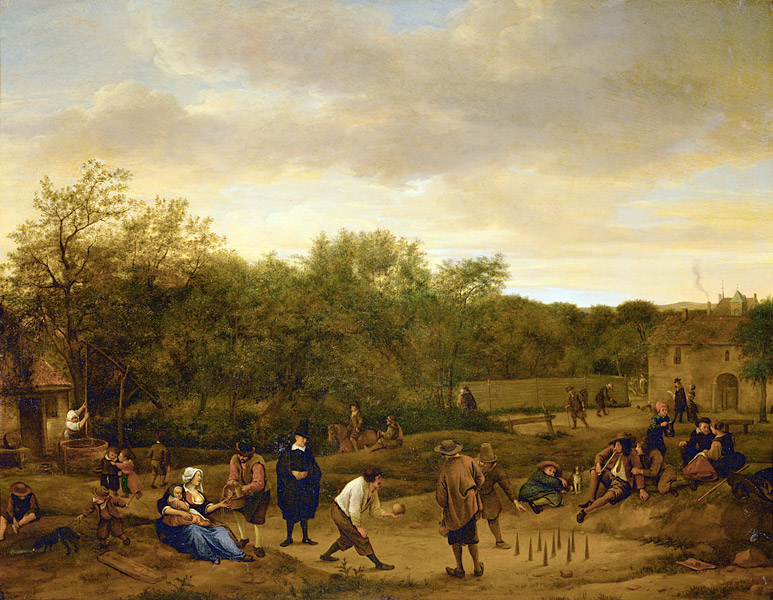
\includegraphics[width=6cm]{French.jpg}
      % \caption{}
    \end{figure}
    \pause
  \end{columns}

\end{frame}

\begin{frame}{概率论的诞生}
\begin{itemize}[<+-|alert@+>]
	\item Cardano虽说是概率的创派始祖, 但概率论真正变成一门学科的标志性事件则是1654年Pascal(帕斯卡)和Fermat(费马)关于两个赌博问题的通信.
	\item Pascal(帕斯卡)就是法国物理学家和数学家帕斯卡, 命名压强单位的物理学家Pascal.
	\item Fermat(费马)就是提出“费马大定理”并且困扰数学家300年之久的费马.
\end{itemize}



\end{frame}




\begin{frame}
  \frametitle{ 两个赌博问题}
  \begin{columns}
    \column{7.5cm}
    \begin{prob}De Mere(德梅尔):事件可能性大小
      \begin{itemize}[<+-|alert@+>]
      \item 一颗骰子投 4 次至少得到一个六点,
      \item 两颗骰子投 24 次至少得到一个双六.
      \end{itemize}
    \end{prob}
    \pause
    \begin{prob}  {\rm De Mere} 分赌注问题
      \begin{itemize}[<+-|alert@+>]
      \item 甲乙两人各下赌注$m$元;
      \item 甲乙两人获胜的概率一样,均为$\frac{1}{2}$;
      \item 先胜$t$局者取得全部赌金;
      \item 甲胜$a$局而乙胜$b$局时赌博被迫中止;
      \item 问赌注如何分?
      \end{itemize}
    \end{prob}
    \column{4cm}
    \vspace{-0.5cm}
    \begin{figure}[htbp]\nonumber


      \centering
      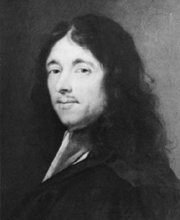
\includegraphics[width=3.5cm]{DeMere.jpg}
      \vspace{0cm}

      \centering{\rm Chevalier De Mere }


      % \caption{}
    \end{figure}
  \end{columns}
\end{frame}
\begin{frame}{骰子点数问题}
\begin{itemize}[<+-|alert@+>]
	\item 据经验所知,一颗骰子投 4 次至少得到一个六点的概率大于$\dfrac{1}{2}$;
	\item 两颗骰子掷一次的结果6倍于一颗骰子掷一次的结果, 则两颗骰子投 24 次至少得到一个双六的概率也应大于$\dfrac{1}{2}$;
	\item 但赌场经验却并非如此.%两颗骰子投 24 次至少得到一个双六的概率小于$\dfrac{1}{2}$;
	\item 考虑成功概率为$p$的随机试验, 连续做$n$次,我们来确定至少一次成功的概率为$q_0$对应的$n$:
	\[1-(1-p)^n=q_0\Rightarrow n=\dfrac{\ln(1-q_0)}{\ln(1-p)}=\dfrac{-\ln(1-q_0)}{p+\frac{p^2}{2}+\cdots}\approx \dfrac{-\ln(1-q_0)}{p};\]
	\item 两个不同成功概率的随机试验, 连续做$n$次, 要保其至少成功一次的概率相同所需要的$n$近似反比于单次试验成功的概率.
\end{itemize}


\end{frame}




\begin{frame}{分赌注问题历史}
	\vspace{-0.15cm}
\begin{itemize}[<+-|alert@+>]
	\item 分赌注问题最早是由意大利数学家Paccioli(帕乔利)在1494年提出, 当时Paccioli给出的答案是按$a:b$进行分配.
	\item 50年后, Tartaglia(塔尔塔利亚)提出反对意见:根据这条规则,如果游戏在一轮之后停止,那么其中一名玩家就会得到全部赌注.
	\item Tartaglia试图修改帕乔利的规则, 以便将上述情况考虑进去, 但最后他怀疑这个问题可能根本没有确定的答案.
	\item 1537年, Cardano也曾经思考过这个问题.
	\begin{itemize}[<+-|alert@+>]
		\item Cardano给出了一个公式$f(n)=1+...+n$, 甲还剩$s-a$局就可以获胜,乙还剩$s-b$局可以获胜, 两者的分金比率应该为$f(s-b):f(s-a)=(s-b)(s-b+1):(s-a)(s-a+1)$.
		%\item 若$s=6,a=5,b=3$, 则上述比为$6:1$.
		\item 虽然Cardano答案错误, 但Cardano已经开始考虑用未来剩余的赌局来决策,而不是局限于已发生的事件.
	\end{itemize}
    \item 直到1654年, De Mere向Pascal请教, Pascal和Fermat进行书信交流, 并且用不同的解法给出了这个问题的正确答案.
    \item 后来, 荷兰数学家Huygens也参与了Pascal和Fermat的讨论, 并在1657年出版书籍《De ratiociniis in ludo aleae ("On Reasoning in Games of Chance")》.

\end{itemize}


\end{frame}


\begin{frame}
  \frametitle{{\rm Blaise Pascal} (布莱士·帕斯卡)}
  \begin{columns}
    \column{4cm}
    % \vspace{2.5cm}
    \begin{figure}[htbp]\nonumber

      \centering
      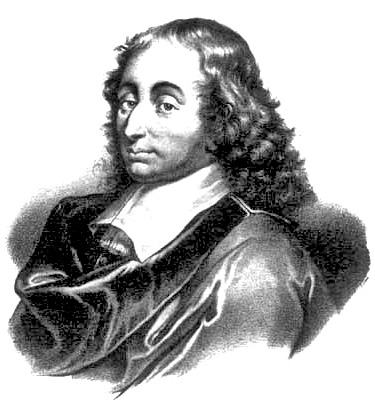
\includegraphics[width=4cm]{pascal1.jpg}

    \end{figure}
    \column{6.5cm}
    \begin{itemize}[<+-|alert@+>]
    \item 16 岁时发现著名的帕斯卡六边形定理:内接于一个二次曲线的六边形的三双对边的交点共线;
    \item 17 岁时写成《圆锥曲线论》,是研究德札尔格射影几何工作心得的论文;
    \item 设计并制作了一台能自动进位的加减法计算装置,被称为是世界上第一台数字计算器;
    \item 以积分学的原理解决了摆线问题;
    \item 与费马相互通信探求赌注分配问题,形成概率论中一个重要的基本概念—数学期望.
    \end{itemize}
  \end{columns}
\end{frame}



\begin{frame}
  \frametitle{{\rm Pierre de Fermat} (皮耶·德·费玛)}
  \begin{columns}
    \column{4cm}
    % \vspace{2.5cm}
    \begin{figure}[htbp]\nonumber

      \centering
      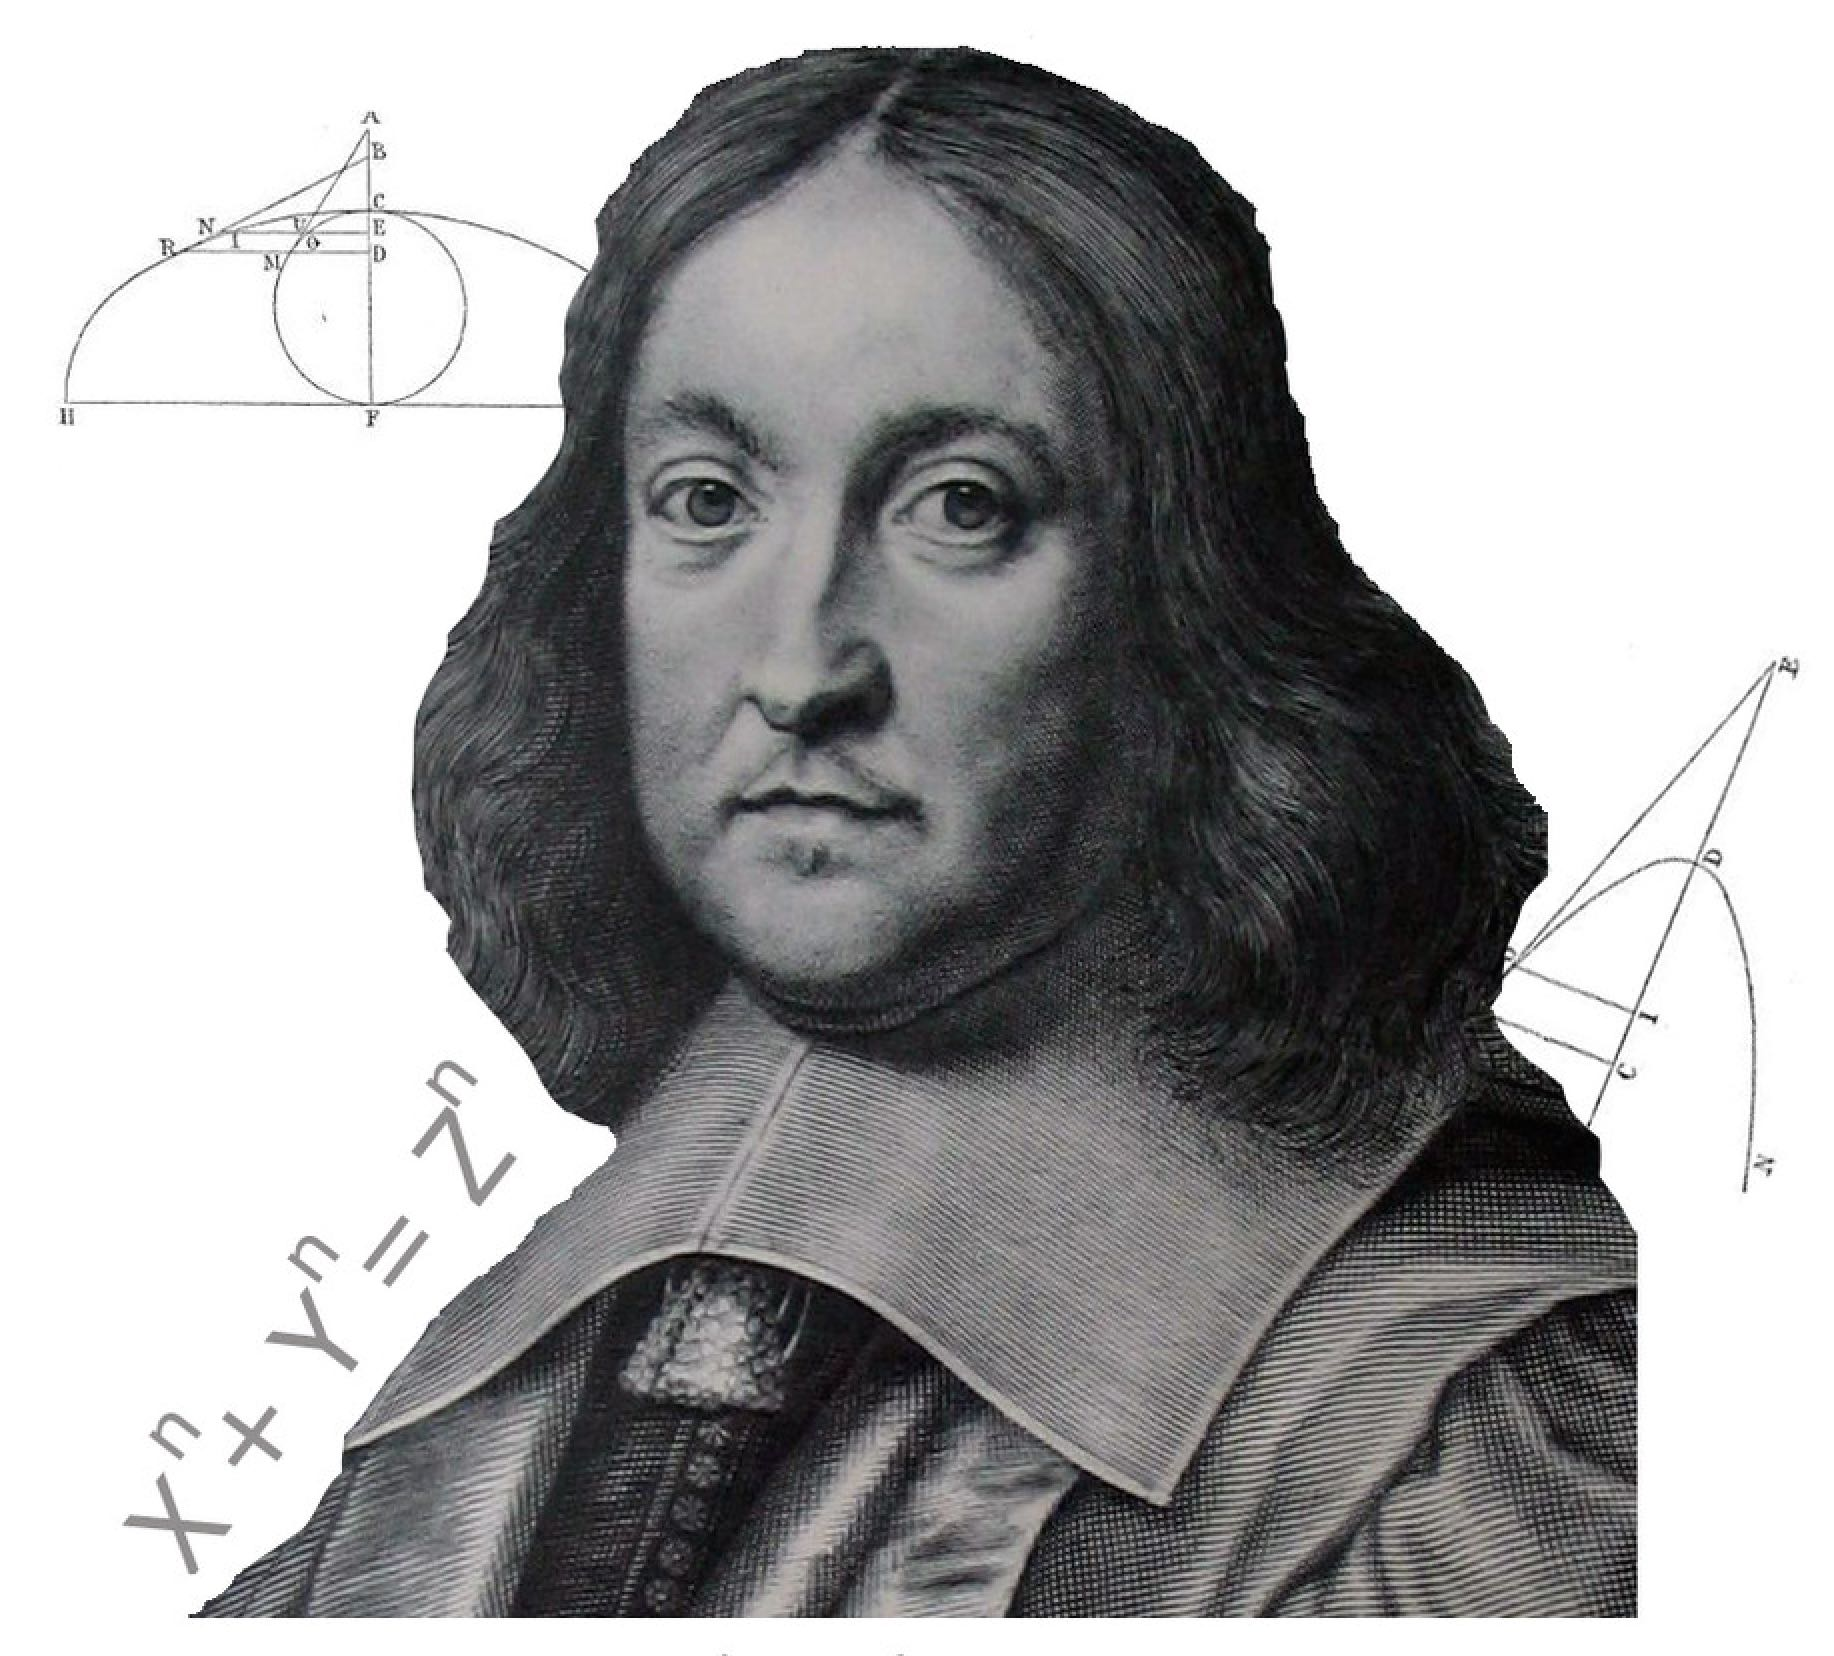
\includegraphics[width=4cm]{Fermat.jpg}

    \end{figure}
    \column{6.5cm}
    \begin{itemize}[<+-|alert@+>]
    \item 独立于笛卡儿发现了解析几何的基本原理;
    \item 求切线、求极大值和极小值以及定积分方法;
    \item 费马和帕斯卡在相互通信探求赌注分配问题,形成概率论中一个重要的基本概念—数学期望;
    \item 数论中的费马大小定理;
    \item 光学的最小作用原理.
    \end{itemize}
  \end{columns}
\end{frame}


\begin{frame}
  \frametitle{{\rm Christiaan Huygens }(克里斯蒂安·惠更斯)}
  \begin{columns}
    \column{6cm}
    \begin{itemize}[<+-|alert@+>]
    \item {\rm Christiaan Huygens} 在 1657 年写了世界上第一本关于概率论的著作 {\rm De ratiociniis in ludo aleae (``On Reasoning in Games of Chance")}, 中文译名``论赌博中的计算”.
    \item 概率论的基本概念、第一次在书中提出期望.
    \end{itemize}

    \column{4cm}
    \begin{figure}[htbp]
      \centering
      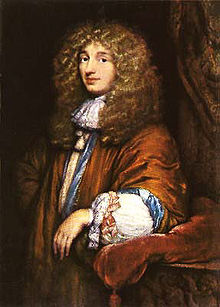
\includegraphics[width=3.5cm]{ChristiaanHuygens.jpg}
    \end{figure}
  \end{columns}
\end{frame}

\begin{frame}{分赌注问题:{\rm Fermat}解法}
\begin{itemize}[<+-|alert@+>]
	\item 显然甲乙距离赢得赌局分别还差$r=t-a$局和$s:=t-b$局. 因此,若赌局不终止,赌局肯定会在接下来的$r+s-1$轮内结束.
	\item 考虑所有$r+s-1$场赌局的结果, 计算在所有可能结果中,甲乙最终获胜的概率. 这样一来,整个问题就简化为一个古典概型的概率计算问题.%关于等概率情况的问题,通过计数就可以算出概率
	\item 以上述计算出来的获胜概率作为分配赌注的比例.
	\item 若$t=6,a=5,b=3$, 则最多还需要赌$3$场就可以分出胜负. 后续所有可能的结果分别为
	$$\{\text{甲甲甲,甲甲乙,甲乙甲,甲乙乙,乙甲甲,乙甲乙, 乙乙甲, 乙乙乙}\}.$$
	\item 所有的$7$种结果中, 乙只有一个结果获胜, 也就是连胜三局, 故赌注分配比例应为$7:1$.
\end{itemize}


\end{frame}

\begin{frame}{分赌注问题:{\rm Pascal}解法}
\begin{itemize}[<+-|alert@+>]
	\item 杨辉三角或Pascal三角法
	\begin{itemize}[<+-|alert@+>]
		\item 后续$r+s-1$场赌局的所有可能结果中:

		使得甲获胜的结果个数为: $n_{\text{甲}}=\sum_{k=r}^{r+s-1}C_{r+s-1}^k$

		使得乙获胜的结果个数为: $n_{\text{乙}}=\sum_{k=s}^{r+s-1}C_{r+s-1}^k$
		\item 若$t=6,a=5,b=3$即$r=1,s=3$, 则
		$$n_{\text{甲}}=C_3^1+C_3^2+C_3^3=7, \quad n_{\text{乙}}=C_3^3=1$$
	\end{itemize}


\end{itemize}

\end{frame}


\begin{frame}{分赌注问题:{\rm Pascal}解法}
	\begin{itemize}[<+-|alert@+>]
		\item 递推法
		\begin{itemize}[<+-|alert@+>]
			\item 假设甲和乙赌注共$64$个金币, 考虑$t=6,a=5,b=4$的情况:

			如果下一局甲胜,则甲得到全部64枚金币

			如果下一局甲输,则比分变为$5:5$, 这时候是平局,甲乙平分赌注.

			\item 不管哪种情况, 甲至少会拿$32$个金币,剩余的$32$个金币,可能归甲也可能归乙,平分. 这样甲应该拿$32+(64-32)/2=48$个金币,乙则拿$16$个金币.
			\item 考虑$t=6,a=5,b=3$的情况:
			\begin{itemize}[<+-|alert@+>]
				\item 如果下一局甲胜,则拿到所有赌注;
				\item 如果甲败,则问题转化为$t=6,a=5,b=4$的情况;
				\item 由此可见,甲至少可拿48个硬币,剩余金币平分;
				\item 因此,甲最终可拿$48+(64-48)/2=56$个金币, 乙拿8个金币;
				\item 和Fermat的$7:1$结果相同.
			\end{itemize}


			%\item Pascal分析了一个简化版本, 就是$t=3,a=2,b=1$的情况.
			%\item 假设甲和乙的赌注一共为$64$个金币, 当$2:1$比分的情况下:

			%%如果甲输了,则比分变成$2:2$,这时候是平局,甲乙平分奖金.

			%\item 不管哪一种情况, 甲至少会拿$32$个金币,至于剩余的$32$个金币,可能归甲也可能归乙,平分. 这样甲应该拿$32+(64-32)/2=48$个金币,乙则拿$16$个金币.

			%\item 考虑$t=6,a=5,b=4$的情况: 与$t=3,a=2,b=1$的情况类似, 甲应该拿$32+(64-32)/2=48$个金币.
		\item 在递推解法里,Pascal用到了期望的思想,尤其是$48+(64-48)/2$这个式子.
		\begin{itemize}[<+-|alert@+>]
			\item 下一局甲胜得到$x=64$个金币,甲输得到$y=48$个金币;
			\item 按Pascal的式子, 甲拿到的金币为: $y+(x-y)/2=(x+y)/2=x*0.5+y*0.5$,这其实就是条件期望公式.
		\end{itemize}

		\end{itemize}

	\end{itemize}

	\end{frame}

\begin{frame}{分赌注问题:{\rm Pascal}递推法的一般解法}
\begin{itemize}[<+-|alert@+>]
	\item 赌博中断时,甲乙距离赢得赌局分别还差$r=t-a$局和$s:=t-b$局;
	\item 假设中断后赌局继续进行, 甲最终获胜的概率记为$e(r,s)$, 则有边界条件:
	\[e(0,s)=1,\quad e(r,0)=0,\quad e(r,r)=1/2\]且有如下递推式
	\[e(r,s)=[e(r-1,s)+e(r,s-1)]/2.\]
	\item 上式用到了全概率公式,是一个偏差分方程. Pascal借助算术三角阵, 利用数学归纳法得到
	\[
	e(r, s)=\frac{D_{r+s-1, s-1}}{D_{r+s-1}} (r+s=2,3, \cdots)
	\]
	\item 这里分子表示算术三角形中第${r+s-1}$行最后${s}$项之和,而分母为第${r+s-1}$行的所有数字之和, 故为${2^{r+s-1}}$.
\end{itemize}


\end{frame}





\begin{frame}
  \frametitle{{\rm Jacob Bernoulli}(雅各布·伯努利)}
  \begin{columns}
    \column{6cm}
    \begin{itemize}[<+-|alert@+>]
    \item 概率论与变分法先驱之一;
    \item 第一次使用``积分"一词;
    \item 首次给出直角坐标和极坐标下的曲率半径公式;
    \item 1713 年出版 《Ars Conjectandi》(可译为《猜度术》):提出了概率论中的“伯努利大数定律” - 大数定律的最早形式.
    \end{itemize}

    \column{5cm}

    \begin{figure}[htbp]
      \centering
      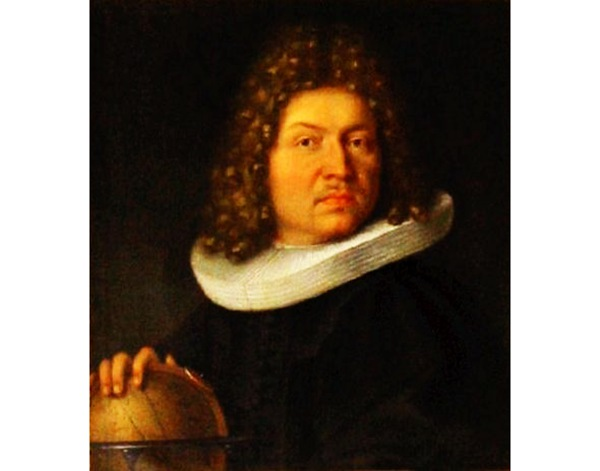
\includegraphics[width=5.5cm]{Bernoulli.jpg}
    \end{figure}
  \end{columns}
\end{frame}



\begin{frame}
  \frametitle{{\rm Abraham de Moivre}(亚伯拉罕·棣莫弗)}
  \vspace{-0.15cm}
  \begin{columns}
    \column{6.5cm}
    \begin{itemize}[<+-|alert@+>]
    \item 棣莫弗公式:$$(\cos x+i\sin x)^n=\cos(nx)+i \sin(nx)$$

    \item 二项分布的正态逼近:棣莫弗-拉普拉斯中心极限定理;
    \item 利用概率生成函数计算均匀分布随机变量和的分布;
    \item 寿险保险数学:年金的分析与计算.
    \item 开创了概率论的现代方法:1718 年发表了《The Doctrine of Chance》. 在此书中
	统计独立性的定义首次出现. 该书在 1738 年与 1756 年出了扩展版,生日问
	题出现在 1738 年的版本中,赌徒破产问题出现在 1756 年的版本中.
    \end{itemize}

    \column{5cm}

    \begin{figure}[htbp]
      \centering
      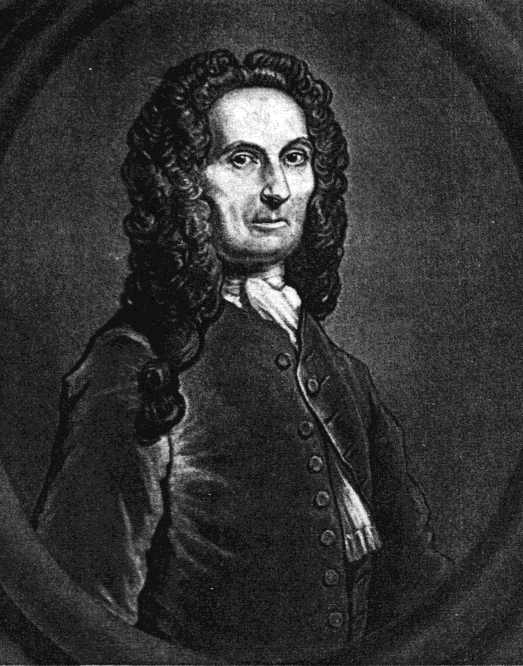
\includegraphics[width=4.5cm]{deMoivre.jpg}
    \end{figure}
  \end{columns}
\end{frame}












\begin{frame}
  \frametitle{{\rm Pierre-Simon Laplace}(皮埃尔-西蒙·拉普拉斯)}
  \begin{columns}
    \column{6cm}
    \begin{itemize}[<+-|alert@+>]
    \item {\rm Pierre-Simon Laplace} 在他 1812 年的著作{\rm 《Th{\'e}orie Analytique des Probabilit{\`i}{\'e}s》}(可
	译为《概率论的解析理论》)中介绍了概率的数学理论及其科学应用;

    \item {\rm Laplace}只考虑了古典概型, 对一般的概率及其应用没有介绍;
    \item 到 1850 年, 许多数学家发现古典概型对一般场合不合理, 开始尝试重新定义概率.
    \end{itemize}

    \column{5cm}

    \begin{figure}[htbp]
      \centering
      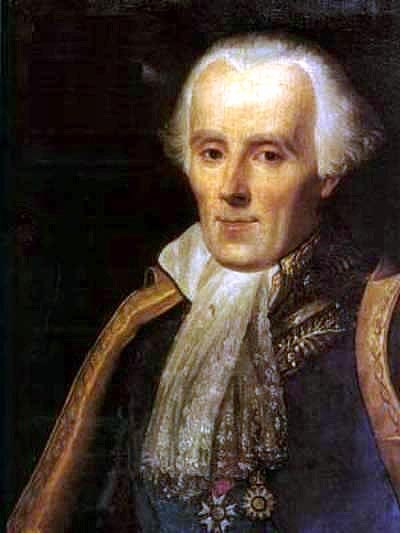
\includegraphics[width=4.5cm]{Laplace.jpg}
    \end{figure}
  \end{columns}
\end{frame}




\begin{frame}{概率的公理化体系}

\begin{itemize}[<+-|alert@+>]
    \item  从 17 世纪到 19 世纪长达 300 多年的时间里,以 Laplace(1749 一
1827), De Moivre(1687-1754), J.Bernouil, D.Bernouli(1700--1782).
Pascal、Fermat 等为代表的优秀学者从各自不同的角度对概率论的许多方面进行了深入细致的研究,取得了大量成果,可是都无法将概率论纳入到严格的公理化体系中.而概率论作为数学的重要分支,其逻辑的严密性和完整性始终受到质疑.
\item 数学大师 Hilbert(1862—1943)在 1900 年提出的 23 个著名问题中,第 6 个问题是关于“物理定律的公理化”,其中就涉及概率论的公理化问题.
\item 激发了以 Borel(1871 一 1956)和 Lebesgue(1875—1941)等为代表的一批学者的研究热情.他们在测度理论(Measure Theory)方面得到的成果为后续研究指明了道路.
\end{itemize}
\end{frame}





\begin{frame}
  \frametitle{{\rm Andrey Kolmogorov}(安德列·柯尔莫哥洛夫)}
  \begin{columns}
    \column{6cm}
    \begin{itemize}[<+-|alert@+>]
    \item {\rm Andrey Kolmogorov} 第一个在他 1933 年的著作{\rm 《Grundbegriffe der Wahrscheinlichkeitsrechnun》(《Foundations of the Theory of Probability》)} 中严格的定义了概率;
    \item 类似于{\rm Euclid}基于公理体系建立几何, 他从基本公理建立了概率理论, 从而使概率论称为一门严谨的数学分支;
    \item 概率理论的现代研究和测度论非常紧密的结合在一起.

    \end{itemize}

    \column{5cm}

    \begin{figure}[htbp]\nonumber
      \centering
      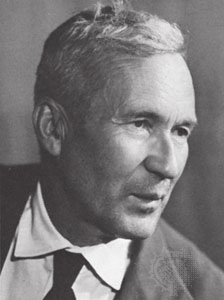
\includegraphics[width=4cm]{Kolmogorov.jpg}

      \centering{\rm 1903.4.25-1987.10.20}

    \end{figure}
  \end{columns}
\end{frame}
\begin{frame}
  \frametitle{{\rm Kolmogorov} 成就}
  \vspace{-0.4cm}
  {\small\begin{itemize}[<+-|alert@+>]
    \item 20 世纪最伟大的数学家之一,在概率论、实分析、拓扑学、泛函分析、微分方程、生物数学、等很多领域都有着开创性的贡献.

    \item 1933 年,出版《概率论基础》,首次将概率论建立在严格的公理基础上,解决了希尔伯特第 6 问题的概率部分。
    \item 线性拓扑空间理论的创始人之一, 和美国著名数学家亚历山大({\rm J.W.Alexander})同时独立引入上同调群的概念;

    \item 40 年代, 在遗传学、弹道学、气象学、金属结晶学等有重要贡献;
    \item 50 年代, 经典力学、遍历理论、函数论、信息论、算法理论等。

    \item 柯尔莫哥洛夫的研究几乎遍及数论之外的一切数学领域。1963 年,在第比利斯召开的概率统计会议上,美国统计学家沃尔夫维茨({\rm J.Wolfowitz})说:``我来苏联的一个特别的目的是确定柯尔莫哥洛夫到底是一个人呢,还是一个研究机构.”


    \end{itemize}}
\end{frame}

\begin{frame}
  \frametitle{{\rm Kolmogorov} 轶事}
  \begin{itemize}[<+-|alert@+>]
  \item  历史学要证实自己的观点需要几个甚至几十个正确证明才行,数学只需要一个证明就行, 于是转行数学.
  \item 20 年代的莫斯科大学,学生被要求在十四个不同的数学分支参加十四门考试;但考试可用相应领域的独立研究代替. {\rm Kolmogorov} 从来没有参加考试,他写了十四个不同方向的有新意的文章。
  \item {\rm Kolmogorov}总是以感激的口气提到斯大林:“首先,他在战争年代为每一位院士提供了一床毛毯;第二,原谅了我在科学院的那次打架。”{\rm Kolmogorov}一次在选举会上打了{\rm Luzin}(卢津)一个耳光,他说:“(打架)那是我们常用的方式。”{\rm Luzin}在实变函数方面有着很重要的贡献,但是以打架而论,远非{\rm Kolmogorov}的对手.
  \end{itemize}
\end{frame}



 

\title[概率论]{第二讲:事件及其运算关系}
%\author[张鑫{\rm Email: xzhangseu@seu.edu.cn} ]{\large 张 鑫}
%\institute[东南大学数学学院]{\large 张鑫\\ \quad \\ \textrm{Email: xzhangseu@seu.edu.cn} \\ \quad  \\
\institute[东南大学数学学院]{\large \textrm{Email: xzhangseu@seu.edu.cn} \\ \quad  \\
  \large 东南大学\quad 数学学院\\
  \vspace{0.3cm}
 % \trc{ 公共邮箱: \textrm{zy.prob@qq.com}\\
  %  \hspace{-1.7cm}  密\qquad 码: \textrm{seu!prob}}
}
%\date{\rm \today}
\date{}


{ \setbeamertemplate{footline}{}
  \begin{frame}
    \titlepage
  \end{frame}
}

\section{事件与概率}







\subsection{样本空间与随机事件}
\begin{frame}
  \frametitle{概率: (随机)事件发生的可能性大小的度量}
  \begin{itemize}[<+-|alert@+>]
  \item \textcolor{cyan}{随机现象:} 一定条件下,并不总是出现相同结果的现象, 比如抛一枚硬币,掷一颗骰子等;
  \item \textcolor{cyan}{随机试验:} 随机现象的实现和对它某个特征的观测; 常简称\textcolor{cyan}{试验}    \begin{itemize}[<+-|alert@+>]
    \item 随机试验中要求试验的结果至少 2 个;

    \item 每次试验或观测得到其中的一个结果,在试验或观测之前不能预知是哪个结果发生;

    \item 一般还要求试验在相同条件下能够重复.
    \item 比如:观测把硬币抛 4 次后正面向上的次数; 观测某地的温度变化; 某电话总机单位时间内转接的电话次数.
    \end{itemize}
  \end{itemize}
\end{frame}

\begin{frame}
	\frametitle{样本点与样本空间}
	\begin{itemize}[<+-|alert@+>]
		\item \textcolor{cyan}{样本点({\rm Sample Point}):} 随机试验的每个可能结果称为一个样本点,常用\textcolor{red}{$\omega$}表示.
		\item \textcolor{cyan}{样本空间({\rm Sample Space}):} 全体样本点构成的集合, 常用\textcolor{red}{$\Omega$}表示.
	\begin{itemize}[<+-|alert@+>]
		\item 一个试验的样本空间可能是有限的,可数无限的或不可数的;
		\item 当样本空间为有限的时, 我们可以将样本点可视化为圆点,做一次试验就等同于随机选取一个圆点;
		\item 如果所有的圆点都是相同的,那么所有的圆点被抽中的可能性就相同,即后面将要介绍的古典概型.
	\end{itemize}
	\end{itemize}
\end{frame}




\begin{frame}
  \frametitle{事件}
  \begin{itemize}[<+-|alert@+>]

  \item \textcolor{cyan}{随机事件:} 简称事件 ({\rm Event}), 由部分样本点组成的试验结果
  \begin{itemize}[<+-|alert@+>]
  	\item 通常指在随机试验中我们所关心的某一部分可能结果
  	\item  如果按照样本点可视化为圆点,则事件就是一些圆点的集合
	\end{itemize}
  \item \textcolor{cyan}{基本事件:} 仅含有一个样本点的随机事件称为基本事件, 它犹如分子中的原子, 在化学反应中不能再分, 所以有 ``基本'' 两字.
  \item \textcolor{cyan}{事件发生}
    \begin{itemize}[<+-|alert@+>]
    \item \textcolor{cyan}{事件$A$发生}:事件$A$包含的样本点在随机试验结果中出现即$\omega\in A$;
    \item 通常把事件$A$所包含的样本点构成的集合与事件$A$视为等同,也记为$A$,
    \end{itemize}
  \item \textcolor{cyan}{两个特殊的事件:}
    \begin{itemize}[<+-|alert@+>]
    \item \textcolor{cyan}{必然事件}($\Omega$):在随机试验中一定会发生的事件;
    \item \textcolor{cyan}{不可能事件}($\emptyset$):在随机试验中不可能发生的事件;
    \end{itemize}
  \end{itemize}
\end{frame}
\begin{frame}
  \frametitle{硬币抛 3 次的随机试验}
  \begin{itemize}[<+-|alert@+>]
  \item \textcolor{cyan}{样本点:}正正正、正正反、正反正、反正正、正反反、反正反、反反正、反反反,共 8 种可能结果;
  \item \textcolor{cyan}{基本事件:} \{正正正\}、\{正正反\}、\{正反正\}、 \{反正正\}、\{正反反\}、\{反正反\}、\{反反正\}、\{反反反\}, 共 8 个基本事件;
  \item \tc{ 样本空间 $\Omega$:}
   {\small\[\Omega:=\{\mbox{正正正,正正反,正反正,反正正,正反反,反正反,反反正,反反反}\}\]}
  \item \textcolor{cyan}{随机事件:}
    \begin{eqnarray*}
      A&:=&\{\mbox{至少出现两次正面}\}\\
       &=&\{\mbox{正正正,正正反,正反正,反正正}\} \\
      B&:=&\{\mbox{三次均为正面}\}=\{\mbox{正正正}\}\\
      \cdots
    \end{eqnarray*}
  \end{itemize}
\end{frame}


\begin{frame}
  \frametitle{样本空间示例}
  \begin{itemize}[<+-|alert@+>]
  \item 掷一枚骰子, 观察出现的点数. 则 $\Omega=\{1, 2, 3, 4, 5, 6\}$.
  \item 考察某一地区的年降雨量,则$\Omega=\{x|0\le x<T\}$,这里$T$表示某个常数, 表示降雨量不会超过$T$.
  \item 将一枚硬币抛两次,考察正反面出现的情况, 则 \[\Omega=\{\mbox{正正,正反,反正,反反}\}.\]
  \item 将一枚硬币抛两次,考察正面出现的次数, 则$\Omega=\{0, 1, 2\}$.
  \item 先后掷两次骰子,考察两次骰子的点数, 则
  $$\Omega=\{(a_1, a_2), a_i\in \{1,2,\cdots, 6\}, i=1,2\}.$$
  \end{itemize}
\end{frame}
\subsection{事件的运算与关系}
\begin{frame}
  \frametitle{事件间的并:$A\cup B$}
  % \begin{columns}
  %   \column{5cm}

  \begin{defi} (\tc{ 事件$A$与事件$B$的并}) 记为 $A\cup B$, 其含义为:事件$A$和事件$B$至少有一个发生, 即由事件$A$与$B$中所有的样本点组成的新事件.\pause 用数学符号来描述即为:
    \begin{eqnarray*}
      A\cup B:=\{\omega\in \Omega: \omega\in A, \mbox{ 或 } \omega\in B\}
    \end{eqnarray*}
  \end{defi}
  \vspace{-0.7cm}
  \only<2->{\begin{figure}[htbp]\nonumber

    \centering
    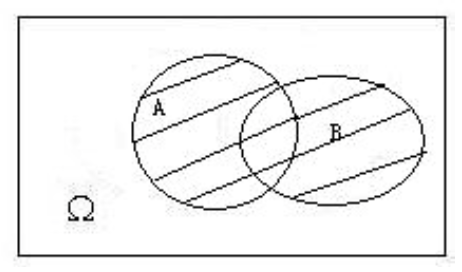
\includegraphics[width=3cm]{bing.png}

  \end{figure}}

  % \column{4cm}
  \pause
  \begin{exam}
    考虑掷一枚骰子, 观察出现的点数. 记事件$A$为掷出的点数为奇数, 事件$B$为掷出的点数不超过$3$, 则
    \[A=\{1,3,5\},\quad  B=\{1,2,3\},\quad  A\cup B=\{1,2,3,5\}\]

  \end{exam}


  % \end{columns}
\end{frame}
%\subsection{事件及其运算关系}

\begin{frame}
  \frametitle{事件间的交:$A\cap B$}
  % \begin{columns}
  %   \column{5cm}

  \begin{defi} (\tc{ 事件$A$与事件$B$的交}) 记为 $A\cap B$或 $AB$, 其含义为:事件$A$和事件$B$同时发生, 即由事件$A$与$B$中公共的样本点组成的新事件.\pause 用数学符号来描述即为:
    \begin{eqnarray*}
      A\cap B:=\{\omega\in \Omega: \omega\in A \mbox{ 且 } \omega\in B\}
    \end{eqnarray*}
  \end{defi}
  \vspace{-0.7cm}
  \only<2->{\begin{figure}[htbp]\nonumber
    \centering
    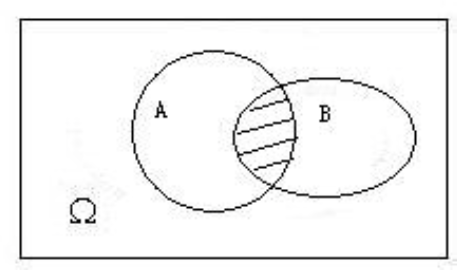
\includegraphics[width=3cm]{jiao.png}
  \end{figure}}

  % \column{4cm}
  \pause
  \begin{exam}
    考虑掷一枚骰子, 观察出现的点数. 记事件$A$为掷出的点数为奇数, 事件$B$为掷出的点数不超过$3$, 则
    \[A=\{1,3,5\},\quad  B=\{1,2,3\},\quad  A\cap B=\{1,3\}\]

  \end{exam}

\end{frame}


\begin{frame}
  \frametitle{事件的差:$A-B$}
  % \begin{columns}
  %   \column{5cm}

  \begin{defi} (\tc{ 事件$A$与$B$的差}) 记为$A-B$或$A\backslash B$, 其含义为:事件$A$发生且事件$B$不发生, 即由在$A$中而不在$B$中的样本点组成的新事件. \pause 用数学符号来描述即为:
    \begin{eqnarray*}
      A-B:=\{\omega\in \Omega: \omega\in  A \mbox{ 且 } \omega\notin B\}
    \end{eqnarray*}
  \end{defi}
  \vspace{-0.7cm}
  \only<2->{\begin{figure}[htbp]\nonumber

    \centering
    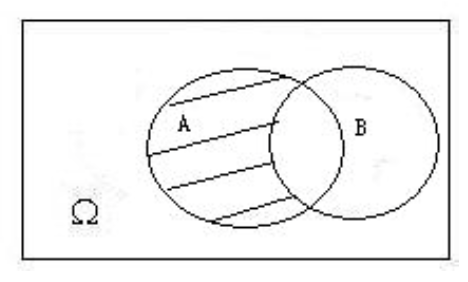
\includegraphics[width=3cm]{cha.png}

  \end{figure}}

  % \column{4cm}
  \pause
  \begin{exam}
    考虑掷一枚骰子, 观察出现的点数. 记事件$A$为掷出的点数为奇数, 事件$B$为掷出的点数不超过$3$, 则
    \[A=\{1,3,5\},\quad  B=\{1,2,3\},\quad  A-B=\{5\}\]   \end{exam}

\end{frame}


\begin{frame}
  \frametitle{对立事件:$\overline{A}$}
  % \begin{columns}
  %   \column{5cm}

  \begin{defi} (\tc{ 事件$A$的对立事件}) 记为$\overline{A}$或$A^c$, 其含义为:事件$A$不发生, 即由在$\Omega$中而不在$A$中的样本点组成的新事件.\pause 用数学符号来描述即为:
    \begin{eqnarray*}
      \overline{A}:=\{\omega\in \Omega: \omega\notin  A\}\textcolor{red}{=\Omega-A}
    \end{eqnarray*}
  \end{defi}
  \vspace{-0.7cm}
  \only<2->{ \begin{figure}[htbp]\nonumber

    \centering
    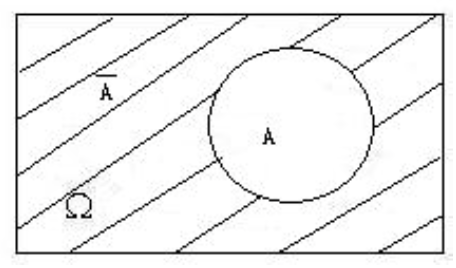
\includegraphics[width=3cm]{bu.png}

  \end{figure}}

  % \column{4cm}
  \pause
  \begin{exam}
    考虑掷一枚骰子, 观察出现的点数. 记事件$A$为掷出的点数为奇数, 则
    \[A=\{1,3,5\},\quad \overline{A}=\{2,4,6\}\]

  \end{exam}

\end{frame}
\begin{frame}
	\frametitle{对称差事件:$A\Delta B$}
	% \begin{columns}
		%   \column{5cm}

		\begin{defi} (\tc{ 事件$A$与$B$的对称差事件}) 记为$A\Delta B$, 其含义为:事件$A$与$B$中恰有一个事件发生.\pause 用数学符号来描述即为:
			\begin{eqnarray*}
				A\Delta B:=\{\omega\in \Omega: \omega\in A\cup B \mbox{ 且 } \omega\notin A\cap B\}\textcolor{red}{=(A-B)\cup (B-A)}
			\end{eqnarray*}
		\end{defi}
%		\vspace{-0.7cm}
%		\only<2->{ \begin{figure}[htbp]\nonumber
%
%				\centering
%				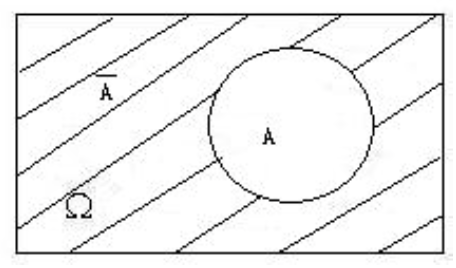
\includegraphics[width=3cm]{bu.png}
%
%		\end{figure}}
%
%		% \column{4cm}
%		\pause
%		\begin{exam}
%			考虑掷一枚骰子, 观察出现的点数. 记事件$A$为掷出的点数为奇数, 则
%			\[A=\{1,3,5\},\quad \overline{A}=\{2,4,6\}\]
%
%		\end{exam}

	\end{frame}


\begin{frame}
  \frametitle{包含关系: $A\subset B$}
  \begin{defi} (\tc{ 包含关系}) 称事件$A$包含于事件$B$,或事件$B$包含事件$A$(记为\tc{$A\subset B$}), 如果事件$A$发生必然导致事件$B$发生, 即属于$A$的样本点必然属于$B$.
  \end{defi}
  \pause
  \begin{exam}
    考虑掷一枚骰子, 观察出现的点数. 记事件$A$为掷出的点数为$2$或$4$, 事件$B$为掷出的点数为偶数. 则显然有事件$A$发生必然导致事件$B$发生,同时易知
    \begin{eqnarray*}
      A=\{2,4\}\subset \{2,4,6\}=B
    \end{eqnarray*}
  \end{exam}
\end{frame}

\begin{frame}
  \frametitle{相等关系: $A=B$}
  \begin{defi} (\tc{相等关系}) 称事件$A$与事件$B$相等(记为\tc{$A=B$}), 如果$A\subset B$且$B\subset A$, 即事情件$A,B$有相同的样本点.
  \end{defi}

  \pause
  \begin{exam}
    考虑掷一枚骰子, 观察出现的点数. 记事件$A$为掷出的点数为$2,4,6$, 事件$B$为掷出的点数为偶数. 则显然有
    \[A\subset B, B\subset A,\] 同时易有
    \begin{eqnarray*}
      A=\{2,4, 6\}=\{2,4,6\}=B
    \end{eqnarray*}

  \end{exam}
\end{frame}
\begin{frame}
  \frametitle{互不相容关系: $A\cap B=\emptyset$}
  \begin{defi} (\tc{ 互不相容关系}) 称事件$A$与事件$B$互不相容, 如果事件$A, B$不能同时发生, 即事情件$A,B$没有相同的样本点.
  \end{defi}

  \pause
  \vspace{1cm}
  \begin{exam}
    考虑掷一枚骰子, 观察出现的点数. 记事件$A$为掷出的点数为奇数, 事件$B$为掷出的点数为偶数. 则显然有事件$A,B$互不相容, 并且
    \begin{eqnarray*}
      A\cap B=\{1,3,5\}\cap \{2,4,6\}=\emptyset
    \end{eqnarray*}

  \end{exam}
\end{frame}

\begin{frame}
  \frametitle{对立事件与互不相容事件}
  \begin{itemize}[<+-|alert@+>]
  \item $\overline{\overline{A}}=A, A\cap \overline{A}=\emptyset, A\cup \overline{A}=\Omega$;
  \item $A,B$互为对立事件的充要条件为$A\cap B=\emptyset, A\cup B=\Omega$;
  \item 对立事件一定是互不相容事件, 但互不相容事件不一定是对立事件;
  \item $A-B=A\cap \overline{B}=A\overline{B}$
  \end{itemize}
\end{frame}

\begin{frame}{多个事件的运算}
	\begin{itemize}[<+-|alert@+>]

		\item 有限并事件:$\bigcup_{k=1}^{n}A_{k}$%:表示$n$个事件$A_1,A_2,...,A_n$至少有一个发生
		\item 有限交事件:$\bigcap_{k=1}^{n}A_{k}$%:表示$n$个事件$A_1,A_2,...,A_n$同时发生
		\item 可列并事件:$\bigcup_{k=1}^{\infty}A_{k}$%:$A_{1} \cup A_{2} \cup \cdots=\bigcup_{k=1}^{\infty} A_{k}=\lim _{n \rightarrow \infty} \bigcup_{k=1}^{n} A_{k}$
		\item 可列交事件:$\bigcap_{k=1}^{\infty}A_{k}$%:$A_{1} \cap A_{2} \cap \cdots=\bigcap_{k=1}^{\infty} A_{k}=\lim _{n \rightarrow \infty} \bigcap_{k=1}^{n} A_{k}$
		%\item 上极限事件$\bigcap_{k=1}^{\infty} \bigcup_{n=k}^{\infty} A_{n}$,其中$\left\{A_n,n\in\mathbb{Z}^+\right\}$是一列事件
		%\item 下极限事件$\bigcup_{k=1}^{\infty} \bigcap_{n=k}^{\infty} A_{n}$,其中$\left\{A_n,n\in\mathbb{Z}^+\right\}$是一列事件
	\end{itemize}
\end{frame}


\begin{frame}
	\frametitle{事件运算的性质}
	\begin{enumerate}[<+-|alert@+>][(1)]
		\item \tc{ 交换律:} $A\cup B=B\cup A, AB=BA$;
		\item \tc{ 结合律:} $A\cup (B\cup C)=(A\cup B)\cup C, (AB)C=A(BC)$;
		\item \tc{ 分配律:} $(A\cup B)\cap C=(A\cap C)\cup (B\cap C)$, \\\qquad \qquad $(A\cap B)\cup C=(A\cup C)\cap (B\cup C)$;
		\item \tc{{\rm De Morgan} 对偶法则:}
		\begin{eqnarray*}
			\overline{\bigcup_{i=1}^nA_i}=\bigcap_{i=1}^n \overline{A}_i\\
			\overline{\bigcap_{i=1}^nA_i}=\bigcup_{i=1}^n \overline{A}_i
		\end{eqnarray*}
	\end{enumerate}
\end{frame}


\subsection{事件列的上下极限及其性质}

\begin{frame}
	\frametitle{事件列的上下极限}
	\begin{defi}
		令$A_n\subset \Omega, n\geq 1$为一列集合(事件), 记
		\begin{eqnarray*}
			\inf_{k\geq n} A_k:=\cap_{k=n}^\infty A_k,\quad  \sup_{k\geq n}A_k:=\cup_{k=n}^\infty A_k
		\end{eqnarray*}
		则事件列$A_n$的上下极限定义如下:
		\begin{eqnarray*}
			\liminf_{n\rightarrow\infty}A_n:=\cup_{n=1}^\infty\cap_{k=n}^\infty A_k,\\%=\lim_{n\rightarrow\infty}\bigg(\inf_{k\geq n}A_k\bigg)\\
			\limsup_{n\rightarrow\infty}A_n:=\cap_{n=1}^\infty\cup_{k=n}^\infty A_k.
		\end{eqnarray*}
		若
		\begin{eqnarray*}
			\liminf_{n\rightarrow\infty}A_n=\limsup_{n\rightarrow\infty}A_n=A
		\end{eqnarray*}
		则称$A$为事件列$\{A_n,n\geq 1\}$的极限,并记作$\lim_{n\rightarrow\infty}A_n=A$.
	\end{defi}

\end{frame}


\begin{frame}
	\frametitle{单调事件列的极限}
	\begin{defi}
		事件列$\{A_n\}$称为单调不减的,如果对任意的$n$均有$A_n\subset A_{n+1}$;     事件列$\{A_n\}$称为单调不增的,如果对任意的$n$均有$A_{n+1}\subset A_n$;
	\end{defi}
	\vspace{0.4cm}

	\pause


	\begin{thm}
		假设$\{A_n\}$是单调事件列,则
		\begin{enumerate}
			\item 如果$\{A_n\}$是单调不减事件列,则$\lim_{n\rightarrow\infty}A_n=\cup_{n=1}^\infty A_n$
			\item 如果$\{A_n\}$是单调不增事件列,则$\lim_{n\rightarrow\infty}A_n=\cap_{n=1}^\infty A_n$
		\end{enumerate}

	\end{thm}

\end{frame}


\begin{frame}
	\frametitle{示性函数({\rm indicator function})}
	\begin{defi}
		设$A\subset \Omega$, 我们定义事件(集合)$A$的示性函数如下
		\begin{eqnarray*}
			1_A(\omega)=\left\{
			\begin{array}[l]{ll}
				1, &\mbox{如果}\omega\in A;\\
				0, &\mbox{如果}\omega\notin A.
			\end{array}
			\right.
		\end{eqnarray*}

	\end{defi}

	\begin{rmk}
		\begin{itemize}[<+-|alert@+>]

			\item $A=\{\omega: 1_A(\omega)=1\}$;
			\item $1_A\leq 1_B\Leftrightarrow A\subset B$;
			\item $1_{A\cap B}=1_A\cdot 1_B$;
			\item $1_{A\cup B}=1_A+1_B-1_{A\cap B}$;
		\end{itemize}
	\end{rmk}
\end{frame}

\begin{frame}
	\frametitle{事件列上下极限的性质}
	\begin{lem}
		令$\{A_n\}$为$\Omega$的任一子集列,则
		\begin{eqnarray*}
			\limsup_{n\rightarrow\infty}A_n&=&\{\omega:\sum_{n=1}^\infty 1_{A_n}(\omega)=\infty\}\\
			&=&\{\omega: \omega\mbox{属于无穷多个}A_n\}\\
			\liminf_{n\rightarrow\infty}A_n&=&\{\omega:\sum_{n=1}^\infty 1_{\bar{A_n}}(\omega)<\infty\}\\
			&=&\{\omega:\mbox{除去有限多个}A_n\mbox{外},\omega\mbox{属于余下所有的}A_n\}
		\end{eqnarray*}
	\end{lem}\pause
	\zheng 由$\omega\in \limsup_{n\rightarrow\infty}A_n=\cap_{n=1}^\infty \cup_{k=n}^\infty A_k$知,对任意的$n$, 存在 $k_n\geq n$使得$\omega\in A_{k_n}$, 从而$\sum_{n=1}^\infty 1_{A_n}\geq \sum_{n=1}^\infty 1_{A_{k_n}}=\infty $.\pause

	\qquad 反之,若 $\omega\in \{\omega:\sum_{n=1}^\infty 1_{A_n}(\omega)=\infty\}$, 则存在$k_n\rightarrow\infty$使得$\omega\in A_{k_n}$, 从而对任意的$n$, $\omega\in\cup_{k=n}^\infty A_k$, 即 $$\omega\in \cap_{n=1}^\infty \cup_{k=n}^\infty A_k=\limsup_{n\rightarrow\infty} A_n.$$
\end{frame}


\subsection{事件运算表及例子}

\begin{frame}
	\frametitle{事件运算表}
	% \begin{columns}
		%   \column{5cm}

	\begin{figure}[htbp]\nonumber

				\centering
				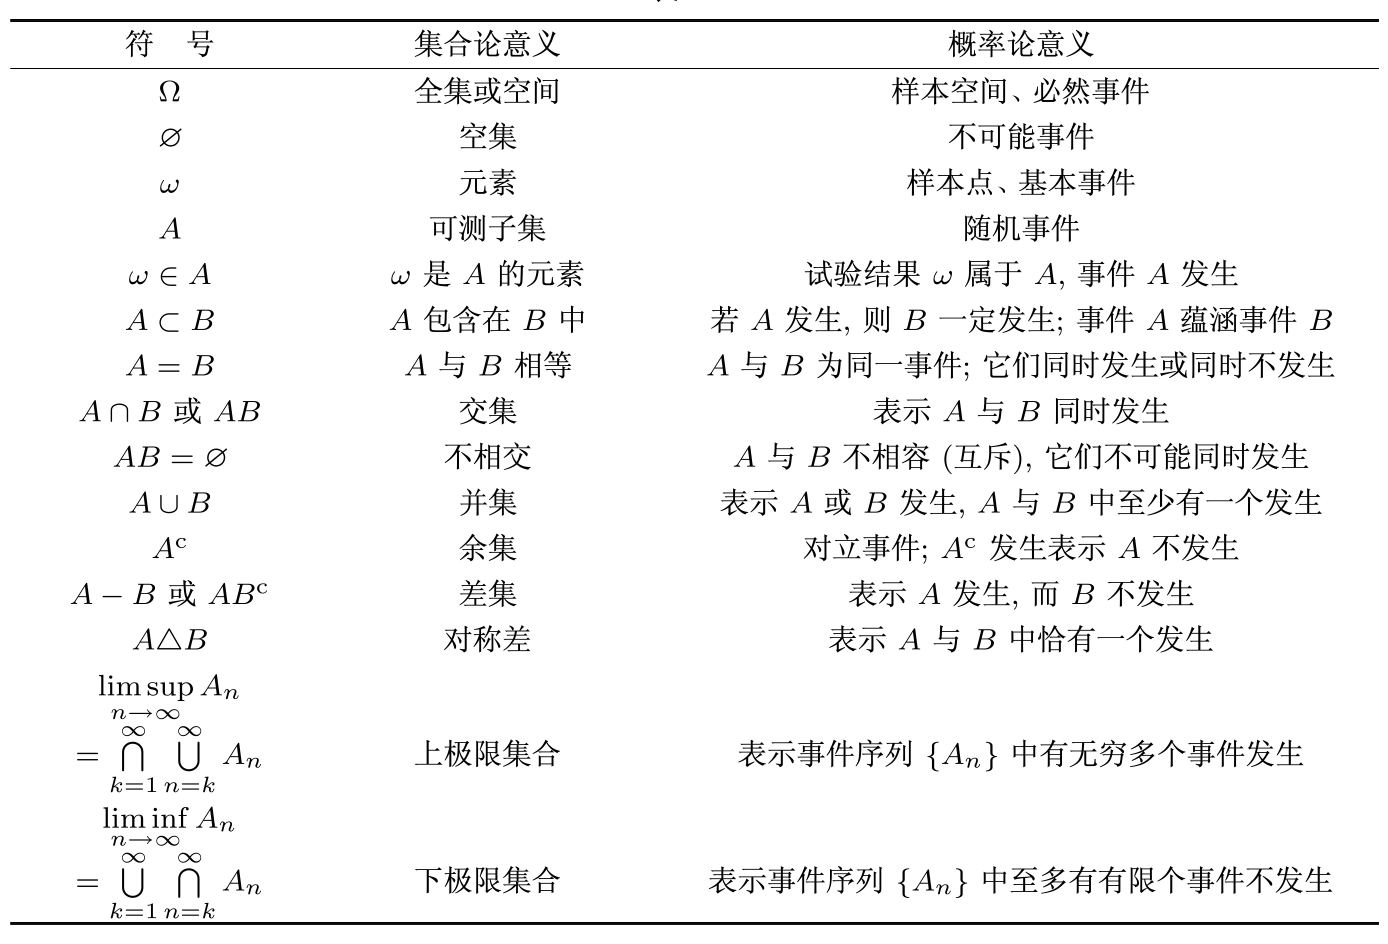
\includegraphics[width=12cm,height=7cm]{eventable.png}

		\end{figure}

	\vspace{1cm}
	\end{frame}










\begin{frame}
  \begin{exam}
    设$A,B,C$为某个随机现象的三个事件,试用事件的交,差,并,对立事件表示下列事件
    \begin{itemize}[<+-|alert@+>]
    \item 事件$A,B$发生而$C$不发生:\pause\textcolor{red}{$AB\overline{C}$};
    \item 事件$A,B,C$中至少有一个发生:\pause \trc{$A\cup B\cup C$};
    \item 事件$A,B,C$中至少有两个发生:\pause \trc{ $AB\cup AC\cup BC$};
    \item 事件$A,B, C$中恰好有两个发生:\pause \trc{ $AB\overline{C}\cup A\overline{B}C\cup \overline{A}BC$};
    \item 事件$A,B,C$同时发生:\pause \trc{ $ABC$};
    \item 事件$A,B,C$都不发生:\pause \trc{ $\overline{A}\cap \overline{B}\cap  \overline{C}$};
    \item 事件$A,B,C$不全发生:\pause \trc{ $\overline{A}\cup \overline{B}\cup  \overline{C}$};
    \end{itemize}

  \end{exam}
\end{frame}

\begin{frame}
	 \begin{exam} (掷硬币) 掷一枚硬币$10$次, 正面用${\mathrm{H}}$表示反面用${\mathrm{T}}$表示.
	 	    \begin{itemize}[<+-|alert@+>]
	 	    	\item 一个可能的结果为{\rm HHHTHHTTHT}, \pause 且样本空间就是所有长度为$10$的由${\mathrm{H}}$和${\mathrm{T}}$组成的字符串的集合
	 	    	\item 若令${\mathrm{H}}$为$1$,${\mathrm{T}}$为$0$ , 则一个结果可用数列${\left(s_{1}, s_{2}, \cdots, s_{10}\right)}$表示, 其中${s_{j} \in\{0,1\}}$, 样本空间即为这些数列的集合
	 	    	\item 下面我们看几个事件:
   		 	    \begin{itemize}[<+-|alert@+>]
	\item ${A_{i}}$: 第$i$次掷硬币结果为${\mathrm{H}}$,则\pause
	\[
	A_{1}=\left\{\left(1, s_{2}, \cdots, s_{10}\right): s_{j} \in\{1,0\} \text{ 且 } 2 \leqslant j \leqslant 10\right\}.
	\]
	\item %这是样本空间的一个子集, 所以可以将它看作一个事件; 事件 ${A_{1}}$ 发生等价于第一次掷
	${B}$: 至少有一次掷硬币结果为${\mathrm{H}}$, 则\pause $B=\bigcup_{j=1}^{10} A_{j}.$
	\item ${C}$: 所有掷硬币结果都为${\mathrm{H}}$, 则\pause $C=\bigcap_{j=1}^{10} A_{j}.$
	\item ${D}$: 至少有两个连续的${\mathrm{H}}$,  则\pause $D=\bigcup_{j=1}^{9}\left(A_{j} \cap A_{j+1}\right).$
	    \end{itemize}
    	    \end{itemize}
	  \end{exam}
\end{frame}

 



	%\section{概率的朴素定义}
		\title[概率论]{第三讲:古典概型与几何概型}
	%\author[张鑫 {\rm Email: xzhangseu@seu.edu.cn} ]{\large 张 鑫}
	\institute[东南大学数学学院]{\large \textrm{Email: xzhangseu@seu.edu.cn} \\ \quad  \\
		\large 东南大学 \quad 数学学院 \\
		\vspace{0.3cm}
		% \trc{公共邮箱: \textrm{zy.prob@qq.com}\\
			% \hspace{-1.7cm}  密 \qquad 码: \textrm{seu!prob}}
	}
	\date{}


	{ \setbeamertemplate{footline}{}
		\begin{frame}
			\titlepage
		\end{frame}
	}

\subsection{古典概型}
	\begin{frame}
		\frametitle{古典概型}
		\begin{defi}(\tc{ 古典概型:}) 有两个条件,
			\begin{enumerate}[<+-|alert@+>][(1)]
				\item  (有限性) 试验结果只有有限个 (记为 $n$);
				\item (等可能性) 每个基本事件发生的可能性相同.
			\end{enumerate}

		\end{defi}

		\pause 对于古典概型: $\Omega=\{\omega_1,\cdots,\omega_n\}, \mathcal{F}=\{A:A\subset \Omega\}$, 事件 $A\in\mathcal{F}$ 的概率定义为
		\begin{eqnarray*}
			P(A)=\dfrac{|A|}{|\Omega|}, \ \forall A\in \mathcal{F}
		\end{eqnarray*}
		其中,$|B|$ 表示事件 $B$ 所包含的基本事件的个数.

	\end{frame}

\begin{frame}{古典概型的两个重要方面}
	\begin{itemize}[<+-|alert@+>]
		\item 确定样本空间与样本点\pause
		\begin{exam} 掷两个均匀硬币,出现正、反两面的概率是多少?
		\end{exam}
		\pause
		\begin{itemize}[<+-|alert@+>]
			\item 数学家d'Alembert(达朗贝尔)认为掷两个均匀硬币, 出现的结果无外乎"正正","反反","正反", %即$\Omega=\{\text{正正},\text{正反}, \text{反反}\}$,
			因此概率应是$\dfrac{1}{3}$;
			\item 事实上, 该试验样本空间为 $$\Omega=\{(\text{正, 正}),(\text{正, 反}), (\text{反, 正}), (\text{反, 反})\}$$
			\item 若硬币不可区分,则样本空间为 $\Omega=\{\{\text{正,正}\},\{\text{正,反}\}, \{\text{反,反}\}\}$, 但样本空间中的样本点并不是等可能出现, 所以也不能说出现正、反两面的概率是$\frac{1}{3}$.
		\end{itemize}
        \begin{exam}(\tc{Leibnitz的错误}) 掷两个均匀骰子,得到点数和为11与12的概率相同吗?
		\end{exam}

		\item 如何计数: 见下面计数原理.
	\end{itemize}


\end{frame}






	\begin{frame}
		\frametitle{计数原理}
			\tc{加法原理:} 考虑试验 $A$ 和 $B$, 若试验 $A$ 有 $a$ 种可能结果,试验 $B$ 有 $b$ 种可能结果,则试验 $A$ 或 $B$ 共有 $a+b$ 种结果 % 假设进行过程 $I$ 有 $n_1$ 种方式,进行过程 $II$ 均有 $n_2$ 种方式。那么,进行过程 $I$ 或 $II$ 共有 $n_1+n_2$ 种方式.
				\\
			\vspace{0.5cm}
			\pause
		\tc{乘法原理 \footnote{通常很容易想当然地认为试验是有先后顺序的,但是乘法原理并没有要求试验 $A$ 必须在试验 $B$ 之前实施。}:}   考虑一个复合试验,它由两个子试验 $A$ 和 $B$ 构成。假设试验 $A$ 有 $a$  种可能结
		果,每一种情况又都对应于试验 $B$ 的 $b$ 种可能结果。那么这个复合试验共有 $ab$ 种可能结果。% 假设进行过程 $I$ 有 $n_1$ 种方式,而对于过程 $I$ 的每一个方式,进行过程 $II$ 均有 $n_2$ 种方式。那么,依次进行过程 $I$ 与 $II$ 共有 $n_1n_2$ 种方式.\\

	\end{frame}

\begin{frame}{冰淇淋甜筒购方案计数}
	\begin{exam}
		(冰淇淋甜筒) 假没某人正在购买一支冰淇淋甜筒,甜筒有蛋卷或华夫饼两种选择,冰淇淋有巧克力 (C)、草莓 (S) 和香草 (V) 三种口味可选。考虑以下问题:
		\begin{itemize}[<+-|alert@+>]
			\item  该随机试验共有 6 种可能购买方案:无论是先决定甜简类型还是冰淇淋口味类型,试验都是总共有 $2\times 3=3\times 2=6$ 种可能
			\item  假设怀特先生某天上下午各买一支冰淇淋甜筒,则该试验共有 $6^2=36$ 种可能结果
			\item  如果只关注这天吃了何种类型的冰淇淋,而不在乎吃冰淇淋的顺序,即 $(cakeC, waffleV)$ 和 $(waffleV, cakeC)$ 之间没有区别, 则共有 \pause
			\[6*5/2+6=21\]
		 \end{itemize}
	\end{exam}


\end{frame}

\subsection{排列组合计数}


\begin{frame}
	\frametitle{排列组合}
	\begin{itemize}[<+-|alert@+>]
		\item 从 $n$ 个不同的元素中,有放回的取出 $r$ 个元素组成的排列种数为 \tc{$n^r$} 种;
		\item 从 $n$ 个不同的元素中,不放回的取出 $r$ 个元素组成的排列种数为 \tc{$$P_n^r=n (n-1)\cdots (n-r+1);$$}
		\item 从 $n$ 个不同的元素中,不放回的取出 $r$ 个元素组成的组合,种数为 \tc{$$C_n^r=\dfrac{n (n-1)\cdots (n-r+1)}{r!}=\dfrac{n!}{r!(n-r)!};$$}
		\item 从 $n$ 个不同的元素中,有放回的取出 $r$ 个元素组成的组合,种数为 \footnote{又称 Bose-Einstein 值,物理学家玻色和爱因斯坦 1920 年做了不可区分粒子的相关研究,成功预测了玻色 - 爱因斯坦凝聚态陌生物质状态的存在}
		\tc{$$C_{n+r-1}^r. $$}
	\end{itemize}
\end{frame}

	\begin{frame}
		\frametitle{生日问题}
	  \begin{exam}
	若屋子里有 $k$ 个人,假设每个人的生日都等可能为一年 365 天中的一天 (不考虑 2 月 29 日的情况),而且每个人的生日是相互独立的 (假设这里不存在双胞胎)。试问:屋内有两个及以上的人在同一天过生日的概率是多少?
	  \end{exam}
  	\pause

  	\jieda  $k$ 个人中没有人生日相同的概率为
  	\[P (\mbox{没有人生日相同})=\dfrac{365\cdot364\cdots (365-k+1)}{365^k}\]
	\pause
	故至少有两个人生日相同的概率为
\[P (\mbox{至少有两个人生日相同})=1-\dfrac{365\cdot364\cdots (365-k+1)}{365^k}\]
\pause
可以绘制至少两个人生日相同的概率随 $k$ 变化的函数图。概率首次超过 $0.5$ 是在 $k=23$, 当 $k=57$ 时,这个概率超过了 99\%.
	\end{frame}



	\begin{frame}
		\begin{exam}
			甲乙丙丁四人进行乒乓球双打练习,两人一对地结为对打的双方,有多少种不同的结对方式?
		\end{exam}\\
		\jieda 简单的组合问题:从四人中选出两人结为一对,剩下的两人结为一对即可。于是可得:
		\\
		\begin{center}
			有 $C_4^2 = 6$ 种方式. ????
		\end{center}
		\pause 但事实是否如此呢?注意此时并不要求两队之间的顺序,所以
		\begin{center}
			只有 $3$ 种结对方式: $C_4^2/2 = 3$.
		\end{center}
		\end{frame}
	\begin{frame}
		\begin{rmk}
			\begin{itemize}[<+-|alert@+>]
				\item  在按组合模式分出的 ``组内", 元素之间是没有 ``顺序" 的;
				\item 但是需要指出的是:在 ``组" 之间却存在着 ``顺序", 或者叫做 ``编号"!
				\item 在按 ``组合" 模式计算时,我们计算的是 ``取出两个人" 的所有不同取法数目.
				\item 假如我们把取出的两人算一组,而把留下的两人算另一组,那么由于 ``取出甲乙,留下丙丁" 和 ``取出丙丁,留下甲乙" 是两种不同的取出方式,而在这种计算方法中,被算作两种不同的 ``分组" 方式,从而得到 6 种 ``分组" 方式.
				\item \tc{“组合” 是一种 “有编号的分组模式”, 或者说,按照组合模式计算出的分组方式数目中,已经天然地把组的不同编号方式数目计算在内了.}

			\end{itemize}
		\end{rmk}

	\end{frame}


	\begin{frame}
		\begin{exam}
			欲将 6 个人分为 3 组,每组 2 人,分别从事 3 项不同工作,求分配方式数.
		\end{exam}\\
		\pause
		\jieda 先取出两人从事第 1 项工作,有 $C_6^2$ 种方式;再取出两人从事第 2 项工作,有 $C_4^2$ 种方式;剩下的两人从事第 3 项工作。所以一共有:\pause
		\begin{eqnarray*}
			C_6^2\cdot C_4^2= \dfrac{6!}{4!\cdot 2!}\dfrac{4!}{2!\cdot 2!}  = \dfrac{6!}{2! · 2! · 2!}=90
		\end{eqnarray*}
		种分配方式.
	\end{frame}


	\begin{frame}
		\begin{exam}
			要把 7 人分为 3 个小组,执行同一种任务,其中一个组 3 人,另两个组各 2 人,求分组方式数.
		\end{exam}\\

		\pause
		\jieda 显然这也是一个 “无编号分组” 问题。但是却与上面的情况有所不同。因为其中有一个 3 人组,无论是否编号,它都与其余两个组有所区别 (编号无非是为了对分出的组加以区分), 所以在按 “有编号分组模式” 算出分组方式数之后,只应再除以 2! (即除去两个不加区分的组的排列顺序数), \pause 故得:共有
		\begin{eqnarray*}
			\dfrac{7!}{3!\cdot 2! \cdot 2!}\cdot \dfrac{1}{2!}=\dfrac{7!}{ 3! \cdot (2!)^3}
		\end{eqnarray*}
		种分组方式.
		为了适应这种分为多个 “不同的” 组的问题需求,人们总结出如
		下的 “多组组合模式”:
	\end{frame}

	\begin{frame}
		\frametitle{多组组合与排列模式}

		\begin{itemize}[<+-|alert@+>]
			\item \tc{多组组合模式:} 有 $n$ 个不同元素,要把它们分为 $k$ 个不同的组,使得各组依次有 $n_1, n_2,\cdots, n_k$ 个元素,其中 $n_1+n_2+\cdots+n_k = n$, 则一共有
			\begin{eqnarray*}
				\dfrac{n!}{n_1! \cdot  n_2! \cdot ... \cdot  n_k!}
			\end{eqnarray*}
			种不同分法.

			\item \tc{不尽相异元素的排列模式:} 有 $n$ 个元素,属于 $k$ 个不同的类,同类元素之间不可辨认,各类元素分别有 $n_1, n_2, \cdots, n_k$ 个,其中 $n_1 +n_2 +\cdots+n_k = n$, 要把它们排成一列,则一共有
			\begin{eqnarray*}
				\dfrac{n!}{n_1! \cdot  n_2! \cdot ... \cdot  n_k!}
			\end{eqnarray*} 种不同排法.
		\end{itemize}
	\end{frame}


	\begin{frame}
		\begin{exam}
			一批产品有 $N$ 个,其中废品有 $M$ 个。现从中随机取出 $n$ 个,在以下两种情形下,分别求 “其中恰好有 $m$ 个废品” 这一事件的概率。(1) 有放回地选取;(2) 不放回地选取.
		\end{exam}
		\\
		\pause \jieda 记 $A = \{\mbox{其中恰好有} m \mbox{个废品}\}$, 则
		\begin{itemize}[<+-|alert@+>]
			\item  有放回情形: $|\Omega| = N^n, |A| = C_n^mM^m (N − M)^{n−m}$, 所以
			\begin{eqnarray*}
				P(A)=\dfrac{C_n^mM^m(N − M)^{n−m}}{N^n}=C_n^m\big(\dfrac{M}{N}\big)^m\big(\dfrac{N-M}{N}\big)^{n-m}
			\end{eqnarray*}
			\item 不放回情形: $|\Omega|=C_N^n, |A|=C_M^mC_{N-M}^{n−m}$ , 所以
			\begin{eqnarray*}
				P(A)=\dfrac{C_M^mC_{N-M}^{n−m}}{C_N^n}
			\end{eqnarray*}


		\end{itemize}

	\end{frame}
	% \begin{frame}
		%   \begin{exam}
			%     \  $n$ 个男生,$m$ 个女生排成一排 ($m≤n+1$). 求事件 $A= \{\mbox{任意两个女孩不相邻}\}$ 的概率。又若排成一圈,又如何?
			%   \end{exam}
		%   \\ \pause \jieda
		%   \begin{itemize}[<+-|alert@+>]
			%   \item 排成一排:
			%     \begin{eqnarray*}
				%       |\Omega| &=& (n+m)!,\quad     |A| = n!C_{n+1}^m m!,\\
				%       P(A)&=&\dfrac{|A|}{|\Omega|}=\dfrac{n!C_{n+1}^m m!}{(n + m)!}
				%     \end{eqnarray*}
			%   \item 排成一圈:
			%     \begin{eqnarray*}
				%       |\Omega| &=& (n+m-1)!,\quad     |A| = (n-1)!C_{n}^m m!,\\
				%       P(A)&=&\dfrac{|A|}{|\Omega|}=\dfrac{(n-1)!C_{n}^m m!}{(n + m-1)!}
				%     \end{eqnarray*}

			%   \end{itemize}
		% \end{frame}

%	\begin{frame}
%	  \begin{exam}
%		    \ $r$ 个不同的球任意放入编号为 $1$ 至 $n$ 的 $n$ 个盒子,每球入各盒均等可能,求下列事件的概率:
%		    \begin{itemize}
%			    \item[(1)]  $A=\{\mbox{指定的} r \mbox{个盒子各含一个球}\}$,
%			    \item[(2)] $B=\{\mbox{每盒至多有一球}\}$,
%			    \item[(3)]  $C=\{\mbox{某指定盒中恰有} m \mbox{个球}\}$.
%			    \end{itemize}
%		  \end{exam}
%	  \pause  \jieda  $|\Omega|=n^r$
%	  \begin{itemize}[<+-|alert@+>]
%		  \item[(1)] $|A|=r!$, $P(A)=\dfrac{r!}{n^r}$;
%		  \item[(2)] $|B|=C_n^r r!$, $P(B)=\dfrac{C_n^rr!}{n^r}$;
%		  \item[(3)] $|C|=C_r^m(n-1)^{r-m}$, $P(C)=\dfrac{C_r^m(n-1)^{r-m}}{n^r}$
%		  \end{itemize}
%	\end{frame}

%	 \begin{frame}
%		   \vspace{0.3cm}
%		   \begin{exam}
%			     \ $r$ 个相同的球任意放入编号为 $1$ 至 $n$ 的 $n$ 个盒子,每球入各盒均等可能,求下列事件的概率:
%			     \begin{itemize}
%				     \item[(1)]  $A=\{\mbox{指定的} r \mbox{个盒子各含一个球}\}$,
%				     \item[(2)] $B=\{\mbox{每盒至多有一球}\}$,
%				     \item[(3)]  $C=\{\mbox{某指定盒中恰有} m \mbox{个球}\}$.
%				     \end{itemize}
%			   \end{exam}
%
%		   \pause \jieda 我们只需要关心各个盒子中的球数,而无需考虑哪个球落在哪个盒子中。我们可把问题设想为:
%
%		   \qquad  $r$ 个相同的小球已经一字排开,只须在它们之间加上 $n − 1$ 块隔板,把它们隔为 $n$ 段,然后让各段对号放入相应的盒子即可. \pause 由于盒子可空,相当于要将 $r + n − 1$ 个不尽相异的元素进行排列,其中 $1$ 类元素 (小球) 有 $r$ 个,另 1 类元素 (隔板) 有 $n − 1$ 个,所以由不尽相同元素的排列模式知,一共有 \pause
%		   \begin{eqnarray*}
%			     \dfrac{(r+n-1)!}{r!\cdot (n-1)!}=C_{r+n-1}^{n-1}
%			   \end{eqnarray*}
%		   种不同分法. \pause 故 $|\Omega|=C_{r+n-1}^{n-1}$. 而 $|A|=1,  |B|=C_n^r, |C|=C_{r-m+n-1-1}^{r-m}$.
%		 \end{frame}
%
%	\begin{frame}
%		\begin{rmk}
%			\begin{itemize}[<+-|alert@+>]
%				\item 球相异和球相同两种情形下的样本空间是不同的,即机会均等原则是不同的。(各是什么呢?)
%
%				\item 这个例子是古典概型中一个很典型的问题,不少实际问题可以归结为它.
%
%				\item 若把球解释为粒子,把盒子解释为相空间中的小区域,则这个问题便相应于统计物理学里的 Maxwell—Boltzmann 统计.
%				\item 生日问题:求 $r$ 个人中没有两个人生日相同的概率.
%				\item 若把 $r$ 个人看作上面问题中的 $r$ 个球,而把一年的 $365$ 天看作为盒子,则 $n = 365$, 这时事件 $B$ 的概率即为所求概率.
%				\item 例如当 $r = 40$ 时,$P (B) = 0.109$, 这个概率已经相当小;而当 $r = 50$ 时,$P (B) = 0.03$. 进一步当 $r = 55$ 时,$P (B)$ 之值只有 $0.01$, 这实在是出乎意料地小.
%
%			\end{itemize}
%		\end{rmk}
%	\end{frame}
%
%






	\begin{frame}%{古典概型的实例}
		\begin{exam}
			\label{exam1.2}
			一个笼子里关着 7 只白猫和 3 只黑猫共 10 只猫,把笼门打开每次只允许钻出 1 只猫。若 10 只猫均钻出笼子,并以 $A_k$ 表示事件 ``第 $k$ 只出笼的猫是黑猫",试求 $P (A_k)$,其中,$k=1,2,...,10$.
		\end{exam}


	\end{frame}
	\begin{frame}
		\textcolor{cyan}{方法一}:将 10 只猫看成不同的猫
		\begin{itemize}[<+-|alert@+>]
			\item  $|\Omega|=10!$
			\item  $\left|A_{k}\right|=C_3^1 \cdot 9!$
			\item $
			P\left(A_{k}\right)=\dfrac{\left|A_{k}\right|}{|\Omega|}=\dfrac{3 \cdot 9 !}{10 !}=\dfrac{3}{10}, \quad k=1,2, \cdots, 10 .	$
		\end{itemize}



	\end{frame}


	\begin{frame}%{例 \ref{exam1.2} 的另外一种解法}
		\textcolor{cyan}{方法二}:仅白猫与黑猫可区别
		\begin{itemize}[<+-|alert@+>]
			\item 现在只有两种不同的元素,一种有 7 个 (7 只白猫), 另一种有 3 个 (3 只黑猫), 由不尽相异元素的排列模式知
			$$|\Omega|=C_{10}^3=120$$
			\item  $\left|A_{k}\right|=C_9^2=36$

			\item $
			P\left(A_{k}\right)=\frac{36}{120}=\frac{3}{10}, \quad k=1,2, \cdots, 10 .
			$
		\end{itemize}

	\end{frame}
	\begin{frame}%{例 \ref{exam1.2} 的第三种解法}
		\textcolor{cyan}{方法三}:仅考虑前 $k$ 只出笼猫的排列情况 % 白猫与黑猫可区别
		\begin{itemize}[<+-|alert@+>]
			\item $|\Omega|=C_{10}^k\cdot k!=\dfrac{10!}{(10-k) !}$
			\item $\left|A_{k}\right|=C_{3}^1\cdot C_{9}^{k-1}\cdot (k-1)!=\dfrac{3 \cdot 9!}{(10-k) !}$
			\item  $
			P\left(A_{k}\right)=\dfrac{3 \cdot 9 !}{10 !}=\dfrac{3}{10}, \quad k=1,2, \cdots, 10
			$
		\end{itemize}

		%	\begin{rmk}
			%		\begin{itemize}
				%			\item 概率计算问题不同于普通的计数问题;
				%			\item 在概率计算问题中,保证对两者采用同一种计数模式
				%		\end{itemize}
			%	\end{rmk}
	\end{frame}

	% \begin{frame}
		%   \begin{exam}
			%     设有方程 $x + y + z = 15$, 试分别求出它的正整数解和非负整数解 $(x,y,z)$ 的组数.
			%   \end{exam}
		%   \\
		%   \pause \jieda 本题可以设想为将 $ 15 $ 个无区别的小球分入 $ 3 $ 个不同的盒子,再分别将第 $ 1, 2, 3 $ 个盒中的球数对应为 $ x, y, z $ 的值即可。所以,非负整数解的组数 (相当于允许出现空盒的情况) 为:\pause
		%   \begin{eqnarray*}
			%     C_{15+3-1}^{15}=C_{17}^2=\dfrac{17\times 16}{2}=136
			%   \end{eqnarray*}
		%   \pause 而正整数解的组数 (相当于不允许出现空盒的情况) 为:
		%   \begin{eqnarray*}
			%     C_{15-1}^{3-1}=C_{14}^2=\dfrac{14\times 13}{2}=91
			%   \end{eqnarray*}

		% \end{frame}

	% \begin{frame}
		%   \frametitle{思考}
		%   设有 $n$ 个人随机地坐到礼堂第一排 $N$ 个座位上去,试求下列事 件的概率:(1) 任何人都没有邻座;(2) 每人恰有一个邻座;(3) 关于中央座位对称的两个座位至少有一个空着。

		% \end{frame}
\begin{frame}{``球-盒"计数问题}
	\begin{itemize}
		\item $S(n,k)$:第二类Stirling数, 表示将$n$个元素的集合分解为$k$个非空子集的分法数目;
		%\item 例如,${S(3,2)=3}$,即 3 个元素的集合${\{1,2,3\}}$可以分为
		%\[{\{1,2\} \cup\{3\},\{1,3\} \cup\{2\},\{3,2\} \cup\{1\}}.\]
		\item 不难验证$S(n+1, k)=k S(n, k)+S(n, k-1)$, 并可以证明(枚举空盒的个数,剩下的随便放,盒子是相同的最后要除以$m!$)
		\[
		S(n, k)=\frac{1}{k!} \sum_{j=0}^{k}(-1)^{j}C_k^j (k-j)^{n}
		\]
		\item ${p(n, k)}$: 表示将${n}$分解为${k}$个正整数之和的分法数目. ${(p(n, k)}$的计算相当复杂, 涉及整数以及集合分拆的问题, 有兴趣的可参阅组合计数方面的文献).
	\end{itemize}
\pause
	\begin{table}[]
		\begin{tabular}{|c|cc|cc|}
		\hline
		\rowcolor[HTML]{CBCEFB}
		\cellcolor[HTML]{CBCEFB}{\color[HTML]{000000} }                                                                         & \multicolumn{2}{c|}{\cellcolor[HTML]{CBCEFB}{\color[HTML]{000000} 盒可区分}}                                & \multicolumn{2}{c|}{\cellcolor[HTML]{CBCEFB}{\color[HTML]{000000} 盒不可区分}}                               \\ \cline{2-5}
		\rowcolor[HTML]{CBCEFB}
		\multirow{-2}{*}{\cellcolor[HTML]{CBCEFB}{\color[HTML]{000000} \begin{tabular}[c]{@{}c@{}}$n$个球\\ $r$个盒子\end{tabular}}} & \multicolumn{1}{c|}{\cellcolor[HTML]{CBCEFB}{\color[HTML]{000000} 允许空盒}} & {\color[HTML]{000000} \begin{tabular}[c]{@{}c@{}}不允许空盒\\ $n>r$\end{tabular}} & \multicolumn{1}{c|}{\cellcolor[HTML]{CBCEFB}{\color[HTML]{000000} 允许空盒}} & {\color[HTML]{000000} \begin{tabular}[c]{@{}c@{}}不允许空盒\\ $n>r$\end{tabular}} \\ \hline
		\rowcolor[HTML]{ECF4FF}
		\cellcolor[HTML]{CBCEFB}{\color[HTML]{000000} 球可区分}                                                                     & \multicolumn{1}{c|}{\cellcolor[HTML]{ECF4FF}{\color[HTML]{000000} $r^n$}}    & {\color[HTML]{000000} $r!S(n,r)$}     & \multicolumn{1}{c|}{\cellcolor[HTML]{ECF4FF}{\color[HTML]{000000} $\sum_{k=1}^rS(n,k)$}}    & {\color[HTML]{000000} $S(n,r)$}     \\ \hline
		\rowcolor[HTML]{ECF4FF}
		\cellcolor[HTML]{CBCEFB}{\color[HTML]{000000} 球不可区分}                                                                    & \multicolumn{1}{c|}{\cellcolor[HTML]{ECF4FF}{\color[HTML]{000000} $C_{n+r-1}^n$}}    & {\color[HTML]{000000} $C_{(n-r)+r-1}^{n-r}$}     & \multicolumn{1}{c|}{\cellcolor[HTML]{ECF4FF}{\color[HTML]{000000} $\sum_{k=1}^rp(n,r)$}}    & {\color[HTML]{000000} $p(n,r)$}     \\ \hline
		\end{tabular}
		\end{table}
\end{frame}
\subsection{统计物理模型}
\begin{frame}{{\rm Maxwell-Boltzmann}(麦克斯韦-玻尔兹曼)统计}
\begin{itemize}[<+-|alert@+>]
	\item 考查热平衡系统以及其中的粒子,在温度充分高且分布的密度足够低,粒子间的量子效应可以忽略.
	\item 假定能态被标记为${\{1,2,\cdots,K\}}$,粒子的总数为${N}$,那么恰有${N_{i}}$个粒子处于能态${i}$上的概率为
	\[P_{\mathrm{M}-\mathrm{B}}=K^{-N}\frac{N!}{N_{1}!N_{2}!\cdots N_{K}!},\quad N_1+\cdots+N_K=N.\]
	\item Maxwell-Boltzmann 统计最重要的假设是粒子的可区分性.
	\item 该假设条件下粒子 A 处于能态 1 且粒子 B 处于能态 2 , 与粒子 A 处于能态 2 且粒子 B 处于能态 1 是不同的两种系统状态.
	\item 该假设所导出的粒子的能态分布 (即 Boltzmann 分布) 较为符合物理事实.
	\item 但是其在熵方面却导致了和物理事实严重违背的结果 (所谓的 Gibbs 悖论), 而一旦假设粒子不可区分, 则矛盾会迎刃而解.
\end{itemize}



\end{frame}


\begin{frame}{{\rm Bose-Einstein}(博兹-爱因斯坦)统计}
\begin{itemize}[<+-|alert@+>]
	\item 当温度下降, 且粒子的空间密度上升时, 粒子间的量子效应变得显著而不可忽略, 粒子在能态间的分布也随之发生变化.
	\item 根据表现的不同, 可将粒子分为两类:玻色子 (Boson) 和费米子 (Fermion).
	\item 无穷多个玻色子能够在同一时间处于("凝聚") 同一能态上, 从而出现统计物理学中著名的 Bose-Einstein 凝聚 (Bose-Einstein condensate) 现象.
	\item 假定粒子总数为 \( N \)但粒子不可区分, 能态数目为 \( K \), 则玻骰子在各能态上的分布服从 Bose-Einstein 统计,
	\[
	P_{\mathrm{B}-\mathrm{E}}%=\frac{1}{B_{N}^{K}}
	=\dfrac{1}{C_{N+K-1}^N}=\binom{N+K-1}{N}^{-1}
	\]
	\item Bose-Einstein 统计的粒子能态分布情况与 \( N \) 个不可区分的球放入 \( K \) 个可区分的盒中的放法形成一一对应.
\end{itemize}



\end{frame}


\begin{frame}{{\rm Fermi-Dirac}(费米-狄利克雷)统计}

\begin{itemize}[<+-|alert@+>]
	\item 费米子遵守量子力学中的 Pauli 不相容原则,即不同的粒子无法处在相同的能态上 (注意玻色子是不满足这一原则的).
	\item 因此, 系统中的粒子数目一定比能态数目少, 即 \( N<K \).
	\item 费米子的能态服从 Fermi-Dirac 分布,
	\[
	P_{\mathrm{F}-\mathrm{D}}=\dfrac{1}{C_K^N}=\binom{K}{N}^{-1}
	\]
	\item 该分布对应于 \( N \) 个不可区分的球放入 \( K \) 个可区分的盒中, 且每个盒里不能多于两球的放法数目.
	\item Fermi-Dirac 统计在帮助人们理解电子的行为方面起到了非常关键的作用.
\end{itemize}

\end{frame}



	\subsection{几何概型}
	\begin{frame}
		\frametitle{几何概型的基本思想}
		\vspace{-0.3cm}
		\begin{enumerate}[<+-|alert@+>]
			\item 可度量性。样本空间 $\Omega$ 充满某个区域,其度量 (长度、面积、体积) 大小可用 $S_{\Omega}$ 表示;
			\item 等可能性。任意一点落在度量相等的子区域内是等可能的,即任一子区域 $A$ 的概率,只与子区域的度量 $S_A$ 有关, 而与子区域的位置无关;
			\item 若事件 $A$ 为 $\Omega$ 的某个子区域,且其度量大小可用 $S_A$ 表示,则事件 $A$ 的概率为
			\begin{eqnarray*}
				P(A)=\frac{S_A}{S_{\Omega}}
			\end{eqnarray*}
		\end{enumerate}
		\vspace{-0.5cm}
		\pause \begin{figure}%[!h]
			\centering
			\begin{tikzpicture}[scale=0.6]
				% \begin{scope}
					%   \clip \firsrectangle;
					%   \fill[red] \secondrectangle;
					% \end{scope}
				% \begin{scope}
					%   \clip \firstcircle;
					%   \clip \secondcircle;
					%   \fill[green] \thirdcircle;
					% \end{scope}
				\draw[blue] (-0.5,-0.5) rectangle (4,3) node at (3.5,2.5){$\Omega$};
				\draw[red] (0.5,0.5) rectangle (1.5,1.5) node at (1,1){$A$};
				\draw[green] (2,0.5)--(3,0.5)--(3,2.5)--cycle node at (2.7,1) {$B$};
				\draw[red] node[below] at (1,0.5){$1$};
				\draw[green] node[below] at (2.5,0.5){$1$};
				\draw[red] node[right] at (1.5,1){$1$};
				\draw[green] node[right] at (3,1.5){$2$};

				\draw plot[smooth] coordinates %
				{(5,0) (6,-0.2) (7,-0.3) (8,0) (9,0.5) (8,2) (7,2.5) (6,2) (5.5,1) (5,0)} node at (5.5, 0.3){$\Omega$};
				\draw plot[smooth] coordinates %
				{( (7,0) (8,0.7) (8,1.3) (7,0.7) (7,0)} node at (7.5, 0.6){$A$};

				% \draw \firsttriangle node {$B$};
				% \draw \thirdcircle node {$C$};
				% \draw[rounded corners] (-2.5,-4) rectangle (4.5,2.5);
			\end{tikzpicture}
			% \caption{Till Tantau 给的一个例子 \label{tantau}}
		\end{figure}

	\end{frame}
	\begin{frame}
		\vspace{0.2cm}
		\begin{exam}\tc{ 蒲丰投针问题}: 平面上画有间隔为 $d$ 的等距平行线, 向平面任意投掷一枚长为 $l$ 的针, 求针与平行线相交的概率.
		\end{exam}
		\begin{figure}[htbp]
			\pause
			\begin{tikzpicture}[scale=1.2]
				\draw[->,>=latex] (-0.1,-2)--(3,-2) node[right]{$\varphi$};
				\draw[->,>=latex] (0,-2)--(0,0) node[right]{$x$};
				\draw node[left] at (0,-1.9){$O$};
				\draw[fill=blue] (0,-2) sin (1,-1) cos (2,-2);
				\draw (0,-0.5)--(2,-0.5)--(2,-2);
				\draw node at (-0.1,-0.5){$\frac{d}{2}$};
				\draw node at (2.1,-1.9){$\pi$};
				\draw node at (2.1,-0.4){$\Omega$};
				\draw node at (1,-0.8){$\frac{l}{2}\sin \varphi$};
			\end{tikzpicture}
			% \caption{蒲丰投针问题中的 $\Omega$ 和 $A$}
			\begin{tikzpicture}[scale=0.8]
				\draw (0,0)--(4,0);
				\draw (0,-2)--(4,-2);
				\draw[->,>=latex] (0.1,-0.8)--(0.1,0);
				\draw[->,>=latex] (0.1,-1.2)--(0.1,-2);
				\draw node at (0.1,-1){$d$};
				\draw (1.5,-1.5)--(3.5,0.2);
				\draw (2.5,-0.65)--(2.5,0) node at (2.3,-0.33){$x$};
				\draw plot[smooth] coordinates%
				{(3,0) (3.1,-0.14)} node at (2.8,-0.15){\small$\varphi$};
			\end{tikzpicture}
			% \caption{蒲丰投针问题}
		\end{figure}

		\jieda 注意到 \vspace{-0.8cm}
		\begin{eqnarray*}
			\Omega&=&\{(\varphi,x):0\le x\le d/2, 0\le\varphi \le \pi\}\\
			A&=&\{\mbox{针与平行线相交}\}\\
			&=&\{(\varphi,x):x\leq \frac{l}{2}\sin\varphi\}
		\end{eqnarray*}
		由几何概型知
		\[P(A)=\frac{S_A}{S_\Omega}=\frac{\int_0^\pi\frac{l}{2}\sin\varphi d\varphi}{\frac{d}{2}\pi}=\frac{2l}{d\pi}.\]
	\end{frame}
	\begin{frame}
		\frametitle{随机模拟}
		\vspace{-0.2cm}
		\begin{itemize}
			\item $l,d$ 已知,将 $\pi$ 的值代入即可计算 $P (A)$ 的值;
			\item 若我们以频率近似概率 $P (A)$, 即
			\begin{eqnarray*}
				\frac{n}{N}\approx P(A)=\frac{2l}{d\pi}
			\end{eqnarray*}
			则我们可得到 $\pi$ 的近似值
			\begin{eqnarray*}
				\pi\approx \frac{2lN}{dn}
			\end{eqnarray*}
		\end{itemize}
		\vspace{-0.5cm}
		\pause
		\begin{table}
			\centering
			\caption{历史试验数据}
			\rowcolors[]{1}{blue!20}{blue!10}
			\begin{tabular}{|c|c|c|c|c|c|}
				\hline
				\rowcolor{blue!50}
				试验者 & 年份  &$l/d$ & 投掷次数 & 数交次数 &$\pi$ 的近似值 \\
				\hline
				Wolf & 1850 & 0.8  & 5000 &  2532 &3.1596\\
				Fox  & 1884 & 0.75  &1030 &  489  &3.1595\\
				Lazzerini & 1901 & 0.83  &3408 &  1808 &3.1415\\
				Reina & 1925 & 0.54  & 2520 &  859 &3.1795\\
				\hline
			\end{tabular}
		\end{table}
	\end{frame}
	\begin{frame}
		\frametitle{会面问题}
		\begin{exam}
			甲乙约定在下午 6 点到 7 点之间在某处会面,并约定先到者等候另一个人 20 分钟,过时即可离去,求两人能会面的概率.
		\end{exam}
		\pause
		\begin{columns}
			\hspace{-1cm}\column{6cm}
			\jieda 以 $x$ 和 $y$ 分别表示甲乙两人到达约地点的时间(以分钟为单位), 则易知:
			\begin{eqnarray*}
				\Omega&:=&\{(x,y):  0\leq x\leq 60,\quad 0\leq y\leq 60
				\}\\
				A&:=&\{(x,y):|x-y|\leq 20\}
			\end{eqnarray*}\pause
			故
			\begin{eqnarray*}
				P(A)=\frac{S_A}{S_\Omega}=\frac{60^2-40^2}{60^2}=\frac{5}{9}.
			\end{eqnarray*}
			\column{3cm}
			\begin{figure}[htbp]
				\centering
				\begin{tikzpicture}
					\draw[->,>=latex] (-0.2,-3.2)--(3.6,-3.2) node[below]{$x$};
					\draw[->,>=latex] (0,-3.4)--(0,0.2) node[right]{$y$};
					\draw node at (-0.15,-3.35){$O$};
					\draw (0,-0.2)--(3,-0.2)--(3,-3.2);
					\draw[fill=blue] (0,-3.2)--(0,-2.2)--(2,-0.2)--(3,-0.2)--(3,-1.2)--(1,-3.2);
					\draw node at (-0.2,-2.2){$20$};
					\draw node at (-0.2,-0.2){$60$};
					\draw node at (0.8,-0.7){$\Omega$};
					\draw node at (1.5,-1.8){${\color{white} A}$};
					\draw node at (1,-3.4){$20$};
					\draw node at (3,-3.4){$60$};
				\end{tikzpicture}
			\end{figure}
		\end{columns}
	\end{frame}

	% \begin{frame}
		%   \vspace{0.4cm}
		%   \begin{exam}
			%     在长度为 $a$ 的线段内任取两点将其分为三段,求可以构成一个三角形的概率.
			%   \end{exam}

		%   \jieda 分别用 $x,y, a-x-y$ 表示分成的三段长度,则样本空间
		%   \begin{eqnarray*}
			%     \Omega  = \{(x,y):0<x<a,0<y<a,0<x+y<a\}
			%   \end{eqnarray*}
		%   \vspace{-0.6cm}    \begin{columns}
			%     \column{6.5cm}
			%     $x,y,a-x-y$ 成三角形 $\Leftrightarrow$
			%     \begin{eqnarray*}
				%       &&0<a-(x+y)<x+y,\\
				%       &&0<x<y+(a-x-y),\quad  \Rightarrow\\
				%       &&0<y<x+(a-x-y),
				%     \end{eqnarray*}
			%     $A=\{(x,y):0<x,y<\frac{a}{2}<x+y<a\}$. 从而 $$P (A)=\frac{S_A}{S_\Omega}=1/4.$$
			%     \column{4cm}
			%     \vspace{-0.5cm}
			%     \begin{figure}[htbp]
				%       \centering
				%       \begin{tikzpicture}
					%         \draw[|-|] (0,0)--(1,0);
					%         \draw[-|] (1,0)--(2.3,0);
					%         \draw[-|] (2.3,0)--(4,0);
					%         \draw[|-,style=dashed] (0,-0.4)--(1.9,-0.4);
					%         \draw[-|,style=dashed] (2.1,-0.4)--(4,-0.4);
					%         \draw node at  (0.5,0.2){$x$};
					%         \draw node at  (1.65,0.2){$y$};
					%         \draw node at  (3.15,0.2){$a-x-y$};
					%         \draw node at  (2,-0.4){$a$};
					%       \end{tikzpicture}
				%     \end{figure}
			%     \vspace{-1.8cm}
			%     \begin{figure}[htbp]
				%       \centering
				%       \begin{tikzpicture}
					%         \draw[->,>=latex] (-0.2,-3.2)--(3.6,-3.2) node[below]{$x$};
					%         \draw[->,>=latex] (0,-3.4)--(0,0.2) node[right]{$y$};
					%         \draw (0,-0.2)--(3,-3.2);
					%         \draw node at (-0.15,-3.35){$O$};
					%         \draw[fill=red] (0,-1.7)--(1.5,-1.7)--(1.5,-3.2)--cycle;
					%         \draw node at (-0.3,-1.7){$a/2$};
					%         \draw node at (-0.2,-0.2){$a$};
					%         \draw node at (0.5,-1){$\Omega$};
					%         \draw node at (1,-2){${\color{white} A}$};
					%         \draw node at (1.5,-3.4){$a/2$};
					%         \draw node at (3,-3.4){$a$};
					%       \end{tikzpicture} \end{figure}
			%   \end{columns}

		% \end{frame}
	\begin{frame}
		\frametitle{贝特朗奇论}
		\begin{exam} 在一圆内任取一条弦,问其长度超过该圆内接等边三角形的边长的概率是多少?
		\end{exam}
		\vspace{-0.5cm}
		\begin{columns}
			\column{3cm}
			\begin{figure}[htbp]
				\centering
				\begin{tikzpicture}[scale=0.6]
					\draw (-1,0)--(1,0);
					\draw (0,0) circle (1);
					\draw (105:1)--(255:1);
				\end{tikzpicture}
			\end{figure}
			\column{3cm}
			\begin{figure}[htbp]
				\centering
				\begin{tikzpicture}[scale=0.6]
					\draw (-1,-1)--(1,-1);
					\draw (0,0) circle (1);
					\draw[blue] (0,-1)--(150:1);
					\draw[green] (0,-1)--(30:1);
					\draw[red] (0,-1)--(120:1);
					% \draw (-0.5,-1) arc (-0.25,-0.57);
					\draw[blue] plot[smooth] (-0.3,-1)--(-0.25,-0.57);
					\draw[red] plot[smooth] (-0.25,-0.57)--(0.25,-0.57);
					\node at (-0.6,-0.7){\color{blue}$60^\circ$};
					\node at (0.2,-0.2){\color{red}$60^\circ$};
				\end{tikzpicture}
			\end{figure}
			\column{3cm}
			\begin{figure}[htbp]
				\centering
				\begin{tikzpicture}[scale=0.6]
					\draw (0,0) circle (1);
					\draw[fill=blue] (0,0) circle (0.5);
					\draw (120:1)--(330:1);
					\draw[fill=white] (45:0.26) circle (2pt);
					% \coordinate (a) at (120:1);
					% \coordinate (b) at (345:1);
					% \draw[red] (a) -- (b);
					% \coordinate (c) at ($ (a)!.5:(b) $);
					% \draw[->,green] (a) -- (c);
					% \draw ((120:1)!.5:(345:1)) circle (2pt);
				\end{tikzpicture}
			\end{figure}
		\end{columns}
		{\small \jieda 易知,圆内接正三角形的边长 $\sqrt{3} R$
			\begin{enumerate}[<+-|alert@+>]
				\item 注意到弦的长度与它与圆心的距离有关,而与弦的方向无关。显然,当且仅当弦与圆心的距离小于 $R/2$ 时,弦的长超过 $\sqrt{3} R$, 故概率为 $1/2$;
				\item 把弦的一端固定,另一端点在圆周上随机移动。若在固定端点作一切线,则与切线交角在 $60^\circ$ 与 $120^\circ$ 之间的弦才能超过 $\sqrt{3} R$. 故所求概率为 $1/3$;
				\item 弦长被其中点位置决定,则当且仅当弦的中点落在半径为 $R/2$ 的小圆内时,弦的长度才会超过 $\sqrt{3} R$, 故所求概率为 $1/4$.

			\end{enumerate}
		}
	\end{frame}
%	\begin{frame}
%		\frametitle{确定概率的主观方法}
%		\vspace{-0.3cm}
%		\begin{itemize}
%			\item 统计界的贝叶斯学派认为:{\color{red} 一个事件的概率是人们根据经验对该事件发生的可能性所给出的个人信念}. 这样给出的概率称为{\color{red} 主观概率}
%			\begin{itemize}
%				\item 天气预报中,“明天下雨的概率为 $90\%$”;
%				\item 企业家根据经验及市场信息,认为 “某项新产品在未来市场上会畅销的可能性为 $80\%$”;
%			\end{itemize}
%			\pause \item 主观概率的特点
%			\begin{itemize}
%				\item 主观概率与主观臆造有本质上的不同,主观概率要求当事人对所考察的事件有透彻的了解和丰富的经验,因此主观概率是可信的;
%				\item 主观概率本质上是对随机事件概率的推断与估计,虽精确性有待检验,但结论的可信性在统计意义上是有价值的;
%				\item 随机现象无法大量重复时,用主观方法做决策和判断是适合的,可以看成频率方法的一种补充;
%				\item 主观概率除根据自已的经验外,还可以利用别人的经验.
%			\end{itemize}
%
%		\end{itemize}
%	\end{frame}


 \title[概率论]{第四讲: 黎曼积分、{\rm Lebesgue}积分、测度与概率 }
%\author[张鑫{\rm Email: xzhangseu@seu.edu.cn} ]{\large 张 鑫}
\institute[东南大学数学学院]{\large \textrm{Email: xzhangseu@seu.edu.cn} \\ \quad  \\
	\large 东南大学\quad 数学学院\\
	\vspace{0.3cm}
	% \trc{ 公共邮箱: \textrm{zy.prob@qq.com}\\
		%  \hspace{-1.7cm}  密\qquad 码: \textrm{seu!prob}}
}
%\date{\rm \today}
\date{}
{ \setbeamertemplate{footline}{}
	\begin{frame}
		\titlepage
	\end{frame}
}

%\section{黎曼积分与 Lebesgue 积分}
\subsection{黎曼积分}
\begin{frame}{黎曼积分}
	\begin{itemize}[<+-|alert@+>]
		\item 函数 $f:[a,b]\mapsto \mathbb{R}$;
		\item 分割 $\Delta$: $a=x_0<x_1<\cdots<x_n=b$;
		\item 黎曼和:
		\[I(f,\Delta):=\sum_{i=0}^{n-1}f(\xi_i)(x_{i+1}-x_i), \ \mbox{其中} \xi_i\in[x_i,x_{i+1}]; \]
		\item 令$|\Delta|:=\max_{1\leq i\leq n}|x_i-x_{i-1}|$, 则若
		\[\lim_{|\Delta|\rightarrow 0}I(f,\Delta)=\lim_{|\Delta|\rightarrow 0}\sum_{i=0}^{n-1}f(\xi_i)(x_{i+1}-x_i)=L:=\int_a^bf(x)dx,\]
		则称 $L$ 为函数 $f$ 在区间 $[a,b]$ 的积分, 并称函数 $f$ 是黎曼可积的.
	\end{itemize}

\end{frame}
\begin{frame}{黎曼积分示意图}
	\begin{figure}[htbp]
		\centering
		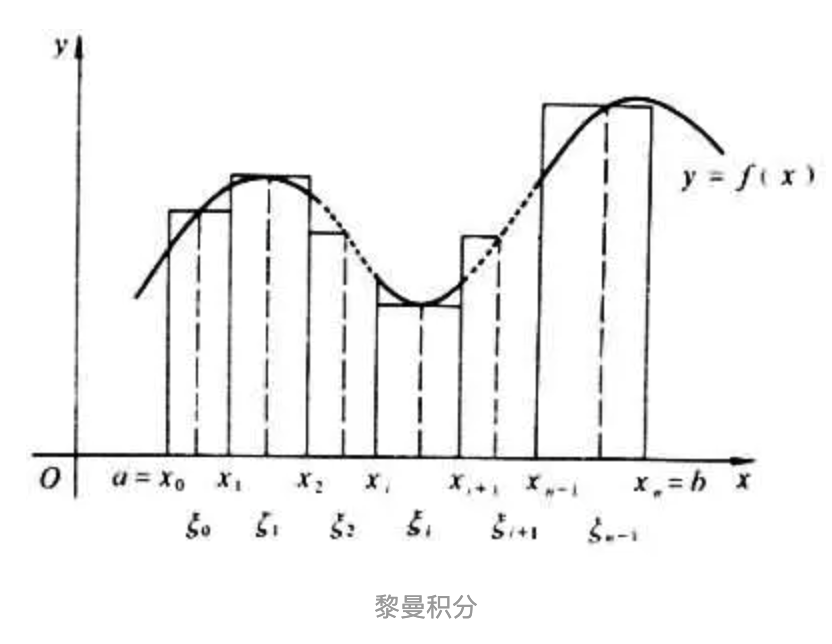
\includegraphics[width=9cm]{Riemanintegral.png}
	\end{figure}
\end{frame}

\begin{frame}{黎曼积分的缺点}
	\begin{itemize}[<+-|alert@+>]
		\item 一些很简单的函数不是黎曼可积的, 如{\rm Dirichlet} 函数:
		\[D(x):=\left\{\begin{array}{ll}
			1, & x \mbox{是有理数},\\
			0, & x \mbox{是无理数}.
		\end{array}\right.\]
		\item 需要一致收敛条件来保证函数积分与极限运算的次序交换, 即若 $f_n(x)$ 一致收敛且黎曼可积, 则
		\[\lim_{n\rightarrow\infty}\int_a^bf_n(x)dx=\int_a^b\lim_{n\rightarrow\infty}f_n(x)dx\]
		\item 黎曼可积函数空间不完备, 即存在黎曼可积函数列 $f_n(x)$ 逐点收敛到函数 $f(x)$, 但 $f(x)$ 不是黎曼可积.
	\end{itemize}
\end{frame}

\begin{frame}{黎曼积分的等价定义(I)}
	\begin{itemize}[<+-|alert@+>]
		\item 考虑函数 $f:[a,b]\mapsto \mathbb{R}$ 及分割 $\Delta$: $a=x_0<x_1<\cdots<x_n=b$, 并令 $|\Delta|:=\max_{1\leq i\leq n}|x_i-x_{i-1}|$ 以及
		\begin{align*}
			M_i(\Delta)&:=\sup_{x_{i-1}\leq x\leq x_i}f(x), \  m_i(\Delta):=\inf_{x_{i-1}\leq x\leq x_i}f(x),\\
			M(\Delta)&:=\sum_{i=0}^{n-1}M_i(x_{i+1}-x_i), \ m(\Delta):=\sum_{i=0}^{n-1}m_i(x_{i+1}-x_i).
		\end{align*}
		\item 上下积分:
		\begin{align*}
			\overline{\int_a^bf(x)dx}&:=\lim_{|\Delta|\rightarrow 0}M(\Delta)=\inf_{\Delta} M(\Delta), \\
			\underline{\int_a^bf(x)dx}&:=\lim_{|\Delta|\rightarrow 0}m(\Delta)=\sup_{\Delta} m(\Delta)
		\end{align*}
		\item  $f(x)$ 黎曼可积当且仅当上下积分相等, 即	$\overline{\int_a^bf(x)dx}=\underline{\int_a^bf(x)dx}$
	\end{itemize}
\end{frame}

\begin{frame}{黎曼积分的等价定义(II)}
	\begin{defi} (分段常值函数或阶梯函数) 函数 $f:[a,b]\mapsto \mathbb{R}$ 称为分段常值函数或阶梯函数, 如果区间 $[a,b]$ 存在一个有限区间分割 $I_1, I_2,\cdots, I_n$ 使得 $f(x)$ 在每个区间上 $I_i$ 上恒为常数 $c_i$, 即
		\[f(x)=\sum_{i=1}^{n}c_i1_{I_i}(x)\]
	\end{defi}
	\pause
	\begin{rmk}
		\begin{itemize}[<+-|alert@+>]
			\item 容易验证, $\sum_{i=1}^nc_i|I_i|$ 与分段常值函数或阶梯函数 $f(x)$ 表达形式中所选择的区间分割无关.%函数
			\item 我们记
			\[p.c.\int_a^bf(x)dx:=\sum_{i=1}^nc_i|I_i|\]
			并将其称为分段常值函数或阶梯函数 $f(x)$ 在 $[a,b]$ 上的积分.
		\end{itemize}
	\end{rmk}
\end{frame}
\begin{frame}{黎曼积分的等价定义(II)}
	\begin{defi} ({\rm Darboux integral} 达布积分) 设函数 $f:[a,b]\mapsto \mathbb{R}$ 为有界函数, 则
		\begin{itemize}[<+-|alert@+>]
			\item 称\[\underline{\int_a^b}f(x)dx:=\sup_{g\leq f,\  g\mbox{为阶梯函数}}p.c.\int_a^bg(x)dx\]
			为函数 $f(x)$ 在 $[a,b]$ 上的达布下积分;%$\underline{\int_a^b}f(x)dx$ 定义为
			\item 称\[\overline{\int_a^b}f(x)dx:=\inf_{h\geq f,\  h\mbox{为阶梯函数}}p.c.\int_a^bh(x)dx\]
			为函数 $f(x)$ 在 $[a,b]$ 上的达布上积分;
			\item 显然, $\underline{\int_a^b}f(x)dx\leq \overline{\int_a^b}f(x)dx$. 如果
			\[\underline{\int_a^b}f(x)dx=\overline{\int_a^b}f(x)dx,\]
			则称函数 $f(x)$ 在 $[a,b]$ 上达布可积.
		\end{itemize}
	\end{defi}

\end{frame}

\begin{frame}{黎曼积分的等价定义(II)}

	\begin{thm}
		设函数 $f:[a,b]\mapsto \mathbb{R}$ 为有界函数, 则函数 $f(x)$ 黎曼可积当且仅当函数 $f(x)$ 达布可积.
	\end{thm}

\end{frame}
\begin{frame}{黎曼积分的本质}

	\begin{itemize}[<+-|alert@+>]
		\item 黎曼积分思想源于古希腊的“穷竭法”.
		\begin{itemize}[<+-|alert@+>]
			\item 求圆的面积: 通过圆外切正 $n$ 边形和内接正 $n$ 边形, 来得到圆面积的上下界, 然后取极限发现上下界都相等, 从而得到圆的面积.
			\item 求函数 $f(x)$ 围成的面积: 把 $f(x)$ 与坐标轴围成的区域通过对定义域 $[a,b]$ 进行有限分割并利用分割小区间上函数 $f(x)$ 的最大最小值构造函数外接与函数内接长方形, 然后取分割的极限得到函数 $f(x)$ 围成的面积.
			\item 黎曼积分整个过程就是: 有限分割--近似求和--取极限.
		\end{itemize}
		\item 对函数\textcolor{cyan}{定义域进行有限区间分割}后近似求和取极限, 适用于连续函数, 即函数在小区间内振荡不明显, 但对然而对于振荡很厉害的函数, 哪怕分割很细, 在很细的区间内振荡依然很厉害(典型的例子是狄利克雷函数).
	\end{itemize}

\end{frame}
\subsection{{\rm Lebesgue} 积分}

\begin{frame}{{\rm Lebesgue} 积分基本思想}

	\begin{itemize}[<+-|alert@+>]
		\item 黎曼积分是对函数的定义域 $[a,b]$ 进行分割, 而{\rm Lebesgue} 积分则是对函数 $f(x)$ 的值域进行分割.
		\item  令 $l<L$ 分别为 $f(x)$ 在区间 $[a,b]$ 上的下确界与上确界, 考虑 $[l,L]$ 的分割 $\Delta_y$:
		\[l=l_0<l_1<l_2<\cdots<l_n=L\]

	\end{itemize}
	\pause
	\begin{figure}[htbp]
		\centering
		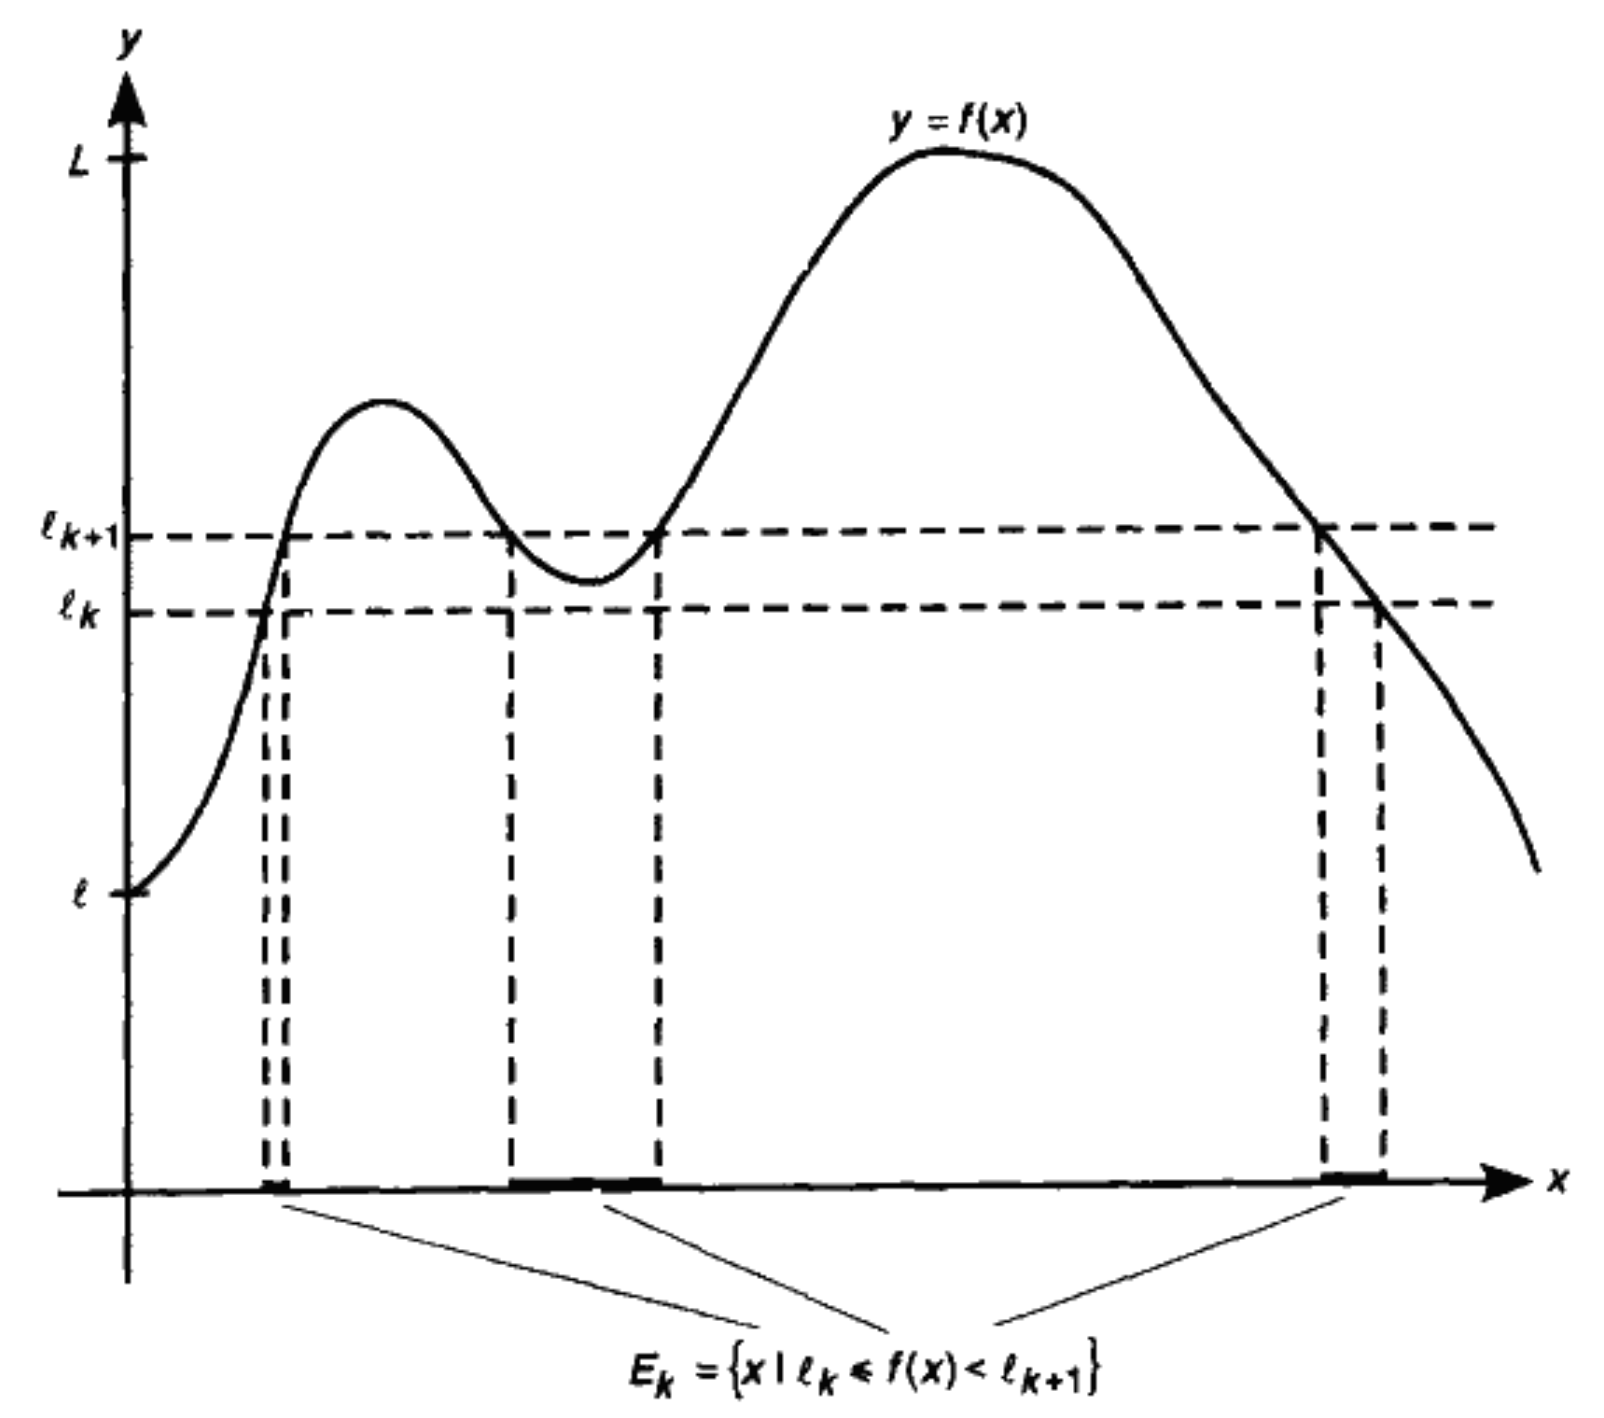
\includegraphics[width=9cm, height=4.8cm]{Lebesgueintegral.png}
	\end{figure}
\end{frame}
\begin{frame}{{\rm Lebesgue} 积分基本思想}

	\begin{itemize}[<+-|alert@+>]
		\item 令
		\begin{align*}
			|\Delta_y|&:=\max_{1\leq k\leq n}|l_k-l_{k-1}|, \\
			E_k&:=\{x:l_k\leq f(x)<l_{k+1}\}, k=0,1,\cdots, n-1,
		\end{align*}
		\item 显然
		\begin{align*}
			\sum_{k=0}^{n-1}l_k1_{E_k}(x)\leq f(x)<\sum_{k=0}^{n-1}l_{k+1}1_{E_k}(x), \forall x\in [a,b].
		\end{align*}
		因此, 相应的积分应保持上述不等关系, 即
		\begin{align*}
			\sum_{k=0}^{n-1}l_k\int_{a}^{b} 1_{E_k}(x)dx\leq \int_{a}^{b}f(x)dx<\sum_{k=0}^{n-1}l_{k+1}\int_{a}^{b}1_{E_k}(x)dx.
		\end{align*}
		\item 类似于黎曼积分的想法, 我们希望当值域分割$|\Delta_y|\to 0$时, 上述左右两端的极限存在且相等.
	\end{itemize}

\end{frame}


\begin{frame}{{\rm Lebesgue} 积分基本思想}

	\begin{itemize}[<+-|alert@+>]

		\item  若对每一个$E_k, k=0, \cdots, n-1$, 示性函数$1_{E_k}(x)$黎曼可积, 且$|\Delta_y|<\epsilon$, 则
		\begin{align*}
			\sum_{k=0}^{n-1}(l_{k+1}-l_k)\int_{a}^{b} 1_{E_k}(x)dx\leq \epsilon \sum_{k=0}^{n-1}\int_{a}^{b}1_{E_k}(x)dx=\epsilon (b-a).
		\end{align*}


		\item  若示性函数$1_{E_k}(x)$不是黎曼可积的,  如何定义:
		\begin{align*}
			m(E_k):=\int_{a}^{b}1_{E_k}(x)dx,
		\end{align*}
		也即集合$E_k$的测度$m(E_k)$如何定义?


		\item 若我们可以定义$m(E_k)$, 则我们可以类似于“黎曼和”一样, 我们构造“勒贝格和”, 用面积已知的一些区域逼近曲线下方的区域:
		\[\int_a^bf(x)dm:=\lim_{|\Delta_y|\rightarrow 0}\Big[\sum_{k=0}^{n-1}l_k\cdot m(E_k)\Big].\]
	\end{itemize}

\end{frame}
\begin{frame}{黎曼积与与{\rm Lebesgue} 积分的直观解释}

	\begin{itemize}[<+-|alert@+>]%微积分的历程 245-246
		\item 想像一位零售商,在一天结束营业时汇总今天的营业收入.
		\begin{itemize}
			\item 黎曼积分法: 从钱箱中依次取出现金累加计算获得总的营业收入;
			\item{\rm Lebesgue} 积分法: 先将钱箱中的现金按面值进行分类, 用面值乘以该面值现金的数量并累加求和获得总的营业收入.
		\end{itemize}
	\end{itemize}

\end{frame}




\subsection{集合的测度}

\begin{frame}
	\frametitle{如何测量集合大小}
	\begin{itemize}[<+-|alert@+>]
		\item  基数或势({\rm Cardinality}): 集合元素的个数;
		\item 称两个集合的基数相等, 如果两个集合之间存在一一映射;
		\item $A=\{2,4,6,\cdots,\}$与$B=\{1,2,3,4,\cdots\}$的基数是相等的;
		\item  基数或势的优缺点:
		\begin{itemize}[<+-|alert@+>]
			\item 在有限集上,基数还是很有用处的;
			\item 但对于无限集情形,这个度量显得过于粗糙,例如,实数集上任意两个区间的基数都是相同的;
		\end{itemize}
		\item 对于连续的集合,我们又有自然的``体积"的概念: \\
		一维空间:长度; 二维空间:面积; 三维空间:传统的体积;


	\end{itemize}
\end{frame}
\begin{frame}{可数集与不可数集}
\begin{itemize}[<+-|alert@+>]
	\item 称集合是可数(countable)的, 如果该集合和自然数集${\mathbf{N}}$的子集之间存在一一映射, 否则称该集合是不可数(uncountable)集.
	\item 可数集包括有限可数集和无穷可数集.
	\item 有限个可数集的并仍然是可数集,可数个可数集的并仍然是可数集.
	\item 两个可数集的笛卡尔积是可数集.
	\item 实数区间 ${(0,1)}$ 是典型的不可数集.\pause

	假设 ${(0,1)}$ 可数, 其元素可以排列为 ${a_{1}, a_{2}, a_{3}, \cdots}$. 注意到 ${(0,1)}$ 中的元素 ${a_{n}}$ 可以表示为
	\[
	a_{n}=0. a_{n}^{(1)} a_{n}^{(2)} a_{n}^{(3)} \cdots=\sum_{k=1}^{\infty} a_{n}^{(k)} 10^{-k}
	\]
	\pause

	构造 ${x=0.x_{1} x_{2} x_{3} \cdots}$, 其中, 对任意的 ${k}$, 取 ${x_{k} \neq a_{k}^{(k)}}$. \pause 显然, $x \neq a_{k}$, $\forall k \in \mathbf{N}$,矛盾.故 ${(0,1)}$ 是不可数集合. 由于
	\[
	f(x)=-\cot (\pi x):(0,1) \rightarrow(-\infty, \infty)
	\]

	是一一映射, 立刻得到 ${\mathbf{R}}$ 也是不可数集. %${\mathbf{R}}$ 是最典型、最重要的不可数集.
\end{itemize}

\end{frame}


\begin{frame}
	\frametitle{集合的测度}
	\begin{itemize}[<+-|alert@+>]
		\item 对于集合大小, 我们希望定义另外的度量标准:测度.
		\begin{itemize}[<+-|alert@+>]
			\item 希望定义一个测度来测量集合的大小,能够处理各种情况,包括有限集、无限集甚至是各种抽象的集合;
			\item 希望在某些特定的情况下,和我们熟知的度量相容:比如区间的长度,区域的面积,空间的体积等度量相容;
			\item 希望具有常见度量的一些性质:可加性.
		\end{itemize}
		\item 如此一来, 设计一个测度就好像变成了制造一把尺子(或者量筒:多维情形).
		\item 尺子有其适用范围:用一个普通米尺来测量地球的半径估计会很有困难,或者用它去测量原子的半径也是不可能的.
		\item 测度的适用范围在测度论里同样重要:在定义一个测度的时候,我们需要同时定义哪些集合是“可测的"({\rm measurable}) -- 也就是可以用这个测度来衡量.
	\end{itemize}
\end{frame}
\subsection{测度的构造}
\begin{frame}
	\frametitle{区间、矩形、基本集及其测度}
	\begin{itemize}[<+-|alert@+>]
		\item 区间 $I\subset\mathbb{R}$ : $[a,b],\  [a,b),\  (a,b), \cdots$;
		%		\item 矩形 $B\subset\mathbb{R}^d$: $[a,b]\times[c,d],\  [a,b]\times [c,d), \cdots$;
		%		\item 方体 $B\subset\mathbb{R}^d$:
		\item 矩形 $B\subset\mathbb{R}^d$: $B:=I_1\times \cdots\times I_d$, 其中$I_i$ 为区间;
		\item 矩形的测度: $|B|:=|I_1|\times|I_2|\times\cdots\times|I_d|$
		\item 基本集 $E\subset\mathbb{R}^d$: 能够表示为有限个矩形的并的集合;
		\begin{itemize}[<+-|alert@+>]
			\item 更进一步, 可以证明基本集一定可以表示为有限个不相交矩形的并, 即
			\[E=\cup_{i=1}^kB_i, \mbox{其中} B_i, i=1,\cdots, k, \mbox{为矩形且互不相交};\]
			\item 我们将 $m(E):=|B_1|+|B_2|+\cdots+|B_k|$ 称为基本集 $E$ 的基本测度.
		\end{itemize}
	\end{itemize}
\end{frame}
\begin{frame}
	\frametitle{约当测度({\rm Jordan Measure})}
	\begin{defi}
		(约当测度) 令 $E$ 为 $\mathbb{R}^d$ 的有界子集.
		\begin{itemize}
			\item 称
			\[m_{*,J}(E):=\sup_{A\subset E, A\mbox{为基本集}}m(A)\]
			为约当内测度;
			\item 称
			\[m^{*,J}(E):=\inf_{A\supset E, A\mbox{为基本集}}m(A)\]
			为约当外测度;
			\item 称 $E$ 为约当可测的, 如果 $m_{*,J}(E)=m^{*,J}(E)$. 此时称 $m(E):=m_{*,J}(E)=m^{*,J}(E)$ 为集合 $E$ 的约当测度.
		\end{itemize}
	\end{defi}
\end{frame}
\begin{frame}
	\frametitle{约当测度的优缺点}
	设 $E,\  F\subset\mathbb{R}^d$ 为约当可测集, 则
	\begin{itemize}[<+-|alert@+>]
		\item $E\cup F,\  E\cap F,\  E\backslash F,\  E\Delta F$ 均为约当可测集;
		\item 非负性: $m(E)\geq 0$;
		\item 有限可加性: 如果 $E, F$ 不相交, 则 $m(E\cup F)=m(E)+m(F)$;
		\item 平称不变性: $m(x+E)=m(E)$;
		\item $E_i, i=1,2,\cdots$ 约当可测, 但 $\cup_{i=1}^\infty E_i, \  \cap_{i=1}^\infty E_i$ 不一定约当可测
	\end{itemize}
\end{frame}

\begin{frame}{{\rm Riemann }积分与{\rm Jordan} 测度之间的联系}
\begin{thm}({\rm Riemann }积分与{\rm Jordan} 测度之间的联系)
	\begin{itemize}
		\item  如果 $E$ 是区间 $[a,b]$ 上的{\rm Jordan} 可测集, 则示性函数
		\begin{align*}
			1_{E}(x):=\left\{\begin{array}{ll}
				1, & x\in E \\ 0, & x\notin E \end{array}\right.
		\end{align*}
		是{\rm Riemann } 可积的且 $\int_{a}^b{1}_{E}(x) \, dx=m(E)$.
		\item  设 $[a,b]$ 为一区间, $f:[a,b]\rightarrow \mathbb{R}$ 为一有界函数, 则 $f$ 是{\rm Riemann }可积当且仅当
		\begin{align}
			E_+ &:=\{(x,t):x\in[a,b], 0\leq f(x)\leq t\}\\ E_-&:=\{(x,t):x\in[a,b], f(x)\leq t\leq 0\}
		\end{align}
		在 $\mathbb{R}^2$ 上是{\rm Jordan} 可测的, 且有
		$$\int_{a}^b f(x)  \, dx=m_{2}(E_{+})-m_{2}(E_{-}) $$
		此处的 $m_{2}$ 表示二维{\rm Jordan}  测度.
	\end{itemize}

\end{thm}
\end{frame}




\begin{frame}
	\frametitle{{\rm Lebesgue}测度}

	\begin{itemize}[<+-|alert@+>]
		\item{\rm Lebesgue}外测度$m^*(E)$:
		\[m^*(E):=\inf_{\cup_{i=1}^\infty B_i\supset E, B_i, i\geq 1, \mbox{为矩形}}\sum_{i=1}^\infty |B_i|\]
		\item 显然, $m^*(E)\leq m^{*,J}(E)$, 且存在$E\subset\mathbb{R}^d$使得不等号严格成立;
		\item{\rm Lebesgue}可测集的卡拉西奥多里({\rm Carath{\'e}odory})准则:\pause
		\vspace{0.4cm}

		称$E\subset\mathbb{R}^d$为{\rm Lebesgue}可测集, 如果对任意的$S\subset\mathbb{R}^d$均有
		\[m^*(S)=m^*(S\cap E)+m^*(S\backslash E),\]
		并称$m(E):=m^*(E)$为集合$E$的\textcolor{cyan}{{\rm Lebesgue}测度}.
	\end{itemize}
\end{frame}

\begin{frame}
	\frametitle{{\rm Lebesgue}可测集的代数结构}
	\begin{defi}\textcolor{cyan}{(事件或集合的{\rm Borel} 运算)}
		我们将对所给出的一些事件或集合所作的各种 (有限次或可列次) 取余、取交和取并运算以及它们的混合运算都称为 \textcolor{cyan}{事件或集合的{\rm Borel} 运算}。
	\end{defi}
\vspace{0.3cm}

	\pause
	\begin{defi}\textcolor{cyan}{($\sigma-$代数)} 设$\mathcal{F}$为$\mathbb{R}^d$的某些子集构成的集合类, 称$\mathcal{F}$为 $\mathbb{R}^d$上的$\sigma$-代数, 如果
		\begin{enumerate}[<+-|alert@+>][(1)]
			\item $\emptyset\in \mathcal{F}$;
			\item 若$A\in \mathcal{F}$, 则 $\overline{A}:=\mathbb{R}^d-A\in \mathcal{F}$;
			\item 若$A_i\in \mathcal{F}, i=1, 2,\cdots,$, 则$\cup_{i=1}^{\infty}A_i\in \mathcal{F}$.
		\end{enumerate}
	\end{defi}

	\vspace{0.3cm}
\pause
\begin{prop}
  在$\mathbb{R}^d$上的Lebesgue可测集具有以下性质:
  \begin{itemize}[<+-|alert@+>]
	\item 若$E,\  F\subset\mathbb{R}^d$ {\rm Lebesgue}可测, 则$E\cup F,\  E\cap F,\  E\backslash F,\  E\Delta F$ 均{\rm Lebesgue}可测;
	\item 若$E_i, i\geq 1$,{\rm Lebesgue}可测, 则$\cup_{i=1}^\infty E_i, \  \cap_{i=1}^\infty E_i$ 也{\rm Lebesgue}可测.
\end{itemize}
\end{prop}


\end{frame}


\begin{frame}
	\frametitle{{\rm Lebesgue}测度的性质}


	\begin{itemize}[<+-|alert@+>]
		\item 非负性: $m(E)\geq 0$;
		\item $m(\emptyset)=0$;
		\item 可列可加性: 如果 $E_i, i\geq 1 $ 互不相交且{\rm Lebesgue}可测, 则 \[m(\cup_{i=1}^\infty E_i)=\sum_{i=1}^\infty m(E_i);\]
		\item 平移不变性: $m(x+E)=m(E)$;
		\item 存在$F\subset\mathbb{R}^d$不{\rm Lebesgue}可测.

	\end{itemize}
\end{frame}









\begin{frame}
	\frametitle{不可测集}
	\textcolor{cyan}{巴拿赫-塔斯基分球悖论({\rm Banach-Tarski Paradox})}

	\qquad   将一个三维的半径为 $1$ 的实心球用某种巧妙方法分成五等分(五等分的意思是,把其中一份旋转平移后可以和另外一份重合), 然后把这五个分块旋转平移后,可以组合成两个半径为 $1$ 的实心球.

	\begin{figure}[htbp]
		\centering
		
\includegraphics[width=9cm]{fenqiu.jpg}
	\end{figure}
	\pause
	\textcolor{cyan}{选择公理({\rm Axiom of Choice})}:  任意一组(可能有不可数无限个)非空集合,我们都可以从每个集合挑出一个元素.
\end{frame}

\begin{frame}
	\frametitle{巴拿赫-塔斯基分球悖论的启示}
	\begin{itemize}[<+-|alert@+>]
		\item  在$\Omega=\mathbb{R}^3$时, 无法构造出一个测度既与常见的体积度量相容且具有平移不变性,又可以度量$\mathbb{R}^3$的任一子集;
		\item 类似的, 在$\Omega=\mathbb{R}$ 时,同样无法构造出一个测度既与常见的长度度量相容且具有平移不变性,又可以度量$\mathbb{R}$的任一子集; (\tc{不可测集构造详见教材第33-34页2.4节``不可测集".})
		\item 因此,对于可测空间$(\Omega,\mathcal{F})$中的$\mathcal{F}$通常为$\Omega$的某些子集构成的$\sigma$代数,而不一定是$\Omega$的所有子集构成的集类.

	\end{itemize}
\end{frame}

\begin{frame}
	\frametitle{ 由{\rm Lebesgue}测度到一般抽象测度}
	\begin{itemize}[<+-|alert@+>]
		\item 要度量集合元素的全体: $\Omega$
		\item 测度的适用范围(定义域): $\mathcal{F}:=\{A\subset \Omega:A\mbox{可测}\}$, 通常要求$\mathcal{F}$为$\sigma$-代数
		\item 通常称$(\Omega, \mathcal{F})$为可测空间
		\item 测度的定义: 称定义在$\mathcal{F}$的集函数$\mu(\cdot)$为测度, 如果
		\begin{enumerate}[<+-|alert@+>][(1)]
			\item $\mu(A)\ge 0, \forall A\in \mathcal{F}$;
			\item $\mu(\emptyset)=0$;
			\item $\mu$具有可列可加性: 若$A=\cup_{i=1}^{\infty}A_i$, 其中$A, A_i\in \mathcal{F}$,  且$i\neq j$时, $A_i\cap A_j=\emptyset$,  则
			\begin{eqnarray*}
				\mu(\cup_{i=1}^{\infty}A_i)=\sum_{i=1}^{\infty}\mu(A_i)
			\end{eqnarray*}

		\end{enumerate}
		\item  称$(\Omega,\mathcal{F},\mu)$为测度空间.
	\end{itemize}

\end{frame}

\subsection{概率与测度}


% \begin{frame}
% 	\frametitle{事件域或$\sigma$-代数}

% 	\begin{defi}\textcolor{cyan}{($\sigma-$代数)} 设$\mathcal{F}$为$\Omega$的某些子集构成的集合类, 称$\mathcal{F}$为 $\Omega$上的$\sigma$-代数(或事件域), 如果
% 		\begin{enumerate}[<+-|alert@+>][(1)]
% 			\item $\Omega\in \mathcal{F}$;
% 			\item 若$A\in \mathcal{F}$, 则 $\overline{A}:=\Omega-A\in \mathcal{F}$;
% 			\item 若$A_i\in \mathcal{F}, i=1, 2,\cdots,$, 则$\cup_{i=1}^{\infty}A_i\in \mathcal{F}$.
% 		\end{enumerate}
% 	\end{defi}

% \end{frame}

% \begin{frame}
% 	\frametitle{常见的事件域}
% 	\begin{itemize}[<+-|alert@+>]
% 		\item 若$\Omega=\{\omega_1,\omega_2\}$: 记$A=\{\omega_1\}, \overline{A}=\{\omega_2\}$, 则 $\mathcal{F}:=\{\emptyset, A,\overline{A}, \Omega\}$为事件域;
% 		\item  若$\Omega=\{\omega_1,\omega_2,\cdots,\omega_n\}$: 则 $\mathcal{F}:=\{A:A\subset \Omega\}$为事件域;
% 		\item 若$\Omega=(-\infty, +\infty)$: 记$\mathcal{P}=\{(-\infty, x):-\infty <x<+\infty\}$, 则 $\mathcal{F}=\mathcal{B}(\mathbb{R}):=\sigma(\mathcal{P})$为事件域.
% 	\end{itemize}
% \end{frame}





\begin{frame}
	\frametitle{概率与测度}
	\begin{itemize}[<+-|alert@+>]
		\item \textcolor{red}{$\Omega$:}  \textcolor{cyan}{概率论中的样本空间对应于测度中要度量的集合所包含元素的全体}
		\item \textcolor{red}{$\mathcal{F}$:} 事件域, 即某些随机事件组成的集合, 通常要求其为$\sigma$-代数;
		\begin{itemize}
			\item 注意到随机事件是随机试验中我们所关心的可能出现的结果, 它由一个或若干个基本事件组成, 因此事件是样本空间的子集, 从而事件域为样本空间的某些子集构成的集合;
			\item \textcolor{cyan}{概率论中的事件域对应于测度中要度量的集合全体即可测集的概念}
		\end{itemize}
		\item \textcolor{red}{$(\Omega,\mathcal{F})$:}可测空间
	\end{itemize}

\end{frame}


\begin{frame}
	\frametitle{概率的公理化定义}

	\begin{defi}\textcolor{cyan}{(概率的公理化定义)} 设$\Omega$为样本空间, $\mathcal{F}$为$\Omega$的某些子集组成的$\sigma$-代数(事件域), 若定义在$\mathcal{F}$上的集函数$P(\cdot)$满足
		\begin{enumerate}[<+-|alert@+>][(1)]
			\item 非负性: $P(A)\geq 0$;
			\item 正则性: $P(\Omega)=1\textcolor{red}{\Rightarrow P(\emptyset)=0 (\mbox{结合可列可加性})}$;
			\item 可列可加性: 若$A_i,i=1,2,\cdots$ 互不相交, 则
			\[P(\cup_{i=1}^\infty A_i)=\sum_{i=1}^\infty P(A_i).\]
		\end{enumerate}
		\pause
		\vspace{-0.5cm}则称$P$为$(\Omega,\mathcal{F})$上的概率测度,简称概率,称$(\Omega,\mathcal{F},P)$为概率空间.
	\end{defi}
\end{frame}

\begin{frame}
	\frametitle{关于概率的几个注记}
	% \vspace{-0.3cm}
	\begin{itemize}[<+-|alert@+>]
		\item 从概率的定义可以看出, 概率是全集度量为 $1$ 的测度;
		\item \tc{概率与我们熟知的度量(长度,面积,体积,质量)相比,本质上没有太大的区别},只不过概率是用来衡量随机事件发生可能性大小的一种度量, 其在全集上的度量为 $1$;
		\item 同一随机试验得到的可测空间$(\Omega,\mathcal{F})$, 可定义不同的概率.
		\begin{itemize}[<+-|alert@+>]
			\item 对于抛一枚硬币这一随机试验,
			\begin{eqnarray*}
				\Omega=\{\mbox{正,反}\}, \mbox{ 选取} \mathcal{F}=\{\emptyset, \{\mbox{正}\}, \{\mbox{反}\}, \Omega\};
			\end{eqnarray*}
			\item 我们可以构造概率$P_1(\cdot)$:
			\[P_1(\emptyset)=0, P_1(\{\mbox{正}\})=1/2,  P_1(\{\mbox{反}\})=1/2,  P_1(\Omega)=1;\]
			\item 也可以构造概率$P_2(\cdot)$: 其中$p+q=1$,
			\[P_2(\emptyset)=0, P_2(\{\mbox{正}\})=p,  P_2(\{\mbox{反}\})=q,  P_1(\Omega)=1.\]
		\end{itemize}

	\end{itemize}
\end{frame}


 %\section{概率简介}
\title[概率论]{第五讲:概率的公理化体系}
%\author[张鑫 {\rm Email: xzhangseu@seu.edu.cn} ]{\large 张 鑫}
\institute[东南大学数学学院]{\large \textrm{Email: xzhangseu@seu.edu.cn} \\ \quad  \\
	\large 东南大学 \ quad 数学学院 \\
	\vspace{0.3cm}
	%\trc{公共邮箱: \textrm{zy.prob@qq.com}\\
	%\hspace{-1.7cm}  密 \ qquad 码: \textrm{seu!prob}}
}
\date{}



{\setbeamertemplate{footline}{}
	\begin{frame}
		\titlepage
	\end{frame}
}

\subsection{概率论的公理化体系}
%\subsection{事件 $\sigma$ 域或 $\sigma$- 代数}

\begin{frame}{代数(algebra)或域(field)}
\begin{defi}\textcolor{cyan}{(集合的代数 (algebra))}  设${\mathcal{A}}$ 是由 ${\Omega}$ 的某些子集所构成的集合类, 称${\mathcal{A}}$为集合 ${\Omega}$ 上的代数, 如果,
	\begin{enumerate}[<+-|alert@+>]
		\item ${\Omega \in \mathcal{A}, \varnothing \in \mathcal{A}}$;
		\item 若 ${A \in \mathcal{A}}$, 则 $\overline{A}:=\Omega-A\in \mathcal{A}$;
		\item 若${A, B \in \mathcal{A}}$, 则 $A \cup B \in \mathcal{A}.$
	\end{enumerate}
\end{defi}

\pause

\begin{exam}
	设 ${\Omega=\{a, b, c, d\}}$, 则集族 ${\mathcal{A}=\{\varnothing, \Omega,\{a\},\{b, c, d\}\}}$ 是代数.
\end{exam}

\pause
\begin{exam}
	(有限集上的代数) 设 ${\Omega}$ 为有限集, 则集族 ${2^{\Omega}}$ (即 ${\Omega}$ 的所有子集构成的集合) 是代数. 例如, 当 ${\Omega=\{a, b, c\}}$ 时,
	\[
	\mathcal{A}=\{\varnothing, \Omega,\{a\},\{b\},\{c\},\{a, b\},\{b, c\},\{a, c\},\{a, b, c\}\}
	\]
	是代数.
\end{exam}

\pause
\begin{rmk}
	\begin{itemize}[<+-|alert@+>]
		\item 代数是"集合的集合",即其本身是集合, 其中的元素仍然是集合. %有时也称这种集合组成的集合为集族 (set class).
		\item 代数对于集合的求补、有限交和有限并运算封闭。
		\item 由于代数仅对集合的有限交并封闭,若样本空间 ${\Omega}$ 是无限集, 将会导致它将无法包含一些重要的集合 (特别是无限集合).
		\item 有必要对代数定义进行延伸, 加强其表达能力.
	\end{itemize}


\end{rmk}




\end{frame}






\begin{frame}
	\frametitle{事件 $\sigma$ 域定义及其性质}

	\begin{defi}\textcolor{cyan}{(事件 $\sigma$ 域或 $\sigma$- 代数)} 设 $\mathcal{F}$ 为 $\Omega$ 的某些子集构成的集合类,称 $\mathcal{F}$ 为 $\Omega$ 上的事件 $\sigma$ 域或 $\sigma$- 代数,如果
		\begin{enumerate}[<+-|alert@+>]
			\item $\Omega\in \mathcal{F}$;
			\item 若 $E\in \mathcal{F}$, 则 $\overline{E}:=\Omega-E\in \mathcal{F}$;
			\item 若 $E_i\in \mathcal{F}, i=1, 2,\cdots,$ 则 $\cup_{i=1}^{\infty} E_i\in \mathcal{F}$.
		\end{enumerate}
	\end{defi}
	\pause

	\begin{thm} 若 $\mathcal{F}$ 为 $\Omega$ 上的 $\sigma$-代数,则
		\begin{itemize}[<+-|alert@+>]
			\item $\emptyset\in \mathcal{F}$;
			\item 若 $E_k\in \mathcal{F}, k=1,2,\cdots,$ 则 $\cap_{k=1}^\infty E_k\in \mathcal{F}$;
			\item 若 $E_1,\cdots, E_n\in \mathcal{F}$, 则 $\cap_{k=1}^nE_k\in \mathcal{F}$ 且 $\cup_{k=1}^nE_k\in \mathcal{F}$;

			\item 若 $E_1,E_2\in\mathcal{F}$, 则 $E_1-E_2\in \mathcal{F}$.
		\end{itemize}
	\end{thm}
\end{frame}

\begin{frame}{几个例子}
	\begin{exam}\textcolor{cyan}{(代数而非 ${\sigma}$-代数)} 设 ${\Omega}$ 是无限集合, 集族 ${\mathcal{A} \subset 2^{\Omega}}$ ,满足
		\[
		A \in \mathcal{A} \Longleftrightarrow \# A<\infty \text { 或  }  \# \overline{A}<\infty \text {, }
		\]

		即 ${\mathcal{A}}$ 中的集合或者自身是有限集,或者其补集是有限集.
		容易验证, ${\mathcal{A}}$ 是代数, 但不是 ${\sigma}$-代数.
	\end{exam}
\pause
\vspace{0.1cm}
\begin{exam}
	\textcolor{cyan}{(可数集上 ${\sigma}$-代数)} 设样本空间${\Omega}$为可数集, ${\mathcal{F}}$ 为其上的 ${\sigma}$-代数, 且 ${\forall a \in \Omega}$, 有 ${\{a\} \in \mathcal{F}}$, 则${\forall A \subset \Omega}$, 有${A \in \mathcal{F}}$.
\end{exam}

\begin{exam}设${\mathcal{F}}$为实数集${\mathbf{R}}$上的${\sigma}$-代数. 若对${\forall x\in\mathbf{R}}$,都有${(-\infty,x]\in\mathcal{F}}$, 则${\mathcal{F}}$包含${\mathbf{R}}$上的任意区间.
\end{exam}
\pause

\vspace{0.1cm}

\begin{proof}
	仅以${[a,b)}$为例. 注意到:%由式${(2-12)}$,
	\begin{align*}
		(-\infty, a)&=\bigcup_{k=1}^{\infty}\left(-\infty, a-\frac{1}{k}\right] \in \mathcal{F},  \pause \quad (x, \infty)=\overline{(-\infty, x]} \in \mathcal{F},  \forall x \pause \\
		[b, \infty)&=\bigcap_{k=1}^{\infty}\left(b-\frac{1}{k}, \infty\right) \in \mathcal{F}  \pause \quad	 	[a, b)=\overline{(-\infty, a) \cup [b, \infty)} \in \mathcal{F}
	\end{align*}


\end{proof}



\end{frame}





\begin{frame}
	\frametitle{$\sigma$-代数例子及如何构造}
	\begin{itemize}[<+-|alert@+>]
		\item $\mathcal{F}:=\{\emptyset, \Omega\}$;
		\item $\mathcal{F}:=\{A:A\subset \Omega\}$;
		\item $\mathcal{F}:=\{\emptyset, A, \bar{A}, \Omega\}$;
		\item 如何由 $\{A,B\}$(假设 $A,B$ 为非平凡事件,互不包含且不互为对立事件) 扩充成事件 $\sigma$ 域?
	\end{itemize}
\end{frame}

% \begin{frame}{{\rm Borel} 运算与生成 $\sigma$-代数}
% 	% \begin{defi}\textcolor{cyan}{(事件或集合的{\rm Borel} 运算)}
% 	% 	我们将对所给出的一些事件或集合所作的各种 (有限次或可列次) 取余、取交和取并运算以及它们的混合运算都称为 \textcolor{cyan}{事件或集合的{\rm Borel} 运算}。
% 	% \end{defi}
% 	%\pause
% 	\vspace{0.5cm}
% 	\begin{prop}\
% 		$\sigma$ 域就是一切可能的 Borel 运算之下封闭的集合 ($\Omega$ 的子集) 类。
% 	\end{prop}
% 	\pause
% 	\vspace{0.5cm}
% 	\begin{defi}\
% 		如果 $\mathcal{C}$ 是 $\Omega$ 的一个子集类,那么 $\mathcal{C}$ 中的集合做一切可能的 Borel 运算所得到的 $\sigma$ 域 $\mathcal{F}$ 称为由 $\mathcal{C}$ 生成的 $\sigma$ 域,记作 $\mathcal{F}=\sigma (\mathcal{C})$。
% 	\end{defi}
% 	%%	~\
% 	%%	\begin{thm}
% 	%%		实直线上的如下三种 $\sigma$ 域相同,都是一维 Borel 域 $\mathcal{B}^1$:
% 	%%		\begin{enumerate}
% 	%%			\item 由全体有界开区间构成的类所生成的 $\sigma$ 域;
% 	%%			\item 由子集类 $\left\{(-\infty,x)|x\in\mathbb{R}\right\}$ 所生成的 $\sigma$ 域;
% 	%%			\item 由全体开集和闭集构成的类所生成的 $\sigma$ 域。
% 	%%		\end{enumerate}
% 	%%	\end{thm}
% \end{frame}

\begin{frame}
	\frametitle{最小(生成)$\sigma$-代数}
	\begin{thm}
		假设 $\mathcal{C}$ 为 $\Omega$ 的子集组成的非空集类,则存在唯一 $\sigma$-代数 $\mathcal{C}_0$ 使得:
		\begin{enumerate}[<+-|alert@+>][(1)]
			\item $\mathcal{C}\subset \mathcal{C}_0$;
			\item 若 $\mathcal{G}$ 为任一 $\sigma$-代数,且 $\mathcal{C}\subset \mathcal{G}$, 则 $\mathcal{C}_0\subset \mathcal{G}$.
		\end{enumerate}
	\end{thm}

	\pause
	\zheng
	\begin{itemize}[<+-|alert@+>]
		\item 若 $\mathcal{F}_t, t\in T$ 为一族 $\sigma$-代数,则 $\cap_{t\in T}\mathcal{F}_t$ 仍为 $\sigma$-代数;
		\item 令 $C^{\#}:=\{\mathcal{B}:\mathcal{B}\mbox{为}\sigma-\mbox{代数}, \mathcal{C}\subset \mathcal{B}\}$;

		\item 令 $\mathcal{C}_0:=\cap_{\mathcal{B}\in C^{\#}}\mathcal{B}$, 则易证 $\mathcal{C}_0$ 即为定理所求之 $\sigma$-代数.
	\end{itemize}

	\pause
	\begin{rmk}
		\begin{itemize}[<+-|alert@+>]
			\item $\mathcal{C}_0:=\cap_{\mathcal{B}\in C^{\#}}\mathcal{B}$ 是包含集类 $\mathcal{C}$ 的最小 $\sigma$-代数;
			\item 一般也称 $\mathcal{C}_0$ 为集类 $\mathcal{C}$ 的生成 $\sigma$-代数,后面我们常用 $\sigma (\mathcal{C})$ 表示 $\mathcal{C}_0$.
		\end{itemize}
	\end{rmk}
\end{frame}
\begin{frame}
	\frametitle{实直线上的 $\sigma$- 域}
	\begin{exam}
		令 $\Omega:=\mathbb{R}$, 考虑
		\[\mathcal{A}_1=\{(-\infty, x)|x\in\mathbb{R}\}, \  \mathcal{A}_2=\{(a, b)|-\infty<a<b<\infty\},\]
		则 $\sigma (\mathcal{A}_1)=\sigma (\mathcal{A}_2)$
	\end{exam}

	\pause
	\jieda  注意到,对任意实数 $x$, 均有
	\[(-\infty, x)=\cup_{n=1}^\infty(x-n,x).\]
	\pause 因此 $(-\infty, x)\in\sigma (\mathcal{A}_2)$, \pause 从而 $\mathcal{A}_1\subset \sigma (\mathcal{A}_2)$, \pause 进而可得 $\sigma (\mathcal{A}_1)\subset\sigma (\mathcal{A}_2)$.

	\pause 反之,注意到 $[a,b)=(-\infty, b)-(-\infty,a)\in\sigma (\mathcal{A}_1)$ 以及
	\[\{a\}=\cap_{n=1}^\infty[a,a+\dfrac{1}{n})\in\sigma(\mathcal{A}_1),\]
	\pause 因此,$(a,b)=[a,b)-\{a\}\in\sigma (\mathcal{A}_1)$, \pause 即 $\mathcal{A}_2\subset\sigma (\mathcal{A}_1)$, \pause 从而
	\[\sigma(\mathcal{A}_2)\subset \sigma(\mathcal{A}_1).\]
\end{frame}


\begin{frame}
	\frametitle{Borel 集}
	\begin{exam}
		设 $\Omega=\mathbb{R}$, 令
		\begin{eqnarray*}
			\mathcal{C}_1&=&\{(-\infty,x):-\infty<x<+\infty\}\\
			\mathcal{C}_2&=&\{(a,b]:-\infty\leq a\leq b<+\infty\}\\
			\mathcal{C}_3&=&\{[a,b]:-\infty< a\leq b<+\infty\}\\
			\mathcal{C}_4&=&\{[a,b):-\infty< a\leq b\leq+\infty\}\\
			\mathcal{C}_5&=&\{(a,b):-\infty\leq a\leq b\leq+\infty\}\\
			\mathcal{C}_6&=&\{A\subset\mathbb{R}:A\mbox{为开集}\}\\
			\mathcal{C}_7&=&\{A\subset\mathbb{R}:A\mbox{为闭集}\}
		\end{eqnarray*}
		则以上 7 个集类的生成 $\sigma$-代数均相同,称以上集类的生成 $\sigma$-代数中的元素为 Borel 集,并记作 $\mathcal{B}(\mathbb{R})$, 即
		\begin{eqnarray*}
			\sigma(\mathcal{C}_1)=\cdots=\sigma(\mathcal{C}_7):=\mathcal{B}(\mathbb{R}).
		\end{eqnarray*}

	\end{exam}
\end{frame}
%\begin{frame}
%	\frametitle{实直线上的 $\sigma$- 域}
%	\begin{thm}
%		实直线上的如下三种 $\sigma$ 域相同,都是一维 Borel 域 $\mathcal{B}^1$:
%			\begin{enumerate}
%				\item 由全体有界开区间构成的类所生成的 $\sigma$ 域;
%				\item 由子集类 $\left\{(-\infty,x)|x\in\mathbb{R}\right\}$ 所生成的 $\sigma$ 域;
%				\item 由全体开集和闭集构成的类所生成的 $\sigma$ 域。
%		\end{enumerate}
%	\end{thm}
%\end{frame}







\begin{frame}
	\frametitle{其他集类}
	\begin{defi}
	  设$\mathcal{C}$为$\Omega$的某些子集构成的非空集类,
	  \begin{itemize}[<+-|alert@+>]
	  \item 称$\mathcal{C}$为$\pi$类, 如果$\mathcal{C}$关于有限交运算封闭, 即
		\begin{eqnarray*}
		  A,B\in \mathcal{C}\Rightarrow A\cap B\in \mathcal{C};
		\end{eqnarray*}
	  \item 称$\mathcal{C}$为代数, 如果$\mathcal{C}$关于有限交与取余运算封闭, 即
		\begin{eqnarray*}
		  A,B\in \mathcal{C}\Rightarrow A\cap B\in \mathcal{C}, \bar{A}\in \mathcal{C};
		\end{eqnarray*}
	  \item 称$\mathcal{C}$为单调类, 如果$\mathcal{C}$关于单调极限运算封闭, 即
		\begin{eqnarray*}
		  A_n\in \mathcal{C}, A_n\uparrow A \mbox{ 或 } A_n\downarrow A \Rightarrow A\in \mathcal{C}
		\end{eqnarray*}
	  \item 称$\mathcal{C}$为$\lambda$类, 如果$\Omega\in \mathcal{C}$并且$\mathcal{C}$对真差运算及上升极限运算封闭, 即
		\begin{itemize}
		\item $\Omega\in \mathcal{C}$;
		\item $A, B\in \mathcal{C}, B\subset A\Rightarrow A-B\in \mathcal{C}$;
		\item $A_n\in \mathcal{C}, n\geq 1, A_n\uparrow A\Rightarrow A\in \mathcal{C}$
		\end{itemize}

	  \end{itemize}

	\end{defi}
  \end{frame}

  \begin{frame}
	\frametitle{集类之间的关系}
	\begin{thm}
	  设$\mathcal{C}$为$\Omega$的某些子集构成的非空集类,则
	  \begin{enumerate}
	  \item 若$\mathcal{C}$为$\sigma-$代数,则$\mathcal{C}$一定是:$\pi$类,代数,$\lambda$类,单调类;
	  \item 若$\mathcal{C}$既是代数又是单调类,则$\mathcal{C}$一定是$\sigma-$代数;
	  \item 若$\mathcal{C}$既是$\pi$类又是$\lambda$类,则$\mathcal{C}$一定是$\sigma-$代数.
	  \end{enumerate}

	\end{thm}

  \end{frame}
  \begin{frame}
	\frametitle{单调类定理}
	\begin{defi}
	  与生成$\sigma-$代数类似, 我们可以定义包含集类$\mathcal{C}$的最小单调类$m(\mathcal{C})$及最小$\lambda$类$\lambda(\mathcal{C})$, 分别称为由集类$\mathcal{C}$生成的单调类与$\lambda$类.
	\end{defi}
  \vspace{0.2cm}
  \pause
	\begin{thm}(单调类定理) 设$\mathcal{C},\mathcal{G}$为$\Omega$中的集类且$\mathcal{C}\subset \mathcal{G}$,则
	  \begin{enumerate}
	  \item 若$\mathcal{C}$为一代数,则$m(\mathcal{C})=\sigma(\mathcal{C})$;
	  \item 若$\mathcal{C}$为一$\pi$类,则$\lambda(\mathcal{C})=\sigma(\mathcal{\mathcal{C}})$;
	  \item 若$\mathcal{C}$为代数而$\mathcal{G}$为单调类, 则$\sigma(\mathcal{C})\subset \mathcal{G}$;
	  \item 若$\mathcal{C}$为$\pi$类而$\mathcal{G}$为$\lambda$类,则$\sigma(\mathcal{C})\subset \mathcal{G}$.
	  \end{enumerate}
	\end{thm}
  \end{frame}


  \begin{frame}
	\frametitle{如何应用单调类定理}
	\begin{itemize}[<+-|alert@+>]
	\item 问题: 如何证明某$\sigma-$代数$\mathcal{F}$中的所有元素都具有某种性质($P$)?
	\item 步骤:
	  \begin{itemize}[<+-|alert@+>]
	  \item $\mathcal{G}:=\{A\in \mathcal{F}: A\mbox{具有性质}(P)\}$;
	  \item 找到某一集类$\mathcal{C}$为代数或$\pi$类且具有以下性质:
		\begin{eqnarray*}
		  \mathcal{C}\subset \mathcal{G}, \quad  \sigma(\mathcal{C})=\mathcal{F};
		\end{eqnarray*}
	  \item 证明$\mathcal{G}$为单调类或$\lambda$类;
	  \item 由单调类定理可知:
		\begin{eqnarray*}
		  \mathcal{F}=\sigma(\mathcal{C})\subset \mathcal{G}\subset \mathcal{F}
		\end{eqnarray*}
   即
   \begin{eqnarray*}
	 \mathcal{G}=\mathcal{F}
   \end{eqnarray*}
  从而$\mathcal{F}$中所有的元素都具有某种性质(P).
	  \end{itemize}

	\end{itemize}
  \end{frame}

% \begin{frame}
% 	\frametitle{单调类定理应用举例}
% 	\begin{exam}
% 	  设$\mathcal{C}$为$\Omega$上的一$\pi$类,$\mu_1$及$\mu_2$为$\sigma(\mathcal{C})$上的两个概率测度. 若$\mu_1$与$\mu_2$限于$\mathcal{C}$一致, 则对任意的$A\in \sigma(\mathcal{C})$均有$\mu_1(A)=\mu_2(A)$.
% 	\end{exam}

% 	\zheng 证明思路如下:
% 	\begin{itemize}[<+-|alert@+>]
% 	\item 令$\mathcal{G}:=\{A\in \sigma(\mathcal{C}):\mu_1(A)=\mu_2(A)\}$;
% 	\item 注意到$\mathcal{C}$为$\pi$类且$\mathcal{C}\subset \mathcal{G}$,故只需证明$\mathcal{G}$为$\lambda$类即验证即
% 	  \begin{itemize}[<+-|alert@+>]
% 	  \item $\Omega\in \mathcal{G}$;
% 	  \item $A, B\in \mathcal{G}, B\subset A\Rightarrow A-B\in \mathcal{G}$;
% 	  \item $A_n\in \mathcal{G}, n\geq 1, A_n\uparrow A\Rightarrow A\in \mathcal{G}$
% 	  \end{itemize}
% 	\item 利用单调类定理可知$\mathcal{G}=\sigma(\mathcal{C})$
% 	\end{itemize}

%   \end{frame}



\subsection{概率的公理化定义与性质}
\begin{frame}
	\frametitle{概率的公理化定义}
	\begin{defi} 设 $\mathcal{F}$ 为样本空间 $\Omega$ 上的 $\sigma$-代数,如果定义在 $\mathcal{F}$ 上的集函数 $P (\cdot)$ 具有:
		\begin{enumerate}[<+-|alert@+>]
			\item 非负性: $P (A)\ge 0, \forall A\in \mathcal{F}$;
			\item 规范性: $P (\Omega)=1$;
			\item 可列可加性:对 $\mathcal{F}$ 中的任何两两互不相容事件列 $\{A_n\}$ 有
				\begin{eqnarray*}
					P(\cup_{n=1}^{\infty}A_n)=\sum_{n=1}^{\infty}P(A_n)
				\end{eqnarray*}
		\end{enumerate}
		\pause  则称 $P (\cdot)$ 为 $\mathcal{F}$ 上的概率测度,而 $P (A)$ 称为事件 $A$ 的概率,$(\Omega,\mathcal{F},P)$ 称为概率空间.

	\end{defi}
\end{frame}


\begin{frame}{如何定义概率}
\begin{itemize}[<+-|alert@+>]
	\item 概率定义在${\sigma-}$代数${\mathcal{F}}$上, 但是由于${\mathcal{F}}$中集合的复杂性, 直接对每个集合赋予概率存在困难;
	\item 首先在${\mathcal{F}}$的子族${\mathcal{A} \subset \mathcal{F}}$上定义概率(一般${\mathcal{A}}$中的集合较为简单), 然后再将其扩张到${\mathcal{F}}$上;%变得十分自然;
	\item 如何选择恰当的${\mathcal{A}}$, 使得${\mathcal{F}=\sigma(\mathcal{A})}$?%是通常的思路.
\end{itemize}




\end{frame}

\begin{frame}{扩张是否唯一?}
\begin{exam}
(\tc{有限集合上的概率}) 设样本空间${\Omega=\{a, b, c, d\}, \sigma}$-代数${\mathcal{F}}$由集族${\mathcal{A}}$生成, 即
	\[
	\mathcal{F}=\sigma(\mathcal{A}), \quad  \mathcal{A}=\{\{a\},\{a, b\},\{a, b, c\}, \Omega\}
	\]
\end{exam}
\pause

\begin{exam}
令$\Omega=\{a, b, c, d\}$, $\mathcal{F}=2^{\Omega}$, $\mathcal{A}=\{\{a, b\},\{a, c\},\{b, d\},\{c, d\}\}$.

\begin{itemize}[<+-|alert@+>]
	\item 容易看出,${\sigma(\mathcal{A})=2^{\Omega}}$;
	\item 定义${P_{1}}$和${P_{2}}$为
	{\small \begin{align*}
		P_{1}(\{a\})&=P_{1}(\{d\})=\frac{1}{6}, \quad  P_{1}(\{b\})=P_{1}(\{c\})=\frac{1}{3} \\
		P_{2}(\{a\})&=P_{2}(\{d\})=\frac{1}{3}, \quad  P_{2}(\{b\})=P_{2}(\{c\})=\frac{1}{6}
	\end{align*}}

	\item 显然, 它们并不相同, 但它们在${\mathcal{A}}$上却完全一致
	{\small \begin{align*}
		P_{1}(\{a, b\})&=\frac{1}{2}, P_{1}(\{a, c\})=\frac{1}{2}, P_{1}(\{b, d\})=\frac{1}{2}, P_{1}(\{c, d\})=\frac{1}{2}\\
		P_{2}(\{a, b\})&=\frac{1}{2}, P_{2}(\{a, c\})=\frac{1}{2}, P_{2}(\{b, d\})=\frac{1}{2}, P_{2}(\{c, d\})=\frac{1}{2}
	\end{align*}}
	%\item 存在两种概率${P_{1}}$和${P_{2}}$, 使得它们在${\mathcal{A}}$上取值相同, 但在${\mathcal{F}}$上的扩展却不一致.
\end{itemize}


\end{exam}



\end{frame}


\begin{frame}{概率扩张唯一性定理}
\begin{thm}(\tc{概率扩张的唯一性}) 给定样本空间${\Omega}$和其上的${\sigma}$-代数$\mathcal{F}$. 若
\begin{itemize}[<+-|alert@+>]
	\item $P_{1}$和${P_{2}}$是定义在${\mathcal{F}}$上的两个概率;
	\item 集族${\mathcal{A}}$关于交运算封闭, 且${\sigma(\mathcal{A})=\mathcal{F}}$;
	\item 对任意的$A\in \mathcal{A}$均有${P_{1}(A)=P_{2}(A)}$;
\end{itemize}\pause
则对任意的$A\in \mathcal{F}$一定有${P_{1}(A)=P_{2}(A)}$.
\end{thm}
\pause

\zheng 证明思路如下:
	\begin{itemize}[<+-|alert@+>]
	\item 令$\mathcal{G}:=\{A\in \sigma(\mathcal{A}):P_1(A)=P_2(A)\}$;
	\item 注意到$\mathcal{A}$为$\pi$类且$\mathcal{A}\subset \mathcal{G}$,故只需证明$\mathcal{G}$为$\lambda$类即验证即
	  \begin{itemize}[<+-|alert@+>]
	  \item $\Omega\in \mathcal{G}$;
	  \item $A, B\in \mathcal{G}, B\subset A\Rightarrow A-B\in \mathcal{G}$;
	  \item $A_n\in \mathcal{G}, n\geq 1, A_n\uparrow A\Rightarrow A\in \mathcal{G}$
	  \end{itemize}
	\item 利用单调类定理可知$\mathcal{G}=\sigma(\mathcal{A})$
	\end{itemize}


\end{frame}


\begin{frame}{(概率)测度扩张定理}
\begin{thm}(\tc{Carath{\'e}odory测度扩张定理}) 设$\Omega$为样本空间,$\mathcal{A}$为代数. %$\sigma(\mathcal{A})$为包含$\mathcal{A}$的最小$\sigma-$代数.
如果$P_{0}$为定义在$\mathcal{A}$上的概率, 且满足可数可加性, 那么存在唯一的定义在$\sigma(\mathcal{A})$上的概率$P$, 满足
	\[
	P(A)=P_{0}(A),  \quad \forall A \in \mathcal{A},
	\]
\end{thm}


\begin{rmk}
更一般的测度扩张定理详见测度论教材,如严加安院士的``测度论讲义"等.
\end{rmk}
\end{frame}

\begin{frame}{如何理解概率}
\begin{itemize}[<+-|alert@+>]
	\item 概率空间定义中的样本空间$\Omega$和概率$P$都很好理解,但是$\sigma$-代数$\mathcal{F}$的出现总是显得有些突兀.
	\item 概率是一个以事件(集合)为自变量的函数.
	\item 给定一个事件(集合), 概率函数即赋予它一个非负实数, 用以表示该事件(集合)的样本点在统计实验的结果中出现的可能性大小.
	\item 函数的基本概念中,"定义域" 占据重要位置. 概率函数也不例外.
	\item 函数的定义域中的数对``加减乘除"运算封闭. 类似的, 概率函数应对事件的``交差并补"等运算封闭.
	\item $\sigma$-代数$\mathcal{F}$本质上就是概率函数的 ``定义域", 对自变量(事件)的``交差并补"等运算封闭..
\end{itemize}




\end{frame}






\begin{frame}%[allowframebreaks,allowdisplaybreaks]
	\frametitle{概率测度的性质 I}
	\begin{thm}
		设 $(\Omega,\mathcal{F},P)$ 为一概率空间,则其上的概率 $P$ 具有如下性
		质:
		\begin{enumerate}[<+-|alert@+>]
			\item $P(\emptyset)=0$;
			\item 有限可加性:若 $A_1,\cdots, A_n$ 为 $\mathcal{F}$ 中两两互不相
			      容事件,则
			      \begin{eqnarray*}
				      P(\cup_{k=1}^n A_k)=\sum_{k=1}^nP(A_k)
			      \end{eqnarray*}
			\item 可减性:若 $A, B\in \mathcal{F}$ 且 $A\subset
				      B$, 则 $P (B-A)=P (B)-P (A)$;
			\item 单调性:若 $A, B\in \mathcal{F}$ 且 $A\subset B$,
			      则 $P (A)\leq P (B)$;
			\item $P(\bar{A})=1-P(A)$;
		\end{enumerate}
	\end{thm}
\end{frame}
\begin{frame}
	\frametitle{概率测度的性质 II}

	\begin{enumerate}[<+-|alert@+>]
		\setcounter{enumi}{5}

		\item 加法公式(容斥原理):对任意两个事件 $A,B$, 有
		      \begin{eqnarray}\label{eq:plusformulatwo}
			      P(A\cup B)=P(A)+P(B)-P(AB).
		      \end{eqnarray}
		      一般的,对任意 $n$ 个事件 $A_1,\cdots,A_n$, 有
		      {\small \begin{eqnarray}
			      \label{eq:plusformula}
			      P(\cup_{i=1}^nA_i)&=&\sum_{i=1}^nP(A_i)-\sum_{1\leq i<j\leq n}P(A_iA_j)+\sum_{1\leq i<j<k\leq n}P(A_iA_jA_k)\nonumber\\
			      && +\cdots+(-1)^{n-1}P(A_1A_2\cdots A_n).
		      \end{eqnarray}}
		\item 次可加性(Boole不等式):对任意两个事件 $A,B$, 有
		      \begin{eqnarray*}
			      P(A\cup B)\leq P(A)+P(B).
		      \end{eqnarray*}
		      一般的,对任意 $n$ 个事件 $A_1,\cdots,A_n$, 有
		     {\small  \begin{align*}
			      P(\cup_{i=1}^nA_i)&\leq \sum_{i=1}^nP(A_i).
		      \end{align*}}
	\end{enumerate}

\end{frame}

\begin{frame}
	\frametitle{概率测度的性质 III}

	\begin{enumerate}[<+-|alert@+>]
		\setcounter{enumi}{7}
		\item Bonferroni不等式:
		{\small \begin{align*}
			P(\cup_{i=1}^{n} A_{i}) &\geq \sum_{i=1}^{n} P(A_{i})-\sum_{1\leq i<j\leq n} P(A_{i} \cap A_{j}), \\
			P(\cup_{i=1}^nA_i)&\leq \sum_{i=1}^{n} P(A_{i})-\sum_{1\leq i<j\leq n} P(A_{i} \cap A_{j})+\sum_{1\leq i<j<k\leq n}P(A_i\cap A_j\cap A_k), \cdots.
		\end{align*}}
		\item 下连续性:
		      若 $A_n\in\mathcal{F}$ 且 $A_n\subset A_{n+1}, n=1,2,\cdots,$ 则
		      \begin{eqnarray*}
			      P(\cup_{n=1}^\infty A_n)=P(\lim_{n\rightarrow\infty}A_n)=\lim_{n\rightarrow\infty}P(A_n)
		      \end{eqnarray*}
		\item 上连续性:
		      若 $A_n\in\mathcal{F}$ 且 $A_n\supset A_{n+1}, n=1,2,\cdots,$ 则
		      \begin{eqnarray*}
			      P(\cap_{n=1}^\infty A_n)=P(\lim_{n\rightarrow\infty}A_n)=\lim_{n\rightarrow\infty}P(A_n)
		      \end{eqnarray*}
		\item 概率 $P$ 的可列可加性等价于 $P$ 有限可加且下连续.
	\end{enumerate}

	% \end{thm}
\end{frame}

\begin{frame}%[allowframebreaks]
	\frametitle{加法公式证明 I}
	% \begin{enumerate}[<+-|alert@+>]
	% \item ({\color{red} 加法公式的证明})
	注意到
	\begin{eqnarray*}
		A\cup B=A\cup (B-AB).
	\end{eqnarray*}
	\pause  故由概率的有限可加性及减法公式可得:
	\begin{eqnarray*} P(A\cup B)=P(A)+P(B)-P(AB).
	\end{eqnarray*}
	\pause 对于一般情形,可由归纳法证明。当 $n=2$ 时,\eqref{eq:plusformula} 式即为
	\eqref{eq:plusformulatwo} 式。设 \eqref{eq:plusformula} 式对 $n-1$ 成立,
	则先对两个事件 $\cup_{i=1}^{n-1} A_i$ 与 $A_n$ 应用
	\eqref{eq:plusformulatwo} 得 \pause
	\begin{eqnarray}\label{eq:proofplusformula}
		P(\cup_{i=1}^nA_i)&=&P(\cup_{i=1}^{n-1}A_i)+P(A_n)-P((\cup_{i=1}^{n-1}A_i)\cap
		A_n)\nonumber\\
		&=&P(\cup_{i=1}^{n-1}A_i)+P(A_n)-P((\cup_{i=1}^{n-1}(A_iA_n))
	\end{eqnarray}
	%\end{enumerate}
\end{frame}
\begin{frame}%[allowframebreaks]
	% \begin{enumerate}[<+-|alert@+>]
	\frametitle{加法公式证明 II}

	而{\small \begin{eqnarray*}
		P(\cup_{i=1}^{n-1}A_i)&=&\sum_{i=1}^{n-1}P(A_i)-\sum_{1\leq i<j\leq n-1}P(A_iA_j)+\sum_{1\leq i<j<k\leq n-1}P(A_iA_jA_k)\nonumber\\
		&&
		+\cdots+(-1)^{n-2}P(A_1A_2\cdots
		A_{n-1}),
	\end{eqnarray*}
	\pause
	\begin{eqnarray*}
		\hspace{-2cm} P((\cup_{i=1}^{n-1}(A_iA_n))&=&\sum_{1\leq i\leq n-1}P(A_iA_n)-\sum_{1\leq i<j\leq n-1}P(A_iA_jA_n)\\
		&& +\cdots+(-1)^{n-2}P(A_1A_2\cdots A_n)\\
		&=&\sum_{1\leq i<j=n}P(A_iA_n)-\sum_{1\leq i<j<k=n}P(A_iA_jA_n)\\
		&& +\cdots+(-1)^{n-2}P(A_1A_2\cdots A_n)
	\end{eqnarray*}}
	\pause 故将上面两式代入 \eqref{eq:proofplusformula} 式即得加法公式.
\end{frame}

\begin{frame}{{\rm Boole}不等式的证明: 归纳法}
 \begin{itemize}[<+-|alert@+>]
	\item $n=2$时显然有
	\[
	P\left(A_{1} \cup A_{2}\right)=P\left(A_{1}\right)+P\left(A_{2}\right)-P\left(A_{1} \cap A_{2}\right) \leqslant P\left(A_{1}\right)+P\left(A_{2}\right),
	\]
	\item 假定$n=m$时结论成立, 那么$n=m+1$时, 有
	\begin{align*}
	P(\bigcup_{i=1}^{m+1} A_{i})  &\leq P(\bigcup_{i=1}^{m} A_{i})+P(A_{m+1}) \\
	&\leqslant \sum_{i=1}^{m} P(A_{i})+P(A_{m+1}) \\
	& =\sum_{i=1}^{m+1} P(A_{i})
	\end{align*}


 \end{itemize}



\end{frame}

\begin{frame}{{\rm Boole}与{\rm Bonferroni}不等式证明:非归纳法}
\begin{itemize}[<+-|alert@+>]
	\item 注意到:
	\begin{align*}
	  \cup_{i=1}^nA_i&=A_1\cup (A_2-A_1)\cup(A_3-(A_1\cup A_2))\cup\cdots\cup(A_n-\cup_{i=1}^{n-1} A_i) \\
	   &=A_1\cup (A_2\cap \overline{A}_1)\cup(A_3\cap \overline{A}_1\cap \overline{A}_2))\cup\cdots\cup(A_n\cap \cap_{i=1}^{n-1} \overline{A}_i)\\
	   &=A_1\cup \cup_{k=2}^n (A_k\cap \cap_{i=1}^{k-1} \overline{A}_i)
	\end{align*}
	\item 从而
\end{itemize}

\end{frame}








\begin{frame}%[allowframebreaks]
	\frametitle{概率 $P$ 的下连续性}
	% \begin{enumerate}[<+-|alert@+>]


	% \item ({\color{red} 概率 $P$ 的下连续
	%     性})
	设 $F_n$ 是 $\mathcal{F}$ 中的一个单调不减的事件序列,
	即
	\begin{eqnarray*}
		\lim_{n\rightarrow \infty}F_n=\cup_{i=1}^\infty F_i
	\end{eqnarray*}
	\pause 若令 $F_0=\emptyset$, 则
	\begin{eqnarray*}
		\cup_{i=1}^\infty F_i=\cup_{i=1}^\infty (F_i-F_{i-1}).
	\end{eqnarray*}
	\pause  由于 $F_{i-1}\subset F_i$, 显然诸 $F_i-F_{i-1}$ 互不相容,故由可列可加性得
	\begin{eqnarray*}
		P(\cup_{i=1}^\infty F_i)&=&P(\cup_{i=1}^\infty (F_i-F_{i-1}))\pause =\sum_{i=1}^\infty (P(F_i)-P(F_{i-1}))\\
		&=&\pause \lim_{n\rightarrow \infty}\sum_{i=1}^n(P(F_i)-P(F_{i-1}))=\pause \lim_{n\rightarrow \infty}P(F_n).
	\end{eqnarray*}
\end{frame}
\begin{frame}
	\frametitle{概率 $P$ 的上连续性}
	设 $\{E_n\}$ 是一列单调不增的事件序列,则 $\{\bar{E}_n\}$ 为
	单调不减事件序列,由概率的下连续性可得
	\begin{eqnarray}\label{eq:downcont}
		P(\cup_{i=1}^\infty \bar{E}_i)=\lim_{n\rightarrow\infty}P(\bar{E}_n)=1-\lim_{n\rightarrow\infty}P(E_n)
	\end{eqnarray}
	\pause 另一方面,
	\begin{eqnarray}
		\label{eq:downcont2}
		P(\cup_{i=1}^\infty \bar{E}_i)=P(\overline{\cap_{i=1}^\infty E_i})=1-P(\cap_{i=1}^\infty E_i)=1-P(\lim_{n\rightarrow\infty}E_n)
	\end{eqnarray}
	\pause 综合 \eqref{eq:downcont} 式与 \eqref{eq:downcont2} 式可得
	\begin{eqnarray*}
		\lim_{n\rightarrow\infty}P(E_n)=P(\lim_{n\rightarrow\infty}E_n)
	\end{eqnarray*}
\end{frame}
\begin{frame}
	\frametitle{可列可加 $\Leftrightarrow$ 有限可加且下连续}
	$\Rightarrow$, 显然,下证 $\Leftarrow$。\pause


	设 $A_i\in\mathcal{F},i=1,2,\cdots,$ 是两两互不相容的事件序列,则由有限可加性知,对任意的 $n$ 均有
	$P (\cup_{i=1}^nA_i)=\sum_{i=1}^nP (A_i)$, 等式两边同时
	令 $n\rightarrow\infty$ 可得
	\begin{eqnarray*}
		\lim_{n\rightarrow\infty} P(\cup_{i=1}^nA_i)=\lim_{n\rightarrow\infty}\sum_{i=1}^nP(A_i)=\sum_{i=1}^\infty P(A_i),
	\end{eqnarray*}
	\pause   令 $F_n:=\cup_{i=1}^nA_i$, 则易有 $F_n$ 为单调不减事件序列,
	故有概率的下连续性可得
	\begin{eqnarray*}
		\lim_{n\rightarrow\infty} P(\cup_{i=1}^nA_i)= \lim_{n\rightarrow\infty} P(F_n)=P(\cup_{n=1}^\infty F_n)=P(\cup_{i=1}^\infty A_i)
	\end{eqnarray*}


\end{frame}
\begin{frame}%[allowframebreaks]
	\frametitle{几个概率空间的例子}
	\begin{exam}({\rm Bernoulli} 概率空间) 取 $\mathcal{F}=\{\emptyset, A, \bar{A}, \Omega\}$, 其中 $A$ 为 $\Omega$ 的非空真子集。任取两个正数 $p,q (p+q=1)$, 令
		\begin{eqnarray*}
			P(\emptyset)=0,  P(A)=p, P(\bar{A})=q, P(\Omega)=1.
		\end{eqnarray*}
		易证 $P$ 是一个概率测度。从而 $(\Omega,\mathcal{F},P)$ 是一个概率空间.
	\end{exam}

	\pause

	\begin{exam}(有限概率空间) 样本空间是有限集 $\Omega=\{\omega_1,\cdots,\omega_n\}$. $\mathcal{F}$ 取为 $\Omega$ 的一切子集 (共 $2^n$ 个) 组成的集类。设 $\{p_i\}_{1\leq i\leq n}$ 为满足 $\sum_{i=1}^np_i=1$ 的 $n$ 个非负实数。定义集函数 $P (\cdot)$ 如下
		\begin{eqnarray*}
			P(A)=\sum_{\omega_i\in A}p_i.
		\end{eqnarray*}
		易证 $P$ 为概率测度,称此 $(\Omega,\mathcal{F},P)$ 为有限概率空间。特别的若取 $p_i=\dfrac{1}{n}, 1\leq i\leq n$, 则为古典概率空间.

	\end{exam}


\end{frame}

\begin{frame}{几个概率空间的例子}
	\begin{itemize}[<+-|alert@+>]
		\item \begin{exam}
			      (离散概率空间) 样本空间 $\Omega=\left\{\omega_{1}, \omega_{2},\cdots\right\}$ 为可列集,$\mathcal{F}$ 取为 $\Omega$ 的所有子集所构成的集类。设 $\{p_i\}_{i\geq 1}$ 为满足 $\sum_{i=1}^\infty p_i=1$ 的一列非负实数。对任意的 $E\subset\Omega$, 定义集函数 $P (\cdot)$ 如下
			      $$
				      P(E)=\sum_{j:\omega_j\in E} p_{j}.
			      $$
			      易证 $P$ 是一个概率测度,于是 $(\Omega, \mathcal{F}, P)$ 是一个概率空间,称为离散概率空间.
		      \end{exam}
		\item \begin{exam}
			      (一维几何概率空间) 设样本空间 $\Omega$ 为实直线上的具有正{\rm Lebesgue} 测度的某个{\rm Borel} 集,取 $\mathcal{F}$ 为 $\Omega$ 的所有{\rm Borel} 子集所构成的类。对每个 $E\in \mathcal{F}$, 令
			      $$
				      P(E)=\frac{m(E)}{m(\Omega)}
			      $$
			      其中 $m (E)$ 和 $m (\Omega)$ 分别表示集合 $E$ 与 $\Omega$ 的{\rm Lebesgue} 测度。易证 $P (\cdot)$ 为概率测度.
		      \end{exam}
	\end{itemize}
\end{frame}
\subsection{利用概率性质解题的几个例子}

\begin{frame}%[allowframebreaks]
	\frametitle{减法公式妙用}
	\begin{exam}
		口袋中有编号为 $1,2,\cdots,n$ 的 $n$ 个球,从中有放回地任取 $m$ 次,求取出 $m$ 个球最大号码为 $k$ 的概率.
	\end{exam}

	\pause
	\jieda 令
	\begin{eqnarray*}
		A_k&:=&\{\mbox{取出的} m\mbox{个球的最大号码为} k\},\pause \\
		B_k&:=&\{\mbox{取出的} m\mbox{个球的最大号码为小于等于} k\}
	\end{eqnarray*}
	\pause  则易有 $A_k=B_k-B_{k-1}$ 且 $P (B_k)=\frac{k^m}{n^m}.
	$\pause
	另一方面,显然有 $B_{k-1}\subset B_k$, 故
	\pause  \begin{eqnarray*}
		P(A_k)=P(B_k-B_{k-1})=P(B_k)-P(B_{k-1})=\frac{k^m-(k-1)^m}{n^m}
	\end{eqnarray*}

\end{frame}

\begin{frame}%[allowframebreaks]
	\frametitle{对立事件妙用}
	\begin{exam}
		口袋中有 $n-1$ 个黑球,1 个白球,每次从口袋中随机地摸出一球,并换入一只黑球,求第 $k$ 次摸到黑球的概率.
	\end{exam}

	\pause
	\jieda 记 $A:=\{\mbox{第} k\mbox{次取到黑球}\}$,\pause 则 $A$ 的对立事件为
	\begin{eqnarray*}
		\overline{A}=\{\mbox{第} k\mbox{次取到白球}\}
	\end{eqnarray*}
	这意味着,第 1 次,$\cdots$, 第 $k-1$ 次只能取到黑球,而第 $k$ 次取到白球.\pause
	\begin{eqnarray*}
		P(A)=1-P(\overline{A})=1-\frac{(n-1)^{k-1}}{n^k}
	\end{eqnarray*}
\end{frame}


%    \begin{frame}{利用概率性质解题:巧用对立事件}
%    	\begin{jieda}
%    		当 $2\leq n\leq 5$ 时,若 $B_n$ 发生,则 $5$ 一定被取出,并且还至少取出了一个非 $0$ 偶数。在 $5$ 被取出的情况下,其余 $n-1$ 个数全为奇数的取法有 $\dbinom{4}{n-1}$ 种,所以 $|B_n|=\dbinom{8}{n-1}-\dbinom{4}{n-1}$, 故得
%    		$$P(E_n)=P(A_n)+P(B_n)=\frac{\dbinom{9}{n-1}+\dbinom{8}{n-1}-\dbinom{4}{n-1}}{\dbinom{10}{n}},\quad 2\leq n\leq 5.$$
%    	\end{jieda}
%    \end{frame}

\begin{frame}{巧用对立事件解决无空盒问题}
	\begin{exam}
		将 $m$ 个不同的小球等可能地放入 $n$ 个不同的盒子,$m>n$, 试求无空盒出现的概率.
	\end{exam}

	\vspace{0.4cm}
	\pause
	\begin{itemize}[<+-|alert@+>]
		\item 易知 $|\Omega|=n^m$, 记 $E=\{\mbox{无空盒出现}\}$, 但 $|E|$ 不易求得;
		\item 记 $A_k=\{\mbox{第} k\mbox{号盒子是空盒}\}$, $|A_k|, |A_{j_1}\cdots A_{j_i}|$ 均易求;
		\item $E$ 与 $A_k$ 的关系: \pause $\overline{E}=\bigcup\limits_{k=1}^{n} A_k$;
		\item 加法公式:
		      \begin{align*}
			      P(\overline{E})=P\left(\cup_{k=1}^{n}A_k\right)=\sum_{i=1}^n(-1)^{i-1}\sum_{1\leq j_1<\cdots<j_i\leq n}P(A_{j_1}\cdots A_{j_i})
		      \end{align*}
	\end{itemize}

\end{frame}
\begin{frame}{巧用对立事件解决无空盒问题}
	\begin{itemize}[<+-|alert@+>]
		\item 计算概率 $P (A_{j_1}\cdots A_{j_i})$: \pause
		      $$P(A_{j_1}\cdots A_{j_i})=\frac{(n-i)^m}{n^m}=\left(1-\frac{i}{n}\right)^m;$$
		\item $P(\overline{E})=\sum_{i=1}^n(-1)^{i-1}C_n^i\left(1-\frac{i}{n}\right)^m$;
		\item $	P(E)=1-P(\overline{E})=\sum_{i=0}^n(-1)^{i}C_n^i\left(1-\frac{i}{n}\right)^m.$
	\end{itemize}
\end{frame}


\begin{frame}{{\rm Buffon} 投针问题的续一}
	\begin{exam}
		向画满间隔为 $a$ 的平行直线的桌面上任投一直径为 $l (l<a)$ 的半圆形纸片,求事件 $E=\{
			\mbox{纸片与某直线相交}\}$ 的概率.
	\end{exam}
	\pause

	%    	\begin{jieda}
	%    		将原有的半圆形塑料片称为 “甲片”, 另取一个同样的半圆形塑料片,称为 “乙片”。设想塑料片没有厚度,将它们拼成一个直径为 $l$ 的圆。
	%
	%    		分别以 $A$ 和 $B$ 表示 “甲片” 和 “乙片” 与直线相交的事件。于是,$A\cup B$ 表示圆形塑料片与直线相交的事件,而 $AB$ 表示 “甲片” 和 “乙片” 都与直线相交的事件。注意到半圆是凸图形,所以 $AB$ 等价于两个 “半圆” 的公共直径 (相当于一根长度为 $l$ 的针) 与直线相交的事件。
	%    	\end{jieda}
	%    \end{frame}
	%       \begin{frame}%[allowframebreaks]
	%    	\frametitle{几个例子 III}


	\pause
	\jieda 设想把半圆形纸片拼成一个圆形,并记 $$F=\{\mbox{新拼的半圆形与某直线相交}\},$$
	则 \pause
	\begin{eqnarray*}
		E\cup F&=&\{\mbox{直径为} l\mbox{的圆形与某直线相交}\}\\
		E\cap F&=&\{\mbox{长为} l\mbox{的线段 (即公共直径) 与某直线相交}\}
	\end{eqnarray*}
	\pause 由前面结论可知 $	P (E\cap F)=\dfrac{2l}{\pi a}.$ \pause 为计算 $P (E\cup F)$, 可令 $d$ 表示圆心到直线的最近距离,则有 \pause
	$\Omega=\{d\,|0\leq d\leq \frac{a}{2}\},E\cup F=\{d\,|0\leq d\leq \frac{l}{2}\}.$ 因此
	\begin{eqnarray*}
		\quad P(E\cup F)=\dfrac{l}{a}.
	\end{eqnarray*}
	从而:\ \pause $P (E)=\dfrac{P (E)+P (F)}{2}=\dfrac{P (E\cup F)+P (E\cap F)}{2}=\dfrac{\pi l/2+l}{\pi a}$.
\end{frame}


\begin{frame}{{\rm Buffon} 投针问题的续二}
	\begin{exam}
		在平面上画有间距为 $a$ 与 $b$ 的水平直线以及垂直直线,向平面随机地抛掷长度为 $l$ 的针,$l<\min\{a,b,a+b-\sqrt{(a+b)^2-\pi ab}\}$, 试求事件 $E$=\{针与某条直线相交 \} 的概率.%, 其中 $$l<\min\{a,b,a+b-\sqrt{(a+b)^2-\pi ab}\}.$$
	\end{exam}
	\vspace{0.5cm}
	\pause
	\begin{itemize}[<+-|alert@+>]
		\item 记 $A$=\{针与某条水平直线相交 \}, $B$=\{针与某条垂直直线相交 \};
		\item $E=A\cup B$, 从而 \pause $P (E)=P (A\cup B)=P (A)+P (B)-P (AB)$;
		\item $P(A)=\dfrac{2l}{\pi a},\quad P(B)=\dfrac{2l}{\pi b}$;

	\end{itemize}

\end{frame}

\begin{frame}{{\rm Buffon} 投针问题的续二}
	\begin{itemize}
		\item 计算 $P (AB)$:\pause
		      \begin{itemize}[<+-|alert@+>]
			      \item 设 $\rho$ 和 $\delta$ 分别表示针的中点与水平直线的最近距离和与垂直直线的最近距离,设 $\theta$ 为针与水平直线的夹角
			      \item 易知
			            \begin{align*}
				            \Omega & =\{(\rho,\delta,\theta)|0\leq\rho\leq\frac{a}{2},0\leq\delta\leq\frac{b}{2},0\leq\theta\leq\frac{\pi}{2}\},            \\
				            AB     & =\{(\rho,\delta,\theta)|(\rho,\delta,\theta)\in\Omega,\rho\leq\frac{l}{2}\sin\theta,\delta\leq\frac{l}{2}\cos\theta\}.
			            \end{align*}
			      \item 从而
			            \[P(AB)=\dfrac{m(AB)}{m(\Omega)}=\dfrac{\int_{0}^{\frac{\pi}{2}}d\theta \int_{0}^{\frac{l}{2}\cos\theta}d\delta\int_{0}^{\frac{l}{2}\sin\theta}d\rho}{\dfrac{a}{2}\cdot\dfrac{b}{2}\cdot \dfrac{\pi}{2}}=\dfrac{l^2}{\pi ab}\]
		      \end{itemize}
		      \pause
		\item 故由加法公式可得
		      $$P(E)=P(A\cup B)=P(A)+P(B)-P(AB)=\frac{2l(a+b)-l^2}{\pi ab}.$$
	\end{itemize}

\end{frame}




\begin{frame}
	\frametitle{配对问题一}
	\begin{exam}
		设有 \( n \) 个孩子, 每个人戴着一顶帽子. 如果他们将各自的帽子放在桌子上混杂在一起, 然后每人从中随机取一顶帽子戴上,试问至少有一人戴对自己的帽子的概率是多少?
	\end{exam}

	\pause \jieda 若记
	\begin{eqnarray*}
		A_i:=\{\mbox{第} i\mbox{个人戴对自己的帽子}\},
	\end{eqnarray*}
	则所求事件概率为 $P (\cup_{i=1}^nA_i)$, 易知有
	\pause \begin{eqnarray*}
		P(A_i)&=&\frac{(n-1)!}{n!}=\frac{1}{n},\ \sum_{i=1}^nP(A_i)=1,\\
		P(A_iA_j)&=&\frac{(n-2)!}{n!}=\frac{1}{n(n-1)}, i\neq j,\\
		\sum_{1\leq i<j\leq n}P(A_iA_j)&=&C_n^2\frac{1}{n(n-1)}=\frac{1}{2!},\\
	\end{eqnarray*}

\end{frame}

\begin{frame}
	\frametitle{配对问题一(续)}
	同理可得
	\begin{eqnarray*}
		P(A_iA_jA_k)&=&\frac{(n-3)!}{n!}=\frac{1}{n(n-1)(n-2)}, i\neq j\neq k,\\
		\sum_{1\leq i<j<k\leq n}P(A_iA_jA_k)&=&C_n^3\frac{1}{n(n-1)(n-2)}=\frac{1}{3!},\\
		& \cdots& ,\\
		P(\cap_{i=1}^nA_i)&=&\frac{1}{n!}.
	\end{eqnarray*}
	\pause 故由加法公式可得
	\begin{eqnarray*}
		P(\cup_{i=1}^nA_i)=1-\frac{1}{2!}+\frac{1}{3!}-\frac{1}{4!}+\cdots+(-1)^{n-1}\frac{1}{n!}\stackrel{n\rightarrow \infty}{\longrightarrow} 1-e^{-1}.
	\end{eqnarray*}
	\pause
	\begin{eqnarray*}
		e^x=1+\sum_{n=1}^\infty\frac{x^n}{n!}.
	\end{eqnarray*}
\end{frame}

\begin{frame}{配对问题二}
	\begin{exam}
		接上面例子, 试求下述各事件的概率:\\
		(1) 恰有 $k$ 个人抽到自己礼物;(2) 至少有 $m$ 个人抽中自己礼物。
	\end{exam}
	\pause
	%\vspace{0.4cm}
	\begin{itemize}[<+-|alert@+>]
		\item 记 $E_k=$\{恰有 $k$ 个孩子戴对自己的帽子 \},$A_m=$\{至少有 $m$ 个孩子戴对自己的帽子 \};
		\item $\Omega=n!$, \pause $|E_k|=?,\  |A_m|=?$;
		      %\item 上一例已求出 $A_1$ 的概率
		\item 若记 $D_k=$\{给定的某 $n-k$ 个孩子均未戴对自己的帽子 \},\pause 则有 $|E_k|=C_n^k|D_k|$
		      %	\item 需要求出 $|D_k|$
		      %	\item $|D_k|$ 不易直接求得,先从 $P (D_k)$ 看起
		\item $D_k$ 表示给定的某 $n-k$ 个孩子未戴对自己的帽子,不涉及其余 $k$ 个人,故可套用 $n-k$ 情形下的配对问题即 % 上一例的计算结果:
		      $$\dfrac{|D_k|}{(n-k)!}=P(D_k)=1-P(\overline{D}_k)=\frac{1}{2!}-\frac{1}{3!}+\cdots+(-1)^{n-k}\frac{1}{(n-k)!}$$
		      %\item 另一方面,按古典概型有 $$P (D_k)=\frac{|D_k|}{(n-k)!}$$
		\item 因此,$$|D_k|=(n-k)!P (D_k)=(n-k)!\left\{\frac{1}{2!}-\frac{1}{3!}+\cdots+(-1)^{n-k}\frac{1}{(n-k)!}\right\}$$
		      %
		      %    			\item 从而
		      %    			\begin{align*}
		      %    				P(E_k)&=\frac{|E_k|}{n!}=\frac{C_n^k|D_k|}{n!}\\
		      %    				&=C_n^k\frac{(n-k)!}{n!}\left\{\frac{1}{2!}-\frac{1}{3!}+\cdots+(-1)^{n-k}\frac{1}{(n-k)!}\right\}\\    				&=\frac{1}{k!}\sum_{j=2}^{n-k}(-1)^j\frac{1}{j!}=\frac{1}{k!}\sum_{j=0}^{n-k}(-1)^j\frac{1}{j!}.
		      %    			\end{align*}
		      %    			\item 在上式中令 $n\rightarrow\infty$, 可得极限概率为 $\dfrac{1}{e・k!}$
		      %    			\item 由于 $A_m=\bigcup\limits_{k=m}^{n} E_k$, 且事件 $E_m,E_{m+1},\cdots,E_n$ 两两不交,故
		      %    			$$P(A_m)=\sum_{k=m}^{n}P(E_k)=\sum_{k=m}^{n}\frac{1}{k!}\sum_{j=0}^{n-k}(-1)^j\frac{1}{j!}=\sum_{k=m}^{n}\sum_{j=0}^{n-k}(-1)^j\frac{1}{k!j!}.$$
	\end{itemize}

\end{frame}


\begin{frame}{配对问题二}


	\begin{itemize}[<+-|alert@+>]

		\item 从而
		      \begin{align*}
			      P(E_k) & =\frac{|E_k|}{n!}=\frac{C_n^k|D_k|}{n!}                                                           \\
			             & =C_n^k\frac{(n-k)!}{n!}\left\{\frac{1}{2!}-\frac{1}{3!}+\cdots+(-1)^{n-k}\frac{1}{(n-k)!}\right\} \\    				&=\frac{1}{k!}\sum_{j=2}^{n-k}(-1)^j\frac{1}{j!}=\frac{1}{k!}\sum_{j=0}^{n-k}(-1)^j\frac{1}{j!}.
		      \end{align*}
		\item 在上式中令 $n\rightarrow\infty$, 可得极限概率为 $\dfrac{1}{e\cdot k!}$
		\item 由于 $A_m=\bigcup\limits_{k=m}^{n} E_k$, 且事件 $E_m,E_{m+1},\cdots,E_n$ 两两不交,故
		      $$P(A_m)=\sum_{k=m}^{n}P(E_k)=\sum_{k=m}^{n}\frac{1}{k!}\sum_{j=0}^{n-k}(-1)^j\frac{1}{j!}=\sum_{k=m}^{n}\sum_{j=0}^{n-k}(-1)^j\frac{1}{k!j!}.$$
	\end{itemize}

\end{frame}

\begin{frame}{配对问题三}
\begin{itemize}
	\item 允许一个孩子拿多只帽子的情况: 即允许有孩子没有拿到帽子. 某一个孩子没有拿到帽子的概率是
	\[
	P_{1}=\frac{(n-1)^{n}}{n^{n}}=\left(1-\frac{1}{n}\right)^{n}
	\]
	\item 孩子人数 \( n \) 并不等于帽子数目 \( m \), 即并不是每一个孩子都有自己的帽子. 某一个孩子没有拿到帽子的概率是
	\[
	\widetilde{P}_{1}=\frac{(n-1)^{m}}{n^{m}}=\left(1-\frac{1}{n}\right)^{m}
	\]

	令 \( n, m \rightarrow \infty \), 且保持 \( m / n=\lambda \) 为常数, 得到$\widetilde{P}_{1} \rightarrow \exp (-\lambda)$.

	\item 某一个孩子恰好拿到 \( k \) 顶帽子的概率为
	\[
	\begin{aligned}
	\widetilde{P}_{k} & =\binom{m}{k} \frac{(n-1)^{m-k}}{n^{m}} =\frac{1}{k!} \frac{m(m-1) \cdots(m-k+1)}{(n-1)^{k}}\left(1-\frac{1}{n}\right)^{m} \\
	& \rightarrow \frac{\lambda^{k}}{k!} \exp (-\lambda)
	\end{aligned}
	\]
\end{itemize}
\end{frame}




% \begin{frame}{配对问题二}
% 	\begin{exam}
% 		假设给 $n$ 个单位发会议通知,由两个人分别在通知与信封上写单位名称。写完之后随机地把通知装入信封,试求下述各事件的概率:\\
% 		(1) 恰有 $k$ 份通知装对信封;(2) 至少有 $m$ 份通知装对信封。
% 	\end{exam}
% 	\pause
% 	\vspace{0.4cm}
% 	\begin{itemize}[<+-|alert@+>]
% 		\item 记 $E_k=$\{恰有 $k$ 份通知装对信封 \},$A_m=$\{至少有 $m$ 份通知装对信封 \};
% 		\item $\Omega=n!$, \pause $|E_k|=?,\  |A_m|=?$;
% 		      %\item 上一例已求出 $A_1$ 的概率
% 		\item 若记 $D_k=$\{给定的某 $n-k$ 份通知均不对号 \},\pause 则有 $|E_k|=C_n^k|D_k|$
% 		      %	\item 需要求出 $|D_k|$
% 		      %	\item $|D_k|$ 不易直接求得,先从 $P (D_k)$ 看起
% 		\item $D_k$ 表示给定的某 $n-k$ 份通知均不对号,不涉及其余 $k$ 份通知,故可套用 $n-k$ 情形下的配对问题即 % 上一例的计算结果:
% 		      $$\dfrac{|D_k|}{(n-k)!}=P(D_k)=1-P(\overline{D}_k)=\frac{1}{2!}-\frac{1}{3!}+\cdots+(-1)^{n-k}\frac{1}{(n-k)!}$$
% 		      %\item 另一方面,按古典概型有 $$P (D_k)=\frac{|D_k|}{(n-k)!}$$
% 		\item 因此,$$|D_k|=(n-k)!P (D_k)=(n-k)!\left\{\frac{1}{2!}-\frac{1}{3!}+\cdots+(-1)^{n-k}\frac{1}{(n-k)!}\right\}$$
% 		      %
% 		      %    			\item 从而
% 		      %    			\begin{align*}
% 		      %    				P(E_k)&=\frac{|E_k|}{n!}=\frac{C_n^k|D_k|}{n!}\\
% 		      %    				&=C_n^k\frac{(n-k)!}{n!}\left\{\frac{1}{2!}-\frac{1}{3!}+\cdots+(-1)^{n-k}\frac{1}{(n-k)!}\right\}\\    				&=\frac{1}{k!}\sum_{j=2}^{n-k}(-1)^j\frac{1}{j!}=\frac{1}{k!}\sum_{j=0}^{n-k}(-1)^j\frac{1}{j!}.
% 		      %    			\end{align*}
% 		      %    			\item 在上式中令 $n\rightarrow\infty$, 可得极限概率为 $\dfrac{1}{e・k!}$
% 		      %    			\item 由于 $A_m=\bigcup\limits_{k=m}^{n} E_k$, 且事件 $E_m,E_{m+1},\cdots,E_n$ 两两不交,故
% 		      %    			$$P(A_m)=\sum_{k=m}^{n}P(E_k)=\sum_{k=m}^{n}\frac{1}{k!}\sum_{j=0}^{n-k}(-1)^j\frac{1}{j!}=\sum_{k=m}^{n}\sum_{j=0}^{n-k}(-1)^j\frac{1}{k!j!}.$$
% 	\end{itemize}

% \end{frame}


% \begin{frame}{配对问题二}


% 	\begin{itemize}[<+-|alert@+>]

% 		\item 从而
% 		      \begin{align*}
% 			      P(E_k) & =\frac{|E_k|}{n!}=\frac{C_n^k|D_k|}{n!}                                                           \\
% 			             & =C_n^k\frac{(n-k)!}{n!}\left\{\frac{1}{2!}-\frac{1}{3!}+\cdots+(-1)^{n-k}\frac{1}{(n-k)!}\right\} \\    				&=\frac{1}{k!}\sum_{j=2}^{n-k}(-1)^j\frac{1}{j!}=\frac{1}{k!}\sum_{j=0}^{n-k}(-1)^j\frac{1}{j!}.
% 		      \end{align*}
% 		\item 在上式中令 $n\rightarrow\infty$, 可得极限概率为 $\dfrac{1}{e\cdot k!}$
% 		\item 由于 $A_m=\bigcup\limits_{k=m}^{n} E_k$, 且事件 $E_m,E_{m+1},\cdots,E_n$ 两两不交,故
% 		      $$P(A_m)=\sum_{k=m}^{n}P(E_k)=\sum_{k=m}^{n}\frac{1}{k!}\sum_{j=0}^{n-k}(-1)^j\frac{1}{j!}=\sum_{k=m}^{n}\sum_{j=0}^{n-k}(-1)^j\frac{1}{k!j!}.$$
% 	\end{itemize}

% \end{frame}


 

\title[概率论]{第六讲:条件概率、全概率公式与贝叶斯公式}
%\author[张鑫 {\rm Email: xzhangseu@seu.edu.cn} ]{\large 张 鑫}
\institute[东南大学数学学院]{\large \textrm{Email: xzhangseu@seu.edu.cn} \\ \quad  \\
	\large 东南大学 \quad 数学学院 \\
	\vspace{0.3cm}
	%\trc{公共邮箱: \textrm{zy.prob@qq.com}\\
		% \hspace{-1.7cm}  密 \qquad 码: \textrm{seu!prob}}
}
\date{}


{\setbeamertemplate{footline}{}
	\begin{frame}
		\titlepage
	\end{frame}
}


%\subsection{条件概率}
%\begin{frame}{条件概率的引入}
%	\begin{itemize}
%		\item 有时除了 $P (\Omega)=1$ 的总前提之外,还会出现附加前提
%		\item 例如,抛掷一枚均匀的骰子一次,已知掷出的点数为奇数,要求求出点数大于 $1$ 的概率,那么此时 “已知掷出的点数为奇数” 就是一个附加前提
%		\item 有附加前提时的概率 $\Rightarrow$ 条件概率
%	\end{itemize}
%\end{frame}
\subsection{条件思考的重要性}%%%%%%%%%%%%%%%%%%%%%%%%%%%%%%%%%%%%%%%%%%%

\begin{frame}{条件思考的重要性}
	\begin{itemize}[<+-|alert@+>]
		\item 条件概率说明了如何以合乎逻辑且相一致的方式将证据纳入人们对世界的理解当中.
        \item 添加条件是一种非常有用的解决问题的策略.
        \item 条件既可以作为更新判断依据的方法,也是解决问题的策略.
        \item 条件是统计学的灵魂.
	\end{itemize}

\end{frame}

\subsection{条件概率的定义和直观解释}%%%%%%%%%%%%%%%%%%%%%%%%%%%%%%%

\begin{frame}{条件概率的定义}
	\begin{defi}
		设 $(\Omega,\mathcal{F},P)$ 为概率空间. $A\in\mathcal{F}$, $B\in\mathcal{F}$, 若 $P (B)>0$, 则称 $$P (A|B)=\frac{P (AB)}{P (B)}$$ 为 ``在已知 $B$ 发生的情况下,$A$ 发生的 \textcolor{red}{条件概率}", 简称条件概率.
	\end{defi}
	\pause
	\vspace{0.4cm}
	\begin{rmk} 条件概率的两种计算方法:
		\begin{itemize}[<+-|alert@+>]
			\item 原则性方法: $P (A|B)=\dfrac{P (AB)}{P (B)}$
			\item 把 $B$ 作为样本空间看待 (经常显得非常方便): $P (A|B)=\dfrac{|AB|}{|B|}$
		\end{itemize}
	\end{rmk}
\end{frame}


\begin{frame}{条件概率的例子}
	\begin{exam}
		(两张牌) 洗好一副标准扑克后。从中随机抽取两张牌,无放回地一次抽一张。设 $A$ 事件表示第一张牌为红桃,事件 $B$ 表示第二张牌为红色。求 $P ( A | B )$ 和 $P ( B | A )$.
	\end{exam}

	\begin{jieda}
	  由题意易知
	  \begin{align*}
		P(A\cap B) &=\frac{13 \cdot 25}{52 \cdot 51}=\frac{25}{204}\pause \\
		P(B)&=\frac{26 \cdot 51}{52 \cdot 51}=\frac{1}{2} \\
		P(A) &=\frac{1}{4}
	  \end{align*}
	  \pause
	  从而,
	  \begin{align*}
		P(A|B) &=\frac{P(A\cap B)}{P(B)}=\frac{25/204}{1/2}=\frac{25}{102}\\
		P(B|A) &=\frac{P(B \cap A)}{P(B)}=\frac{25/204}{1/4}=\frac{25}{51}
	  \end{align*}



	\end{jieda}

	\end{frame}
	\begin{frame}{条件概率的注}
	\begin{itemize}[<+-|alert@+>]
	\item 条件概率大小与原事件无条件概率并没有明确的大小关系,见教材例6.5.
	\item  注意哪些事件放在竖线的哪一边是非常重要的,具体来说就是 $P (A|B)\neq P (B|A)$.
	\item 无论 $P (A|B)$ 还是 $P (B|A)$ 都是有意义的 (直观上或数学上):
	\begin{itemize}[<+-|alert@+>]
	   \item 牌抽取的时间顺序并不能决定出现何种条件概率.
	   \item 在计算条件概率时,我们考虑的是一个事件给另一个事件带来的信息,而不是一个事件是否导致了另一个事件.
	\end{itemize}

	\item  此外,也可以通过条件概率的直接解释得出 $P (B|A)=25/51$:
	\begin{itemize}[<+-|alert@+>]
		\item 如果第一张抽的牌为红桃,那么剩下的牌就由 25 张红色牌和 26 张黑色牌组成 (所有牌被下一次抽中的可能性是相同的)
		\item 所以抽取一张红牌的条件概率是 $25/(25+26)=25/51$.
	\end{itemize}
	\end{itemize}

	\end{frame}








\begin{frame}
	\frametitle{条件概率的性质}
	\begin{thm}
		条件概率是概率,即若设 $P(B)>0$, 则
		\begin{itemize}[<+-|alert@+>]
			\item 非负性: $P (A|B)\geq 0, \forall A\in\mathcal{F}$;
			\item 规范性: $P (\Omega|B)=1$;
			\item 可列可加性:若 $A_n\in \mathcal{F}, n=1,2,\cdots,$ 互不相容,则
			\begin{eqnarray*}
				P(\cup_{n=1}^\infty A_n|B)=\sum_{n=1}^\infty P(A_n|B)
			\end{eqnarray*}

		\end{itemize}
	\end{thm}

	\pause \zheng 由条件概率的定义易证非负性与规范性。下面说明可列可加性。假设 $A_n,n=1,\cdots,$ 互不相容,则 $A_nB, n=1,\cdots,$ 也互不相容。从而
	\begin{eqnarray*}
		P(\cup_{n=1}^\infty A_n|B)&=&\frac{P((\cup_{n=1}^\infty A_n)B)}{P(B)}=\frac{P(\cup_{n=1}^\infty (A_nB))}{P(B)}\\
		&=&\sum_{n=1}^\infty \frac{P(A_nB)}{P(B)}=\sum_{n=1}^\infty P(A_n|B).
	\end{eqnarray*}
\end{frame}


\begin{frame}
	\frametitle{乘法公式}
	\begin{thm}[乘法公式]
		\begin{itemize}[<+-|alert@+>]
			\item 若 $P (A)>0$, 则 %\vspace{-0.85cm}
			\begin{eqnarray}
				\label{eq:multiformtwo}
				P(AB)=P(A)P(B|A)
			\end{eqnarray}
			\item 若 $P (A_1A_2\cdots A_{n-1})>0$, 则
			\begin{eqnarray}
				\label{eq:multiformmul}
				P(A_1A_2\cdots A_n)=P(A_1)P(A_2|A_1)P(A_3|A_1A_2)\cdots P(A_n|A_1A_2\cdots A_{n-1})
			\end{eqnarray}

		\end{itemize}
	\end{thm}
	\pause \zheng  由条件概率的定义,移项即得 \eqref{eq:multiformtwo} 式,下证 \eqref{eq:multiformmul}. \pause 因为
	\begin{eqnarray*}
		P(A_1)\ge P(A_2)\ge\cdots\ge P(A_1A_2\cdots A_{n-1})>0
	\end{eqnarray*}
	故 \eqref{eq:multiformmul} 式中条件概率均有意义。从而由两个事件的乘法公式可得
	\pause \begin{eqnarray*}
		&&P(A_1A_2\cdots A_n)=P(A_1A_2\cdots A_{n-1})P(A_n|A_1A_2\cdots A_{n-1})\pause \\
		&&=P(A_1\cdots A_{n-2})P(A_{n-1}|A_1\cdots A_{n-2})P(A_n|A_1A_2\cdots A_{n-1})\pause \\
		&&=\cdots =P(A_1)P(A_2|A_1)P(A_3|A_1A_2)\cdots P(A_n|A_1A_2\cdots A_{n-1})
	\end{eqnarray*}

\end{frame}





\subsection{全概率公式与贝叶斯公式}
\begin{frame}{全概率公式的引入}
%	\begin{itemize}
%		\item 我们经常会碰到一些较为复杂的概率计算问题, 这时, 要对它们进行分解, 使之成为一些较为容易计算的情况, 以分别考虑, 全概率公式就是一个解决诸如此类复杂问题的有力武器.
%	\end{itemize}

	\begin{exam}
		有两个罐子
			\begin{itemize}[<+-|alert@+>]
			\item 在第一个罐中放有$7$个红球、$2$个白球和$3$个黑球
			\item 在第二个罐中放有$5$个红球、$4$个白球和$3$个黑球
			\item 从第一个罐中随机取出$1$个球放入第二个罐中
			\item 再从第二个罐中随机取出$1$个球来
			\item 试求$B$=\{从第二个罐中随机取出的球为红球\}的概率
		\end{itemize}
	\end{exam}
	\pause
	 \textcolor{cyan}{问题简要分析:}
	\begin{itemize}[<+-|alert@+>]
		\item 从第二个罐中随机取出的球这一随机试验结果依赖于第一次从第一个罐中所取球的结果;
		\item 因此,无论是计算$|B|$还是直接计算$P(B)$都不很容易
		\item 若已知第一次从第一个罐中所取球的结果后,则从第二个罐中随机取出的球为红球的概率很容易计算.
	\end{itemize}
\end{frame}

\begin{frame}{全概率公式的引入}
	\begin{jieda}
	\begin{itemize}[<+-|alert@+>]
		\item 以$A_1,A_2,A_3$分别表示由第一个罐子取出的是红球,白球和黑球;
		\item 显然$A_k, k=1,2,3$两两互不相容且$\bigcup_{k=1}^3A_k=\Omega$;
		\item $B=\bigcup_{k=1}^{3}A_kB\,$;
		\item $ P(B)=\sum_{k=1}^{3} P(A_kB)=\sum_{k=1}^{3} P(A_k) P(B|A_k)$;
		\begin{itemize}
			\item $ P(A_1)=\dfrac{7}{12},\, P(A_2)=\dfrac{1}{6},\, P(A_3)=\dfrac{1}{4}$;
			\item $ P(B|A_1)=\dfrac{6}{13},\, P(B|A_2)=\dfrac{5}{13},\, P(B|A_3)=\dfrac{5}{13}$;
		\end{itemize}
	\item 故$ P(B)=\dfrac{7}{12}·\dfrac{6}{13}+\dfrac{1}{6}·\dfrac{5}{13}+\dfrac{1}{4}·\dfrac{5}{13}=\dfrac{67}{156};$
	\end{itemize}
	\end{jieda}
\end{frame}

\begin{frame}
  \frametitle{全概率公式}
  \begin{thm}[\textcolor{red}{全概率公式}] 设$A_1,A_2,\cdots,A_n$为样本空间$\Omega$的一个分割, 即$A_1,\cdots,A_n$互不相容, 且$\cup_{k=1}^nA_k=\Omega$, 若$P(A_k)>0, k=1,2,\cdots,n$, 则对任一事件$B$有
    \begin{eqnarray*}
      P(B)=\sum_{k=1}^nP(A_k)P(B|A_k)
    \end{eqnarray*}
    \pause \zheng 因为
    \begin{eqnarray*}
      B=B\Omega=B(\cup_{k=1}^nA_k)=\cup_{k=1}^n(BA_k)
    \end{eqnarray*}
    \pause 且$BA_1,BA_2,\cdots,BA_n$互不相容, 所以由有限可加性得
    \pause
    \begin{eqnarray*}
      P(B)&=&P(\cup_{k=1}^n(BA_k))=\sum_{k=1}^nP(BA_k)\\ \pause
          &=&\sum_{k=1}^nP(A_k)P(B|A_k)\pause
    \end{eqnarray*}
  \end{thm}
\end{frame}



\begin{frame}{全概率公式图示}
    \begin{figure}[全概率公式.png]
      \centering
      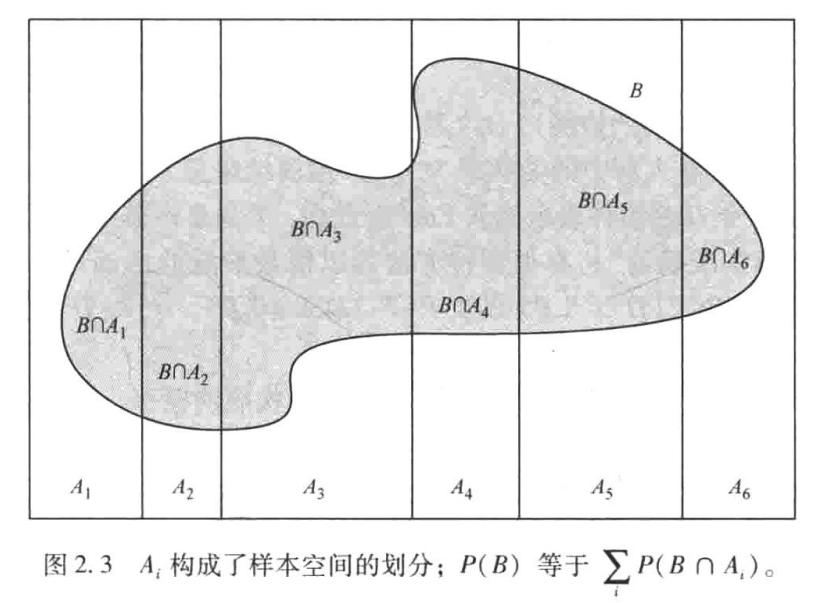
\includegraphics[width=7.5cm]{figures/全概率公式.png}
    \end{figure}

\end{frame}
\begin{frame}
  \frametitle{全概率公式( 续)}
  对于全概率公式, 我们要注意以下几点
  \begin{itemize}[<+-|alert@+>]
  \item 全概率公式的最简单形式: 如果$0<P(A)<1$, 则
    \begin{eqnarray*}
      P(B)=P(A)P(B|A)+P(\overline{A})P(B|\overline{A})
    \end{eqnarray*}
  \item 条件$A_1,A_2,\cdots,A_n$为样本空间$\Omega$的一个分割, 可改为$A_1,A_2,\cdots,A_n$互不相容, 且$B\subset \cup_{k=1}^nA_k$
  \item 在必要时,可把分割的概念推广到可列个事件($n=\infty$)的情形, 相应地有\pause
  $$ P(B)=\sum_{k=1}^{\infty} P(A_kB)=\sum_{k=1}^{\infty} P(A_k) P(B|A_k).$$
  \end{itemize}
\end{frame}



\subsection{贝叶斯公式}
\begin{frame}
	\frametitle{贝叶斯公式}
	\begin{thm}
		设$A_1,A_2,\cdots,A_n$为样本空间$\Omega$的一个分割, 即 $A_1,A_2,\cdots,A_n$互不相容, 且$\cup_{k=1}^nA_k=\Omega$, 若 $$P(B)>0, P(A_k)>0, k=1,2,\cdots,n$$ 则
		\begin{eqnarray*}
			P(A_k|B)=\dfrac{P(A_k)P(B|A_k)}{\sum_{j=1}^nP(A_j)P(B|A_j)}.
		\end{eqnarray*}
	特别的, 我们有
  \begin{eqnarray*}
    P(A|B)=\frac{P(B|A)P(A)}{P(B)}
    \end{eqnarray*}
	\end{thm}
\end{frame}


\begin{frame}{贝叶斯几率}
    \begin{defi}(\tc{几率}) 一个事件的几率(odds)为
    \begin{eqnarray*}
     ​\text{odds}(A)=P(A)/P(\overline{A})=\frac{P(A)}{1-P(A)}
     \end{eqnarray*}
    \end{defi}
  %\vspace{-0.5cm}
  \pause
  %\begin{itemize}[<+-|alert@+>]
  %\item
  \textcolor{cyan}{概率的几率表示:} $P(A)=\text{odds}(A)/(1+\text{odds(A)}) $
  %\end{itemize}
  \begin{thm} (\tc{贝叶斯公式的几率形式})对于任意两个正概率事件$A$和$B$, 给定以$B$为条件的情况下, $A$的几率如下:
   \begin{eqnarray*}
    \frac{P(A|B)}{P(\overline{A}| B)}=\frac{P(B| A)P(A)}{P(B| \overline{A})P(\overline{A})}
    \end{eqnarray*}
    \end{thm}
  \pause

  \begin{itemize}[<+-|alert@+>]
  \item 后验几率 $\dfrac{P(A|B)}{P(\overline{A}|B)}$ 等于先验几率 $\dfrac{P(A)}{P(\overline{A})}$ 乘以似然比因子 $\dfrac{P(B|A)}{P(B|\overline{A})}$. % 这个因子就是统计学中很有名的似然比.
  \item 有时候用上述形式的贝叶斯准则可以更方便地求出后验几率, 如果需要的话还可以将几率形式转换成概率形式形式.
  \end{itemize}


\end{frame}




\begin{frame}{全概率与贝叶斯内涵:由因到果,由果推因}
	\begin{itemize}[<+-|alert@+>]
		\item 在现实中把事件$B$看作结果, 把事件$A_1,A_2,\cdots, A_n$看作导致结果$B$的各种原因
		\item 全概率公式是由各种原因推理出结果事件发生的概率,是由因到果
		\item 在日常生活中常常是观察到某种现象,反推造成这种现象的各种原因的概率,即由果推因
		\item 条件概率$P(A_k|B)$, 就是在观察到结果事件$B$已经发生的情况下,推断结果事件$B$是由原因$A_k$造成的概率的大小
		\item $P(A_k)$: 先验概率, 在没有别的前提信息情况下的概率值,一般借助经验来估计,或赋予所有原因以相同的先验概率
		\item $P(A_k|B)$:后验概率, 在获得“结果事件$B$发生”这个信息之后原因$A_k$出现的概率
		\item 后验概率可看作先验概率在获取了新信息之后的一种修正, 贝叶斯公式恰恰提供了一种计算后验概率的工具

%		\item 条件概率$P(A_k|B)$通常由贝叶斯公式来计算%Bayes 公式虽然很简单, 但是它却很有哲理意义
%	%	事件原因的事前可能性估计(先验概率$P(A_k)$)$\Rightarrow$得知结果后对可能性作出新的认识(后验概率$P(A_k|B)$)
%		\item Bayes
%		\item Bayes 学派: 对概率统计问题有自己的独特理解, 但他们主张按照同等无知原则, 赋予所有原因以相同的先验概率, 常受批评
%		\item 后来有人为了取其之长避其之短, 发展出所谓经验 Bayes 方法
%		\item 在计算机广为普及的今天, Bayes 方法和经验 Bayes 方法的实用价值也随之大大提高
		\item 贝叶斯理论对于人工智能、深度学习等理论具有重要的指导意义, 贝叶斯统计受到了从未有过的青睐, 迎来了前所未有的发展机遇
	\end{itemize}
\end{frame}

\begin{frame}
  \frametitle{条件全概率公式和条件贝叶斯公式}
  \vspace{0.2cm}
    \begin{thm} (\tc{条件全概率公式}) 令$A_1,\cdots,A_n$为样本空间$\Omega$的一个划分. 设对于所有的$i$满足$P(A_iE)>0$, 则
   \begin{eqnarray*}
    P(B| E)=\sum_{i=1}^{n}P(B| A_{i},E)P(A_{i}| E)
    \end{eqnarray*}
    \end{thm}
    \pause
  \vspace{0.3cm}
  \begin{thm} (\tc{条件贝叶斯公式}) 设$P(AE)>0$且$P(BE)>0$,则有
   \begin{eqnarray*}
    P(A| B,E)=\frac{P(B| A,E)P(A| E)}{P(B| E)}
    \end{eqnarray*}
    \end{thm}

\end{frame}









\subsection{条件概率、全概率与贝叶斯公式的应用}
\begin{frame}{条件性思维谬误:控方证人的错误}
\begin{exam}\tc{(控方证人的错误)} 1988 年,Sally Clark 由于她的两个孩子在出生不久便死亡,因而被指控谋杀幼童。在审讯期间,控方的一个专家证人证实
\begin{itemize}[<+-|alert@+>]
\item 新生儿因婴儿猝死综合症 (SIDS) 而死亡的概率为 $1/8500$
\item 所以两个新生儿由于婴儿猝死综合症死亡的概率为 $(1/8500)^2$, 大约为 7300 万分之一
\item 因此,他认为 Clark 清白的概率仅为 7300 万分之一.
\end{itemize}
\end{exam}
\vspace{0.2cm}

\pause
\begin{jieda} 这个推理过程至少有两个问题
\begin{itemize}[<+-|alert@+>]
\item 一个家庭内部成员之间死于 SIDS 是否相互独立?
\begin{itemize}[<+-|alert@+>]
\item 家庭内部成员之间死于 SIDS 相互独立时,“第一个孩子死于 SIDS” 且 “第二个孩子也死于 SIDS” 的概率是相应的两个事件概率相乘
\item 如果遗传因素或其他家庭特有的风险因素导致某些家庭内的所有新生儿面临 SIDS 的风险增加,这种独立性就不再成立了.
\end{itemize}
\end{itemize}
\end{jieda}
\end{frame}

\begin{frame}{条件性思维谬误:控方证人的错误}
\begin{itemize}[<+-|alert@+>]
\item 这个所谓的专家将两个不同的条件概率混淆了: $P (\mbox{清白 | 证据})$ 和 $P (\mbox{证据 | 清白})$ 是不一样的.
\begin{itemize}[<+-|alert@+>]
\item  专家 1 声称:如果在被告人是清白的情况下,两个孩子死亡的概率很低;那就是说 $P (\mbox{证据 | 清白})$ 非常小.
\item 但人们感兴趣的是,给定现在所有的证据 (孩子均死) 条件下,报告人仍清白的概率,即 $P (\mbox{清白 | 证据})$.
\item 由贝叶斯准则可知,$$P (\mbox{清白 | 证据})=\frac{P (\mbox{证据 | 清白}) P (\mbox{清白})}{P (\mbox{证据})},$$

\item 所以为了计算 $P (\mbox{清白 | 证据})$, 这里需要考虑 $P (\mbox{清白})$, 也就是被告清白的先验概率。这个概率是很高的;
\item 虽然 SIDS 造成两个婴儿死亡是很罕见的,但是蓄意杀害两个婴儿的情况也很少见!
\item 基于现有证据的后验概率是对很低的 $P (\mbox{证据 | 清白})$ 和很高的 $P (\mbox{清白})$ 的一个平衡。专家的结果 $(1/8500)^2$ 是有问题的,它只是整个计算式中的一部分.
\end{itemize}
\end{itemize}
\end{frame}

\begin{frame}{{\rm Monty Hall}三门问题}
	\begin{exam}在 Monty Hall 主持的“Let's Make a Deal”节目中, 有三扇门, 其中有两扇门后面是一只山羊, 一扇门后面是一辆车.  选手将获得其所选中的那扇门后面的物品.
	  \begin{itemize}[<+-|alert@+>]
	  \item 一位选手从三扇最近的门中选一扇
	  \item Monty 知道车在哪扇门后面, 并以不暴露车的位置打开剩下两扇门中的一扇, 即他打开的门后面永远是山羊.
	  \item 若剩下的两扇门后都是山羊的话, Monty 会等可能地随机选一扇门.
	  \item 然后 Monty 会让对手选择, 是换另一扇没打开的门还是不换.
	  \item 如果对手的目标是得到车, 她应该换吗?
	  \end{itemize}

	  \end{exam}
	  \vspace{-0.2cm}
	   \begin{figure}[Monty Hall 问题.png]
		\centering
		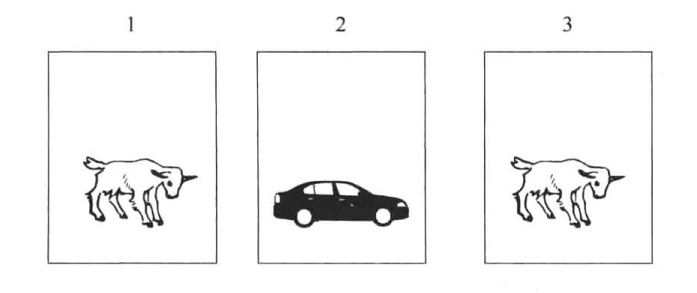
\includegraphics[width=8.5cm]{figures/Monty Hall 问题.png}
	  \end{figure}
  \end{frame}

  \begin{frame}{Monty Hall 问题(续)}
  \begin{jieda}
  \begin{itemize}[<+-|alert@+>]
  \item 先将三扇门从$1$到$3$编号. \\
  \item 不失一般性, 可以假设选手选择的是$1$号门
  \item 令
  \begin{align*}
	  A&=\{\mbox{换门得到车} \} \\
	  B&=\{\mbox{不换门得到车} \}\\
	 C_i&:=\{\mbox{车在第}i \mbox{扇门后面} \}, i=1,2,3.
  \end{align*}
  \item 显然, $P(B)=P( \mbox{不换门得到车} )=1/3$

  \item 则由全概率公式
  \begin{align*}
	  P(A)&=P(A|C_1)\cdot\frac{1}{3}+P(A|C_2)\cdot\frac{1}{3}+P(A|C_3)\cdot\frac{1}{3}\\
	 & =0\cdot\frac{1}{3}+1\cdot\frac{1}{3}+1\cdot\frac{1}{3}=\frac{2}{3}
  \end{align*}

  \end{itemize}
  \end{jieda}
  \end{frame}

  \begin{frame}{Monty Hall 三门问题图示}
	  \begin{figure}[ch1-montyhall-visual-prob.png]
		  \centering
		  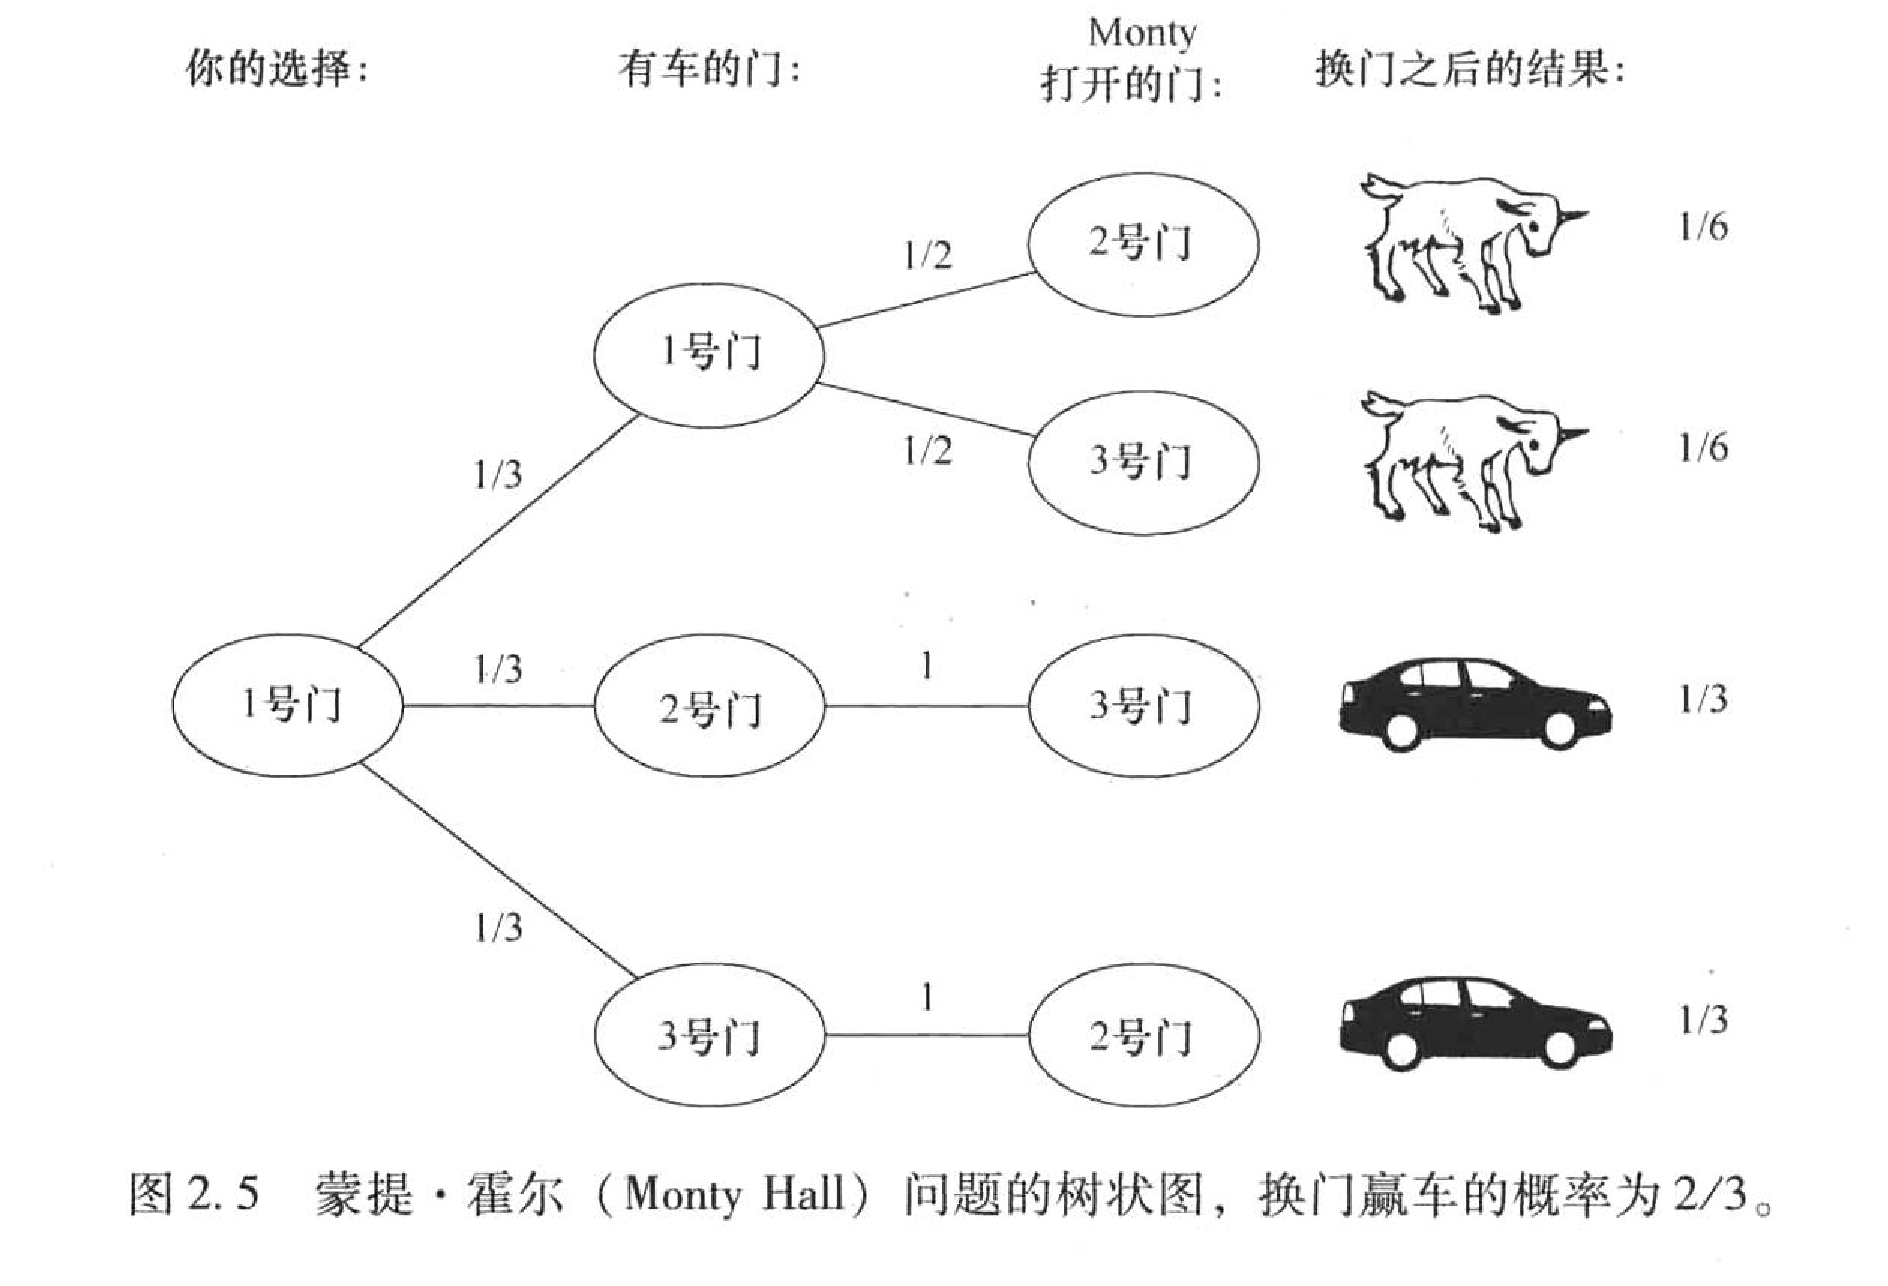
\includegraphics[width=11cm]{figures/ch1-montyhall-visual-prob.png}
		\end{figure}

  \end{frame}


  \begin{frame}{随机徘徊的吸收概率}
	\begin{exam}
		质点在数轴上整数点运动, 若质点处在整数点$i$上, 则下一时刻%
		\begin{itemize}[<+-|alert@+>]
			\item  以概率$p$向右移动到$i+1$
			\item 以概率$q$向左移动到$i-1$, 其中$p,q>0, p+q=1$
			\item 我们把质点的上述运动称之为随机徘徊或随机游动
			%\item 特殊的点$0$与$a(a>1)$
			\item 考虑数轴上的两个\textcolor{cyan}{吸收壁$0$与$a(a>1)$}:质点运动到$0$或$a$之后就永远不再移动
			\item 现求自$i(0<i<a)$出发的质点将被$0$或$a$吸收的概率
		\end{itemize}
	\end{exam}
\end{frame}


\begin{frame}
	\vspace{0.5cm}
	\hspace{-0.2cm}\jieda 令 $E_i=\{\mbox{质点自}i\mbox{出发}\}, F=\{\mbox{质点在}0\mbox{被吸收}\}, G=\{\mbox{质点在}a\mbox{被吸收}\}$. \pause

	下面对$i=0,1,\cdots,a$ 计算
	\begin{eqnarray*}
		P_i=P(F|E_i), \quad Q_i=P(G|E_i)
	\end{eqnarray*}
	\pause 记$B=\{\mbox{质点第一次向左移动 1 单位}\}$并以第 1 次可能的运动情
	况为条件进行全概率展开可得
	\begin{eqnarray*}
		Q_i&=&P(GB|E_i)+P(G\bar{B}|E_i)\\
		&=&P(B|E_i)P(G|BE_i)+P(\bar{B}|E_i)P(G|\bar{B}E_i)\\
		&=&pQ_{i+1}+qQ_{i-1}, \quad i=1,2,\cdots a-1.
	\end{eqnarray*}
	\pause 将上述递推式重写为
	\begin{eqnarray}\label{eq:ditui1}
		Q_{i+1}-Q_i=\dfrac{q}{p}(Q_i-Q_{i-1}), \quad i=1,\cdots, a-1.
	\end{eqnarray}

\end{frame}

\begin{frame}
	\vspace{0.5cm}
	\begin{enumerate}[<+-|alert@+>]
		\item 当$p=q=1/2$时, 由$Q_0=0$及$Q_a=1$可得
		\begin{eqnarray*}
			Q_i=\dfrac{i}{a},\quad  i=0,\cdots, a.
		\end{eqnarray*}
		\item 当$p\neq q$时, 反复利用递推式\eqref{eq:ditui1}并注意到$Q_0=0$可导出
		\begin{eqnarray}\label{eq:ditui2}
			Q_{i+1}-Q_i=\bigg(\dfrac{q}{p}\bigg)^iQ_1, \quad i=1,\cdots, a-1.
		\end{eqnarray}
		\pause 上式对$i=1,\cdots, a-1$求和并利用$Q_a=1$可得
		\begin{eqnarray*}
			Q_1=\bigg[\sum_{i=0}^{a-1}\bigg(\dfrac{q}{p}\bigg)^{i}\bigg]^{-1}=\dfrac{1-q/p}{1-(q/p)^a}
		\end{eqnarray*}
		\pause 再将(\ref{eq:ditui2})式对$i=1,\cdots, i-1$求和并将上述$Q_1$代入可得
		\begin{eqnarray*}
			Q_i=\dfrac{1-(q/p)^i}{1-(q/p)^a}, \quad i=0,\cdots, a.
		\end{eqnarray*}

	\end{enumerate}
\end{frame}

\begin{frame}
	综上可得
	\begin{eqnarray*}
		Q_i=\left\{
		\begin{array}{cl}
			\dfrac{i}{a}, &p=q,\\
			\\
			\dfrac{1-(q/p)^i}{1-(q/p)^a}, &p\neq q.
		\end{array}
		\right.
	\end{eqnarray*}
	类似可得



	\begin{eqnarray*}
		P_i=\left\{
		\begin{array}{cl}
			\dfrac{a-i}{a}, &p=q,\\
			\\
			\dfrac{(q/p)^i-(q/p)^a}{1-(q/p)^a}, &p\neq q.
		\end{array}
		\right.
	\end{eqnarray*}


\end{frame}



\begin{frame}{Simpson 悖论}
	\begin{exam}
		有两种治疗肾结石的方案,其治疗效果如下:
		\begin{itemize}[<+-|alert@+>]
			\item \textcolor{cyan}{方案$1$:} 小结石患者占$25\%$, 大结石患者占$75\%$, 小结石患者的治愈率是$93\%$, 大结石患者的治愈率是$73\%$
			\item \textcolor{cyan}{方案$2$:} 小结石患者占$77\%$, 大结石患者占$23\%$, 小结石患者的治愈率是$87\%$, 大结石患者的治愈率是$69\%$
			\item 不管是对小结石患者, 还是大结石患者, 方案$1$的治愈率都要高于方案$2$
			\item \textcolor{red}{方案$1$优于方案$2$吗?}
		\end{itemize}
	\end{exam}
	\pause
	\begin{jieda}
		计算两种方案的治愈率
		\begin{itemize}[<+-|alert@+>]
			\item 记$A$=\{患者是小结石患者\}, $B$=\{患者被治愈\}
			\item 根据全概率公式\pause
			\begin{align*}
				&\hspace{-0.5cm}P_1(B)=\pause P_1(A)P_1(B|A)+P_1(\overline{A})P_1(B|\overline{A})=\pause 0.25·0.93+0.75·0.73=0.78\pause \\
				&\hspace{-0.5cm} P_2(B)=\pause P_2(A)P_2(B|A)+P_2(\overline{A})P_2(B|\overline{A})=\pause 0.77·0.87+0.23·0.69=0.8286
			\end{align*}
			\item 方案$2$的治愈率高于方案$1$, 可见方案$1$并不优于方案$2$
		\end{itemize}
	\end{jieda}
\end{frame}

\begin{frame}
	\frametitle{敏感性问题调查}
	敏感性问题调查方案的关键在于要使被调查者愿意作出真实的回答又能保守个人秘密, 如果调查方案有误, 被调查者就会拒绝配合, 所得调查数据将失去真实性.
	\pause
	\vspace{0.5cm}

	{\bf 调查方案: } 被调查者只需要加答以下两个问题中的一个问题,且只需要回答“是”或“否”.

	\pause
	问题 A: 你的生日是否在 7 月 1 日之前?

	问题 B: 所调查的敏感性问题.

	\pause
	\vspace{0.5cm}
	{\bf 调查方案的操作: }

	( 1)被调查者在没有旁人的情况下独自一人在房间内操作回答问题

	\pause
	( 2)被调查者从一个罐子中随机抽一球, 看过颜色后放回, 若抽到白球, 回答问题 A, 抽到红球, 回答问题 B.

	( 3)被调查者无论回答问题 A 还是问题 B, 只需在仅有“是”与“否”选项的答卷上作答然后将答卷放入密封的投票箱内.

\end{frame}

\begin{frame}
	\frametitle{敏感性问题调查}
	{\bf \textcolor{red}{问题:}} 假若我们有$n$张问卷, 其中$k$张回答“是”, 我们如何确定选定红球回答问题 B 为“是”的概率?


	\pause
	{\bf \textcolor{red}{已知:}}
	\begin{itemize}[<+-|alert@+>]
		\item 红白球的比例, 即$P(\mbox{红球}):=\pi, P(\mbox{白球})=1-\pi$;
		\item $P(\mbox{是}|\mbox{白球})=0.5$;
		\item $P(\mbox{是})\approx \dfrac{k}{n}$.
	\end{itemize}
	\pause
	{\bf \textcolor{red}{待求:}} $p:=P(\mbox{是}|\mbox{红球})$.

	\pause
	{\bf\jieda} 由全概率公式可得
	\begin{eqnarray*}
		P(\mbox{是})=P(\mbox{白球})P(\mbox{是}|\mbox{白球})+P(\mbox{红球})P(\mbox{是}|\mbox{红球})
	\end{eqnarray*}
	即\pause
	\begin{eqnarray*}
		\dfrac{k}{n}\approx (1-\pi)\cdot 0.5+\pi\cdot p \Rightarrow p=\dfrac{k/n-0.5(1-\pi)}{\pi}
	\end{eqnarray*}


\end{frame}

\begin{frame}{{\rm Bayesian}滤波}
\begin{itemize}[<+-|alert@+>]
	\item 许多工程科学类问题都可以归结为如下图所示形式
	\begin{figure}[htbp]\nonumber
		\centering
		\includegraphics<+->[width=9.19cm, height=3cm]{BayesianFilter.jpg}
		% \caption{}
  %\onslide<4->\centering{\small 心灵捕手 }
	  \end{figure}
	\item  系统自身的状态 \( X \) 是我们关注的随机事件,但是由于技术手段等方面的限制,无法直接对 \( X \) 进行观测, 只能获取另一随机事件, 即间接反映系统状态 \( X \) 的观测量 \( Z \).
	\item 问题转化为已知观测量 \( Z \) 的条件下, 如何对系统状态 \( X \) 进行推断.用条件概率的语言讲, 就是计算 \( P(X \mid Z) \).
	\item 通常情况下, \( X \) 和 \( Z \) 随时间变化,分别记作 \( X_{n} \) 和 \( Z_{n} \) ,其中 \( n \) 表示时间. 那么在实际应用中, 到 \( n \) 时刻为止, 我们掌握的实际观测数据为 \( \left\{Z_{1}, \cdots, Z_{n}\right\} \),
\end{itemize}


\end{frame}


\begin{frame}{{\rm Bayesian}滤波}
\begin{itemize}[<+-|alert@+>]
	\item 如何实现 $P\left(X_{n} | Z_{1}, \cdots, Z_{n}\right) \longrightarrow P\left(X_{n+1} | Z_{1}, \cdots, Z_{n+1}\right)$的递推计算?
	\item 注意到, 若已知$X_{n+1}$时,$Z_{n+1}$与$\left\{Z_{1}, \cdots, Z_{n}\right\}$独立, 则\pause
	{\small\begin{eqnarray*}
		P\left(X_{n+1} | Z_{1}, \cdots, Z_{n+1}\right)\pause&=& \frac{P\left(X_{n+1}, Z_{1}, \cdots, Z_{n+1}\right)}{P\left(Z_{1}, \cdots, Z_{n+1}\right)}\\
		\pause&=&\frac{P\left(Z_{n+1} | X_{n+1}, Z_{1}, \cdots, Z_{n}\right) P\left(X_{n+1}, Z_{1}, \cdots, Z_{n}\right)}{P\left(Z_{1}, \cdots, Z_{n+1}\right)}\\
		\pause&=&\frac{P\left(Z_{n+1} | X_{n+1}\right) P\left(X_{n+1}, Z_{1}, \cdots, Z_{n}\right)}{P(Z_{n+1}|Z_{1}, \cdots, Z_n)P\left(Z_{1}, \cdots, Z_{n+1}\right)}\pause
	\end{eqnarray*}}




\end{itemize}



\end{frame}

\begin{frame}{{\rm Bayesian}滤波}
	\begin{itemize}[<+-|alert@+>]
		\item 再由\pause
		{\small \begin{eqnarray*}
			&&P\left(X_{n+1}, Z_{1}, \cdots, Z_{n}\right)\\
			&=&\pause\sum_{X_{n}} P\left(X_{n+1}, X_{n}, Z_{1}, \cdots, Z_{n}\right) \\
			&=&\pause\sum_{X_{n}} P\left(X_{n+1} | X_{n}, Z_{1}, \cdots, Z_{n}\right) P\left(X_{n} | Z_{1}, \cdots, Z_{n}\right) P\left(Z_{1}, \cdots, Z_{n}\right) \\
			&=&\pause\sum_{X_{n}} P\left(X_{n+1} | X_{n}\right) P\left(X_{n} | Z_{1}, \cdots, Z_{n}\right) P\left(Z_{1}, \cdots, Z_{n}\right)\pause
		\end{eqnarray*}}
	    \item 将上式代入前面一页表达式中可得
	{\small \[
		\hspace{-0.3cm} P\left(X_{n+1} | Z_{1}, \cdots, Z_{n+1}\right)\pause=\frac{P\left(Z_{n+1} | X_{n+1}\right)}{P\left(Z_{n+1} | Z_{n}, \cdots, Z_{1}\right)} \sum_{X_{n}} P\left(X_{n+1} | X_{n}\right) P\left(X_{n} | Z_{1}, \cdots, Z_{n}\right)\]}
		\item 上式便是对系统状态进行递推估计的 Bayesian 滤波公式,在雷达、声呐、通信、导航、机器学习等许多领域有广泛应用.

	\end{itemize}






	\end{frame}
%%% Local Variables:
%%% mode: latex
%%% TeX-master: t
%%% End:

 

\title[概率论]{第八讲: 事件的独立性}
%\author[张鑫 {\rm Email: xzhangseu@seu.edu.cn} ]{\large 张 鑫}
\institute[东南大学数学学院]{\large \textrm{Email: xzhangseu@seu.edu.cn} \\ \quad  \\
	\large 东南大学\quad 数学学院\\
	\vspace{0.3cm}
	%\trc{ 公共邮箱: \textrm{zy.prob@qq.com}\\
		% \hspace{-1.7cm}  密\qquad 码: \textrm{seu!prob}}
}
\date{}

{\setbeamertemplate{footline}{}
	\begin{frame}
		\titlepage
	\end{frame}
}
\subsection{事件的独立性}

\begin{frame}
  \frametitle{两个事件的独立性}
  \begin{itemize}[<+-|alert@+>]
  \item 直观上来说,两个事件的独立性是指:一个事件的发生不影响另一个事件的发生。比如在掷两颗骰子的实验中,第一颗骰子的点数和第二颗骰子的点数是互不影响的.
  \item 从概率的角度看,$P (A|B)$ 与 $P (A)$ 的差别在于:事件 $B$ 的发生改变了事件 $A$ 发生的概率,也即事件 $B$ 对事件 $A$ 有某种影响。故如果 $A$ 与 $B$ 的发生是相互不影响的,则有 \pause
    \begin{eqnarray*}
      P(A|B)=P(A),\quad P(B|A)=P(B).
    \end{eqnarray*}
    \pause 上面两式均等价于
    \begin{eqnarray}\label{eq:inden}
      P(AB)=P(A)P(B)
    \end{eqnarray}
  \item 注意到 \eqref{eq:inden} 式对 $P (B)=0$ 或 $P (A)=0$ 仍然成立,为此,我们用 \eqref{eq:inden} 作为两个事件相互独立的定义.
  \end{itemize}
\end{frame}

\begin{frame}
  \frametitle{两个事件独立性的定义}
  \begin{defi}
    如果对事件 $A$ 与 $B$ 有
    \begin{eqnarray*}
      P(AB)=P(A)P(B)
    \end{eqnarray*}
    成立,则称 \textcolor{red}{事件 $A$ 与 $B$ 相互独立}, 简称 \textcolor{red}{$A$ 与 $B$ 独立}. 否则称 $A$ 与 $B$ 不独立或相依.
  \end{defi}

\begin{rmk}
	\begin{itemize}
		\item 零概率事件 $E$ 与任何事件相互独立,特别的,不可能事件与任何事件相互独立
		\item 若$A, B$互不相容且独立, 则$A, B$至少有一个零概率事件
        \item 非零概率不相容事件,一定不独立; 非零概率独立事件,一定相容
        \item 若事件$A$与其自身相互独立,则$P(A)=0$, 或$P(A)=1$
\end{itemize}


\end{rmk}

\pause
  \textcolor{red}{如何确定事件的独立性: }
  \begin{itemize}[<+-|alert@+>]
  \item 实际问题中,两个事件的独立大多根据经验及相互有无影响的直观性来判断.
  \item 但对于较复杂事件,有无相互影响并不是很直观,则需要验证 \eqref{eq:inden} 式是否成立来说明独立性.
  \end{itemize}
\end{frame}


 \begin{frame}
	\frametitle{对立事件的独立性}
	\begin{thm}
		若 $A$ 与 $B$ 独立,则 $A$ 与 $\overline{B}$ 独立,$\overline{A}$ 与 $B$ 独立,$\overline{A}$ 与 $\overline{B}$ 独立.
	\end{thm}
	\pause

	\zheng 我们仅证 $P (A\overline{B})=P (A) P (\overline{B})$, 其余类似可证.
	\begin{eqnarray*}
		P(A\overline{B})&=&\pause P(A-B)=\pause P(A)-P(AB)\pause =P(A)-P(A)P(B)\\
		&=&\pause P(A)(1-P(B))=\pause P(A)P(\overline{B})
	\end{eqnarray*}

	\pause
	对于上面的定理直观上来理解也是很容易的:因 $A,B$ 独立,故 $A$ 的发生不影响 $B$ 的发生,从而也不会影响 $B$ 的不发生,$\cdots$
\end{frame}


\begin{frame}{概率测度与独立性的关系}
  \begin{exam}
    考虑掷硬币问题, 记正面向上对应的样本点为 "$H$", 反面向上为 "$T$", 那么连续掷三次的结果构成样本空间
  \[
  \Omega=\{H H H, H H T, H T H, H T T, T H H, T H T, T T H, T T T\},
  \]
    令事件$A$为 "最后一次是反面", $B$为 "三次结果相同", 则有
  \[
  A=\{H H T, H T T, T H T, T T T\},  B=\{H H H, T T T\}
  \]试讨论 $A, B$的独立性.
  \end{exam}
\pause

\jieda: 设每次抛掷反面向上的概率是$p$, 那么\pause
\[
P(A)=p^{3}+2 p^{2}(1-p)+p(1-p)^{2}, \pause  P(B)=p^{3}+(1-p)^{3},  P(A B)=p^{3},
\]
\pause
不难验证, $p=0$、$p=1$和$p=\frac{1}{2}$时,$A$和$B$是独立的, 否则两者不独立.


\end{frame}







   \begin{frame}
	\frametitle{三个事件的独立性}
	\begin{defi}
		设 $A,B,C$ 三个事件,如果有
		\begin{eqnarray}\label{eq:inden1}
			\left.\begin{array}{l}
				P(AB)=P(A)P(B)\\
				P(AC)=P(A)P(C) \\
				P(BC)=P(B)P(C)
			\end{array}\right\}\\
			\label{eq:inden2}
			P(ABC)=P(A)P(B)P(C)
		\end{eqnarray}
		则称 $A,B,C$ 相互独立。如果仅有 \eqref{eq:inden1} 式成立,则称 $A,B,C$ 两两独立.
	\end{defi}
\end{frame}

\begin{frame}
	\frametitle{两两独立与相互独立的关系}
	\begin{itemize}[<+-|alert@+>]
		\item 由定义可知,三个事件相互独立必能推出两两独立.
		\item 但两两独立未必能推出相互独立,即 \eqref{eq:inden1} 式成立,不一定能推出 \eqref{eq:inden2} 成立
		\begin{itemize}
			\item 考虑独立投掷两枚均匀硬币的随机试验,设事件 $A$ 代表第一枚硬币正面朝上,事件 $B$ 代表第二枚硬币正面朝上,事件 $C$ 表示两枚硬币结果相同。易知: \pause
			$A$ $B$ 和 $C$ 是两两独立,但
			\begin{align*}
				P(A\cap B\cap C)=1/4\neq 1/8=P(A)P(B)P(C).
			\end{align*}
			\item 考虑一个均匀的正四面体,第一二三面分别染上红 / 白 / 黑色,第四面同时染上红白黑色。现在以 $A,B,C$ 分别记投一次四面体出现红,白,黑色朝下的事件。则易有 \pause
			\begin{eqnarray*}
				P(A)=P(B)=P(C)=\pause 1/2\\ \pause
				P(AB)=P(BC)=P(AC)=\pause 1/4\\ \pause
				P(ABC)=\pause 1/4    \pause
			\end{eqnarray*}
		\end{itemize}\vspace{-0.7cm}
	\end{itemize}
\end{frame}

		\begin{frame}
			\frametitle{两两独立与相互独立的关系}
			\begin{itemize}[<+-|alert@+>]
		\item 反之,如果 \eqref{eq:inden2} 成立,是否能推出 \eqref{eq:inden1} 成立?
		\begin{itemize}[<+-|alert@+>]
			\item 考虑一个均匀的正八面体,第 1, 2, 3, 4 面染上红色,第 1, 2, 3, 5 面染上白色,第 1, 6, 7, 8 面染上黑色。现在以 $A,B,C$ 分别记投一次八面体出现红,白,黑色朝下的事件,则 \pause
			\begin{eqnarray*}
				P(A)=P(B)=P(C)=\pause 4/8=1/2\\ \pause
				P(ABC)=\pause 1/8   \\ \pause
				P(AB)=3/8\pause \neq 1/4=P(A)P(B)
			\end{eqnarray*}
		\end{itemize}
	\end{itemize}
\end{frame}

\begin{frame}
	\frametitle{三个以上事件的独立性}
	\begin{defi}
		设 $(\Omega,\mathcal{F}, P)$ 为一概率空间,$A_1,A_2,\cdots,A_n\in\mathcal{F}$, 对任意的 $1\le k\le n$ 及任意的 $1< j_1<j_2<\cdots<j_k\leq n$ 均有:
		\begin{eqnarray}\label{eq:mulinden0}
			P(A_{j_1}A_{j_2}\cdots A_{j_k})=P(A_{j_1})P(A_{j_2})\cdots P(A_{j_k})
		\end{eqnarray}
		成立,则称事件 $A_1,\cdots, A_n$ 相互独立.
	\end{defi}
	\pause
	\begin{itemize}[<+-|alert@+>]
		\item \eqref{eq:mulinden0} 式共有多少个等式?\pause
		\begin{eqnarray}
			\label{eq:mulinden}
			\left.\begin{array}{l}
				P(A_{j_1}A_{j_2})=P(A_{j_1})P(A_{j_2})\\
				P(A_{j_1}A_{j_2}A_{j_3})=P(A_{j_1})P(A_{j_2})P(A_{j_3}) \\
				\qquad \vdots\\
				P(A_1A_2\cdots A_n)=P(A_1)P(A_2)\cdots P(A_n)
			\end{array}\right\} \pause \textcolor{red}{C_n^2+\cdots+C_n^n=2^n-n-1}
		\end{eqnarray}
		\pause
		\item 从定义可以看出,$n$ 个相互独立事件中的任取 $m$($2\le m\le n$) 个事件仍是相互独立的,而且任意一部分与另一部分也是独立的.
		\item 类似于前面的证明,将相互独立事件中的任一部分换为对立事件,所得诸事件仍是相互独立的.
	\end{itemize}



\end{frame}

\begin{frame}
	\frametitle{任意多个事件相互独立}
	\begin{defi}
		设 $(\Omega,\mathcal{F}, P)$ 为一概率空间,每个 $t\in T$ 有 $A_t\in \mathcal{F}$. 称 $\{A_t, t\in T\}$ 为独立事件族,如果对 $T$ 的任意有限子集 $\{t_1,t_2,\cdots, t_s\}$, 事件 $A_{t_1}, A_{t_2},$ $\cdots, A_{t_s}$ 相互独立.
	\end{defi}


	\vspace{0.8cm}
	\pause
	\begin{exam}
		$\mathcal{F}$ 中事件序列 $\{A_n\}$ 为相互独立的充分必要条件是,任意 $n\geq 1$, 事件 $A_1,A_2, \cdots, A_n$ 独立;等价的,任意有限个自然数 $k_1,\cdots, k_s$ 有
		\begin{eqnarray*}
			P(A_{k_1}A_{k_2}\cdots A_{k_s})=P(A_{k_1})P(A_{k_2})\cdots P(A_{k_s})
		\end{eqnarray*}

	\end{exam}

\end{frame}


\begin{frame}{条件独立}
\begin{defi}
称事件 $A$ 和 $B$ 是关于 $E$ 条件独立的,如果 $$P (A\cap B|E)=P (A|E) P (B|E)$$
\end{defi}
\pause
\begin{itemize}[<+-|alert@+>]
\item 两个事件可以在给定事件 $E$ 的条件下是条件独立的,但它们不是独立的.
\item 两个事件可以是独立但却不是关于 $E$ 条件独立的.
\item 两个事件可以关于 $E$ 条件独立但关于 $\overline{E}$ 不存在条件独立.
\end{itemize}
\end{frame}

\begin{frame}{条件独立不意味着独立}
\begin{exam}
假设有两枚硬币,一枚是均匀的,一枚是不均匀的。从两枚硬币中随机的选一枚硬币并进行抛掷 2 次,若令
\begin{align*}
  F &:=\{\mbox{选取的硬币是均匀的}\}\\
   A_{1}&:= \{\mbox{第一次投掷硬币正面朝上}\}\\
   A_{2}&:= \{\mbox{第二次投掷硬币正面朝上}\}
\end{align*}
则给定 $F$ 为条件,$A_1$ 和 $A_2$, 是相互独立的,$A_1$ 和 $A_2$ 并不是无条件独立的,因为 $A_1$ 会提供关于 $A_2$ 的信息.
\end{exam}
\end{frame}

\begin{frame}{独立不意味着条件独立}
\begin{exam}
假设只有我的朋友 Alice 和 Bob 给我打过电话。每天他俩都会相互独立地决定是否给我打电话。若令
\begin{align*}
	 A&:= \{\mbox{Alice 给我打电话}\}\\
	 B&:= \{\mbox{Bob 给我打电话}\}\\
     R&:=\{\mbox{听到电话铃响}\}
  \end{align*}
  \pause
  \begin{itemize}[<+-|alert@+>]
  \item 显然,$A$ 和 $B$ 是无条件独立的.
  \item 但现在我听到一声电话铃响,那 $A$ 和 $B$ 就不再独立了:如果这个电话不是 Alice 打的,那就肯定是 Bob 打的。从而 \pause
  $$P(B|R)<1=P(B|\overline{A}R)= \frac{P(B\overline{A}R)}{P(\overline{A}R)}= \frac{P(B\overline{A}|R)}{P(\overline{A}|R)}.$$
  显然: $P (B\overline{A}|R)>P (B|R) P (\overline{A}|R)$
  \item $B$ 与 $\overline{A}$ 关于 $R$ 不条件独立,$A,B$ 亦是如此.
  \end{itemize}

\end{exam}
\end{frame}

\begin{frame}{给定 $E$ 条件独立 $vs$ 给定 $\overline{E}$ 条件独立}
\begin{exam}
\label{27}
假设有两种课程:好的课程和坏的课程。在好的课上,如果你努力,就很有可能得到 $A$. 在坏的课上,教授随机分配给学生分数,而不管他们是否努力。若令
\begin{align*}
	G&:= \{\mbox{这个课程是好的}\}\\
	W&:= \{\mbox{你学习努力}\}\\
	A&:=\{\mbox{你的得分为} A\}
 \end{align*}
 \pause 这时,给定 $\overline{G}$, $A$ 和 $W$ 是条件独立的,但给定 $G$, $A$ 和 $W$ 却不是独立的!

\end{exam}
\end{frame}

\begin{frame}{集类(族)的独立性}
\begin{defi}
  \tc{(集类(族)的独立性)} 考虑样本空间$\Omega, \mathcal{A}_{k} \subset \Omega$, $k=1,\cdots, n$. 称集类(族)$\left\{\mathcal{A}_{k}\right\}_{k=1}^{n}$是相互独立的, 如果$\left\{\mathcal{A}_{k}\right\}_{k=1}^{n}$满足
\[
P\left(\bigcap_{k \in I} A_{k}\right)=\prod_{k \in I} P\left(A_{k}\right),  \forall A_{k} \in \mathcal{A}_{k},  \forall I \subset\{1,2, \cdots, n\}.
\]
\end{defi}
\pause

\begin{thm}
  \tc{(\(\sigma\)-代数的独立性)} 设 \( \mathcal{F}_{1}, \cdots, \mathcal{F}_{n} \) 为\( \Omega \)上的 \( \sigma\)-代数, 若
\[
P\left(A_{1} A_{2} \cdots A_{n}\right)=P\left(A_{1}\right) P\left(A_{2}\right) \cdots P\left(A_{n}\right), \quad \forall A_{k} \in \mathcal{F}_{k}, k=1,2, \cdots, n
\]

则 \( \mathcal{F}_{1}, \mathcal{F}_{2}, \cdots, \mathcal{F}_{n} \) 是独立的.
\end{thm}

\pause

\begin{exam}
  \tc{(硬币实验的独立性)} 抛掷不均匀硬币的实验,正面(用 1 表示)向上的概率是 \( p \), 反面 (用 0 表示) 向上的概率是 \( q \). 假设连抛 \( n \) 次, 则样本空间 \( \Omega \) 为$\Omega=\left\{a_{1} a_{2} \cdots a_{n}: a_{k}=0,1\right\}$. \pause 考虑事件$A_{k}=\left\{a_{k}=1\right\}$, $k=1,\cdots, n$, 构造 \( \sigma\)-代数 \( \mathcal{F}_{k} \): \pause $\mathcal{F}_{k}=\left\{\Omega, \varnothing, A_{k}, A_{k}^{C}\right\}$.\pause  可以验证, 这些 \( \sigma\)-代数是独立的.
\end{exam}


\end{frame}

\begin{frame}{独立的集类(族)生成的$\sigma$-代数未必独立}


\begin{itemize}[<+-|alert@+>]
  \item 考虑$\Omega=\{1,2,3,4\}$, 集类(族)$\mathcal{A}=\{\{1,2\},\{2,3\}\}$,$ \mathcal{B}=\{\{2,4\}\}$
  \item 令$P(\{1\})=P(\{2\})=P(\{3\})=P(\{4\})=\dfrac{1}{4}$, 则
  \[P(\{1,2\} \cap\{2,4\})=P(\{2\})=\frac{1}{4}=\frac{1}{2} \times \frac{1}{2}=P(\{1,2\}) P(\{2,4\}), \]
  \[P(\{2,3\} \cap\{2,4\})=P(\{2\})=\frac{1}{4}=\frac{1}{2} \times \frac{1}{2}=P(\{2,3\}) P(\{2,4\})\]
  \item 集类(族)$\mathcal{A}$和$\mathcal{B}$独立
  \item 但由于
  \[
  \sigma(\mathcal{A})=2^{\Omega},  \sigma(\mathcal{B})=\{\{2,4\},\{1,3\}, \varnothing, \Omega\}
  \]
  且明显有
  \[
  P(\{2,4\} \cap\{3\})=0 \neq \frac{1}{8}=\frac{1}{2} \times \frac{1}{4}=P(\{2,4\}) P(\{3\})
  \]
  \item 故, $\sigma(\mathcal{A})$和$\sigma(\mathcal{B})$不独立.
\end{itemize}




\end{frame}

\begin{frame}{独立的$\pi$-类(族)生成$\sigma$-代数独立}
\begin{thm}
如果$\mathcal{A}$和$\mathcal{B}$是独立的集类(族), $\mathcal{B}$是$\pi$-类, 那么$\mathcal{A}$和$\sigma(\mathcal{B})$也独立.
\end{thm}
\pause

\zheng 应用单调类定理.
\begin{itemize}[<+-|alert@+>]
  \item 任意固定$A \in \mathcal{A}$, 令
\[
\mathscr{A}=\{B \in \sigma(\mathcal{B}): P(A B)=P(A) P(B)\}
\]
则$\mathscr{A}$是$\lambda$-类(系统)

\item 由$\mathcal{B} \subset \mathscr{A}$及单调类定理可得: $\sigma(\mathcal{B}) \subset \mathscr{A}$.
\item $\mathcal{A}$和$\sigma(\mathcal{B})$独立.


\end{itemize}


\end{frame}


\begin{frame}
  \frametitle{Borel-Cantelli引理}
  \begin{thm}
    对于事件列$\{A_j\}$,有
    \begin{itemize}[<+-|alert@+>]
    \item 如果$\sum_{j=1}^\infty P(A_j)<\infty$,则$P(A_n\ i.o.)=0$
    \item 如果$\{A_j\}$相互独立,$\sum_{j=1}^\infty P(A_j)=\infty$,则$P(A_n\ i.o.)=1$
    \end{itemize}
  \end{thm}\pause
  \zheng 注意到
  \begin{eqnarray*}
    P(A_n\ i.o.)=\pause P(\lim_{n\rightarrow\infty} \cup_{j=n}^\infty A_j)=\pause \lim_{n\rightarrow\infty} P(\cup_{j=n}^\infty A_j)\le \pause \lim_{n\rightarrow\infty}\sum_{j=n}^\infty P(A_j)\pause =0
  \end{eqnarray*}
  \pause
  由于\pause
  \begin{eqnarray*}
    P(\cup_{j=n}^\infty A_j)&=&\pause \lim_{m\rightarrow\infty}P(\cup_{j=n}^m A_j)=\pause \lim_{m\rightarrow\infty}(1-P(\cap_{j=n}^m\overline{A}_j))\\\pause
    P(\cap_{j=n}^m\overline{A}_j)&=&\pause \Pi_{j=n}^m P(\overline{A}_j)=\Pi_{j=n}^m(1-P(A_j))\\
                            &\le&\pause \Pi_{j=n}^m \exp(-P(A_j))=\exp(-\sum_{j=n}^m P(A_j))\pause \stackrel{m\rightarrow\infty}{\longrightarrow} 0
  \end{eqnarray*}

\end{frame}






\subsection{随机试验的独立性}
 \begin{frame}{随机试验的独立性}

  \begin{itemize}[<+-|alert@+>]
  \item 先考虑两个随机试验,假定 $(\Omega_i,\mathcal{F}_i,P_i), i=1,2$ 为第 $i$ 个随机试验对应的概率空间。按照之前独立性的理解,两个试验的独立性应当叙述为:\pause
   \textcolor{red}{ \begin{eqnarray*}
      &&\mbox{对任何的} A_i\in\mathcal{F}_i, i=1,2, A_1\mbox{与} A_2\mbox{同时}\\
      &&\mbox{发生的概率等于它们各自概率之乘积}
    \end{eqnarray*}}%
\item 两个不妥:
  \begin{itemize}[<+-|alert@+>]
  \item ``$A_1$ 与 $A_2$ 同时发生" 应当是这两个事件的交,但它们分别是两个样本空间 $\Omega_1,\Omega_2$ 的子集,无法进行运算;
  \item 两个概率空间有各自的概率 $P_1, P_2$, 但涉及两个度验,命题中 ``同时发生的概率" 既不能用 $P_1$ 也不能用 $P_2$ 来度量.
  \end{itemize}
\item 解决方法:构造可以同时描述两个试验的新概率空间 $(\Omega,\mathcal{F},P)$.
  \end{itemize}
\end{frame}
\begin{frame}
  \frametitle{乘积空间的构造}
  \begin{itemize}[<+-|alert@+>]
  \item 样本乘积空间: $\Omega:=\Omega_1\times \Omega_2=\{(\omega_1,\omega_2):\omega_1\in\Omega_1\mbox{且}\omega_2\in \Omega_2\}$;
  \item 乘积 $\sigma$- 代数 $\mathcal{F}_1\times\mathcal{F}_2$:
    \begin{itemize}[<+-|alert@+>]
    \item 可测矩形集类: $\mathcal{G}:=\{A_1\times A_2: A_1\in\mathcal{F}_1, A_2\in \mathcal{F}_2\}$;
    \item $\mathcal{F}_1\times \mathcal{F}_2:=\sigma(\mathcal{G})$
    \end{itemize}
  \item 乘积概率测度:
    \begin{itemize}[<+-|alert@+>]
    \item 对于每个可测矩形 $A_1\times A_2\in \mathcal{G}$ 定义如下集函数:
      \begin{eqnarray}\label{eq:timeprob}
        P(A_1\times A_2)=P_1(A_1)P_2(A_2), \quad A_i\in\mathcal{F}_i, i=1,2.
      \end{eqnarray}
    \item 理论上可以证明如上定义在 $\mathcal{G}$ 上的集函数 $P$ 可唯一地扩张为 $\mathcal{F}_1\times\mathcal{F}_2$ 上的概率测度,称之为 $P_1$ 与 $P_2$ 的乘积 (概率) 测度.
    \end{itemize}
  \item 在上述乘积测度下
    \begin{eqnarray*}
      &&P(A_1\times \Omega_2)=P_1(A_1), \quad P(\Omega_1\times A_2)=P_2(A_2)\\\pause
      &&\pause P\big((A_1\times \Omega_2)\cap (\Omega_1\times A_2)\big)=\pause P(A_1\times A_2)\\
      &&\pause = P_1(A_1)P_2(A_2)=\pause P(A_1\times\Omega_1)P(\Omega_1\times A_2)
    \end{eqnarray*}
  \item $(\Omega_i,\mathcal{F}_i,P_i)$ 的独立性取决于乘积样本空间 $\Omega_1\times\Omega_2$ 上的概率是否取作由 (\ref{eq:timeprob}) 所确定的乘积测度
  \end{itemize}
\end{frame}
\begin{frame}
  \frametitle{$n$ 个试验相互独立的定义}
  \begin{defi}
    设有 $n$ 个随机试验,第 $i$ 个试验的概率空间为 $(\Omega_i,\mathcal{F}_i,P_i),$ $ i=1,\cdots,n$. 代表这 $n$ 个试验的乘积样本空间 $\Omega=\Omega_1\times \cdots \times \Omega_n$, $\mathcal{F}=\mathcal{F}_1\times \cdots\times \mathcal{F}_n=\sigma (\mathcal{G})$, 其中 $\mathcal{G}$ 为形如 $B_1\times\cdots\times B_n (B_i\in\mathcal{F}_i)$ 的可测矩形的全体。如果 $(\Omega,\mathcal{F})$ 上的概率测度 $P$ 是 $P_1,\cdots, P_n$ 的乘积测度,即对任何 $B_1\times\cdots\times B_n\in \mathcal{G}$ 满足
    \begin{eqnarray*}
      P(B_1\times\cdots\times B_n)=P_1(B_1)\cdots P(B_n),
    \end{eqnarray*}
    则称这 $n$ 个度验独立. \pause 如果现设 $$\Omega_i\equiv \Omega_0, \mathcal{F}_i\equiv \mathcal{F}_0, P_i\equiv P_0, i=1,\cdots,n, $$ 即 $n$ 个试验有相同的概率空间,则称它们为 $n$ 个 (重) 独立重复试验. \pause 如果在 $n$ 个独立重复实验中,每次试验的可能结果为两个:$A$ 或 $\overline{A}$, 则称这种试验为 \textcolor{red}{$n$ 重伯努利试验}.
  \end{defi}
\end{frame}
             \begin{frame}{彩票问题}
  % \frametitle{试验的独立性}
  % \begin{defi}
  %   设有两个实验 $E_1$ 和 $E_2$,假如实验 $E_1$ 的任一结果(事件)与试验 $E_2$ 的任一结果(事件)都是相互独立事件,则称这两个实验相互独立.
  % \end{defi}
  % \pause
  % \begin{defi}
  %   如果 $n$ 个实验 $E_1,E_2,\cdots,E_n$ 的任一结果都是相互独立的事件,则称试验 $E_1,\cdots E_n$ 相互独立。如果这 $n$ 个实验是相同的,则称其为 \textcolor{red}{$n$ 重独立重复实验}. 如果在 $n$ 重独立重复实验中,每次试验的可能结果为两个:$A$ 或 $\overline{A}$, 则称这种试验为 \textcolor{red}{$n$ 重伯努利试验}.
  % \end{defi}
  % \pause
  \begin{exam}
    某彩票每周开奖一次,每次提供十万分之一的中奖机会,且各周开奖是独立的。若你每周买一张彩票,坚持十年(每年按 52 周计算),试求未中奖的概率.
  \end{exam}
  \pause

  \jieda 依假设,每次中奖的概率为 $10^{-5}$, 于是每次不中奖的概率是 $1-10^{-5}$. 另外十年一共购买 520 次彩票,而每次开奖都是独立的,相当于进行了 520 次独立重复试验. \pause 若记 $A_i$ 为 “第 $i$ 次开奖不中奖”, 则 $A_1,\cdots, A_{520}$ 相互独立,从而
  \begin{eqnarray*}
    P(A_1A_2\cdots A_{520})=(1-10^{-5})^{520}=0.9948
  \end{eqnarray*}
\end{frame}















%%% Local Variables:
%%% mode: latex
%%% TeX-master: t
%%% End:

 \title [概率论]{第八讲:随机变量及其分布}
%\author [张鑫 {\rm Email: x.zhang.seu@foxmail.com} ]{\large 张 鑫}
\institute [东南大学数学学院]{\large \textrm{Email: xzhangseu@seu.edu.cn} \\ \quad  \\
	\large 东南大学 \quad 数学学院 \\
	\vspace{0.3cm}
	%  \trc{公共邮箱: \textrm{zy.prob@qq.com}\\
	%    \hspace{-1.7cm}  密 \qquad 码: \textrm{seu!prob}}
}
\date{}



{ \setbeamertemplate{footline}{}
	\begin{frame}
		\titlepage
	\end{frame}
}

% \begin{frame}[plain]
%   \frametitle{目录}
%   \setcounter{tocdepth}{2}
%   \tableofcontents
% \end{frame}
\addtocounter{framenumber}{-3}  % 目录页不计算页码
\section{随机变量}

\subsection{随机变量的定义及性质}


\begin{frame}{随机变量的引入}
	\begin{itemize}[<+-|alert@+>]
		\item 赌徒输光:甲和乙初始资金分别为 $i, a-i$ 元,每一局甲赢的概率为 $p$%\in (0,1)$.
		\item 关注的问题
		      \begin{itemize}[<+-|alert@+>]
			      \item 甲最终获胜的概率
			      \item 甲乙两人在任意时刻的剩余资产:$k$ 轮赌博后恰好剩下 $j$ 元
			      \item $k$ 轮赌博后甲乙两人资产的差额 $Z$
			      \item 赌博持续时间 $R$
		      \end{itemize}
		\item 表示方法:
		      \begin{itemize}[<+-|alert@+>]
			      \item $E:=$\{甲最终获胜 \}, $Q_i:=P$(E)
			      \item $A_{jk}:=$\{甲在 $k$ 轮赌博后恰好剩下 $j$ 元 \}
			      \item $B_{jk}:=$\{乙在 $k$ 轮赌博后恰好剩下 $j$ 元 \}
			      \item $k$ 轮赌博后甲乙两人资产的差额如何表示?
			      \item 赌博持续时间 $R$ 如何表示?
			      \item 很难用事件来表示或者表示很复杂
		      \end{itemize}

	\end{itemize}

\end{frame}

\begin{frame}{随机变量的引入}
	\begin{itemize}[<+-|alert@+>]
		\item $X_k:=$ 甲在 $k$ 轮赌博后的资产
		      \begin{itemize}[<+-|alert@+>]
			      \item 乙在 $k$ 轮赌博后的资产 $Y_k=a-X_k$
			      \item 资产差额:$Z=X_k-Y_k=2X_k-a$
			      \item 持续时间:$R=\min\{n: X_n=0, \mbox{或} Y_n=0\}$
		      \end{itemize}
		\item $X_k$ 取值的特点
		      \begin{itemize}[<+-|alert@+>]
			      \item 依赖于前面 $k$ 次赌博这一 “随机试验” 的结果
			      \item 在 “随机试验” 完成之前,$X_k$ 取值不确定,因此具有不确定性
			      \item $k$ 次赌博 “随机试验” 一旦完成,$X_k$ 的值必然确定
			      \item 记 $k$ 次赌博 “随机试验” 样本空间为 $\Omega$, 则给定 $\omega\in\Omega$, 则 $X_k$ 值确定
		      \end{itemize}
		\item 以 $k=2$ 为例,看一下 $X_2$ 的取值情况,设 $i\geq 2$
		      \begin{itemize}[<+-|alert@+>]
			      \item $\Omega=\{\omega_1,\omega_2, \omega_3,\omega_4\}$, 其中 $\omega_1=(\mbox{胜,胜}), \omega_2=(\mbox{胜,败}), \omega_1=(\mbox{败,胜}), \omega_1=(\mbox{败,败})$
			      \item $X_2(\omega_1)=i+2,\  X_2(\omega_2)=X_2(\omega_3)=i,\  X_2(\omega_4)=i-2$
		      \end{itemize}
		\item $X_k$ 可以看作定义在样本空间 $\Omega$ 上的函数,即 $X_k:\Omega\rightarrow \{0, 1,\cdots, a\}$
		\item 一般的,随机变量可以看作从样本空间到实数的映射:$X:\Omega\rightarrow R$

	\end{itemize}

\end{frame}
\begin{frame}{随机变量的直观定义}
	\begin{defi} \textcolor{cyan}{(直观定义)}
		称 $X$ 为随机变量,如果 $X$ 是从样本空间 $\Omega$ 到实数的映射,即 $X:\Omega\rightarrow R$.
	\end{defi}

\end{frame}
\begin{frame}{一个随机变量的例子}
	\begin{exam}\label{312}
		考虑硬币抛掷两次的随机试验,其样本空间为 $$\Omega=\{HH,HT,TH,TT\}.$$ % 这里存在该空间上的一些随机变量 (用于实践,你也可以想出一些自己的随机变量). 每一个随机变量都是试验在某方面的数值表示.%
		\begin{itemize}[<+-|alert@+>]
			\item 令 $X$ 表示正面朝上的次数,则 $X$ 是一个随机变量,相应的映射如下
			      % 其可能的取值为 0、1、2. 将其看作是一个函数,$X$ 作用在 $HH$ 上的值为 2,$X$ 作用在 $TH$ 或者 $HT$ 上的值为 1,$X$ 作用在 $TT$ 上的值为 0, 即
			      $$X(TT)=0, X(HT)=X(TH)=1, X(HH)=2.$$
			\item 令 $Y$ 表示反面朝上的次数,则 $Y=2-X$, 对于任意的 $\omega\in \Omega$, 有 $Y (\omega)=2-X (\omega)$.
			\item 设 $I$ 是由第一次掷硬币的结果决定的随机变量:若第一次硬币正面朝上则 $I=1$, 反之 $I=0$, 即
			      \begin{align*}
				      I(HH)=I(HT)=1,\quad I(TH)=I(TT)=0.
			      \end{align*}
			\item 若正面记 1, 反面记 0, 此时 $\Omega=\{(1,1),(1,0),(0,1),(0,0)\}$. 上述的 $X,Y$ 和 $I$ 可表示为:$$X (\omega_1,\omega_2)=\omega_1+\omega_2,Y (\omega_1,\omega_2)=2-\omega_1-\omega_2,I (\omega_1,\omega_2)=\omega_1.$$
		\end{itemize}
	\end{exam}
\end{frame}


\begin{frame}{与函数对比分析}
	\begin{itemize}[<+-|alert@+>]
		\item 数学分析中的函数 $f (x)$
		      \begin{itemize}[<+-|alert@+>]
			      \item $f (x):D\rightarrow R$, 其中 $D\subset R$
			      \item $R$ 上可定义距离 $d (x,y)=|x-y|$
			      \item 可根据距离 $d$ 定义函数的连续性 %
		      \end{itemize}
		\item 概率论中的随机变量 $X$
		      \begin{itemize}[<+-|alert@+>]
			      \item $X(\omega):\Omega\rightarrow R$
			      \item 定义域 $\Omega$ 没有距离的定义,\pause 但有事件域 $\mathcal{F}$ 及定义其上的概率 $P$, 即具有结构 $(\Omega, \mathcal{F}, P)$\pause
			      \item 值域 $R$ 有距离,\pause 但因定义域无距离,故无法考虑随机变量的连续性 \pause
			      \item 值域 $R$ 还有 $\sigma$- 代数 $\mathcal{B}:=\mathcal{B}(R)$, 有可测空间结构 $(R,\mathcal{B})$
		      \end{itemize}
		\item 是否需要对 $X (\omega):\Omega\rightarrow R$ 做一些额外的限定,以便更好的研究 $X$?
		\item 从赌徒输光问题可以看出,对随机变量 $X$, 我们会关注
		      \begin{itemize}[<+-|alert@+>]
			      \item $X (\omega)=x$ 的概率,\pause $X (\omega)\leq x, X (\omega)\in [b,c]$ 的概率 \pause
			      \item 更一般的,$\forall B\in\mathcal{B}(R), X (\omega)\in B$ 的概率
		      \end{itemize}
		\item 概率的定义域是 $\mathcal{F}$, 要想计算 $X (\omega)\in B$ 的概率,当且仅当
		      \[\forall B\in\mathcal{B}(R), \ X^{-1}(B):=\{\omega: X(\omega)\in B\}\in\mathcal{F}\]
	\end{itemize}
\end{frame}






\begin{frame}
	\frametitle{随机变量的严格数学定义}
	\vspace{-0.1cm}
	\begin{defi}[可测映射] 设 $(\Omega,\mathcal{F})$ 和 $(E,\mathcal{E})$ 为两个可测空间并令 $X$ 为从样本空间 $\Omega$ 到 $E$ 的映射,即 $X (\omega):\Omega\rightarrow E$. 若对任意的 $B\in \mathcal{E}$ 均有
		\begin{eqnarray*}
			X^{-1}(B):=\{\omega: X(\omega)\in B\}\in \mathcal{F}
		\end{eqnarray*}
		则称 $X$ 为 $(\Omega,\mathcal{F})$ 到 $(E,\mathcal{E})$ 的可测映射.
	\end{defi}
	\pause %

	若将上述定义中的可测空间 $(E,\mathcal{E})$ 更换为 $(R,\mathcal{B})$,则 % 所定义的可测映射称为可测空间 $(\Omega,\mathcal{F})$ 上的可测函数或随机变量,即:
	\pause
	\begin{defi}[可测函数或随机变量] \label{rvdefi1}\hspace{-0.2cm} 设 $(\Omega,\mathcal{F})$ 是可测空间,$X$ 为从样本空间 $\Omega$ 到实数集 $R$ 的映射,即 $X (\omega):\Omega\rightarrow R$. 如果对 $\forall B\in \mathcal{B}$ 均有
		\[X^{-1}(B):=\{\omega: X(\omega)\in B\}\in \mathcal{F}.\]%
		则称 $X$ 为可测空间 $(\Omega,\mathcal{F})$ 上的可测函数或随机变量.
	\end{defi}%
	\pause
	\begin{defi}[随机变量的另一定义]\hspace{-0.2cm} \label{rvdefi2} 设 $(\Omega,\mathcal{F})$ 是可测空间,$X$ 为从样本空间 $\Omega$ 到实数集 $R$ 的映射,即 $X (\omega):\Omega\rightarrow R$. 如果对任意的 $x\in R$ 均有
		\begin{eqnarray*}
			\{\omega: X (\omega)\le x\}\in \mathcal{F} \mbox{  或  }      \{\omega: X (\omega)< x\}\in \mathcal{F}
		\end{eqnarray*}
		则称 $X (\omega)$ 是可测空间 $(\Omega,\mathcal{F})$ 上的随机变量,简称随机变量.
	\end{defi}
\end{frame}
\begin{frame}
	\frametitle{随机变量两种定义的等价性}
	由定义 \ref{rvdefi2} 推定义 \ref{rvdefi1}: 仅需说明若定义 \ref{rvdefi2} 成立,则对任意 $B\in\mathcal{B}$ 均有
	$$X^{-1}(B):=\{\omega:X(\omega)\in B\}\in \mathcal{F}.$$
	\pause 即只需说明以下集合包含关系成立即可
	\begin{eqnarray*}
		\mathcal{A}:=\{A:X^{-1}(A)\in \mathcal{F}\}\supset \mathcal{B}
	\end{eqnarray*}
	\pause
	欲证上面包含关系成立,我们只需说明以下两点即可:
	\begin{enumerate}[<+-|alert@+>]
		\item $\mathcal{A}$ 是 $\sigma$ 代数;
		\item $O_1:=\{(-\infty,x]:x\in R\}\subset \mathcal{A}$.
	\end{enumerate}
	\pause 再由 $\mathcal{B}:=\sigma (O_1)$ 知 $\mathcal{B}\subset \mathcal{A}$.
\end{frame}
\begin{frame}
	\frametitle{$\mathcal{A}:=\{A:X^{-1}(A)\in \mathcal{F}\}$ 为 $\sigma$ 代数}
	\begin{itemize}[<+-|alert@+>]
		\item $X^{-1}(R)=\{\omega:X (\omega)\in R\}=\Omega\in \mathcal{F}$, 故 $R\in\mathcal{A}$;
		\item 若 $A\in\mathcal{A}$, 即 $X^{-1}(A)\in \mathcal{F}$, 则
		      \begin{eqnarray*}
			      X^{-1}(\overline{A})&=&\pause \{\omega: X(\omega)\in \overline{A}\}\pause =\{\omega:X(\omega)\notin A\}\\
			      &=&\pause \overline{\{\omega:X(\omega)\in A\}}=\pause \overline{X^{-1}(A)}\\ \pause &\in&  \mathcal{F}
		      \end{eqnarray*}
		\item 对于 $A_j\in \mathcal{A}, j=1,2,\cdots,$ 有 $X^{-1}(A_j)\in \mathcal{F},j=1,2,\cdots.$ 从而
		      \begin{eqnarray*}
			      X^{-1}(\cup_{j=1}^\infty A_j)&=&\pause \{\omega:X(\omega)\in\cup_{j=1}^\infty A_j\}
			      =\pause \cup_{j=1}^\infty \{\omega:X(\omega)\in A_j\}\\
			      &=&\pause \cup_{j=1}^\infty X^{-1}(A_j)\\ \pause &\in&\mathcal{F}
		      \end{eqnarray*}

	\end{itemize}
\end{frame}

\begin{frame}{随机变量的分类}
	\begin{itemize}[<+-|alert@+>]
		\item 随机变量 $X$ 是从样本空间 $\Omega$ 到实数 $R$ 的映射,故根据其值域集合可粗略的分为两大类
		      \begin{itemize}[<+-|alert@+>]
			      \item 离散型随机变量:其值域集合是有限点集或可数点集即
			            \[X(\Omega):=\{X(\omega):\omega\in \Omega\}=\{a_n\}_{n\geq 1}\]
			      \item 非离散型随机变量:其值域集合不是有限点集或可数点集
		      \end{itemize}
	\end{itemize}
\end{frame}


\begin{frame}{示性随机变量}
	\begin{exam}
		设 $\Omega$ 是某随机试验的样本空间,$\mathcal{F}$ 为其事件域 ($\sigma$ 代数),则对于任意的 $A\in \mathcal{F}$, 示性函数
		$I_A(\omega):=\left\{
			\begin{array}{ll}
				0, & \omega\notin A \\
				1, & \omega\in A
			\end{array}\right.$ 是随机变量.
	\end{exam}

	\pause
	\jieda  由示性函数的定义知:
	\begin{eqnarray*}
		\{\omega:I_A(\omega)\le x\}=\left\{
		\begin{array}{ll}
			\pause \emptyset, & x<0,        \\ \pause
			\overline{A},     & x\in [0,1), \\\pause
			\Omega,           & x\ge 1.
		\end{array}
		\right.
	\end{eqnarray*}
	\pause
	显然,无论 $x$ 取何值,均有 $\{\omega:I_A (\omega)\le x\}\in \mathcal{F}$


\end{frame}





\begin{frame}
	\frametitle{随机变量的性质}
	\begin{thm}
		若 $X,Y, \{X_n,n\ge 1\}$ 都为概率空间 $(\Omega,\mathcal{F},P)$ 上的随机变量,则
		\begin{enumerate}[<+-|alert@+>]
			\item $|X|$,$aX+bY,(a,b\in R)$ 均为随机变量;
			\item $X^+:=X\vee 0, X^-:=(-X)\vee 0$ 均为随机变量;
			\item $XY$ 为随机变量;
			\item 若 $X/Y$ 处处有意义,则 $X/Y$ 为随机变量;
			\item $\inf_{n} X_n,\sup_nX_n, \liminf_{n\rightarrow\infty} X_n, \limsup_{n\rightarrow\infty} X_n$ 均为随机变量.
		\end{enumerate}

	\end{thm}

	\pause
	\zheng
	\begin{enumerate}[<+-|alert@+>]
		\item
		      \begin{itemize}[<+-|alert@+>]
			      \item $\{\omega:|X|<x\}=\{\omega:-x<X<x\}=\{\omega:X<x\}\cap\overline{\{\omega:X\le -x\}}\in \mathcal{F}$;
			      \item  $\{\omega:aX<x\}=\{\omega:X<\dfrac{x}{a}\}\in \mathcal{F}$,  (当 $a>0$ 时);
			      \item  设 $Q$ 为有理数集,则
			            \begin{eqnarray*}
				            \{\omega:X+Y<x\}&=&\pause \{\omega:X<x-Y\}=\pause \cup_{r\in Q}\{\omega:X<r<x-Y\}\\
				            &=&\pause \cup_{r\in Q}\{\omega:X<r,Y<x-r\}\\
				            &=&\pause \cup_{r\in Q}(\{\omega:X<r\}\cap \{\omega:Y<x-r\})\\\pause
				            &\in& \mathcal{F}
			            \end{eqnarray*}
			      \item $aX+bY$ 为随机变量显然
		      \end{itemize}
	\end{enumerate}


\end{frame}
\begin{frame}
	\vspace{0.6cm}
	\begin{enumerate}[<+-|alert@+>]
		\setcounter{enumi}{1}
		\item 注意到 $X^+=\dfrac{|X|+X}{2}, X^-=\dfrac{|X|-X}{2}$,易得 $X^+,X^-$ 均为随机变量;
		\item 首先假定 $X,Y$ 非负, 则对任意的 $x>0$ 有
		      \begin{eqnarray*}
			      \{XY<x\}&=&\pause \{X=0\}\cup \{Y=0\}\cup \left(\cup_{r\in Q_+}\left[\{X<r\}\cap \{Y<\frac{x}{r}\}\right]\right)\\ \pause
			      &\in&\mathcal{F}.
		      \end{eqnarray*}
		      \pause
		      对一般的 $X,Y$, 由 $X^+,X^-,Y^+,Y^-$ 为随机变量,可得
		      \begin{eqnarray*}
			      XY=(X^+-X^-)(Y^+-Y^-)=(X^+Y^++X^-Y^-)-(X^+Y^-+X^-Y^+)
		      \end{eqnarray*}
		      为随机变量.
		\item 设 $|Y|>0$ 处处成立,易证 $\dfrac{1}{Y}$ 是随机变量, 故 $\dfrac{X}{Y}=X\cdot \dfrac{1}{Y}$ 为随机变量.
		\item 对任意的 $x\in R$, 我们有
		      \begin{eqnarray*}
			      \{\inf_nX_n<x\}=\cup_n\{X_n<x\}, \quad \{\sup_nX_n\le x\}=\cap_n\{X_n\le x\}
		      \end{eqnarray*}

	\end{enumerate}


\end{frame}

\begin{frame}
	\frametitle{简单随机变量}
	\begin{exam}
		设 $(\Omega,\mathcal{F},P)$ 为一概率空间,$A_i\in\mathcal{F}, i=1,\cdots,n$ 为 $\Omega$ 的一个分割,$a_i,i=1,\cdots, n$ 为 $n$ 个不同的实数,则
		\begin{eqnarray}\label{eq:simplerv}
			X(\omega):=\sum_{i=1}^na_iI_{A_i}(\omega)
		\end{eqnarray}
		作为 $n$ 个示性随机变量的线性组合,仍为随机变量。我们称形如 \eqref{eq:simplerv} 的 $X (\omega)$ 为简单随机变量.
	\end{exam}

\end{frame}

\begin{frame}{随机变量的函数是否仍为随机变量?}
	\vspace{0.5cm}
	\begin{thm}
		设 $X$ 是可测空间 $(\Omega,\mathcal{F})$ 上的随机变量,$g (x)$ 为 $(R,\mathcal{B})\rightarrow (R,\mathcal{B})$ 上的可测函数,证 $Y:=g (X)$ 为 $(\Omega,\mathcal{F})$ 上的随机变量.
	\end{thm}

	\vspace{0.3cm}
	\pause
	\jieda 注意到,对任意的 $B\in \mathcal{B}$, $g^{-1}(B)\in \mathcal{B}$, 故 \pause
	\begin{align*}
		Y^{-1}(B) & =\pause \{\omega:Y(\omega)\in B\}         \\
		          & =\pause \{\omega:g(X(\omega))\in B\}      \\
		          & =\pause \{\omega:X(\omega)\in g^{-1}(B)\} \\
		          & =\pause X^{-1}(g^{-1}(B))                 \\ \pause
		          & \in  \mathcal{F}
	\end{align*}

\end{frame}


\begin{frame}
	\frametitle{随机变量的结构}
	对于 $(\Omega,\mathcal{F},P)$ 上的任意非负随机变量 $X$ 及自然数 $n$,我们可将 $\Omega$ 按 $X$ 的取值进行分割。即令
	\begin{eqnarray*}
		A_k(\omega)&:=&\pause \{\omega:\frac{k}{2^n}\le X(\omega)<\frac{k+1}{2^n}\}, k=0,1,\cdots, n2^n-1\\
		A_{n2^n}(\omega)&:=&\pause \{\omega:X(\omega)\ge n\}
	\end{eqnarray*}
	\pause 则
	\begin{eqnarray*}
		X_n(\omega):=\sum_{k=0}^{n2^n}\frac{k}{2^n}I_{A_k}(\omega)
	\end{eqnarray*}
	为简单随机变量且随机变量序列 $\{X_n,n\ge 1\}$ 满足
	\begin{eqnarray*}
		0\le X_1(\omega)\le X_2(\omega)\le \cdots\le X_n(\omega)\rightarrow X(\omega)
	\end{eqnarray*}
\end{frame}
\begin{frame}
	\frametitle{$X_n (\omega)$ 的单调性}
	% 事实上,要说明 $X_n (\omega)\le X_{n+1}(\omega)$,只需要说明在 $\Omega$ 有限分割集合 $A_k, k=0,1,\cdots,n2^n$ 上均有 $X_n (\omega)\le X_{n+1}(\omega)$.
	注意到对任意的 $k=0,1,\cdots,n2^n-1$,
	\begin{eqnarray*}
		A_k(\omega)&=&\pause \{\omega:\frac{k}{2^n}\le X(\omega)<\frac{k+1}{2^n}\}=\pause \{\omega:\frac{2k}{2^{n+1}}\le X(\omega)<\frac{2(k+1)}{2^{n+1}}\}\\
		&=&\pause \{\omega:\frac{2k}{2^{n+1}}\le X(\omega)<\frac{2k+1}{2^{n+1}}\}\cup \{\omega:\frac{2k+1}{2^{n+1}}\le X(\omega)<\frac{2k+2)}{2^{n+1}}\}\\
		&=&\pause A_k^1(\omega)\cup A_k^2(\omega)
	\end{eqnarray*}
	\pause 故在集合 $A_k (\omega),k=0,1,\cdots,n2^n-1$ 上,\pause
	\begin{eqnarray*}
		X_{n+1}(\omega)=
		\left\{\begin{array}{ll}
			\pause  \frac{2k}{2^{n+1}},   & \omega\in A_k^1(\omega)  \\ \pause
			                              &                          \\
			\pause  \frac{2k+1}{2^{n+1}}, & \omega\in A_k^2(\omega)
		\end{array}
		\right.\pause  (\textcolor{red}{\ge \frac{k}{2^n}=X_n(\omega)})
	\end{eqnarray*}
	\pause
	而在 $A_{n2^n}(\omega):=\{\omega:X (\omega)\ge n\}=\{\omega:X (\omega)\ge \frac{n2^{n+1}}{2^{n+1}}\}$ 上,显然有
	\pause $$X_{n+1}(\omega)\ge n=X_n(\omega).$$
\end{frame}

\begin{frame}
	\frametitle{$X_n (\omega)$ 的收敛性}
	注意到,对任意的 $\omega$, 必定存在 $k$ 使得
	\begin{eqnarray*}
		\frac{k}{2^n}\le X(\omega)<\frac{k+1}{2^n},
	\end{eqnarray*}
	\pause 从而
	\begin{eqnarray*}
		0\le X(\omega)-X_n(\omega)\le \frac{1}{2^n}
	\end{eqnarray*}
	\pause 显然有
	\begin{eqnarray*}
		\lim_{n\rightarrow \infty}X_n(\omega)=X(\omega).
	\end{eqnarray*}
\end{frame}
\begin{frame}
	\frametitle{随机变量的简单随机逼近}
	\begin{thm}
		对 $(\Omega,\mathcal{F},P)$ 上的实值变量 $X (\omega)$ 为随机变量的充要条件是:存在简单随机变量序列 $\{X_n (\omega),n\ge 1\}$ 使得
		\begin{eqnarray*}
			\lim_{n\rightarrow \infty}X_n(\omega)=X(\omega), \quad \forall \omega\in \Omega
		\end{eqnarray*}
		而且当 $X$ 非负时,还可选取 $\{X_n (\omega),n\ge 1\}$ 为非负单调不减的简单随机变量序列.
	\end{thm}
\end{frame}


\subsection{随机变量的分布}
\title [概率论]{第九讲:随机变量及其分布随机变量的分布与性质}
\author [张鑫 {\rm Email: x.zhang.seu@foxmail.com} ]{\large 张 鑫}
\institute [东南大学数学学院]{\large \textrm{Email: x.zhang.seu@foxmail.com} \\ \quad  \\
	\large 东南大学 \quad 数学学院 \\
	\vspace{0.3cm}
	%  \trc{公共邮箱: \textrm{zy.prob@qq.com}\\
	%    \hspace{-1.7cm}  密 \qquad 码: \textrm{seu!prob}}
}
\date{}
\begin{frame}
	\frametitle{分布与分布函数}
	\begin{thm}
		设 $X$ 为 $(\Omega,\mathcal{F},P)$ 上的随机变量,对于 Borel 集 $B$, 定义集函数 $\mathbf{F}(B)$ 如下:
		\begin{eqnarray}\label{eq:rvprob}
			\mathbf{F}(B):=P(X^{-1}(B))=P\circ X^{-1}(B)=P(X\in B)
		\end{eqnarray}
		则 $\mathbf{F}(\cdot)$ 为 $(R,\mathcal{B})$ 上的概率,称之为随机变量 $X$ 的诱导概率测度.
	\end{thm}
	\vspace{0.2cm}
	\pause
	\begin{defi}
		称由 \eqref{eq:rvprob} 式定义在 $(R,\mathcal{B})$ 上的概率测度 $\mathbf{F}(\cdot)$ 为随机变量 $X$ 的概率分布,简称分布.
	\end{defi}
	\pause
	\vspace{0.2cm}
	\begin{itemize}[<+-|alert@+>]
		\item 给定概率空间 $(\Omega,\mathcal{F},P)$,任给随机变量均可在 $(R,\mathcal{B})$ 上诱导出一个概率测度。由此可见,在同一个可测空间上可以定义不同的概率测度.
		\item 对于任意的 $B\in \mathcal{B}$,随机变量 $X$ 落入 $B$ 中的概率可通过 $B$ 的概率测度 $\mathbf{F}(B)$ 得出。这也就是说,概率分布 $\mathbf{F}(\cdot)$ 完全刻画了随机变量 $X$ 取值的概率规律.
	\end{itemize}
\end{frame}


\begin{frame}
	\frametitle{随机变量的分布函数}
	如果我们将 $(R,\mathcal{B})$ 上的测度仅局限于集类 $\mathcal{P}:=\{(-\infty,x],x\in R\}$ 上,由于 $\mathcal{P}$ 中的每条半直线被它的右端点 $x$ 所决定,于是集函数 $F$ 就化为 $R$ 上的点函数.
	\pause
	\begin{defi}
		对于随机变量 $X$ 而言,称 $x$ 的函数
		\begin{eqnarray*}
			F(x):=\mathbf{F}((-\infty,x])=P(X\le x)
		\end{eqnarray*}
		为 $X$ 的概率分布函数或累积分布函数,简称分布函数并记作 $X\sim F (x)$, 有时也以 $F_X (x)$ 表明是 $X$ 的分布函数.
	\end{defi}
	\pause  \begin{rmk}
		也有一些教材按如下方式定义分布函数:
		\begin{eqnarray*}
			F(x):=\mathbf{F}((-\infty,x))=P(X<x)
		\end{eqnarray*}

	\end{rmk}
\end{frame}

\begin{frame}
	\frametitle{分布函数的性质}
	\begin{thm}
		任一分布函数 $F (x)$ 都具有以下三条基本性质
		\begin{enumerate}[<+-|alert@+>]
			\item 单调性非降性:$F (x)$ 是单调非减函数即对任意的 $x_1<x_2$, 有 $F (x_1)\le F (x_2)$;
			\item 右连续性:$F (x)$ 是 $x$ 的右连续函数,即
			      \begin{eqnarray*}
				      F(x_0)=F(x_0+):=\lim_{x\rightarrow x_0+}F(x)
			      \end{eqnarray*}

			\item 规范性:对任意的 $x$ 有,$0\le F (x)\le 1$ 且
			      \begin{eqnarray*}
				      F(-\infty)=\lim_{x\rightarrow-\infty}F(x)=0\\
				      F(+\infty)=\lim_{x\rightarrow +\infty}F(x)=1
			      \end{eqnarray*}
		\end{enumerate}

	\end{thm}
\end{frame}

\begin{frame}
	\frametitle{分布函数性质的证明}
	\begin{enumerate}[<+-|alert@+>]
		\item 对任意的 $x<y$, $F (y)-F (x)=P (x< X\le y)\ge 0$;
		\item 因 $F (x)$ 是单调有界非降函数,所以其任一点 $x_0$ 的右极限 $F (x_0+)$ 必存在,为证其连续性,只需证对单调上下降且收敛至 $x_0$ 的数列 $\{x_n\}$ 有 $\lim_{n\rightarrow\infty} F (x_n)=F (x_0)$ 即可。注意到
		      \begin{eqnarray*}
			      \lim_{n\rightarrow\infty}F(x_n)&=&\pause \lim_{n\rightarrow\infty}P(X\le x_n)=\pause P(\cap_{n=1}^\infty \{X\le x_n\})=\pause P(X\le x_0)\\\pause
			      &=&F(x_0)
		      \end{eqnarray*}


		\item 由 $F$ 的单调性及概率的连续性可知
		      \begin{eqnarray*}
			      F(+\infty)&=&\pause \lim_{n\rightarrow +\infty}F(n)=\lim_{n\rightarrow +\infty}P(X\le n)\\
			      &=&\pause P(\cup_{n=1}^\infty \{X\le n\})=P(X<\infty)=1
		      \end{eqnarray*}
		      \pause  同理可证 $F (-\infty)=0$.

	\end{enumerate}


\end{frame}
% \begin{frame}
%   \frametitle{事件概率的分布函数表示}
%   \begin{itemize}[<+-|alert@+>]
%   \item $P(a<X\le b)=F(b)-F(a)$;
%   \item $P(X=a)=F(a)-F(a-0)$;
%   \item $P(X\ge b)=1-F(b-0)$;
%   \item $P(X>b)=1-F(b)$;
%   \item $P(a<X<b)=F(b-0)-F(a)$;
%   \item $P(a\le X\le b)=F(b)-F(a-0)$;
%   \item $P(a\le X<b)=F(b-0)-F(a-0)$;
%   \item 对于不交区间并 $\cup_{i=1}^n [a_i,b_i)$, $P (X\in \cup_{i=1}^n [a_i,b_i))=\sum_{i=1}^n [F (b_i-0)-F (a_i-0)]$
%   \end{itemize}
% \end{frame}

% \begin{frame}
%   \frametitle{函数成为分布函数的充分条件}
%   \begin{thm}
%     若函数 $F (x)$ 具有以下三条基本性质
%     \begin{enumerate}[<+-|alert@+>]
%     \item 单调性:$F (x)$ 是单调非减函数即对任意的 $x_1<x_2$, 有 $F (x_1)\le F (x_2)$;
%     \item 有界性:对任意的 $x$ 有,$0\le F (x)\le 1$ 且
%       \begin{eqnarray*}
%         F(-\infty)=\lim_{x\rightarrow-\infty}F(x)=0\\
%         F(+\infty)=\lim_{x\rightarrow +\infty}F(x)=1
%       \end{eqnarray*}
%     \item 右连续性:$F (x)$ 是 $x$ 的右连续函数,即
%       \begin{eqnarray*}
%         F(x_0+):=\lim_{x\rightarrow x_0+}F(x)=F(x_0)
%       \end{eqnarray*}
%     \end{enumerate}
%     则 $F (x)$ 必定是某个随机变量的分布函数.
%   \end{thm}
% \end{frame}
\begin{frame}
	\frametitle{事件概率的分布函数表示}
	\begin{itemize}[<+-|alert@+>]
		\item $P(X> b)=1-F(b):=\mathbf{F}((b,\infty))$;
		\item $P(a< X\le b)=F(b)-F(a):=\mathbf{F}((a,b])$;

		\item $P(X<a)=F(a-):=\mathbf{F}((-\infty, a))$;

		\item $P(X=a)=F(a)-F(a-):=\mathbf{F}(\{a\})$;
		\item $P(X\ge b)=1-F(b-):=\mathbf{F}([b,\infty))$;

		\item $P(a\le X<b)=F(b-)-F(a-):=\mathbf{F}([a,b))$;
		\item $P(a\le X\le b)=F(b)-F(a-):=\mathbf{F}([a,b])$;
		\item $P(a< X<b)=F(b-)-F(a):=\mathbf{F}((a,b))$;

	\end{itemize}
\end{frame}

\begin{frame}
	\frametitle{事件概率的分布函数表示 II}

	\begin{itemize}[<+-|alert@+>]
		\item 对于不交区间并 $\cup_{i=1}^n [a_i,b_i)$, $P (X\in \cup_{i=1}^n (a_i,b_i])=\sum_{i=1}^n [F (b_i)-F (a_i)]:=\mathbf{F}(\cup_{i=1}^n (a_i,b_i])$
		\item 一般的,$P (X\in B)=\mathbf{F}(B)=\int_BdF (x)$;
		\item 事实上根据测度扩张定理,由分布函数所确定的定义在 $\mathcal{P}$ 上的集函数 $\mathbf{F}((-\infty, x]):=F (x)$ 可以唯一的扩张到 $\mathcal{B}:=\sigma (\mathcal{P})$ 上,成为 $\mathcal{B}$ 上的概率测度,扩张后的概率测度称之为分布函数 $F (x)$ 所引出的勒贝格 - 斯蒂尔吉斯测度。实际上这个 $\mathbf{F}$ 正好是我们前面引进的概率分布.

	\end{itemize}
\end{frame}






\subsection{离散型分布}
\begin{frame}
	\frametitle{离散型随机变量}
	\begin{defi}[离散型随机变量] 如果随机变量 $X$ 只取有限个值 $x_1,x_2,\cdots, x_n$ 或可列个值 $x_1,x_2,\cdots,$ 就称 $X$ 为离散型随机变量,简称离散随机变量,其分布函数称之为离散型的.
	\end{defi}
	\pause
	\begin{defi}[离散型随机变量的分布列或概率质量函数] 对于离散型随机变量 $X$, 称 $X$ 取值 $x_k$ 的概率
		\begin{eqnarray*}
			p_k:=p(x_k)=P(X=x_k), k=1,2,\cdots,
		\end{eqnarray*}
		为 $X$ 的概率分布列或简称为分布列,记 $X\sim \{p_k\}$. 分布列也常用下面的矩阵来表示
		\begin{eqnarray*}
			\left(\begin{array}{ccccc}
				x_1, & x_2, & \cdots, & x_k, & \cdots  \\
				p_1, & p_2, & \cdots, & p_k, & \cdots
			\end{array}\right)
		\end{eqnarray*}
	\end{defi}
	\pause
	容易验证,分布列有以下性质
	\begin{enumerate}[<+-|alert@+>]
		\item 非负性:$p_k\ge 0, k=1,2,\cdots$;
		\item 正则性:$\sum_{k} p_k=1$
	\end{enumerate}
	% \begin{defi}[离散型随机变量] 设 $X$ 为概率空间 $(\Omega,\mathcal{F},P)$ 上的随机变量,如果存在数列 $\{x_k\}$ 及 $\{p_k\}$, 满足
	%   \begin{enumerate}
	%   \item $p_k\ge 0$;
	%   \item $\sum_{k}p_k=1$
	%   \end{enumerate}
	%   并且使得 \vspace{-0.8cm}
	%   \begin{eqnarray*}
	%         P(X=x_k)=p_k, \quad k=1,2,\cdots,
	%       \end{eqnarray*}
	%         则称此随机变量 $X$(及其概率分布) 为离散型的。而称由这两个数列组成的矩阵
	%         \begin{eqnarray*}
	%         \left(\begin{array}{ccccc}
	%         x_1,&x_2, &\cdots, &x_k, &\cdots\\
	%         p_1,&p_2, &\cdots, &p_k, &\cdots
	%       \end{array}\right)
	%       \end{eqnarray*}
	%                                              为随机变量 $X$ 的分布列 (密度).

	%                                              \end{defi}

\end{frame}
\begin{frame}
	\frametitle{离散型随机变量的概率分布及其分布函数}
	\begin{itemize}[<+-|alert@+>]
		\item 由概率分布的定义,对任意的 $B\in \mathcal{B}$,我们有
		      \begin{eqnarray*}
			      \mathbf{F}(B)&=&P(X\in B)=P(\cup_{k:x_k\in B}\{X=x_k\})\\
			      &=&\sum_{k:x_k\in B}P(X=x_k)=\sum_{k:x_k\in B}p_k
		      \end{eqnarray*}
		\item 由分布函数的定义知,
		      \begin{eqnarray*}
			      F(x)&=&P(X\le x)=P(\cup_{k:x_k\le x}\{X=x_k\})\\
			      &=&\sum_{k:x_k\le x}P(X=x_k)=\sum_{k:x_k\le x}p_k
		      \end{eqnarray*}
		\item 易见离散型随机变量 $X$ 的分布函数是一个纯跳跃函数:在 $X$ 的每个可能取值 $x_k$ 上有跃度 $p_k$, 在每个不含 $x_k$ 的区间上恒取常值.
	\end{itemize}

\end{frame}
\begin{frame}{退化随机变量}
	\begin{exam}
		常数 $c$ 可看作仅取一个值的随机变量 $X$, 即
		\begin{eqnarray*}
			P(X=c)=1
		\end{eqnarray*}
		这个分布常称为 \textcolor{red}{单点分布} 或 \textcolor{red}{退化分布},其分布函数为
		\pause \begin{eqnarray*}
			F(x)=\left\{
			\begin{array}{ll}
				0, & x<c     \\
				1, & x\ge c
			\end{array}
			\right.
		\end{eqnarray*}
	\end{exam}

\end{frame}




\begin{frame}%{例 \ref{312} 中随机变量的分布列或概率质量函数}
	% 接下来介绍几个关于概率质量函数 $(PMF)$ 的例子.
	\begin{exam}
		计算例 \ref{312} 中的所有随机变量的分布列或概率质量函数. %, 例 \ref{312} 已知抛掷两枚均匀硬币。下面是定义的随机变量还有它们的概率质量函数:
		\begin{itemize}[<+-|alert@+>]
			\item  $X$ 表示正面朝上的次数,其概率质量函数 $p_X$ 为:
			      \begin{align*}
				       & p_X(0)=P(X=0)=1/4,\quad p_X(1)=P(X=1)=1/2,             \\
				       & p_X(2)=P(X=2)=1/4,\quad p_X(x)=P(X=x)=0, x\neq 0,1,2.
			      \end{align*}
			      % 并且如果 $x$ 取其他值,则 $p_X=0$.
			\item $Y=2-X,$ 表示反面朝上的次数。注意到 % 由上述讨论可以得到如下事实:
			      $$P(Y=y)=P(2-X=y)=P(X=2-y)=p_X(2-y),$$\pause
			      因此,随机变量 $Y$ 的概率质量函数为
			      \begin{align*}
				       & p_Y(0)=P(Y=0)=1/4,\quad p_Y(1)=P(Y=1)=1/2,             \\
				       & p_Y(2)=P(Y=2)=1/4,\quad p_Y(y)=P(Y=y)=0, y\neq 0,1,2.
			      \end{align*}
			      % 并且如果 $y$ 取其他值,则 $p_Y=0$.\\
			\item $I$ 表示第一次是否正面朝上的示性随机变量.
			      \begin{align*}
				       & p_I(0)=P(I=0)=1/2,\quad p_I(1)=P(I=1)=1/2, \\
				       & p_I(i)=P(I=i)=0, i\neq 0,1.
			      \end{align*}
			      % 如果 $I$ 取其他值,那么 $p_I (i)=0$.\\

		\end{itemize}
	\end{exam}
\end{frame}

\begin{frame}{$X,Y$ 和 $I$ 的概率质量函数图}

	\begin{figure}[图 3.3.png]
		\centering
		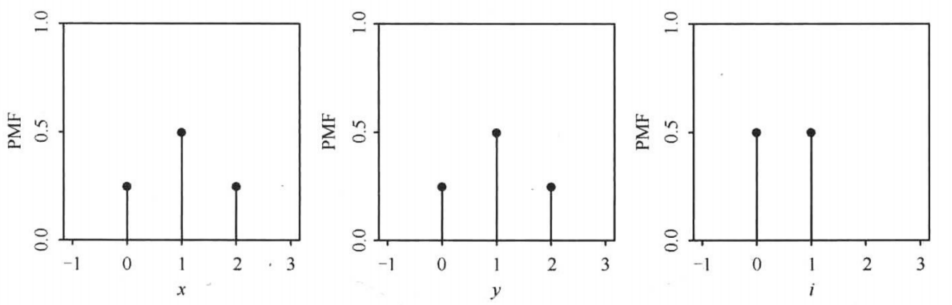
\includegraphics[width=12cm]{figures/Fig3.3.png}
	\end{figure}
\end{frame}

\begin{frame}{}
	\begin{exam}
		掷两颗骰子,其样本空间 $\Omega$ 含有 36 个等可能的样本点
		\begin{eqnarray*}
			\Omega=\{(x,y):x,y=1,2,\cdots,6\}
		\end{eqnarray*}
		令 $X$ 和 $Y$ 表示每个骰子分别出现的点数。试求下面随机变量的分布列: % 在 $\Omega$ 上定义如下三个随机变量,请给出其概率分布列
		\begin{enumerate}[<+-|alert@+>]
			\item $T_1:=X+Y=\mbox{骰子点数之和}$;
			\item $T_2:=14-(X+Y)$;
			\item $T_3:=\mbox{点数为 6 点的骰子的个数}$;
			\item $T_4:=\max\{X, Y\}=\mbox{骰子的最大点数}$
		\end{enumerate}

	\end{exam}
\end{frame}

\begin{frame}
	\begin{itemize}[<+-|alert@+>]
		\item $T_1, T_2$ 的概率分布列为 \pause
		      \begin{eqnarray*}
			      \left(\begin{array}{ccccccccccc}
				      2            & 3            & 4            & 5            & 6            & 7            & 8            & 9            & 10           & 11           & 12           \\
				      \frac{1}{36} & \frac{2}{36} & \frac{3}{36} & \frac{4}{36} & \frac{5}{36} & \frac{6}{36} & \frac{5}{36} & \frac{4}{36} & \frac{3}{36} & \frac{2}{36} & \frac{1}{36}
			      \end{array}\right)
		      \end{eqnarray*}
		      \pause
		      \begin{figure}[图 3.4.png]
			      \centering
			      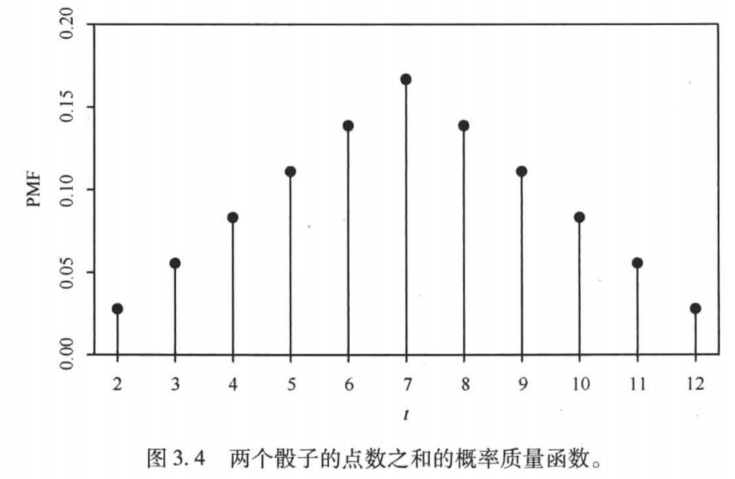
\includegraphics[width=9cm]{figures/Fig3.4.png}
		      \end{figure}

	\end{itemize}

\end{frame}

\begin{frame}
	\begin{itemize}[<+-|alert@+>]

		\item $T_3$ 的概率分布列为 \pause
		      \begin{eqnarray*}
			      \left(\begin{array}{ccc}
				      0             & 1             & 2            \\
				      \frac{25}{36} & \frac{10}{36} & \frac{1}{36}
			      \end{array}\right)
		      \end{eqnarray*}

		\item $T_4$ 的概率分布列为 \pause
		      \begin{eqnarray*}
			      \left(\begin{array}{cccccc}
				      1            & 2            & 3            & 4            & 5            & 6             \\
				      \frac{1}{36} & \frac{3}{36} & \frac{5}{36} & \frac{7}{36} & \frac{9}{36} & \frac{11}{36}
			      \end{array}\right)
		      \end{eqnarray*}
	\end{itemize}

\end{frame}

% \begin{frame}
%   \begin{exam}
%     设离散型随机变量的 $X$ 分布列为
%     \begin{eqnarray*}
%       \left(\begin{array}{ccc}
%               -1  &2 &3\\
%               0.25 & 0.5 & 0.25
%             \end{array}\right)
%     \end{eqnarray*}
%     试求 $P (X\le 0.5), P (1.5<X\le 2.5)$, 并写出 $X$ 的分布函数.
%   \end{exam}

%   \jieda $$P(X\le 0.5)=P(X=-1)=0.25,$$ $$P(1.5<X\le 2.5)=P(X=2)=0.5.$$

%   其分布函数为 \pause
%   \begin{eqnarray*}
%     F(x)=\left\{
%     \begin{array}{ll}
%       \pause  0, &  x<-1\\  \pause
%       \pause 0.25,& -1\le x<2\\  \pause
%       \pause  0.25+0.5=0.75,&  2\le x<3\\  \pause
%       \pause  0.25+0.5+0.25, & x\ge 3 \pause
%     \end{array}\right.
%   \end{eqnarray*}

% \end{frame}




\begin{frame}
	\frametitle{连续型随机变量}
	\begin{defi}[连续型随机变量] 设 $X$ 为一随机变量,$F (x)$ 为随机变量 $X$ 的分布函数,如果存在非负可积函数 $p (x)$ 使得
		\begin{eqnarray}\label{eq:contrvdist}
			F(x)=\int_{-\infty}^xp(y)dy
		\end{eqnarray}
		则称 $X$ 为连续型随机变量,其分布函数称之为连续型分布函数,函数 $p (x)$ 称为 $X$ 的概率密度函数,简称密度函数或密度.
	\end{defi}
	\pause
	\begin{rmk}
		\begin{itemize}[<+-|alert@+>]
			\item 能够表为 \eqref{eq:contrvdist} 式变上限积分的函数 $F (x)$ 在分析中称为绝对连续函数。绝对连续函数必为连续函数.
			\item 在若干个点上或零测集上改变密度函数 $p (x)$ 的值并不影响其积分的值,从而不影响分布函数 $F (x)$ 的值,这意味着连续分布的密度函数不唯一.
		\end{itemize}
	\end{rmk}

\end{frame}

\begin{frame}
	\frametitle{密度函数的性质}
	容易验证,随机变量 $X$ 的密度函数有以下性质
	\begin{enumerate}[<+-|alert@+>]
		\item 非负性:$p (x)\ge 0$;
		\item 正则性:$\int_{-\infty}^\infty p (x) dx=1$.
	\end{enumerate}

\end{frame}


\begin{frame}
	\frametitle{连续型随机变量的一些常见性质}
	\begin{itemize}
		\item $p(x)=F^\prime (x)$;
		\item $P(a< X\le b)=F(b)-F(a)=\int_a^bp(x)dx$;
		\item $0\le P (X=a)\le P (X\in (a-\epsilon,a))=\int_{a-\epsilon}^ap (x) dx\stackrel{\epsilon\rightarrow 0}{\longrightarrow} 0$, 故 $P (X=a)=0$,即连续型随机变量取值单点的概率为 0;
		\item $P(a<X\le b)=P(a\le X<b)=P(a\le X\le b)=P(a<X<b)$;
		\item 对任意的 Borel 集 $B$,
		      \begin{eqnarray*}
			      P(X\in B)=\int_Bp(x)dx
		      \end{eqnarray*}
		\item $P(X\in[x,x+\Delta x])=\int_x^{x+\Delta x}p(y)dy=p(\xi)\Delta x\approx p(x)\Delta x$
	\end{itemize}
\end{frame}
% \begin{frame}
%   \begin{exam}
%     向区间 $(0,a)$ 上任意投点,用 $X$ 表示这个点的坐标。设该点落在 $(0,a)$ 中任一小区间的概率与这个小区间的长度成正比,而与小区间的位置无关。求 $X$ 的分布函数及密度函数.
%   \end{exam}

%   \pause
%   \jieda 记 $X$ 的分布函数为 $F (x)$, 则
%   \begin{itemize}[<+-|alert@+>]
%   \item 当 $x<0$ 时,$\{X\le x\}$ 为不可能事件,故 $F (x)=P (X\le x)=0$;
%   \item 当 $x\ge a$ 时,$\{X\le x\}$ 是必然事件,故 $F (x)=P (X\le x)=1$;
%   \item 当 $x\in [0,a)$ 时, 有 $F (x)=P (X\le x)=P (0\le X\le x)=kx$, 其中 $k$ 为比例系数.
%   \item 注意到 $1=F (a)=P (0\le X\le a)=ka$, 故 $k=1/a$
%   \end{itemize}
%   \pause
%   故 $X$ 的分布函数为
%   \pause
%   \begin{eqnarray*}
%     F(x)=\left\{
%     \begin{array}{ll}
%       0,& x<0\\
%       x/a, & 0\le x<a\\
%       1,& x\ge a
%     \end{array}
%           \right.
%   \end{eqnarray*}
% \end{frame}
% \begin{frame}
%   下面我们求 $X$ 的密度函数,
%   \begin{itemize}
%   \item 当 $x<0$ 或 $x>a$ 时, $p (x)=F^\prime (x)=0$;
%   \item 当 $0<x<a$ 时,$p (x)=F^\prime (x)=1/a$;
%   \item 当 $x=0,a$ 时,$p (x)$ 可取任意值,一般就近取值为宜,不会影响概率的计算.
%   \end{itemize}
%   故 $X$ 的密度函数为
%   \begin{eqnarray*}
%     p(x)=\left\{
%     \begin{array}{ll}
%       1/a,&0<x<a,\\
%       0,&\mbox{其他}.
%     \end{array}
%           \right.
%   \end{eqnarray*}
%   其密度函数也可取为
%   \begin{eqnarray*}
%     p(x)=\left\{
%     \begin{array}{ll}
%       1/a,&0\le x\le a,\\
%       0,&\mbox{其他}.
%     \end{array}
%           \right.
%   \end{eqnarray*}

% \end{frame}

% \begin{frame}
%   \begin{exam}
%     某种型号电子元件的寿命 $X$(以小时计) 具有以下概率密度函数
%     \begin{eqnarray*}
%       p(x)=\left\{
%       \begin{array}{ll}
%         k/x^2,&x>1000,\\
%         0,&\mbox{其他}.
%       \end{array}
%             \right.
%     \end{eqnarray*}
%     其中 $k$ 为未知常数。现有一大批此种元件 (设各元件工作相互独立),问
%     \begin{enumerate}
%     \item 任取 1 只,其寿命大于 1500 小时的概率是多少?
%     \item 任取 4 只,4 只寿命都大于 1500 小时的概率是多少?
%     \item 任取 4 只,至少有一只寿命大于 1500 小时的概率是多少?
%     \item 若已知一只元件寿命大于 1500 小时,则该元件寿命大于 2000 小时的概率是多少?
%     \end{enumerate}

%   \end{exam}
% \end{frame}

\begin{frame}
	\begin{exam}
		定义函数 $F (x)$ 如下
		\begin{eqnarray*}
			F(x)=\left\{
			\begin{array}{ll}
				0,              & x< 0,      \\
				\dfrac{1+x}{2}, & 0\le x< 1, \\
				1,              & x\ge 1.
			\end{array}
			\right.
		\end{eqnarray*}
		试说明  \begin{enumerate}
			\item $F (x)$ 为分布函数;
			\item $F (x)$ 既非离散型也非连续型分布;
			\item $F (x)$ 可分解为
			      \begin{eqnarray*}
				      F(x)=\frac{1}{2}F_1(x)+\frac{1}{2}F_2(x)
			      \end{eqnarray*}
			      \pause  其中 \begin{eqnarray*}
				      F_1(x)=\left\{
				      \begin{array}{ll}
					      0, & x< 0,    \\
					      1, & x\ge 0.
				      \end{array}
				      \right.
				      \quad  F_2(x)=\left\{\begin{array}{ll}
					      0, & x<0,       \\
					      x, & 0\le x< 1, \\
					      1, & x\ge 1.
				      \end{array}
				      \right.
			      \end{eqnarray*}
		\end{enumerate}

	\end{exam}
\end{frame}


\begin{frame}
	\frametitle{勒贝格分解}
	\begin{thm}[勒贝格分解] 对任一分布函数 $F (x)$ 有如下分解
		\begin{eqnarray*}
			F(x)=c_1F_1(x)+c_2F_2(x)+c_3F_3(x),
		\end{eqnarray*}
		其中常数 $c_1,c_2,c_3\ge 0, c_1+c_2+c_3=1,$ 而 $F_1 (x),F_2 (x),F_3 (x)$ 都是分布函数,$F_1 (x)$ 为纯跳跃函数,$F_2 (x)$ 为绝对连续函数,$F_3 (x)$ 为奇异函数.
	\end{thm}
	\vspace{0.3cm}
	\pause
	\begin{itemize}[<+-|alert@+>]
		\item 上述定理中奇异函数的含义及定理的证明可参见一般的实变函数论教科书,这里我们不再详述,仅指出几种特殊情况:
		      \begin{itemize}
			      \item 在分解式中取 $c_1=1,c_2=c_3=0$ 便得到我们所讨论的离散型分布函数;
			      \item 在分解式中取 $c_2=1,c_1=c_3=0$ 便得到连续型分布函数;
			      \item 若取 $c_3=0, c_1\neq 0, c_2\neq 0, c_1+c_2=1$ 便得到离散与连续混合分布
		      \end{itemize}
		\item 从上面分析可看出,随机变量除了离散型与连续型外还有很多其他类型.
	\end{itemize}

\end{frame}



 \title[概率论]{第九讲:常见的离散型随机变量}
\institute[东南大学数学学院]{\large \textrm{Email: xzhangseu@seu.edu.cn} \\ \quad  \\
	\large 东南大学 \quad 数学学院 \\
	\vspace{0.3cm}
	%  \trc{公共邮箱: \textrm{zy.prob@qq.com}\\
	%    \hspace{-1.7cm}  密 \qquad 码: \textrm{seu!prob}}
}
\date{}


{ \setbeamertemplate{footline}{}
	\begin{frame}
		\titlepage
	\end{frame}
}
% \begin{CJK*}{GBK}{song}

%   \title{简单随机抽样}
%   \author{林语堂}
%   \institute{University}
%   \date{2009-03-31}
%   \date{}
%   \begin{frame}
%     \titlepage
%   \end{frame}

%   \begin{frame}
%     \frametitle{第二章:简单随机抽样}
%     \tableofcontents
%   %     You might wish to add the option[pausesections]
%   \end{frame}

%   \AtBeginSubsection[]{
%   \begin{frame}<beamer>
%     \frametitle{Outline}
%     \tableofcontents[currentsection,currentsubsection]
%   \end{frame}
% }
%   定义目录页



% \begin{frame}[plain]
%   \frametitle{目录}
%   \setcounter{tocdepth}{2}
%   \tableofcontents
% \end{frame}
\addtocounter{framenumber}{-3}  % 目录页不计算页码
%\section{随机变量}
\subsection{伯努利试验及其离散型分布}
\begin{frame}
	\frametitle{伯努利实验}
	\begin{itemize}[<+-|alert@+>]
		\item 只有两种可能结果的试验称为伯努利试验;例如抽检产品,可能是合格品,也可能是次品;掷两颗骰子,可能得到同点,也可能得到不同点,等等都是伯努利试验.
		\item 伯努利试验的样本空间 $\Omega$ 并不一定只含有两个样本点,有时只是把我们所关心的一部分样本点归结为一种结果 $A$, 同时把其余的样本点的集合看作另一种结果 $\bar{A}$;
		\item 在上述掷骰子的试验中,样本空间 $\Omega$ 共含有 36 个样本点,如果我们只关心同点是否发生,就可以把其中的 6 个样本点组成的事件 $A:=\{(i,i):i=1,\cdots, 6\}$ 视为一种结果,而其余的 30 个样本点组成另一结果 $\bar{A}:=\{\mbox{不同点}\}$;
		\item 此外我们不再关心由 $\Omega$ 的其他非空子集组成的事件,于是对于伯努利试验而言,事件 $\sigma$ 代数应取为 $\mathcal{F}=\{\emptyset, A, \bar{A}, \Omega\}$;
		\item 通常把结果 $A$ 称作 "成功", 而把 $\bar{A}$ 称作 "失败";
		\item 再取定成功失败的概率 $p=P (A), q=P (\bar{A})$ ($p>0,q>0$ 且 $p+q=1$), 则建立了一次伯努利试验的概率空间 $(\Omega,\mathcal{F},P)$.
	\end{itemize}
\end{frame}
\begin{frame}
	\begin{itemize}[<+-|alert@+>]
		\item 在概率论的理论与应用中,经常以一系列独立重复的伯努利试验作为概率模型;
		\item 所谓重复,粗略的说即各次试验的概率空间都是上述的 $(\Omega,\mathcal{F},P)$;
		\item 而 $n$ 个试验的独立性则是指各次试验的结果互不影响,即对于第 $i$ 次试验的任何结果 $E_i (i=1,\cdots, n)$ 均有
		      \begin{eqnarray*}
			      P(E_1E_2\cdots E_n)=P(E_1)P(E_2)\cdots P(E_n)
		      \end{eqnarray*}
		\item 将一次伯努利试验独立重复 $n$ 次,称作 $n$ 重伯努利试验;
		\item 将一次伯努利试验独立地重复下去所得到的一系列试验,称为可列重伯努利试验.
	\end{itemize}
\end{frame}

\begin{frame}
	\frametitle{二项分布:$n$ 重伯努利试验中成功的次数 $X$}
	\begin{itemize}[<+-|alert@+>]
		\item $X$:$n$ 重伯努利试验中成功 (事件 $A$ 发生) 的次数;
		\item $X$ 的所有可能取值为: $0, 1, \cdots, n$;
		\item 下面我们考虑 $X$ 的分布列
		      \begin{itemize}
			      \item $n$ 重伯努利试验的样本空间: $\Omega:=\{\omega=(\omega_1,\cdots,\omega_n):\omega_i\mbox{或者为} A\mbox{或者为}\bar{A}\}$
			      \item 样本空间样本点的个数为 $2^n$ 个;
			      \item $\{X=k\}=\{\omega=(\omega_1,\cdots,\omega_n):\omega_1,\cdots,\omega_n\mbox{中有} k\mbox{个} A\}$, 共包含 $C_n^k$ 个样本点;
			      \item 若任给样本点 $\omega=(\omega_1,\cdots,\omega_n)\in \{X=k\}$, 则意味着 $\omega_1,\cdots,\omega_n$ 中有 $k$ 个 $A$, $n-k$ 个 $\bar{A}$, 故由独立性可知
			            \begin{eqnarray*}
				            P(\omega)=p^k(1-p)^{n-k}
			            \end{eqnarray*}
			      \item 而事件 $\{X=k\}$ 中共有 $C_n^k$ 个类似的 $\omega$, 故
			            \begin{eqnarray*}
				            P(X=k)=C_n^kp^k(1-p)^{n-k}:=b(k;n,p), k=0,1,\cdots, n
			            \end{eqnarray*}
			            这个分布常称为二项分布,记为 $X\sim B (n,p)$.
			      \item 容易验证,$\sum_{k=0}^nC_n^kp^k (1-p)^{n-k}=(p+1-p)^n=1$
		      \end{itemize}
	\end{itemize}

\end{frame}
\begin{frame}
	\frametitle{两点分布}
	\begin{itemize}
		\item $n=1$ 时的二项分布 $B (1,p)$ 称为二点分布,或 $0-1$ 分布,或称伯努利分布,其分布列为
		      \begin{eqnarray*}
			      P(X=k)=p^k(1-p)^{1-k}, k=0, 1
		      \end{eqnarray*}
		      或记为
		      \begin{eqnarray*}
			      \left(\begin{array}{cc}
				      0,   & 1  \\
				      1-p, & p
			      \end{array}\right)
		      \end{eqnarray*}
		\item $B (1,p)$ 主要用于描述一次伯努利试验中成功的次数 (0 或 1);
		\item 若记 $X_i$ 表示第 $i$ 次伯努利试验中成功的次数,则 $X_i$ 相互独立且有
		      \begin{eqnarray*}
			      X=X_1+X_2+\cdots X_n
		      \end{eqnarray*}
		      即二项分布随机变量可写为 $n$ 个独立同为两点分布随机变量的和.
	\end{itemize}
\end{frame}
\begin{frame}
	\frametitle{二项分布的性质}
	\begin{itemize}[<+-|alert@+>]
		\item 对 $k\ge 1$, 考虑比值
		      \begin{eqnarray*}
			      \dfrac{b(k;n,p)}{b(k-1;n,p)}&=&\pause \dfrac{C_n^kp^k(1-p)^{n-k}}{C_n^{k-1}p^{k-1}(1-p)^{n-k+1}}=\pause \dfrac{(n-k+1)p}{k(1-p)}\\
			      &=&\pause \dfrac{k(1-p)+(n+1)p-k}{k(1-p)}=\pause 1+\dfrac{(n+1)p-k}{k(1-p)}
		      \end{eqnarray*}
		\item 当 $(n+1) p>k$ 时,$b (k;n,p)>b (k-1;n,p)$;
		\item 当 $(n+1) p<k$ 时,$b (k;n,p)<b (k-1;n,p)$;
		\item 从而,对于固定的 $n,p$,$\{X=k\}$ 的概率 $b (k;n,p)$ 先随 $k$ 增大而增大,再随 $k$ 增大而减小,故必有最大值:
		      \begin{itemize}
			      \item 如果 $m:=(n+1) p$ 为整数,则 $b (m;n,p)=b (m-1;n,p)$ 同为 $b (k;n,p)$ 的最大值
			      \item 如果 $(n+1) p$ 不为整数,则 $b (k;n,p)$ 在 $m=[(n+1) p]$ 处取到最大值 (此处 $[a]$ 表示不超过 $a$ 的最大整数)
		      \end{itemize}
		\item 我们称使得 $b (k;n,p)$ 取得最大值的 $m$ 为二项分布随机变量的最可能值,或称为 $n$ 重伯努利试验中最可能的成功次数.
	\end{itemize}
\end{frame}


\begin{frame}{二项分布的性质}
	\begin{thm}\label{338} 设 $X\sim B (n,p)$, 且 $q=1-p$(通常用 $q$ 表示伯努利试验失败的概率), 则有 $n-X\sim B (n,q)$.
	\end{thm}

	\pause
	% \begin{jieda}
	\begin{itemize}[<+-|alert@+>]
		\item 借用二项分布的直观定义:将 $X$ 为 $n$ 次独立伯努利试验成功的次数,则 $n-X$ 为这些试验中失败的次数.
		\item 互相交换成功与失败的角色,可知 $n-X\sim B (n,q)$.
		\item 也可从分布列 (概率质量函数) 的角度出发得到
		      $n-X\sim B(n,q).$
		\item 令 $Y=n-X$, 则 $Y$ 的分布列 (概率质量函数) 为 \pause
		      \begin{equation*}
			      \begin{aligned}
				      P(Y=k)= & P(n-X=k)=P(X=n-k)                                                           \\
				      =       & \left(\begin{matrix}
						                      n   \\
						                      n-k \\
					                      \end{matrix}\right)p^{n-k}q^{k}=\left(\begin{matrix}
						                                                            n \\
						                                                            k \\
					                                                            \end{matrix}\right)q^kp^{n-k},
			      \end{aligned}
		      \end{equation*}
	\end{itemize}
	% \end{jieda}
\end{frame}

\begin{frame}{二项分布的性质}

	\begin{thm} 设 $X\sim B (n,p)$, 其中 $n$ 为偶数,$p=1/2$, 则 $X$ 的分布关于 $n/2$ 对称,即对任意的非负整数 $j$, 均有
		$$P(X=\frac{n}{2}+j)=P(X=\frac{n}{2}-j).$$
	\end{thm}
	\pause
	%\vspace{0.2cm}

	\begin{jieda} 由定理 \ref{338} 可知,$n-X$ 同样服从 $B (n,1/2)$. \pause 因此对任意非负整数 $k$ 均有
		$$P(X=k)=P(n-X=k)=P(X=n-k).$$
		\pause
		令 $k=n/2+j$, 即可得证. % 得推论 \ref{338} 的结果。该推论也解释了为什么图 3.6 中 $Bin (10,1/2)$ 是关于 5 对称的.
	\end{jieda}

	%\begin{exam}({\tc 掷硬币续}) 回顾例 \ref{312}, 现在已经知道 $X\sim Bin (2,1/2),Y~\sim Bin (2,1/2)$ 和 $I\sim Bern (1/2)$. 由定理 \ref{337} 可知,$X$ 和 $Y=2-X$ 具有相同的分布。再根据推论 \ref{338}, 得到 $X$ 的分布 (以及 $Y$ 的分布) 是关于 1 对称的.
	%\end{exam}
\end{frame}






\begin{frame}
	\vspace{0.4cm}
	\begin{exam}
		设每台自动机床在运行过程中需要维修的概率均为 $p=0.01$, 并且各机床是否需要维修相互独立。如果:
		\begin{enumerate}
			\item 每名维修工人负责看管 20 台机床;
			\item 3 名维修工人负责看管 80 台机床;
		\end{enumerate}
		求机床不能及维修的概率.
	\end{exam}

	\pause \jieda 1. 这是 $n=20$ 重伯努利试验,参数 $p=0.01$, 故需要维修的机床数 $X$ 服从 $B (20,0.01)$ 分布。故不能及时维修的概率为 \pause
	\begin{eqnarray*}
		P(X>1)&=&\pause 1-P(X\le 1)=\pause 1-P(X=0)-P(X=1)\\
		&=&\pause 1-C_{20}^00.01^0(1-0.01)^{20}-C_{20}^10.01(1-0.01)^{20-1}\approx 0.0169
	\end{eqnarray*}
	\pause 2. 此时需要维修的机床数 $X$ 服从 $B (80,0.01)$ 分布,类似可得不能及时维修的概率为
	\begin{eqnarray*}
		P(X>3)=1-\sum_{k=0}^3b(k;80,0.01)\approx 0.0087
	\end{eqnarray*}

\end{frame}

\begin{frame}
	\frametitle{小概率事件终将发生}
	\begin{exam}
		在可列重伯努利试验中,求事件 $E:=\{\mbox{试验终将成功}\}$ 的概率.
	\end{exam}
	\pause

	\jieda 考虑所求概率事件的反面即 $\overline{E}:=\{\mbox{试验永不成功}\}$.\pause 若我们记
	\begin{eqnarray*}
		F_n:=\{\mbox{前} n\mbox{次试验均失败}\},
	\end{eqnarray*}
	\pause
	则易知,$\{F_n\}$ 为单调下降事件序列,且
	\begin{eqnarray*}
		\lim_{n\rightarrow \infty}F_n=\pause \cap_{n=1}^\infty F_n=\pause \overline{E}
	\end{eqnarray*}
	\pause 从而
	\begin{eqnarray*}
		P(\overline{E})=\pause P(\lim_{n\rightarrow\infty}F_n)=\pause \lim_{n\rightarrow\infty }P(F_n)=\pause \lim_{n\rightarrow\infty }C_n^0p^0(1-p)^n=\pause 0
	\end{eqnarray*}
	\pause 故
	\begin{eqnarray*}
		P(E)=1-P(\overline{E})=1-0=1
	\end{eqnarray*}
	\pause 无论成功的概率有多小,但是试验最终成功的概率为 1, 也就是说小概率事件终将发生的概率为 1.
\end{frame}

%   \title[概率论]{第十一讲:常见的离散型随机变量 (II)}
%   \author[张鑫 {\rm Email: x.zhang.seu@foxmail.com} ]{\large 张 鑫}
%   \institute[东南大学数学学院]{\large \textrm{Email: x.zhang.seu@foxmail.com} \\ \quad  \\
%   	\large 东南大学 \quad 数学学院 \\
%   	\vspace{0.3cm}
%   	%  \trc{公共邮箱: \textrm{zy.prob@qq.com}\\
%   		%    \hspace{-1.7cm}  密 \qquad 码: \textrm{seu!prob}}
%   }
%   \date{}



%   	{ \setbeamertemplate{footline}{}
%   		\begin{frame}
%   			\titlepage
%   		\end{frame}
%   	}

%   	% \begin{frame}[plain]
%   		%   \frametitle{目录}
%   		%   \setcounter{tocdepth}{2}
%   		%   \tableofcontents
%   		% \end{frame}
%   	\addtocounter{framenumber}{-3}  % 目录页不计算页码
%   	\section{随机变量}
%   	\subsection{伯努利试验及其离散型分布}

\begin{frame}
	\frametitle{几何分布:可列重伯努利试验中首次成功的等待时间 $X$}
	\begin{itemize}[<+-|alert@+>]
		\item 记 $X$ 为可列重伯努利试验中首次成功的等待时间即首次成功所需要试验的次数;
		\item $\{X=k\}=\{\underbrace{\overline{A}\cdots \overline{A}}_{k-1\mbox{个}} A\}$, 故
		      \begin{eqnarray*}
			      P(X=k)=(1-p)^{k-1}p:=g(k;p), k=1,\cdots,
		      \end{eqnarray*}
		      这个分布常称为几何分布,记为 $X\sim G (p)$.
	\end{itemize}
\end{frame}
\begin{frame}
	\frametitle{几何分布的性质}
	\begin{thm}
		取值自然数的随机变量 $X$ 为几何分布当且仅当 $X$ 有无记忆性:
		\begin{eqnarray}\label{eq:memory}
			P (X>m+n|X>m)=P (X>n), \mbox{对任意的} m,n \ge 1.
		\end{eqnarray}
	\end{thm}
	\zheng 若 $X$ 为几何分布,则
	\begin{eqnarray*}
		P(X>m+n|X>m)=\pause \dfrac{P(X>m+n,X>m)}{P(X>m)}=\pause \dfrac{P(X>m+n)}{P(X>m)}
	\end{eqnarray*}
	\pause 而
	\begin{eqnarray*}
		P(X>n)=\pause \sum_{k=n+1}^\infty (1-p)^{k-1}p=\pause \dfrac{(1-p)^{n}p}{1-(1-p)}=\pause (1-p)^n
	\end{eqnarray*}
	\pause 故
	\begin{eqnarray*}
		P(X>m+n|X>m)=\dfrac{(1-p)^{m+n}}{(1-p)^m}=(1-p)^n=P(X>n)
	\end{eqnarray*}

\end{frame}

\begin{frame}
	\vspace{0.5cm}
	若 $X$ 具有无记忆性,则由~\eqref{eq:memory} 知
	\pause \begin{eqnarray*}
		Q_n:=P (X>n)>0, \quad \mbox{对任意的} n\ge 1
	\end{eqnarray*}
	\pause 并且有
	\begin{eqnarray*}
		Q_{m+n}=P(X>m+n)=\pause P(X>m)P(X>m+n|X>m)=\pause Q_mQ_n
	\end{eqnarray*}
	\pause 从而 \vspace{-0.7cm}
	\begin{eqnarray*}
		Q_m=Q_1^m
	\end{eqnarray*}
	\pause 注意到 $Q_1\in (0,1)$, 事实上,
	\begin{itemize}[<+-|alert@+>]
		\item $Q_1=P (X>1)>0$ 显然;
		\item  若 $Q_1=1$, 则对一切的 $m$ 均有 $Q_m=P (X>m)=1$, 这与 $X$ 取自然数矛盾,故 $Q_1\in (0,1)$.
	\end{itemize}
	\pause 故取 $p=1-Q_1\in (0,1)$, 且对任意的 $k\ge 1$ 有
	\begin{eqnarray*}
		P(X=k)&=&\pause P(X>k-1)-P(X>k)=\pause Q_{k-1}-Q_k\\
		&=&\pause (1-p)^{k-1}-(1-p)^k=\pause (1-p)^{k-1}p
	\end{eqnarray*}

\end{frame}

\begin{frame}
	\frametitle{无记忆性}
	\begin{eqnarray*}
		P(X>m+n|X>m)=P(X>n)
	\end{eqnarray*}
	\begin{itemize}[<+-|alert@+>]
		\item 上述的无记忆性表明:已知试验了 $m$ 次未获得成功,再加做 $n$ 次试验仍不成功的概率,等于从开始算起做 $n$ 次试验都不成成功的概率.
		\item 换句话放,已做过的 $m$ 次失败的试验被忘记了;
		\item 产生几何分布的这种无记忆性的根本原因在于,我们进行的是独立重复试验,这是不学习,不总结经验的试验,已经做过的试验当然不会留下记忆.
	\end{itemize}
\end{frame}

\begin{frame}
	\vspace{0.3cm}
	\begin{exam}
		10 把外形相同的钥匙中只有一把能打开门。现一一试开,试对每次试毕放回与不放回两种情形,分别求事件 $E:=\{\mbox{至多试} 3\mbox{次能打开门}\}$ 的概率.
	\end{exam}

	\pause
	\jieda 1. 放回情形是独立重复试验,属伯努利概型。以 $X$ 表示首次打开门的等待时间,则 $X$ 服从几何分布 $G (0.1)$. 故所求概率为
	\begin{eqnarray*}
		P(E)=P(X\le 3)=\sum_{k=1}^3(1-0.1)^{k-1}0.1=0.271
	\end{eqnarray*}
	\pause
	2. 不放回情形不再是独立重复试验,适用于古典概型。样本点总数 $n (\Omega)=C_{10}^3$, 而 $n (\overline{E})=C_9^3$. 故
	\begin{eqnarray*}
		P(E)=1-P(\overline{E})=1-\dfrac{C_9^3}{C_{10}^3}=0.3
	\end{eqnarray*}
	\pause 或令 $A_i:=\{\mbox{第} i\mbox{次取到能开门的钥匙}\}$, 则 $A_1,A_2,A_3$ 互不相容,由可加性及抽签的公平性可得
	\begin{eqnarray*}
		P(E)=P(\cup_{i=1}^3A_i)=\sum_{i=1}^3P(A_i)=0.3
	\end{eqnarray*}

\end{frame}
\begin{frame}
	\frametitle{帕斯卡 (Pascal) 分布:第 $r$ 次成功的等待时间}
	\begin{itemize}[<+-|alert@+>]
		\item 记 $X_r$ 为可列重伯努利试验中第 $r$ 次成功的等待时间即第 $r$ 次成功所需要试验的次数;
		\item 易见 $X$ 的所有可能取值为 $k=r, r+1,\cdots, $ 并且有
		      \begin{eqnarray*}
			      \{X_r=k\}&=&\{\mbox{前} k-1\mbox{次试验恰有} r-1\mbox{次成功且第} k\mbox{次成功}\}\\
			      \pause
			      P (X_r=k)&=&\pause P (\mbox{前} k-1\mbox{次试验恰有} r-1\mbox{次成功}) P (\mbox{第} k\mbox{次成功})\\
			      &=&\pause C_{k-1}^{r-1}p^{r-1}(1-p)^{k-1-(r-1)}p\\
			      &=&\pause C_{k-1}^{r-1}p^r(1-p)^{k-r}:=f(k;r,p), \quad k=r, r+1,\cdots
		      \end{eqnarray*}
		      \pause 这个分布常称为帕斯卡 (Pascal) 分布或负二项分布.
		\item $f (k;r,p), k=r,r+1,\cdots,$ 可以成为离散型分布的密度,事实上: $f (k;r,p)>0$ 显然,其和
		     {\small \begin{eqnarray*}
			      \sum_{k=r}^\infty f(k;r,p)&=&\pause  \sum_{k=r}^\infty C_{k-1}^{r-1}p^r(1-p)^{k-r}\xlongequal[q=1-p]{k-r=i}\pause \sum_{i=0}^\infty C_{r+i-1}^{r-1}p^rq^{r+i-r}\\
			      &=&\pause \sum_{i=0}^\infty C_{r+i-1}^ip^rq^i=\pause \sum_{i=0}^\infty C_{-r}^ip^r(-q)^i=\pause p^r(1-q)^{-r}=1 \end{eqnarray*}
		      }
	\end{itemize}
\end{frame}
\begin{frame}
	\frametitle{帕斯卡分布的性质}
	\begin{itemize}[<+-|alert@+>]
		\item 若帕斯卡分布中的 $r=1$, 则此时的帕斯卡分布即为几何分布;
		\item 如果记 $$\tau_1=X_1, \quad \tau_n=X_n-X_{n-1}, \quad n>1, $$ 则随机变量 $\tau_n$ 是第 $n-1$ 次成功到第 $n$ 次成功的间隔时间。显然有
		      \begin{eqnarray*}
			      X_r=\tau_1+\tau_2+\cdots+\tau_r
		      \end{eqnarray*}
		\item 以后我们会看到: $\tau_1,\cdots, \tau_r$ 是 $r$ 个相互独立的随机变量且每个 $\tau_k$ 均服从几何分布.
	\end{itemize}
\end{frame}

\begin{frame}
	\begin{exam}
		某人口袋中有两盒火柴,开始时每盒各装 $n$ 根。每次他从口袋中任取一盒使用其中的一根火柴。求此人掏出一盒发现已空,而另一盒尚余 $r$ 根的概率.
	\end{exam}

	\pause
	\jieda 记
	\begin{eqnarray*}
		E=\{\mbox{掏出甲盒已空而乙盒尚余} r\mbox{根}\}
	\end{eqnarray*}
	\pause 则由对称性可知所求概率为 $2P (E)$. \pause 若我们以取出甲盒为 "成功", 这便是一个成功率 $p=1/2$ 的独立重复伯努利试验.
	\pause 而
	\begin{eqnarray*}
		E=\{\mbox{第} n+1\mbox{次成功发生在第} 2n-r+1\mbox{次试验}\}
	\end{eqnarray*}
	\pause 故所求概率为
	\begin{eqnarray*}
		2P(E)&=&\pause 2f(2n-r+1;n+1,1/2)=\pause 2C_{2n-r}^n(\dfrac{1}{2})^{n+1}(\dfrac{1}{2})^{2n-r-n}\\
		&=&\pause C_{2n-r}^n2^{r-2n}
	\end{eqnarray*}

\end{frame}


\begin{frame}
	\frametitle{分赌注问题}
	\begin{exam}
		1654 年,当时的职业赌徙 DeMere 爵士向法国的大数学家 Pascal 提出如下问题:甲乙两人各下赌注 $m$ 元,商定先胜三局者取得全部赌金。假定在每一局中二人获胜的机会相等,且各局胜负相互独立。如果当甲胜一局而乙胜零局时赌博被迫中止,问赌注如何分?
	\end{exam}
	\pause
	\begin{itemize}[<+-|alert@+>]
		\item 为解决这个问题,Pascal 与当时声望很高的数学家 Fermat 建立了通信联系。他们进行了卓有成效的讨论,不仅完满的回答了分赌注问题,而且为解决其他概率问题建立起了框架,极大的促进了概率论的建立与发展;
		\item Pascal 令人信服的指出,赌金的分法应当取决于若赌博能继续进行下去甲乙各自获胜的概率,这个概率即为在 $p=0.5$ 的可列重伯努利试验中 2 次成功发生在 3 次失败之前的概率;
		\item 更一般的,下面我们求一下 $n$ 次成功发生在 $m$ 次失败之前的概率.
	\end{itemize}
\end{frame}

\begin{frame}
	\begin{exam}
		在可列重伯努利试验中,求下面事件的概率: $$E=\{n\mbox{次成功发生在} m\mbox{次失败之前}\}$$
	\end{exam}
	\pause \jieda 记 $F_k=\{\mbox{第} n\mbox{次成功发生在第} k\mbox{次试验}\}$, 则
	\begin{eqnarray*}
		E=\cup_{k=n}^{n+m-1}F_k
	\end{eqnarray*}
	\pause 从而由 $F_k$ 的互不相容性可得
	\begin{eqnarray*}
		P(E)=\sum_{k=n}^{n+m-1}P(F_k)=\sum_{k=n}^{n+m-1}C_{k-1}^{n-1}p^n(1-p)^{k-n}
	\end{eqnarray*}
	\pause 利用上面的公式可计算 $n=2,m=3, p=1/2$ 时,其相应的概率为
	\begin{eqnarray*}
		P (\mbox{甲胜})=P (E)\xlongequal{n=2,m=3,p=1/2}\dfrac{11}{16}
	\end{eqnarray*}
	故赌注应以 $11:5$ 的比例分配给甲乙两人.
\end{frame}
\subsection{泊松分布}
\begin{frame}
	\begin{columns}
		\column{4cm}
		\begin{figure}[htbp]\nonumber
			\centering
			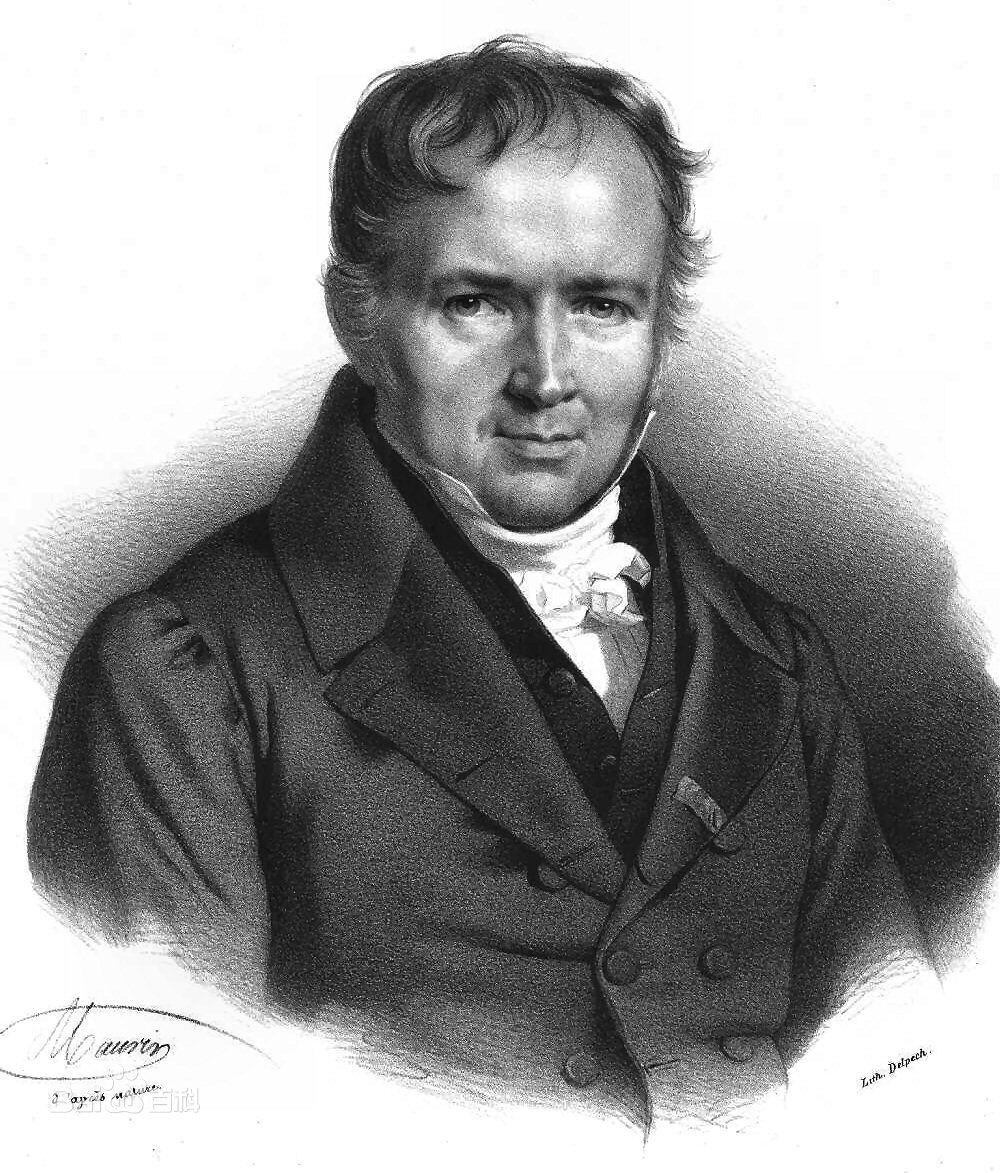
\includegraphics[width=4cm]{p1.jpg}
			\caption{泊松}
		\end{figure}
		\pause
		\column{6cm}
		\begin{itemize}[<+-|alert@+>]
			\item 西莫恩・德尼・泊松:法国数学家、几何学家和物理学家;
			      % \item 1781 年 6 月 21 日生于法国卢瓦雷省的皮蒂维耶,1840 年 4 月 25 日卒于法国索镇;
			\item 泊松的科学生涯开始于研究微分方程及其在摆的运动和声学理论中的应用;
			\item 对积分理论、行星运动理论、热物理、电磁理论、位势理论和概率论都有重要贡献;
			\item 19 世纪概率统计领域里的卓越人物,改进了概率论的运用方法,特别是用于统计方面的方法,建立了描述随机现象的一种概率分布──泊松分布;
			\item 推广了 “大数定律”,并导出了在概率论与数理方程中有重要应用的泊松积分。
		\end{itemize}


	\end{columns}
\end{frame}

\begin{frame}
	\frametitle{泊松 (Poisson) 分布}
	\begin{itemize}[<+-|alert@+>]
		\item Poisson 分布是概率论中一种重要的离散型分布,它在理论与实践中都有广泛的应用,常与单位时间 (面积) 内上的计数过程相联系;
		      \begin{itemize}
			      \item 一天内到达某商场的顾客数;
			      \item 单位时间内,电路受外界电磁波的冲击次数;
			      \item 一定时期内,某放射性物质放射出来的粒子数等
		      \end{itemize}
		\item 在二项分布中,当参数 $n$ 较大时,计算二项概率 $b (k;n,p)$ 会非常麻烦.
	\end{itemize}
	\pause  \begin{thm}
		设有一列二项分布 $\{b (k;n,p_n)\}$, 若其参数列 $p_n$ 满足
		\begin{eqnarray*}
			\lim_{n\rightarrow \infty}np_n=\lambda>0,
		\end{eqnarray*}
		则对任何非负整数 $k$ 有
		\begin{eqnarray*}
			\lim_{n\rightarrow \infty}b(k;n,p_n)=\dfrac{\lambda^k}{k!}e^{-\lambda}.
		\end{eqnarray*}
	\end{thm}
\end{frame}
\begin{frame}

	\vspace{0.4cm}
	\zheng 记 $\lambda_n:=np_n$, 则
	\begin{eqnarray*}
		b(k;n,p_n)&=&\pause C_n^kp_n^k(1-p_n)^{n-k}=\pause \dfrac{n!}{k!(n-k)!}(\dfrac{\lambda_n}{n})^k(1-\dfrac{\lambda_n}{n})^{n-k}\\
		&=&\pause \dfrac{\lambda_n^k}{k!}(1-\dfrac{1}{n})(1-\dfrac{2}{n})\cdots(1-\dfrac{k-1}{n})(1-\dfrac{\lambda_n}{n})^{n-k}
	\end{eqnarray*}
	\pause 注意到
	\begin{eqnarray*}
		&&\pause \lim_{n\rightarrow\infty}\lambda_n^k=\lambda^k, \\
		&&\pause \lim_{n\rightarrow\infty}(1-\dfrac{1}{n})(1-\dfrac{2}{n})\cdots(1-\dfrac{k-1}{n})=1\\
		&&\pause \lim_{n\rightarrow\infty}(1-\dfrac{\lambda_n}{n})^{n-k}=\pause \lim_{n\rightarrow\infty}e^{(n-k)\ln(1-\dfrac{\lambda_n}{n})}\\
		&&=\pause e^{\lim_{n\rightarrow\infty}(n-k)\ln(1-\frac{\lambda_n}{n})}=\pause e^{\lim_{n\rightarrow\infty}(n-k)(-\frac{\lambda_n}{n}+o(\frac{1}{n}))}\\
		&&=\pause e^{\lim_{n\rightarrow\infty}(-\lambda_n+\frac{k\lambda_n}{n}+(n-k)o(\frac{1}{n}))}=\pause e^{-\lambda}
	\end{eqnarray*}
	\pause 从而 \vspace{-0.8cm}
	\begin{eqnarray*}
		\lim_{n\rightarrow\infty}b(k;n,p_n)=\dfrac{\lambda^k}{k!}e^{-\lambda}, k=0, 1, 2,\cdots
	\end{eqnarray*}

\end{frame}
\begin{frame}
	有了上述定理,当 $n$ 很大而 $p$ 很小时,可以用近似公式计算二项概率
	\begin{eqnarray*}
		b(k;n,p)\approx \dfrac{(np)^k}{k!}e^{-np}
	\end{eqnarray*}
	这里我们要求 $p$ 很小,为保证 $n$ 很大时,乘积 $np$ 有适度的大小.

	\pause  \begin{defi}[泊松分布] 对参数 $\lambda>0$, 记
		\begin{eqnarray*}
			p(k;\lambda)=\dfrac{\lambda^k}{k!}e^{-\lambda}, \quad k=0, 1,\cdots.
		\end{eqnarray*}
		\pause 易见 $p (k;\lambda)>0$ 且
		\begin{eqnarray*}
			\sum_{k=0}^\infty p(k;\lambda)=\sum_{k=0}^\infty \dfrac{\lambda^k}{k!}e^{-\lambda}=\pause e^\lambda e^{-\lambda}=1
		\end{eqnarray*}
		\pause 即 $\{p (k;\lambda)\}$ 可以看成离散型分布的密度,我们就把它称为以 $\lambda$ 为参数的泊松分布,记作 $P (\lambda)$.
	\end{defi}
\end{frame}
\begin{frame}
	\frametitle{泊松分布的性质}
	\begin{itemize}[<+-|alert@+>]
		\item 泊松分布列 $p (k;\lambda)$ 随 $k$ 变化情况与二项分布相似,事实上,考虑比值
		      \begin{eqnarray*}
			      \dfrac{p(k;\lambda)}{p(k-1;\lambda)}=\dfrac{\lambda^k(k-1)!e^{-\lambda}}{\lambda^{k-1}k!e^{-\lambda}}=\dfrac{\lambda}{k}, k\ge 1
		      \end{eqnarray*}
		      \begin{itemize}
			      \item 当 $k<\lambda$ 时有,$p (k;\lambda)>p (k-1;\lambda)$;
			      \item 当 $k>\lambda$ 时有,$p (k;\lambda)<p (k-1;\lambda)$;
			      \item 因此 $p (k;\lambda)$ 随 $k$ 先升后降,在 $m=[\lambda]$ 处达到最大值,而 $\lambda$ 为整数时,$p (k;\lambda)$ 在 $m=\lambda,\lambda-1$ 处同时取到最大值.
		      \end{itemize}
		\item 泊松分布在随机选择下的不变性:假设某块放射性物质在单位时间内发射出的粒子数 $X$ 服从 $P (\lambda)$ 分布。而每个粒子被记录下来的概率为 $p$ 即粒子有 $1-p$ 的概率被计数器遗漏,如果各粒子是否被记录相互独立,试求记录下的粒子数 $Y$ 的分布.
	\end{itemize}
\end{frame}
\begin{frame}
	\begin{eqnarray*}
		P(Y=k)&=&\pause \sum_{n=0}^\infty P(X=n, Y=k)=\pause \sum_{n=0}^\infty P(X=n) P(Y=k|X=n)\\
		&=&\pause \sum_{n=k}^\infty P(X=n) P(Y=k|X=n)=\pause \sum_{n=k}^\infty p(n;\lambda)B(k;n,p) \\
		&=&\pause \sum_{n=k}^\infty \dfrac{\lambda^n}{n!}e^{-\lambda}C_n^kp^k(1-p)^{n-k}=\pause \sum_{n=k}^\infty\dfrac{[\lambda(1-p)]^{n-k}}{(n-k)!}\dfrac{1}{k!}e^{-\lambda}(\lambda p)^k\\
		&=&\pause \dfrac{1}{k!}e^{-\lambda p}(\lambda p)^k\\
	\end{eqnarray*}
\end{frame}

\subsection{超几何分布}

\begin{frame}{超几何分布}
	假设某个罐子中有 $w$ 个白球和 $b$ 个黑球,考虑如下两种取球方式
	\begin{itemize}[<+-|alert@+>]
		\item 有放回的抓取 $n$ 个球
		      \begin{itemize}[<+-|alert@+>]
			      \item $X:=n$ 个球中白球的数量;
			            \vspace{0.1cm}
			      \item $X\sim B(n, \dfrac{w}{w+b})$
		      \end{itemize}

		\item 不放回的抓取 $n$ 个球
		      \begin{itemize}[<+-|alert@+>]
			      \item $X:=n$ 个球中白球的数量;
			      \item $X$ 服从超几何分布,记为 $X\sim H (w,b,n)$;
			      \item 易知
			            $$P(X=k)=\frac{C_w^kC_b^{n-k}}{C_{w+b}^n}:=h(k,w,b,n), k=0,1,\cdots,r,$$
			            其中 $r:=\min\{w,n\}$.
			      \item 若要验证以上给出的确实为一个概率分布列,只需注意到下面的组合等式成立
			            \begin{eqnarray*}
				            \sum_{k=0}^rC_w^kC_{b}^{n-k}=C_{w+b}^n
			            \end{eqnarray*}
		      \end{itemize}

	\end{itemize}
\end{frame}




\begin{frame}{超几何分布:两个例子}
	\begin{itemize}[<+-|alert@+>]
		\item 不合格品抽检问题
		      \begin{itemize}[<+-|alert@+>]
			      \item 设有 $N$ 件产品,其中有 $M$ 件不合格品,从中不放回的抽取 $n$ 件;
			      \item 令 $X:=n$ 件抽取的产品中不合格品的件数;
			      \item $X\sim H(M,N-M,n)$
		      \end{itemize}
		\item 麋鹿的捕获 - 再捕获问题
		      \begin{itemize}[<+-|alert@+>]
			      \item 森林中共有 $N$ 头麋鹿。某天,捕获了 $M$ 头麋鹿,标记后将这 $M$ 头麋鹿再放回野外.
			      \item 几天后,又重新随机地捕获 $n$ 头麋鹿。假设重新捕获的麋鹿也同样可能是之前捕获的麋鹿.
			      \item 令 $X:=$ 再次被捕获的麋鹿的数量;
			      \item $X\sim H(M,N-M,n)$;
			      \item 第一次捕获的 $M$ 头麋鹿相当于前面例子中白球的总数,第一次未捕获的 $N-M$ 头麋鹿相当于前面例子中黑球的总数,再次被捕获的 $n$ 头麋鹿相当于前面例子中抽样的数量.
		      \end{itemize}
	\end{itemize}
\end{frame}




\begin{frame}{超几何分布的适用基础}
	\begin{itemize}[<+-|alert@+>]
		\item 除上面例子外,超几何分布还可出现在许多情况下;
		\item 超几何分布的适用基础是总体根据两套标签进行分类:
		      \begin{itemize}[<+-|alert@+>]
			      \item 在罐子的示例中,每个球不是白色就是黑色 (第一套标签);
			      \item 每个球要么是样本要么不是样本 (第二套标签);
		      \end{itemize}
		\item 两套标签中至少有一个是被完全随机分配的 (在罐子的例子中,球是随机抽样的);
		\item $X$ 代表被两套标签都标记的数量:在罐子的例子中,关注的是既被抽样又是白色的球。
		\item $X$ 服从超几何分布.
	\end{itemize}
\end{frame}

\begin{frame}{超几何分布之间的对称性}
	\begin{thm}
		$X\sim H (w,b,n), Y\sim H (n,w+b-n,w)$, 则 $X$ 和 $Y$ 是同分布的.
	\end{thm}

	\pause
	\zheng
	\begin{itemize}[<+-|alert@+>]
		\item 考虑一个由 $w$ 个白球和 $b$ 个黑球充满的罐子,现在随机不放回地从罐子里抓取 $n$ 个球;
		\item 白球或者黑球看作第一套标签,有没有被抽取看作第二套标签;
		\item $X$ 表示抽取的样本球中白球的数量 $\sim H (w,b,n)$;
		\item 若将是否被抽取看作第一套标签,白球或者黑球看作第二套标签;
		\item $Y$ 表示所有白球中被抽中的数量 $\sim H (n,w+b-n,w)$;
		\item 显然 $X$ 和 $Y$ 都是表示被抽取的白球数量,所以它们有相同的分布;
		\item 也可以用代数的方法来检查 $X$ 和 $Y$ 是否具有相同的概率质量函数,即验证 $P (X=k)=P (Y=k)$.
	\end{itemize}
\end{frame}


\begin{frame}{二项分布与超几何分布}
	\begin{thm}
		如果 $X \sim B (n,p), Y \sim B (m,p)$, 且 $X$ 和 $Y$ 相互独立,则当给定条件 $X+Y=r$ 时,$X$ 的条件分布为超几何分布 $H (n,m,r)$.
	\end{thm}
	\vspace{0.5cm}
	%    \\ \hspace*{\fill} \\
	%   从另一个角度,二项分布可以看作是超几何分布的极端情况.
	%    \\ \hspace*{\fill} \\
	\vspace{0.5cm}
	\begin{thm}
		如果 $X \sim H (M,b,n)$, 且当 $N=M+b \rightarrow \infty$ 时 $p=\dfrac{M}{N}$ 保持不变,则 $X$ 的分布列 (概率质量函数) 收敛到 $B (n,p)$ 的分布列.
	\end{thm}

\end{frame}



\begin{frame}
	\frametitle{超几何分布的二项近似}
	注意到
	{\small \begin{align*}
		 & h(k;M,b,n)=\pause \dfrac{C_M^kC_b^{n-k}}{C_{M+b}^n}=\pause \dfrac{C_M^kC_{N-M}^{n-k}}{C_{N}^n}                                                                                                                                                                                \\
		 & =\dfrac{\dfrac{M!}{k!(M-k)!}\dfrac{(N-M)!}{(n-k)!(N-M-(n-k))!}}{\dfrac{N!}{n!(N-n)!}}                                                                                                                                                                                         \\
		 & =\pause \dfrac{n!}{k!(n-k)!}\dfrac{M!}{(M-k)!}\dfrac{(N-M)!}{(N-M-(n-k))!}\dfrac{(N-n)!}{N!}                                                                                                                                                                                  \\
		 & =\pause \dfrac{n!}{k!(n-k)!}\dfrac{M(M-1)\cdots (M-(k-1))}{N(N-1)\cdots (N-(k-1))} \dfrac{(N-M)\cdots (N-M-(n-k)+1)}{(N-k)\cdots (N-n+1)}                                                                                                                                     \\
		 & =\pause \dfrac{n!}{k!(n-k)!}\dfrac{\dfrac{M}{N}(\dfrac{M}{N}-\dfrac{1}{N})\cdots (\dfrac{M}{N}-\dfrac{(k-1)}{N})}{1(1-\dfrac{1}{N})\cdots (1-\dfrac{(k-1)}{N})} \dfrac{(1-\dfrac{M}{N})\cdots (1-\dfrac{M}{N}-\dfrac{(n-k)-1}{N})}{(1-\dfrac{k}{N})\cdots (1-\dfrac{n-1}{N})} \\
		 & \rightarrow \pause C_n^k\bigg(\dfrac{M}{N}\bigg)^k\bigg(1-\dfrac{M}{N}\bigg)^{n-k}=b(k;n,p)
	\end{align*}
	}
\end{frame}

 

\subsection{随机变量的分布}
\title [概率论]{第十讲:随机变量的分布与性质}
\author [张鑫 {\rm Email: xzhangseu@seu.edu.cn} ]{\large 张 鑫}
\institute [东南大学数学学院]{\large \textrm{Email: x.zhang.seu@foxmail.com} \\ \quad  \\
	\large 东南大学 \quad 数学学院 \\
	\vspace{0.3cm}
	%  \trc{公共邮箱: \textrm{zy.prob@qq.com}\\
	%    \hspace{-1.7cm}  密 \qquad 码: \textrm{seu!prob}}
}
\date{}

{ \setbeamertemplate{footline}{}
	\begin{frame}
		\titlepage
	\end{frame}
}

% \begin{frame}[plain]
%   \frametitle{目录}
%   \setcounter{tocdepth}{2}
%   \tableofcontents
% \end{frame}
\addtocounter{framenumber}{-3}  % 目录页不计算页码

\begin{frame}
	\frametitle{分布与分布函数}
	\begin{thm}
		设 $X$ 为 $(\Omega,\mathcal{F},P)$ 上的随机变量,对于 Borel 集 $B$, 定义集函数 $\mathbf{F}(B)$ 如下:
		\begin{eqnarray}\label{eq:rvprob}
			\mathbf{F}(B):=P(X^{-1}(B))=P\circ X^{-1}(B)=P(X\in B)
		\end{eqnarray}
		则 $\mathbf{F}(\cdot)$ 为 $(R,\mathcal{B})$ 上的概率,称之为随机变量 $X$ 的诱导概率测度.
	\end{thm}
	\vspace{0.2cm}
	\pause
	\begin{defi}
		称由 \eqref{eq:rvprob} 式定义在 $(R,\mathcal{B})$ 上的概率测度 $\mathbf{F}(\cdot)$ 为随机变量 $X$ 的概率分布,简称分布.
	\end{defi}
	\pause
	\vspace{0.2cm}
	\begin{itemize}[<+-|alert@+>]
		\item 给定概率空间 $(\Omega,\mathcal{F},P)$,任给随机变量均可在 $(R,\mathcal{B})$ 上诱导出一个概率测度。由此可见,在同一个可测空间上可以定义不同的概率测度.
		\item 对于任意的 $B\in \mathcal{B}$,随机变量 $X$ 落入 $B$ 中的概率可通过 $B$ 的概率测度 $\mathbf{F}(B)$ 得出。这也就是说,概率分布 $\mathbf{F}(\cdot)$ 完全刻画了随机变量 $X$ 取值的概率规律.
	\end{itemize}
\end{frame}


\begin{frame}
	\frametitle{随机变量的分布函数}
	如果我们将 $(R,\mathcal{B})$ 上的测度仅局限于集类 $\mathcal{P}:=\{(-\infty,x],x\in R\}$ 上,由于 $\mathcal{P}$ 中的每条半直线被它的右端点 $x$ 所决定,于是集函数 $F$ 就化为 $R$ 上的点函数.
	\pause
	\begin{defi}
		对于随机变量 $X$ 而言,称 $x$ 的函数
		\begin{eqnarray*}
			F(x):=\mathbf{F}((-\infty,x])=P(X\le x)
		\end{eqnarray*}
		为 $X$ 的概率分布函数或累积分布函数,简称分布函数并记作 $X\sim F (x)$, 有时也以 $F_X (x)$ 表明是 $X$ 的分布函数.
	\end{defi}
	\pause  \begin{rmk}
		也有一些教材按如下方式定义分布函数:
		\begin{eqnarray*}
			F(x):=\mathbf{F}((-\infty,x))=P(X<x)
		\end{eqnarray*}

	\end{rmk}
\end{frame}

\begin{frame}
	\frametitle{分布函数的性质}
	\begin{thm}
		任一分布函数 $F (x)$ 都具有以下三条基本性质
		\begin{enumerate}[<+-|alert@+>]
			\item 单调性非降性:$F (x)$ 是单调非减函数即对任意的 $x_1<x_2$, 有 $F (x_1)\le F (x_2)$;
			\item 右连续性:$F (x)$ 是 $x$ 的右连续函数,即
			      \begin{eqnarray*}
				      F(x_0)=F(x_0+):=\lim_{x\rightarrow x_0+}F(x)
			      \end{eqnarray*}

			\item 规范性:对任意的 $x$ 有,$0\le F (x)\le 1$ 且
			      \begin{eqnarray*}
				      F(-\infty)=\lim_{x\rightarrow-\infty}F(x)=0\\
				      F(+\infty)=\lim_{x\rightarrow +\infty}F(x)=1
			      \end{eqnarray*}
		\end{enumerate}

	\end{thm}
	\pause%
	\begin{rmk}
	在函数论中, 我们一般不从随机变量出发来定义分布函数, 而是直接定义满足上面三条性质的函数为分布函数.
	\end{rmk}

\end{frame}

\begin{frame}
	\frametitle{分布函数性质的证明}
	\begin{enumerate}[<+-|alert@+>]
		\item 对任意的 $x<y$, $F (y)-F (x)=P (x< X\le y)\ge 0$;
		\item 因 $F (x)$ 是单调有界非降函数,所以其任一点 $x_0$ 的右极限 $F (x_0+)$ 必存在,为证其连续性,只需证对单调上下降且收敛至 $x_0$ 的数列 $\{x_n\}$ 有 $\lim_{n\rightarrow\infty} F (x_n)=F (x_0)$ 即可。注意到
		      \begin{eqnarray*}
			      \lim_{n\rightarrow\infty}F(x_n)&=&\pause \lim_{n\rightarrow\infty}P(X\le x_n)=\pause P(\cap_{n=1}^\infty \{X\le x_n\})=\pause P(X\le x_0)\\\pause
			      &=&F(x_0)
		      \end{eqnarray*}


		\item 由 $F$ 的单调性及概率的连续性可知
		      \begin{eqnarray*}
			      F(+\infty)&=&\pause \lim_{n\rightarrow +\infty}F(n)=\lim_{n\rightarrow +\infty}P(X\le n)\\
			      &=&\pause P(\cup_{n=1}^\infty \{X\le n\})=P(X<\infty)=1
		      \end{eqnarray*}
		      \pause  同理可证 $F (-\infty)=0$.

	\end{enumerate}


\end{frame}
% \begin{frame}
%   \frametitle{事件概率的分布函数表示}
%   \begin{itemize}[<+-|alert@+>]
%   \item $P(a<X\le b)=F(b)-F(a)$;
%   \item $P(X=a)=F(a)-F(a-0)$;
%   \item $P(X\ge b)=1-F(b-0)$;
%   \item $P(X>b)=1-F(b)$;
%   \item $P(a<X<b)=F(b-0)-F(a)$;
%   \item $P(a\le X\le b)=F(b)-F(a-0)$;
%   \item $P(a\le X<b)=F(b-0)-F(a-0)$;
%   \item 对于不交区间并 $\cup_{i=1}^n [a_i,b_i)$, $P (X\in \cup_{i=1}^n [a_i,b_i))=\sum_{i=1}^n [F (b_i-0)-F (a_i-0)]$
%   \end{itemize}
% \end{frame}

% \begin{frame}
%   \frametitle{函数成为分布函数的充分条件}
%   \begin{thm}
%     若函数 $F (x)$ 具有以下三条基本性质
%     \begin{enumerate}[<+-|alert@+>]
%     \item 单调性:$F (x)$ 是单调非减函数即对任意的 $x_1<x_2$, 有 $F (x_1)\le F (x_2)$;
%     \item 有界性:对任意的 $x$ 有,$0\le F (x)\le 1$ 且
%       \begin{eqnarray*}
%         F(-\infty)=\lim_{x\rightarrow-\infty}F(x)=0\\
%         F(+\infty)=\lim_{x\rightarrow +\infty}F(x)=1
%       \end{eqnarray*}
%     \item 右连续性:$F (x)$ 是 $x$ 的右连续函数,即
%       \begin{eqnarray*}
%         F(x_0+):=\lim_{x\rightarrow x_0+}F(x)=F(x_0)
%       \end{eqnarray*}
%     \end{enumerate}
%     则 $F (x)$ 必定是某个随机变量的分布函数.
%   \end{thm}
% \end{frame}
\begin{frame}
	\frametitle{事件概率的分布函数表示}
	\begin{itemize}[<+-|alert@+>]
		\item $P(X> b)=1-F(b)$;%\mathbf{F}((b,\infty))$;
		\item $P(a< X\le b)=F(b)-F(a)$;%\mathbf{F}((a,b])$;

		\item $P(X<a)=F(a-)$;%\mathbf{F}((-\infty, a))$;

		\item $P(X=a)=F(a)-F(a-)$;%\mathbf{F}(\{a\})$;
		\item $P(X\ge b)=1-F(b-)$;%\mathbf{F}([b,\infty))$;

		\item $P(a\le X<b)=F(b-)-F(a-)$;%\mathbf{F}([a,b))$;
		\item $P(a\le X\le b)=F(b)-F(a-)$;%\mathbf{F}([a,b])$;
		\item $P(a< X<b)=F(b-)-F(a)$;%\mathbf{F}((a,b))$;
		\item 对于不交区间并: %$\cup_{i=1}^n [a_i,b_i)$,
		$P (X\in \cup_{i=1}^n (a_i,b_i])=\sum_{i=1}^n [F (b_i)-F (a_i)]$;%\mathbf{F}(\cup_{i=1}^n (a_i,b_i])$
		\item 一般的,$P (X\in B)=\int_BdF (x)$.
	\end{itemize}
\end{frame}


\begin{frame}{随机变量与其分布(函数)之间的关系}
\begin{itemize}[<+-|alert@+>]
	\item 分布函数是随机变量最基本的性质,也是对随机变量概率特性最全面的描述。为清晰起见,通常记随机变量 $X$ 的分布函数为 $F_{X}(x)$.
	\item 分布函数和随机变量密不可分. 每个随机变量都有自己的分布函数; 反过来, 每个分布函数都能找到与之相对应的随机变量.
	\item 尽管随机变量与其分布函数密切关联,但是两者间并没有一一对应关系。一个随机变量只能有唯一的分布函数, 不同的随机变量却可能具有相同的分布函数.

\end{itemize}
\pause
\begin{exam}
  (\tc{不同的随机变量有相同的分布}) 考虑随机变量 $X$, 其分布满足
	\[
	P(X=1)=P(X=-1)=\frac{1}{2}.
	\]\pause
	设随机变量 $Y=-X$, 那么 $Y$ 的分布为
	\[
	P(Y=1)=P(Y=-1)=\frac{1}{2}
	\]\pause
	显然, $X$和$Y$的分布函数完全相同, 但明显是两个不同的随机变量.
\end{exam}


\end{frame}

\begin{frame}
	\frametitle{分布函数表示与Borel域上概率测度之间的关系}
\begin{thm}
任给一个定义在 Borel 域 \( \mathcal{B}(\mathbb{R}) \) 上的概率 \( \bar{P} \), 都存在如下定义的分布函数 \( F \) 与之相对应:$	F(x)=\bar{P}((-\infty, x])$. 反过来, 任给一个定义于实数轴上的分布函数 $F$, 都存在定义在 Borel 域 $\mathcal{B}(\mathbb{R})$ 上的概率 $\bar{P}$ 与之相对应.
\end{thm}

\pause

\zheng
第一个结论可直接验证. 由概率的单调性, 若$x_{1} \leqslant x_{2}$, 则
{\small \[\bar{P}\left(\left(-\infty, x_{1}\right]\right) \leqslant \bar{P}\left(\left(-\infty, x_{2}\right]\right)\Rightarrow F\left(x_{1}\right) \leqslant F\left(x_{2}\right),\]}从而得到 $F$ 的单调不减. \pause 再由概率的连续性,
{\small \begin{eqnarray*}
	\lim _{x_{n} \downarrow x}\left(-\infty, x_{n}\right]=(-\infty, x]
	&\Rightarrow&  \lim _{x_{n} \downarrow x} \bar{P}\left(\left(-\infty, x_{n}\right]\right)=\bar{P}((-\infty, x]) \\
	&\Rightarrow&  \lim _{x_{n} \downarrow x} F\left(x_{n}\right)=F(x)
\end{eqnarray*}}%
\pause
定理的第二个结论本质上是概率``扩张". 根据测度扩张定理,由分布函数所确定的定义在 $\mathcal{P}$ 上的集函数 $\mathbf{F}((-\infty, x]):=F (x)$ 可以唯一的扩张到 $\mathcal{B}:=\sigma (\mathcal{P})$ 上,成为 $\mathcal{B}$ 上的概率测度. 扩张后的概率测度称之为分布函数 $F (x)$ 所引出的勒贝格 - 斯蒂尔吉斯测度。实际上这个 $\mathbf{F}$ 正好是我们前面引进的概率分布.
	% \begin{itemize}[<+-|alert@+>]
	% 	\item 事实上根据测度扩张定理,由分布函数所确定的定义在 $\mathcal{P}$ 上的集函数 $\mathbf{F}((-\infty, x]):=F (x)$ 可以唯一的扩张到 $\mathcal{B}:=\sigma (\mathcal{P})$ 上,成为 $\mathcal{B}$ 上的概率测度,扩张后的概率测度称之为分布函数 $F (x)$ 所引出的勒贝格 - 斯蒂尔吉斯测度。实际上这个 $\mathbf{F}$ 正好是我们前面引进的概率分布.

	% \end{itemize}
\end{frame}


% \begin{frame}{分布函数与随机变量}
% 	\begin{align*}
% 	&	\hspace{-0.5cm}\left. \begin{array}{c}
% 			(\Omega, \mathcal{F}, P) \\
% 			 \\
% 			X(\omega)
% 			   \end{array}\right\}\Rightarrow\pause  \left\{\begin{array}{l}
% 				\mathbf{F}(B):=P(X\in B)\\
% 				\mbox{实数概率空间} (\mathbb{R},\mathcal{B},\mathbf{F})
% 			 \end{array}\right. \Rightarrow \mbox{分布函数} F(x):= P(X\leq x)\\
% 	\pause
% 	\\
% 	\\
% 	&\left.\begin{array}{r}
% 		\mbox{单调非降性} \\
% 		\mbox{右连续性}\\
% 		\mbox{规范性}
% 	\end{array}\right\}\mbox{的} F (x) \mbox{给定}\Rightarrow\pause \mbox{存在}  \left\{\begin{array}{l}
% 			(\Omega, \mathcal{F}, P) \\
% 			\\
% 			X(\omega)
% 		\end{array}\right. \mbox{使得} F (x)=P (X\leq x) ?
% 	\end{align*}


% 	\end{frame}




\subsection{随机变量分布类型}
\begin{frame}
	\frametitle{离散型随机变量及分布}
	\begin{defi}[离散型随机变量] 如果随机变量 $X$ 只取有限个值 $x_1,x_2,\cdots, x_n$ 或可列个值 $x_1,x_2,\cdots,$ 就称 $X$ 为离散型随机变量,简称离散随机变量,其分布函数称之为离散型的.
	\end{defi}
	\pause
	\begin{defi}[离散型随机变量的分布列或概率质量函数] 对于离散型随机变量 $X$, 称 $X$ 取值 $x_k$ 的概率
		\begin{eqnarray*}
			p_k:=p(x_k)=P(X=x_k), k=1,2,\cdots,
		\end{eqnarray*}
		为 $X$ 的概率分布列或简称为分布列,记 $X\sim \{p_k\}$. 分布列也常用下面的矩阵来表示
		\begin{eqnarray*}
			\left(\begin{array}{ccccc}
				x_1, & x_2, & \cdots, & x_k, & \cdots  \\
				p_1, & p_2, & \cdots, & p_k, & \cdots
			\end{array}\right)
		\end{eqnarray*}
	\end{defi}
	\pause
	容易验证,分布列有以下性质
	\begin{enumerate}[<+-|alert@+>]
		\item 非负性:$p_k\ge 0, k=1,2,\cdots$;
		\item 正则性:$\sum_{k} p_k=1$
	\end{enumerate}
	% \begin{defi}[离散型随机变量] 设 $X$ 为概率空间 $(\Omega,\mathcal{F},P)$ 上的随机变量,如果存在数列 $\{x_k\}$ 及 $\{p_k\}$, 满足
	%   \begin{enumerate}
	%   \item $p_k\ge 0$;
	%   \item $\sum_{k}p_k=1$
	%   \end{enumerate}
	%   并且使得 \vspace{-0.8cm}
	%   \begin{eqnarray*}
	%         P(X=x_k)=p_k, \quad k=1,2,\cdots,
	%       \end{eqnarray*}
	%         则称此随机变量 $X$(及其概率分布) 为离散型的。而称由这两个数列组成的矩阵
	%         \begin{eqnarray*}
	%         \left(\begin{array}{ccccc}
	%         x_1,&x_2, &\cdots, &x_k, &\cdots\\
	%         p_1,&p_2, &\cdots, &p_k, &\cdots
	%       \end{array}\right)
	%       \end{eqnarray*}
	%                                              为随机变量 $X$ 的分布列 (密度).

	%                                              \end{defi}

\end{frame}
\begin{frame}
	\frametitle{离散型随机变量的概率分布及其分布函数}
	\begin{itemize}[<+-|alert@+>]
		\item 由概率分布的定义,对任意的 $B\in \mathcal{B}$,我们有
		    {\small \begin{eqnarray*}
			      \mathbf{F}(B)&=&P(X\in B)=P(\cup_{k:x_k\in B}\{X=x_k\})\\
			      &=&\sum_{k:x_k\in B}P(X=x_k)=\sum_{k:x_k\in B}p_k
		      \end{eqnarray*}}
		\item 由分布函数的定义知,
		      {\small \begin{eqnarray*}
			      F(x)&=&P(X\le x)=P(\cup_{k:x_k\le x}\{X=x_k\})\\
			      &=&\sum_{k:x_k\le x}P(X=x_k)=\sum_{k:x_k\le x}p_k\\
				  &=&\sum_{k=1}^\infty p_kU(x-x_k)
		      \end{eqnarray*}}
			  此处, $U(x)=\left\{\begin{array}{ll}
				1, & x\geq 0,\\
				0, & x<0,
				\end{array}\right.
			  $为阶跃函数.
		\item 易见离散型随机变量 $X$ 的分布函数是一个纯跳跃函数:在 $X$ 的每个可能取值 $x_k$ 上有跃度 $p_k$, 在每个不含 $x_k$ 的区间上恒取常值.
	\end{itemize}

\end{frame}
\begin{frame}{退化随机变量}
	\begin{exam}
		常数 $c$ 可看作仅取一个值的随机变量 $X$, 即
		\begin{eqnarray*}
			P(X=c)=1
		\end{eqnarray*}
		这个分布常称为 \textcolor{red}{单点分布} 或 \textcolor{red}{退化分布},其分布函数为
		\pause \begin{eqnarray*}
			F(x)=\left\{
			\begin{array}{ll}
				0, & x<c     \\
				1, & x\ge c
			\end{array}
			\right.
		\end{eqnarray*}
	\end{exam}

\end{frame}




\begin{frame}%{例 \ref{312} 中随机变量的分布列或概率质量函数}
	% 接下来介绍几个关于概率质量函数 $(PMF)$ 的例子.
	\begin{exam}
		计算例 \ref{312} 中的所有随机变量的分布列或概率质量函数. %, 例 \ref{312} 已知抛掷两枚均匀硬币。下面是定义的随机变量还有它们的概率质量函数:
		\begin{itemize}[<+-|alert@+>]
			\item  $X$ 表示正面朝上的次数,其概率质量函数 $p_X$ 为:
			      \begin{align*}
				       & p_X(0)=P(X=0)=1/4,\quad p_X(1)=P(X=1)=1/2,             \\
				       & p_X(2)=P(X=2)=1/4,\quad p_X(x)=P(X=x)=0, x\neq 0,1,2.
			      \end{align*}
			      % 并且如果 $x$ 取其他值,则 $p_X=0$.
			\item $Y=2-X,$ 表示反面朝上的次数。注意到 % 由上述讨论可以得到如下事实:
			      $$P(Y=y)=P(2-X=y)=P(X=2-y)=p_X(2-y),$$\pause
			      因此,随机变量 $Y$ 的概率质量函数为
			      \begin{align*}
				       & p_Y(0)=P(Y=0)=1/4,\quad p_Y(1)=P(Y=1)=1/2,             \\
				       & p_Y(2)=P(Y=2)=1/4,\quad p_Y(y)=P(Y=y)=0, y\neq 0,1,2.
			      \end{align*}
			      % 并且如果 $y$ 取其他值,则 $p_Y=0$.\\
			\item $I$ 表示第一次是否正面朝上的示性随机变量.
			      \begin{align*}
				       & p_I(0)=P(I=0)=1/2,\quad p_I(1)=P(I=1)=1/2, \\
				       & p_I(i)=P(I=i)=0, i\neq 0,1.
			      \end{align*}
			      % 如果 $I$ 取其他值,那么 $p_I (i)=0$.\\

		\end{itemize}
	\end{exam}
\end{frame}

\begin{frame}{$X,Y$ 和 $I$ 的概率质量函数图}

	\begin{figure}[图 3.3.png]
		\centering
		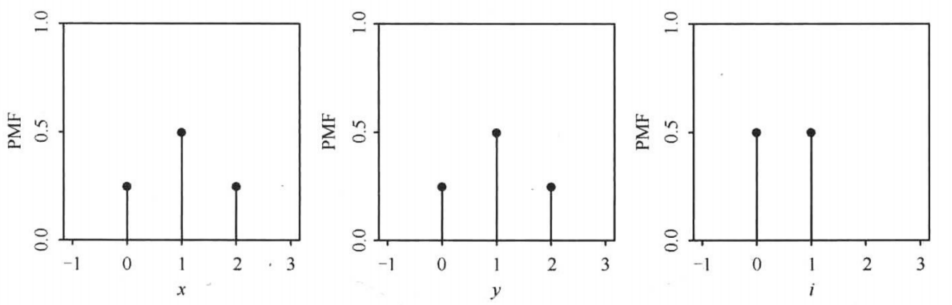
\includegraphics[width=12cm]{figures/Fig3.3.png}
	\end{figure}
\end{frame}

\begin{frame}{}
	\begin{exam}
		掷两颗骰子,其样本空间 $\Omega$ 含有 36 个等可能的样本点
		\begin{eqnarray*}
			\Omega=\{(x,y):x,y=1,2,\cdots,6\}
		\end{eqnarray*}
		令 $X$ 和 $Y$ 表示每个骰子分别出现的点数。试求下面随机变量的分布列: % 在 $\Omega$ 上定义如下三个随机变量,请给出其概率分布列
		\begin{enumerate}[<+-|alert@+>]
			\item $T_1:=X+Y=\mbox{骰子点数之和}$;
			\item $T_2:=14-(X+Y)$;
			\item $T_3:=\mbox{点数为 6 点的骰子的个数}$;
			\item $T_4:=\max\{X, Y\}=\mbox{骰子的最大点数}$
		\end{enumerate}

	\end{exam}
\end{frame}

\begin{frame}
	\begin{itemize}[<+-|alert@+>]
		\item $T_1, T_2$ 的概率分布列为 \pause
		      \begin{eqnarray*}
			      \left(\begin{array}{ccccccccccc}
				      2            & 3            & 4            & 5            & 6            & 7            & 8            & 9            & 10           & 11           & 12           \\
				      \frac{1}{36} & \frac{2}{36} & \frac{3}{36} & \frac{4}{36} & \frac{5}{36} & \frac{6}{36} & \frac{5}{36} & \frac{4}{36} & \frac{3}{36} & \frac{2}{36} & \frac{1}{36}
			      \end{array}\right)
		      \end{eqnarray*}
		      \pause
		      \begin{figure}[图 3.4.png]
			      \centering
			      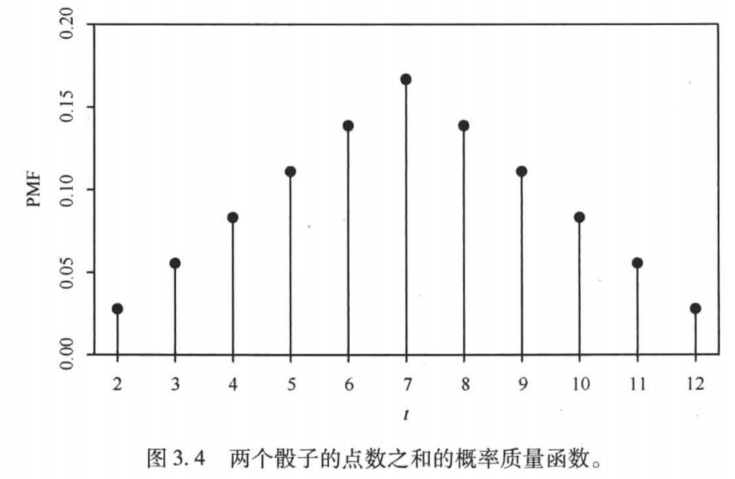
\includegraphics[width=9cm]{figures/Fig3.4.png}
		      \end{figure}

	\end{itemize}

\end{frame}

\begin{frame}
	\begin{itemize}[<+-|alert@+>]

		\item $T_3$ 的概率分布列为 \pause
		      \begin{eqnarray*}
			      \left(\begin{array}{ccc}
				      0             & 1             & 2            \\
				      \frac{25}{36} & \frac{10}{36} & \frac{1}{36}
			      \end{array}\right)
		      \end{eqnarray*}

		\item $T_4$ 的概率分布列为 \pause
		      \begin{eqnarray*}
			      \left(\begin{array}{cccccc}
				      1            & 2            & 3            & 4            & 5            & 6             \\
				      \frac{1}{36} & \frac{3}{36} & \frac{5}{36} & \frac{7}{36} & \frac{9}{36} & \frac{11}{36}
			      \end{array}\right)
		      \end{eqnarray*}
	\end{itemize}

\end{frame}

% \begin{frame}
%   \begin{exam}
%     设离散型随机变量的 $X$ 分布列为
%     \begin{eqnarray*}
%       \left(\begin{array}{ccc}
%               -1  &2 &3\\
%               0.25 & 0.5 & 0.25
%             \end{array}\right)
%     \end{eqnarray*}
%     试求 $P (X\le 0.5), P (1.5<X\le 2.5)$, 并写出 $X$ 的分布函数.
%   \end{exam}

%   \jieda $$P(X\le 0.5)=P(X=-1)=0.25,$$ $$P(1.5<X\le 2.5)=P(X=2)=0.5.$$

%   其分布函数为 \pause
%   \begin{eqnarray*}
%     F(x)=\left\{
%     \begin{array}{ll}
%       \pause  0, &  x<-1\\  \pause
%       \pause 0.25,& -1\le x<2\\  \pause
%       \pause  0.25+0.5=0.75,&  2\le x<3\\  \pause
%       \pause  0.25+0.5+0.25, & x\ge 3 \pause
%     \end{array}\right.
%   \end{eqnarray*}

% \end{frame}


%\subsection{连续型分布}

\begin{frame}
	\frametitle{连续型随机变量及分布}
	\begin{defi}[连续型随机变量] 设 $X$ 为一随机变量,$F (x)$ 为随机变量 $X$ 的分布函数,如果存在非负可积函数 $p (x)$ 使得
		\begin{eqnarray}\label{eq:contrvdist}
			F(x)=\int_{-\infty}^xp(y)dy
		\end{eqnarray}
		则称 $X$ 为连续型随机变量,其分布函数称之为连续型分布函数,函数 $p (x)$ 称为 $X$ 的概率密度函数,简称密度函数或密度.
	\end{defi}
	\pause
	\begin{rmk}
		\begin{itemize}[<+-|alert@+>]
			\item 能够表为 \eqref{eq:contrvdist} 式变上限积分的函数 $F (x)$ 在分析中称为绝对连续函数。绝对连续函数必为连续函数.
			\item 在若干个点上或零测集上改变密度函数 $p (x)$ 的值并不影响其积分的值,从而不影响分布函数 $F (x)$ 的值,这意味着连续分布的密度函数不唯一.
		\end{itemize}
	\end{rmk}

\end{frame}

\begin{frame}
	\frametitle{密度函数的性质}
	容易验证,随机变量 $X$ 的密度函数有以下性质
	\begin{enumerate}[<+-|alert@+>]
		\item 非负性:$p (x)\ge 0$;
		\item 正则性:$\int_{-\infty}^\infty p (x) dx=1$.
	\end{enumerate}

\end{frame}


\begin{frame}
	\frametitle{连续型随机变量分布的一些常见性质}
	\begin{itemize}
		\item $p(x)=F^\prime (x)$;
		\item $P(a< X\le b)=F(b)-F(a)=\int_a^bp(x)dx$;
		\item $0\le P (X=a)\le P (X\in (a-\epsilon,a))=\int_{a-\epsilon}^ap (x) dx\stackrel{\epsilon\rightarrow 0}{\longrightarrow} 0$, 故 $P (X=a)=0$,即连续型随机变量取值单点的概率为 0;
		\item $P(a<X\le b)=P(a\le X<b)=P(a\le X\le b)=P(a<X<b)$;
		\item 对任意的 Borel 集 $B$,
		      \begin{eqnarray*}
			      P(X\in B)=\int_Bp(x)dx
		      \end{eqnarray*}
		\item $P(X\in[x,x+\Delta x])=\int_x^{x+\Delta x}p(y)dy=p(\xi)\Delta x\approx p(x)\Delta x$
	\end{itemize}
\end{frame}
% \begin{frame}
%   \begin{exam}
%     向区间 $(0,a)$ 上任意投点,用 $X$ 表示这个点的坐标。设该点落在 $(0,a)$ 中任一小区间的概率与这个小区间的长度成正比,而与小区间的位置无关。求 $X$ 的分布函数及密度函数.
%   \end{exam}

%   \pause
%   \jieda 记 $X$ 的分布函数为 $F (x)$, 则
%   \begin{itemize}[<+-|alert@+>]
%   \item 当 $x<0$ 时,$\{X\le x\}$ 为不可能事件,故 $F (x)=P (X\le x)=0$;
%   \item 当 $x\ge a$ 时,$\{X\le x\}$ 是必然事件,故 $F (x)=P (X\le x)=1$;
%   \item 当 $x\in [0,a)$ 时, 有 $F (x)=P (X\le x)=P (0\le X\le x)=kx$, 其中 $k$ 为比例系数.
%   \item 注意到 $1=F (a)=P (0\le X\le a)=ka$, 故 $k=1/a$
%   \end{itemize}
%   \pause
%   故 $X$ 的分布函数为
%   \pause
%   \begin{eqnarray*}
%     F(x)=\left\{
%     \begin{array}{ll}
%       0,& x<0\\
%       x/a, & 0\le x<a\\
%       1,& x\ge a
%     \end{array}
%           \right.
%   \end{eqnarray*}
% \end{frame}
% \begin{frame}
%   下面我们求 $X$ 的密度函数,
%   \begin{itemize}
%   \item 当 $x<0$ 或 $x>a$ 时, $p (x)=F^\prime (x)=0$;
%   \item 当 $0<x<a$ 时,$p (x)=F^\prime (x)=1/a$;
%   \item 当 $x=0,a$ 时,$p (x)$ 可取任意值,一般就近取值为宜,不会影响概率的计算.
%   \end{itemize}
%   故 $X$ 的密度函数为
%   \begin{eqnarray*}
%     p(x)=\left\{
%     \begin{array}{ll}
%       1/a,&0<x<a,\\
%       0,&\mbox{其他}.
%     \end{array}
%           \right.
%   \end{eqnarray*}
%   其密度函数也可取为
%   \begin{eqnarray*}
%     p(x)=\left\{
%     \begin{array}{ll}
%       1/a,&0\le x\le a,\\
%       0,&\mbox{其他}.
%     \end{array}
%           \right.
%   \end{eqnarray*}

% \end{frame}

% \begin{frame}
%   \begin{exam}
%     某种型号电子元件的寿命 $X$(以小时计) 具有以下概率密度函数
%     \begin{eqnarray*}
%       p(x)=\left\{
%       \begin{array}{ll}
%         k/x^2,&x>1000,\\
%         0,&\mbox{其他}.
%       \end{array}
%             \right.
%     \end{eqnarray*}
%     其中 $k$ 为未知常数。现有一大批此种元件 (设各元件工作相互独立),问
%     \begin{enumerate}
%     \item 任取 1 只,其寿命大于 1500 小时的概率是多少?
%     \item 任取 4 只,4 只寿命都大于 1500 小时的概率是多少?
%     \item 任取 4 只,至少有一只寿命大于 1500 小时的概率是多少?
%     \item 若已知一只元件寿命大于 1500 小时,则该元件寿命大于 2000 小时的概率是多少?
%     \end{enumerate}

%   \end{exam}
% \end{frame}
%\subsection{其他类型分布}

\begin{frame}{一个连续型随机变量的例子}
\begin{exam}
  考虑概率空间$(\Omega,\mathcal{F}, P)$, 其中$\Omega:=[0,1], \mathcal{F}:=\mathcal{B}([0,1])$, $P(A):=m(A)$即$A$的Lebesgue测度. 定义
  \[\theta(\omega)=\omega, \ \forall \omega\in [0,1].\]
  \pause 显然, $\theta(\omega)$是随机变量, 且其分布函数为\pause
  \begin{eqnarray*}
	F(x)=P(\theta(\omega)\leq x)=\left\{
		\begin{array}{ll}
		 0, & x<0,\\
		 x, & 0\leq x<1\\
		 1, & x\geq 1.
		\end{array}
		\right.
  \end{eqnarray*}
其分布密度为
\[p(x)=F'(x)=1, x\in (0,1).\]

\end{exam}


\end{frame}







\begin{frame}
	\begin{exam}
		定义函数 $F (x)$ 如下
		\begin{eqnarray*}
			F(x)=\left\{
			\begin{array}{ll}
				0,              & x< 0,      \\
				\dfrac{1+x}{2}, & 0\le x< 1, \\
				1,              & x\ge 1.
			\end{array}
			\right.
		\end{eqnarray*}
		试说明  \begin{enumerate}
			\item $F (x)$ 为分布函数;
			\item $F (x)$ 既非离散型也非连续型分布;
			\item $F (x)$ 可分解为
			      \begin{eqnarray*}
				      F(x)=\frac{1}{2}F_1(x)+\frac{1}{2}F_2(x)
			      \end{eqnarray*}
			      \pause  其中 \begin{eqnarray*}
				      F_1(x)=\left\{
				      \begin{array}{ll}
					      0, & x< 0,    \\
					      1, & x\ge 0.
				      \end{array}
				      \right.
				      \quad  F_2(x)=\left\{\begin{array}{ll}
					      0, & x<0,       \\
					      x, & 0\le x< 1, \\
					      1, & x\ge 1.
				      \end{array}
				      \right.
			      \end{eqnarray*}
		\end{enumerate}

	\end{exam}
\end{frame}


\begin{frame}
	\frametitle{勒贝格分解}
	\begin{thm}[勒贝格分解] 对任一分布函数 $F (x)$ 有如下分解
		\begin{eqnarray*}
			F(x)=c_1F_1(x)+c_2F_2(x)+c_3F_3(x),
		\end{eqnarray*}
		其中常数 $c_1,c_2,c_3\ge 0, c_1+c_2+c_3=1,$ 而 $F_1 (x),F_2 (x),F_3 (x)$ 都是分布函数,$F_1 (x)$ 为纯跳跃离散型函数,$F_2 (x)$ 为连续型分布函数,$F_3 (x)$ 为奇异型分布函数(见教材3.6节奇异连续型分布构造).
	\end{thm}
	\vspace{0.3cm}
	\pause
	\begin{itemize}[<+-|alert@+>]
		\item 上述定理中奇异函数的含义及定理的证明可参见一般的实变函数论教科书,这里我们不再详述,仅指出几种特殊情况:
		      \begin{itemize}
			      \item 在分解式中取 $c_1=1,c_2=c_3=0$ 便得到我们所讨论的离散型分布函数;
			      \item 在分解式中取 $c_2=1,c_1=c_3=0$ 便得到连续型分布函数;
			      \item 若取 $c_3=0, c_1\neq 0, c_2\neq 0, c_1+c_2=1$ 便得到离散与连续混合分布
		      \end{itemize}
		\item 从上面分析可看出,随机变量除了离散型与连续型外还有很多其他类型.
	\end{itemize}

\end{frame}


\subsection{随机变量的存在性}

 \begin{frame}{分布函数与随机变量}
 \begin{align*}
 &	\left. \begin{array}{c}
		 (\Omega, \mathcal{F}, P) \\
		  \\
		 X(\omega)
			\end{array}\right\}\Rightarrow\pause P(X\leq x)=: F(x)\pause	\Rightarrow  \left\{\begin{array}{l}
		   \mbox{单调非降性} \\
		   \mbox{右连续性}\\
		   \mbox{规范性}
		\end{array}\right. \\
 \pause
 \\
 \\
 &\left.\begin{array}{r}
	 \mbox{单调非降性} \\
	 \mbox{右连续性}\\
	 \mbox{规范性}
 \end{array}\right\}\mbox{的} F (x) \mbox{给定}\Rightarrow\pause \mbox{存在}  \left\{\begin{array}{l}
		 (\Omega, \mathcal{F}, P) \\
		 \\
		 X(\omega)
	 \end{array}\right. \mbox{使得} F (x)=P (X\leq x) ?
 \end{align*}


 \end{frame}

 \begin{frame}{随机变量的存在性问题分析}
 %	由前面所学知识易知:给定一个随机变量,我们可定义其分布函数,并且分布函数具有性质:单调非降,右连续,$F (-\infty)=0$, $F (+\infty)=1$. 那么反过来呢?
 %	\pause \begin{prob}
 %		给定一个分布函数 $F (x)$, 即函数 $F (x)$ 具有分布函数的性质:单调非降,右连续,$F (-\infty)=0$, $F (+\infty)=1$, 是否一定存在一个概率空间 $(\Omega,\mathcal{F},P)$ 及其上的随机变量 $X$ 使得其分布函数恰为 $F (x)$?
 %	\end{prob}
 %	\pause
 \begin{thm}\label{sec:existofrv}
 \hspace{-0.2cm} 若 $F (x)$ 是右连续、单调非降函数,且 $F (-\infty)=0, F (+\infty)=1$, 则存在一个概率空间 $(\Omega,\mathcal{F},P)$ 及其上的随机变量 $X (\omega)$, 使 $X (\omega)$ 的分布函数恰好是 $F (x)$.
 \end{thm}

 \textcolor{cyan}{分析:}
 \begin{itemize}[<+-|alert@+>]
	 %\item 取 $\Omega=[0,1]$, $\mathcal{F}$ 为 $[0,1]$ 上的 Borel 集全体,取 $P$ 为直线上的 Lebesgue 测度 (是长度概念的推广,但对一切 Borel 集有定义);
	 \item 对 $[0,1]$ 上的均匀分布随机变量 $\theta (\omega)=\omega$, 其分布函数为 % 有 %, 其分布函数 % 则 $\theta (\omega)$ 是 $(\Omega,\mathcal{F},P)$ 上的随机变量,并且,,
	 \begin{eqnarray*}
		 P(\theta(\omega)\le x)=P(\omega\in[0,x])=x, \ \forall x\in[0,1];
	 \end{eqnarray*}
	 \item $F (x)\in[0.1]$, 若将上式中的 $x$ 替换为 $F (x)$, 则有
		 \begin{eqnarray*}
		 P(\theta(\omega)\le F(x))=F(x);
	 \end{eqnarray*}
	 \item 若分布函数 $F (x)$ 可逆,则
	 \begin{eqnarray*}
	 P(F^{-1}(\theta(\omega))\le x)=	P(\theta(\omega)\le F(x))=\pause F(x);
	 \end{eqnarray*}

	 \item 考虑 $X (\omega):=F^{-1}(\theta (\omega))$, 则 $F_X (x)= P (F^{-1}(\theta (\omega))\le x)= F (x)$;

 %    \item $F (x)$\textcolor{red}{不一定可逆}, 能否定义一种映射 $G$ 使得
 %    \[\{\theta(\omega)\le F(x)\}=\{G(\theta(\omega))\le x\}?\]

 \end{itemize}


 \end{frame}
 \begin{frame}{随机变量的存在性问题分析}
	 \begin{itemize}[<+-|alert@+>]
	 \item $F (x)$\textcolor{red}{不一定可逆}, 能否定义一个函数 $G$ 使得
		 \[\{\theta(\omega)\le F(x)\}=\{G(\theta(\omega))\le x\}?\]
	 \item 上述等式也即寻求如下等价性
	 \[G(\theta)\leq x \Leftrightarrow F(x)\ge \theta \]
	 \item 因此,若函数 $G$ 存在,则对任意给定的 $\theta$ 必须满足
	 \[G(\theta)\leq x, \quad  \forall x\in \{x: F(x)\ge\theta\}\]
	 \item 故所寻找的函数 $G$ 需有以下性质
	 \[G(\theta)\leq \inf\{x:F(x)\geq \theta\}\]
	 \item 上述不等式右侧的下确界也是 $G$ 的一种选择,可以证明选此下确界作为函数 $G$ 的定义的确具有我们所要求的性质.%,
	 \end{itemize}




 \end{frame}

 \begin{frame}{单调逆 (一般逆) 的定义}
	 \vspace{-0.1cm}
	 \begin{defi}
		 设 $F (x)$ 是右连续、单调非降函数,且 $F (-\infty)=0, F (+\infty)=1$. 对任意的 $p\in (0,1)$, 我们称
		 \begin{eqnarray*}
			 F^{-1}(p):=\inf\{x: F(x)\geq p\}, %\forall p\in (0,1),
		 \end{eqnarray*}
		 为函数 $F (x)$ 的单调逆或一般逆.
	 \end{defi}

 \pause
 \begin{rmk} \ 	 $F^{-1}(p)$ 在概率论中也称为函数 $F (x)$ 的 $p$ 分位数函数或与其相对应的随机变量 $X$ 的 $p$ 分位数,通常用 $x_p$ 或 $\xi_p$ 来表示.
 \end{rmk}
 \begin{thm}
	 设 $F (x), F^{-1}(p)$ 定义如上,则
	 \[F^{-1}(p)\leq x \Leftrightarrow F(x)\ge p \]
 \end{thm}
 \pause
 \zheng 令 $A:=\{y: F (y)\geq p\}$, 则 \pause
 \begin{itemize}[<+-|alert@+>]
	 \item $\Leftarrow$: $F (x)\geq p$ 蕴含 \pause $F^{-1}(p):=\inf A\leq x$\pause
	 \item $\Rightarrow$: $F^{-1}(p)\leq x$ 即 $x\geq F^{-1}(p):=\inf A=:x_0$\pause
	 \begin{itemize}[<+-|alert@+>]
		 \item 若 $x_0\in A$, 则显然 \pause $F (x)\geq F (x_0)\geq p$\pause
		 \item 若 $x_0\notin A$, 则存在 \pause $\{x_n\}_{n\geq 1}\subset A$ 使得 $x_n>x_0$ 且 $\lim_{n\rightarrow \infty} x_n=x_0$,\pause  从而 \pause
		 \[F(x)\geq F(x_0)=F(\lim_{n\rightarrow \infty}x_n)=\pause \lim_{n\rightarrow \infty}F(x_n)\geq\pause p;\]
	 \end{itemize}
 \end{itemize}
 \end{frame}
 \begin{frame}{随机变量存在性的证明}
 \trc{定理 \ref{sec:existofrv} 的证明:}\pause
 \begin{itemize}[<+-|alert@+>]
	 \item 取 $\Omega=[0,1]$, $\mathcal{F}$ 为 $[0,1]$ 上的 Borel 集全体,取 $P$ 为直线上的 Lebesgue 测度 (是长度概念的推广,但对一切 Borel 集有定义);
	 \item 定义: $\theta (\omega)=\omega$, 则 $\theta (\omega)$ 是 $(\Omega,\mathcal{F},P)$ 上的随机变量,并且,对一切的 $0\le x\le 1$,
	 \begin{eqnarray*}
		 P(\theta(\omega)\le x)=P(\omega\in[0,x])=x;
	 \end{eqnarray*}
	 \item 考虑 $X (\omega):=F^{-1}(\theta (\omega))$, 则
	{\small\begin{eqnarray*}
			 F_X(x)=P(X\le x)=\pause P(F^{-1}(\theta(\omega))\le x)\pause \xlongequal[p\le F(x)]{F^{-1}(p)\le x} P(\theta(\omega)\le F(x))=\pause F(x)
	 \end{eqnarray*}}


 \end{itemize}


 \end{frame}



 %\begin{frame}
 %	\frametitle{随机变量的 $p$ 分位数函数}
 %	\vspace{-0.3cm}
 %	\begin{defi}
 %		设 $X$ 是概率空间 $(\Omega,\mathcal{F},P)$ 上的随机变量,$F (x)$ 为其分布函数。对于 $p\in (0,1)$, 定义
 %		\begin{eqnarray*}
 %			F^{-1}(p):=\sup\{x:F(x)<p\}\pause =\inf\{x: F(x)\geq p\}.
 %		\end{eqnarray*}
 %		称 $F^{-1}(p)$ 为 $F$ 或 $X$ 的 $p$ 分位数,通常用 $x_p$ 或 $\xi_p$ 来表示.
 %	\end{defi}
 %
 %
 %\end{frame}
 \begin{frame}
	 \frametitle{单调逆 (一般逆) 的性质}

	 \begin{itemize}[<+-|alert@+>]
		 \item $F^{-1}(F (x))\leq x, \forall x\in R$ :\pause\  设 $x_0\in R$ 任意给定且 $F (x_0)=p_0$, 则 \pause
		 \begin{align*}
		  F^{-1}(F(x_0))&=\pause F^{-1}(p_0)=\pause \inf\{x: F(x)\geq p_0\}\\
		  &=\pause \inf\{x: F(x)\geq F(x_0)\}\leq\pause  x_0
		 \end{align*}
		 \item $F (F^{-1}(p))\geq p, \forall p\in (0,1)$:\pause 设 $p_0\in (0,1)$ 任意给定且
		 \begin{align*}
		 F^{-1}(p_0)=x_0=\inf\{x: F(x)\geq p_0\}=:\inf A, %
		 \end{align*}
	 \begin{itemize}[<+-|alert@+>]
		 \item 若 $x_0\in A$, 则显然有 $F (F^{-1}(p_0))=F (x_0)\geq p_0$;
		 \item 若 $x_0\notin A$, 则 \pause 存在 $\{x_n\}_{n\geq 1}\subset A$ 使得 $x_n>x_0$ 且 $\lim_{n\rightarrow \infty} x_n=x_0$,\pause  从而由函数 $F (x)$ 的右连续性可知 \pause
		 \[F(F^{-1}(p_0))=F(x_0)=F(\lim_{n\rightarrow \infty}x_n)=\pause \lim_{n\rightarrow \infty}F(x_n)\geq\pause p_0;\]
	 \end{itemize}
	 \item $F^{-1}(p)$ 关于 $p$ 单调非降:集合 $\{x:F (x)\geq p\}$ 关于 $p$ 单调不增,故其下确界也关于 $p$ 单调非降
		 \end{itemize}
	 \end{frame}

 \begin{frame}
	 \frametitle{单调逆 (一般逆) 的性质}
	 下面的几条性质 %,\trc{(留做作业)}
	 \begin{itemize}[<+-|alert@+>]
		 \item  $F^{-1}(p)$ 关于 $p$ 是左连续的;
		 \item $F^{-1}(p):=\inf\{x: F(x)\geq p\}=\sup\{x:F(x)<p\}$
		 \item $x<F^{-1}(p)\Leftrightarrow F(x)<p$
		 %\item $F (x)<p$, 则 $x<F^{-1}(p)$
	 \end{itemize}

 \end{frame}

 \begin{frame}{思考}
	 若 $F (x)$ 是左连续、单调非降函数,且 $F (-\infty)=0, F (+\infty)=1$, 是否存在一个概率空间 $(\Omega,\mathcal{F},P)$ 及其上的随机变量 $X (\omega)$, 使得
	 \[F(x)=P(X<x).\]



 \end{frame}


 \title[概率论]{第十一讲:常见的离散型随机变量}
\institute[东南大学数学学院]{\large \textrm{Email: xzhangseu@seu.edu.cn} \\ \quad  \\
	\large 东南大学 \quad 数学学院 \\
	\vspace{0.3cm}
	%  \trc{公共邮箱: \textrm{zy.prob@qq.com}\\
	%    \hspace{-1.7cm}  密 \qquad 码: \textrm{seu!prob}}
}
\date{}


{\setbeamertemplate{footline}{}
	\begin{frame}
		\titlepage
	\end{frame}
}
% \begin{CJK*}{GBK}{song}

%   \title{简单随机抽样}
%   \author{林语堂}
%   \institute{University}
%   \date{2009-03-31}
%   \date{}
%   \begin{frame}
%     \titlepage
%   \end{frame}

%   \begin{frame}
%     \frametitle{第二章:简单随机抽样}
%     \tableofcontents
%   %     You might wish to add the option[pausesections]
%   \end{frame}

%   \AtBeginSubsection[]{
%   \begin{frame}<beamer>
%     \frametitle{Outline}
%     \tableofcontents[currentsection,currentsubsection]
%   \end{frame}
% }
%   定义目录页



% \begin{frame}[plain]
%   \frametitle{目录}
%   \setcounter{tocdepth}{2}
%   \tableofcontents
% \end{frame}
\addtocounter{framenumber}{-3}  % 目录页不计算页码
%\section{随机变量}
\subsection{伯努利试验及其离散型分布}
\begin{frame}
	\frametitle{伯努利实验}
	\begin{itemize}[<+-|alert@+>]
		\item 只有两种可能结果的试验称为伯努利试验;例如抽检产品,可能是合格品,也可能是次品;掷两颗骰子,可能得到同点,也可能得到不同点,等等都是伯努利试验.
		\item 伯努利试验的样本空间 $\Omega$ 并不一定只含有两个样本点,有时只是把我们所关心的一部分样本点归结为一种结果 $A$, 同时把其余的样本点的集合看作另一种结果 $\bar{A}$;
		\item 在上述掷骰子的试验中,样本空间 $\Omega$ 共含有 36 个样本点,如果我们只关心同点是否发生,就可以把其中的 6 个样本点组成的事件 $A:=\{(i,i):i=1,\cdots, 6\}$ 视为一种结果,而其余的 30 个样本点组成另一结果 $\bar{A}:=\{\mbox{不同点}\}$;
		\item 此外我们不再关心由 $\Omega$ 的其他非空子集组成的事件,于是对于伯努利试验而言,事件 $\sigma$ 代数应取为 $\mathcal{F}=\{\emptyset, A, \bar{A}, \Omega\}$;
		\item 通常把结果 $A$ 称作 "成功", 而把 $\bar{A}$ 称作 "失败";
		\item 再取定成功失败的概率 $p=P (A), q=P (\bar{A})$ ($p>0,q>0$ 且 $p+q=1$), 则建立了一次伯努利试验的概率空间 $(\Omega,\mathcal{F},P)$.
	\end{itemize}
\end{frame}
\begin{frame}
	\begin{itemize}[<+-|alert@+>]
		\item 在概率论的理论与应用中,经常以一系列独立重复的伯努利试验作为概率模型;
		\item 所谓重复,粗略的说即各次试验的概率空间都是上述的 $(\Omega,\mathcal{F},P)$;
		\item 而 $n$ 个试验的独立性则是指各次试验的结果互不影响,即对于第 $i$ 次试验的任何结果 $E_i (i=1,\cdots, n)$ 均有
		      \begin{eqnarray*}
			      P(E_1E_2\cdots E_n)=P(E_1)P(E_2)\cdots P(E_n)
		      \end{eqnarray*}
		\item 将一次伯努利试验独立重复 $n$ 次,称作 $n$ 重伯努利试验;
		\item 将一次伯努利试验独立地重复下去所得到的一系列试验,称为可列重伯努利试验.
	\end{itemize}
\end{frame}

\begin{frame}
	\frametitle{二项分布:$n$ 重伯努利试验中成功的次数 $X$}
	\begin{itemize}[<+-|alert@+>]
		\item $X$:$n$ 重伯努利试验中成功 (事件 $A$ 发生) 的次数;
		\item $X$ 的所有可能取值为: $0, 1, \cdots, n$;
		\item 下面我们考虑 $X$ 的分布列
		      \begin{itemize}
			      \item $n$ 重伯努利试验的样本空间: $\Omega:=\{\omega=(\omega_1,\cdots,\omega_n):\omega_i\mbox{或者为} A\mbox{或者为}\bar{A}\}$
			      \item 样本空间样本点的个数为 $2^n$ 个;
			      \item $\{X=k\}=\{\omega=(\omega_1,\cdots,\omega_n):\omega_1,\cdots,\omega_n\mbox{中有} k\mbox{个} A\}$, 共包含 $C_n^k$ 个样本点;
			      \item 若任给样本点 $\omega=(\omega_1,\cdots,\omega_n)\in \{X=k\}$, 则意味着 $\omega_1,\cdots,\omega_n$ 中有 $k$ 个 $A$, $n-k$ 个 $\bar{A}$, 故由独立性可知
			            \begin{eqnarray*}
				            P(\omega)=p^k(1-p)^{n-k}
			            \end{eqnarray*}
			      \item 而事件 $\{X=k\}$ 中共有 $C_n^k$ 个类似的 $\omega$, 故
			            \begin{eqnarray*}
				            P(X=k)=C_n^kp^k(1-p)^{n-k}:=b(k;n,p), k=0,1,\cdots, n
			            \end{eqnarray*}
			            这个分布常称为二项分布,记为 $X\sim B (n,p)$.
			      \item 容易验证,$\sum_{k=0}^nC_n^kp^k (1-p)^{n-k}=(p+1-p)^n=1$
		      \end{itemize}
	\end{itemize}

\end{frame}
\begin{frame}
	\frametitle{两点分布}
	\begin{itemize}
		\item $n=1$ 时的二项分布 $B (1,p)$ 称为二点分布,或 $0-1$ 分布,或称伯努利分布,其分布列为
		      \begin{eqnarray*}
			      P(X=k)=p^k(1-p)^{1-k}, k=0, 1
		      \end{eqnarray*}
		      或记为
		      \begin{eqnarray*}
			      \left(\begin{array}{cc}
				      0,   & 1  \\
				      1-p, & p
			      \end{array}\right)
		      \end{eqnarray*}
		\item $B (1,p)$ 主要用于描述一次伯努利试验中成功的次数 (0 或 1);
		\item 若记 $X_i$ 表示第 $i$ 次伯努利试验中成功的次数,则 $X_i$ 相互独立且有
		      \begin{eqnarray*}
			      X=X_1+X_2+\cdots X_n
		      \end{eqnarray*}
		      即二项分布随机变量可写为 $n$ 个独立同为两点分布随机变量的和.
	\end{itemize}
\end{frame}
\begin{frame}
	\frametitle{二项分布的性质}
	\begin{itemize}[<+-|alert@+>]
		\item 对 $k\ge 1$, 考虑比值
		      \begin{eqnarray*}
			      \dfrac{b(k;n,p)}{b(k-1;n,p)}&=&\pause \dfrac{C_n^kp^k(1-p)^{n-k}}{C_n^{k-1}p^{k-1}(1-p)^{n-k+1}}=\pause \dfrac{(n-k+1)p}{k(1-p)}\\
			      &=&\pause \dfrac{k(1-p)+(n+1)p-k}{k(1-p)}=\pause 1+\dfrac{(n+1)p-k}{k(1-p)}
		      \end{eqnarray*}
		\item 当 $(n+1) p>k$ 时,$b (k;n,p)>b (k-1;n,p)$;
		\item 当 $(n+1) p<k$ 时,$b (k;n,p)<b (k-1;n,p)$;
		\item 从而,对于固定的 $n,p$,$\{X=k\}$ 的概率 $b (k;n,p)$ 先随 $k$ 增大而增大,再随 $k$ 增大而减小,故必有最大值:
		      \begin{itemize}
			      \item 如果 $m:=(n+1) p$ 为整数,则 $b (m;n,p)=b (m-1;n,p)$ 同为 $b (k;n,p)$ 的最大值
			      \item 如果 $(n+1) p$ 不为整数,则 $b (k;n,p)$ 在 $m=[(n+1) p]$ 处取到最大值 (此处 $[a]$ 表示不超过 $a$ 的最大整数)
		      \end{itemize}
		\item 我们称使得 $b (k;n,p)$ 取得最大值的 $m$ 为二项分布随机变量的最可能值,或称为 $n$ 重伯努利试验中最可能的成功次数.
	\end{itemize}
\end{frame}


\begin{frame}{二项分布的性质}
	\begin{thm}\label{338} 设 $X\sim B (n,p)$, 且 $q=1-p$(通常用 $q$ 表示伯努利试验失败的概率), 则有 $n-X\sim B (n,q)$.
	\end{thm}

	\pause
	% \begin{jieda}
	\begin{itemize}[<+-|alert@+>]
		\item 借用二项分布的直观定义:将 $X$ 为 $n$ 次独立伯努利试验成功的次数,则 $n-X$ 为这些试验中失败的次数.
		\item 互相交换成功与失败的角色,可知 $n-X\sim B (n,q)$.
		\item 也可从分布列 (概率质量函数) 的角度出发得到
		      $n-X\sim B(n,q).$
		\item 令 $Y=n-X$, 则 $Y$ 的分布列 (概率质量函数) 为 \pause
		      \begin{equation*}
			      \begin{aligned}
				      P(Y=k)= & P(n-X=k)=P(X=n-k)                                                           \\
				      =       & \left(\begin{matrix}
						                      n   \\
						                      n-k \\
					                      \end{matrix}\right)p^{n-k}q^{k}=\left(\begin{matrix}
						                                                            n \\
						                                                            k \\
					                                                            \end{matrix}\right)q^kp^{n-k},
			      \end{aligned}
		      \end{equation*}
	\end{itemize}
	% \end{jieda}
\end{frame}

\begin{frame}{二项分布的性质}

	\begin{thm} 设 $X\sim B (n,p)$, 其中 $n$ 为偶数,$p=1/2$, 则 $X$ 的分布关于 $n/2$ 对称,即对任意的非负整数 $j$, 均有
		$$P(X=\frac{n}{2}+j)=P(X=\frac{n}{2}-j).$$
	\end{thm}
	\pause
	%\vspace{0.2cm}

	\begin{jieda} 由定理 \ref{338} 可知,$n-X$ 同样服从 $B (n,1/2)$. \pause 因此对任意非负整数 $k$ 均有
		$$P(X=k)=P(n-X=k)=P(X=n-k).$$
		\pause
		令 $k=n/2+j$, 即可得证. % 得推论 \ref{338} 的结果。该推论也解释了为什么图 3.6 中 $Bin (10,1/2)$ 是关于 5 对称的.
	\end{jieda}

	%\begin{exam}({\tc 掷硬币续}) 回顾例 \ref{312}, 现在已经知道 $X\sim Bin (2,1/2),Y~\sim Bin (2,1/2)$ 和 $I\sim Bern (1/2)$. 由定理 \ref{337} 可知,$X$ 和 $Y=2-X$ 具有相同的分布。再根据推论 \ref{338}, 得到 $X$ 的分布 (以及 $Y$ 的分布) 是关于 1 对称的.
	%\end{exam}
\end{frame}






\begin{frame}
	\vspace{0.4cm}
	\begin{exam}
		设每台自动机床在运行过程中需要维修的概率均为 $p=0.01$, 并且各机床是否需要维修相互独立。如果:
		\begin{enumerate}
			\item 每名维修工人负责看管 20 台机床;
			\item 3 名维修工人负责看管 80 台机床;
		\end{enumerate}
		求机床不能及维修的概率.
	\end{exam}

	\pause \jieda 1. 这是 $n=20$ 重伯努利试验,参数 $p=0.01$, 故需要维修的机床数 $X$ 服从 $B (20,0.01)$ 分布。故不能及时维修的概率为 \pause
	\begin{eqnarray*}
		P(X>1)&=&\pause 1-P(X\le 1)=\pause 1-P(X=0)-P(X=1)\\
		&=&\pause 1-C_{20}^00.01^0(1-0.01)^{20}-C_{20}^10.01(1-0.01)^{20-1}\approx 0.0169
	\end{eqnarray*}
	\pause 2. 此时需要维修的机床数 $X$ 服从 $B (80,0.01)$ 分布,类似可得不能及时维修的概率为
	\begin{eqnarray*}
		P(X>3)=1-\sum_{k=0}^3b(k;80,0.01)\approx 0.0087
	\end{eqnarray*}

\end{frame}

\begin{frame}
	\frametitle{小概率事件终将发生}
	\begin{exam}
		在可列重伯努利试验中,求事件 $E:=\{\mbox{试验终将成功}\}$ 的概率.
	\end{exam}
	\pause

	\jieda 考虑所求概率事件的反面即 $\overline{E}:=\{\mbox{试验永不成功}\}$.\pause 若我们记
	\begin{eqnarray*}
		F_n:=\{\mbox{前} n\mbox{次试验均失败}\},
	\end{eqnarray*}
	\pause
	则易知,$\{F_n\}$ 为单调下降事件序列,且
	\begin{eqnarray*}
		\lim_{n\rightarrow \infty}F_n=\pause \cap_{n=1}^\infty F_n=\pause \overline{E}
	\end{eqnarray*}
	\pause 从而
	\begin{eqnarray*}
		P(\overline{E})=\pause P(\lim_{n\rightarrow\infty}F_n)=\pause \lim_{n\rightarrow\infty }P(F_n)=\pause \lim_{n\rightarrow\infty }C_n^0p^0(1-p)^n=\pause 0
	\end{eqnarray*}
	\pause 故
	\begin{eqnarray*}
		P(E)=1-P(\overline{E})=1-0=1
	\end{eqnarray*}
	\pause 无论成功的概率有多小,但是试验最终成功的概率为 1, 也就是说小概率事件终将发生的概率为 1.
\end{frame}

%   \title[概率论]{第十一讲:常见的离散型随机变量 (II)}
%   \author[张鑫 {\rm Email: x.zhang.seu@foxmail.com} ]{\large 张 鑫}
%   \institute[东南大学数学学院]{\large \textrm{Email: x.zhang.seu@foxmail.com} \\ \quad  \\
%   	\large 东南大学 \quad 数学学院 \\
%   	\vspace{0.3cm}
%   	%  \trc{公共邮箱: \textrm{zy.prob@qq.com}\\
%   		%    \hspace{-1.7cm}  密 \qquad 码: \textrm{seu!prob}}
%   }
%   \date{}



%   	{ \setbeamertemplate{footline}{}
%   		\begin{frame}
%   			\titlepage
%   		\end{frame}
%   	}

%   	% \begin{frame}[plain]
%   		%   \frametitle{目录}
%   		%   \setcounter{tocdepth}{2}
%   		%   \tableofcontents
%   		% \end{frame}
%   	\addtocounter{framenumber}{-3}  % 目录页不计算页码
%   	\section{随机变量}
%   	\subsection{伯努利试验及其离散型分布}

\begin{frame}
	\frametitle{几何分布:可列重伯努利试验中首次成功的等待时间 $X$}
	\begin{itemize}[<+-|alert@+>]
		\item 记 $X$ 为可列重伯努利试验中首次成功的等待时间即首次成功所需要试验的次数;
		\item $\{X=k\}=\{\underbrace{\overline{A}\cdots \overline{A}}_{k-1\mbox{个}} A\}$, 故
		      \begin{eqnarray*}
			      P(X=k)=(1-p)^{k-1}p:=g(k;p), k=1,\cdots,
		      \end{eqnarray*}
		      这个分布常称为几何分布,记为 $X\sim G (p)$.
	\end{itemize}
\end{frame}
\begin{frame}
	\frametitle{几何分布的性质}
	\begin{thm}
		取值自然数的随机变量 $X$ 为几何分布当且仅当 $X$ 有无记忆性:
		\begin{eqnarray}\label{eq:memory}
			P (X>m+n|X>m)=P (X>n), \mbox{对任意的} m,n \ge 1.
		\end{eqnarray}
	\end{thm}
	\zheng 若 $X$ 为几何分布,则
	\begin{eqnarray*}
		P(X>m+n|X>m)=\pause \dfrac{P(X>m+n,X>m)}{P(X>m)}=\pause \dfrac{P(X>m+n)}{P(X>m)}
	\end{eqnarray*}
	\pause 而
	\begin{eqnarray*}
		P(X>n)=\pause \sum_{k=n+1}^\infty (1-p)^{k-1}p=\pause \dfrac{(1-p)^{n}p}{1-(1-p)}=\pause (1-p)^n
	\end{eqnarray*}
	\pause 故
	\begin{eqnarray*}
		P(X>m+n|X>m)=\dfrac{(1-p)^{m+n}}{(1-p)^m}=(1-p)^n=P(X>n)
	\end{eqnarray*}

\end{frame}

\begin{frame}
	\vspace{0.5cm}
	若 $X$ 具有无记忆性,则由~\eqref{eq:memory} 知
	\pause \begin{eqnarray*}
		Q_n:=P (X>n)>0, \quad \mbox{对任意的} n\ge 1
	\end{eqnarray*}
	\pause 并且有
	\begin{eqnarray*}
		Q_{m+n}=P(X>m+n)=\pause P(X>m)P(X>m+n|X>m)=\pause Q_mQ_n
	\end{eqnarray*}
	\pause 从而 \vspace{-0.7cm}
	\begin{eqnarray*}
		Q_m=Q_1^m
	\end{eqnarray*}
	\pause 注意到 $Q_1\in (0,1)$, 事实上,
	\begin{itemize}[<+-|alert@+>]
		\item $Q_1=P (X>1)>0$ 显然;
		\item  若 $Q_1=1$, 则对一切的 $m$ 均有 $Q_m=P (X>m)=1$, 这与 $X$ 取自然数矛盾,故 $Q_1\in (0,1)$.
	\end{itemize}
	\pause 故取 $p=1-Q_1\in (0,1)$, 且对任意的 $k\ge 1$ 有
	\begin{eqnarray*}
		P(X=k)&=&\pause P(X>k-1)-P(X>k)=\pause Q_{k-1}-Q_k\\
		&=&\pause (1-p)^{k-1}-(1-p)^k=\pause (1-p)^{k-1}p
	\end{eqnarray*}

\end{frame}

\begin{frame}
	\frametitle{无记忆性}
	\begin{eqnarray*}
		P(X>m+n|X>m)=P(X>n)
	\end{eqnarray*}
	\begin{itemize}[<+-|alert@+>]
		\item 上述的无记忆性表明:已知试验了 $m$ 次未获得成功,再加做 $n$ 次试验仍不成功的概率,等于从开始算起做 $n$ 次试验都不成成功的概率.
		\item 换句话放,已做过的 $m$ 次失败的试验被忘记了;
		\item 产生几何分布的这种无记忆性的根本原因在于,我们进行的是独立重复试验,这是不学习,不总结经验的试验,已经做过的试验当然不会留下记忆.
	\end{itemize}
\end{frame}

\begin{frame}
	\vspace{0.3cm}
	\begin{exam}
		10 把外形相同的钥匙中只有一把能打开门。现一一试开,试对每次试毕放回与不放回两种情形,分别求事件 $E:=\{\mbox{至多试} 3\mbox{次能打开门}\}$ 的概率.
	\end{exam}

	\pause
	\jieda 1. 放回情形是独立重复试验,属伯努利概型。以 $X$ 表示首次打开门的等待时间,则 $X$ 服从几何分布 $G (0.1)$. 故所求概率为
	\begin{eqnarray*}
		P(E)=P(X\le 3)=\sum_{k=1}^3(1-0.1)^{k-1}0.1=0.271
	\end{eqnarray*}
	\pause
	2. 不放回情形不再是独立重复试验,适用于古典概型。样本点总数 $n (\Omega)=C_{10}^3$, 而 $n (\overline{E})=C_9^3$. 故
	\begin{eqnarray*}
		P(E)=1-P(\overline{E})=1-\dfrac{C_9^3}{C_{10}^3}=0.3
	\end{eqnarray*}
	\pause 或令 $A_i:=\{\mbox{第} i\mbox{次取到能开门的钥匙}\}$, 则 $A_1,A_2,A_3$ 互不相容,由可加性及抽签的公平性可得
	\begin{eqnarray*}
		P(E)=P(\cup_{i=1}^3A_i)=\sum_{i=1}^3P(A_i)=0.3
	\end{eqnarray*}

\end{frame}
\begin{frame}
	\frametitle{帕斯卡 (Pascal) 分布:第 $r$ 次成功的等待时间}
	\begin{itemize}[<+-|alert@+>]
		\item 记 $X_r$ 为可列重伯努利试验中第 $r$ 次成功的等待时间即第 $r$ 次成功所需要试验的次数;
		\item 易见 $X$ 的所有可能取值为 $k=r, r+1,\cdots, $ 并且有
		      \begin{eqnarray*}
			      \{X_r=k\}&=&\{\mbox{前} k-1\mbox{次试验恰有} r-1\mbox{次成功且第} k\mbox{次成功}\}\\
			      \pause
			      P (X_r=k)&=&\pause P (\mbox{前} k-1\mbox{次试验恰有} r-1\mbox{次成功}) P (\mbox{第} k\mbox{次成功})\\
			      &=&\pause C_{k-1}^{r-1}p^{r-1}(1-p)^{k-1-(r-1)}p\\
			      &=&\pause C_{k-1}^{r-1}p^r(1-p)^{k-r}:=f(k;r,p), \quad k=r, r+1,\cdots
		      \end{eqnarray*}
		      \pause 这个分布常称为帕斯卡 (Pascal) 分布或负二项分布.
		\item $f (k;r,p), k=r,r+1,\cdots,$ 可以成为离散型分布的密度,事实上: $f (k;r,p)>0$ 显然,其和
		     {\small \begin{eqnarray*}
			      \sum_{k=r}^\infty f(k;r,p)&=&\pause  \sum_{k=r}^\infty C_{k-1}^{r-1}p^r(1-p)^{k-r}\xlongequal[q=1-p]{k-r=i}\pause \sum_{i=0}^\infty C_{r+i-1}^{r-1}p^rq^{r+i-r}\\
			      &=&\pause \sum_{i=0}^\infty C_{r+i-1}^ip^rq^i=\pause \sum_{i=0}^\infty C_{-r}^ip^r(-q)^i=\pause p^r(1-q)^{-r}=1 \end{eqnarray*}
		      }
	\end{itemize}
\end{frame}
\begin{frame}
	\frametitle{帕斯卡分布的性质}
	\begin{itemize}[<+-|alert@+>]
		\item 若帕斯卡分布中的 $r=1$, 则此时的帕斯卡分布即为几何分布;
		\item 如果记 $$\tau_1=X_1, \quad \tau_n=X_n-X_{n-1}, \quad n>1, $$ 则随机变量 $\tau_n$ 是第 $n-1$ 次成功到第 $n$ 次成功的间隔时间。显然有
		      \begin{eqnarray*}
			      X_r=\tau_1+\tau_2+\cdots+\tau_r
		      \end{eqnarray*}
		\item 以后我们会看到: $\tau_1,\cdots, \tau_r$ 是 $r$ 个相互独立的随机变量且每个 $\tau_k$ 均服从几何分布.
	\end{itemize}
\end{frame}

\begin{frame}
	\begin{exam}
		某人口袋中有两盒火柴,开始时每盒各装 $n$ 根。每次他从口袋中任取一盒使用其中的一根火柴。求此人掏出一盒发现已空,而另一盒尚余 $r$ 根的概率.
	\end{exam}

	\pause
	\jieda 记
	\begin{eqnarray*}
		E=\{\mbox{掏出甲盒已空而乙盒尚余} r\mbox{根}\}
	\end{eqnarray*}
	\pause 则由对称性可知所求概率为 $2P (E)$. \pause 若我们以取出甲盒为 "成功", 这便是一个成功率 $p=1/2$ 的独立重复伯努利试验.
	\pause 而
	\begin{eqnarray*}
		E=\{\mbox{第} n+1\mbox{次成功发生在第} 2n-r+1\mbox{次试验}\}
	\end{eqnarray*}
	\pause 故所求概率为
	\begin{eqnarray*}
		2P(E)&=&\pause 2f(2n-r+1;n+1,1/2)=\pause 2C_{2n-r}^n(\dfrac{1}{2})^{n+1}(\dfrac{1}{2})^{2n-r-n}\\
		&=&\pause C_{2n-r}^n2^{r-2n}
	\end{eqnarray*}

\end{frame}


\begin{frame}
	\frametitle{分赌注问题}
	\begin{exam}
		1654 年,当时的职业赌徙 DeMere 爵士向法国的大数学家 Pascal 提出如下问题:甲乙两人各下赌注 $m$ 元,商定先胜三局者取得全部赌金。假定在每一局中二人获胜的机会相等,且各局胜负相互独立。如果当甲胜一局而乙胜零局时赌博被迫中止,问赌注如何分?
	\end{exam}
	\pause
	\begin{itemize}[<+-|alert@+>]
		\item 为解决这个问题,Pascal 与当时声望很高的数学家 Fermat 建立了通信联系。他们进行了卓有成效的讨论,不仅完满的回答了分赌注问题,而且为解决其他概率问题建立起了框架,极大的促进了概率论的建立与发展;
		\item Pascal 令人信服的指出,赌金的分法应当取决于若赌博能继续进行下去甲乙各自获胜的概率,这个概率即为在 $p=0.5$ 的可列重伯努利试验中 2 次成功发生在 3 次失败之前的概率;
		\item 更一般的,下面我们求一下 $n$ 次成功发生在 $m$ 次失败之前的概率.
	\end{itemize}
\end{frame}

\begin{frame}
	\begin{exam}
		在可列重伯努利试验中,求下面事件的概率: $$E=\{n\mbox{次成功发生在} m\mbox{次失败之前}\}$$
	\end{exam}
	\pause \jieda 记 $F_k=\{\mbox{第} n\mbox{次成功发生在第} k\mbox{次试验}\}$, 则
	\begin{eqnarray*}
		E=\cup_{k=n}^{n+m-1}F_k
	\end{eqnarray*}
	\pause 从而由 $F_k$ 的互不相容性可得
	\begin{eqnarray*}
		P(E)=\sum_{k=n}^{n+m-1}P(F_k)=\sum_{k=n}^{n+m-1}C_{k-1}^{n-1}p^n(1-p)^{k-n}
	\end{eqnarray*}
	\pause 利用上面的公式可计算 $n=2,m=3, p=1/2$ 时,其相应的概率为
	\begin{eqnarray*}
		P (\mbox{甲胜})=P (E)\xlongequal{n=2,m=3,p=1/2}\dfrac{11}{16}
	\end{eqnarray*}
	故赌注应以 $11:5$ 的比例分配给甲乙两人.
\end{frame}
\subsection{泊松分布}
\begin{frame}
	\begin{columns}
		\column{4cm}
		\begin{figure}[htbp]\nonumber
			\centering
			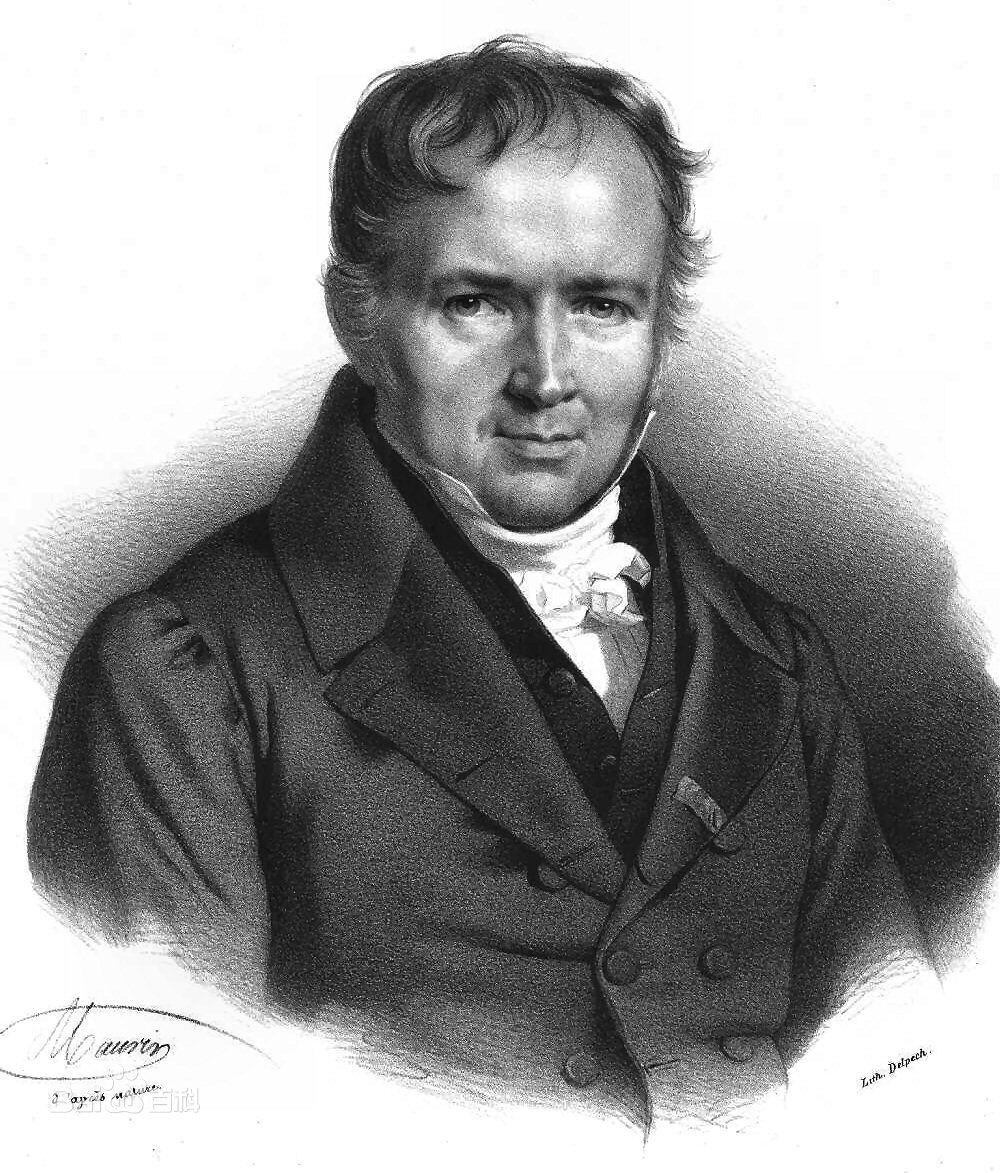
\includegraphics[width=4cm]{p1.jpg}
			\caption{泊松}
		\end{figure}
		\pause
		\column{6cm}
		\begin{itemize}[<+-|alert@+>]
			\item 西莫恩・德尼・泊松:法国数学家、几何学家和物理学家;
			      % \item 1781 年 6 月 21 日生于法国卢瓦雷省的皮蒂维耶,1840 年 4 月 25 日卒于法国索镇;
			\item 泊松的科学生涯开始于研究微分方程及其在摆的运动和声学理论中的应用;
			\item 对积分理论、行星运动理论、热物理、电磁理论、位势理论和概率论都有重要贡献;
			\item 19 世纪概率统计领域里的卓越人物,改进了概率论的运用方法,特别是用于统计方面的方法,建立了描述随机现象的一种概率分布──泊松分布;
			\item 推广了 “大数定律”,并导出了在概率论与数理方程中有重要应用的泊松积分。
		\end{itemize}


	\end{columns}
\end{frame}

\begin{frame}
	\frametitle{泊松 (Poisson) 分布}
	\begin{itemize}[<+-|alert@+>]
		\item Poisson 分布是概率论中一种重要的离散型分布,它在理论与实践中都有广泛的应用,常与单位时间 (面积) 内上的计数过程相联系;
		      \begin{itemize}
			      \item 一天内到达某商场的顾客数;
			      \item 单位时间内,电路受外界电磁波的冲击次数;
			      \item 一定时期内,某放射性物质放射出来的粒子数等
		      \end{itemize}
		\item 在二项分布中,当参数 $n$ 较大时,计算二项概率 $b (k;n,p)$ 会非常麻烦.
	\end{itemize}
	\pause  \begin{thm}
		设有一列二项分布 $\{b (k;n,p_n)\}$, 若其参数列 $p_n$ 满足
		\begin{eqnarray*}
			\lim_{n\rightarrow \infty}np_n=\lambda>0,
		\end{eqnarray*}
		则对任何非负整数 $k$ 有
		\begin{eqnarray*}
			\lim_{n\rightarrow \infty}b(k;n,p_n)=\dfrac{\lambda^k}{k!}e^{-\lambda}.
		\end{eqnarray*}
	\end{thm}
\end{frame}
\begin{frame}

	\vspace{0.4cm}
	\zheng 记 $\lambda_n:=np_n$, 则
	\begin{eqnarray*}
		b(k;n,p_n)&=&\pause C_n^kp_n^k(1-p_n)^{n-k}=\pause \dfrac{n!}{k!(n-k)!}(\dfrac{\lambda_n}{n})^k(1-\dfrac{\lambda_n}{n})^{n-k}\\
		&=&\pause \dfrac{\lambda_n^k}{k!}(1-\dfrac{1}{n})(1-\dfrac{2}{n})\cdots(1-\dfrac{k-1}{n})(1-\dfrac{\lambda_n}{n})^{n-k}
	\end{eqnarray*}
	\pause 注意到
	\begin{eqnarray*}
		&&\pause \lim_{n\rightarrow\infty}\lambda_n^k=\lambda^k, \\
		&&\pause \lim_{n\rightarrow\infty}(1-\dfrac{1}{n})(1-\dfrac{2}{n})\cdots(1-\dfrac{k-1}{n})=1\\
		&&\pause \lim_{n\rightarrow\infty}(1-\dfrac{\lambda_n}{n})^{n-k}=\pause \lim_{n\rightarrow\infty}e^{(n-k)\ln(1-\dfrac{\lambda_n}{n})}\\
		&&=\pause e^{\lim_{n\rightarrow\infty}(n-k)\ln(1-\frac{\lambda_n}{n})}=\pause e^{\lim_{n\rightarrow\infty}(n-k)(-\frac{\lambda_n}{n}+o(\frac{1}{n}))}\\
		&&=\pause e^{\lim_{n\rightarrow\infty}(-\lambda_n+\frac{k\lambda_n}{n}+(n-k)o(\frac{1}{n}))}=\pause e^{-\lambda}
	\end{eqnarray*}
	\pause 从而 \vspace{-0.8cm}
	\begin{eqnarray*}
		\lim_{n\rightarrow\infty}b(k;n,p_n)=\dfrac{\lambda^k}{k!}e^{-\lambda}, k=0, 1, 2,\cdots
	\end{eqnarray*}

\end{frame}
\begin{frame}
	有了上述定理,当 $n$ 很大而 $p$ 很小时,可以用近似公式计算二项概率
	\begin{eqnarray*}
		b(k;n,p)\approx \dfrac{(np)^k}{k!}e^{-np}
	\end{eqnarray*}
	这里我们要求 $p$ 很小,为保证 $n$ 很大时,乘积 $np$ 有适度的大小.

	\pause  \begin{defi}[泊松分布] 对参数 $\lambda>0$, 记
		\begin{eqnarray*}
			p(k;\lambda)=\dfrac{\lambda^k}{k!}e^{-\lambda}, \quad k=0, 1,\cdots.
		\end{eqnarray*}
		\pause 易见 $p (k;\lambda)>0$ 且
		\begin{eqnarray*}
			\sum_{k=0}^\infty p(k;\lambda)=\sum_{k=0}^\infty \dfrac{\lambda^k}{k!}e^{-\lambda}=\pause e^\lambda e^{-\lambda}=1
		\end{eqnarray*}
		\pause 即 $\{p (k;\lambda)\}$ 可以看成离散型分布的密度,我们就把它称为以 $\lambda$ 为参数的泊松分布,记作 $P (\lambda)$.
	\end{defi}
\end{frame}
\begin{frame}
	\frametitle{泊松分布的性质}
	\begin{itemize}[<+-|alert@+>]
		\item 泊松分布列 $p (k;\lambda)$ 随 $k$ 变化情况与二项分布相似,事实上,考虑比值
		      \begin{eqnarray*}
			      \dfrac{p(k;\lambda)}{p(k-1;\lambda)}=\dfrac{\lambda^k(k-1)!e^{-\lambda}}{\lambda^{k-1}k!e^{-\lambda}}=\dfrac{\lambda}{k}, k\ge 1
		      \end{eqnarray*}
		      \begin{itemize}
			      \item 当 $k<\lambda$ 时有,$p (k;\lambda)>p (k-1;\lambda)$;
			      \item 当 $k>\lambda$ 时有,$p (k;\lambda)<p (k-1;\lambda)$;
			      \item 因此 $p (k;\lambda)$ 随 $k$ 先升后降,在 $m=[\lambda]$ 处达到最大值,而 $\lambda$ 为整数时,$p (k;\lambda)$ 在 $m=\lambda,\lambda-1$ 处同时取到最大值.
		      \end{itemize}
		\item 泊松分布在随机选择下的不变性:假设某块放射性物质在单位时间内发射出的粒子数 $X$ 服从 $P (\lambda)$ 分布。而每个粒子被记录下来的概率为 $p$ 即粒子有 $1-p$ 的概率被计数器遗漏,如果各粒子是否被记录相互独立,试求记录下的粒子数 $Y$ 的分布.
	\end{itemize}
\end{frame}
\begin{frame}
	\begin{eqnarray*}
		P(Y=k)&=&\pause \sum_{n=0}^\infty P(X=n, Y=k)=\pause \sum_{n=0}^\infty P(X=n) P(Y=k|X=n)\\
		&=&\pause \sum_{n=k}^\infty P(X=n) P(Y=k|X=n)=\pause \sum_{n=k}^\infty p(n;\lambda)B(k;n,p) \\
		&=&\pause \sum_{n=k}^\infty \dfrac{\lambda^n}{n!}e^{-\lambda}C_n^kp^k(1-p)^{n-k}=\pause \sum_{n=k}^\infty\dfrac{[\lambda(1-p)]^{n-k}}{(n-k)!}\dfrac{1}{k!}e^{-\lambda}(\lambda p)^k\\
		&=&\pause \dfrac{1}{k!}e^{-\lambda p}(\lambda p)^k\\
	\end{eqnarray*}
\end{frame}

\subsection{超几何分布}

\begin{frame}{超几何分布}
	假设某个罐子中有 $w$ 个白球和 $b$ 个黑球,考虑如下两种取球方式
	\begin{itemize}[<+-|alert@+>]
		\item 有放回的抓取 $n$ 个球
		      \begin{itemize}[<+-|alert@+>]
			      \item $X:=n$ 个球中白球的数量;
			            \vspace{0.1cm}
			      \item $X\sim B(n, \dfrac{w}{w+b})$
		      \end{itemize}

		\item 不放回的抓取 $n$ 个球
		      \begin{itemize}[<+-|alert@+>]
			      \item $X:=n$ 个球中白球的数量;
			      \item $X$ 服从超几何分布,记为 $X\sim H (w,b,n)$;
			      \item 易知
			            $$P(X=k)=\frac{C_w^kC_b^{n-k}}{C_{w+b}^n}:=h(k,w,b,n), k=0,1,\cdots,r,$$
			            其中 $r:=\min\{w,n\}$.
			      \item 若要验证以上给出的确实为一个概率分布列,只需注意到下面的组合等式成立
			            \begin{eqnarray*}
				            \sum_{k=0}^rC_w^kC_{b}^{n-k}=C_{w+b}^n
			            \end{eqnarray*}
		      \end{itemize}

	\end{itemize}
\end{frame}




\begin{frame}{超几何分布:两个例子}
	\begin{itemize}[<+-|alert@+>]
		\item 不合格品抽检问题
		      \begin{itemize}[<+-|alert@+>]
			      \item 设有 $N$ 件产品,其中有 $M$ 件不合格品,从中不放回的抽取 $n$ 件;
			      \item 令 $X:=n$ 件抽取的产品中不合格品的件数;
			      \item $X\sim H(M,N-M,n)$
		      \end{itemize}
		\item 麋鹿的捕获 - 再捕获问题
		      \begin{itemize}[<+-|alert@+>]
			      \item 森林中共有 $N$ 头麋鹿。某天,捕获了 $M$ 头麋鹿,标记后将这 $M$ 头麋鹿再放回野外.
			      \item 几天后,又重新随机地捕获 $n$ 头麋鹿。假设重新捕获的麋鹿也同样可能是之前捕获的麋鹿.
			      \item 令 $X:=$ 再次被捕获的麋鹿的数量;
			      \item $X\sim H(M,N-M,n)$;
			      \item 第一次捕获的 $M$ 头麋鹿相当于前面例子中白球的总数,第一次未捕获的 $N-M$ 头麋鹿相当于前面例子中黑球的总数,再次被捕获的 $n$ 头麋鹿相当于前面例子中抽样的数量.
		      \end{itemize}
	\end{itemize}
\end{frame}




\begin{frame}{超几何分布的适用基础}
	\begin{itemize}[<+-|alert@+>]
		\item 除上面例子外,超几何分布还可出现在许多情况下;
		\item 超几何分布的适用基础是总体根据两套标签进行分类:
		      \begin{itemize}[<+-|alert@+>]
			      \item 在罐子的示例中,每个球不是白色就是黑色 (第一套标签);
			      \item 每个球要么是样本要么不是样本 (第二套标签);
		      \end{itemize}
		\item 两套标签中至少有一个是被完全随机分配的 (在罐子的例子中,球是随机抽样的);
		\item $X$ 代表被两套标签都标记的数量:在罐子的例子中,关注的是既被抽样又是白色的球。
		\item $X$ 服从超几何分布.
	\end{itemize}
\end{frame}

\begin{frame}{超几何分布之间的对称性}
	\begin{thm}
		$X\sim H (w,b,n), Y\sim H (n,w+b-n,w)$, 则 $X$ 和 $Y$ 是同分布的.
	\end{thm}

	\pause
	\zheng
	\begin{itemize}[<+-|alert@+>]
		\item 考虑一个由 $w$ 个白球和 $b$ 个黑球充满的罐子,现在随机不放回地从罐子里抓取 $n$ 个球;
		\item 白球或者黑球看作第一套标签,有没有被抽取看作第二套标签;
		\item $X$ 表示抽取的样本球中白球的数量 $\sim H (w,b,n)$;
		\item 若将是否被抽取看作第一套标签,白球或者黑球看作第二套标签;
		\item $Y$ 表示所有白球中被抽中的数量 $\sim H (n,w+b-n,w)$;
		\item 显然 $X$ 和 $Y$ 都是表示被抽取的白球数量,所以它们有相同的分布;
		\item 也可以用代数的方法来检查 $X$ 和 $Y$ 是否具有相同的概率质量函数,即验证 $P (X=k)=P (Y=k)$.
	\end{itemize}
\end{frame}


\begin{frame}{二项分布与超几何分布}
	\begin{thm}
		如果 $X \sim B (n,p), Y \sim B (m,p)$, 且 $X$ 和 $Y$ 相互独立,则当给定条件 $X+Y=r$ 时,$X$ 的条件分布为超几何分布 $H (n,m,r)$.
	\end{thm}
	\vspace{0.5cm}
	%    \\ \hspace*{\fill} \\
	%   从另一个角度,二项分布可以看作是超几何分布的极端情况.
	%    \\ \hspace*{\fill} \\
	\vspace{0.5cm}
	\begin{thm}
		如果 $X \sim H (M,b,n)$, 且当 $N=M+b \rightarrow \infty$ 时 $p=\dfrac{M}{N}$ 保持不变,则 $X$ 的分布列 (概率质量函数) 收敛到 $B (n,p)$ 的分布列.
	\end{thm}

\end{frame}



\begin{frame}
	\frametitle{超几何分布的二项近似}
	注意到
	{\small \begin{align*}
		 & h(k;M,b,n)=\pause \dfrac{C_M^kC_b^{n-k}}{C_{M+b}^n}=\pause \dfrac{C_M^kC_{N-M}^{n-k}}{C_{N}^n}                                                                                                                                                                                \\
		 & =\dfrac{\dfrac{M!}{k!(M-k)!}\dfrac{(N-M)!}{(n-k)!(N-M-(n-k))!}}{\dfrac{N!}{n!(N-n)!}}                                                                                                                                                                                         \\
		 & =\pause \dfrac{n!}{k!(n-k)!}\dfrac{M!}{(M-k)!}\dfrac{(N-M)!}{(N-M-(n-k))!}\dfrac{(N-n)!}{N!}                                                                                                                                                                                  \\
		 & =\pause \dfrac{n!}{k!(n-k)!}\dfrac{M(M-1)\cdots (M-(k-1))}{N(N-1)\cdots (N-(k-1))} \dfrac{(N-M)\cdots (N-M-(n-k)+1)}{(N-k)\cdots (N-n+1)}                                                                                                                                     \\
		 & =\pause \dfrac{n!}{k!(n-k)!}\dfrac{\dfrac{M}{N}(\dfrac{M}{N}-\dfrac{1}{N})\cdots (\dfrac{M}{N}-\dfrac{(k-1)}{N})}{1(1-\dfrac{1}{N})\cdots (1-\dfrac{(k-1)}{N})} \dfrac{(1-\dfrac{M}{N})\cdots (1-\dfrac{M}{N}-\dfrac{(n-k)-1}{N})}{(1-\dfrac{k}{N})\cdots (1-\dfrac{n-1}{N})} \\
		 & \rightarrow \pause C_n^k\bigg(\dfrac{M}{N}\bigg)^k\bigg(1-\dfrac{M}{N}\bigg)^{n-k}=b(k;n,p)
	\end{align*}
	}
\end{frame}

 \title[概率论]{第十二讲:常见的连续型分布}

\institute[东南大学数学学院]{\large \textrm{Email: xzhangseu@seu.edu.cn} \\ \quad  \\
	\large 东南大学 \quad 数学学院 \\
	\vspace{0.3cm}
	%  \trc{公共邮箱: \textrm{zy.prob@qq.com}\\
	%    \hspace{-1.7cm}  密 \qquad 码: \textrm{seu!prob}}
}
\date{}


{ \setbeamertemplate{footline}{}
	\begin{frame}
		\titlepage
	\end{frame}
}

% \begin{frame}[plain]
%   \frametitle{目录}
%   \setcounter{tocdepth}{2}
%   \tableofcontents
% \end{frame}
\addtocounter{framenumber}{-3}  % 目录页不计算页码
%\section{随机变量}
\subsection{常见的连续型分布}
\begin{frame}
	\frametitle{均匀分布}
	\begin{defi}
		任给参数 $a<b$, 函数
		\begin{eqnarray*}
			p(x)=\dfrac{1}{b-a}, \quad a<x<b
		\end{eqnarray*}
		满足密度函数的两个性质即:$p (x)\ge 0$ 且 $\int_{-\infty}^\infty p (x) dx=1$. 我们称以上式中的 $p (x)$ 为密度的连续型分布为区间 $(a,b)$ 上的均匀分布,记作 $U (a,b)$.
	\end{defi}
	\pause

	\begin{itemize}[<+-|alert@+>]
		\item 易见,均匀分布的分布函数为
		      \begin{eqnarray*}
			      F(x)=\left\{
			      \begin{array}{ll}
				      0,                & x<a       \\
				      \dfrac{x-a}{b-a}, & a\leq x<b \\
				      1.                & x\ge b
			      \end{array}
			      \right.
		      \end{eqnarray*}
		\item 如果 $X$ 服从 $U (a,b)$ 分布,则对任何 $a\le x<y\le b$ 有
		      \begin{eqnarray*}
			      P(x<X\le y)=\pause \int_x^y\dfrac{1}{b-a}dt=\pause \dfrac{y-x}{b-a}
		      \end{eqnarray*}

	\end{itemize}

\end{frame}

\begin{frame}
	\begin{figure}[htbp]
		\centering
		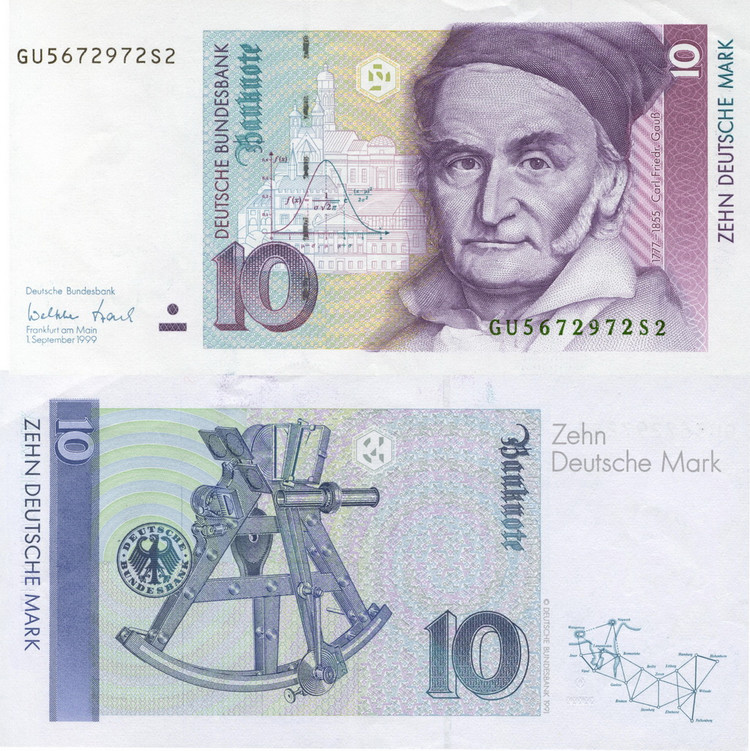
\includegraphics[width=8.5cm]{GaussMoney.jpg}
	\end{figure}
\end{frame}
% \setbeamertemplate{caption}[numbered]

\begin{frame}
	\begin{columns}
		\column{4cm}
		\begin{figure}[htbp]\nonumber
			\centering
			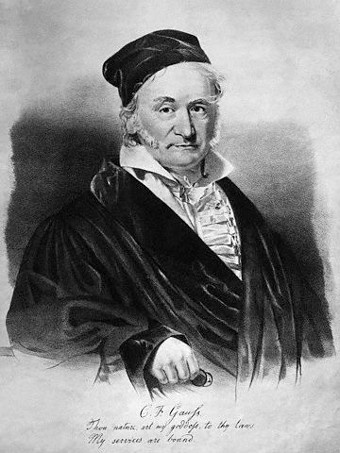
\includegraphics[width=5cm]{Gauss.jpg}
			\caption{高斯}
		\end{figure}
		\column{6cm}
		\begin{itemize}[<+-|alert@+>]
			\item 卡尔。弗里德里希。高斯 1777 年出生于布伦瑞克;
			\item 11 岁时就发现了二项式定理;
			\item 19 岁发现正十七边形的尺规作图法,解决了困扰数学家们两千多年的难题;
			\item 1809 年提出 “最小二乘法” 并在此基础上建立的正态分布方程,是概率统计中一个非常重要的工具,广泛应用于数学、物理学等领域;
			\item 一生发表了 155 篇论文,对数论、代数学、非欧几何、复变函数和微分几何等领域都做出了开创性的贡献,被誉为数学王子.
		\end{itemize}
	\end{columns}
\end{frame}
\begin{frame}
	\frametitle{正态分布 (高斯分布)}
	考虑下述函数
	\begin{eqnarray*}
		p_{\mu,\sigma}(x):=\dfrac{1}{\sqrt{2\pi}\sigma}e^{-\dfrac{(x-\mu)^2}{2\sigma^2}}
	\end{eqnarray*}
	\pause 下面我们验证 $p_{\mu,\sigma}(x)$ 满足密度函数的两个性质即非负性与正则性:非负性显然;正则性则需要计算积分 $I:=\int_{-\infty}^\infty p_{\mu,\sigma}(x) dx$.
\end{frame}

\begin{frame}
	\vspace{0.4cm}
	由于 $p_{\mu,\sigma}(x)$ 的原函数不是初等函数,我们无法通过微积分基本公式计算 $I$. 我们考虑计算 $I^2$:
	\begin{eqnarray*}
		I^2&=&\pause \int_{-\infty}^\infty \dfrac{1}{\sqrt{2\pi}\sigma}e^{-\dfrac{(x-\mu)^2}{2\sigma^2}}dx\int_{-\infty}^\infty \dfrac{1}{\sqrt{2\pi}\sigma}e^{-\dfrac{(x-\mu)^2}{2\sigma^2}}dx\\
		&=&\pause \int_{-\infty}^\infty \dfrac{1}{\sqrt{2\pi}\sigma}e^{-\dfrac{(x-\mu)^2}{2\sigma^2}}dx\int_{-\infty}^\infty \dfrac{1}{\sqrt{2\pi}\sigma}e^{-\dfrac{(y-\mu)^2}{2\sigma^2}}dy\\
		&=&\pause \int_{-\infty}^\infty\dfrac{1}{\sqrt{2\pi}}e^{-\dfrac{x^2}{2}}dx\int_{-\infty}^\infty\dfrac{1}{\sqrt{2\pi}}e^{-\dfrac{y^2}{2}}dy\\
		&=&\pause \dfrac{1}{2\pi}\int_{-\infty}^\infty\int_{-\infty}^\infty e^{-\dfrac{x^2+y^2}{2}}dxdy\\
		&=&\pause \dfrac{1}{2\pi}\int_0^{2\pi}\int_0^\infty e^{-\dfrac{r^2}{2}}rdrd\theta\\
		&=&\pause 1
	\end{eqnarray*}


\end{frame}
\begin{frame}
	\frametitle{正态分布的定义}
	\begin{defi}
		若随机变量 $X$ 的密度函数为
		\begin{eqnarray*}
			p_{\mu,\sigma}(x):=\dfrac{1}{\sqrt{2\pi}\sigma}e^{-\dfrac{(x-\mu)^2}{2\sigma^2}}
		\end{eqnarray*}
		则称 $X$ 服从参数为 $(\mu,\sigma^2)$ 的正态分布,记作 $X\sim N (\mu,\sigma^2)$. 特别的称 $N (0,1)$ 分布为标准正态分布,并简写 $p_{0,1}(x)$ 为 $\varphi (x)$. 正态分布又称高斯分布.
	\end{defi}
\end{frame}

\begin{frame}
	\frametitle{正态分布的性质}
	\begin{itemize}[<+-|alert@+>]
		\item 分布密度关于参数 $\mu$ 对称,即有
		      \begin{eqnarray*}
			      p_{\mu,\sigma}(\mu-x)=p_{\mu,\sigma}(\mu+x),  \quad \forall x \in R
		      \end{eqnarray*}
		      特别的,$N (0,1)$ 分布的密度函数为偶函数.
		\item $p_{\mu,\sigma}(x)$ 在 $x=\mu$ 处取得最大值 $\dfrac{1}{\sqrt{2\pi}\sigma}$. 注意到密度曲线下的面积应保持等于 1, 并且密度函数在 $x$ 处的值反映了此分布取值 $x$ 附近的概率大小。故 $\sigma^2$ 越小,密度的曲线越尖陡,分布取值越集中;$\sigma^2$ 越大,密度曲线越平缓,分布取值越分散.
		\item 正态分布的分布函数为
		      \begin{eqnarray*}
			      \Phi_{\mu,\sigma}(x)=\int_{-\infty}^x\dfrac{1}{\sqrt{2\pi}\sigma}e^{-\dfrac{(t-\mu)^2}{2\sigma^2}}dt
		      \end{eqnarray*}
		      特别的记标准正态分布函数为 $\Phi (x)$. 其与 $\Phi_{\mu,\sigma}(x)$ 有以下关系:
		      \begin{eqnarray*}
			      \Phi_{\mu,\sigma}(x)=\Phi(\dfrac{x-\mu}{\sigma})
		      \end{eqnarray*}
	\end{itemize}
\end{frame}
\begin{frame}
	\begin{exam}[3$\sigma$ 原则] 设随机变量 $X$ 服从 $N (\mu,\sigma^2)$ 分布,求 $P (|X-\mu|<3\sigma)$.
	\end{exam}

	\pause \jieda 注意到
	\begin{eqnarray*}
		P(|X-\mu|<3\sigma)&=&\pause P(\mu-3\sigma<X<\mu+3\sigma)\\
		&=&\pause \Phi_{\mu,\sigma}(\mu+3\sigma)-\Phi_{\mu,\sigma}(\mu-3\sigma)\\
		&=&\pause \Phi(3)-\Phi(-3)=\pause \Phi(3)-(1-\Phi(3))\\
		&=&\pause 2\Phi(3)-1=\pause 0.9973
	\end{eqnarray*}
	\pause 这表明,尽管正态分布的取值范围是 $(-\infty,+\infty)$, 但是其取值落在区间 $(\mu-3\sigma,\mu+3\sigma)$ 的概率高达 $99.73\%$


\end{frame}
\begin{frame}
	\frametitle{标准正态分布与一般正态分布之间的关系}
	\begin{exam}
		若 $X\sim N (\mu,\sigma^2)$, 则 $Y:=\dfrac{X-\mu}{\sigma}\sim N (0,1)$; 反之,若 $X\sim N (0,1)$, 则 $Y:=\sigma X+\mu\sim N (\mu,\sigma^2)$.
	\end{exam}

	\pause \jieda 我们仅给出第一种情况的证明。事实上,我们只需要说明 $Y$ 的分布密度为
	\vspace{-0.7cm}\begin{eqnarray*}
		\varphi(x)=\dfrac{1}{\sqrt{2\pi}}e^{-\dfrac{x^2}{2}}
	\end{eqnarray*}
	即可. \pause 事实上,考虑 $Y$ 的分布函数
	\begin{eqnarray*}
		F_Y(x)&=&\pause P(Y\le x)=\pause P(\dfrac{X-\mu}{\sigma}\le x)=\pause P(X\le \sigma x+\mu)\\
		&=&\pause \int_{-\infty}^{\sigma x+\mu}\dfrac{1}{\sqrt{2\pi}\sigma}e^{-\dfrac{(t-\mu)^2}{2\sigma^2}}dt=\pause \int_{-\infty}^x\dfrac{1}{\sqrt{2\pi}}e^{-\dfrac{y^2}{2}}dy
	\end{eqnarray*}
	\pause 从而 $Y$ 的分布密度为
	\begin{eqnarray*}
		p_Y(x)=F_Y'(x)=\dfrac{1}{\sqrt{2\pi}}e^{-\dfrac{x^2}{2}}=\varphi(x)
	\end{eqnarray*}
\end{frame}
\begin{frame}
	\frametitle{正态分布函数的简单性质}
	记 $\Phi (x)$ 为标准正态分布的分布函数,$U\sim N (0,1)$,  $\Phi_{\mu,\sigma}(x)$ 为 $N (\mu,\sigma^2)$ 分布的分布函数,$X\sim N (\mu,\sigma^2)$, 则 \pause
	\begin{itemize}[<+-|alert@+>]
		\item $\Phi(0)=\dfrac{1}{2}$;
		\item $\Phi_{\mu,\sigma}(\mu)=\dfrac{1}{2}$;
		\item $\Phi(-x)=1-\Phi(x)$;
		\item $P(|U|<x)=P(-x<U<x)=\pause P(U<x)-P(U\le -x)$ $=\pause \Phi(x)-(1-\Phi(x))=\pause 2\Phi(x)-1$;
		\item $\Phi_{\mu,\sigma}(x)=\pause P(X\le x)=\pause P(\dfrac{X-\mu}{\sigma}\le \dfrac{x-\mu}{\sigma})=\pause \Phi(\dfrac{x-\mu}{\sigma})$\pause
		\item $P(a<X\le b)=\Phi(\dfrac{b-\mu}{\sigma})-\Phi(\dfrac{a-\mu}{\sigma})$.
	\end{itemize}

\end{frame}
\begin{frame}
	\frametitle{伽玛函数 (Gamma 函数)}
	\begin{defi}
		称以下函数
		\begin{eqnarray*}
			\Gamma(\alpha):=\int_0^\infty x^{\alpha-1}e^{-x}dx, \quad \alpha>0,
		\end{eqnarray*}
		为 Gamma 函数.
	\end{defi}
	\pause
	Gamma 函数有以下性质:\pause
	\begin{itemize}[<+-|alert@+>]
		\item $\Gamma(1)=\pause \int_0^\infty x^{1-1}e^{-x}dx=\pause 1$;
		\item $\Gamma(\dfrac{1}{2})=\pause \int_0^\infty x^{\frac{1}{2}-1}e^{-x}dx=\pause 2\sqrt{\pi}\int_0^\infty \frac{1}{\sqrt{2\pi}}e^{-x}d\sqrt{2}x^{\frac{1}{2}}$ \pause $=2\sqrt{\pi}\int_0^\infty \frac{1}{\sqrt{2\pi}}e^{-\frac{t^2}{2}}dt=\pause \sqrt{\pi}$;
		\item $\Gamma (\alpha+1)=\alpha\Gamma (\alpha)$, 故 $\Gamma (n+1)=n\Gamma (n)=\cdots =n!$; \pause 事实上,
		      \begin{eqnarray*}
			      \Gamma(\alpha+1)&=&\pause \int_0^\infty x^\alpha e^{-x}dx=\pause \int_0^\infty -x^\alpha de^{-x}\\
			      &=&\pause -x^\alpha e^{-x}|_0^\infty+\int_0^\infty \alpha x^{\alpha-1} e^{-x}dx=\pause \alpha\Gamma(\alpha)
		      \end{eqnarray*}
	\end{itemize}

\end{frame}
\begin{frame}
	\frametitle{伽玛分布}
	\begin{defi}[Gamma 分布]
		若随机变量 $X$ 的密度函数为
		\begin{eqnarray*}
			p(x)=\left\{
			\begin{array}{ll}
				\dfrac{\lambda^\alpha}{\Gamma(\alpha)}x^{\alpha-1}e^{-\lambda x}, & x\ge 0 \\
				0,                                                                & x<0
			\end{array}
			\right.
		\end{eqnarray*}
		则称 $X$ 服从参数为 $(\alpha,\lambda)$ 的 Gamma 分布,记作 $X\sim \Gamma (\alpha,\lambda)$.
	\end{defi}
\end{frame}

\begin{frame}
	\frametitle{指数分布与 $\chi^2$(卡方) 分布}
	\begin{defi}
		称 $\Gamma (1,\lambda)$ 分布为指数分布,其密度函数与分布函数分别为
		\begin{eqnarray*}
			p(x)=\left\{
			\begin{array}{ll}
				\lambda e^{-\lambda x}, & x\ge 0, \\
				0,                      & x<0.
			\end{array}
			\right.\quad
			F(x)=\left\{
			\begin{array}{ll}
				1- e^{-\lambda x}, & x\ge 0, \\
				0,                 & x<0.
			\end{array}
			\right.
		\end{eqnarray*}

	\end{defi}
	\pause

	\begin{defi}
		称 $\Gamma (\frac{n}{2},\frac{1}{2})$ 分布为 $\chi^2$ 分布,记作 $\chi^2 (n)$, 其密度函数为
		\begin{eqnarray*}
			p(x)=\left\{
			\begin{array}{ll}
				\dfrac{1}{2^{\frac{n}{2}}\Gamma(\frac{n}{2})}x^{\frac{n}{2}-1}e^{-\frac{x}{2}}, & x\ge 0, \\
				0,                                                                              & x<0.
			\end{array}
			\right.
		\end{eqnarray*}

	\end{defi}
\end{frame}

\begin{frame}
	\frametitle{泊松分布与伽玛分布}
	\begin{exam}
		假定有一个于随机时刻陆续到来的质点流,我们若以 $N (t)$ 表示在 $[0,t]$ 时间内到来的质点的个数,并假设其服从参数为 $\lambda t$ 的泊松分布。试证明第 $n$ 个质点到达的时间 $S_n$ 服从 $\Gamma (n,\lambda)$ 分布.
	\end{exam}

	\pause
	\zheng 首先我们考虑一下 $S_n$ 的分布函数
	\begin{eqnarray*}
		P(S_n\le t)&=&\pause P(N(t)\ge n)=\pause \sum_{k=n}^\infty P(N(t)=k)\\
		&=&\sum_{k=n}^\infty \dfrac{(\lambda t)^k}{k!}e^{-\lambda t}
	\end{eqnarray*}
	\pause 故其密度 $p (t)$ 为
	\begin{eqnarray*}
		p(t)=F'(t)&=&\pause \sum_{k=n}^\infty\left[ \dfrac{\lambda(\lambda t)^{k-1}}{(k-1)!}e^{-\lambda t} - \dfrac{\lambda(\lambda t)^k}{k!}e^{-\lambda t}\right]\\
		&=& \pause \dfrac{\lambda(\lambda t)^{n-1}}{(n-1)!}e^{-\lambda t}=\pause \dfrac{\lambda^n}{\Gamma(n)}t^{n-1}e^{-\lambda t}
	\end{eqnarray*}

\end{frame}



% \input{ProbChap1.tex}

% \input{ProbChap2.tex}
% \input{ProbChap3.tex}
%  \input{ProbChap4.tex}




%%% Local Variables:
%%% mode: latex
%%% TeX-master: t
%%% End:


 




\title[概率论]{第十三讲:多维概率分布}
%\author[张鑫 {\rm Email: x.zhang.seu@foxmail.com} ]{\large 张 鑫}
\institute[东南大学数学学院]{\large \textrm{Email: xzhangseu@seu.edu.cn} \\ \quad  \\
	\large 东南大学 \quad 数学学院 \\
	\vspace{0.3cm}
	% \trc{公共邮箱: \textrm{zy.prob@qq.com}\\
		%    \hspace{-1.7cm}  密 \qquad 码: \textrm{seu!prob}}
}
\date{\rm \today}

{ \setbeamertemplate{footline}{}
  \begin{frame}
    \titlepage
  \end{frame}
}

% \begin{frame}[plain]
%   \frametitle{目录}
%   \setcounter{tocdepth}{2}
%   \tableofcontents
% \end{frame}
\addtocounter{framenumber}{-3}  % 目录页不计算页码
%\section{随机变量}
\subsection{多维概率分布}
\begin{frame}
  \frametitle{$n$ 维随机向量的定义}
  \begin{defi}[$n$ 维随机向量或随机变量] 如果 $X_1,\cdots, X_n$ 是定义在同一个概率空间 $(\Omega,\mathcal{F},P)$ 上的 $n$ 个随机变量,即
    \begin{eqnarray*}
      \{\omega:X_i (\omega)\in B_i\}\in \mathcal{F}, \quad \mbox{任意的} B_i\in \mathcal{B},
    \end{eqnarray*}
    则称 $X (\omega):=(X_1 (\omega),\cdots,X_n (\omega))$ 为概率空间 $(\Omega,\mathcal{F},P)$ 上的 $n$ 维随机向量或 $n$ 维随机变量.
  \end{defi}

\vspace{0.2cm}
\begin{rmk}
	\begin{itemize}[<+-|alert@+>]
		\item 如果 $\left (X_1,\cdots ,X_n \right) $ 是一个 $n$ 维随机向量,则对任何不超过 $n$ 的正整数 $k$ 和 $1\leqslant j_1<\cdots <j_k\leqslant n$, $\left ( X_{j_1},\cdots ,X_{j_k} \right) $
		都是一个 $k$ 维随机向量;
		\item 特别地,当 $k=1$ 时就是随机变量.
	\end{itemize}

\end{rmk}

\end{frame}
\begin{frame}{$n$ 维随机向量的定义}


	\begin{thm}
		$X (\omega)=(X_1 (\omega),\cdots,X_n (\omega))$ 是定义在某个概率空间 $(\Omega,\mathcal{F},P)$ 上的 $n$ 维随机向量当且仅当对任意的 $(x_1,\cdots, x_n)\in \mathbb{R}^ n$ 均有
		\[\{\omega: X_1(\omega)\leq x_1,\cdots, X_n(\omega)\leq x_n\}=\{X_1\leq x_1,\cdots, X_n\leq x_n\}\in\mathcal{F},\]
		或等价的有对任意的 $B\in\mathcal{B}(\mathbb{R}^ n)$
		\[\{\omega: X(\omega)\in B\}=\{\omega: (X_1(\omega),\cdots,X_n(\omega))\in B\}\in\mathcal{F}.\]
	\end{thm}


\end{frame}

\subsection{多维分布}
\begin{frame}{多维分布及联合分布函数}
		\begin{defi}[多维分布]
		设 $X=\left (X_1,\cdots ,X_n \right) $ 是定义在某个概率空间 $\left ( \varOmega ,\mathcal{F},P   \right) $ 上的 $n$ 维随机向量,则对任意的 $B\in\mathcal{B}(\mathbb{R}^n)$, 称
		$$
		\mathbf{F}(B):=P(X\in B)=P((X_1,\cdots, X_n)\in B)
		$$ 为 $n$ 维随机向量 $X=\left (X_1,\cdots ,X_n \right)$ 的分布. % 为其分布函数,也称为随机变量 $ X_1,\cdots ,X_n$ 的联合分布函数.
	\end{defi}

\pause

	\begin{defi}[分布函数或联合分布函数]
		设 $X=\left (X_1,\cdots ,X_n \right) $ 是定义在某个概率空间 $\left ( \varOmega ,\mathcal{F},P \right) $ 上的 $n$ 维随机向量,称
		$$
		F\left( x_1,\cdots ,x_n \right) =P\left( X_1\leqslant x_1,\cdots ,X_n\leqslant x_n \right) ,\quad \forall \left( x_1,\cdots ,x_n \right) \in \mathbb{R}^n
		$$ 为随机向量 $X$ 的分布函数,也称为随机变量 $ X_1,\cdots,X_n$ 的联合分布函数.
	\end{defi}
\pause
\begin{rmk}
\begin{itemize}[<+-|alert@+>]
	\item $n$ 维随机向量的分布函数 $F (x_1,\cdots,x_n)$ 是定义在 $\mathbb{R}^n$ 上的 $n$ 元函数;
	\item 称一个 $n$ 元函数 $F (x_1,\cdots,x_n)$ 为 $n$ 维分布函数,如果存在某个随机向量以它作为分布函数.
\end{itemize}
\end{rmk}

\end{frame}

\begin{frame}{$n$ 维随机向量分布函数的性质}
	\vspace{-0.15cm}
	\begin{thm}
	 	$n$ 维随机向量 $X=\left (X_1,\cdots ,X_n \right)$ 的分布函数 $F\left ( x_1,\cdots ,x_n \right)$ 具有下述性质:
		\begin{enumerate}[<+-|alert@+>]
			\item $F\left (x_1,\cdots ,x_n \right)$ 对每个变元非降;
			\item $F\left (x_1,\cdots ,x_n \right)$ 对每个变元右连续;
			\item 对任意的 $1\leq j\leq n$, $$
			\begin{aligned}
				&\lim_{x_j\rightarrow -\infty} F\left( x_1,\cdots, x_j,\cdots,x_n \right) =0,\\
				&\lim_{x_1\rightarrow \infty ,\cdots ,x_n\rightarrow \infty} F\left( x_1,\cdots ,x_n \right) =1\\
			\end{aligned}
			$$
			\item $F\left (x_1,\cdots ,x_n\right)$ 具有增量非负性:对任意的 $1\leq j\leq n$ 及 $a_j\leqslant b_j$ 均有 %,j=1,\cdots ,n,$ 都有
			$$
			\Delta_{\left(a_{1}, \cdots, a_{n}\right)}^{\left(b_{1}, \cdots, b_{n}\right)} F=\sum_{\boldsymbol{x}=(x_1,\cdots, x_n)\in\mathcal{O}} \operatorname{sgn}(\boldsymbol{x}) F(\boldsymbol{x}) \geqslant 0,
			$$
			其中 \vspace{-0.5cm}
			\begin{align*}
				\mathcal{O}&:=\{(x_1,\cdots,x_n): x_j=a_j\mbox{或} b_j, 1\leq j\leq n\},\\
				\operatorname{sgn}(\boldsymbol{x})&=\left\{
				\begin{array}{ll}
					1,& |\{j:x_j=a_j\}|\mbox{为偶数},\\
					-1, &|\{j:x_j=a_j\}|\mbox{为奇数}.
					\end{array}\right.
			\end{align*}
%			其中共有 $2^n$ 个加项,$\boldsymbol{x}=\left ( x_1,\cdots ,x_n \right) $,有 $x_j=a_j$ 或 $b_j,j=1,\cdots ,n,$,并且当 $\sharp \left\{ j\mid x_j=a_j \right\} $ 为偶数时,${sgn}(\boldsymbol{x})$ 为 $+$ 号,当 $\sharp \left\{ j\mid x_j=a_j \right\} $ 为奇数时,${sgn}(\boldsymbol{x})$ 为 $-$ 号,其中 $\sharp \left\{ \cdot \right\} $ 表示集合 $\left\{ \cdot \right\} $ 中的元素个数.
		\end{enumerate}
	\end{thm}

\end{frame}
\begin{frame}{$n$ 维随机向量分布函数的性质}

特别的,当 $n=2$ 或 3 时,$\Delta_{\left (a_{1}, \cdots, a_{n}\right)}^{\left (b_{1}, \cdots, b_{n}\right)} F$ 有以下具体形式:
\begin{align*}
	\Delta_{\left(a_{1}, a_{2}\right)}^{\left(b_{1}, b_{2}\right)} F&= F\left(b_{1}, b_{2}\right)-F\left(a_{1}, b_{2}\right)-F\left(b_{1}, a_{2}\right)+F\left(a_{1}, a_{2}\right) \pause \\
	\Delta_{\left(a_{1}, a_{2}, a_{3}\right)}^{\left(b_{1}, b_{2}, b_{3}\right)} F&= F\left(b_{1}, b_{2}, b_{3}\right)-F\left(a_{1}, b_{2}, b_{3}\right)-F\left(b_{1}, a_{2}, b_{3}\right)\\
	&\quad -F\left(b_{1}, b_{2}, a_{3}\right) +F\left(a_{1}, a_{2}, b_{3}\right)+F\left(a_{1}, b_{2}, a_{3}\right)\\
	&\quad +F\left(b_{1}, a_{2}, a_{3}\right)-F\left(a_{1}, a_{2}, a_{3}\right)
\end{align*}





\end{frame}


\begin{frame}
  \frametitle{二维 (联合) 分布函数}
  \begin{defi}
    设 $(X,Y)$ 为 $(\Omega,\mathcal{F},P)$ 上的随机向量,称
    \begin{eqnarray*}
      F(x,y):=P(X\le x, Y\le y)
    \end{eqnarray*}
    为 $(X,Y)$ 的二维 (联合) 分布函数.
  \end{defi}
  % \vspace{-1cm}
  \begin{figure}[h]
    \centering
    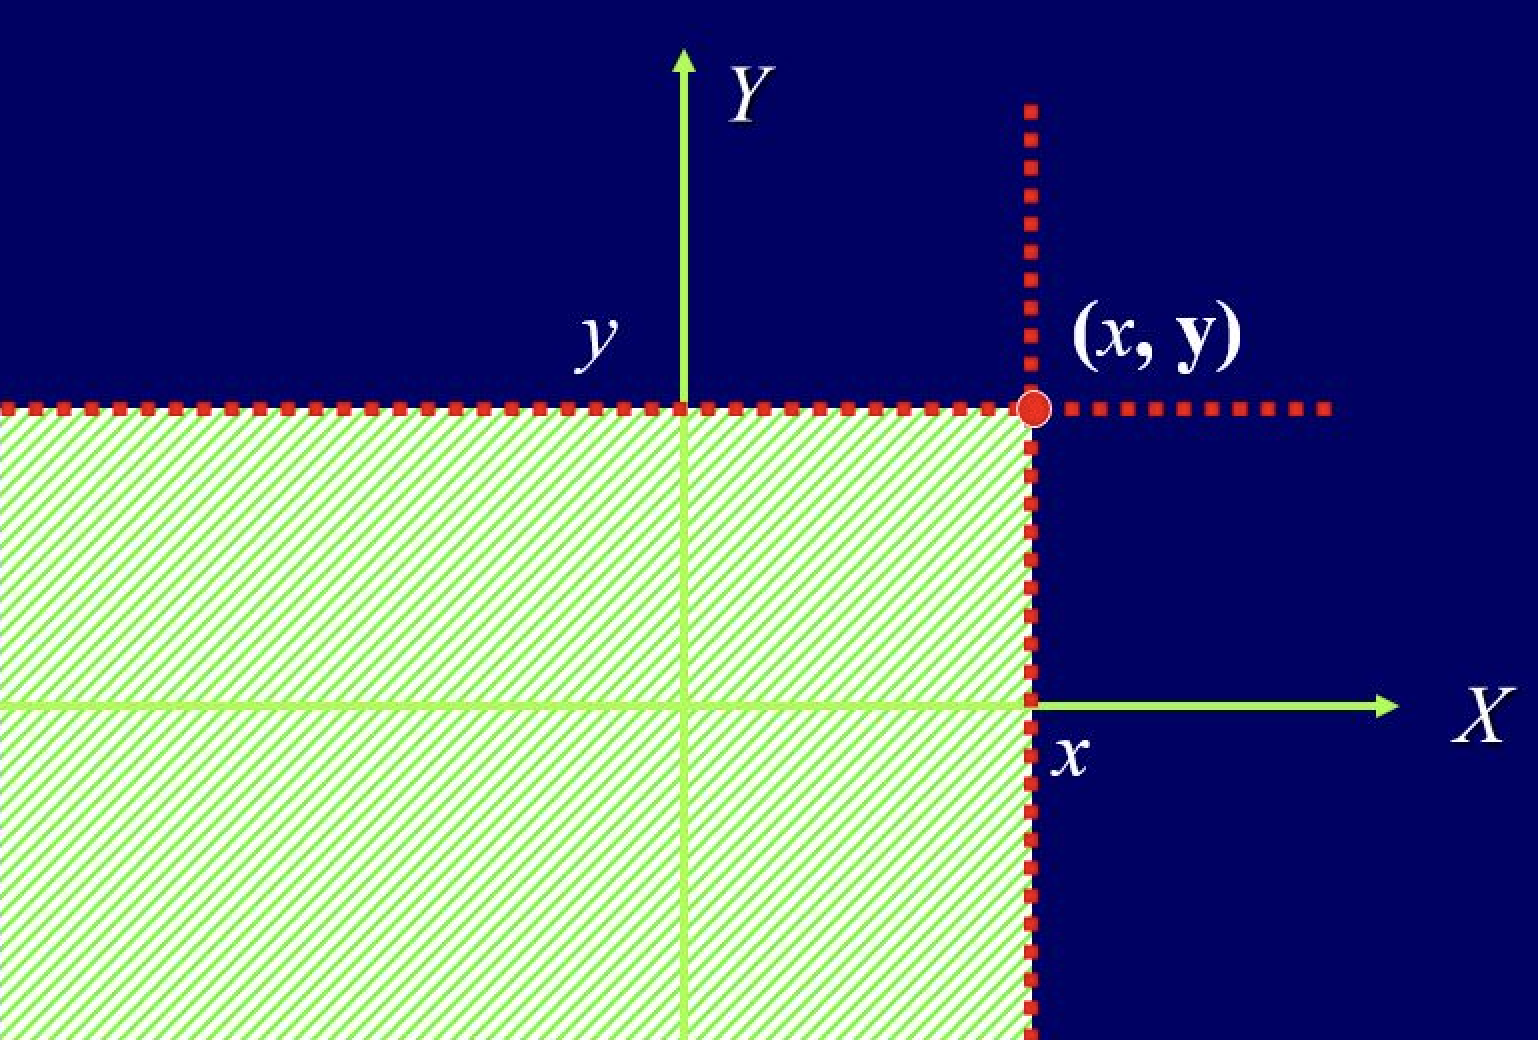
\includegraphics[width=7cm]{fxy.jpg}
    % \caption{高斯}
  \end{figure}

\end{frame}
\begin{frame}
  \frametitle{二维 (联合) 分布函数的性质}
  \begin{thm}
    $F (x,y)$ 具有性质
    \begin{enumerate}[<+-|alert@+>]
    \item $F (x,y)$ 对每个自变量是单调不减的;
    \item $F (x,y)$ 对每个自变量都是右连续的;
    \item{\small $\lim_{x\rightarrow -\infty}F(x,y)=\lim_{y\rightarrow -\infty}F(x,y)=1-\lim_{x\rightarrow +\infty, y\rightarrow +\infty }F(x,y)=0$;}
    \item $F (x,y)$ 在任一矩形 $(a_1,b_1]\times (a_2,b_2]$ 上具有非负增量,即有
      \begin{eqnarray*}
        \Delta F=F(b_1,b_2)-F(a_1,b_2)-F(b_1,a_2)+F(a_1,a_2)\ge 0.
      \end{eqnarray*}

    \end{enumerate}

  \end{thm}
\end{frame}
\begin{frame}
  \frametitle{二维离散型分布}
  \begin{defi}
    若随机向量 $(X,Y)$ 有至多可列对可能值 $(x_i,y_i), i,j=1,2,\cdots,$, 则称随机向量及其联合分布是离散型的,而
    \begin{eqnarray*}
      p_{ij}:=P(X=x_i,Y=y_j), \quad i, j=1,2,\cdots,
    \end{eqnarray*}
    称为 $(X,Y)$ 的联合分布列 (律). 我们常用下表来表示 $(X,Y)$ 的分布列
  \end{defi}
  % \vspace{-1cm}
  \begin{figure}[h]
    \centering
    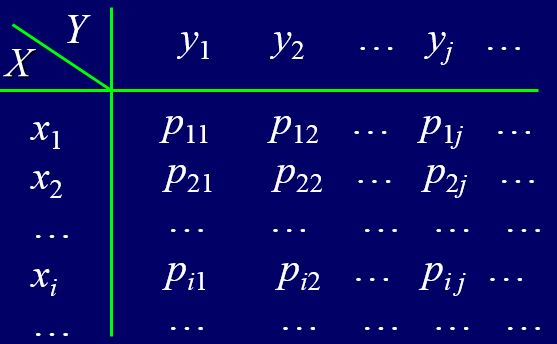
\includegraphics[width=6cm]{pij.jpg}
    % \caption{高斯}
  \end{figure}

\end{frame}
\subsection{二维离散及连续型分布}
\begin{frame}
  \frametitle{二维离散型分布列的基本性质}
  \begin{itemize}[<+-|alert@+>]
  \item 非负性: $p_{ij}\ge 0, i,j=1,2,\cdots $;
  \item 正则性: $\sum_i\sum_jp_{ij}=1$;
  \item 与一维情形类似,对任意的 $B\in \mathcal{B}^2$,
    \begin{eqnarray*}
      P((X,Y)\in B)=\sum_{i, j: (x_i,y_j)\in B}p_{ij}.
    \end{eqnarray*}

  \end{itemize}
\end{frame}
\begin{frame}
  \frametitle{计算联合分布列的方法}
  \begin{itemize}[<+-|alert@+>]
  \item 确定随机变量 $(X, Y)$ 的所有取值数对;
  \item 计算取每个数值对的概率;
  \item 列出表格
  \end{itemize}
  \pause
  \begin{exam}
    从 $1,2,3,4$ 中任取一数记为 $X$, 再从 $1,\cdots,X$ 中任取一数记作 $Y$, 求 $(X,Y)$ 的联合分布列及 $P (X=Y)$.
  \end{exam}
\end{frame}
\begin{frame}
  \frametitle{二维连续型分布}
  \begin{defi}
    若存在二元非负可积函数 $p (x,y)$ 使得 $(X,Y)$ 的二维 (联合) 分布函数
    \begin{eqnarray*}
      F(x,y)=\int_{-\infty}^x\int_{-\infty}^yp(u,v)dudv, \forall (x,y)\in\mathbb{R}^2
    \end{eqnarray*}
    则称 $(X,Y)$ 及其概率分布为连续型的,称 $p (x,y)$ 为其联合分布密度.
  \end{defi}
  \vspace{0.5cm}

  \pause
  易知,联合分布密度具有以下两个基本性质:
  \begin{enumerate}[<+-|alert@+>]
  \item 非负性: $p (x,y)\ge 0$;
  \item 正则性: $\int_{-\infty}^\infty\int_{-\infty}^\infty p (x,y) dxdy=1$.
  \end{enumerate}



\end{frame}
\begin{frame}
  \frametitle{联合分布密度与概率分布之间的关系}

  \begin{itemize}[<+-|alert@+>]
  \item $p(x,y)=\dfrac{\partial^2F(x,y)}{\partial x\partial y}$
  \item 对于连续型随机变量,对任意的 $B\in \mathcal{B}^2$ 有
    \begin{eqnarray*}
      P((X,Y)\in B)=\iint_Bp(x,y)dxdy
    \end{eqnarray*}

  \end{itemize}

\end{frame}
\begin{frame}

  \begin{exam}
    设 $(X,Y)$ 的联合密度函数为
    \begin{eqnarray*}
      p(x,y)=\left\{
      \begin{array}{ll}
        Ae^{-2x-3y},& x>0,y>0\\
        0,&\mbox{其他}
      \end{array}\right.
    \end{eqnarray*}
    试确定常数 $A$, 并求概率 $P (X<2,Y<1)$ 及 $P (2X+3Y<6)$.
  \end{exam}

  \jieda
  \begin{itemize}[<+-|alert@+>]
  \item 由 $\iint p (x,y) dxdy=1$ 可得 $A=6$;
  \item $P(X<2,Y<1)=\pause \int_{-\infty}^2\int_{-\infty}^1p(x,y)dxdy=\pause \int_0^2\int_0^1p(x,y)dxdy=\pause (1-e^{-4})(1-e^{-3})$;
  \end{itemize}

  % \vspace{-1.5cm}
  \begin{figure}[h]
    \centering
    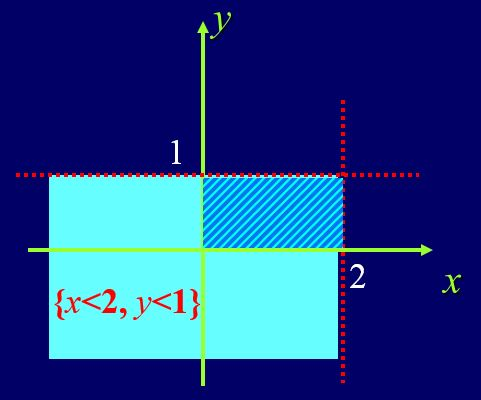
\includegraphics[width=4.8cm]{exam1.jpg}
    % \caption{高斯}
  \end{figure}
\end{frame}
\begin{frame}
  \vspace{0.8cm}
  注意到如果我们令 $D:=\{(x,y):2x+3y< 6\}$, 则
  \begin{eqnarray*}
    P(2X+3Y<6)&=&P((X,Y)\in D)=\iint_D p(x,y)dxdy\\
              &=&\int_0^3\int_0^{\frac{1}{3}(6-2x)}6e^{-(2x+3y)}dxdy\\
              &=&6\int_0^3e^{-2x}(-\frac{1}{3}e^{-3y})|_0^{\frac{1}{3}(6-2x)}dx=1-7e^{-6}
  \end{eqnarray*}

  % \vspace{-1.5cm}
  \begin{figure}[h]
    \centering
    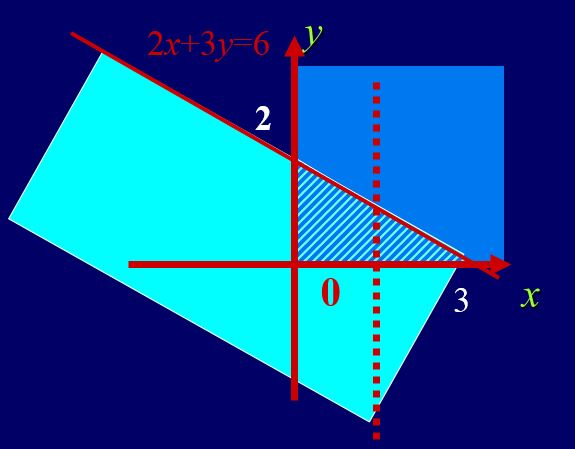
\includegraphics[width=5cm]{exam2.jpg}
  \end{figure}
\end{frame}

\subsection{边缘分布}
\begin{frame}
  \frametitle{边缘分布:随机向量的分量各自的概率分布}
  \begin{defi}[边缘分布] 在 $(X,Y)$ 的联合分布函数中,令 $y\uparrow +\infty$ 可得
    \begin{eqnarray*}
      \lim_{y\rightarrow+\infty}F(x,y)&=&\pause \lim_{y\rightarrow+\infty}P(X\le x, Y\le y)\\ &=& \pause P(X\le x,Y\le +\infty)=F(x,+\infty)
      \\
      &=&\pause P(X\le x):=F_1(x).    \end{eqnarray*}
  称 $F_1 (x)$ 为 $X$ 的边缘分布. \pause 类似的,$Y$ 的边缘分布为
\begin{eqnarray*}
F_2(y)=P(Y\le y)=\lim_{x\rightarrow+\infty}F(x,y)=F(+\infty,y)
\end{eqnarray*}

\end{defi}

\pause 从边缘分布的定义可知,若 $(X,Y)$ 的联合分布为 $F (x,y)$, 则
\begin{eqnarray*}
X\sim F_1(x)=F(x,+\infty)\\
Y\sim F_2(y)=F(+\infty, y)
\end{eqnarray*}
\end{frame}

\begin{frame}
	\frametitle{边缘分布的离散情形}
	\begin{itemize}[<+-|alert@+>]
		\item 边缘一词源于离散型情形。在二维离散型概率分布 $\{p_{ij}\}$ 的列表中,将各行求和写在表的最右一列,再将各列求和写在表的最下一行.
		\item 若 $(X,Y)$ 的联合分布列为 $\{p_{ij}\}$, 则 \pause %\vspace{-0.6cm}
		\begin{eqnarray*}
			&&X\mbox{的分布列为:} P (X=x_i)=\pause \sum_{j} P (X=x_i,Y=y_j)=\pause \sum_{j} p_{ij}=\pause p_{i\cdot};\\
			&& \pause Y\mbox{的分布列为:} P (Y=y_j)=\pause\sum_{i} P (X=x_i,Y=y_j)=\pause\sum_{i} p_{ij}=\pause p_{\cdot j}
		\end{eqnarray*}

	\end{itemize}
	\pause \vspace{-0.3cm}
	\begin{table}
		\centering
		\rowcolors[]{1}{blue!20}{blue!10}
		\begin{tabular}{|c|c|c|c|c|c|c|}
			\hline
			\rowcolor{blue!50}
			$i,j$ & 1  &2 &$\cdots$&$j$&$\cdots$ & $p_{i\cdot}$\\
			\hline
			1 & $p_{11}$ & $p_{12}$  & $\cdots$ &  $p_{1j}$& $\cdots$ & $p_{1\cdot}$\\
			2  & $p_{21}$ & $p_{22}$  &$\cdots$ &  $p_{2j}$  &$\cdots$ & $p_{2\cdot}$\\
			$\vdots$ & $\vdots$ & $\vdots$  &$\vdots$ &  $\vdots$ &$\vdots$& \\
			$i$ & $p_{i1}$ & $p_{i2}$  & $\cdots$ & $p_{ij}$ &$\cdots$ & $p_{i\cdot}$\\
			$\vdots$ & $\vdots$ & $\vdots$  &$\vdots$ &  $\vdots$ &$\vdots$& \\
			$p_{\cdot j}$& $p_{\cdot 1}$& $p_{\cdot 2}$& $\cdots$& $p_{\cdot j}$&$\cdots$& \\  \hline
		\end{tabular}
		% \caption{二维离散型分布列}
	\end{table}

\end{frame}
\begin{frame}
	\frametitle{边缘分布的连续情形}
	\begin{itemize}[<+-|alert@+>]
		\item 注意到
		\vspace{-0.4cm}\begin{eqnarray*}
			\hspace{-0.3cm}F_1(x)&=&P(X\le x)=\pause F(x,+\infty)=\pause \int_{-\infty}^x\int_{-\infty}^{+\infty}p(u,v)dudv\\
			&=&\pause \int_{-\infty}^x\underbrace{\left[\int_{-\infty}^{+\infty}p(u,v)dv\right]}_{p_1(u)}du=\pause \int_{-\infty}^xp_1(u)du
		\end{eqnarray*}
		\vspace{-0.4cm}   \pause  类似的有,\begin{eqnarray*}
			\hspace{-0.3cm}F_2(y)&=&P(Y\le y)=\pause F(+\infty,y)=\pause \int_{-\infty}^y\int_{-\infty}^{+\infty}p(u,v)dudv\\
			&=&\pause \int_{-\infty}^x\underbrace{\left[\int_{-\infty}^{+\infty}p(u,v)du\right]}_{p_2(v)}dv=\pause \int_{-\infty}^yp_2(v)dv
		\end{eqnarray*}
\item 对于连续型随机向量,其分量仍为连续型,相应的边缘密度分别为 $$p_1 (x)=\int_{-\infty}^{+\infty} p (x,y) dy,\quad  p_2 (y)=\int_{-\infty}^{+\infty} p (x,y) dx$$
\end{itemize}
\end{frame}
\subsection{常见的多维分布}
\begin{frame}
\frametitle{常见的多维离散型分布:多项分布}
\begin{itemize}[<+-|alert@+>]
\item 多项分布:进行 $n$ 次独立重复试验,每次试验有 $r$ 个互不相容的结果:$A_1,\cdots, A_r$ 之一发生;
\item 每次试验中 $A_i$ 发生的概率为 $p_i=P (A_i), i=1,\cdots,  r$ 且 $p_1+\cdots +p_r=1$;
\item 记 $X_i$ 为 $n$ 次独立试验中 $A_i$ 出现的次数,则 $(X_1,X_2,\cdots,X_r)$ 取值 $(n_1,n_2,\cdots,n_r)$ 的概率,即 $A_i,i=1,\cdots, r$ 出现 $n_i$ 次的概率为
\pause  \begin{eqnarray*}
	P(X_1=n_1,\cdots, X_r=n_r)=\dfrac{n!}{n_1!n_2!\cdots n_r!}p_1^{n_1}p_2^{n_2}\cdots p_r^{n_r}
\end{eqnarray*}
其中 $n=n_1+\cdots+n_r$;
\item 这个联合分布列称为 $r$ 项分布,又称多项分布,记作 $M (n,p_1,\cdots,p_r)$.
\item 上述概率是多项式 $(p_1+p_2+\cdots+p_r)^n$ 的一项,故其和为 1.
\item $r=2$ 时即为二项分布.
\end{itemize}
\end{frame}
\begin{frame}
	\frametitle{常见的多维离散型分布:多维超几何分布}
	\begin{itemize}
		\item 多维超几何分布:袋中有 $N$ 个球,其中有 $N_i$ 个 $i$ 号球,$i=1,2,\cdots, r$, 且 $N_1+N_2+\cdots +N_r=N$;
		\item 从中任取 $n$ 个球,若记 $X_i$ 为取出的 $n$ 个球中 $i$ 号球的个数,$i=1,2,\cdots, r$, 则 \pause
		\begin{eqnarray*}
			P(X_1=n_1,X_2=n_2,\cdots, X_r=n_r)=\dfrac{C_{N_1}^{n_1}C_{N_2}^{n_2}\cdots C_{N_r}^{n_r}}{C_{N}^n}
		\end{eqnarray*}
		其中 $n_1+n_2+\cdots+n_r=n$;
		\item $r=2$ 时即为超几何分布.\end{itemize}
\end{frame}
\begin{frame}
	\frametitle{多维均匀分布}
	\begin{defi}
		设 $D$ 为 $\mathbb{R}^ n$ 中的一个有界区域,其度量为 $S_D$, 如果多维随机变量 $(X_1,\cdots, X_n)$ 的联合密度函数为
		\begin{eqnarray*}
			p(x_1,\cdots,x_n)=\left\{
			\begin{array}{ll}
				\dfrac{1}{S_D}, &(x_1,x_2,\cdots,x_n)\in D\\
				0,&\mbox{其他}
			\end{array}\right.
		\end{eqnarray*}
		则称 $(X_1,\cdots,X_n)$ 服从 $D$ 上的多维均匀分布,记作 $(X_1,\cdots, X_n)\sim U (D)$.
	\end{defi}
	\vspace{0.5cm}

	\pause 二维均匀分布所描述的随机现象就是向平面区域 $D$ 中随机投点,如果该点的坐标 $(X,Y)$ 落在 $D$ 的子区域 $G$ 中的概率只与 $G$ 的面积有关,而与 $G$ 的位置无关,\pause 则
	\begin{eqnarray*}
		P((X,Y)\in G)=\iint_{G}p(x,y)dxdy=\iint_{G}\dfrac{1}{S_D}dxdy=\dfrac{S_G}{S_D}
	\end{eqnarray*}

\end{frame}
\begin{frame}
	\vspace{0.4cm}
	\begin{exam}
		设 $(X,Y)$ 服从单位圆 $D=\{(x,y):x^2+y^2<1\}$ 上的均匀分布,试求其边缘密度函数 (\textcolor{red}{非均匀分布}).
	\end{exam}
	\begin{columns}
		\pause   \column{3cm}
		% \vspace{-2cm}
		\begin{figure}[h]
			\centering
			\hspace{-1cm} 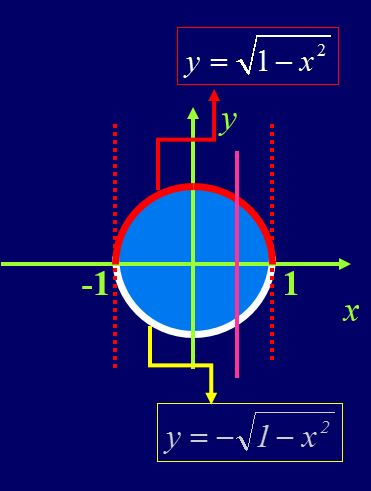
\includegraphics[width=4cm]{exam3.jpg}
		\end{figure}
		\pause %\vspace{0.7cm}
		\column{6.5cm}
		\pause $(X,Y)$ 的联合密度为
		\begin{eqnarray*}
			p(x,y)=\left\{
			\begin{array}{ll}
				\dfrac{1}{\pi}, & x^2+y^2<1\\
				0, & \mbox{其他}
			\end{array}\right.
		\end{eqnarray*}
		\pause 故当 $|x|\ge 1$, $p (x,y)=0$, 从而 $p_1 (x)=0$; 当 $|x|<1$ 时,
		\begin{eqnarray*}
			p_1(x)&=&\pause \int_{-\infty}^{+\infty}p(x,y)dy=\pause \int_{-\sqrt{1-x^2}}^{\sqrt{1-x^2}}\dfrac{1}{\pi}dy
			\\
			&=&\pause \dfrac{2}{\pi}\sqrt{1-x^2}
		\end{eqnarray*}\pause
		类似可得 $Y$ 的密度为 $p_2 (y)=\dfrac{2}{\pi}\sqrt{1-y^2}
		$
	\end{columns}
\end{frame}
\begin{frame}
	\frametitle{二维正态分布}
	\begin{defi}
		设参数 $\mu_1,\mu_2,\sigma_1,\sigma_2, \rho$ 满足 $\sigma_1>0,\sigma_2>0$ 及 $-1<\rho<1$, 称以
		\begin{eqnarray*}
			p(x,y)&=&\dfrac{1}{2\pi \sigma_1\sigma_2\sqrt{1-\rho^2}}\times\\
			&&\hspace{-1cm}\exp\bigg\{-\dfrac{1}{2(1-\rho^2)}\bigg[\dfrac{(x-\mu_1)^2}{\sigma_1^2}-\dfrac{2\rho(x-\mu_1)(y-\mu_2)}{\sigma_1\sigma_2}+\dfrac{(y-\mu_2)^2}{\sigma_2^2}\bigg]\bigg\}
		\end{eqnarray*}
		为密度函数的连续型分布为二维正态分布,记作 $$(X,Y)\sim N (\mu_1,\mu_2,\sigma_1^2,\sigma_2^2,\rho).$$
	\end{defi}

	\pause 后面我们会给出
	\begin{eqnarray*}
		\int_{-\infty}^{+\infty}  \int_{-\infty}^{+\infty}p(x,y)dxdy=1
	\end{eqnarray*}
	的证明.
\end{frame}

\begin{frame}
	\frametitle{二维正态分布密度图像}
	\vspace{0.2cm}
	\begin{figure}[h]
		\centering
		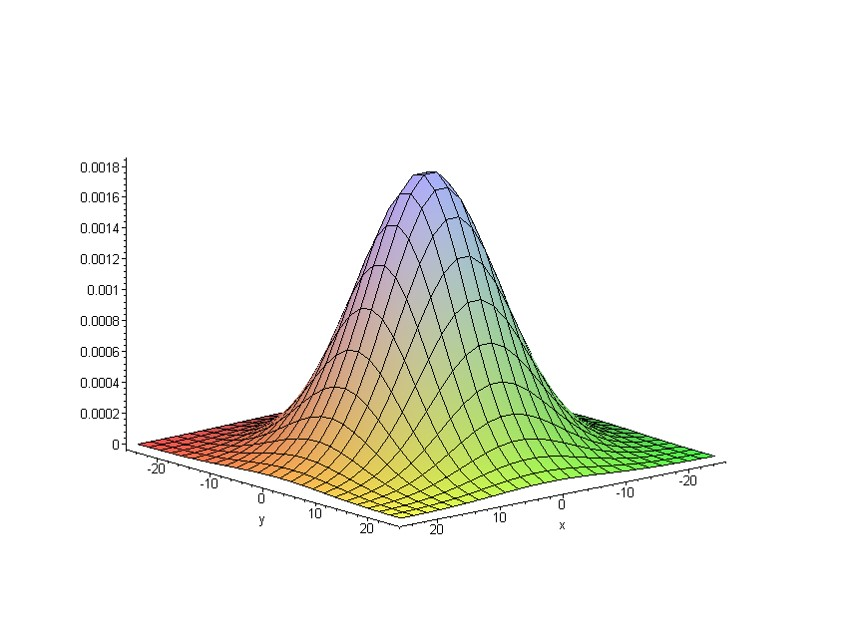
\includegraphics[width=11cm]{n2.jpg}
	\end{figure}
\end{frame}
\begin{frame}
	\frametitle{二维正态分布的边缘分布}
	\vspace{-0.3cm}
	\begin{thm}
		若 $(X,Y)$ 为二维正态分布 $N (\mu_1,\mu_2,\sigma_1^2,\sigma_2^2,\rho)$, 则 $$X\sim N (\mu_1,\sigma_1^2), \quad Y\sim N (\mu_2,\sigma_2^2)$$
	\end{thm}
	\vspace{-0.1cm}
	\pause\zheng $X$ 的边缘分布密度为
	{\small \begin{eqnarray*}
			p_1(x)&=&\pause \int_{-\infty}^{+\infty}\dfrac{1}{2\pi \sigma_1\sigma_2\sqrt{1-\rho^2}}\\
			&&\hspace{-0.3cm}\pause\cdot \exp\bigg\{-\dfrac{1}{2(1-\rho^2)}\bigg[\dfrac{(x-\mu_1)^2}{\sigma_1^2}-\dfrac{2\rho(x-\mu_1)(y-\mu_2)}{\sigma_1\sigma_2}+\dfrac{(y-\mu_2)^2}{\sigma_2^2}\bigg]\bigg\}dy\\
			&=&\pause \int_{-\infty}^{+\infty}\dfrac{1}{2\pi \sigma_1\sqrt{1-\rho^2}}\exp\left\{-\dfrac{u^2-2\rho uv+v^2}{2(1-\rho^2)}\right\}dv\\
			&=&\pause \int_{-\infty}^{+\infty}\dfrac{1}{2\pi \sigma_1\sqrt{1-\rho^2}}\exp\left\{-\dfrac{1}{2}\left[\left(\dfrac{v-\rho u}{\sqrt{1-\rho^2}}\right)^2+u^2\right]\right\}dv\\
			&=&\pause \dfrac{1}{\sqrt{2\pi}\sigma_1}e^{-\dfrac{(x-\mu_1)^2}{2\sigma_1^2}}\int_{-\infty}^{+\infty}\dfrac{1}{\sqrt{2\pi}} e^{-\dfrac{t^2}{2}}dt=\pause \dfrac{1}{\sqrt{2\pi}\sigma_1}e^{-\dfrac{(x-\mu_1)^2}{2\sigma_1^2}}
	\end{eqnarray*}}
	\pause 类似的可得 $Y\sim N (\mu_2,\sigma_2^2)$.
\end{frame}
%  \begin{frame}
	% \frametitle{作业}
	% P86-87. 习题 2.5.5: 3, 6, 7, 8, 9.
	%\end{frame}








\title[概率论]{第十四讲:条件分布与随机变量的独立性}
%\author[张鑫 {\rm Email: x.zhang.seu@foxmail.com} ]{\large 张 鑫}
\institute[东南大学数学学院]{\large \textrm{Email: xzhangseu@seu.edu.cn} \\ \quad  \\
	\large 东南大学 \quad 数学学院 \\
	\vspace{0.3cm}
%	\trc{公共邮箱: \textrm{zy.prob@qq.com}\\
	%	\hspace{-1.7cm}  密 \qquad 码: \textrm{seu!prob}}
}
\date{}





{ \setbeamertemplate{footline}{}
	\begin{frame}
		\titlepage
	\end{frame}
}
%\section{随机变量}
\subsection{条件分布}
\begin{frame}
	\frametitle{条件分布}
	\begin{itemize}[<+-|alert@+>]
		\item $(\Omega,\mathcal{F},P)$ 为一概率空间,任意固定 $B\in\mathcal{F}$ 且 $P (B)>0$, $P (\cdot|B)$ 仍为 $(\Omega,\mathcal{F})$ 上的概率;
		\item 对于 $(\Omega,\mathcal{F})$ 上的随机变量 $X$, 考虑其关于条件概率 $P (\cdot|B)$ 的分布即在概率空间 $(\Omega,\mathcal{F},P (\cdot|B))$ 上考虑 $X$ 的分布:
		\begin{eqnarray*}
			F(x|B):=P(X\le x|B)=\dfrac{P(X\le x, B)}{P(B)}, x\in R
		\end{eqnarray*}
		\item 现假定有另一随机变量 $Y$, 则当 $P (Y=y)>0$ 时,$F (x|Y=y)$ 则为已知 $Y=y$ 时 $X$ 的条件分布函数.
	\end{itemize}

\end{frame}

\begin{frame}
	\frametitle{离散型条件分布}
	\begin{defi}
		若离散型随机向量 $(X,Y)$ 的联合分布为 $\{p_{ij}\}$, 则当 $$P (Y=y_j)=p_{\cdot j}>0$$ 时,称
		\begin{eqnarray*}
			p_{i|j}:=P(X=x_i|Y=y_j)=\dfrac{p_{ij}}{p_{\cdot j}}, i=1,2,\cdots,
		\end{eqnarray*}
		为已知 $Y=y_j$ 时 $X$ 的条件分布. \pause 类似的,当 $P (X=x_i)=p_{i\cdot}>0$ 时,称
		\begin{eqnarray*}
			p_{j|i}:=P(Y=y_j|X=x_i)=\dfrac{p_{ij}}{p_{i\cdot}}
		\end{eqnarray*}
		为已知 $X=x_i$ 时 $Y$ 的条件分布.
	\end{defi}

\end{frame}
\begin{frame}
	\frametitle{离散型条件分布函数}
	根据上面的定义,给定 $Y=y_j$ 条件下 $X$ 的条件分布函数为
	\begin{eqnarray*}
		F(x|y_j)=\sum_{i:x_i\le x}P(X=x_i|Y=y_j)=\sum_{i:x_i\le x}p_{i|j}
	\end{eqnarray*}
	\pause 类似的给定 $X=x_i$ 条件下 $Y$ 的条件分布函数为
	\begin{eqnarray*}
		F(y|x_i)=\sum_{j:y_j\le y}P(Y=y_j|X=x_i)=\sum_{j:y_j\le y}p_{j|i}
	\end{eqnarray*}

\end{frame}
\begin{frame}
	\frametitle{连续型条件分布}
	\begin{itemize}[<+-|alert@+>]
		\item 设二维连续型随机变量 $(X,Y)$ 的联合密度函数为 $p (x,y)$, 边际密度函数分别为 $p_X (x), p_Y (y)$;
		\item 条件分布函数 $P (X\le x|Y=y)$: 因为 $P (Y=y)=0$, 故无法通过条件概率直接计算;
		\item $P(X\le x|Y=y):=\lim_{h\rightarrow 0}P(X\le x|Y\in[y,y+h])$;
		\item 根据如上定义:\vspace{-0.3cm}
		{\small \begin{eqnarray*}
				\hspace{-0.5cm} F(x|y)&:=&P(X\le x|Y=y)=\pause \lim_{h\rightarrow 0}\dfrac{P(X\le x, Y\in[y,y+h])}{P(Y\in[y,y+h])}\\
				&=&\pause \lim_{h\rightarrow 0}\dfrac{F(x,y+h)-F(x,y)}{F_Y(y+h)-F_Y(y)}
				=\pause \lim_{h\rightarrow 0}\dfrac{\big(F(x,y+h)-F(x,y)\big)/h}{\big(F_Y(y+h)-F_Y(y)\big)/h}\\
				&=&\pause \dfrac{\partial F(x,y)/\partial y}{p_Y(y)}
				%&&\hspace{-0.7cm}\pause \xlongequal[\mbox{积分中值定理}]{p (x,y),p_Y (y)\mbox{在} y\mbox{连续}}\pause \int_{-\infty}^x\dfrac{p (u,y)}{p_Y (y)} du\pause
		\end{eqnarray*}}%
		\item 故给定 $Y=y$ 时 $X$ 的条件分布密度为
		\begin{align*}
		   p (x|y)=\dfrac{\partial F(x|y)}{\partial x}=\dfrac{\partial^2 F(x,y)/[\partial x\partial y]}{p_Y(y)}=p(x,y)/p_Y (y).
		\end{align*}
	\end{itemize}
\end{frame}
\begin{frame}
	\frametitle{连续随机变量的条件分布函数及条件密度函数}
	\begin{defi}
		对一切使 $p_Y (y)>0$ 的 $y$, 给定 $Y=y$ 条件下 $X$ 的条件分布函数和条件密度函数分别为
		\begin{eqnarray*}
			F(x|y)&=&\int_{-\infty}^x\dfrac{p(u,y)}{p_Y(y)}du,\\
			p(x|y)&=&\dfrac{p(x,y)}{p_Y(y)}.
		\end{eqnarray*}
		同理,对一切使 $p_X (x)>0$ 的 $x$, 给定 $X=x$ 条件下 $X$ 的条件分布函数和条件密度函数分别为
		\begin{eqnarray*}
			F(y|x)&=&\int_{-\infty}^y\dfrac{p(x,v)}{p_X(x)}dv,\\
			p(y|x)&=&\dfrac{p(x,y)}{p_X(x)}.
		\end{eqnarray*}
	\end{defi}
\end{frame}
\begin{frame}
	\frametitle{连续场合的全概率公式和贝叶斯公式}
	\begin{itemize}[<+-|alert@+>]
		\item 由条件密度函数的定义可得
		\begin{eqnarray*}
			p(x,y)=p_X(x)p(y|x), \quad p(x,y)=p_Y(y)p(x|y)
		\end{eqnarray*}
		\item 对 $p (x,y)$ 求边际密度函数可得
		\begin{eqnarray*}
			p_X(x)&=&\pause \int_{-\infty}^{+\infty}p_Y(y)p(x|y)dy\pause \\
			\pause P(X\le x)&=&\pause \int_{-\infty}^x\bigg[\int_{-\infty}^{+\infty}p_Y(y)p(u|y)dy\bigg]du\\
			&=&\pause \int_{-\infty}^{+\infty}\bigg[\int_{-\infty}^xp(u|y)du\bigg]p_Y(y)dy\\
			&=&\pause \int_{-\infty}^{+\infty}P(X\le x|Y=y)dP(Y\le y)
			% p_Y(y)=\int_{-\infty}^{+\infty}p_X(x)p(y|x)dx, F(y)=\int_{-\infty}^{+\infty}\bigg[\int_{-\infty}^yp(v|x)dv\bigg]p_X(x)dx\\
		\end{eqnarray*}

	\end{itemize}
\end{frame}
\begin{frame}
	\frametitle{连续场合的全概率公式和贝叶斯公式}
	\begin{itemize}[<+-|alert@+>]
		\item 类似推导可得
		\begin{eqnarray*}
			p_Y(y)&=&\pause \int_{-\infty}^{+\infty}p_X(x)p(y|x)dx \\
			\pause P(Y\le y)&=& \pause \int_{-\infty}^{+\infty}P(Y\le y|X=x)dP(X\le x)
			% p_Y(y)=\int_{-\infty}^{+\infty}p_X(x)p(y|x)dx, F(y)=\int_{-\infty}^{+\infty}\bigg[\int_{-\infty}^yp(v|x)dv\bigg]p_X(x)dx\\
		\end{eqnarray*}
		\item 贝叶斯公式的密度函数形式:
		\begin{eqnarray*}
			p(x|y)=\dfrac{p(x,y)}{p_Y(y)}=\dfrac{p_X(x)p(y|x)}{\int_{-\infty}^{+\infty}p_X(x)p(y|x)dx}\\
			p(y|x)=\dfrac{p(x,y)}{p_X(x)}=\dfrac{p_Y(y)p(x|y)}{\int_{-\infty}^{+\infty}p_Y(y)p(x|y)dy}
		\end{eqnarray*}

	\end{itemize}
\end{frame}


\begin{frame}
	\begin{exam}
		若 $(X,Y)$ 为二维正态分布 $N (\mu_1,\mu_2,\sigma_1^2,\sigma_2^2,\rho)$, 试求给定 $Y=y$ 时 $X$ 的条件分布密度.\\
	\end{exam}


	\pause\jieda $X$ 的条件分布密度为
	\begin{eqnarray*}
		&&\hspace{-0.8cm}p(x|y)=\pause \dfrac{p(x,y)}{p_Y(y)}\\
		&=&\pause  \dfrac{\frac{1}{2\pi \sigma_1\sigma_2\sqrt{1-\rho^2}}\exp\big\{-\frac{1}{2(1-\rho^2)}\big[\frac{(x-\mu_1)^2}{\sigma_1^2}-\frac{2\rho(x-\mu_1)(y-\mu_2)}{\sigma_1\sigma_2}+\frac{(y-\mu_2)^2}{\sigma_2^2}\big]\big\}}{\frac{1}{\sqrt{2\pi}\sigma_2}\exp\big\{-\frac{(y-\mu_2)^2}{2\sigma_2^2}\big\}}\\
		&=&\pause \frac{\exp\big\{\frac{-1}{2\sigma_1^2(1-\rho^2)}\big[(x-\mu_1)^2-2\rho\frac{\sigma_1}{\sigma_2}(x-\mu_1)(y-\mu_2)+\rho^2\frac{\sigma_1^2}{\sigma_2^2}(y-\mu_2)^2\big]\big\}}{\sqrt{2\pi} \sigma_1\sqrt{1-\rho^2}}\\
		&=&\pause \frac{1}{\sqrt{2\pi} \sigma_1\sqrt{1-\rho^2}}\exp\big\{-\frac{1}{2\sigma_1^2(1-\rho^2)}\big[x-(\mu_1+\rho\frac{\sigma_1}{\sigma_2}(y-\mu_2)\big]^2\big\}\\
		&\sim&\pause  N(\mu_1+\rho\frac{\sigma_1}{\sigma_2}(y-\mu_2),\sigma_1^2(1-\rho^2)) \xlongequal{\rho=0} N(\mu_1,\sigma_1^2)
	\end{eqnarray*}
	\pause 类似可求得 $Y$ 关于 $X=x$ 的条件分布密度.
\end{frame}

\begin{frame}
	\begin{exam}
		设 $(X,Y)$ 服从单位圆 $D=\{(x,y):x^2+y^2<1\}$ 上的均匀分布,试求条件分布密度函数 $p (y|x)$.
	\end{exam}

	\jieda
	$(X,Y)$ 的联合密度及 $X$ 的边缘密度分别为
	\begin{eqnarray*}
		p(x,y)=\left\{
		\begin{array}{ll}
			\dfrac{1}{\pi}, & x^2+y^2<1,\\
			0, & \mbox{其他}
		\end{array}\right. ,\quad
		p_X(x)=\left\{\begin{array}{ll}
			\dfrac{2}{\pi}\sqrt{1-x^2}, & |x|<1,\\
			0, & \mbox{其他}.
		\end{array}\right.
	\end{eqnarray*}
	\pause 故
	\begin{eqnarray*}
		p(y|x)=\dfrac{p(x,y)}{p_X(x)}=\left\{
		\begin{array}{ll}
			\dfrac{1}{2\sqrt{1-x^2}}, & |y|\le \sqrt{1-x^2}\\
			0, &\mbox{其他}
		\end{array}
		\right.
	\end{eqnarray*}

\end{frame}


\subsection{随机变量的独立性}

\begin{frame}
	\frametitle{随机变量的独立性}
	\begin{itemize}[<+-|alert@+>]
		\item 首先我们回顾一下事件的独立性: $$P (AB)=P (A) P (B)\Leftrightarrow P (A|B)=P (A), \mbox{当} P (B)>0;$$
		\item 二维离散型随机变量
		\begin{eqnarray*}
			p_{i|j}:=\textcolor{red}{\dfrac{p_{ij}}{p_{\cdot j}}}=P (X=x_i|Y=y_j)\pause\xlongequal[\mbox{不影响概率}]{\mbox{若条件事件}} P (X=x_i)\textcolor{red}{=p_{i\cdot}};
		\end{eqnarray*}
		\item 故如果对任意的事件 $\{X=x_i\}, \{Y=y_j\}, i,j=1,2,\cdots,$ 均独立,我们则可称随机变量 $X,Y$ 独立,即 $X,Y$ 独立等价于
		\begin{eqnarray*}
			p_{ij}=p_{i\cdot}p_{\cdot j}, \quad i,j=1,2,\cdots,
		\end{eqnarray*}
		\item 此时的联合分布函数 $F (x,y)$ 为
		\begin{eqnarray*}
			\textcolor{red}{F(x,y)}&=&\pause P(X\le x,Y\le y)=\pause \sum_{x_i\le x}\sum_{y_j\le y}p_{ij}=\pause \sum_{x_i\le x}p_{i\cdot}\sum_{y_j\le y}p_{\cdot j}\\
			&=&\pause \sum_{x_i\le x}P(X=x_i)\sum_{y_j\le y}P(Y=y_j)=\pause \textcolor{red}{F_X(x)F_Y(y)}
		\end{eqnarray*}
	\end{itemize}
\end{frame}
\begin{frame}
	\frametitle{随机变量的独立性}
	\begin{itemize}[<+-|alert@+>]
		\item 二维连续型随机变量
		\begin{eqnarray*}
			F (x|y)&=&\int_{-\infty}^x\dfrac{p (u,y)}{p_Y (y)} du=P (X\le x|Y=y)\xlongequal[\mbox{不影响概率}]{\mbox{若条件事件}} P (X\le x)\\
			&=&\int_{-\infty}^xp_X(u)du\\
			&\Rightarrow& p(x,y)=p_X(x)p_Y(y)
		\end{eqnarray*}
		\item 此时,其分布函数
		\begin{eqnarray*}
			\textcolor{red}{F(x,y)}&=&P(X\le x, Y\le y)=\int_{-\infty}^x\int_{-\infty}^yp(u,v)dudv\\
			&=&\int_{-\infty}^xp_X(u)du\int_{-\infty}^yp_Y(v)dv=\textcolor{red}{F_X(x)F_Y(y)}
		\end{eqnarray*}
	\end{itemize}
\end{frame}
\begin{frame}
	\frametitle{随机变量独立性的定义}
	\begin{defi}
	 设 $n$ 维随机变量 $(X_1,X_2,\cdots,X_n)$ 的联合分布函数为 $F (x_1,
		\cdots,x_n)$, $F_i (x_i)$ 为 $X_i$ 的边缘分布函数。如果对任意的 $n$ 个实数 $x_1,x_2,\cdots, x_n$, 有
		\begin{eqnarray*}
			F(x_1,x_2,\cdots, x_n)=F_1(x_1)F_2(x_2)\cdots F_n(x_n)
		\end{eqnarray*}
		则称 $X_1,X_2,\cdots, X_n$ 相互独立。特别的,
	\end{defi}
	\pause
	\begin{enumerate}[<+-|alert@+>]
		\item 在离散随机变量场合,如果对任意 $n$ 个取值 $x_1,x_2,\cdots, x_n$, 有
		{\small     \begin{eqnarray*}
				P(X_1=x_1,X_2=x_2,\cdots,X_n=x_n)=P(X_1=x_1)P(X_2=x_2)\cdots P(X_n=x_n),
		\end{eqnarray*}}
		则称 $X_1,X_2,\cdots, X_n$ 相互独立.


		\item 在连续随机变量场合,如果对任意的 $n$ 个取值 $x_1,x_2,\cdots, x_n$, 有
		\begin{eqnarray*}
			p(x_1,x_2,\cdots, x_n)=p_1(x_1)p_2(x_2)\cdots p_n(x_n)
		\end{eqnarray*}
		则称 $X_1,X_2,\cdots, X_n$ 相互独立.
	\end{enumerate}
\end{frame}



 \title[概率论]{第十五讲:随机变量函数的分布}
% \author[张鑫 {\rm Email: x.zhang.seu@foxmail.com} ]{\large 张 鑫}
 \institute[东南大学数学学院]{\large \textrm{Email: xzhangseu@seu.edu.cn} \\ \quad  \\
 	\large 东南大学 \quad 数学学院 \\
 	\vspace{0.3cm}
 %	\trc{公共邮箱: \textrm{zy.prob@qq.com}\\
 	%	\hspace{-1.7cm}  密 \qquad 码: \textrm{seu!prob}}
 }
 \date{}



 	{ \setbeamertemplate{footline}{}
 		\begin{frame}
 			\titlepage
 		\end{frame}
 	}














% \section{随机变量}

 \subsection{随机变量函数的分布}
 \begin{frame}
 	\frametitle{一维离散型随机变量函数的分布}
 	\begin{thm}
 		设 $X\sim \{p_k\}$ 为一维离散型随机变量,若 $Z=f (X)$, 则对随机变量 $Z$ 的所有可能值 $z_k$ 有
 		\begin{eqnarray*}
 			P(Z=z_k)=\sum_{i:f(x_i)=z_k}p_i
 		\end{eqnarray*}
 	\end{thm}%
 	\pause%
 	\noindent\zheng 注意到 \vspace{-1cm}
 	\begin{eqnarray*}
 		\hspace{1.5cm} \{Z=z_k\}=\{f(X)=z_k\}=\cup_{i:f(x_i)=z_k}\{X=x_i\}
 	\end{eqnarray*}
 	\pause 故 $P (Z=z_k)=\sum_{i:f (x_i)=z_k} P (X=x_i)=\sum_{i:f (x_i)=z_k} p_i$.
 	\begin{exam}
 		若 $P (X=1)=P (X=-1)=0.25, P (X=0)=0.5$, 求 $Z=X^2$ 的分布.
 	\end{exam}

 	\jieda \pause$P(Z=1)=\sum_{i:x_i^2=1}p_i=P(X=1)+P(X=-1)=0.5$\\
 	\pause $$P(Z=0)=P(X=0)=0.5$$
 \end{frame}

 \begin{frame}
 	\frametitle{$Y=f (X): f (x)$ 严格单调且 $X$ 为连续型随机变量}
 	\begin{thm}
 		设 $X$ 是连续随机变量,其密度函数为 $p_X (x)$. $Y=f (X)$ 是另一个随机变量。若 $y=f (x)$ 严格单调,其反函数 $h (y)$ 有连续导数,则 $Y=f (X)$ 的密度函数为
 		\begin{eqnarray*}
 			p_Y(y)=\left\{
 			\begin{array}{ll}
 				p_X(h(y))|h'(y)|,& a\leq y\leq b\\
 				0,&\mbox{其他}
 			\end{array}
 			\right.
 		\end{eqnarray*}
 		其中 $a=\min\{f (-\infty), f (+\infty)\}, b=\max\{f (-\infty), f (+\infty)\}$.
 	\end{thm}

 	\pause \zheng 由 $f (x)$ 为严格单调函数可知:%
 	\begin{eqnarray*}
 		\hspace{-0cm} F_Y(y)&=&\pause P(Y\le y)=P(f(X)\le y)\\
 		&=&\pause \left\{
 		\begin{array}{ll}
 			\pause 0, & y<a\\
 			\pause 1, & y>b\\
 			\pause P (X\le h (y))=\pause \int_{-\infty}^{h (y)} p_X (x) dx, & a\leq y \leq b \mbox{且} f (x)\mbox{严格递增}\\
 			\pause P (X\ge h (y))=\pause \int_{h (y)}^{+\infty} p_X (x) dx, &a\leq y \leq b\mbox{且} f (x)\mbox{严格递减}
 		\end{array}
 		\right.
 	\end{eqnarray*}

 \end{frame}

 % \begin{frame}
 	%   从而 $Y$ 的密度函数为
 	%   \begin{eqnarray*}
 		%       p_Y(y)=\left\{
 		%       \begin{array}{ll}
 			%       p_X(h(y))|h'(y)|,& a<y<b\\
 			%       0,&\mbox{其他}
 			%     \end{array}
 		%                   \right.
 		%     \end{eqnarray*}

 	%                   \end{frame}
 \begin{frame}
 	\frametitle{几个常见的函数形式 $f$}
 	\begin{itemize}[<+-|alert@+>]
 		\item $f (x)=ax+b$ : 当 $X$ 为均匀分布,正态分布,伽玛分布时,求 $Y=f (X)$ 的分布密度;
 		\item 当 $X\sim N (\mu,\sigma^2)$ 时,可以验证 $aX+b\sim N (a\mu+b, a^2\sigma^2)$;
 		\item $f (x)=e^x$ : 当 $X$ 为均匀分布,正态分布,伽玛分布时,\\ 求 $Y=f (X)$ 的分布密度;
 		\item 对无单调性的函数 $f (x)$, 我们一般根据 $X$ 的分布密度想法求出 $Y$ 的分布函数 $F_Y (y)$,
 		\begin{eqnarray*}
 			F_Y(y)&=&P(Y\le y)=P(f(X)\le y)=P(X\in f^{-1}((-\infty, y]))\\
 			&=&\int_{f^{-1}((-\infty, y])}p_X(x)dx
 		\end{eqnarray*}
 		\item 然后对 $F_Y (y)$ 关于 $y$ 求导即可得到其分布密度 $p_Y (y)$.
 	\end{itemize}

 \end{frame}


% \begin{frame}
% 	\frametitle{两个问题}
% 	\begin{itemize}[<+-|alert@+>]
% 		\item 若 $X$ 为随机变量,对于怎样的 $f$ 才会有 $f (X)$ 仍然为随机变量?
% 		\item 给定分布函数 $F (x)$, 是否存在某个随机变量 $X$ 恰好使得其分布函数为给定的 $F (x)$?
% 	\end{itemize}
% \end{frame}
% \begin{frame}
% 	\frametitle{随机变量的 $p$ 分位数函数}
% 	\vspace{-0.3cm}
% 	\begin{defi}
% 		设 $X$ 是概率空间 $(\Omega,\mathcal{F},P)$ 上的随机变量,$F (x)$ 为其分布函数。对于 $p\in (0,1)$, 定义
% 		\begin{eqnarray*}
% 			F^{-1}(p):=\sup\{x:F(x)<p\}\pause =\inf\{x: F(x)\geq p\}.
% 		\end{eqnarray*}
% 		称 $F^{-1}(p)$ 为 $F$ 或 $X$ 的 $p$ 分位数,通常用 $x_p$ 或 $\xi_p$ 来表示.
% 	\end{defi}
%
%
% \end{frame}
%
% \begin{frame}
% 	\frametitle{随机变量的 $p$ 分位数函数的性质}
%
% 	\begin{itemize}[<+-|alert@+>]
% 		\item $F^{-1}(p)$ 关于 $p$ 单调不减:集合 $\{x:F (x)<p\}$ 关于 $p$ 单调不减,故其上确界也关于 $p$ 单调不减;
% 		\item 若 $x<F^{-1}(p)$, 则 $F (x)<p$: $F^{-1}(p)$ 是使得 $F (x)<p$ 的 $x$ 中的上确界;
% 		\item 若 $F (x)<p$, 则 $x<F^{-1}(p)$:\pause 由分布函数的右连续性知,若 $F (x)<p$, 对于给定的 $\epsilon:=\dfrac{p-F (x)}{2}$, 则必定存在充分小的 $\delta$, 使得
% 		\begin{eqnarray*}
% 			F(x+\delta)<F(x)+\epsilon=\dfrac{p+F(x)}{2}<p
% 		\end{eqnarray*}
% 		从而 $x<F^{-1}(p)$;\pause
% 		\item $x<F^{-1}(p)\Leftrightarrow F (x)<p$, 或等价的 $x\ge F^{-1}(p)\Leftrightarrow F (x)\ge p$;
% 		\item $P(X\le F^{-1}(p))=F(F^{-1}(p))\ge p$;
% 		\item $P(X\ge F^{-1}(p))=1-P(X<F^{-1}(p))$\\ \pause $=1-\lim_{\epsilon\rightarrow 0}P(X\le F^{-1}(p)-\epsilon)\pause \ge 1-p$
% 	\end{itemize}
%
% \end{frame}
%
%
% \begin{frame}
% 	\frametitle{$p$ 分位数函数的应用:随机变量的存在性}
% 	由前面所学知识易知:给定一个随机变量,我们可定义其分布函数,并且分布函数具有性质:单调不减,右连续,$F (-\infty)=0$, $F (+\infty)=1$. 那么反过来呢?
% 	\pause \begin{prob}
% 		给定一个分布函数 $F (x)$, 即函数 $F (x)$ 具有分布函数的性质:单调不减,右连续,$F (-\infty)=0$, $F (+\infty)=1$, 是否一定存在一个概率空间 $(\Omega,\mathcal{F},P)$ 及其上的随机变量 $X$ 使得其分布函数恰为 $F (x)$?
% 	\end{prob}
% 	\pause  \begin{thm}
% 		若 $F (x)$ 是右连续的单调不减函数,且 $F (-\infty)=0, F (+\infty)=1$, 则存在一个概率空间 $(\Omega,\mathcal{F},P)$ 及其上的随机变量 $X (\omega)$, 使 $X (\omega)$ 的分布函数恰好是 $F (x)$.
% 	\end{thm}
% \end{frame}
% \begin{frame}
% 	\frametitle{随机变量存在性的证明}
% 	\zheng
% 	\begin{itemize}[<+-|alert@+>]
% 		\item 取 $\Omega=[0,1]$, $\mathcal{F}$ 为 $[0,1]$ 上的 Borel 集全体,取 $P$ 为直线上的 Lebesgue 测度 (是长度概念的推广,但对一切 Borel 集有定义);
% 		\item 定义: $\theta (\omega)=\omega$, 则 $\theta (\omega)$ 是 $(\Omega,\mathcal{F},P)$ 上的随机变量,并且,对一切的 $0\le x\le 1$,
% 		\begin{eqnarray*}
% 			P(\theta(\omega)\le x)=P(\omega\in[0,x])=x;
% 		\end{eqnarray*}
% 		\item 考虑 $X (\omega):=F^{-1}(\theta (\omega))$, 则
% 		{\small\begin{eqnarray*}
% 				F_X(x)=P(X\le x)=\pause P(F^{-1}(\theta(\omega))\le x)\pause \xlongequal[p\le F(x)]{F^{-1}(p)\le x} P(\theta(\omega)\le F(x))=\pause F(x)
% 		\end{eqnarray*}}
%
%
% 	\end{itemize}
%
% \end{frame}
 \begin{frame}
 	\frametitle{多维随机变量函数的分布:离散情形}
 	\begin{thm}[离散卷积公式] 设 $X$ 与 $Y$ 为相互独立的非负整值随机变量,各有分布 $\{a_k\}$ 与 $\{b_k\}$. 则其和有分布
 		\begin{eqnarray*}
 			P(X+Y=n)=\sum_{k=0}^na_kb_{n-k}, n=0,1,2,\cdots.
 		\end{eqnarray*}
 	\end{thm}
 	\pause \zheng 注意到 $X$ 与 $Y$ 相互独立,故对任何的 $n=0,1,2,\cdots,$ 有
 	\begin{eqnarray*}
 		&&\hspace{-0.7cm}P(X+Y=n)=\pause \sum_{k=0}^\infty P(X+Y=n,X=k)=\pause \sum_{k=0}^n P(X+Y=n,X=k)\\
 		&=&\pause \sum_{k=0}^n P(X=k)P(X+Y=n|X=k)=\pause \sum_{k=0}^n P(X=k)P(Y=n-k|X=k)\\
 		&=&\pause \sum_{k=0}^n P(X=k)P(Y=n-k)=\sum_{k=0}^n a_kb_{n-k}
 	\end{eqnarray*}
 \end{frame}

 \begin{frame}
 	\frametitle{泊松分布的可加性}
 	\begin{exam}[泊松分布的可加性] 设随机变量 $X\sim P (\lambda_1), Y\sim P (\lambda_2)$, 且 $X,Y$ 相互独立,则 $Z=X+Y\sim P (\lambda_1+\lambda_2)$
 	\end{exam}

 	\pause \jieda 由题意知
 	\begin{eqnarray*}
 		P(Z=k)&=&\pause P(X+Y=k)=\pause \sum_{i=0}^\infty P(X=i, X+Y=k)\\
 		&=&\pause \sum_{i=0}^\infty P(X=i, Y=k-i)=\sum_{i=0}^kP(X=i,Y=k-i)\\
 		&=&\pause \sum_{i=0}^kP(X=i)P(Y=k-i)=\sum_{i=0}^n\bigg(\dfrac{\lambda_1^i}{i!}e^{-\lambda_1}\bigg)\bigg(\dfrac{\lambda_2^{k-i}}{(k-i)!}e^{-\lambda_2}\bigg)\\
 		&=&\pause \dfrac{e^{-(\lambda_1+\lambda_2)}}{\textcolor{red}{k!}}\sum_{i=0}^k\dfrac{\textcolor{red}{k!}}{i!(k-i)!}\lambda_1^i\lambda_2^{k-i}=\dfrac{(\lambda_1+\lambda_2)^k}{k!}e^{-(\lambda_1+\lambda_2)}\\
 		&&\pause k=0,1,\cdots,
 	\end{eqnarray*}

 \end{frame}

 \begin{frame}
 	\frametitle{泊松分布的可加性}

 	\begin{itemize}[<+-|alert@+>]
 		\item 泊松分布的上述性质可以叙述为:泊松分布的卷积仍是泊松分布,并记为
 		\begin{eqnarray*}
 			P(\lambda_1)*P(\lambda_2)=P(\lambda_1+\lambda_2);
 		\end{eqnarray*}
 		\item 这里的卷积是指 "寻求两具独立随机变量和的分布运算";
 		\item 上述泊松的性质可推广至有限个独立泊松随机变量之和的分布上去,即:
 		\begin{eqnarray*}
 			P(\lambda_1)*P(\lambda_2)*\cdots *P(\lambda_n)=P(\lambda_1+\lambda_2+\cdots+\lambda_n);
 		\end{eqnarray*}
 		\item 特别的,当 $\lambda_1=\lambda_2=\cdots=\lambda_n$ 时有
 		\begin{eqnarray*}
 			P(\lambda)*P(\lambda)*\cdots *P(\lambda)=P(n\lambda);
 		\end{eqnarray*}

 	\end{itemize}
 \end{frame}
 \begin{frame}
 	\frametitle{二项分布的可加性}
 	\begin{exam}[二项分布的可加性]
 		设随机变量 $X\sim B (n,p), Y\sim B (m,p)$, 且 $X,Y$ 独立,则 $X+Y\sim B (n+m,p)$. 特别的,若 $$X_i\sim B (1,p), i=1,2,\cdots, n, \mbox{则} X_1+X_2+\cdots+X_n\sim B (n,p).$$
 	\end{exam}
 \end{frame}

 \begin{frame}
 	\frametitle{多维随机变量函数的分布:连续情形的一般方法}
 	若 $Z=f (X_1,X_2,\cdots,X_n)$, $(X_1,X_2,\cdots,X_n)$ 的密度函数为 $p (x_1,x_2,\cdots,x_n)$, 则 $Y$ 的分布函数为
 	\begin{eqnarray*}
 		G(z)=P(Z\le z)=\int\cdots\int_{f(x_1,x_2,\cdots,x_n)\le z}p(x_1,x_2,\cdots,x_n)dx_1dx_2\cdots dx_n
 	\end{eqnarray*}

 \end{frame}
 \begin{frame}
 	\frametitle{二维随机变量和的分布 (卷积公式): $Z=X+Y$}
 	\begin{thm}
 		若 $Z=X+Y$, 而 $(X,Y)$ 的联合密度函数为 $p (x,y)$, 则
 		\begin{eqnarray*}
 			F(z)&=&P(Z\le z)=\pause \iint_{x+y\le z}p(x,y)dxdy\\
 			&=&\pause \int_{-\infty}^{+\infty}\int_{-\infty}^{z-x}p(x,y)dydx
 		\end{eqnarray*}
 		\pause 特别的,若 $X,Y$ 相互独立时有 $p (x,y)=p_1 (x) p_2 (y)$, 将其代入上式得 %\vspace{-0.6cm}
 		\pause \begin{eqnarray*}
 			F(z)&=&\pause \int_{-\infty}^{+\infty}dx\int_{-\infty}^{z-x}p_1(x)p_2(y)dy\\
 			&=& \pause  \int_{-\infty}^{+\infty}dx\int_{-\infty}^zp_1(x)p_2(u-x)du\\
 			&=& \pause  \int_{-\infty}^{z}\bigg[\int_{-\infty}^{+\infty}p_1(x)p_2(u-x)dx\bigg]du\\
 		\end{eqnarray*}
 		\pause 故其密度函数为 $p (z)=\int_{-\infty}^{+\infty} p_1 (x) p_2 (z-x) dx=\int_{-\infty}^{+\infty} p_1 (z-y) p_2 (y) dy$
 	\end{thm}
 \end{frame}
 \begin{frame}
 	\frametitle{正态分布的可加性}
 	\begin{exam}
 		设随机变量 $X\sim N (\mu_1,\sigma_1^2), Y\sim N (\mu_2,\sigma_2^2)$, 且 $X,Y$ 独立,则 $X+Y\sim N (\mu_1+\mu_2,\sigma_1^2+\sigma_2^2)$.
 	\end{exam}

 	\pause \zheng 显然 $Z=X+Y$ 仍在 $(-\infty,+\infty)$ 上取值。据卷积公式可得
 	{\small\begin{eqnarray*}
 			&&  \hspace{-2.4cm} p_z(z)=\int_{-\infty}^{+\infty}p_1(z-y)p_2(y)dy\\
 			&=&\dfrac{1}{2\pi\sigma_1\sigma_2}\int_{-\infty}^{+\infty}\exp\left\{-\dfrac{1}{2}\bigg[\dfrac{(z-y-\mu_1)^2}{\sigma_1^2}+\dfrac{(y-\mu_2)^2}{\sigma_2^2}\bigg]\right\}dy\\
 			&\xlongequal[B=\frac{(z-\mu_1)}{\sigma_1^2}+\frac{\mu_2}{\sigma_2^2}]{A=\frac{1}{\sigma_1^2}+\frac{1}{\sigma_2^2}}&\dfrac{1}{2\pi\sigma_1\sigma_2}\int_{-\infty}^{+\infty}\exp\left\{-\dfrac{1}{2}\bigg[A(y-\dfrac{B}{A})^2+\dfrac{(z-\mu_1-\mu_2)^2}{\sigma_1^2+\sigma_2^2}\bigg]\right\}dy\\
 			&=&\hspace{-0.5cm}\dfrac{\sqrt{2\pi}\sqrt{1/A}}{2\pi\sigma_1\sigma_2}e^{-\frac{(z-\mu_1-\mu_2)^2}{2(\sigma_1^2+\sigma_2^2}}\textcolor{red}{\int_{-\infty}^{+\infty}\frac{1}{\sqrt{2\pi}\sqrt{1/A}}\exp\big\{-\dfrac{(y-\dfrac{B}{A})^2}{2(\sqrt{1/A})^2}\big\}dy}\\
 			&=&\dfrac{1}{\sqrt{2\pi}\sigma_1\sigma_2\sqrt{A}}e^{-\frac{(z-\mu_1-\mu_2)^2}{2(\sigma_1^2+\sigma_2^2)}}=\dfrac{1}{\sqrt{2\pi}\sqrt{\sigma_1^2+\sigma_2^2}}e^{-\dfrac{(z-\mu_1-\mu_2)^2}{2(\sigma_1^2+\sigma_2^2)}}
 	\end{eqnarray*}}

 \end{frame}
 \begin{frame}
 	\frametitle{正态分布的可加性}
 	\begin{itemize}[<+-|alert@+>]
 		\item 若 $X\sim N (\mu,\sigma^2)$, 则对任意非零常数 $a$ 有,$aX\sim N (a\mu,a^2\sigma^2)$;
 		\item 若 $X_i\sim N (\mu_i,\sigma_i^2), i=1,2,\cdots, n$ 为 $n$ 个独立的正态随机变量,则其线性组合仍服从正态分布,即
 		\begin{eqnarray*}
 			a_1X_1+a_2X_2+\cdots+a_nX_n\sim N(\mu_0,\sigma_0^2)
 		\end{eqnarray*}
 		其中 $\mu_0=\sum_{i=1}^na_i\mu_i, \sigma_0^2=\sum_{i=1}^na_i^2\sigma_i^2$.


 	\end{itemize}
 \end{frame}

 \begin{frame}
 	\frametitle{Gamma 分布的可加性}
 	\begin{exam}
 		若 $X\sim \Gamma (\alpha_1,\lambda), Y\sim \Gamma (\alpha_2,\lambda)$, 且 $X,Y$ 独立,则 $$Z=X+Y\sim \Gamma (\alpha_1+\alpha_2,\lambda).$$
 	\end{exam}

 	\pause \begin{exam}
 		若 $X_i\sim \exp (\lambda)=\Gamma (1,\lambda), i=1,2,\cdots,n$, 且相互独立独立,则
 		\begin{eqnarray*}
 			X_1+X_2+\cdots+X_n\sim \Gamma(n,\lambda).
 		\end{eqnarray*}
 	\end{exam}

 	\pause
 	\begin{exam}
 		若 $X_i\sim \chi^2 (n_i)=\Gamma (\dfrac{n_i}{2},\dfrac{1}{2}), i=1,2,\cdots,m$, 且相互独立独立,则
 		\begin{eqnarray*}
 			X_1+X_2+\cdots+X_m&\sim& \Gamma(\dfrac{n_1+n_2+\cdots+n_m}{2},\dfrac{1}{2})\\
 			&=& \chi^2(n_1+n_2+\cdots+n_m)  \end{eqnarray*}

 	\end{exam}



 \end{frame}

 \begin{frame}
 	\frametitle{二维随机变量商的分布: $Z=X/Y$}
 	\vspace{-0.3cm}
 	\begin{thm}[商的密度] 如果随机变量 $(X,Y)$ 的联合密度函数为 $p (x,y)$, 则它们的商 $Z:=X/Y$ 仍为连续型,且其密度为
 		\begin{eqnarray*}
 			p(z)=\int_{-\infty}^{+\infty} |y|p(zy,y)dy.
 		\end{eqnarray*}
 	\end{thm}
 	\pause \zheng 商的分布函数为
 	\vspace{-0.3cm}
 	\begin{eqnarray*}
 		F(z)&=&\pause P(X/Y\le z)=\pause \iint_{x/y\le z}p(x,y)dxdy\\
 		&=&\pause \iint_{x/y\le z, y>0}p(x,y)dxdy+\iint_{x/y\le z,y<0}p(x,y)dxdy\\
 		&=&\pause \int_0^{+\infty} dy\int_{-\infty}^{yz}p(x,y)dx+\int_{-\infty}^0dy\int_{yz}^{+\infty}p(x,y)dx\\
 		&=&\pause \int_0^{+\infty} dy\int_{-\infty}^{z}yp(yu,y)du+\int_{-\infty}^0dy\int_{z}^{-\infty}yp(yu,y)du\\
 		&=&\pause \int_{-\infty}^{z}\bigg[\int_{-\infty}^{+\infty}|y|p(yu,y)dy\bigg]du
 	\end{eqnarray*}

 \end{frame}
 \begin{frame}
 	\frametitle{多维独立随机变量的最大 (小) 值分布}
 	\begin{thm}
 		若 $X_1,X_2,\cdots,X_n$ 是相互独立的随机变量,其各自的分布为 $F_k (x), k=1,2,
 		\cdots, n$, 若记
 		\begin{eqnarray*}
 			\overline{X}:=\max_{k=1}^nX_k, \quad \underline{X}=\min_{k=1}^nX_k
 		\end{eqnarray*}
 		则
 		\begin{eqnarray*}
 			P(\overline{X}\le x)=\Pi_{k=1}^nF_k(x),\quad  P(\underline{X}\le x)=1-\Pi_{k=1}^n(1-F_k(x))
 		\end{eqnarray*}
 	\end{thm}
 	\pause \zheng $\overline{X},\underline{X}$ 的分布函数为
 	\begin{eqnarray*}
 		F_{\overline{X}}(x)&=&P(\overline{X}\le x)=\pause P(X_1\le x,X_2\le x,\cdots, X_n\le x)\\
 		&=&\pause  \Pi_{k=1}^nP(X_k\le x)=\Pi_{k=1}^nF_k(x)\\
 		F_{\underline{X}}(x)&=& \pause 1-P(\underline{X}>x)=1-P(X_1>x,\cdots, X_n>x)\\
 		&=&\pause 1-\Pi_{k=1}^nP(X_k>x)=1-\Pi_{k=1}^n(1-F_k(x))
 	\end{eqnarray*}

 \end{frame}
 \begin{frame}
 	\frametitle{独立同分布情形下的最大最小值分布}
 	\begin{coro}
 		若上述定理中的 $F_k$ 均相同为 $F (x)$, 并且假设 $F (x)$ 具有分布密度 $p (x)$, 则 $\overline{X},\underline{X}$ 分布密度分别为
 		\begin{eqnarray*}
 			p_{\overline{X}}(x)&=&n[F(x)]^{n-1}p(x),\\
 			p_{\underline{X}}(x)&=&n[1-F(x)]^{n-1}p(x)
 		\end{eqnarray*}
 	\end{coro}

 	\pause

 	\textcolor{red}{思考}: 计算 $(\overline{X},\underline{X})$ 的联合分布函数.

 \end{frame}

 \begin{frame}
 	\frametitle{随机向量函数的联合分布:一般情形}
 	求连续型随机向量的函数的分布最一般的提法是:

 	设已知 $(X_1,X_2,\cdots,X_n)$ 的联合密度函数 $p (x_1,x_2,\cdots, x_n)$, 而
 	\begin{eqnarray}
 		\label{eq:yfx}
 		\left\{
 		\begin{array}{l}
 			Y_1=f_1(X_1,X_2,\cdots,X_n)\\
 			Y_2=f_2(X_1,X_2,\cdots,X_n)\\
 			\cdots\\
 			Y_m=f_m(X_1,X_2,\cdots,X_n)
 		\end{array}
 		\right.
 	\end{eqnarray}
 	求随机变量 $(Y_1,Y_2,\cdots,Y_m)$ 的分布.

 	\pause
 	\begin{itemize}[<+-|alert@+>]
 		\item 保证 $(Y_1,Y_2,\cdots, Y_n)$ 是随机向量:只需 $f_i, i=1,2,\cdots, m$ 是 Borel 函数即可;
 		\item 我们需要利用 $(X_1,\cdots, X_n)$ 的分布密度计算 $(Y_1,\cdots,Y_n)$, 故我们需要从 \eqref{eq:yfx} 中反解出 $(X_1,\cdots,X_n)$ 即要求方程组 \eqref{eq:yfx} 有解:
 		\begin{itemize}
 			\item 若 $m>n$, 既使对线性函数 $f_i$ 也不能保证方程组有解;
 			\item 若 $m<n$, 我们可以增补 $Y_j=X_j, j=m+1,\cdots, n$ 化为 $m=n$ 的情形;
 			\item 故我们只考虑 $m=n$ 的情形.
 		\end{itemize}

 	\end{itemize}

 \end{frame}
 \begin{frame}
 	\frametitle{随机向量函数的联合分布:一般情形}
 	\begin{thm}\hspace{-0.3cm}
 		设随机向量 $(X_1,X_2,\cdots,X_n)$ 的联合密度函数 $p (x_1,x_2,\cdots, x_n)$, 而 $Y_k=f_k (X_1,\cdots,X_n), k=1,2,\cdots,n$.
 		% \begin{eqnarray}
 			%   \label{eq:yfx2}
 			%   \left\{
 			%     \begin{array}{l}
 				%       Y_1=f_1(X_1,X_2,\cdots,X_n)\\
 				%       \cdots\\
 				%       Y_n=f_m(X_1,X_2,\cdots,X_n)
 				%     \end{array}
 			%   \right.
 			% \end{eqnarray}
 		若假设每个 $f_k$ 均为 $n$ 维 Borel 函数,并且对 $(Y_1,\cdots, Y_n)$ 的每一组可能值 $(y_1,\cdots,y_n)$, 方程组
 		\begin{eqnarray}\label{eq:yxf2}
 			\left\{
 			\begin{array}{l}
 				y_1=f_1(x_1,\cdots,x_n)\\
 				\cdots\\
 				y_n=f_n(x_1,\cdots,x_n)
 			\end{array}
 			\right.
 		\end{eqnarray}
 		有唯一解 \vspace{-0.7cm}\begin{eqnarray}\label{eq:yxf3}
 			\left\{\begin{array}{l}
 				x_1=h_1(y_1,\cdots,y_n)\\
 				\cdots\\
 				x_n=h_n(y_1,\cdots,y_n)
 			\end{array}
 			\right.
 		\end{eqnarray}
 		并且每个 $h_k (y_1,\cdots,y_n)$ 有连续的一阶偏导数。那么 $(Y_1,\cdots, Y_n)$ 是连续型随机向量,并且有联合密度函数
 		\begin{eqnarray*}
 			q(y_1,\cdots,y_n)=\left\{
 			\begin{array}{l}
 				p\big(h_1(y_1,\cdots,y_n),\cdots, h_n(y_1,\cdots,y_n)\big)|J|\\
 				0,  \mbox{若}(y_1,\cdots,y_n)\mbox{使}\eqref{eq:yxf2}\mbox{无解}
 			\end{array}
 			\right.
 		\end{eqnarray*}
 		其中 $J$ 为变换 \eqref{eq:yxf3} 的 Jacobi 行列式.
 	\end{thm}
 \end{frame}
 \begin{frame}
 	\frametitle{随机向量函数的联合分布:一般情形}

 	\zheng $(Y_1,\cdots,Y_n)$ 的联合分布函数为
 	\begin{eqnarray*}
 		&&\hspace{-0.7cm} F(u_1,\cdots,u_n)=\pause P(Y_1\le u_1,\cdots,Y_n\le u_n)\\
 		&=&\pause \int_{f_1(x_1,\cdots,x_n)\le u_1}\cdots\int_{f_n(x_1,\cdots,x_n)\le u_n}p(x_1,\cdots,x_n)dx_1\cdots dx_n\\
 		&=&\pause \int_{-\infty}^{u_1}\cdots\int_{-\infty}^{u_n}p\big(h_1(y_1,\cdots,y_n),\cdots, h_n(y_1,\cdots,y_n)\big)|J|dy_1\cdots dy_n\\
 	\end{eqnarray*}
 	\pause 故 $(Y_1,\cdots, Y_n)$ 是连续型随机向量,并且有联合密度函数
 	\begin{eqnarray*}
 		q(y_1,\cdots,y_n)=\left\{
 		\begin{array}{l}
 			p\big(h_1(y_1,\cdots,y_n),\cdots, h_n(y_1,\cdots,y_n)\big)|J|\\
 			\\
 			0,  \mbox{若}(y_1,\cdots,y_n)\mbox{使}\eqref{eq:yxf2}\mbox{无解}
 		\end{array}
 		\right.
 	\end{eqnarray*}

 	\pause \textcolor{red}{注:} 若 Jacobi 行列式 $J$ 不易计算时,可计算 $J^{-1}$ 即变换 \eqref{eq:yxf2} 的 Jacobi 行列式.
 \end{frame}

 \begin{frame}
 	\frametitle{随机变量积的分布}
 	\begin{exam}
 		设随机向量 $(X,Y)$ 的联合密度函数为 $p (x,y)$. 则 $U=XY$ 的密度函数为
 		\begin{eqnarray*}
 			p_U(u)=\int_{-\infty}^{+\infty}p(\frac{u}{v},v)\dfrac{1}{|v|}dv
 		\end{eqnarray*}
 	\end{exam}%
 	\pause \zheng 增补变量 $V=Y$, 则
 	$ \left\{
 	\begin{array}{l}
 		u=xy,\\
 		v=y,
 	\end{array}
 	\right.$
 	的反函数为 \pause $ \left\{
 	\begin{array}{l}
 		x=\dfrac{u}{v},\\
 		y=v,
 	\end{array}
 	\right.$. \pause 其 Jacobi 行列式为
 	\begin{eqnarray*}
 		J=\left|
 		\begin{array}{cc}
 			\dfrac{1}{v} & -\dfrac{u}{v^2}\\
 			& \\
 			0      & 1
 		\end{array}
 		\right|=\dfrac{1}{v},
 	\end{eqnarray*}
 	\pause 故 $(U,V)$ 的联合密度函数为 $q (u,v)=p (\dfrac{u}{v},v)\dfrac{1}{|v|}$. \pause 对 $q (u,v)$ 关于 $v$ 积分便可得 $U=XY$ 的密度函数. \pause (\textcolor{red}{随机变量商的密度也可类似求出})
 \end{frame}




 
\title[概率论]{第十六讲:数学期望}
%\author[张鑫 {\rm Email: xzhangseu@seu.edu.cn} ]{\large 张 鑫}
\institute[东南大学数学学院]{\large \textrm{Email: xzhangseu@seu.edu.cn} \\ \quad  \\
	\large 东南大学 \quad 数学学院 \\
	\vspace{0.3cm}
	%\trc{公共邮箱: \textrm{zy.prob@qq.com}\\
		%	\hspace{-1.7cm}  密 \qquad 码: \textrm{seu!prob}}
}
\date{}








% \begin{CJK*}{GBK}{song}

%   \title{简单随机抽样}
%   \author{林语堂}
%   \institute{University}
%   \date{2009-03-31}
%   \date{}
%   \begin{frame}
%     \titlepage
%   \end{frame}

%   \begin{frame}
%     \frametitle{第二章:简单随机抽样}
%     \tableofcontents
%   %     You might wish to add the option[pausesections]
%   \end{frame}

%   \AtBeginSubsection[]{
%   \begin{frame}<beamer>
%     \frametitle{Outline}
%     \tableofcontents[currentsection,currentsubsection]
%   \end{frame}
% }
%   定义目录页


{ \setbeamertemplate{footline}{}
  \begin{frame}
    \titlepage
  \end{frame}
}



\section{随机变量的数字特征与特征函数}
\subsection{数学期望}
\begin{frame}
	\frametitle{平均值与加权平均值}
	有甲乙两名射手,其射击技术可用下表表出 \begin{table}
		甲射手 \qquad \qquad\qquad \qquad \qquad \qquad 乙射手 \\
		\vspace{0.4cm}
		\rowcolors[]{1}{blue!20}{blue!10}
		\begin{tabular}{c|c|c|c}
			\hline
			\rowcolor{blue!50}
			击中环数  &$8$ & $9$&$10$\\
			\hline
			概 \quad 率 & 0.3 & 0.1  & 0.6 \\
			\hline
		\end{tabular}
		\begin{tabular}{c|c|c|c}
			\hline
			\rowcolor{blue!50}
			击中环数  &$8$ & $9$&$10$\\
			\hline
			概 \quad 率 & 0.2 & 0.5  & 0.3 \\
			\hline
		\end{tabular}
	\end{table}
	试问哪一个射手技术较好?

	\pause
	\begin{itemize}[<+-|alert@+>]
		\item 显然这个问题的答案不是一眼就可以看出来的;
		\item 这也表明分布列虽然完整的描述了随机变量,但却不够集中的反应其变化情况;
		\item 有必要找一些量来更集中,更概括的描述随机变量;
		\item 所要找的量多是某种平均值.
	\end{itemize}
\end{frame}

\begin{frame}
	\frametitle{平均值与加权平均值}
	\begin{itemize}[<+-|alert@+>]
		\item 最常见的平均值求法:$\bar{x}=\dfrac{x_1+x_2+\cdots+x_n}{n}$;
		\item 没有考虑每个数据相对重要性,比如一小学生考试成绩为:语文 95 分,数学 85 分,常识 60 分,若按上述计算其平均成绩为 $\bar{x}=80$;
		\item 上述计算没有考虑到三个科目的相对重要性,不太能反映学生的真正成绩:如果在这个年级中,每周有语文 10 节课,数学 8 节课,常识 2 节课,则利用下述的平均计算其平均成绩似科更合理一些:
		\begin{eqnarray*}
			\bar{x}_w=95*\dfrac{10}{20}+85*\dfrac{8}{20}+60*\dfrac{2}{20}=87.5
		\end{eqnarray*}
		\item 加权平均:给定权 $w_i$ 满足 $\sum_{i=1}^nw_i=1$, 则
		\begin{eqnarray*}
			\bar{x}_w=\sum_{i=1}^nw_ix_i
		\end{eqnarray*}
		称为加权平均值.
	\end{itemize}
\end{frame}

\begin{frame}
	有甲乙两名射手,其射击技术可用下表表出 \begin{table}
		甲射手 \qquad \qquad\qquad \qquad \qquad \qquad 乙射手 \\
		\vspace{0.4cm}
		\rowcolors[]{1}{blue!20}{blue!10}
		\begin{tabular}{c|c|c|c}
			\hline
			\rowcolor{blue!50}
			击中环数  &$8$ & $9$&$10$\\
			\hline
			概 \quad 率 & 0.3 & 0.1  & 0.6 \\
			\hline
		\end{tabular}
		\begin{tabular}{c|c|c|c}
			\hline
			\rowcolor{blue!50}
			击中环数  &$8$ & $9$&$10$\\
			\hline
			概 \quad 率 & 0.2 & 0.5  & 0.3 \\
			\hline
		\end{tabular}
	\end{table}
	\pause 考虑以概率为权重的加权平均:
	\begin{eqnarray*}
		\bar{x}_{\mbox{甲}}=8*0.3+9*0.1+10*0.6=9.3\\
		\pause \bar{x}_{\mbox{乙}}=8*0.2+9*0.5+10*0.3=9.1
	\end{eqnarray*}
	\pause 则平均起来,甲每枪射中 9.3 环,乙每枪射中 9.1 环,故甲的技术更好一些.
\end{frame}





\begin{frame}
	\frametitle{数学期望的定义}
	\begin{defi}
		设离散型随机变量的分布列为 \begin{eqnarray*}
			\left(\begin{array}{ccccc}
				x_1,&x_2, &\cdots, &x_k, &\cdots\\
				p_1,&p_2, &\cdots, &p_k, &\cdots
			\end{array}\right)
		\end{eqnarray*}
		如果
		\begin{eqnarray*}
			\sum_{i=1}^\infty|x_i|p_i<\infty
		\end{eqnarray*}
		则称
		\begin{eqnarray*}
			E(X)=\sum_{i=1}^\infty x_iP(X=x_i)=\sum_{i=1}^\infty x_ip_i
		\end{eqnarray*}
		为随机变量 $X$ 的数学期望,或称该分布的数学期望,简称期望或均值。若级数 $\sum_{i=1}^\infty|x_i|p_i$ 不收敛,则称 $X$ 的期望不存在.
	\end{defi}
\end{frame}
\begin{frame}
	\frametitle{从离散到连续}
	\begin{itemize}[<+-|alert@+>]
		\item 假设连续型随机变量 $X$ 的分布密度为 $p (x)$;
		\item 考虑随机变量 $X$ 的如下近似:记 $A_i:=\{\omega:X (\omega)\in (x_i, x_{i+1}]\}$
		\begin{eqnarray*}
			\tilde{X}:=\sum_{i}x_iI_{A_i}(\omega)
		\end{eqnarray*} 其中 $I_{A_i}(\omega)=\left\{
		\begin{array}{ll}
			1,& \omega\in A_i\\
			0,& \omega\notin A_i
		\end{array}\right.
		$.

		显然 $\tilde{X}$ 为离散型随机变量,且
		\[P(\tilde{X}=x_i)=\int_{x_i}^{x_{i+1}}p(x)dx\approx p(x_i)(x_{i+1}-x_i);\]
		\item 故 $\tilde{X}$ 的期望为
		\begin{eqnarray*}
			E(\tilde{X})\approx \sum_i x_ip(x_i)(x_{i+1}-x_i)\rightarrow \int xp(x)dx
		\end{eqnarray*}

	\end{itemize}
\end{frame}

\begin{frame}
	\frametitle{连续型随机变量数学期望的定义}
	\begin{defi}
		设连续随机变量 $X$ 的密度函数为 $p (x)$. 如果
		\begin{eqnarray*}
			\int_{-\infty}^{\infty}|x|p(x)dx<\infty,
		\end{eqnarray*}
		则称
		\begin{eqnarray*}
			E(X):=\int_{-\infty}^\infty xp(x)dx
		\end{eqnarray*}
		为随机变量 $X$ 的数学期望,简称期望或均值。若 $\int_{-\infty}^\infty|x|p (x) dx$ 不收敛,则称 $X$ 的期望不存在.
	\end{defi}
\end{frame}

\begin{frame}
	\frametitle{数学期望的一般情形}
	\begin{itemize}[<+-|alert@+>]
		\item 若随机变量 $X$ 的分布函数为 $F (x)$;
		\item 类似于连续情形,考虑随机变量 $X$ 的如下近似:
		\begin{eqnarray*}
			\tilde{X}:=\sum_{i}x_iI_{A_i}(\omega)
		\end{eqnarray*}
		\vspace{-0.3cm} 其中 $A_i:=\{\omega:X (\omega)\in (x_i, x_{i+1}]\}, I_{A_i}(\omega)=\left\{
		\begin{array}{ll}
			1,& \omega\in A_i\\
			0,& \omega\notin A_i
		\end{array}\right.
		$.

		显然 $\tilde{X}$ 为离散型随机变量,且
		\[P(\tilde{X}=x_i)=P(X\in (x_i,x_{i+1}])=F(x_{i+1})-F(x_i);\]
		\item 故 $\tilde{X}$ 的期望为
		\begin{eqnarray*}
			E (\tilde{X})=\sum_i x_i\left[F (x_{i+1})-F (x_i)\right]\rightarrow \int xdF (x) \quad \textcolor{red}{\mbox{斯蒂尔切斯积分}}
		\end{eqnarray*}

	\end{itemize}
\end{frame}

\begin{frame}
	\frametitle{数学期望的一般定义}
	\begin{defi}
		假设随机变量 $X$ 的分布函数为 $F (x)$, 则定义
		\begin{eqnarray*}
			E(X)=\int_{-\infty}^{+\infty}xdF(x)
		\end{eqnarray*}
		为随机变量 $X$ 的数学期望。这里我们要求上述积分绝对收敛,否则称数学期望不存在.
	\end{defi}


\end{frame}

\begin{frame}
	\frametitle{斯蒂尔切斯 (Stieltjes) 积分的性质}
	\vspace{-0.6cm}
	\begin{eqnarray*}
		I=\int_{-\infty}^{+\infty}g(x)dF(x)
	\end{eqnarray*}
	\pause  \begin{itemize}[<+-|alert@+>]
		\item 当 $F (x)$ 为右连续的阶梯函数,在 $x_i (i=1,2,\cdots,)$ 具有跃度 $p_i$ 时,上面的积分化为
		\begin{eqnarray*}
			I=\sum_{i}g(x_i)\bigg(F(x_i)-F(x_{i-1})\bigg)=\sum_i g(x_i)p_i
		\end{eqnarray*}
		\item 当 $F (x)$ 存在导数 $F'(x)=p (x)$ 时,上述积分化为普通积分
		\begin{eqnarray*}
			I=\int_{-\infty}^{+\infty}g(x)p(x)dx
		\end{eqnarray*}
		\item 线性性质
		{\small\begin{eqnarray*}
				\int_{-\infty}^{+\infty}(ag_1(x)+bg_2(x)dF(x)=a\int_{-\infty}^{+\infty}g_1(x)dF(x)+b\int_{-\infty}^{+\infty}g_2(x)dF(x)
		\end{eqnarray*}}
		\item 若 $g (x)\ge 0$, $F (x)$ 单调不减,$b>a$, 则 $\int_a^bg (x) dF (x)\ge 0$
	\end{itemize}
\end{frame}

\begin{frame}
	\frametitle{几点注记}
	\begin{itemize}
		\item   在引入上述相关的积分后,
		\begin{eqnarray*}
			F(x)&=&P(X\le x)=\int_{(-\infty, x]}dF(x)\\
			P(X\in B)&=&\int_BdF(x)
		\end{eqnarray*}

		\item 数学期望的另一计算公式:关于概率测度的积分
		{\small\begin{eqnarray*}
				\textcolor{blue}{E (X)}&=& \pause \textcolor{blue}{\int_{-\infty}^\infty xdF (x)} \pause \quad \textcolor{red}{\mbox{ 注意到} F (x)=P (X (\omega)\le x):=P (X^{-1}(x))}\\
				&\xlongequal[]{x=X(\omega)}&\pause \int_{\Omega}X(\omega)dP(X^{-1}(X(\omega)))=\pause \textcolor{blue}{\int_{\Omega}X(\omega)dP(\omega)}
		\end{eqnarray*}}

	\end{itemize}

\end{frame}

\title[概率论]{第十七讲:数学期望 (续) 与方差}
%\author[张鑫 {\rm Email: xzhangseu@seu.edu.cn} ]{\large 张 鑫}
\institute[东南大学数学学院]{\large \textrm{Email: xzhangseu@seu.edu.cn} \\ \quad  \\
	\large 东南大学 \quad 数学学院 \\
	\vspace{0.3cm}
	%	\trc{公共邮箱: \textrm{zy.prob@qq.com}\\
		%	\hspace{-1.7cm}  密 \qquad 码: \textrm{seu!prob}}
}
\date{}

{ \setbeamertemplate{footline}{}
	\begin{frame}
		\titlepage
	\end{frame}
}


% \begin{CJK*}{GBK}{song}

	%   \title{简单随机抽样}
	%   \author{林语堂}
	%   \institute{University}
	%   \date{2009-03-31}
	%   \date{}
	%   \begin{frame}
		%     \titlepage
		%   \end{frame}

	%   \begin{frame}
		%     \frametitle{第二章:简单随机抽样}
		%     \tableofcontents
		%   %     You might wish to add the option[pausesections]
		%   \end{frame}

	%   \AtBeginSubsection[]{
		%   \begin{frame}<beamer>
			%     \frametitle{Outline}
			%     \tableofcontents[currentsection,currentsubsection]
			%   \end{frame}
		% }
	%   定义目录页

	%	\section{数字特征与特征函数}
	\subsection{数学期望}

	\begin{frame}
		\frametitle{随机变量关于概率测度的积分}
		\begin{itemize}[<+-|alert@+>]
			\item 若 $X (\omega)=\sum_{i=1}^{n} a_{i} I_{A_{i}}(\omega), A_1,\cdots, A_n\in\mathcal{F}$, 即 $X$ 为简单随机变量时,定义 \pause
			\begin{eqnarray*}
				\int_\Omega X(\omega)P(d\omega):=\sum_{i=1}^na_iP(A_i)
			\end{eqnarray*}
			\item 若 $X (\omega)$ 为非负随机变量,则由之前随机变量的结构易知:\pause
			\begin{eqnarray*}
				\mbox{存在简单随机变量序列} X_n (\omega)\uparrow X (\omega)
			\end{eqnarray*}
			故可定义 \pause
			\begin{eqnarray*}
				\int_\Omega X(\omega)P(d\omega):=\lim_{n\rightarrow\infty}\int_\Omega X_n(\omega)P(d\omega)
			\end{eqnarray*}
			\item 若 $X (\omega)$ 为任一随机变量,则由于 $X (\omega)=X^+(\omega)-X^-(\omega)$, 故定义 \pause
			\begin{eqnarray*}
				\int_\Omega X(\omega)P(d\omega):=\int_\Omega X^+(\omega)P(d\omega)-\int_\Omega X^-(\omega)P(d\omega)
			\end{eqnarray*}

		\end{itemize}
	\end{frame}
	\begin{frame}
		\frametitle{随机变量可积与积分存在的定义}
		\begin{defi}
			称随机变量 $X (\omega)$ 关于概率测度 $P$ 的积分存在,如果 \pause
			\[\int_\Omega X^+(\omega) P (d\omega) \mbox{ 与 }\int_\Omega X^-(\omega) P (d\omega) \mbox{不同时为}\infty\]                                                  \pause  称随机变量 $X (\omega)$ 关于概率测度 $P$ 可积,如果 \pause $\int_\Omega X (\omega) P (d\omega)<\infty$, 即 \pause
			\[\int_\Omega X^+(\omega) P (d\omega)<\infty \mbox{ 且 }\int_\Omega X^-(\omega) P (d\omega)<\infty.\]                                                         \end{defi}
		\pause
		\begin{defi}
			若 $X (\omega)$ 是概率空间 $(\Omega,\mathcal{F},P)$ 上的可积随机变量,则称
			\begin{eqnarray*}
				E(X):=\int_\Omega X(\omega)P(d\omega)
			\end{eqnarray*}
			为随机变量 $X (\omega)$ 的数学期望.
		\end{defi}
	\end{frame}
	\begin{frame}
		\frametitle{随机变量期望的性质}
		\begin{enumerate}[<+-|alert@+>]
			\item 若 $c$ 为常数,则 $E (c)=c$;
			\item 若 $X\ge 0$, 则 $E (X)\ge 0$
			\item 对任意的常数 $a$, 有 $E (aX)=aE (X)$;
			\item 对任意两个函数 $g_1 (x),g_2 (x)$ 有
			\begin{eqnarray*}
				E(g_1(X)\pm g_2(X))=E(g_1(X))\pm E(g_2(X))
			\end{eqnarray*}
			\item 对任意两个随机变量 $X,Y$, 有 $E (X+Y)=E (X)+E (Y)$;
			\item 一般的,对任意两个随机变量 $X,Y$ 及任给两个常数 $a,b$, 有
			\begin{eqnarray*}
				E(aX+bY)=aE(X)+bE(Y);
			\end{eqnarray*}
			\item 更一般的有
			\begin{eqnarray*}
				E(\sum_{i=1}^na_iX_i+b)=\sum_{i=1}^na_iEX_i+b
			\end{eqnarray*}

			% \item $E(X^2)=0\Leftrightarrow P(X\neq 0)=0\Leftrightarrow X=0 $ a.s.

			%   \pause 反证法,如果 $P (X\neq 0)>0$, 即 $P (|X|>0)>0$, 则存在自然数 $k$ 使得
			%   \begin{eqnarray*}
				%     P(|X|>\dfrac{1}{k})=\epsilon >0
				%   \end{eqnarray*}
			%   从而 \vspace{-0.6cm}
			%  {\small\begin{eqnarray*}
					%     \hspace{0.8cm} E(X^2)=\pause \int_Rx^2dF(x)\ge\pause  \int_{|x|>\frac{1}{k}}x^2dF(x)\pause >\dfrac{1}{k^2}P(|X|>\dfrac{1}{k})=\dfrac{\epsilon}{k^2}\pause>0
					%   \end{eqnarray*}}

		\end{enumerate}
	\end{frame}
	\begin{frame}
		\frametitle{积分变换定理}
		\begin{thm}
			设 $X$ 为概率空间 $(\Omega,\mathcal{F}, P)$ 上的随机变量,$\mathbf{F}$ 为随机变量 $X$ 的分布,则对任意的 Borel 函数 $f (x)$ 有
			\begin{eqnarray*}
				\int_\Omega f(X(\omega))P(d\omega)= \int_{\mathbb{R}}f(x)\mathbf{F}(dx) \pause \left(\textcolor{red}{= \int_{\mathbb{R}}f(x)dF(x)}\right).
			\end{eqnarray*}
			特别的,若 $f (x)=x$, 则有
			\begin{eqnarray*}
				E(X)=\int_\Omega X(\omega)P(d\omega)=\int_{\mathbb{R}}x \mathbf{F}(dx)=\int_{\mathbb{R}} xdF(x)
			\end{eqnarray*}

		\end{thm}
	\end{frame}

	\begin{frame}
		\frametitle{随机变量的期望与独立性}
		\begin{thm}
			设 $X, Y$ 为概率空间 $(\Omega,\mathcal{F}, P)$ 上两个相互独立的随机变量,且 $X, Y$ 均可积,则乘积 $XY$ 也可积,且
			\begin{eqnarray*}
				E(XY)=E(X)E(Y)
			\end{eqnarray*}

		\end{thm}

		\pause
		\begin{thm}
			概率空间 $(\Omega,\mathcal{F}, P)$ 上两个随机变量 $X, Y$ 相互独立的充要条件是,对于使得 $f (X)$ 与 $g (Y)$ 均可积的任何 Borel 函数 $f,g$ 均有
			\begin{eqnarray*}
				E[f(X)g(Y)]=E[f(X)]E[g(Y)].
			\end{eqnarray*}

		\end{thm}



	\end{frame}


	\begin{frame}
		\frametitle{随机变量函数的期望}
		\begin{thm}
			若随机变量 $X$ 的分布函数为 $F (x)$, 则 $X$ 的某一函数 $g (X)$ 的期望为
			\begin{eqnarray*}
				E[g(X)]&=&\int_{-\infty}^{+\infty}g(x)dF(x)\\
				&=&\pause \left\{
				\begin{array}{l}
					\sum_{i}g(x_i)[F(x_i)-F(x_{i-1})]=\sum_{i}g(x_i)P(X=x_i),\\
					\\
					\int_{-\infty}^{+\infty}g(x)p(x)dx.
				\end{array}
				\right.
			\end{eqnarray*}

		\end{thm}
	\end{frame}
	\begin{frame}
		\frametitle{随机变量函数的期望:多维情形}
		\begin{thm}
			若随机向量 $(X_1,\cdots, X_n)$ 的分布函数为 $F (x_1,\cdots,x_n)$, $g (x_1,\cdots, x_n)$ 为 $n$ 元 Borel 函数,则
			\begin{eqnarray*}
				E[g(X_1,\cdots, X_n)]&=&\int_{-\infty}^{+\infty}\cdots\int_{-\infty}^{+\infty}g(x_1,\cdots,x_n)dF(x_1,\cdots,x_n).
			\end{eqnarray*}
			特别的,\pause
			\begin{eqnarray*}
				E(X_i)=\int_{-\infty}^{+\infty}\cdots\int_{-\infty}^{+\infty}x_idF(x_1,\cdots,x_n)=\int_{-\infty}^{+\infty}x_idF_i(x_i)
			\end{eqnarray*}
			其中 $F_i (x_i)$ 为 $X_i$ 的分布函数. \pause 更进一步,如果 $(X_1,\cdots,X_n)$ 为连续型随机向量即具有联合分布密度 $p (x_1,\cdots,x_n)$, 则 \pause
			\begin{eqnarray*}
				&&E[g(X_1,\cdots, X_n)]=\int_{-\infty}^{+\infty}\cdots\int_{-\infty}^{+\infty}g(x_1,\cdots,x_n)p(x_1,\cdots,x_n)dx_1\cdots dx_n;\\
				&&\pause E(X_i)=\int_{-\infty}^{+\infty}\cdots\int_{-\infty}^{+\infty}x_ip(x_1,\cdots,x_n)dx_1\cdots dx_n=\int_{-\infty}^{+\infty}x_ip_{X_i}(x_i)dx_i
			\end{eqnarray*}
		\end{thm}
	\end{frame}
	\begin{frame}
		\frametitle{随机向量的数学期望}
		\begin{defi}
			假设随机向量 $(X_1,\cdots, X_n)$ 的每个分量 $X_i$ 的数学期望都存在,则称
			\begin{eqnarray*}
				E(X)=(EX_1,EX_2,\cdots,EX_n)
			\end{eqnarray*}
			为随机向量 $X$ 的数学期望向量,简称为 $X$ 的数学期望。这里
			\begin{eqnarray*}
				E(X_i)=\int_{-\infty}^{+\infty}\cdots\int_{-\infty}^{+\infty}x_idF(x_1,\cdots,x_n)=\int_{-\infty}^{+\infty}x_idF_i(x_i)
			\end{eqnarray*}
			这里 $F_i (x_i)$ 为 $X_i$ 的分布函数.

		\end{defi}

	\end{frame}

	\begin{frame}
		\frametitle{期望的极限性质:单调收敛定理}
		\begin{thm}
			(单调收敛定理) 若随机变量序列 $\{X_n\}$ 满足条件
			\begin{eqnarray*}
				0\leq X_1(\omega)\leq X_2(\omega)\leq \cdots \leq X_n(\omega)\uparrow X(\omega), \omega\in \Omega,
			\end{eqnarray*}
			则
			\begin{eqnarray*}
				\int_{\Omega}\lim_{n\rightarrow\infty}X_n(\omega)P(d\omega)&=& \lim_{n\rightarrow\infty}\int_\Omega X_n(\omega)P(d\omega), \\
				{\rm i.e.} \quad    E(\lim_{n\rightarrow\infty}X_n)&=&\lim_{n\rightarrow\infty}E(X_n).
			\end{eqnarray*}

		\end{thm}

	\end{frame}

	\begin{frame}[allowframebreaks]{单调收敛定理的证明}
	\begin{itemize}
		\item 设 $\left\{X_{n k}\right\}_{k \geqslant 1}$ 为定义 $E\left(X_{n}\right)$ 的简单随机变量列,且满足

		\[0 \leqslant X_{11} \leqslant X_{12} \leqslant \cdots \leqslant X_{1 k} \uparrow X_{1} \]
		\[0 \leqslant X_{21} \leqslant X_{22} \leqslant \cdots \leqslant X_{2 k} \uparrow X_{2} \]
		\[\vdots\]
		\[0 \leqslant X_{n 1} \leqslant X_{n 2} \leqslant \cdots \leqslant X_{n k} \uparrow X_{n} \]
		\[\lim _{k \rightarrow \infty} E\left(X_{n k}\right)=E\left(X_{n}\right)\]

		\item 令 $\widetilde{X}_{k}=\max _{1 \leqslant i \leqslant k} X_{i k}$ ,则 $\widetilde{X}_{k}$ 为非降简单随机变量序列,
		\[
		X_{n k} \leqslant \widetilde{X}_{k} \leqslant X_{k}, \quad  E\left(X_{n k}\right) \leq E\left(\widetilde{X}_{k}\right) \leq E\left(X_{k}\right)
		\]
		\framebreak
        \item 下证$\lim _{k \rightarrow \infty} \widetilde{X}_{k}=X$, $\lim _{k \rightarrow \infty}E(\widetilde{X}_{k})=\lim_{n\rightarrow\infty}E(X_n)$

		\begin{itemize}
			\item 固定 $n$ ,令 $k \rightarrow+\infty$可得
			\[
			X_{n} \leq \lim _{k \rightarrow+\infty} \widetilde{X}_{k} \leq X, \qquad   E\left(X_{n}\right) \leq \lim _{k \rightarrow+\infty} E\left(\widetilde{X}_{k}\right) \leq \lim _{k \rightarrow+\infty}E{(X_k)}
			\]

			\item 再令 $n \rightarrow+\infty$ 可得
			\[
			\lim _{k \rightarrow \infty} \widetilde{X}_{k}=X, \qquad  \lim _{k \rightarrow \infty}E(\widetilde{X}_{k})=\lim_{n\rightarrow\infty}E(X_n)
			\]
		\end{itemize}
\item 结合 $E(\lim_{n\rightarrow\infty}X_n)=E(X):=\lim_{n\rightarrow\infty}E(\widetilde{X}_k)$可知定理得证.
	\end{itemize}

	\end{frame}

	\begin{frame}
		\frametitle{期望的极限性质:Fatou 引理}
		\begin{thm}
			(Fatou 引理) 若 $\{X_n\}$ 是一随机变量序列,
			\begin{itemize}
				\item 如果存在可积随机变量 $\underline{Y}$ 使得 $X_n\geq \underline{Y}$, 则有 \begin{eqnarray*}
					\int_{\Omega}\liminf_{n\rightarrow\infty}X_n(\omega)P(d\omega)&\leq& \liminf_{n\rightarrow\infty}\int_\Omega X_n(\omega)P(d\omega),  \\
					{\rm i.e. }\quad  E(\liminf_{n\rightarrow\infty}X_n)&\leq& \liminf_{n\rightarrow\infty}E(X_n).                                                                                           \end{eqnarray*}
				\item 如果存在可积随机变量 $\overline{Y}$ 使得 $X_n\leq \overline{Y}$, 则有 \begin{eqnarray*}                                                                                                          \int_{\Omega}\limsup_{n\rightarrow\infty} X_n (\omega)) P (d\omega)&\geq& \limsup_{n\rightarrow\infty}\int_\Omega X_n (\omega)) P (d\omega), \\
					{\rm i.e.} \quad    E(\limsup_{n\rightarrow\infty}X_n)&\geq& \limsup_{n\rightarrow\infty}E(X_n).                                                                                           \end{eqnarray*} \end{itemize}
		\end{thm}

	\end{frame}
\begin{frame}{Fatou引理证明}
	\begin{itemize}[<+-|alert@+>]
		\item 如果 $\liminf_{n\rightarrow\infty}E\left(X_n\right)=+\infty$, 则不等式显然成立.以下设 $\liminf_{n\rightarrow\infty}E\left(X_n\right)$ 有限.
		\item 令$Y_{n}=\inf_{k\geq n}\left(X_{k}-\underline{Y}\right),  n \geq 1$,	则 $\left\{Y_{n}\right\}$ 为非负随机变量的上升序列,且以 $\liminf_{n\rightarrow\infty}\left(X_n-\underline{Y}\right)$ 为极限.
		\item 由单调收敛定理可得: %故用定理 1.6 得
		\[
		E\left[\liminf_{\rightarrow\infty}\left(X_n-\underline{Y}\right)\right]=\lim_{n\rightarrow\infty} E\left[\inf_{k\geq n}\left(X_{k}-\underline{Y}\right)\right] \leq \liminf_{n\rightarrow\infty}E\left(X_n-\underline{Y}\right) .
		\]
		\item 消去有限的 $E(\underline{Y})$ 可证得结论
		\item 对 $\left\{-X_n\right\}$ 用下确界的结论可证得上确界的结论.%(1)便可得证(1.24)式,定理证毕。
	\end{itemize}

\end{frame}


	\begin{frame}
		\frametitle{期望的极限性质:控制收敛定理}
		\begin{thm}
			(控制收敛定理) 设 $\{X_n\}$ 是一随机变量序列。如果存在可积随机变量 $Y$ 使得 $|X_n|\leq Y$, 且 $\lim_{n\rightarrow\infty} X_n (\omega)=X (\omega)$, 则随机变量 $X (\omega)$ 可积,且有
			\begin{eqnarray*}
				\int_{\Omega}\lim_{n\rightarrow\infty}X_n(\omega)P(d\omega)&=& \lim_{n\rightarrow\infty}\int_\Omega X_n(\omega)P(d\omega),\\
				\quad{\rm i.e.} \quad    E(X)=E(\lim_{n\rightarrow\infty}X_n)&=&\lim_{n\rightarrow\infty}E(X_n).
			\end{eqnarray*}

		\end{thm}

	\end{frame}
	\begin{frame}{控制收敛定理的证明}
		\begin{itemize}[<+-|alert@+>]
			\item  $\left|X_{n}\right| \leq Y$ 蕴含 $|X| \leq Y$, 故 $X$ 可积.
			\item 取 $\underline{Y}=-Y$ 与 $\overline{Y}=Y$, 用Fatou引理便得到
			\[
			E(X) \leq \liminf_{n\rightarrow\infty} E\left(X_{n}\right) \leq \limsup_{n\rightarrow\infty} E\left(X_{n}\right) \leq E(X)
			\]
			\item 故 $\lim _{n} E\left(X_{n}\right)$ 存在且等于 $E(X)$, 定理至此得证.
		\end{itemize}


	\end{frame}

	\subsection{随机变量的方差}
	\begin{frame}
		\frametitle{随机变量方差的定义}
		\begin{defi}
			若随机变量 $X^2$ 的期望 $E (X^2)$ 存在,则称
			\begin{eqnarray*}
				D(X):=E\big[(X-EX)^2\big]
			\end{eqnarray*}
			为随机变量 $X$ 的方差。有时我们也用 $Var (X)$ 来表示 $X$ 的方差。称方差 $D (X)$ 的正平方根 $\sqrt{D (X)}$ 为随机变量 $X$ 的标准差,记为 $\sigma (X)$ 或 $\sigma_X$.
		\end{defi}
		\pause
		\begin{thm}
			假设随机变量 $X$ 的方差存在,则
			\begin{eqnarray*}
				D(X)&=&E[(X-EX)^2]=\pause \int_{-\infty}^{+\infty}(x-EX)^2dF(x)\\
				&=&\pause \left\{
				\begin{array}{l}
					\sum_{i}(x_i-EX)^2[F(x_i)-F(x_{i-1})]=\sum_{i}(x_i-EX)^2P(X=x_i)\\
					\\
					\int_{-\infty}^{+\infty}(x-EX)^2p(x)dx  \end{array}
				\right.
			\end{eqnarray*}

		\end{thm}

	\end{frame}
	\begin{frame}
		\frametitle{方差的性质}
		\begin{enumerate}[<+-|alert@+>]
			\item $D (X)=E[(X-EX)^2]\ge 0$, $D (X)=0$ 当且仅当 $P (X=EX)=1$;
			\item 常数的方差为 $0$ 即 $D (c)=0$, 其中 $c$ 为常数;
			\item $D (X)=E (X^2)-(EX)^2$: 事实上,根据方差的定义及期望的线性性质,我们有 \pause
			\begin{eqnarray*}
				D(X)&=&\pause E[(X-EX)^2]=\pause E[X^2-2X\cdot EX+(EX)^2]\\
				&=&\pause E(X^2)-2EX\cdot EX+(EX)^2\\
				&=&\pause E(X^2)-(EX)^2
			\end{eqnarray*}
		\end{enumerate}

	\end{frame}
	\begin{frame}
		\frametitle{方差的性质 (续)}
		\begin{enumerate}[<+-|alert@+>]
			\item[4.] 若 $E (X^2)=0$, 则 $E (X)=0, D (X)=0$. \pause 事实上
			\begin{eqnarray*}
				0\le D(X)=E(X^2)-(EX)^2=-(EX)^2\le 0
			\end{eqnarray*}

			\item[5.] 若 $a,b$ 为常数,则 $D (aX+b)=a^2D (X)$, \pause 事实上,
			\begin{eqnarray*}
				D(aX+b)&=&E(aX+b-E(aX+b))^2=E(aX-aEX)^2
				\\ &=&\pause E[a^2(X-EX)^2]=\pause a^2E[(X-EX)^2]=a^2D(X)    \end{eqnarray*}
			\item[6.] $f (c):=E (X-c)^2$ 当且仅当 $c=E (X)$ 时取到最小值:\pause 由
			\begin{eqnarray*}
				f(c)=E(X-EX+EX-c)^2=E(X-EX)^2+[EX-c]^2
			\end{eqnarray*}
			可得.
		\end{enumerate}
	\end{frame}


	\begin{frame}
		\frametitle{切比雪夫 (Chebyshev) 不等式}
		\begin{thm}
			设随机变量 $X$ 的期望与方差均存在,则对任意的 $\epsilon>0$ 有
			\begin{eqnarray*}
				P(|X-EX|\ge \epsilon)\le \dfrac{D(X)}{\epsilon^2}
			\end{eqnarray*}
		\end{thm}


		\pause \zheng 记 $a=EX$, 则
		\begin{eqnarray*}
			P(|X-a|\ge \epsilon)&=&\pause\int_{\{x:|x-a|\ge \epsilon\}}dF(x)\le \int_{\{x:|x-a|\ge \epsilon\}}\dfrac{(x-a)^2}{\epsilon^2}dF(x)\\
			&\le&\pause \dfrac{1}{\epsilon^2}\int_{-\infty}^{+\infty}(x-a)^2dF(x)=\pause \dfrac{D(X)}{\epsilon^2}
		\end{eqnarray*}

	\end{frame}

	\begin{frame}
		\frametitle{$D(X)=0\Leftrightarrow P(X=EX)=1$}
		\begin{thm}\label{sec:var0}
			若随机变量 $X$ 的方差存在,则
			\begin{eqnarray*}
				D(X)=0\Leftrightarrow P(X=EX)=1.
			\end{eqnarray*}
			特别的,如果 $E (X^2)=0$, 则 $E (X)=0,D (X)=0$, 从而 $P (X=0)=1$.
		\end{thm}

		\pause \zheng 充分性显然,下面证必要性。设 $D (X)=0$, 此时 $EX$ 存在。注意到
		\begin{eqnarray*}
			\{|X-EX|>0\}=\pause \cup_{n=1}^\infty \{|X-EX|\ge \dfrac{1}{n}\}
		\end{eqnarray*}
		\pause 故
		\begin{eqnarray*}
			P(|X-EX|>0)&=&\pause P(\cup_{n=1}^\infty \{|X-EX|\ge \dfrac{1}{n}\})\\
			&\le &\pause \sum_{n=1}^{\infty}P(|X-EX|\ge \dfrac{1}{n})\le\pause \pause \sum_{n=1}^{\infty}\dfrac{D(X)}{(1/n)^2}=0
		\end{eqnarray*}
		\pause 从而
		\begin{eqnarray*}
			P(X=EX)=1-P(|X-EX|>0)=1-0=1
		\end{eqnarray*}



	\end{frame}




	\subsection{常见随机变量的期望与方差}
	\begin{frame}
		\frametitle{二项分布 $B (n,p)$ 的期望:$P (X=k)=C_n^kp^k (1-p)^{n-k}$}
		% \begin{itemize}[<+-|alert@+>]
			% \item 二项分布 $B (n,p)$: $P (X=k)=C_n^kp^k (1-p)^{n-k}, k=0,1,\cdots, n$.
			\begin{eqnarray*}
				E(X)&=&\pause \sum_{k=0}^nkP(X=k)=\pause \sum_{k=0}^n\dfrac{k\cdot n!}{k!(n-k)!}p^k(1-p)^{n-k}\\
				&=&\pause \sum_{k=1}^{n}\dfrac{n!}{(k-1)!(n-k)!}p^k(1-p)^{n-k}\\
				&=&\pause \sum_{k=1}^{n}\dfrac{n\cdot \textcolor{red}{(n-1)!}}{\textcolor{red}{(k-1)!(n-1-(k-1))!}}p \textcolor{red}{p^{k-1}(1-p)^{n-1-(k-1)}}\\
				&=&\pause np\sum_{k=1}^nC_{n-1}^{k-1}p^{k-1}(1-p)^{n-1-(k-1)}\\
				&=&\pause np
			\end{eqnarray*}
			\pause 特别的,对于两点分布 ($B (1,p)$) 随机变量 $X$, 有 $E (X)=p$. \pause 事实上对于两点分布其期望为: $E (X)=0\cdot P (X=0)+1\cdot P (X=1)=p$.
			% \end{itemize}
	\end{frame}

	\begin{frame}
		\frametitle{计算二项分布期望的另一方法}
		前面在讲二项分布时,我们知道:
		\begin{eqnarray*}
			X=X_1+X_2+\cdots+X_n
		\end{eqnarray*}
		其中 $X_k, k=1,\cdots, n$ 为第 k 次伯努利试验成功的次数,显然服从两点分布。故 \pause
		\begin{eqnarray*}
			EX_i&=&0\cdot P(X_i=0)+1\cdot P(X_i=1)=p\\
			EX_i^2&=&0^2\cdot P(X_i=0)+1^2\cdot P(X_i=1)=p\\
			D(X_i)&=&EX_i^2-(EX_i)^2=p-p^2=p(1-p)
		\end{eqnarray*}


		\pause 再由期望的线性性知
		\begin{eqnarray*}
			E(X)=\pause E(X_1+X_2+\cdots+X_n)=\pause E(X_1)+E(X_2)+\cdots +E(X_n)=\pause np
		\end{eqnarray*}
	\end{frame}

	\begin{frame}
		\frametitle{二项分布的方差 $D (X)$}
		\vspace{-0.6cm}
		\begin{eqnarray*}
			E(X^2)&=&\pause \sum_{k=0}^nk^2P(X=k)=\pause \sum_{k=1}^nk(k-1+1)C_n^kp^k(1-p)^{n-k}\\
			&=&\pause \sum_{k=1}^{n}k(k-1)C_n^kp^k(1-p)^{n-k}+\sum_{k=1}^{n}kC_n^kp^k(1-p)^{n-k}\\
			&=&\pause \sum_{k=2}^{n}k(k-1)C_n^kp^k(1-p)^{n-k}+np\\
			&=&\pause n(n-1)p^2\sum_{k=2}^nC_{n-2}^{k-2}p^{k-2}(1-p)^{(n-2)-(k-2)}+np\\
			&=&\pause n(n-1)p^2+np
		\end{eqnarray*}
		\pause 故
		\begin{eqnarray*}
			D(X)=E(X^2)-(EX)^2=n(n-1)p^2+np-(np)^2=np(1-p)
		\end{eqnarray*}
		\pause 特别的,两点分布的方差为 $p (1-p)$.
	\end{frame}
	\begin{frame}
		\frametitle{泊松分布的期望与方差: $P (X=k)=\dfrac{\lambda^k}{k!} e^{-\lambda}$}
		\begin{eqnarray*}
			E(X)&=&\pause \sum_{k=0}^\infty k P(X=k)=\sum_{k=0}^\infty k \dfrac{\lambda^k}{k!}e^{-\lambda}=\pause \sum_{k=1}^\infty  \lambda\dfrac{\lambda^{k-1}}{(k-1)!}e^{-\lambda}=\pause \lambda\\
			E(X^2)&=&\pause \sum_{k=0}^\infty k^2 P(X=k)=\sum_{k=1}^\infty k^2 \dfrac{\lambda^k}{k!}e^{-\lambda}=\pause \sum_{k=1}^\infty[(k-1)+1]\dfrac{\lambda^{k}}{(k-1)!}e^{-\lambda}\\
			&=&\pause \lambda^2e^{-\lambda}\sum_{k=2}^\infty \dfrac{\lambda^{k-2}}{(k-2)!}+\lambda e^{-\lambda}\sum_{k=1}^\infty  \dfrac{\lambda^{k-1}}{(k-1)!}=\pause \lambda^2+\lambda\\
			D(X)&=&\pause E(X^2)-(EX)^2=\lambda^2+\lambda-\lambda^2=\lambda
		\end{eqnarray*}

	\end{frame}
	\begin{frame}
		\frametitle{几何分布的期望与方差:$P (X=k)=(1-p)^{k-1} p$}
		\vspace{-0.6cm}
		{\small \begin{eqnarray*}
				\hspace{-0.5cm} E(X)&=&\pause \sum_{k=1}^\infty k (1-p)^{k-1}p=\pause p\sum_{k=1}^\infty \sum_{n=1}^k(1-p)^{k-1}=\pause p\sum_{n=1}^\infty\sum_{k=n}^\infty (1-p)^{k-1}\\
				&=&\pause p\sum_{n=1}^\infty (1-p)^{n-1}\dfrac{1}{1-(1-p)}=\pause\sum_{n=1}^\infty (1-p)^{n-1}=\pause  \dfrac{1}{p}\\
				E(X^2)&=&\pause \sum_{k=1}^\infty k^2 (1-p)^{k-1}p=\pause p\bigg[\sum_{k=1}^\infty k(k+1)(1-p)^{k-1}-\sum_{k=1}^\infty k(1-p)^{k-1}\bigg]\\
				&=&\pause 2p\sum_{k=1}^\infty\sum_{n=1}^kn (1-p)^{k-1}-p\sum_{k=1}^\infty k (1-p)^{k-1}\\
				&=&\pause 2p\sum_{n=1}^\infty n\sum_{k=n}^\infty (1-p)^{k-1}-\dfrac{1}{p}=\pause 2p\sum_{n=1}^\infty n(1-p)^{n-1}/p-\dfrac{1}{p}\\
				&=&\pause \dfrac{2}{p^2}-\dfrac{1}{p}\\
				D(X)&=&\pause E(X^2)-(EX)^2=\pause \dfrac{2}{p^2}-\dfrac{1}{p}-\dfrac{1}{p^2}=\pause \dfrac{1-p}{p^2}
		\end{eqnarray*}}

	\end{frame}
	\begin{frame}
		\frametitle{负二项分布的期望与方差: $P (X=k)=C_{k-1}^{r-1} p^r (1-p)^{k-r}$}
		\vspace{-0.6cm}
		{\small \begin{eqnarray*}
				\hspace{-0.5cm} E(X)&=&\pause \sum_{k=r}^\infty k C_{k-1}^{r-1}p^r(1-p)^{k-r}=\pause \sum_{k=r}^\infty\dfrac{r}{p} \dfrac{k\cdot (k-1)!}{r\cdot (r-1)!(k-r)!}p^{r+1}(1-p)^{k-r}\\
				&=&\sum_{k=r}^\infty\dfrac{r}{p} C_{k+1-1}^{r+1-1}p^{r+1}(1-p)^{k-r}=\pause \dfrac{r}{p}\sum_{l=r+1}^\infty C_{l-1}^{r+1-1}p^{r+1}(1-p)^{l-(r+1)}=\pause \dfrac{r}{p}\\
				E(X^2)&=&\pause \sum_{k=r}^\infty k^2 C_{k-1}^{r-1}p^r(1-p)^{k-r}=\pause \sum_{k=r}^\infty k(k+1-1) C_{k-1}^{r-1}p^r(1-p)^{k-r}\\
				&=&\sum_{k=r}^\infty k(k+1) C_{k-1}^{r-1}p^r(1-p)^{k-r}-\sum_{k=r}^\infty k C_{k-1}^{r-1}p^r(1-p)^{k-r}\\
				&=&\sum_{k=r}^\infty\dfrac{r(r+1)}{p^2} C_{k+2-1}^{r+2-1}p^{r+2}(1-p)^{(k+2)-(r+2)}-\dfrac{r}{p}\\
				&=&\pause \dfrac{r(r+1)}{p^2}-\dfrac{r}{p}\\
				D(X)&=&\pause E(X^2)-(EX)^2=\pause \dfrac{r(r+1)}{p^2}-\dfrac{r}{p}-\big(\dfrac{r}{p}\big)^2=\pause \dfrac{r(1-p)}{p^2}
		\end{eqnarray*}}
	\end{frame}


	% \begin{frame}
		%   \frametitle{超几何分布的期望与方差: $P (X=k)=\dfrac{C_M^kC_{N-M}^{n-k}}{C_N^n}$}
		%   \begin{eqnarray*}
			%     E(X)&=& n\dfrac{M}{N}\\
			%     E(X^2)&=&\dfrac{M(M-1)n(n-1)}{N(N-1)}+n\dfrac{M}{N}\\
			%     D(X)&=&\dfrac{nM(N-M)(N-n)}{N^2(N-1)}
			%   \end{eqnarray*}
		%   具体证明见教材第 101-102 页.
		% \end{frame}
	\begin{frame}
		\frametitle{均匀分布的期望与方差:$X\sim U (a,b)$}
		\begin{itemize}[<+-|alert@+>]
			\item 若 $X\sim U (a,b)$, 即 $p (x)=\left\{\begin{array}{ll}
				\dfrac{1}{b-a}, & x\in (a,b)\\
				\\
				0, & \mbox{其他}
			\end{array}\right.
			$, 故 \pause
			\begin{eqnarray*}
				E(X)&=&\pause \int_{-\infty}^{+\infty}xp(x)dx=\pause \int_a^bx\dfrac{1}{b-a}dx=\pause \dfrac{a+b}{2}\\
				E(X^2)&=&\pause \int_{-\infty}^{+\infty}x^2p(x)dx=\pause \int_a^bx^2\dfrac{1}{b-a}dx=\pause \dfrac{a^2+ab+b^2}{3}\\
				D(X)&=&\pause E(X^2)-(EX)^2=\pause \dfrac{a^2+ab+b^2}{3}-\dfrac{(a+b)^2}{4}=\pause \dfrac{(b-a)^2}{12}
			\end{eqnarray*}
		\end{itemize}
	\end{frame}
	\begin{frame}
		\frametitle{标准正态分布的期望与方差:$X\sim N (0,1)$}
		\begin{itemize}
			\item 若 $X\sim N (0,1)$ 即 $p (x)=\dfrac{1}{\sqrt{2\pi}} e^{-\dfrac{x^2}{2}}$ 则
			\begin{eqnarray*}
				E(X)&=&\pause \int_{-\infty}^{+\infty}xp(x)dx=\pause \int_{-\infty}^{+\infty}x\dfrac{1}{\sqrt{2\pi}}e^{-\dfrac{x^2}{2}}dx=\pause 0\\
				D(X)&=&\pause E[(X-EX)^2]=\pause E(X^2)=\pause \int_{-\infty}^{+\infty}x^2p(x)dx\\
				&=&\pause \int_{-\infty}^{+\infty}x^2\dfrac{1}{\sqrt{2\pi}}e^{-\dfrac{x^2}{2}}dx=\pause \dfrac{1}{\sqrt{2\pi}}\int_{-\infty}^{+\infty}xd(-e^{-\frac{x^2}{2}})\\
				&=&\pause\dfrac{1}{\sqrt{2\pi}}\left(-xe^{-\frac{x^2}{2}}\bigg|_{-\infty}^{+\infty}+\int_{-\infty}^{+\infty}e^{-\frac{x^2}{2}}dx\right)\\
				&=&\pause 1
			\end{eqnarray*}

		\end{itemize}
	\end{frame}
	\begin{frame}
		\frametitle{正态分布的期望与方差:$X\sim N (\mu,\sigma^2)$}
		\begin{itemize}
			\item 若 $X\sim N (\mu,\sigma^2)$, 则易知 $\dfrac{X-\mu}{\sigma}\sim N (0,1)$, 故
			\begin{eqnarray*}
				E(X)&=&\pause E(\sigma \cdot \dfrac{X-\mu}{\sigma}+\mu )=\pause \sigma E(\dfrac{X-\mu}{\sigma})+\mu=\pause \mu\\
				D(X)&=&\pause D(\sigma \cdot \dfrac{X-\mu}{\sigma}+\mu )=\pause \sigma^2 D(\dfrac{X-\mu}{\sigma})=\pause \sigma^2
			\end{eqnarray*}

		\end{itemize}
	\end{frame}


	\begin{frame}
		\frametitle{Gamma 分布的期望}
		\begin{itemize}[<+-|alert@+>]
			\item 若 $X\sim \Gamma (\alpha,\lambda)$ 即 $p (x)=\left\{\begin{array}{ll}
				\dfrac{\lambda^\alpha}{\Gamma(\alpha)}x^{\alpha-1}e^{-\lambda x}, & x\ge 0\\
				\\
				0, &x<0
			\end{array}\right.$, 故 \pause
			{\small\begin{eqnarray*}
					E(X)&=&\pause \int_{-\infty}^{+\infty}xp(x)dx=\pause \int_0^{+\infty}x\dfrac{\lambda^\alpha}{\Gamma(\alpha)}x^{\alpha-1}e^{-\lambda x}dx\\
					&=&\pause \int_0^{+\infty}\dfrac{\Gamma(\alpha+1)}{\lambda\Gamma(\alpha)}\dfrac{\lambda^{\alpha+1}}{\Gamma(\alpha+1)}x^{\alpha+1-1}e^{-\lambda x}dx=\pause \dfrac{\Gamma(\alpha+1)}{\lambda\Gamma(\alpha)}=\dfrac{\alpha}{\lambda};\\
					E(X^2)&=&\pause \int_{-\infty}^{+\infty}x^2p(x)dx=\pause \int_0^{+\infty}x^2\dfrac{\lambda^\alpha}{\Gamma(\alpha)}x^{\alpha-1}e^{-\lambda x}dx\\
					&=&\pause \int_0^{+\infty}\dfrac{\Gamma(\alpha+2)}{\lambda^2\Gamma(\alpha)}\dfrac{\lambda^{\alpha+2}}{\Gamma(\alpha+2)}x^{\alpha+2-1}e^{-\lambda x}dx=\pause \dfrac{\Gamma(\alpha+2)}{\lambda^2\Gamma(\alpha)}=\pause \dfrac{\alpha(\alpha+1)}{\lambda^2}\\
					D(X)&=&\pause E(X^2)-(EX)^2=\pause \dfrac{\alpha(\alpha+1)}{\lambda^2}-\big(\dfrac{\alpha}{\lambda}\big)^2=\pause \dfrac{\alpha}{\lambda^2}
			\end{eqnarray*}}

		\end{itemize}
	\end{frame}
	\begin{frame}
		\frametitle{指数分布与 $\chi^2$ 分布的期望与方差}
		\begin{itemize}[<+-|alert@+>]
			\item 若 $X\sim \Gamma (1,\lambda)$ 分布即 $X$ 服从指数分布,此时 $\alpha=1$
			\begin{eqnarray*}
				E(X)&=&\pause \dfrac{\alpha}{\lambda}=\pause \dfrac{1}{\lambda}\\
				E(X^2)&=&\pause \dfrac{\alpha(\alpha+1)}{\lambda^2}=\pause \dfrac{2}{\lambda^2}\\
				D(X)&=&\pause \dfrac{\alpha}{\lambda^2}=\pause \dfrac{1}{\lambda^2}
			\end{eqnarray*}


			\item 若 $X\sim \Gamma (\frac{n}{2},\frac{1}{2})$ 即 $X$ 服从 $\chi^2 (n)$ 分布,此时 $\alpha=n/2, \lambda=1/2$  \begin{eqnarray*}
				E(X)&=&\pause \dfrac{\alpha}{\lambda}=\pause n\\
				E(X^2)&=&\pause \dfrac{\alpha(\alpha+1)}{\lambda^2}=\pause n(n+2)\\
				D(X)&=&\pause \dfrac{\alpha}{\lambda^2}=\pause 2n
			\end{eqnarray*}
		\end{itemize}
	\end{frame}

\title[概率论]{第十八讲:协方差与相关系数}
%\author[张鑫 {\rm Email: xzhangseu@seu.edu.cn} ]{\large 张 鑫}
\institute[东南大学数学学院]{\large \textrm{Email: xzhangseu@seu.edu.cn} \\ \quad  \\
	\large 东南大学 \quad 数学学院 \\
	\vspace{0.3cm}
	%\trc{公共邮箱: \textrm{zy.prob@qq.com}\\
		%   \hspace{-1.7cm}  密 \qquad 码: \textrm{seu!prob}}
}
\date{}

{ \setbeamertemplate{footline}{}
	\begin{frame}
		\titlepage
	\end{frame}
}
\subsection{协方差}
\begin{frame}
	\frametitle{协方差}
	\begin{defi}
		对于随机向量 $X=(X_1,\cdots,X_n)$, 类似于随机向量期望的定义,我们定义随机向量 $X$ 的方差为 $D (X):=(D (X_1),D (X_2),\cdots, D (X_n))$.
	\end{defi}

	\pause
	\begin{defi}
		设随机向量 $(X_1,\cdots,X_n)$ 的每个分量 $X_i$ 的方差均存在,称
		\begin{eqnarray*}
			cov(X_i,X_j):=E[(X_i-EX_i)(X_j-EX_j)], i,j=1,2,\cdots,n
		\end{eqnarray*}
		为 $X_i$ 与 $X_j$ 的协方差. \pause 而将协方差构成的 $n\times n$ 方阵
		$$B=(b_{ij}),\quad b_{ij}=cov (X_i,X_j)$$ 称为随机向量的协方差阵。一般来说,\pause
		\begin{itemize}[<+-|alert@+>]
			\item 若 $cov (X_i,X_j)>0$ 时,称 $X_i$ 与 $X_j$ 正相关;
			\item 若 $cov (X_i,X_j)<0$ 时,称 $X_i$ 与 $X_j$ 负相关;
			\item 若 $cov (X_i,X_j)=0$ 时,称 $X_i$ 与 $X_j$ 不相关或零相关.
		\end{itemize}
	\end{defi}
\end{frame}

\begin{frame}
	\frametitle{协方差的性质:$cov (X_i,X_j)=E[(X_i-EX_i)(X_j-EX_j)]$}
	\begin{itemize}[<+-|alert@+>]
		\item $cov (X_i,X_j)=E (X_iX_j)-E (X_i) E (X_j)$: 事实上 \pause
		\begin{eqnarray*}
			cov(X_i,X_j)&=&E[(X_i-EX_i)(X_j-EX_j)]\\
			&=&\pause E\bigg[X_iX_j-X_iE(X_j)-X_jE(X_i)+E(X_i)E(X_j)\bigg]\\
			&=&\pause E(X_iX_j)-E(X_i)E(X_j)
		\end{eqnarray*}
		\item 若 $a$ 为常数,则 $cov (X_i,a)=0$;
		\item 对任意常数 $a,b$, 有 $cov (aX_i,bX_j)=ab\cdot  cov (X_i,X_j)$;
		\item $cov(X_i+X_j, X_k)=cov(X_i,X_k)+cov(X_j,X_k)$.

	\end{itemize}
\end{frame}
\begin{frame}
	\frametitle{协方差与方差: $cov (X_i,X_j)=E[(X_i-EX_i)(X_j-EX_j)]$}
	\begin{itemize}[<+-|alert@+>]
		\item $cov(X_i,X_i)=E(X_i-EX_i)^2=D(X_i)$;
		\item $D (X_1+X_2+\cdots+X_n)=\sum_{i=1}^nD (X_i)+2\sum_{1\le i<j\le n} cov (X_i,X_j)$: 事实上 \pause
		\begin{eqnarray*}
			D(\sum_{i=1}^nX_i)&=&\pause E(\sum_{i=1}^nX_i-E\sum_{i=1}^nX_i)^2=\pause E(\sum_{i=1}^n(X_i-EX_i))^2\\
			&=&\pause E\bigg[\sum_{i=1}^n(X_i-EX_i)^2+2\sum_{1\le i<j\le n}(X_i-EX_i)(X_j-EX_j)\bigg]\\
			&=&\pause \sum_{i=1}^nD(X_i)+2\sum_{1\le i<j\le n}cov(X_i,X_j)
		\end{eqnarray*}
		\item 特别的,
		\begin{eqnarray*}
			D(X_i+X_j)=D(X_i)+D(X_j)+2cov(X_i,X_j)
		\end{eqnarray*}


	\end{itemize}
\end{frame}
\begin{frame}
	\frametitle{协方差矩阵的性质:$cov (X_i,X_j)=E[(X_i-EX_i)(X_j-EX_j)]$}
	\begin{itemize}
		\item 对称性: $cov (X_i,X_j)=cov (X_j,X_i)$, 由定义可直接推得,从而协方差阵 $B$ 是对称矩阵;
		\item 协方差矩阵 $B$ 是非负定矩阵,事实上,对任意向量 $y=(y_1,y_2,\cdots,y_n)$,
		\begin{eqnarray*}
			yBy'&=&\sum_{i,j}y_iy_jb_{ij}=\sum_{i,j}y_iy_jE[(X_i-EX_i)(X_j-EX_j)]\\
			&=&E\sum_{i,j}y_i(X_i-EX_i)\cdot y_j(X_j-EX_j)\\
			&=&E[\sum_{i}y_i(X_i-EX_i)]^2\ge 0
		\end{eqnarray*}

	\end{itemize}
\end{frame}
\begin{frame}
	\vspace{0.3cm}
	\begin{exam}
		设二维随机变量 $(X,Y)$ 的联合密度为
		\begin{eqnarray*}
			p(x,y)=\left\{
			\begin{array}{ll}
				3x, & 0<y<x<1,\\
				0, &\mbox{其他}
			\end{array}
			\right.
		\end{eqnarray*}
		试求 $cov (X,Y)$.
	\end{exam}

	\pause \jieda  由 $cov (X,Y)=E (XY)-EXEY$ 知,我们只需计算 $E (XY), EX, EY$ 的值.
	\begin{eqnarray*}
		EX&=&\pause \int_{-\infty}^{+\infty}xp_X(x)dx=\pause \int_{-\infty}^{+\infty}x\int_{-\infty}^{+\infty}p(x,y)dydx\\
		&=&\pause \int_0^1x\int_0^x3xdydx=\pause \int_0^13x^3dx=\pause 3/4\\
		EY&=&\pause \int_{-\infty}^{+\infty}\int_{-\infty}^{+\infty}yp(x,y)dydx=\pause \int_0^1\int_0^x3xydydx=\pause 3/8\\
		E(XY)&=&\pause \int_{-\infty}^{+\infty}\int_{-\infty}^{+\infty}xyp(x,y)dydx=\pause \int_0^1\int_0^xxy\cdot 3xdydx=\pause 3/10\\
		cov(X,Y)&=&\pause \dfrac{3}{10}-\dfrac{3}{4}\cdot \dfrac{3}{8}=\dfrac{3}{160}>0
	\end{eqnarray*}

\end{frame}
\begin{frame}
	\vspace{0.3cm}
	\begin{exam}
		设二维随机变量 $(X,Y)$ 的联合密度为
		\begin{eqnarray*}
			p(x,y)=\left\{
			\begin{array}{ll}
				\dfrac{x+y}{3}, & 0<x<1, 0<y<2,\\
				0, &\mbox{其他}
			\end{array}
			\right.
		\end{eqnarray*}
		试求 $D (2X-3Y+8)$.
	\end{exam}

	\pause
	\jieda 注意到
	\begin{eqnarray*}
		D(2X-3Y+8)&=&\pause D(2X-3Y)= \pause D(2X)+D(-3Y)+2cov(2X,-3Y)\\
		&=&\pause 2^2D(X)+(-3)^2D(Y)+2\cdot2\cdot (-3)cov(X,Y)\\
		&=&\pause 4D(X)+9D(Y)-12cov(X,Y)
	\end{eqnarray*}
	\pause 所以我们需要计算:$E (X),E (X^2), E (Y), E (Y^2), E (XY)$.
	\pause
	\begin{eqnarray*}
		E(X)&=&\pause \int_{-\infty}^{+\infty}\int_{-\infty}^{+\infty}xp(x,y)dydx=\pause \int_0^1\int_0^2x\dfrac{x+y}{3}dydx=\pause 5/9\\
		E(X^2)&=&\pause \int_{-\infty}^{+\infty}\int_{-\infty}^{+\infty}x^2p(x,y)dydx=\pause \int_0^1\int_0^2x^2\dfrac{x+y}{3}dydx=\pause 7/18\\
	\end{eqnarray*}

\end{frame}

\begin{frame}
	类似的可计算
	\begin{eqnarray*}
		E(Y)&=&\pause \int_{-\infty}^{+\infty}\int_{-\infty}^{+\infty}yp(x,y)dydx=\pause \int_0^1\int_0^2y\dfrac{x+y}{3}dydx=\pause 11/9\\
		E(Y^2)&=&\pause \int_{-\infty}^{+\infty}\int_{-\infty}^{+\infty}y^2p(x,y)dydx=\pause \int_0^1\int_0^2y^2\dfrac{x+y}{3}dydx=\pause 16/9\\
		E(XY)&=&\pause \int_{-\infty}^{+\infty}\int_{-\infty}^{+\infty}xyp(x,y)dydx=\pause \int_0^1\int_0^2xy\dfrac{x+y}{3}dydx=\pause 2/3
	\end{eqnarray*}
	\pause 从而
	\begin{eqnarray*}
		D(X)&=&\pause 7/18-(5/9)^2=13/162, \\
		D(Y)&=&\pause 16/9-(11/9)^2=23/81, \\
		cov(X,Y)&=&\pause 2/3-5/9\cdot 11/9=-1/81\\
		D(2X-3Y+8)&=&\pause 4\cdot 13/162+9\cdot 23/81-12\cdot (-1/81)=245/81
	\end{eqnarray*}

\end{frame}
\begin{frame}
	\frametitle{二维正态分布的协方差矩阵}
	若 $(X,Y)\sim N (\mu_1,\mu_2,\sigma_1^2,\sigma_2^2,\rho)$ 即其联合分布密度为
	\pause  \begin{eqnarray*}
		p(x,y)&=&\dfrac{1}{2\pi \sigma_1\sigma_2\sqrt{1-\rho^2}}\times\\
		&&\hspace{-1cm}\exp\bigg\{-\dfrac{1}{2(1-\rho^2)}\bigg[\dfrac{(x-\mu_1)^2}{\sigma_1^2}-\dfrac{2\rho(x-\mu_1)(y-\mu_2)}{\sigma_1\sigma_2}+\dfrac{(y-\mu_2)^2}{\sigma_2^2}\bigg]\bigg\}
	\end{eqnarray*}
	则由上一章的知识知:\pause  $X\sim N (\mu_1,\sigma_1^2), Y\sim N (\mu_2,\sigma_2^2)$, 故 \pause
	\begin{eqnarray*}
		&& E(X)=\mu_1, \quad E(Y)=\mu_2\\
		&&b_{11}=cov(X,X)=D(X)=\sigma_1^2,\\
		&& b_{22}=cov(Y,Y)=D(Y)=\sigma_2^2
	\end{eqnarray*}

\end{frame}
\begin{frame}

	{\small\begin{eqnarray*}
			&&\hspace{-0.4cm}\pause b_{12}=cov(X,Y)=E[(X-EX)(Y-EY)]=\iint (x-\mu_1)(y-\mu_2)p(x,y)dxdy\\
			&&\hspace{-0.6cm}\pause \xlongequal[v=(y-\mu_2)/\sigma_2]{u=(x-\mu_1)/\sigma_1}\pause \iint \dfrac{\sigma_1\sigma_2uv}{2\pi\sqrt{1-\rho^2}}\exp\{-\dfrac{1}{2(1-\rho^2)}(u^2-2\rho uv+v^2)\}dudv\\
			&&\hspace{-0.6cm}\pause= \iint \dfrac{\sigma_1\sigma_2uv}{2\pi\sqrt{1-\rho^2}}\exp\{-\dfrac{1}{2(1-\rho^2)}\big[(u-\rho v)^2+(1-\rho^2)v^2\big]\}dudv\\
			&&\hspace{-0.6cm}\pause \xlongequal[t=v]{s=(u-\rho v)/\sqrt{1-\rho^2}}\pause \dfrac{\sigma_1\sigma_2}{2\pi}\iint(\sqrt{1-\rho^2}st+\rho t^2) \exp\{-\dfrac{s^2+t^2}{2}\}dsdt\\
			&&\hspace{-0.6cm}\pause =\dfrac{\sigma_1\sigma_2}{2\pi}\bigg(\sqrt{1-\rho^2}\int_{-\infty}^{+\infty}se^{-\frac{s^2}{2}}ds\int_{-\infty}^{+\infty}te^{-\frac{t^2}{2}}dt+\rho\int_{-\infty}^{+\infty}e^{-\frac{s^2}{2}}ds\int_{-\infty}^{+\infty}t^2e^{-\frac{t^2}{2}}dt\bigg)\\
			&&\hspace{-0.6cm}\pause =\dfrac{\sigma_1\sigma_2}{2\pi}(\sqrt{1-\rho^2}\cdot 0+\pause \rho\pause  \sqrt{2\pi}\cdot\pause  \sqrt{2\pi})=\pause \rho \sigma_1\sigma_2
	\end{eqnarray*}}
	\pause   故二维正态分布的协方差矩阵为
	\begin{eqnarray*}
		B=\left(
		\begin{array}{cc}
			\sigma_1^2, &\rho\sigma_1\sigma_2\\
			\rho\sigma_1\sigma_2,&\sigma_2^2
		\end{array}
		\right)
	\end{eqnarray*}

\end{frame}
\subsection{相关系数}
\begin{frame}
	\frametitle{相关系数}
	\begin{defi}
		设 $X, Y$ 为方差存在的两个随机变量,则称
		\begin{eqnarray*}
			r:=\dfrac{cov(X,Y)}{\sqrt{D(X)}\sqrt{D(Y)}}
		\end{eqnarray*}
		为 $X$ 与 $Y$ 的相关系数.
	\end{defi}
\end{frame}

\begin{frame}
	\frametitle{相关系数的性质: $ r:=\dfrac{cov (X,Y)}{\sqrt{D (X)}\sqrt{D (Y)}}$}
	\begin{itemize}[<+-|alert@+>]
		\item $r=0\Leftrightarrow cov (X,Y)=0$ 即 $X,Y$ 不相关;
		\item 若记 $X^*:=\dfrac{X-EX}{\sqrt{D (X)}}, \quad Y^*:=\dfrac{Y-EY}{\sqrt{D (Y)}}$, 则 $EX^*=EY^*=0$, 从而
		\begin{eqnarray*}
			\textcolor{red}{r}&:=&\pause \dfrac{cov(X,Y)}{\sqrt{D(X)}\sqrt{D(Y)}}=\pause \dfrac{E[(X-EX)(Y-EY)]}{\sqrt{D(X)}\sqrt{D(Y)}}\\
			&=&\pause E(X^*Y^*)=\pause E[(X^*-EX^*)(Y^*-EY^*)]\\
			&=&\pause \textcolor{red}{cov(X^*,Y^*)}
		\end{eqnarray*}
		\item $|r|\le 1$, 且
		\begin{itemize}
			\item $r=1$ 当且仅当 $P (X^*=Y^*)=1$;
			\item $r=-1$ 当且仅当 $P (X^*=-Y^*)=1$.
		\end{itemize}
	\end{itemize}
\end{frame}
\begin{frame}
	\frametitle{柯西 - 施瓦兹 (Cauchy-Schwarz) 不等式}
	\begin{thm}
		对任意的随机变量 $X$ 与 $Y$ 都有
		\begin{eqnarray*}
			[E(XY)]^2\le E(X^2)E(Y^2)
		\end{eqnarray*}
		等式成立当且仅当存在常数 $t_0$ 使得
		\begin{eqnarray*}
			P(Y=t_0X)=1
		\end{eqnarray*}
	\end{thm}

\end{frame}
\begin{frame}
	\frametitle{Cauchy-Schwarz 不等式的证明:$[E (XY)]^2\le E (X^2) E (Y^2)
		$}

	\zheng 对任意的实数 $t$, 定义
	\begin{eqnarray*}
		u(t):=E(tX-Y)^2=t^2E(X^2)-2tE(XY)+E(Y^2).
	\end{eqnarray*}
	\pause 显然,对一切的 $t\in R$, $u (t)\ge 0$, 故方程 $u (t)=0$ 或者没有实根或者有重根,从而
	\pause \begin{eqnarray*}
		\Delta=[2E(XY)]^2-4E(X^2)E(Y^2)\le 0
	\end{eqnarray*}
	\pause  即
	\begin{eqnarray*}
		[E(XY)]^2\le E(X^2)E(Y^2)
	\end{eqnarray*}
	\pause 上述不等式等号成立,当且仅当 $\Delta=0$ 即 $u (t)=0$ 存在一个重根 $t_0$, 这时
	\begin{eqnarray*}
		u(t_0)=E(t_0X-Y)^2=0
	\end{eqnarray*}
	\pause 从而由可知 % 定理~\ref{sec:var0} 知
	\begin{eqnarray*}
		P(t_0X-Y=0)=1 \Leftrightarrow P(Y=t_0X)=1.
	\end{eqnarray*}

\end{frame}

\begin{frame}
	\frametitle{相关系数绝对值小于等于 1 的证明}
	\begin{itemize}[<+-|alert@+>]
		\item 首先由 $X^*=\dfrac{X-EX}{\sqrt{D (X)}}, Y^*=\dfrac{Y-EY}{\sqrt{D (Y)}}$ 知:
		\begin{eqnarray*}
			EX^*&=&EY^*=0\\
			D(X^*)&=&\pause D\bigg(\dfrac{X-EX}{\sqrt{D(X)}}\bigg)=\pause \dfrac{1}{D(X)}D(X-EX)=\pause \dfrac{1}{D(X)}D(X)=1\\
			D(Y^*)&=&\pause D\bigg(\dfrac{Y-EY}{\sqrt{D(Y)}}\bigg)=\pause \dfrac{1}{D(Y)}D(Y-EY)=\pause \dfrac{1}{D(Y)}D(Y)=1\\
		\end{eqnarray*}
		\item 其次,由 $r=cov (X^*,Y^*)$ 知
		\begin{eqnarray*}
			|r|&=&|cov(X^*,Y^*)|=\pause |E(X^*Y^*)-E(X^*)E(Y^*)|\le\pause  \sqrt{E[(X^*)^2]E[(Y^*)^2]}\\
			&=&\pause \sqrt{D(X^*)D(Y^*)}=1;
		\end{eqnarray*}
		\item $|r|=1$ 当且仅当存在 $t_0$ 使得 $P (Y^*=t_0X^*)=1$, 而此时有
		\begin{eqnarray*}
			r=E(X^*Y^*)=t_0E[(X^*)^2]=t_0
		\end{eqnarray*}
	\end{itemize}
\end{frame}
\begin{frame}
	\frametitle{随机变量不相关时期望与方差的性质}
	\begin{thm}
		对于随机变量 $X,Y$, 下面四个事实是等价的:
		\begin{enumerate}
			\item $X,Y$ 不相关;
			\item $r=0$ 即相关系数为 $0$;
			\item $E(XY)=E(X)E(Y)$;
			\item $D(X+Y)=D(X)+D(Y)$.
		\end{enumerate}
	\end{thm}

	\pause \zheng (1) 与 (2) 等价是显然的,根据定义即可得. \pause 由于
	\begin{eqnarray*}
		cov(X,Y)=E(XY)-E(X)E(Y)
	\end{eqnarray*}
	\pause 故 $cov (X,Y)=0$ 当且仅当 $E (XY)=E (X) E (Y)$, 即 (1) 和 (3) 等价. \pause 另外,又由于
	\begin{eqnarray*}
		D(X+Y)=D(X)+D(Y)+2cov(X,Y)
	\end{eqnarray*}
	故 $cov (X,Y)=0$ 当且仅当 $D (X+Y)=D (X)+D (Y)$, 即 (1) 与 (4) 等价.
\end{frame}
\begin{frame}
	\frametitle{独立与不相关的联系:独立必定不相关}
	\vspace{-0.2cm}
	\begin{thm}
		若 $X,Y$ 独立,则 $X$ 与 $Y$ 不相关.
	\end{thm}

	\zheng 我们仅对连续型随机变量给出证明。因为 $X,Y$ 独立,故其联合分布密度 $p (x,y)=p_X (x) p_Y (y)$, 从而
	\begin{eqnarray*}
		E(XY)&=&\pause \iint xyp(x,y)dxdy=\pause \iint xyp_X(x)p_Y(y)dxdy\\
		&=&\pause \int xp_X(x)dx\int yp_Y(y)dy =\pause E(X)E(Y)
	\end{eqnarray*}
	\pause 从而 $X,Y$ 不相关.
	\pause
	\begin{thm}
		若 $X,Y$ 独立,则
		\begin{eqnarray*}
			E(XY)=E(X)E(Y),\quad
			D(X+Y)=D(X)+D(Y)
		\end{eqnarray*}
		更一般的,我们有若 $X_1,\cdots,X_n$ 为相互独立的随机变量,则.
		\begin{eqnarray*}
			E(X_1\cdots X_n)&=&E(X_1)E(X_2)\cdots E(X_n);\\
			D(\sum_{i=1}^nX_i)&=&\sum_{i=1}^nD(X_i)
		\end{eqnarray*}
	\end{thm}

\end{frame}
\begin{frame}
	\frametitle{独立与不相关的联系:不相关未必独立}
	\begin{exam}
		设随机变量 $X\sim N (0,\sigma^2)$, 并令 $Y=X^2$, 显然 $X,Y$ 不独立,但是此时 $X,Y$ 不相关。事实上,此时
		\begin{eqnarray*}
			cov(X,Y)=E(X\cdot X^2)-E(X)E(X^2)=0.
		\end{eqnarray*}

	\end{exam}

\end{frame}
\begin{frame}
	\vspace{0.3cm}
	\begin{exam}
		设 $\theta$ 为 $[0,2\pi]$ 上的均匀分布,$a$ 为一固定常数,令
		\begin{eqnarray*}
			X=\cos \theta, \quad Y=\cos (\theta+a).
		\end{eqnarray*}
		则我们有 \pause
		\begin{eqnarray*}
			E(X)&=&\int_0^{2\pi}\cos t \cdot \dfrac{1}{2\pi}dt=0,\pause \quad  E(Y)=\int_0^{2\pi}\cos (t+a) \cdot \dfrac{1}{2\pi}dt=0\\
			E(X^2)&=&\pause \int_0^{2\pi}\cos^2 t \cdot \dfrac{1}{2\pi}dt=\dfrac{1}{2},\pause \quad E(Y^2)=\int_0^{2\pi}\cos^2 (t+a) \cdot \dfrac{1}{2\pi}dt=\dfrac{1}{2}\\
			E(XY)&=&\pause \int_0^{2\pi}\cos t \cos(t+a) \cdot \dfrac{1}{2\pi}dt=\dfrac{1}{2}\cos a
		\end{eqnarray*}
		\pause 因此 $r=\cos a$. 故
		\begin{itemize}[<+-|alert@+>]
			\item $a=0$ 时,$r=1, X=Y$;
			\item $a=\pi$ 时,$r=-1, X=-Y$;
			\item $a=\dfrac{\pi}{2}\mbox{或}\dfrac{3\pi}{2}$ 时,$r=0$, $X,Y$ 不相关,但此时 $X^2+Y^2=1$, 因此不独立.
		\end{itemize}

	\end{exam}
\end{frame}

\begin{frame}
	\frametitle{二维正态分布:不相关与独立等价}
	\begin{thm}
		对于二维正态分布 $(X,Y)$,$X$ 与 $Y$ 不相关与 $X,Y$ 独立等价.
	\end{thm}

	\pause \zheng 因为独立必然不相关,故我们仅需证在不相关条件下,$X,Y$ 独立即可. \pause 对于二维正态分布,我们有
	\begin{eqnarray*}
		cov(X,Y)=\rho\sigma_1\sigma_2
	\end{eqnarray*}
	\pause 从而 $X,Y$ 不相关,当且仅当 $\rho=0$, 此时
	\begin{eqnarray*}
		p(x,y)&=&\dfrac{1}{2\pi \sigma_1\sigma_2\sqrt{1-\rho^2}}\times\\
		&&\hspace{-1cm}\exp\bigg\{-\dfrac{1}{2(1-\rho^2)}\bigg[\dfrac{(x-\mu_1)^2}{\sigma_1^2}-\dfrac{2\rho(x-\mu_1)(y-\mu_2)}{\sigma_1\sigma_2}+\dfrac{(y-\mu_2)^2}{\sigma_2^2}\bigg]\bigg\}\\
		&=&\dfrac{1}{\sqrt{2\pi}\sigma_1}\exp\{-\dfrac{(x-\mu_1)^2}{2\sigma_1^2}\}\cdot \dfrac{1}{\sqrt{2\pi}\sigma_2}\exp\{-\dfrac{(y-\mu_2)^2}{2\sigma_2^2}\}\\
		&=&p_X(x)P_Y(y)
	\end{eqnarray*}
	故 $X,Y$ 独立,定理得证.


\end{frame}

\title[概率论]{第十九讲:条件数学期望与母函数}
%\author[张鑫 {\rm Email: xzhangseu@seu.edu.cn} ]{\large 张 鑫}
\institute[东南大学数学学院]{\large \textrm{Email: xzhangseu@seu.edu.cn} \\ \quad  \\
	\large 东南大学 \quad 数学学院 \\
	\vspace{0.3cm}
	% \trc{公共邮箱: \textrm{zy.prob@qq.com}\\
		%\hspace{-1.7cm}  密 \qquad 码: \textrm{seu!prob}}
}
\date{}

{ \setbeamertemplate{footline}{}
	\begin{frame}
		\titlepage
	\end{frame}
}


\subsection{条件数学期望}
\begin{frame}
	\frametitle{条件数学期望}
	\begin{itemize}[<+-|alert@+>]
		\item 在第二章中对于任何有正概率的事件 $B$, 我们引入了条件概率 $P (\cdot|B)$ 及条件分布 $F (x|B):=P (X\le x|B)$;
		\item 类似于概率与分布函数,对于上述的条件概率及条件分布,我们也可以定义相应的条件数学期望:


	\end{itemize}
	\begin{defi}
		如果下述积分绝对收敛,则称
		\begin{eqnarray*}
			E(X|B):=\int_{-\infty}^{+\infty}xdF(x|B)
		\end{eqnarray*}
		为已知事件 $B$ 发生后 $X$ 的条件数学期望.
	\end{defi}
\end{frame}

\begin{frame}
	\frametitle{条件数学期望的两类特殊情形:离散型与连续型}
	\begin{thm}
		若 $X,Y$ 均为离散型随机变量,并且条件数学期望定义中的 $B$ 选为 $B:=\{Y=y_j\}$ 的形式,则
		\begin{eqnarray*}
			E(X|Y=y_j)=\int_{-\infty}^{+\infty}xdF(x|Y=y_j)=\sum_{i}x_iP(X=x_i|Y=y_j)
		\end{eqnarray*}

	\end{thm}
	\pause
	\begin{thm}
		若 $X,Y$ 均为连续型随机变量,并且条件数学期望定义中的 $B$ 选为 $B:=\{Y=y\}$ 的形式,则
		\begin{eqnarray*}
			E(X|Y=y)=\int_{-\infty}^{+\infty}xdF(x|Y=y)=\int_{-\infty}^{+\infty}xp(x|y)dx
		\end{eqnarray*}
	\end{thm}

\end{frame}


\begin{frame}
	\frametitle{随机变量函数的条件数学期望及条件方差}
	\begin{thm}
		设 $g (x)$ 为 Borel 函数,则 $g (X)$ 关于 $Y=y$ 的条件期望为
		\begin{eqnarray*}
			E(g(X)|Y=y)=\int_{-\infty}^{+\infty}g(x)dF(x|y)
		\end{eqnarray*}
	\end{thm}
	\pause
	\begin{defi}
		假设 $X$ 的方差存在,则称
		\begin{eqnarray*}
			D(X|Y=y)&:=&E[(X-E(X|Y=y))^2|Y=y]\\
			&=&\int_{-\infty}^{+\infty}(x-E(X|Y=y))^2dF(x|y)
		\end{eqnarray*}
		为给定 $Y=y$ 后 $X$ 的条件方差.
	\end{defi}


\end{frame}
\begin{frame}
	\vspace{0.3cm}
	\begin{exam}
		若 $(X,Y)\sim N (\mu_1,\mu_2,\sigma_1^2,\sigma_2^2,\rho)$, 则
		\begin{eqnarray*}
			E(X|Y=y)=\mu_1+\rho \dfrac{\sigma_1}{\sigma_2}(y-\mu_2).
		\end{eqnarray*}
	\end{exam}%
	\zheng 在第二章中,我们知道给定 $Y=y$ 下,$X$ 的条件分布服从
	\[N(\mu_1+\rho \dfrac{\sigma_1}{\sigma_2}(y-\mu_2), \sigma_1^2(1-\rho^2))\]
	\pause 故
	\begin{eqnarray*}
		E(X|Y=y)=\mu_1+\rho \dfrac{\sigma_1}{\sigma_2}(y-\mu_2)
	\end{eqnarray*}
	\pause 一般来说,给定 $Y=y$ 后 $X$ 的条件数学期望是 $Y$ 的可能值 $y$ 的函数,记之为
	\begin{eqnarray*}
		\varphi(y):=E(X|Y=y)
	\end{eqnarray*}
	\pause  如果再将 $y$ 用 $Y$ 代回,就得到一个随机变量 $\varphi (Y)$, 相应的,我们记
	\begin{eqnarray*}
		E(X|Y):=\varphi(Y)
	\end{eqnarray*}
	并称随机变量 $E (X|Y)$ 为 $X$ 关于 $Y$ 的条件数学期望.
\end{frame}
\begin{frame}
	\frametitle{条件数学期望的性质:重期望}
	\begin{thm}
		设 $(X,Y)$ 为二维随机向量,则对于 Borel 函数 $g (x)$ 有
		\begin{eqnarray*}
			E[E(g(X)|Y)]=E(g(X))
		\end{eqnarray*}
	\end{thm}
	\pause \zheng 我们仅对二维连续型随机变量给出证明。令 $\varphi (y):=E (g (X)|Y=y)$, 则 $E (g (X)|Y)=\varphi (Y)$, 从而
	\begin{eqnarray*}
		\varphi(y)&=&E(g(X)|Y=y)=\pause \int_{-\infty}^{+\infty}g(x)dF(x|y)\\
		&=&\pause \int_{-\infty}^{+\infty}g(x)p(x|Y=y)dx=\pause \int_{-\infty}^{+\infty}g(x)\dfrac{p(x,y)}{p_Y(y)}dx\\
		\pause  E[E(g(X)|Y)]&=&\pause E(\varphi(Y))=\int_{-\infty}^{+\infty}\varphi(y)p_Y(y)dy\\
		&=&\pause \int_{-\infty}^{+\infty}\int_{-\infty}^{+\infty}g(x)\dfrac{p(x,y)}{p_Y(y)}p_Y(y)dxdy\\
		&=&\pause \int_{-\infty}^{+\infty}\int_{-\infty}^{+\infty}g(x)p(x,y)dxdy=\pause E(g(X))
	\end{eqnarray*}


\end{frame}

\begin{frame}
	\frametitle{重期望的不同表达形式}
	\begin{itemize}[<+-|alert@+>]
		\item 上述定理的重期望公式可写成如下形式
		\begin{eqnarray*}
			E(g(X))&=&\int_{-\infty}^{+\infty}E[g(X)|Y=y]dF_Y(y)\\
			&=&\left\{
			\begin{array}{l}
				\sum_jE(g(X)|Y=y_j)P(Y=y_j)\\
				\\
				\int_{-\infty}^{+\infty}E(g(X)|Y=y)p_Y(y)dy
			\end{array}
			\right.
		\end{eqnarray*}
		\item 特别的,若 $g (X)=X$, 则有
		\begin{eqnarray*}
			E(X)&=&\int_{-\infty}^{+\infty}E[X|Y=y]dF_Y(y)\\
			&=&\left\{
			\begin{array}{l}
				\sum_jE(X|Y=y_j)P(Y=y_j)\\
				\\
				\int_{-\infty}^{+\infty}E(X|Y=y)p_Y(y)dy
			\end{array}
			\right.
		\end{eqnarray*}

	\end{itemize}
\end{frame}
\begin{frame}
	\frametitle{巴格达窃贼问题}
	\begin{exam}
		一个窃贼被关在有 3 个门的地牢中。其中 1 号门通向自由,出 1 号门后走 3 个小时便回到地面;2 号门通向一个地道,在此地道走 5 个小时后返回地牢;3 号门通向一个更长的地道,沿这个地道走 7 个小时后回到地牢。如果窃贼每次选择 3 个门的可能性总相等,求他为获自由而奔走的平均时间.
	\end{exam}

	\pause \jieda 设窃贼需要走 $X$ 小时到达地面,则 $X$ 的所有可能取值为
	\begin{eqnarray*}
		3, 5+3, 7+3, 5+5+3, 5+7+3, 7+7+3,\cdots,
	\end{eqnarray*}
	则显然要写出 $X$ 的分布列是困难的,所以无法直接求 $E (X)$. \pause 但是如果我们引入 $Y$ 表示窃贼每次对 3 个门的选择,则 \pause
	\begin{eqnarray*}
		&&P(Y=1)=P(Y=2)=P(Y=3)=1/3\\
		&&\pause E(X|Y=1)=3, \pause E(X|Y=2)=5+E(X), \pause E(X|Y=3)=7+E(X)
	\end{eqnarray*}
	\pause 从而由重期望公式可得
	\begin{eqnarray*}
		E(X)=\sum_{i=1}^3E(X|Y=i)P(Y=i)=5+\dfrac{2}{3}E(X)\pause \Rightarrow E(X)=15
	\end{eqnarray*}
\end{frame}
\begin{frame}
	\frametitle{随机个随机变量和的期望}
	\begin{thm}
		设 $X_1,X_2,\cdots,$ 为一列独立同分布的随机变量,随机变量 $N$ 只取正整数值,且 $N$ 与 $\{X_n\}$ 独立,则
		\begin{eqnarray*}
			E\left(\sum_{i=1}^NX_i\right)=E(X_1)E(N)
		\end{eqnarray*}
	\end{thm}

	\pause \zheng 由重期望公式可知
	\begin{eqnarray*}
		E\left(\sum_{i=1}^NX_i\right)&=&\pause E\bigg[ E\big(\sum_{i=1}^NX_i|N\big)\bigg]=\pause \sum_{n=1}^{+\infty}E\big(\sum_{i=1}^NX_i|N=n\big)P(N=n)\\
		&=&\pause \sum_{n=1}^{+\infty}E\big(\sum_{i=1}^nX_i|N=n\big)P(N=n)=\pause \sum_{n=1}^{+\infty}E\big(\sum_{i=1}^nX_i\big)P(N=n)\\
		&=&\pause \sum_{n=1}^{+\infty}nE(X_1)P(N=n)=\pause E(X_1)E(N)\\
	\end{eqnarray*}

\end{frame}
\begin{frame}
	\frametitle{矩的概念}
	\begin{defi}
		如果 $E|X|^k<+\infty$, 则称 $m_k:=E (X^k)$ 为随机变量 $X$(及其分布) 的 $k$ 阶原点矩。而称 $c_k:=E (X-EX)^k$ 为随机变量 (及其分布) 的 $k$ 阶中心矩.
	\end{defi}
	\pause
	\begin{thm}
		当 $E|X|^k<+\infty$ 时有,
		\begin{eqnarray*}
			c_k=\sum_{i=0}^kC_k^i(-m_1)^{k-i}m_i, \quad m_k=\sum_{i=0}^kC_k^ic_{k-i}m_1^i.
		\end{eqnarray*}

	\end{thm}
	\pause
	\zheng 注意到 \pause
	\begin{eqnarray*}
		(X-EX)^k&=&\sum_{i=0}^kC_k^iX^i(-EX)^{k-i}, \\
		\pause X^k=(EX+X-EX)^k&=&\pause \sum_{i=0}^kC_k^i(EX)^i(X-EX)^{k-i}
	\end{eqnarray*}
	\pause 对上面两式取期望即可得证.
\end{frame}
\subsection{母函数}
\begin{frame}
	\frametitle{母函数的定义}
	\begin{defi}
		对任何实数列 $\{p_n\}$, 如果幂级数
		\begin{eqnarray}\label{eq:gfunc}
			G(s)=\sum_{n=0}^\infty p_ns^n
		\end{eqnarray}
		的收敛半径 $s_0>0$, 则称 $G (s)$ 为数列 $\{p_n\}$ 的母函数。特别当 $\{p_n\}$ 为某非负整值随机变量 $X$ 的概率分布时,(\ref{eq:gfunc}) 式至少在区间 $[-1,1]$ 上绝对收敛且一致收敛,此时有
		\begin{eqnarray*}
			G(s)=E(s^X),
		\end{eqnarray*}
		称此 $G (s)$ 为随机变量 $X$ 或其概率分布 $\{p_n\}$ 的母函数.
	\end{defi}
\end{frame}
\begin{frame}
	\frametitle{母函数与分布之间的反演公式}
	\begin{itemize}[<+-|alert@+>]
		\item 已知 $G (s)$, 如何确定 $\{p_n\}$?
		\item 注意到
		\begin{eqnarray*}
			G(0)=p_0, \quad G^{(n)}(s)=n! p_n+\sum_{k=n+1}^\infty k(k-1)\cdots(k-n+1)p_ks^{k-n}
		\end{eqnarray*}
		\item 故
		\begin{eqnarray*}
			p_n=\dfrac{1}{n!}G^{(n)}(0)
		\end{eqnarray*}
		\item 非负整值概率分布 $\{p_n\}$ 与其母函数 $G (s)$ 是一一对应的,母函数可以作为描述这种分布的一种工具.
	\end{itemize}
\end{frame}


\begin{frame}
	\frametitle{母函数与随机变量矩的关系}
	\begin{thm}
		设非负随机变量 $X$ 的母函数为 $G (s)$, 如果 $E (X)$ 与 $E (X^2)$ 有限,则
		\begin{eqnarray*}
			G'(1)=E(X),\pause \quad G''(1)=E(X^2)-E(X)
		\end{eqnarray*}

	\end{thm}

\end{frame}

\begin{frame}
	\frametitle{常见离散型分布的母函数}
	\begin{itemize}[<+-|alert@+>]
		\item Poisson 分布的母函数
		\begin{eqnarray*}
			G(s)=E(s^X)=\sum_{k=0}^\infty s^k\dfrac{\lambda^k}{k!}e^{-\lambda}=e^{\lambda(s-1)}
		\end{eqnarray*}
		\item 几何分布的母函数
		\begin{eqnarray*}
			G(s)=E(s^X)=\sum_{k=1}^\infty s^kq^{k-1}p=\dfrac{ps}{1-qs}
		\end{eqnarray*}

	\end{itemize}

\end{frame}

\begin{frame}
	\frametitle{独立和的母函数}
	\begin{thm}
		如果 $X,Y$ 为相互独立的随机变量,它们分别有概率分布 $\{a_n\}, \{b_n\}$ 及对应的母函数 $A (s), B (s)$, 则它们的和 $X+Y$ 的母函数为
		\[C(s)=A(s)B(s).\]
		\pause 更进一步,如果 $X_1,\cdots, X_n$ 相互独立,其对应的母函数分别为 $A_1 (s),$ $ \cdots, A_n (s)$, 则 $X_1+\cdots+X_n$ 的母函数为 \pause
		\begin{eqnarray*}
			C(s)=\Pi_{i=1}^nA_i(s)
		\end{eqnarray*}

	\end{thm}
	\pause   \zheng 注意到由 $X,Y$ 相互独立可知 $s^X, s^Y$ 也相互独立,从而 \pause
	\begin{eqnarray*}
		C(s)=\pause E(s^{X+Y})=\pause E(s^X s^Y)=\pause E(s^X)E(s^Y)=\pause A(s)B(s)
	\end{eqnarray*}

	\pause
	\begin{exam}
		设 $X$ 服从二项分布 $B (n,p)$, 则 $X$ 的母函数为 $G (s)=(q+ps)^n$.
	\end{exam}

\end{frame}

\begin{frame}

	\frametitle{随机个非负整值随机量之和的母函数}
	\begin{thm}
		设 $\{X_k\}$ 为相互独立同分布的非负整值随机变量序列,其共同的母函数为 $G (s)$. 如果 $N$ 为另一非负整值随机变量,其母函数为 $F (s)$. 则当 $N$ 与每一个 $X_k$ 均独立时,$X=\sum_{k=1}^NX_k$ 的母函数为
		\begin{eqnarray*}
			H(s)=F(G(s)).
		\end{eqnarray*}

	\end{thm}

	\pause
	\zheng 由重期望公式可得
	\begin{eqnarray*}
		H(s)&=&\pause E(s^X)=\pause E(E(s^X|N))=\pause\sum_{n=0}^\infty P(N=n) E(s^{\sum_{k=1}^NX_k}|N=n)\\
		&=&\pause\sum_{n=0}^\infty P(N=n) E(s^{\sum_{k=1}^nX_k}|N=n)=\pause\sum_{n=0}^\infty P(N=n) E(s^{\sum_{k=1}^nX_k})\\
		&=&\pause\sum_{n=0}^\infty P(N=n)[G(s)]^n=\pause E(G(s)^N)\\
		&=&\pause F(G(s))
	\end{eqnarray*}

\end{frame}

\begin{frame}
	\frametitle{随机个非负整值随机量之和的期望与方差}
	\begin{itemize}[<+-|alert@+>]
		\item 对 $H (s)$ 求导可得
		\begin{eqnarray*}
			H'(s)=F'(G(s))G'(s)
		\end{eqnarray*}
		\item 令 $s=1$ 并注意到 $G (1)=1$ 可得
		\begin{eqnarray*}
			E(X)=E(N)E(X_1)
		\end{eqnarray*}
		\item 再对 $H'(s)$ 求导可得
		\begin{eqnarray*}
			H''(s)=F''(G(s))[G'(s)]^2+F'(G(s))G''(s)
		\end{eqnarray*}
		\item 令 $s=1$ 可得
		\begin{eqnarray*}
			E(X^2)-E(X)  &=&\pause \mbox{[}E(N^2)-E(N)][E(X_1)]^2+E(N)[E(X_1^2)-E(X_1)]\\
			&=&\pause  E(N)D(X_1)+E(N^2)[E(X_1)]^2-E(N)E(X_1)
		\end{eqnarray*}
		\item 从而
		\begin{eqnarray*}
			D(X)=\pause E(X^2)-[E(X)]^2=E(N)D(X_1)+D(N)[E(X_1)]^2
		\end{eqnarray*}
	\end{itemize}
\end{frame}





\title[概率论]{第二十讲:特征函数}
%\author[张鑫 {\rm Email: xzhangseu@seu.edu.cn} ]{\large 张 鑫}
\institute[东南大学数学学院]{\large \textrm{Email: xzhangseu@seu.edu.cn} \\ \quad  \\
	\large 东南大学 \quad 数学学院 \\
	\vspace{0.3cm}
	% \trc{公共邮箱: \textrm{zy.prob@qq.com}\\
		%\hspace{-1.7cm}  密 \qquad 码: \textrm{seu!prob}}
}
\date{}

{ \setbeamertemplate{footline}{}
	\begin{frame}
		\titlepage
	\end{frame}
}



\subsection{特征函数}
\begin{frame}
	\frametitle{复随机变量及其期望}
	\begin{defi}
		若 $X (\omega),Y (\omega)$ 为定义在 $\Omega$ 上的实值随机变量,则称 $Z (\omega)=X (\omega)+iY (\omega)$ 为复随机变量;称 $\overline{Z}=X (\omega)-iY (\omega)$ 为 $Z (\omega)$ 的复共轭随机变量;称 $|Z|:=\sqrt{X^2+Y^2}$ 为复随机变量 $Z$ 的模.
	\end{defi}
	\pause
	\begin{defi}
		若随机变量 $X,Y$ 的期望 $E (X),E (Y)$ 都存在,则复随机变量 $Z$ 的数学期望定义为 $E (Z):=E (X)+iE (Y)$.
	\end{defi}

	\pause
	\begin{itemize}[<+-|alert@+>]
		\item $Z_1=X_1+iY_1$ 与 $Z_2=X_2+iY_2$ 独立当且仅当 $(X_1,Y_1)$ 与 $(X_2,Y_2)$ 独立;
		\item $E(e^{iX})=E(\cos X)+i E(\sin X)$;
		\item $|e^{iX}|=\sqrt{\cos^2 X+\sin^2 X}=1$;
		\item 若 $X,Y$ 独立,则 $e^{iX}$ 与 $e^{iY}$ 也独立.
	\end{itemize}

\end{frame}


\begin{frame}
	\frametitle{特征函数的定义}
	\begin{defi}
		设 $X$ 是一个随机变量,称
		\begin{eqnarray*}
			\varphi(t)&:=&E(e^{itX})=\pause E[\cos(tX)]+iE[\sin(tX)]\\
			&=&\pause \int_{-\infty}^{+\infty}\cos(tx)dF(x)+i\int_{-\infty}^{+\infty}\sin(tx)dF(x)\\
			&=&\pause \int_{-\infty}^{+\infty}e^{itx}dF(x), \quad -\infty <t<+\infty
		\end{eqnarray*}
		\pause 为 $X$ 的特征函数。特别的,
		\begin{itemize}[<+-|alert@+>]
			\item
			如果 $X$ 为离散型随机变量,其分布列为 $p_k=P (X=x_k)$, 则
			\begin{eqnarray*}
				\varphi(t)=\sum_{k=1}^{+\infty}e^{itx_k}p_k, \quad -\infty <t<+\infty;
			\end{eqnarray*}
			\item  如果 $X$ 为连续型随机变量,其分布密度为 $p (x)$, 则
			\begin{eqnarray*}
				\varphi(t)=\int_{-\infty}^{+\infty}e^{itx}p(x)dx, \quad -\infty <t<+\infty;
			\end{eqnarray*}
		\end{itemize}

	\end{defi}
\end{frame}


\begin{frame}%[allowframebreaks]
	\frametitle{特征函数的性质 I}
	\begin{enumerate}[<+-|alert@+>]
		\item  由 $\varphi (t)=E[\cos (tX)]+iE[\sin (tX)]$ 知,特征函数总是存在的;
		\item $\varphi (0)=1, |\varphi (t)|\le 1$: $\varphi (0)=E (1)=1$, 而
		\begin{eqnarray*}
			|\varphi(t)|&=&|E[\cos(tX)]+iE[\sin(tX)]|=\pause \big[(E[\cos(tX)])^2+(E[\sin(tX)]\big]^{1/2}\\
			&\le&\pause \big[E[\cos^2(tX)]+E[\sin^2(tX)]\big]^{1/2}=\pause 1;
		\end{eqnarray*}
		\item $\varphi(-t)=\overline{\varphi(t)}$: $\varphi(-t)=E[\cos(tX)]-iE[\sin(tX)]=\overline{\varphi(t)}$;
		\item  若 $Y=aX+b$, 其中 $a,b$ 为常数,则 $\varphi_Y (t)=e^{ibt}\varphi_X (at)$, 事实上,
		{\small\begin{eqnarray*}
				&&\hspace{-1.2cm}\varphi_Y(t)=\pause E[e^{it(aX+b)}]=E[\cos(t(aX+b))]+iE[\sin(t(aX+b))]\\
				&&\hspace{-1.2cm}=\pause E[\cos(taX)\cos(tb)-\sin(taX)\sin(tb)]+iE[\sin(taX)\cos(tb)+\cos(taX)\sin(tb)]\\
				&&\hspace{-1.2cm}=\pause \cos(tb)\big(E[\cos(taX)]+iE[\sin(taX)]\big)+i\sin(tb)\big(E[\cos(taX)]+iE[\sin(taX)]\big)\\
				&&\hspace{-1.2cm}=\pause  e^{itb}Ee^{itaX}=e^{itb}\varphi_X(at)\pause
		\end{eqnarray*}}
	\end{enumerate}
\end{frame}
\begin{frame}
	\frametitle{特征函数的性质 II}

	\begin{enumerate}[<+-|alert@+>]
		\item[5.] 若 $X,Y$ 独立,则 $\varphi_{X+Y}(t)=\varphi_X (t)\varphi_Y (t)$, 事实上,
		\begin{eqnarray*}
			&&\varphi_{X+Y}(t)=E(e^{it(X+Y)})=\pause E(e^{itX}e^{itY})\\
			&&=\pause E[(\cos(tX)+i\sin(tX))(\cos(tY)+i\sin(tY))]\\
			&&=\pause E[(\cos(tX)+i\sin(tX))\cos(tY)]+iE[(\cos(tX)+i\sin(tX))\sin(tY)]\\
			&&=\pause E[\cos(tY)]E[e^{itX}]+iE[\sin(tY)]E[e^{itX}]\\
			&&=\pause E(e^{itX})E(e^{itY})
		\end{eqnarray*}\pause
		\item[6.] 更一般的,若 $X_1,X_2,\cdots,X_n$ 相互独立,则对于 $Y=X_1+\cdots+X_n$ 的特征函数有
		\begin{eqnarray*}
			\varphi_Y(t)=\Pi_{k=1}^n\varphi_{X_k}(t)
		\end{eqnarray*}
	\end{enumerate}
\end{frame}
\begin{frame}
	\frametitle{特征函数的性质 III}

	\begin{enumerate}
		\item[7.] 如果 $E (X^k)$ 存在,则
		\begin{eqnarray*}
			\varphi^{(k)}(t)=i^kE[X^ke^{itX}], \quad     \varphi^{(k)}(0)=i^kE[X^k]
		\end{eqnarray*}
		事实上,
		\begin{eqnarray*}
			\dfrac{d^k}{dt^k}\varphi(t)=\pause  \dfrac{d^k}{dt^k}E[e^{itX}]=\pause E[\dfrac{d^k}{dt^k}e^{itX}]=\pause E[(iX)^ke^{itX}]=\pause i^kE[X^ke^{itX}]\pause
		\end{eqnarray*}
	\end{enumerate}
\end{frame}
\begin{frame}
	\frametitle{特征函数的性质 IV}

	\begin{enumerate}
		\item[8.] $\varphi (t)$ 在 $(-\infty,+\infty)$ 上一致连续:
		\begin{eqnarray*}
			&&|\varphi(t+h)-\varphi(t)|=\pause |E(e^{i(t+h)X})-E(e^{itX})|=\pause |E[e^{itX}(e^{ihX}-1)]|\\
			&&\le\pause E|e^{itX}(e^{ihX}-1)|=\pause E|e^{ihX}-1|=\pause \int_{-\infty}^{+\infty}|e^{ihx}-1|dF_X(x)\\
			&&=\pause \int_{|x|>A}|e^{ihx}-1|dF_X(x)+\int_{-A}^A|e^{ihx}-1|dF_X(x)\\
			&&\le\pause 2 \int_{|x|>A}dF_X(x)+\int_{-A}^A|hx|dF_X(x)\\
			&&\le\pause 2P(|X|>A)+hAP(|X|\le A)\le \pause 2P(|X|>A)+hA
		\end{eqnarray*}
		\pause 选取 $A$ 使得 $P (|X|>A)\le \epsilon/4$, $h\le \delta=\dfrac{\epsilon}{2A}$, 则只要 $|h|\le \delta$ 必有
		\pause \begin{eqnarray*}
			|\varphi(t+h)-\varphi(t)|\le 2P(|X|>A)+hA\le \epsilon
		\end{eqnarray*}
	\end{enumerate}
\end{frame}
\begin{frame}
	\frametitle{特征函数的性质 V}

	\begin{enumerate}
		\item[9.] $\varphi (t)$ 是非负定函数,即对任意的正整数 $n$ 及 $n$ 个实数 $t_1,\cdots, t_n$ 及 $n$ 个复数 $z_1,\cdots, z_n$, 均有
		\begin{eqnarray*}
			\sum_{k=1}^n\sum_{j=1}^n\varphi(t_k-t_j)z_k\bar{z}_j\ge 0
		\end{eqnarray*}
		\zheng 由特征函数的定义可得
		{\small\begin{eqnarray*}
				\sum_{k=1}^n\sum_{j=1}^n\varphi(t_k-t_j)z_k\bar{z}_j&=&\pause \sum_{k=1}^n\sum_{j=1}^nz_k\bar{z}_jE[e^{i(t_k-t_j)X}]=\sum_{k=1}^n\sum_{j=1}^nE[z_ke^{it_kX}\bar{z}_j\overline{e^{it_jX}}]\\
				&=&\pause E[\sum_{k=1}^nz_ke^{it_kX}\sum_{j=1}^n\overline{z_je^{it_jX}}]=\pause E\big[|\sum_{k=1}^nz_ke^{it_kX}|^2\big]\ge 0
		\end{eqnarray*}}

	\end{enumerate}
\end{frame}



\begin{frame}%[allowframebreaks]
	\frametitle{常用分布的特征函数  I}
	\begin{itemize}[<+-|alert@+>]
		\item 单点分布 $P (X=a)=1$: $\varphi (t)=e^{ita}$;
		\item 两点分布  $P (X=x)=p^x (1-p)^{1-x}, x=0,1$: $\varphi (t)=pe^{it}+(1-p)$;
		\item 泊松分布:$\varphi (t)=\sum_{k=0}^{+\infty} e^{ikt}\dfrac{\lambda^k}{k!} e^{-\lambda}=e^{\lambda e^{it}} e^{-\lambda}=e^{\lambda (e^{it}-1)}$;
		\item 均匀分布 $U (a,b)$:$\varphi (t)=\int_a^b\dfrac{e^{itx}}{b-a} dx=\dfrac{e^{ibt}-e^{iat}}{it (b-a)}$;
		\item 标准正态分布:
		\begin{eqnarray*}
			\hspace{-1cm}\varphi(t)&=&\pause \int_{-\infty}^{+\infty}e^{itx}\dfrac{1}{\sqrt{2\pi}}e^{-\frac{x^2}{2}}dx\\
			&=&\pause \dfrac{1}{\sqrt{2\pi}}\bigg(\int_{-\infty}^{+\infty}\cos(tx) e^{-\frac{x^2}{2}}dx+i\int_{-\infty}^{+\infty}\sin(tx) e^{-\frac{x^2}{2}}dx\bigg)\\
			\hspace{-1cm}&=&\pause \dfrac{1}{\sqrt{2\pi}}\int_{-\infty}^{+\infty}\cos(tx) e^{-\frac{x^2}{2}}dx
		\end{eqnarray*}\pause
	\end{itemize}
\end{frame}
\begin{frame}%[allowframebreaks]
	\frametitle{常用分布的特征函数  II}
	故 \begin{eqnarray*}
		\varphi'(t)&=&\pause -\dfrac{1}{\sqrt{2\pi}}\int_{-\infty}^{+\infty}x\sin(tx) e^{-\frac{x^2}{2}}dx=\pause \dfrac{1}{\sqrt{2\pi}}\int_{-\infty}^{+\infty}\sin(tx) de^{-\frac{x^2}{2}}\\
		&=&\pause -\dfrac{1}{\sqrt{2\pi}}\int_{-\infty}^{+\infty}t\cos(tx) e^{-\frac{x^2}{2}}dx=\pause -t\varphi(t)
	\end{eqnarray*}
	\pause 从而
	\begin{eqnarray*}
		\dfrac{d}{dt}[\varphi(t)e^{t^2/2}]=[\varphi'(t)+t\varphi(t)]e^{t^2/2}=0
	\end{eqnarray*}
	\pause 故 $\varphi (t) e^{t^2/2}=C$, 再利用 $C=\varphi (0)=1$ 得
	\begin{eqnarray*}
		\varphi(t)=e^{-t^2/2}.\pause
	\end{eqnarray*}
\end{frame}
\begin{frame}%[allowframebreaks]
	\frametitle{常用分布的特征函数  III}
	\begin{itemize}[<+-|alert@+>]
		\item 指数分布:
		\begin{eqnarray*}
			\varphi(t)=\int_0^\infty e^{itx}\lambda e^{-\lambda x}dx=\bigg(1-\dfrac{it}{\lambda}\bigg)^{-1}
		\end{eqnarray*}
		\item 二项分布: $Y\sim B (n,p)$. 注意到 $Y=X_1+\cdots+X_n$, 其中 $X_i$ 为独立同分布的随机变量,且 $X_i\sim B (1,p)$, 故
		\[\varphi_Y(t)=\Pi_{k=1}^n(pe^{it}+q)=(pe^{it}+q)^n, \quad q=1-p\]

		\item 一般正态分布: $Y\sim N (\mu,\sigma^2)$, 则由 $X:=\dfrac{Y-\mu}{\sigma}\sim N (0,1)$ 及 $Y=\sigma X+\mu$ 可得
		\begin{eqnarray*}
			\varphi_Y(t)=e^{i\mu t}\varphi_X(\sigma t)=e^{i\mu t-\frac{\sigma^2t^2}{2}}
		\end{eqnarray*}
	\end{itemize}
\end{frame}
\begin{frame}%[allowframebreaks]
	\frametitle{常用分布的特征函数  IV}
	\begin{itemize}[<+-|alert@+>]
		\item 伽玛分布:$Y\sim \Gamma (n,\lambda)$. 注意到 $Y=X_1+\cdots+X_n$, 其中 $X_i$ 独立同指数分布即 $X_i\sim \exp (\lambda)$, 故
		\begin{eqnarray*}
			\varphi_Y(t)=\Pi_{k=1}^n(1-\dfrac{it}{\lambda})^{-1}=(1-\dfrac{it}{\lambda})^{-n}
		\end{eqnarray*}
		更进一步,当 $Y\sim \Gamma (\alpha,\lambda)$, 我们有
		\begin{eqnarray*}
			\varphi_Y(t)=(1-\dfrac{it}{\lambda})^{-\alpha}
		\end{eqnarray*}
		\item $\chi^2 (n)$ 分布:因为 $\chi^2 (n)=\Gamma (n/2,1/2)$, 故其特征函数为
		\begin{eqnarray*}
			\varphi(t)=(1-2it)^{-n/2}
		\end{eqnarray*}
	\end{itemize}
\end{frame}
\begin{frame}
	\begin{exam}
		利用特征函数的方法求 $\Gamma (\alpha,\lambda)$ 分布的数学期望与方差.
	\end{exam}

	\pause
	\jieda $\Gamma$ 分布的特征函数及其导数分别为
	\begin{eqnarray*}
		\varphi(t)&=&\pause \big(1-\dfrac{it}{\lambda}\big)^{-\alpha}\\
		\varphi'(t)&=&\pause \dfrac{i\alpha}{\lambda}\big(1-\dfrac{it}{\lambda}\big)^{-\alpha-1},\quad \pause \varphi'(0)=\dfrac{i\alpha}{\lambda}\\
		\varphi''(t)&=&\pause \dfrac{i^2\alpha(\alpha+1)}{\lambda^2}\big(1-\dfrac{it}{\lambda}\big)^{-\alpha-2}, \quad \pause \varphi''(0)=-\dfrac{\alpha(\alpha+1)}{\lambda^2}
	\end{eqnarray*}\pause
	故由 $\varphi^{(k)}(0)=i^kE (X^k)$ 知,\pause
	\begin{eqnarray*}
		E(X)&=&\dfrac{\varphi'(0)}{i}=\dfrac{\alpha}{\lambda},\quad E(X^2)=\dfrac{\varphi''(0)}{i^2}=\dfrac{\alpha(\alpha+1)}{\lambda^2}\\
		D(X)&=&\pause E(X^2)-(EX)^2=\pause \dfrac{\alpha(\alpha+1)}{\lambda^2}-\dfrac{\alpha^2}{\lambda^2}=\pause \dfrac{\alpha}{\lambda^2}
	\end{eqnarray*}

\end{frame}

\begin{frame}
	\frametitle{特征函数与分布函数之间的关系:相互唯一决定}
	\begin{thm}[逆转公式] 设 $F (x)$ 与 $\varphi (t)$ 分别为随机变量 $X$ 的分布函数和特征函数,则对 $F (x)$ 的任意两个连续点 $x_1<x_2$ 有
		\begin{eqnarray*}
			F(x_2)-F(x_1)=\lim_{T\rightarrow\infty}\dfrac{1}{2\pi}\int_{-T}^T\dfrac{e^{-itx_1}-e^{-itx_2}}{it}\varphi(t)dt
		\end{eqnarray*}
	\end{thm}
	\pause
	\begin{thm}[唯一性定理] 随机变量的分布函数由其特征函数唯一决定.
	\end{thm}

	\pause \zheng 在逆转公式中令 $x_2=x, x_1=y\rightarrow -\infty$ 可得
	\begin{eqnarray*}
		F(x)=\lim_{y\rightarrow-\infty}\lim_{T\rightarrow\infty}\dfrac{1}{2\pi}\int_{-T}^T\dfrac{e^{-ity}-e^{-itx}}{it}\varphi(t)dt
	\end{eqnarray*}
	\pause 而由分布函数本身是右连续可知,分布函数任一点的取值可由连续点上的值唯一决定.

\end{frame}

\begin{frame}%[allowframebreaks]
	\frametitle{狄利克雷积分 I}
	\begin{lem}[狄利克雷积分] 令
		\[I(a,T)=\int_0^T \dfrac{\sin at}{t}dt,\quad{\rm sgn}\{a\}:=\left\{
		\begin{array}{rl}
			-1,& a<0,\\
			0,& a=0,\\
			1,& a>0,
		\end{array}\right.\] 则
		\[\lim_{T\rightarrow+\infty}I(a,T)=\lim_{T\rightarrow+\infty}\int_0^T \dfrac{\sin at}{t}dt=\dfrac{\pi}{2}
		{\rm sgn}\{a\}\]
	\end{lem}

	\zheng 注意到如果作积分换元 $y=at$ 可得
	\begin{eqnarray*}
		\lim_{T\rightarrow+\infty}I(a,T)={\rm sgn}\{a\}\lim_{T\rightarrow+\infty}I(1,T)
	\end{eqnarray*}
\end{frame}
\begin{frame}%[allowframebreaks]
	\frametitle{狄利克雷积分 II}
	只需证明
	\begin{eqnarray*}
		\lim_{T\rightarrow+\infty}I(1,T)=\lim_{T\rightarrow+\infty}\int_0^T\dfrac{\sin t}{t}dt=\dfrac{\pi}{2}.
	\end{eqnarray*}
	注意到 $\dfrac{1}{t}=\int_0^{+\infty} e^{-ut} du$, 故
	\begin{eqnarray*}
		I(1,T)&=&\pause \int_0^T\int_0^{+\infty}e^{-ut}\sin tdu dt=\pause \int_0^{+\infty} \bigg[\int_0^Te^{-ut}\sin tdt\bigg] du\\
		&=&\pause  \int_0^{+\infty}\bigg[\dfrac{1}{1+u^2}-\dfrac{1}{1+u^2}e^{-uT}(u\sin T+\cos T)\bigg]du \\
		&=&\pause \dfrac{\pi}{2}- \int_0^{+\infty}\dfrac{u\sin T+\cos T}{1+u^2}e^{-uT}du\rightarrow \pause \dfrac{\pi}{2}
	\end{eqnarray*}

\end{frame}
\begin{frame}
	\frametitle{逆转公式的证明}
	\vspace{-0.2cm}
	\zheng 考虑积分
	\begin{eqnarray*}
		J(T)&=&\pause \dfrac{1}{2\pi}\int_{-T}^T\dfrac{e^{-itx_1}-e^{-itx_2}}{it}\varphi(t)dt\\
		&=&\pause \dfrac{1}{2\pi}\int_{-T}^T\bigg[\int_{-\infty}^{+\infty}\dfrac{e^{-itx_1}-e^{-itx_2}}{it}e^{itx}dF(x)\bigg]dt\\
		&=&\pause \dfrac{1}{2\pi}\int_{-\infty}^{+\infty}\bigg[\int_{-T}^T\dfrac{e^{it(x-x_1)}-e^{it(x-x_2)}}{it}dt\bigg]dF(x)\\
		&=&\pause \dfrac{1}{\pi}\int_{-\infty}^{+\infty}\bigg[\int_0^T\dfrac{\sin t(x-x_1)}{t}dt-\int_0^T\dfrac{\sin t(x-x_2)}{t}dt\bigg]dF(x)\\
		&=&\pause \dfrac{1}{\pi}\int_{-\infty}^{+\infty}\big[I(x-x_1,T)-I(x-x_2,T)\big]dF(x)\\
		&\rightarrow&\pause \dfrac{1}{\pi}\dfrac{\pi}{2}\int_{-\infty}^{+\infty}\big[{\rm sgn}\{x-x_1\}-{\rm sgn}\{x-x_2\}\big]dF(x) \qquad T\rightarrow+\infty\\
		&=&\pause     \int_{x_1}^{x_2}dF(x)=F(x_2)-F(x_1)
	\end{eqnarray*}

\end{frame}
\begin{frame}
	\frametitle{逆转公式的一般情形}
	\begin{thm}[逆转公式一般情形] 设 $F (x)$ 与 $\varphi (t)$ 分别为随机变量 $X$ 的分布函数和特征函数,则对任意的 $x_1,x_2\in R$ 有
		{\small \begin{eqnarray*}
				\dfrac{F(x_2-0)+F(x_2)}{2}-\dfrac{F(x_1-0)+F(x_1)}{2}=\lim_{T\rightarrow\infty}\dfrac{1}{2\pi}\int_{-T}^T\dfrac{e^{-itx_1}-e^{-itx_2}}{it}\varphi(t)dt
		\end{eqnarray*}}
	\end{thm}
\end{frame}
\begin{frame}
	\frametitle{连续型分布情形下的逆转公式}
	\begin{thm}
		若 $X$ 为连续型随机变量,其密度函数为 $p (x)$, 其特征函数为
		\[\varphi(t)=\int_{-\infty}^{+\infty}e^{itx}p(x)dx,\]
		如果 $\int_{-\infty}^{+\infty}|\varphi (t)|dt<+\infty$, 则
		\begin{eqnarray*}
			p(x)=\dfrac{1}{2\pi}\int_{-\infty}^{+\infty}e^{-itx}\varphi(t)dt
		\end{eqnarray*}
	\end{thm}
	\pause \zheng 由分布密度的定义可知
	\begin{eqnarray*}
		p(x)&=&\pause \lim_{h\rightarrow 0}\dfrac{F(x+h)-F(x)}{h}=\pause \lim_{h\rightarrow 0}\dfrac{1}{2\pi}\int_{-\infty}^{+\infty}\dfrac{e^{-itx}-e^{-it(x+h)}}{it\cdot h}\varphi(t)dt\\
		&=&\pause\dfrac{1}{2\pi}\int_{-\infty}^{+\infty} \lim_{h\rightarrow 0}\dfrac{e^{-ith}-1}{-it\cdot h}e^{-itx}\varphi(t)dt=\pause \dfrac{1}{2\pi}\int_{-\infty}^{+\infty}e^{-itx}\varphi(t)dt
	\end{eqnarray*}
\end{frame}


 \title[概率论]{第二十一讲: 随机变量的收敛性}
\author[张鑫{\rm Email: x.zhang.seu@foxmail.com}]{\large 张 鑫}
\institute[东南大学数学学院]{\large \textrm{Email: x.zhang.seu@foxmail.com} \\ \quad  \\
	\large 东南大学 \quad 数学学院 \\
	\vspace{0.3cm}
	%\trc{公共邮箱: \textrm{zy.prob@qq.com}\\
		%\hspace{-1.7cm}  密 \qquad 码: \textrm{seu!prob}}
}
\date{}



{ \setbeamertemplate{footline}{}
	\begin{frame}
		\titlepage
	\end{frame}
}

% \begin{CJK*}{GBK}{song}

	%   \title{简单随机抽样}
	%   \author{林语堂}
	%   \institute{University}
	%   \date{2009-03-31}
	%   \date{}
	%   \begin{frame}
		%     \titlepage
		%   \end{frame}

	%   \begin{frame}
		%     \frametitle{第二章:简单随机抽样}
		%     \tableofcontents
		%   %     You might wish to add the option[pausesections]
		%   \end{frame}

	%   \AtBeginSubsection[]{
		%   \begin{frame}<beamer>
			%     \frametitle{Outline}
			%     \tableofcontents[currentsection,currentsubsection]
			%   \end{frame}
		% }
	%   定义目录页

\section{极限定理}
\subsection{随机变量的收敛性}
\begin{frame}
	\frametitle{随机变量的几种收敛性}
	\begin{itemize}[<+-|alert@+>]
		\item \textcolor{red}{几乎必然收敛:} 如果
		\begin{eqnarray*}
			P(\{\omega:\lim_{n\rightarrow\infty}X_n(\omega)=X(\omega)\})=1,
		\end{eqnarray*} 则称随机变量列 $\{X_n\}$ 几乎必然收敛到 $X$, 记作 $X_n\stackrel{a.e.}{\rightarrow} X$, 或 $X_n\rightarrow X, a.s.$

		\item \textcolor{red}{依概率收敛:} 如果对任意的 $\epsilon>0$ 有
		\begin{eqnarray*}
			\lim_{n\rightarrow\infty}P(|X_n(\omega)-X(\omega)|>\epsilon)=0,
		\end{eqnarray*}
		则称 $X_n$ 依概率收敛到 $X$, 记作 $X_n\stackrel{P}{\rightarrow} X$.
		\item \textcolor{red}{$r$ 阶平均收敛:} 设 $r>0$ 为常数,如果随机变量 $X$ 与 $X_n (n\geq 1)$ 的 $r$ 阶矩皆有限,并且有
		\begin{eqnarray*}
			\lim_{n\rightarrow\infty}E|X_n-X|^r=0,
		\end{eqnarray*}
		则称 $\{X_n\}$ 为 $r$ 阶平均收敛到 $X$, 简称 $r$ 阶收敛,记作 $X_n\stackrel{L^r}{\rightarrow} X$.
	\end{itemize}
\end{frame}

\begin{frame}
	\frametitle{几乎必然收敛的刻划与性质}
	\begin{itemize}[<+-|alert@+>]
		\item 若记 $E:=\{\omega: \lim_{n\rightarrow\infty} X_n (\omega)=X (\omega)\}$, 则
		\begin{eqnarray*}
			E=\cap_{m=1}^\infty\cup_{k=1}^\infty\cap_{n=k}^\infty\{\omega:|X_n(\omega)-X(\omega)|<\dfrac{1}{m}\}\in \mathcal{F};
		\end{eqnarray*}
		\item $X_n\stackrel{a.s.}{\rightarrow} X$ 等价于 $P (E)=1$ 或 $P (\bar{E})=0$;
		\item $X_n\stackrel{a.s.}{\rightarrow} X$ 的充分必要条件是对任意的 $\epsilon>0$ 有
		\begin{eqnarray*}
			\lim_{k\rightarrow\infty}P(\cup_{n=k}^\infty|X_n-X|\geq \epsilon)=0
		\end{eqnarray*}
		\item 若 $X_n\stackrel{a.s.}{\rightarrow} X$, 则 $X_n\stackrel{P}{\rightarrow} X$.

	\end{itemize}

\end{frame}


\begin{frame}
	\frametitle{依概率收敛不能推出几乎必然收敛}
	\begin{exam}
		取 $\Omega=[0,1), \mathcal{F}$ 为区间 $[0,1)$ 上的{\rm Borel} 集类,$P$ 为{\rm Lebesgue} 测度。令
		\begin{eqnarray*}
			X_{11}(\omega)=1; \quad
			X_{21}(\omega)=\left\{
			\begin{array}{ll}
				1, &\omega\in [0,\frac{1}{2}),\\
				0, &\omega\in [\frac{1}{2},1);
			\end{array}
			\right.\quad
			X_{22}(\omega)=\left\{
			\begin{array}{ll}
				1, &\omega\in [\frac{1}{2},1),\\
				0, &\omega\in [0,\frac{1}{2});
			\end{array}
			\right.
		\end{eqnarray*}
		一般地,对每个自然数 $k$, 将 $[0,1)$ 等分为 $k$ 个区间,并取
		\begin{eqnarray*}
			X_{ki}(\omega)=\left\{
			\begin{array}{ll}
				1, &\omega\in [\frac{i-1}{k},\frac{i}{k}),\\
				0, &\mbox{其他},
			\end{array}
			\right. i=1,\cdots, k
		\end{eqnarray*}
		定义
		\begin{eqnarray*}
			Y_1=X_{11}, Y_2=X_{21}, Y_2=X_{22}, Y_3=X_{31}, \cdots
		\end{eqnarray*}
		对于随机变量序列 $Y_n$, 对任意的 $\epsilon>0$ 有
		\begin{eqnarray*}
			P(|X_{ki}(\omega)|\geq \epsilon)\leq \dfrac{1}{k}\rightarrow 0,
		\end{eqnarray*}
		但是收敛的点集 $E=\emptyset$, 即 $Y_n$ 不几乎必然收敛.
	\end{exam}

\end{frame}

\begin{frame}
	\frametitle{$r$ 阶收敛与依概率收敛}
	\begin{lem}
		({\rm Markov} 不等式) 设随机变量 $X$ 的 $r$ 阶矩有限,则对任意 $\epsilon>0$ 有
		\begin{eqnarray*}
			P(|X|\geq  \epsilon)\leq \dfrac{1}{\epsilon^r}E|X|^r
		\end{eqnarray*}

	\end{lem}


	\pause
	\begin{thm}
		若 $X_n\stackrel{L^r}{\rightarrow} X$, 则 $X_n\stackrel{P}{\rightarrow} X$. 反之不真.
	\end{thm}


	\pause

	\begin{exam}
		仍取区间 $(0,1)$ 上的几何概率空间 $(\Omega,\mathcal{F}, P)$. 固定 $r>0$, 令
		\begin{eqnarray*}
			X_n(\omega)=\left\{
			\begin{array}{ll}
				n^{1/r},&\omega\in (0, 1/n),\\
				0, &\omega\in [1/n,1),
			\end{array}
			\right. \quad X(\omega)=0.
		\end{eqnarray*}
		易知 $X_n\stackrel{a.s.}{\rightarrow} X$, 从而 $X_n\stackrel{P}{\rightarrow} X$, 但 $X_n\stackrel{L^r}{\nrightarrow} X$.
	\end{exam}
\end{frame}




\begin{frame}
	\frametitle{依分布收敛 (弱收敛)}
	\begin{defi}
		设随机变量 $X,X_1, X_2,\cdots,$ 的分布函数分别为 $F (x), F_1 (x),F_2 (x),\cdots,$, 如果对 $F (x)$ 的任一连续点 $x$ 均有
		\begin{eqnarray}\label{eq:weakdefn}
			\lim_{n\rightarrow}F_n(x)=F(x),
		\end{eqnarray}
		则称 $\{F_n (x)\}$ 弱收敛于 $F (x)$, 记作 $F_n (x)\stackrel{W}{\rightarrow} F (x)$. 此时也称 $\{X_n\}$ 按分布收敛于 $X$, 记作 $X_n\stackrel{W}{\rightarrow} X$.
	\end{defi}
	\pause
	\begin{rmk}
	后面我们用$C_F$表示函数$F(x)$的连续点集, 即
	\[C_F:=\{x: x\mbox{为}F(x)\mbox{的连续点}  \}\]
	\end{rmk}

\end{frame}

\begin{frame}
	\frametitle{为何要求分布函数在连续点收敛,而不是每一点收敛}
	\begin{exam}
		考虑随机变量序列 $\{X_n\}$ 服从如下退化分布
		\begin{eqnarray*}
			P(X_n=\frac{1}{n})=1, n=1,2,\cdots,
		\end{eqnarray*}
		它们的分布函数分别为 $F_n (x)=\left\{
		\begin{array}{ll}
			0, & x<\frac{1}{n}\\
			1, &x\ge \frac{1}{n}
		\end{array}
		\right.$

		\pause
		\begin{itemize}[<+-|alert@+>]
			\item 则在点点收敛要求下,$\{F_n (x)\}$ 的极限函数为 \pause
			\begin{eqnarray*}
				g(x)=\left\{
				\begin{array}{ll}
					0, & x\le 0\\
					1, &x>0
				\end{array}
				\right.
			\end{eqnarray*}
			\pause 显然上述极限不满足右连续性,即 $g (x)$ 不是一个分布函数.\pause
			\item 因为 $F_n (x)$ 在 $x=1/n$ 处有跳跃,故当 $n\rightarrow\infty$ 时,跳跃点的位置趋于 0,\pause 很自然的认为 $\{F_n (x)\}$ 应该收敛于点 $x=0$ 的退化分布,即 $F (x)=\left\{
			\begin{array}{ll}
				0, & x<0\\
				1, &x\ge 0
			\end{array}
			\right.$. \pause 但是对任意的 $n$, 有 $F_n (0)=0$, 而 $F (0)=1$, 所以 $\lim_{n\rightarrow\infty} F_n (0)=0\neq 1=F (0)$, 而这个不收敛的点恰为 $F (x)$ 的不连续点.
		\end{itemize}
	\end{exam}
\end{frame}
\begin{frame}
	\frametitle{依概率收敛与依分布收敛的关系}
	\begin{thm}
		若 $X_n\stackrel{P}{\rightarrow} X$, 则 $X_n\stackrel{W}{\rightarrow} X$.
	\end{thm}

	\pause \zheng 设随机变量 $X,X_1, X_2,\cdots,$ 的分布函数分别为 $F (x), F_1 (x),F_2 (x),\cdots,$ \pause 只需证在 $F (x)$ 的连续点上均有 $F_n (x)\rightarrow F (x)$ 即可. \pause 而要证明这一点我们只需要说明,对任意的 $x$ 均有
	\begin{eqnarray*}
		F(x-0)\le \liminf_{n\rightarrow\infty} F_n(x)\le \limsup_{n\rightarrow\infty} F_n(x)\le F(x+0)
	\end{eqnarray*}
	\pause 注意到,对任意的 $x'<x$,
	\begin{eqnarray*}
		\{X\le x'\}&=&\{X_n\le x, X\le x'\}\cup\{X_n>x,X\le x'\}\\
		\pause &\subset&\{X_n\le x\}\cup\{|X_n-X|\ge x-x'\}
	\end{eqnarray*}
	\pause 从而有 $F (x')\le F_n (x)+P (|X_n-X|\ge x-x')$. \pause 再由 $X_n\stackrel{P}{\rightarrow} X$ 知
	\pause \begin{eqnarray*}
		F(x')\le \liminf_{n\rightarrow\infty}F_n(x) \pause \Rightarrow F(x-0)\le \liminf_{n\rightarrow\infty}F_n(x)
	\end{eqnarray*}
	\pause 类似可证,当 $x''>x$ 时,$\limsup_{n\rightarrow\infty} F_n (x)\le F (x+0)$.
\end{frame}
\begin{frame}
	\frametitle{依分布收敛无法推出依概率收敛}
	\begin{exam}
		设随机变量 $X$ 的分布列为
		\begin{eqnarray*}
			P(X=-1)=P(X=1)=1/2
		\end{eqnarray*}
		令 $X_n=-X$, 则 $X_n$ 与 $X$ 同分布,即 $X_n$ 与 $X$ 有相同的分布,故 $X_n\stackrel{W}{\rightarrow} X$, \pause 但对任意的 $\epsilon\in (0,2)$,\pause
		\begin{eqnarray*}
			P(|X_n-X|\ge \epsilon)=\pause P(2|X|\ge \epsilon)=1\nrightarrow 0
		\end{eqnarray*}

	\end{exam}

\end{frame}

\begin{frame}
	\frametitle{若 $X_n$ 依分布收敛至常数 $c$, 则 $X_n$ 概率收敛至常数 $c$}
	\begin{thm}
		若 $c$ 为常数,则 $X_n\stackrel{P}{\rightarrow} c\Leftrightarrow X_n\stackrel{W}{\rightarrow} c$
	\end{thm}

	\pause 只需证明充分性即可。记 $X_n$ 的分布函数为 $F_n (x), n=1,2,\cdots, $ 常数 $c$ 的分布函数为 $F (x)=\left\{
	\begin{array}{ll}
		0, &x<c,\\
		1, &x\ge c.
	\end{array}\right.
	$\pause 故对任意的 $\epsilon>0$,
	\begin{eqnarray*}
		P(|X_n-c|\ge \epsilon)&=&\pause P(X_n\ge c+\epsilon)+P(X_n\le c-\epsilon)\\
		&\le&\pause  P(X_n> c+\epsilon/2)+P(X_n\le c-\epsilon)\\
		&=&\pause 1-F_n(c+\epsilon/2)+F_n(c-\epsilon)\\
		&\rightarrow& \pause 1-F(c+\epsilon/2)+F(c-\epsilon)=0
	\end{eqnarray*}
	\pause 从而 $X_n\stackrel{P}{\rightarrow} c$.
\end{frame}


\begin{frame}
	\frametitle{弱收敛的充分条件}
	\begin{thm}
		设 $F (x), F_n (x)(n\geq 1)$ 均为分布函数,如果对于 $F(x)$的连续点集$C_F$ 的某个稠密子集 $D$ 上的一切 $x$ 均有
		\begin{eqnarray}\label{eq:wchou}
			\lim_{n\rightarrow\infty}F_n(x)=F(x), \forall x\in D
		\end{eqnarray}
		则 $F_n\stackrel{W}\rightarrow F$.
	\end{thm}
\pause

\zheng 由 $D \subset C_{F}$ 立得必要性.下设\eqref{eq:wchou}式成立. 对任何 $x \in C_{F}$,取
$$y<x<z \text{且} y, z \in D,$$ 则有\pause
\begin{align}
	F_{n}(y) \leq F_{n}(x) \leq F_{n}(z).
\end{align}\pause
上式令 $n \rightarrow \infty$并利用\eqref{eq:wchou}式可得
\[
F(y)=\lim _{n} F_{n}(y) \leq \varliminf_{n} F_{n}(x) \leq \varlimsup_{n} F_{n}(x) \leq \lim _{n} F_{n}(z)=F(z) .
\]
\pause
再令 $y \uparrow x$ 及 $z \downarrow x$ 便得证\eqref{eq:weakdefn}式. 即 $F_{n} \xrightarrow{W} F$ 。证毕。


\end{frame}
%\subsection{弱收敛与特征函数列收敛的等价性}


\begin{frame}
	\frametitle{{\rm Helly} 第一定理}
	\begin{thm}
		({\rm Helly} 第一定理)任意分布函数列 $F_n(x)$ 均存在子列$F_{n(k)}(x)$以及一个有界、非降、右连续的函数$F(x)$使得对任意的$x\in C_F$, 均有
		\[\lim _{k \rightarrow \infty} F_{n(k)}(x)=F(x).\]  %弱收敛于某个有界,非降且右连续函数的子序列.
	\end{thm}\pause
\begin{rmk}
极限函数 $F(x)$ 不一定为分布函数. \pause 比如, 若$a+b+c=1$, $G(x)$为分布函数, 令$F_{n}(x)=a 1_{(x \geq n)}+b 1_{(x \geq-n)}+c G(x)$, 则易知\begin{pauses}
	\[F_{n}(x) \rightarrow F(x)=b+c G(x),\]\pause
	但
	\[\lim _{x \downarrow-\infty} F(x)=b\neq 0, \quad  \lim _{x \uparrow \infty} F(x)=b+c=1-a\neq 1\]
\end{pauses}
\end{rmk}



\end{frame}


\begin{frame}
	\frametitle{{\rm Helly} 第一定理证明}


\begin{itemize}[<+-|alert@+>]
	\item 令 \( q_{1}, q_{2}, \ldots \) 为有理数排列, \(m_{0}(j) \equiv j\). 由于对每个$k$, \[  F_{m}\left(q_{k}\right) \in[0,1], \quad \forall m\geq 1.\]
	\pause 因此, 存在\( m_{k-1}(j)\)的子列\( m_{k}(j) \)使得\pause
	\[
	\lim_{j \rightarrow \infty}F_{m_{k}(j)}(q_{k}) = G(q_{k}).
	\]
\item 令 $F_{n(k)}(x):=F_{m_k(k)}(x)$, 则 \pause
\[\lim_{k \rightarrow \infty}F_{n(k)}(q) = G(q),\quad  \forall q \in \mathbb{Q}.\]
	\item 令\( F(x)=\inf \{G(q): q \in \mathbb{Q}, q>x\} \), 则易知$F(x)$右连续. \pause 事实上,
	\[
	\begin{aligned}
	\lim _{x_{n} \downarrow x} F\left(x_{n}\right) & =\pause \inf \left\{G(q): q \in \mathbb{Q}, q>x_{n} \text { 对某个 } n\right\} \\
	& =\pause \inf \{G(q): q \in \mathbb{Q}, q>x\}=\pause F(x)
	\end{aligned}
	\]

	\end{itemize}
\end{frame}

\begin{frame}
	\frametitle{{\rm Helly} 第一定理证明II}


\begin{itemize}[<+-|alert@+>]

\item 右连续性证明方法2:对任何 $\varepsilon>0$, 总存在 $q_{k}>x$ 使 $G\left(q_{k}\right)<F(x)+\varepsilon$, 且对于一切 $y \in\left(x, q_{k}\right)$ 有
\[
F(x)\leq F(y)<G\left(q_{k}\right)<F(x)+\varepsilon .
\]
先令 $y \downarrow x$ ,再令 $\varepsilon \downarrow 0$ 得 $F(x)\leq F(x+0) \leq F(x)$. 右连续得证.
\item 令$x\in C_F$并取$r_1,r_2,r_3\in\mathbb{Q}$使得$r_{1}<r_{2}<x<r_3$, 则
	\[
	F(x)-\epsilon<F\left(r_{1}\right) \leq F\left(r_{2}\right) \leq F(x) \leq F(r_3)<F(x)+\epsilon
	\]
\item 由于
 \[ F_{n(k)}\left(r_{2}\right) \rightarrow G\left(r_{2}\right) \geq F\left(r_{1}\right), \quad  F_{n(k)}(r_3) \rightarrow G(r_3) \leq F(r_3), \]
 \pause 因此, 当$k$充分大时,
	\[
	F(x)-\epsilon<F_{n(k)}\left(r_{2}\right) \leq F_{n(k)}(x) \leq F_{n(k)}(r_3)<F(x)+\epsilon
	\]
	\item 综上可知
	\[\lim_{k \rightarrow \infty}F_{n(k)}(x) = F(x), \quad x\in C_F.\]
\end{itemize}
\end{frame}



\begin{frame}{胎紧(tight)}
	\vspace{-0.1cm}

	\begin{defi}设随机变量$X_n$的分布函数为$F_n(x)$, 我们称分布函数列$\{F_n(x)\}_{n\geq 1}$为胎紧的(tight), 如果对任意的$\epsilon>0$, 存$M_{\epsilon}$使得
	  \[\sup_{n\geq 1}P(|X_n|>M_{\epsilon})\leq\epsilon.\]
	\end{defi}
	\pause%
	\begin{thm}
		分布函数列$\{F_n(x)\}_{n\geq 1}$是胎紧的(tight)的当且仅当对任意的$\epsilon>0$, 存$M_{\epsilon}$使得$\sup_{n\geq 1} \big(1-F_{n}\left(M_{\epsilon}\right)+F_{n}\left(-M_{\epsilon}\right) \big)\leq \epsilon$.
	\end{thm}

	\zheng 充分性, 若$\sup_{n\geq 1} \big(1-F_{n}\left(M_{\epsilon}\right)+F_{n}\left(-M_{\epsilon}\right) \big)\leq \epsilon$, 则由
	{\small \begin{align*}
		\sup_{n\geq 1}P(|X_n|>M_{\epsilon})&=\sup_{n\geq 1}\big(1-F_n(M_{\epsilon})+P(X_n<M_{\epsilon})\big)\\
		&\leq \sup_{n\geq 1}\big(1-F_{n}\left(M_{\epsilon}\right)+F_{n}\left(-M_{\epsilon}\right)\big)\leq \epsilon
	\end{align*}}
	知分布函数列$\{F_n(x)\}_{n\geq 1}$是胎紧的.\pause  反之, 取$K_\epsilon=M_\epsilon+\delta, \delta>0$, 则
	{\small \begin{align*}
		\sup_{n\geq 1}\big(1-F_{n}\left(K_{\epsilon}\right)+F_{n}\left(-K_{\epsilon}\right)\big)&\leq \sup_{n\geq 1}\big(1-F_{n}\left(M_{\epsilon}\right)+P(X_n<-M_\epsilon)\big)\\
		&=\sup_{n\geq 1}P(|X_n|>M_{\epsilon})\leq  \epsilon
	\end{align*}}


	\end{frame}
\begin{frame}{胎紧与分布函数列收敛}
\begin{thm}
	分布函数列$\{F_n(x)\}_{n\geq 1}$的子序列收敛到某个分布函数$F(x)$当且仅当$\{F_n(x)\}_{n\geq 1}$是胎紧的.
 \end{thm}\pause

\zheng
\begin{itemize}[<+-|alert@+>]
\item 假设$\{F_n(x)\}_{n\geq 1}$是胎紧的, 且\( F_{n(k)}(x) \rightarrow F(x) \). 下证 $F(x)$为分布函数,\pause  即证: $F(+\infty)-F(-\infty)=1$.
\item 令 $r, s\in C_F$且\( r<-M_{\epsilon}, s>M_{\epsilon} \), 由
\(F_{n}(r) \rightarrow F(r), \ F_{n}(s) \rightarrow F(s) \)
得 \pause %, we have
\[
\begin{aligned}
1-F(s)+F(r)  &=\pause \lim _{k \rightarrow \infty} \big(1-F_{n(k)}(s)+F_{n(k)}(r) \big)\\
& \leq\lim _{k \rightarrow \infty} \sup_{k\geq 1}\big(1-F_{n(k)}(M_{\epsilon})+F_{n(k)}(-M_{\epsilon}) \big)\\
&\leq \pause \sup_{n\geq 1} \big(1-F_{n}\left(M_{\epsilon}\right)+F_{n}\left(-M_{\epsilon}\right)\big) \leq \pause \epsilon
\end{aligned}
\]
\item 令$r\rightarrow-\infty, s\rightarrow\infty$后再令$\epsilon\rightarrow 0$可得$F(+\infty)-F(-\infty)=1$%.由上可得${\lim \sup _{x \rightarrow \infty} 1-F(x)+F(-x) \leq \epsilon}$
\end{itemize}


\end{frame}
\begin{frame}{定理证明续}
	\begin{itemize}[<+-|alert@+>]
	\item 若极限函数是分布函数,下面用反证法证明$\{F_n(x)\}_{n\geq 1}$是胎紧的.
	\item 若$\{F_n(x)\}_{n\geq 1}$不是胎紧的, 则存在$\epsilon>0$以及子列$n(k)$使得对任意的$k$均有 \pause
	\[
		1-F_{n(k)}(k)+F_{n(k)}(-k) \geq \epsilon,
		\]
		\item 由Helly第一定理可知, $\{F_{n(k)}(x)\}_{k\geq 1}$ 存在子列$\{F_{n\left(k_{j}\right)}\}_{j\geq 1}\rightarrow F(x)$
		\item 令$r, s\in C_F$, $r<0<s$, 则
	\begin{align*}
		1-F(s)+F(r)  &=\pause \lim _{j \rightarrow \infty} \big(1-F_{n\left(k_{j}\right)}(s)+F_{n\left(k_{j}\right)}(r)\big)
		 \\
		&\geq \pause \liminf _{j \rightarrow \infty} \big(1-F_{n\left(k_{j}\right)}\left(k_{j}\right)+F_{n\left(k_{j}\right)}\left(-k_{j}\right)\big) \geq \pause \epsilon
	\end{align*}
\item 令$s \rightarrow \infty, r \rightarrow-\infty$可知$F(x)$不是分布函数, 与假设矛盾. %is not the distribution function of a probability measure.
	\end{itemize}

\end{frame}

\begin{frame}
	\frametitle{{\rm Helly} 第二定理}
	\begin{thm}
		({\rm Helly} 第二定理) 设分布函数列 $\{F_n(x)\}$ 弱收敛于分布函数 $F (x)$当且仅当对任何有界连续函数 $g(x)$ 有
		\begin{eqnarray*}
			\int_{\mathbb{R}}g(x)dF_n(x)\rightarrow\int_{\mathbb{R}}g(x)dF(x).
		\end{eqnarray*}
		或等价的\pause
		\[E[g(X_n)]\rightarrow E[g(X)].\]
	\end{thm}

\end{frame}

\begin{frame}
	\frametitle{一个引理}
	\begin{thm}
		若分布函数列 $\{F_n(x)\}_{n\geq 1}$ 弱收敛于分布函数 $F (x)$, 则存在分布函数为$F_n(x)$的随机变量序列$\{Y_n\}_{n\geq 1}$及分布函数为$F(x)$的随机变量$Y$, 使得$Y_n\rightarrow Y, a.s.$.
	\end{thm}\pause

	\zheng %\begin{proof}\ %
		\begin{itemize}[<+-|alert@+>]
		\item 令$\Omega=(0,1), \mathcal{F}=\mathcal{B}((0,1))$, $P$ 为$(0,1)$上的Lebesgue测度.
		\item 令
		\begin{align*}
			&Y_{n}(y)=F_n^{-1}(y):=\sup \{x: F_{n}(x)<y\}\\
			&Y(y)=F^{-1}(y):=\sup \{x: F(x)<y\}\\
			&a_{y}=\sup \{x: F(x)<y\}, \quad b_{y}=\inf \{x: F(x)>y\}\\
			&\Omega_0=\{y:\left(a_{y}, b_{y}\right)=\emptyset\}
		\end{align*}
		 \item  由于$\left(a_{y}, b_{y}\right)$互不相交且每个非空区间均包含不同的有理数, 因此可知 $\Omega-\Omega_0$ 中的元素个数可数, 从而$P(\Omega-\Omega_0)=0$.

		\end{itemize}

	%\end{proof}

\end{frame}


\begin{frame}
	\frametitle{引理证明(续)}
	\begin{itemize}[<+-|alert@+>]

		 \item 下证, 对任意的$y \in \Omega_{0}$, 我们有$F_{n}^{-1}(y) \rightarrow F^{-1}(y)$.
		 \item 首先, 我们有${\liminf _{n \rightarrow \infty} F_{n}^{-1}(y) \geq F^{-1}(y)}$,
		 \begin{itemize}[<+-|alert@+>]
		 \item 令 $x\in C_F$使得$x<F^{-1}(y)$, 则由$y\in \Omega_0$知$F(x)<y$
		 \item 由$x\in C_F$以及$F_n(x)\rightarrow F(x)$可知, 当$n$充分大时, $F_n(x)<y$, 也即 $F_n^{-1}(y)\geq x$
		 \item 令$n\rightarrow\infty$取下极限后再令$x\rightarrow F^{-1}(y)$可得本结果.
		 \end{itemize}
		 \item 其次, 我们可证${\lim \sup _{n \rightarrow \infty} F_{n}^{-1}(y) \leq F^{-1}(y)}$
		 \begin{itemize}[<+-|alert@+>]
			\item 令 $x\in C_F$使得$x>F^{-1}(y)$, 则由$y\in \Omega_0$知$F(x)>y$
			\item 由$x\in C_F$以及$F_n(x)\rightarrow F(x)$可知, 当$n$充分大时, $F_n(x)>y$, 也即 $F_n^{-1}(y)\leq x$
			\item 令$n\rightarrow\infty$取上极限后再令$x\rightarrow F^{-1}(y)$可得本结果.
		 \end{itemize}


		\end{itemize}
\end{frame}


\begin{frame}
	\frametitle{{\rm Helly} 第二定理证明}
	%\zheng
	\begin{itemize}[<+-|alert@+>]
	\item 必要性
	\begin{itemize}[<+-|alert@+>]
		\item 由引理可知, 存在$\{Y_n\}_{n\geq 1}$及$Y$使得$Y_n\rightarrow Y,    a.s.$
		\item 由于$g(x)$是连续函数, 从而$g(Y_n)\rightarrow g(Y), a.s.$
		\item 从而由控制收敛定理可知
		\[E[g(X_n)]=E[g(Y_n)]\rightarrow E[g(Y)]=E[g(X)], \]
		\pause 也即
	   \[\int_{\mathbb{R}}g(x)dF_n(x)\rightarrow\int_{\mathbb{R}}g(x)dF(x).\]
	\end{itemize}

	\end{itemize}



\end{frame}


\begin{frame}
	\frametitle{{\rm Helly} 第二定理证明}
	%\zheng
	\begin{itemize}[<+-|alert@+>]
	\item 充分性
	\begin{itemize}[<+-|alert@+>]
		\item 令\[
			g_{x, \epsilon}(y)=\left\{\begin{array}{ll}
			1 & y \leq x \\
			0 & y \geq x+\epsilon \\
			\text {linear } & x \leq y \leq x+\epsilon
			\end{array}\right.
			\]
		\item 由 $g_{x, \epsilon} $的定义及连续性可知 %\( g_{x, \epsilon}(y)=1 \) 当 \( y \leq x, g_{x, \epsilon} \) 连续且is continuous, and \( g_{x, \epsilon}(y)=0 \) for \( y>x+\epsilon \),
    \begin{align*}
		&\limsup _{n \rightarrow \infty} P\left(X_{n} \leq x\right) \leq  \pause \limsup _{n \rightarrow \infty} E g_{x, \epsilon}\left(X_{n}\right)=\pause E g_{x, \epsilon}\left(X\right) \leq \pause P\left(X \leq x+\epsilon\right) \pause \\
		&\liminf _{n \rightarrow \infty} P\left(X_{n} \leq x\right) \geq \pause \liminf _{n \rightarrow \infty} E g_{x-\epsilon, \epsilon}\left(X_{n}\right)=\pause E g_{x-\epsilon, \epsilon}\left(X\right) \geq \pause P\left(X\leq x-\epsilon\right) \pause
	\end{align*}
	\item 令\( \epsilon \rightarrow 0 \) 可得
	\begin{align*}
		&\lim \sup _{n \rightarrow \infty} P\left(X_{n} \leq x\right) \leq  \pause P\left(X\leq x\right), \pause \\
		&\lim \inf _{n \rightarrow \infty} P\left(X_{n} \leq x\right) \geq  \pause P\left(X<x\right)\stackrel{x\in C_F}{=}P\left(X \leq x\right)\pause
	\end{align*}

	 \item 由上可得, 对任意的$x\in C_F$, 我们有
	 \[\lim _{n\rightarrow \infty} F_{n}(x)=F(x).\]
		\end{itemize}
	\end{itemize}

\end{frame}


\begin{frame}
	\frametitle{连续性定理及证明}

	\begin{thm}
		(连续性定理) 分布函数列 $\{F_n (x)\}$ 弱收敛到分布函数 $F (x)$ 的充分必要条件是:相应的特征函数列 $\{\varphi_n (t)\}$ 逐点收敛到相应的特征函数 $\varphi (t)$.
	\end{thm}
\pause

\zheng

\begin{itemize}[<+-|alert@+>]
\item 必要性显然. \pause 事实上, 由$\cos(tx), \sin(tx)$为有界连续函数以及Helly第二定理可知
\begin{align*}
	\varphi_n(t)&:=\pause \int_{\mathbb{R}}e^{itx}dF_n(x)\pause
	\\
	&=\pause \int_{\mathbb{R}}\cos(tx)dF_n(x)+i\int_{\mathbb{R}}\sin(tx)dF_n(x)\pause
	\\
	&\rightarrow\pause \int_{\mathbb{R}}\cos(tx)dF(x)+i\int_{\mathbb{R}}\sin(tx)dF(x)\pause
	\\
	&=\pause \int_{\mathbb{R}}e^{itx}dF(x)\pause
	=:\varphi(t).
\end{align*}
%\item
\end{itemize}


\end{frame}
\begin{frame}{连续性定理证明(续)}
下证充分性. 先证$\{F_n(x)\}_{n\geq 1}$是胎紧的.
\begin{itemize}[<+-|alert@+>]
\item 注意到
\begin{align*}
	&u^{-1} \int_{-u}^{u}\left(1-\varphi_{n}(t)\right) d t=\pause u^{-1} \int_{-u}^{u}\int_{\mathbb{R}}\left(1-e^{itx}\right)dF_n(x) d t
	\\ &=\pause u^{-1}\int_{\mathbb{R}}\int_{-u}^{u}\left(1-e^{itx}\right)dt dF_n(x)=\pause 2\int_{\mathbb{R}}(1-\frac{\sin ux}{ux})dF_n(x)\\
	&\geq \pause 2 \int_{|x|\geq\frac{2}{u}}(1-\frac{1}{|ux|})dF_n(x)\geq \pause \int_{|x|\geq\frac{2}{u}}dF_n(x)=\pause P(|X_n|\geq \frac{2}{u})\pause
\end{align*}
\item 另一方面,
\begin{align*}
	&\lim_{n\rightarrow\infty}u^{-1} \int_{-u}^{u}\left(1-\varphi_{n}(t)\right) d t=\pause u^{-1} \int_{-u}^{u}\left(1-\varphi(t)\right) d t \stackrel{u\rightarrow 0}{\longrightarrow} \pause 0
\end{align*}

%\end{itemize}

\item 从而
\[P(|X_n|\geq \frac{2}{u})\leq \pause u^{-1} \int_{-u}^{u}\left(1-\varphi_{n}(t)\right) d t \leq \pause 2 \epsilon
\]
\end{itemize}

\end{frame}

\begin{frame}{连续性定理证明(续)}
其次, 证明对任意的有界连续函数$g(x)$均有 $E[g(X_n)]\rightarrow E[g(X)]$. \pause
\begin{itemize}[<+-|alert@+>]
\item 首先注意到, 对于$\{F_n(x)\}_{n\geq 1}$的任一子列$\{F_{n(k)}(x)\}_{k\geq 1}$, 若$F_{n(k)} (x)\stackrel{W}{\rightarrow} F (x)$, 则分布函数$F(x)$的特征函数必为$\varphi(t)$.
\item 由$\{F_n(x)\}_{n\geq 1}$的胎紧性可知, $\{F_n(x)\}_{n\geq 1}$的任一子列$\{F_{n(k)}(x)\}_{k\geq 1}$均存在子列$\{F_{n(k_j)}(x)\}_{j\geq 1}$弱收敛到某个分布函数$F(x)$, 且$F(x)$的特征函数为$\varphi(t)$.

\item 由于$\{F_{n(k_j)}(x)\}_{j\geq 1}$弱收敛到某个分布函数$F(x)$, 故由Helly第二定理可知, 对任意的有界连续函数$g(x)$均有
\[\int g(x)dF_{n(k_j)}(x)\rightarrow \int g(x)dF(x)\]

\item 故综上可知, $\int g(x)dF_{n}(x)$的任一子列$\int g(x)dF_{n(k)}(x)$均存在子列$\int g(x)dF_{n(k_j)}(x)\rightarrow \int g(x)dF(x)$. 从而, $\int g(x)dF_{n}(x)\rightarrow \int g(x)dF(x)$, 即 $$E[g(X_n)]\rightarrow E[g(X)].$$
\end{itemize}

\end{frame}

% \begin{frame}{作业}
% \begin{enumerate}
% 	\item $\text {如果 } X_{n} \xrightarrow{P} X \text {, 且 } X_{n} \xrightarrow{P} Y \text {. 试证: } P(X=Y)=1 \text {. }$
%   \item 如果 $X_{n} \xrightarrow{P} X, Y_{n} \xrightarrow{P} Y$. 试证:
%   (1) $X_{n}+Y_{n} \xrightarrow{P} X+Y$;
%   (2) $X_{n} Y_{n} \xrightarrow{P} X Y$.
%   \item 试证: $X_{n} \xrightarrow{P} X$  的充要条件为: $\lim_{n \rightarrow \infty}E\left(\dfrac{\left|X_{n}-X\right|}{1+\left|X_{n}-X\right|}\right)=0$.
%   \item 设随机变量序列 $\left\{X_{n}\right\}$ 独立同分布, 其密度函数为
%   $$p(x)=\left\{
% 	\begin{array}{ll}
%   e^{-(x-\alpha)}, & x \geqslant \alpha, \\
%   0, & x<\alpha.
%   \end{array} \right.
%   $$



%   令 $Y_{n}=\min \left\{X_{1}, X_{2}, \cdots, X_{n}\right\}$, 试证: $Y_{n} \xrightarrow{P} \alpha$.
% \end{enumerate}

% \end{frame}


\title[概率论]{第二十二讲:大数定律}
\author[张鑫{\rm Email: x.zhang.seu@foxmail.com} ]{\large 张 鑫}
\institute[东南大学数学学院]{\large \textrm{Email: x.zhang.seu@foxmail.com} \\ \quad  \\
	\large 东南大学 \quad 数学学院 \\
	\vspace{0.3cm}
	% \trc{公共邮箱: \textrm{zy.prob@qq.com}\\
		%  \hspace{-1.7cm}  密 \qquad 码: \textrm{seu!prob}}
}
\date{}


{ \setbeamertemplate{footline}{}
	\begin{frame}
		\titlepage
	\end{frame}
}

\subsection{大数定律}
\begin{frame}
	\frametitle{概率及频率}
	\begin{itemize}[<+-|alert@+>]
		\item 记 $S_n$ 为 $n$ 重伯努利试验中事件 $A$ 出现次数,称 $\dfrac{S_n}{n}$ 为事件 $A$ 出现的频率;
		\item 记 $p$ 为一次试验中 $A$ 发生的概率;
		\item 概率是频率的稳定值,何谓稳定值?似乎与频率的极限有关;
		\item 考虑 $|\dfrac{S_n}{n}-p|$, 如果能类似于函数列极限情形即对任意的 $\epsilon>0$, 存在 $N$ 使得当 $n\ge N$ 时
		\begin{eqnarray*}
			|\dfrac{S_n}{n}-p|< \epsilon, \forall \omega\in \Omega.
		\end{eqnarray*}
		\item 但是上述情形无法做到,事实上,对任意的 $\epsilon<1-p$,
		\begin{eqnarray*}
			&& P(|\dfrac{S_n}{n}-p|< \epsilon)\le \pause P(\dfrac{S_n}{n}-p<\epsilon)\le \pause P(\dfrac{S_n}{n}-p<1-p)\\
			&&=\pause P(\frac{S_n}{n}<1)=\pause 1-P(\frac{S_n}{n}=1)=\pause 1-P(X_1=1,\cdots,X_n=1)\\
			&&=\pause 1-p^n<1
		\end{eqnarray*}
	\end{itemize}
\end{frame}
\begin{frame}
	\frametitle{伯努利大数定律}
	\begin{thm}
		设 $S_n$ 为 $n$ 重伯努利试验中事件 $A$ 出现次数,$p$ 为一次试验中 $A$ 发生的概率,则对任意的 $\epsilon>0$, 有
		\begin{eqnarray*}
			\lim_{n\rightarrow\infty} P (|\frac{S_n}{n}-p|<\epsilon)=1, \quad\mbox{或等价的}\quad \lim_{n\rightarrow\infty} P (|\frac{S_n}{n}-p|\ge\epsilon)=0
		\end{eqnarray*}
	\end{thm}
	\pause \zheng 因为 $S_n\sim B (n,p)$, 故 $S_n\sim B (n,p), E (\frac{S_n}{n})=p, D (\frac{S_n}{n})=\frac{p (1-p)}{n}$. \pause 从而由切比雪夫不等式可得
	\begin{eqnarray*}
		1\ge P(|\frac{S_n}{n}-p|<\epsilon)\ge 1-\dfrac{D(\frac{S_n}{n})}{\epsilon^2}=1-\frac{p(1-p)}{n\epsilon^2}\rightarrow 1  \quad n\rightarrow \infty
	\end{eqnarray*}
	\pause 故
	\begin{eqnarray*}
		\lim_{n\rightarrow\infty}P(|\frac{S_n}{n}-p|<\epsilon)=1
	\end{eqnarray*}
\end{frame}

\begin{frame}
	\frametitle{伯努利大数定律的含义}
	\begin{itemize}[<+-|alert@+>]
		\item 随着 $n$ 的增大,事件 $A$ 发生的频率 $\dfrac{S_n}{n}$ 与其概率 $p$ 的偏差大于预先给定的精度 $\epsilon$ 的可能性越来越小,要多小有多小,这便是频率稳定于概率的含义;
		\item 事实上,由切比雪夫不等式可得
		\begin{eqnarray*}
			P(|\frac{S_n}{n}-p|\ge\epsilon)\le \dfrac{D(\frac{S_n}{n})}{\epsilon^2}=\frac{p(1-p)}{\epsilon^2}\dfrac{1}{n}
		\end{eqnarray*}

		\item 伯努利大数定律提供了用频率来确定概率的理论依据;
		\item 比如要估计某种产品的不合格品率 $p$, 则可从该种产品中随机抽取 $n$ 件,当 $n$ 很大时,这 $n$ 件产品中的不合格品的比例可作为不合格品率 $p$ 的估计值.
	\end{itemize}
\end{frame}
\begin{frame}
	\frametitle{伯努利大数定律的另一形式}
	\begin{itemize}[<+-|alert@+>]
		\item 注意到,在伯努利大数定律中,如果记 $X_i=\bigg\{
		\begin{array}{ll}
			1,& \mbox{第} i\mbox{试验} A\mbox{发生}\\
			0,& \mbox{第} i\mbox{试验} A\mbox{不发生}
		\end{array}
		$, 则 $S_n=\sum_{i=1}^nX_i$, 并且
		\begin{eqnarray*}
			\frac{S_n}{n}=\frac{1}{n}\sum_{i=1}^nX_i, \pause p=E(\frac{1}{n}\sum_{i=1}^nX_i)=\frac{1}{n}\sum_{i=1}^nE(X_i)
		\end{eqnarray*}
		\item 伯努利大数定律的结论为:对任意的 $\epsilon>0$, 有
		\begin{eqnarray*}
			\lim_{n\rightarrow\infty}P(|\frac{1}{n}\sum_{i=1}^n[X_i-E(X_i)]|<\epsilon)=1
		\end{eqnarray*}
		也即
		\begin{eqnarray*}
			\frac{1}{n}\sum_{i=1}^n[X_i-E(X_i)]\stackrel{P}{\rightarrow}0
		\end{eqnarray*}

	\end{itemize}

\end{frame}
\begin{frame}
	\frametitle{(强) 大数定律的一般形式}
	\begin{defi}
		设有一随机变量序列 $\{X_n\}$, 如果对任意的 $\epsilon>0$, 有
		\begin{eqnarray*}
			\lim_{n\rightarrow\infty} P (|\frac{1}{n}\sum_{i=1}^n [X_i-E (X_i)]|<\epsilon)=1 \mbox{ 即 }  \frac{1}{n}\sum_{i=1}^n [X_i-E (X_i)]\stackrel{P}{\rightarrow} 0
			%  \lim_{n\rightarrow\infty}P(|\frac{1}{n}\sum_{i=1}^nX_i-\frac{1}{n}\sum_{i=1}^nE(X_i)|<\epsilon)=1
		\end{eqnarray*}
		则称该随机变量序列 $\{X_n\}$ 满足大数定律。如果进一步有
		\begin{eqnarray*}
			\frac{1}{n}\sum_{i=1}^n[X_i-E(X_i)]\stackrel{a.s.}{\rightarrow}0
		\end{eqnarray*}
		则称 $\{X_n\}$ 满足强大数定律.
	\end{defi}
\end{frame}
\begin{frame}
	\frametitle{切比雪夫大数定律}
	\begin{thm}
		设 $\{X_n\}$ 为一列两两不相关的随机变量序列,若每个 $X_i$ 的方差存在且有共同的上界 $M$, 即 $D (X_i)\le M, \forall i\in \mathbb{N}$, 则 $\{X_n\}$ 服从大数定律,即对任意的 $\epsilon>0$, 有
		\begin{eqnarray*}
			\lim_{n\rightarrow\infty}P(|\frac{1}{n}\sum_{i=1}^nX_i-\frac{1}{n}\sum_{i=1}^nE(X_i)|<\epsilon)=1
		\end{eqnarray*}
		特别的,若 $\{X_n\}$ 独立同分布,且 $D (X_n)<\infty$, 则 $\{X_n\}$ 服从大数定律.
	\end{thm}

	\pause \zheng 注意到
	\begin{eqnarray*}
		P(|\frac{1}{n}\sum_{i=1}^nX_i-\frac{1}{n}\sum_{i=1}^nE(X_i)|\ge\epsilon)&\le&\pause  \dfrac{D(\frac{1}{n}\sum_{i=1}^nX_i)}{\epsilon^2}\\
		&=&\pause \dfrac{1}{\epsilon^2}\dfrac{1}{n^2}\sum_{i=1}^nD(X_i)\\
		&\le&\pause \dfrac{1}{\epsilon^2}\dfrac{M}{n}\rightarrow\pause 0
	\end{eqnarray*}

\end{frame}

\begin{frame}
	\frametitle{马尔科夫大数定律}
	\begin{thm}
		设随机变量序列 $\{X_n\}$ 满足如下马尔科夫条件
		\begin{eqnarray*}
			\dfrac{1}{n^2}D(\sum_{i=1}^nX_i)\rightarrow 0
		\end{eqnarray*}
		则 $\{X_n\}$ 服从大数定律,即对任意的 $\epsilon>0$, 有
		\begin{eqnarray*}
			\lim_{n\rightarrow\infty}P(|\frac{1}{n}\sum_{i=1}^nX_i-\frac{1}{n}\sum_{i=1}^nE(X_i)|<\epsilon)=1
		\end{eqnarray*}
	\end{thm}
\end{frame}
\begin{frame}
	\frametitle{辛钦大数定律}
	\begin{thm}
		设 $\{X_n\}$ 为一列独立同分布随机变量序列,若每个 $X_i$ 的期望存在,则 $\{X_n\}$ 服从大数定律,即对任意的 $\epsilon>0$, 有
		\begin{eqnarray*}
			\lim_{n\rightarrow\infty}P(|\frac{1}{n}\sum_{i=1}^nX_i-\frac{1}{n}\sum_{i=1}^nE(X_i)|<\epsilon)=1.
		\end{eqnarray*}
		特别的,如果 $E|X_i|^k, k=1,2,\cdots$, 存在,则 $\{X_n^k\}$ 服从大数定律.
	\end{thm}

	\pause%
	\zheng 设 $\{X_n\}$ 独立同分布,且 $E (X_i)=a, i=1,\cdots,$, 则只需要证明
	\begin{eqnarray*}
		Y_n:=\dfrac{1}{n}\sum_{i=1}^nX_i\xlongrightarrow{P}a, \quad n\rightarrow \infty
	\end{eqnarray*}
	\pause 由依概率收敛的性质,仅需证 $\varphi_{Y_n}(t)\rightarrow e^{iat}$ 即可。事实上,由
	\pause \begin{eqnarray*}
		\varphi_{Y_n}(t)\pause &=&[\varphi(\frac{t}{n})]^n\pause =[1+\varphi'(0)\frac{t}{n}+o(\frac{t}{n})]^n\pause =[1+ia\frac{t}{n}+o(\frac{t}{n})]^n\\
		&=&\pause \exp\{\dfrac{\ln (1+ia\frac{t}{n}+o(\frac{t}{n}))}{1/n}\}\pause \rightarrow e^{iat}
	\end{eqnarray*}

\end{frame}

\begin{frame}
	\frametitle{Borel-Cantelli引理}
	\begin{thm}
	  对于事件列$\{A_j\}$,有
	  \begin{itemize}[<+-|alert@+>]
	  \item 若$\sum_{n=1}^\infty P(A_n)<\infty$,则
	  \[P(\limsup_{n\rightarrow\infty}A_n)=\lim_{k\rightarrow\infty}P(\cup_{n=k}^\infty A_n)=0\]
	  \item 若$\{A_n\}$相互独立,则$\sum_{n=1}^\infty P(A_n)=\infty$当且仅当
	  \[P(\limsup_{n\rightarrow\infty}A_n)=\lim_{k\rightarrow\infty}P(\cup_{n=k}^\infty A_n)=1\]
	  \end{itemize}
	\end{thm}\pause
	\zheng 1. 注意到$\lim_{k\rightarrow\infty}P(\cup_{n=k}^\infty A_n)\le \pause \lim_{k\rightarrow\infty}\sum_{n=k}^\infty P(A_n)\pause =0.$

	\pause
	2. 由于\pause
	\begin{eqnarray*}
	  P(\cup_{n=k}^\infty A_n)&=&\pause \lim_{m\rightarrow\infty}P(\cup_{n=k}^m A_n)=\pause \lim_{m\rightarrow\infty}(1-P(\cap_{n=k}^m\overline{A}_n))\\\pause
	  P(\cap_{n=k}^m\overline{A}_n)&=&\pause \Pi_{n=k}^m P(\overline{A}_n)=\Pi_{n=k}^m(1-P(A_n))\\
	  &\le&\pause \Pi_{n=k}^m \exp(-P(A_n))=\exp(-\sum_{n=k}^m P(A_n))\pause \stackrel{m\rightarrow\infty}{\longrightarrow} 0
	\end{eqnarray*}

  \end{frame}

\begin{frame}
	\frametitle{{\rm Borel} 强大数定律律}
	\begin{thm}({\rm Borel} 强大数定律)
		设 $S_n$ 为 $n$ 重伯努利试验中事件 $A$ 出现次数,$p$ 为一次试验中 $A$ 发生的概率,则
		\begin{eqnarray*}
			\dfrac{S_n}{n}\stackrel{a.s.}{\rightarrow} p
		\end{eqnarray*}
	\end{thm}

\pause

\fenxi 记${A_{n}=\left\{\left|S_n / n-p\right| \geq \varepsilon\right\}}$, 则定理中的几乎必然收敛的充分必要条件是\pause %由定理 1.1 知, (2.16) 式成立的充分必要条件是
\[
P\left(\limsup_{n} A_{n}\right)=0.
\]

再Borel-Cantelli引理可知, 只需证明\pause
\[
\sum_{n=1}^{\infty} P\left(A_{n}\right)<+\infty.
\]

\pause
若像证明弱大数定律那样用切贝谢夫不等式,我们只能得到
\[
P\left(A_{n}\right) \leq \frac{1}{\varepsilon^{2}} D\left(\frac{S_n}{n}\right)=\frac{p q}{n \varepsilon^{2}} \leq \frac{1}{4 n \varepsilon^{2}} .
\]

\end{frame}

\begin{frame}{Borel 强大数定律证明}
\begin{itemize}[<+-|alert@+>]
\item 用${r=4}$时的马尔科夫不等式可得$P\left(A_{n}\right) \leq \dfrac{1}{\varepsilon^{4}} E\left|\frac{S_n}{n}-p\right|^{4}.$
\item 将${S_n}$写为${n}$个独立伯努利分布随机变量之和${S_n=\sum_{k=1}^{n} X_{k}}$, 从而
\[
E\left[\left|\frac{S_n}{n}-p\right|^{4}\right]=\frac{1}{n^{4}} \sum_{1 \leq i, j, k, l \leq n} E\left[\left(X_{i}-p\right)\left(X_{j}-p\right)\left(X_{k}-p\right)\left(X_{l}-p\right)\right] .
\]
\item 注意${X_{1}, \cdots, X_{n}}$相互独立,故上式和号中仅有
\begin{align*}
	&E\left[\left(X_{i}-p\right)^{4}\right]=p q\left(p^{3}+q^{3}\right)\neq 0,\\
	  &E\left[\left(X_{i}-p\right)^{2}\left(X_{j}-p\right)^{2}\right]=p^{2} q^{2}\neq 0, (i \neq j).
\end{align*}
\item 注意到前者共${n}$项,后者共$ C_n^2C_4^2=3 n(n-1)$项,故我们有%可得到
\[
E\left[\left|\frac{S_n}{n}-p\right|^{4} =\frac{p q}{n^{4}}\left[n\left(p^{3}+q^{3}\right)+3 p q\left(n^{2}-n\right)\right]<\frac{1}{4 n^{2}} .\right.
\]
\item 代入马等科夫不等式右方可得$P\left(A_{n}\right) \leq \dfrac{1}{4 n^{2} \varepsilon^{4}}$, 定理得证.

\end{itemize}
\end{frame}


\begin{frame}{Borel强大数定律的备注}
  \begin{rmk}
	\begin{itemize}[<+-|alert@+>]
	\item 上述定理证明,本质上只用到独立同分布序列的四阶中心矩
	${E\left[\left(X_{k}-p\right)^{4}\right]}$以及${E\left[\left(X_{k}-p\right)^{2}\left(X_{j}-p\right)^{2}\right]}$有限, 并没有用到伯努利情形的其它特性. 所以,在四阶中心矩有限的前提下,其证明可以照搬到一般独立同分布情形.
	\item 在如下定理中, 我们在明显减弱的条件下,得到一般独立同分布场合的强大数定律.
	\begin{itemize}[<+-|alert@+>]
	\item 证明中采用恰当选取子序列的方法,仅用切比雪夫不等式就得到了满足Borel-Cantelli引理要求的估计式.
	\item 而且运用著名的 “截尾法”, 连切比雪夫不等式中“方差有限”的要求都可以绕过.
	\end{itemize}

	\end{itemize}


  \end{rmk}



\end{frame}



\begin{frame}
	\frametitle{一般独立同分布情形下的强大数定律}
		\begin{thm}
		假定 $\{X_n\}$ 是相互独立同分布的随机变量序列,如果它们有有限的期望 $E (X_n)=a$, 则强大数定律成立,即 $n\rightarrow\infty$ 时有
		\begin{eqnarray*}
			\dfrac{1}{n}\sum_{k=1}^nX_k\stackrel{a.s.}{\rightarrow} a.
		\end{eqnarray*}
	\end{thm}

	\pause





\end{frame}

\begin{frame}{分析}
	%\fenxi
	\begin{itemize}[<+-|alert@+>]
	\item 记部分和${S_{n}=\sum_{k=1}^{n} X_{k}}$. 如非负情形成立, 则有
	\[
	\frac{S_{n}}{n}=\frac{1}{n} \sum_{k=1}^{n} X_{k}^{+}-\frac{1}{n} \sum_{k=1}^{n} X_{k}^{-} \stackrel{a.s.}{\longrightarrow} E\left(X_{1}^{+}\right)-E\left(X_{1}^{-}\right)=a .
	\]
	故不妨假定${\left\{X_{k}\right\}}$是非负随机变量列.

	\item 注意到
	\begin{align*}
		P\left\{\frac{1}{n}\left|S_{n}-E\left(S_{n}\right)\right| \geq \varepsilon\right\} \leq \frac{E[\sum_{i=1}^n(X_i-E(X_i))]^k}{\varepsilon^{k}n^k}, k=2, 4%=\frac{D(X_1)}{\varepsilon^{2}n}
	\end{align*}
	\item 高阶矩不存在, 需要截断

	\begin{itemize}[<+-|alert@+>]
	\item 方法1: $X_{n}^{*}(\omega)={\left\{\begin{array}{ll}
		X_{n}(\omega), &     X_{n}(\omega) \leq M \\
		0, &     X_{n}(\omega)>M .
		\end{array}=X_{n}(\omega) 1_{[0, M]}\left(X_{n}(\omega)\right) .\right.}$ %$X_n=X_n 1_{X_n\leq M}$
	\item 方法2: $X_{n}^{*}(\omega)={\left\{\begin{array}{ll}
		X_{n}(\omega), &     X_{n}(\omega) \leq n, \\
		0, &     X_{n}(\omega)>n .
		\end{array}=X_{n}(\omega) 1_{[0, n]}\left(X_{n}(\omega)\right) .\right.}$
	\item $S_n^*=\sum_{i=1}^nX_i^*$
	\end{itemize}

%\[
%	\sum_{n=1}^{\infty} P\left\{\frac{1}{n}\left|S_{n}-E\left(S_{n}\right)\right| \geq \varepsilon\right\} \leq \sum_{n=1}^{\infty} \frac{D(S_n)}{\varepsilon^{2}n^2} \int_{0}^{+\infty} M x d F(x)=\frac{M a}{\varepsilon^{\overline{2}}}<+\infty
%\]
	\end{itemize}
\end{frame}

\begin{frame}{分析(续)}
	\begin{itemize}[<+-|alert@+>]
	\item 对截断方法1:
	\begin{itemize}[<+-|alert@+>]
	\item 若 $P\left\{X_{1}>M\right\} >0$, 则
	\begin{align*}
	   \sum_{n=1}^{\infty} P(X_{n} \neq X_{\mathrm{n}}^{*})=\sum_{n=1}^{\infty} P(X_{n}>M)=\sum_{n=1}^{\infty} P(X_{1}>M) =+\infty,
	\end{align*}
	\item 	无法推出$X_n-X_n^*\rightarrow 0, a.s.$. 从而无法得到$	  \dfrac{S_n-S_n^*}{n}\rightarrow 0, a.s.
	$


	\end{itemize}

	\item 对截断方法2:
	\begin{itemize}[<+-|alert@+>]
	\item $\sum P(X_{n} \neq X_{\mathrm{n}}^{*})=\sum P(X_{1}>n)\leq \int_{0}^{+\infty} P(X_{1}>t) d t=E\left(X_{1}\right)<+\infty,
	$
	\item 故 $X_n-X_n^*\rightarrow 0, a.s.$. 更进一步有, $\dfrac{S_n-S_n^*}{n}\rightarrow 0, a.s.$
	\item 注意到
	\begin{align*}
	  \dfrac{S_n}{n}=\dfrac{S_n-S_n^*}{n}+\dfrac{S_n^*-E(S_n^*)}{n}+\dfrac{E(S_n^*)}{n}
	\end{align*}
    \item $E(X_n^*)=E[X_{n}(\omega) 1_{[0, n]}\left(X_{n}(\omega)\right)]=E[X_{1}(\omega) 1_{[0, n]}\left(X_{1}(\omega)\right)]\stackrel{n\rightarrow \infty}{\longrightarrow} E(X_1)$
    \item 从而$\dfrac{E(S_n^*)}{n}=\dfrac{\sum_{i=1}^nE(X_i^*)}{n}\rightarrow E(X_1)=a$
	\end{itemize}

	\end{itemize}


\end{frame}

\begin{frame}{分析(续)}
	\begin{itemize}[<+-|alert@+>]
	\item 只需证
	\begin{align*}
		\dfrac{S_n^*-E(S_n^*)}{n}\stackrel{a.s.}{\rightarrow}  0
	\end{align*}
    \item 注意到
	\begin{align*}
		&P\left(\frac{1}n\left|S_n^{*}-E\left(S_n^{*}\right)\right| \geq \varepsilon\right) \leq \frac{D(S_n^*)}{\varepsilon^{2}n^2}= \frac{1}{\varepsilon^{2}n^2}\sum_{i=1}^nD(X_i^*)\\
		&\leq  \frac{1}{\varepsilon^{2}n^2}\sum_{i=1}^n \int_{0}^{\infty}x^21_{[0,i]}(x) d F(x)\leq \frac{1}{\varepsilon^{2}n} \int_{0}^{\infty}x^21_{[0,n]}(x) d F(x)
	\end{align*}
    \item 从而
	\begin{align*}
		&\sum_{n=1}^\infty P\left(\frac{1}n\left|S_n^{*}-E\left(S_n^{*}\right)\right| \geq \varepsilon\right) \leq \frac{1}{\varepsilon^{2}} \int_{0}^{\infty}x^2\sum_{n=1}^\infty \dfrac{1}{n}1_{[0,n]}(x) d F(x)
	\end{align*}
	\item 若 $\sum_{n=1}^\infty \dfrac{1}{n}1_{[0,n]}(x)<\dfrac{M}{x}$, 则由$X_i$期望存在可知上式小于$\infty$, 问题得证.
	\end{itemize}


\end{frame}

\begin{frame}{分析(续)}
	\begin{itemize}[<+-|alert@+>]
	\item  遗憾的是, 我们无法做到 $\sum_{n=1}^\infty \dfrac{1}{n}1_{[0,n]}(x)<\dfrac{M}{x}$.
	\item 但我们如果将$n$换成特定的子列$u_n=[\theta^n]\geq \frac{\theta^n}{2}$, 并令$N$是使$u_{n} \geq x$的最小自然数, 我们则有可能做到
	\begin{align*}
		\sum_{n=1}^\infty \dfrac{1}{u_n}1_{[0,u_n]}(x)=\sum_{n=N}^{\infty} \frac{1}{u_{n}}\leq 2 \sum_{n=N}^{\infty} \theta^{-n}=M \theta^{-N} \leq \frac{M}{x}
	\end{align*}

	\item 综上, 我们可以证明, 对任意的$\theta>1$及相应的$u_n=[\theta^n]$, 我们均有
	\begin{align*}
		\dfrac{S_{u_n}^*-E(S_{u_n}^*)}{u_n}\stackrel{a.s.}{\rightarrow}  0
	\end{align*}
	\item 从而可证
	\begin{align*}
		\frac{S_{u_{n}}}{u_{n}}  =\dfrac{S_{u_n}-S_{u_n}^*}{u_n}+\dfrac{S_{u_n}^*-E(S_{u_n}^*)}{u_n}+\dfrac{E(S_{u_n}^*)}{u_n}\stackrel{a.s.}{\rightarrow} a
	\end{align*}

	\end{itemize}


\end{frame}


\begin{frame}{分析(续)}
\begin{itemize}[<+-|alert@+>]
\item 若 \( u_{n} \leq k \leq u_{n+1} \), 则由 \( X_{k} \) 的非负性知
\[
\frac{u_{n}}{u_{n+1}} \frac{S_{u_{n}}}{u_{n}} \leq \frac{S_{k}}{k} \leq \frac{u_{n+1}}{u_{n}} \frac{S_{u_{n+1}}}{u_{n+1}}
\]

\item 注意 \( u_{n+1} / u_{n} \rightarrow \theta \), 故令 \( n\) 及相应的 \( k \) 趋于无穷可得, 以概率 1 有
\[
\frac{1}{\theta} \cdot a \leq \liminf_{k\rightarrow\infty} \frac{S_{k}}{k} \leq \limsup_{k\rightarrow\infty} \frac{S_{k}}{k} \leq \theta\cdot a.
\]
\item 上式对任意$\theta>1$均成立, 特别的取 \( \theta=(\ell+1) / \ell \), 则以概率 1 有
\[
\frac{\ell}{\ell+1} \cdot a  \leq \liminf_{k\rightarrow\infty} \frac{S_{k}}{k} \leq \limsup_{k\rightarrow\infty} \frac{S_{k}}{k} \leq \frac{\ell+1}{\ell} \cdot a .
\]

\item 对每个 \( \ell \geq 1 \), 记上式不成立的例外集为 \( E_{\ell} \), 且取 \( E=\bigcup_{\ell=1}^{\infty} E_{\ell} \).
\item 显然 \( P(E)=0 \), 且对任意的 \(\omega\notin E \), 上式对一切 \( \ell \geq 1 \) 成立.
\item 令 \( \ell \rightarrow \infty \) 便得证对任意的\(\omega\in \bar{E} \) 恒有
\[
\lim _{k} \frac{S_{k}}{k}=\lim _{n} \frac{1}{n} \sum_{k=1}^{n} X_{k}=a
\]
\end{itemize}



\end{frame}

\begin{frame}{证明}
	\begin{itemize}[<+-|alert@+>]
	\item 不妨假定${\left\{X_{k}\right\}}$是非负随机变量列.
	\item 截断: $X_{n}^{*}(\omega)={\left\{\begin{array}{ll}
		X_{n}(\omega), &     X_{n}(\omega) \leq n, \\
		0, &     X_{n}(\omega)>n .
		\end{array}=X_{n}(\omega) 1_{[0, n]}\left(X_{n}(\omega)\right). \right.}$
	 \item 令$S_n^*=\sum_{i=1}^nX_i^*$及$u_n=[\theta^n]$
	 \item 证明: $\dfrac{1}{u_{n}} S_{u_{n}} \stackrel{a.s.}{\rightarrow} a$.
	 \begin{itemize}[<+-|alert@+>]
	 \item 只需证明
	 \begin{align*}
		\dfrac{S_n-S_n^*}{n}\stackrel{a.s.}{\rightarrow} 0, \quad \dfrac{S_{u_n}^*-E(S_{u_n}^*)}{u_n}\stackrel{a.s.}{\rightarrow}  0, \quad \dfrac{E(S_n^*)}{n}\rightarrow a
	 \end{align*}
	\end{itemize}
    \item 由$\theta$的任意性证明
    \[
\frac{S_{n}}{n}\stackrel{a.s.}{\rightarrow} a.
\]


	\end{itemize}


\end{frame}



% \begin{frame}


% 	$X_{n}^{*}(\omega)={\left\{\begin{array}{ll}
% 	X_{n}(\omega), &     X_{n}(\omega) \leq n, \\
% 	0, &     X_{n}(\omega)>n .
% 	\end{array}=X_{n}(\omega) \chi_{[0, n]}\left[X_{n}(\omega)\right] .\right.}$



% 	其中${\chi_{[0, n]}(x)}$是区间${[0, n]}$的示性逃数. 相应的部分和记为${S_{n}^{*}=}$ ${\sum_{n=1}^{n} X_{k}^{*}}$
% \end{frame}

% \begin{frame}
% 	对每个实数$\theta>1$, 取自然数列的子序列$u_{n}=\left[\theta^{n}\right]$, 其中方搭号表示其中实数的整数部分. 先考查相应的子序列$\left\{S_{u_{n}}^{*}\right\}$. 以$F(x)$表$\left\{X_{n}\right\}$的共同的分布函数, 则有界随机变量$S_{z_{n}}^{*}$的方差

% 	$D\left(S_{u_{n}}^{*}\right)=\sum_{k=1}^{u_{n}} D\left(X_{k}^{*}\right) \leq \sum_{k=1}^{u_{n}} E\left[\left(X_{k}^{*}\right)^{2}\right]$
% 	$=\sum_{k=1}^{u_{n}} \int_{[0, k]} x^{2} d F(x) \leq u_{n} \int_{0}^{+\infty} x^{2} \chi_{\left(0, u_{n}\right]}(x) d F(x) $.



% 	用切贝谢夫不等证便得到任$\varepsilon>0$有

% 	$\sum_{n=1}^{\infty} P\left\{\frac{1}{u_{n}}\left|S_{u_{n}}^{*}-E\left(S_{u_{n}}^{*}\right)\right| \geq \varepsilon\right\} \leq \sum_{n=1}^{\infty} \frac{1}{\varepsilon^{2} u_{n}^{2}} D\left(S_{u_{n}}^{*}\right)$
% 	$\leq \frac{1}{\varepsilon^{2}} \sum_{n=1}^{\infty} \int_{0}^{+\infty} \frac{x^{2}}{u_{n}} \chi_{\left(0, u_{n}\right]}(x) d F(x) $.



% 	对于$x>0$及$M=2 \theta /(\theta-1)$, 如果$N$是使$u_{n} \geq x$的最小自然数,则因$y \geq 1$时有$y \leq 2\{y\}$, 所以有
% 	\[
% 	\sum_{n=1}^{\infty} \frac{1}{u_{n}} \chi_{\left(0, u_{n}\right]}(x)=\sum_{n=N}^{\infty} \frac{1}{u_{n}} \leq 2 \sum_{n=N}^{\infty} \theta^{-n}=M \theta^{-N} \leq \frac{M}{x} .
% 	\]

% 	将此式代入 (2.21) 式便得任$\varepsilon>0$有
% 	\[
% 	\sum_{n=1}^{\infty} P\left\{\frac{1}{u_{n}}\left|S_{u_{n}}^{*}-E\left(S_{u_{n}}^{*}\right)\right| \geq \varepsilon\right\} \leq \frac{1}{\varepsilon^{2}} \int_{0}^{+\infty} M x d F(x)=\frac{M a}{\varepsilon^{\overline{2}}}<+\infty
% 	\]

% 	运用被雷尔 - 康特里引理可得, 任$\varepsilon>0$有
% 	\[
% 	P\left\{\bigcap_{k=1}^{\infty} \bigcup_{n=k}^{\infty}\left\{\frac{1}{u_{n}}\left|S_{u_{n}}^{*}-E\left(S_{u_{n}}^{*}\right)\right| \geq \varepsilon\right]\right\}=0
% 	\]

% 	再由上䓆定理 1.1 便证得$n \rightarrow \infty$时有
% 	\[
% 	\frac{1}{u_{n}}\left[S_{u_{n}}^{*}-E\left(S_{u_{n}}^{*}\right)\right] \stackrel{a . s}{\rightarrow} 0 .
% 	\]
% \end{frame}



\begin{frame}
	\frametitle{伯努利大数定律的应用:蒙特卡罗法计算定积分}
	\begin{prob}
		设 $0\le f (x)\le 1$, 计算 $f (x)$ 在区间 $[0,1]$ 上的积分近似值
		\begin{eqnarray*}
			J=\int_0^1f(x)dx
		\end{eqnarray*}
	\end{prob}
	\pause \jieda 注意到
	\begin{eqnarray*}
		J=\int_0^1f(x)dx=\int_0^1\int_0^{f(x)}dydx=P(Y\le f(X)):=p
	\end{eqnarray*}
	其中 $(X,Y)$ 为方形区域 $[0,1]\times [0,1]$ 上的均匀分布。此时我们有 \pause
	\begin{itemize}[<+-|alert@+>]
		\item $X,Y$ 分别服从 $[0,1]$ 上的均匀分布且 $X,Y$ 独立;
		\item 故计算积分的值实际上就是计算事件 $A=\{Y\le f (X)\}$ 的概率 $p$;
		\item $(X,Y)$ 为方形区域 $[0,1]\times [0,1]$ 均匀分布,因此可以看成在方形区域内的随机投点试验;
		\item 由伯努利大数定律知,我们可以用重复随机投点试验中事件 $A$ 出现的频率:即随机点 $(X,Y)$ 落入区域 $\{(x,y):y\le f (x)\}$ 中的频率作为 $p$ 的估计值.

	\end{itemize}
\end{frame}
\begin{frame}
	\frametitle{蒙特卡罗法计算定积分的具体步骤}
	\begin{enumerate}[<+-|alert@+>]
		\item 先用计算机产生 $(0,1)$ 均匀分布的 $2n$ 个随机数,组成 $n$ 对随机数 $(x_i,y_i),i=1,\cdots,n$, 这里的 $n$ 可以很大;
		\item 对 $n$ 对数据 $(x_i,y_i), i=1,\cdots,n$, 记录满足 $y_i\le f (x_i)$ 的次数,即事件 $A$ 发生的频数 $S_n$;
		\item 根据频数 $S_n$, 计算频率 $\dfrac{S_n}{n}$, 即为积分 $J$ 的近似值.
	\end{enumerate}
\end{frame}
\begin{frame}
	\frametitle{一般区间上的定积分的计算}
	\begin{prob}
		设 $c\le g (x)\le d, x\in [a,b]$, 计算 $g (x)$ 在区间 $[a,b]$ 上的积分近似值
		\begin{eqnarray*}
			J_{a,b}=\int_a^bg(x)dx
		\end{eqnarray*}
	\end{prob}
	\pause \jieda
	\begin{eqnarray*}
		J_{a,b}&=&\int_a^bg(x)dx\pause \xlongequal{x=a+(b-a)y} \int_0^1g(a+(b-a)y)(b-a)dy\\
		&=&\pause (b-a)(d-c)\int_0^1\bigg(\frac{g(a+(b-a)y)-c}{d-c}+\frac{c}{d-c}\bigg)dy\\
		&=&\pause S_0\int_0^1f(y)dy+c(b-a)
	\end{eqnarray*}
	其中
	\begin{eqnarray*}
		S_0=(b-a)(d-c), \quad f(y)=\frac{g(a+(b-a)y)-c}{d-c}
	\end{eqnarray*}

\end{frame}

\begin{frame}
	\frametitle{{\rm Kolmogorov} 极大不等式}
	\begin{thm}
		({\rm Kolmogorov} 极大不等式) 设随机变量 $X_1,\cdots, X_n$ 相互独立,它们都有零期望与有限方差。令 $S_n=\sum_{k=1}^nX_k$, 则对任意的 $\epsilon>0$ 有
		\begin{eqnarray}\label{eq:klie}
			P(\max_{1\leq k\leq n}|S_k|\geq \epsilon)\leq \dfrac{1}{\epsilon^2}D(S_n)
		\end{eqnarray}

	\end{thm}



\end{frame}
\begin{frame}{{\rm Kolmogorov} 极大不等式的证明}
\begin{itemize}[<+-|alert@+>]
	\item 对 $k=1, \cdots, n$, 令
	\[
	A_{k}=\left\{\omega:\left|S_{k}\right| \geq \varepsilon \text {; 但 }\left|S_{j}\right|<\varepsilon, j=1, \cdots, k-1\right\} \text {. }
	\]
\item 则 $A_{k}$ 两两不相容, 且
	\[
	\left\{\max _{I \leq k \leq n}\left|S_{k}\right| \geq \varepsilon\right\}=\bigcup_{k=1}^{n} A_{k}
	\]
\item 故由 $P\left(A_{k}\right)=E\left(1_{A_k}\right)$ 及 $A_{k}$ 的定义可推出
	\begin{align}\label{eq:ki}
		P\left\{\max _{1 \leq k \leq n}\left|S_{k}\right| \geq \varepsilon\right\}=\sum_{k=1}^{n} P\left(A_{k}\right) \leq \frac{1}{\varepsilon^{2}} \sum_{k=1}^{n} E\left(S_{k}^{2} 1_{A_k}\right).
	\end{align}

	\item 注意到 $S_{k}^{2} 1_{A_k}$ 是 $\xi_{1}, \cdots, X_{k}$ 的函数,它与 $S_{n}-S_{k}=\sum_{i=k+1}^{72} \xi_{i}$ 相互独立. 故
	\[
	E\left[\left(S_{n}-S_{k}\right) S_{k} 1_{A_k}\right]=E\left[S_n-S_{k}\right] E\left[S_{k} 1_{A_k}\right]=0 .
	\]
\end{itemize}

\end{frame}

\begin{frame}{Kolmogorov极大不等式的证明}
\begin{itemize}[<+-|alert@+>]
	\item 于是 \eqref{eq:ki} 式可进一步化为
	\[\begin{aligned}
		& P\left\{\max _{1 \leq k \leq n}\left|S_{k}\right| \geq \varepsilon\right\} \\
		\leq & \frac{1}{\varepsilon^{2}} \sum_{k=1}^{n}\left\{E\left(S_{k}^{2} 1_{A_k}\right)+2 E\left[\left(S_{n}-S_{k}\right) S_{k} 1_{A_k}\right]+E\left[\left(S_{n}-S_{k}\right)^{2} 1_{A_k}\right]\right\} \\
		= & \frac{1}{\varepsilon^{2}} E\left[S_{n}^{2} \sum_{k=1}^{n} 1_{A_k}\right] \leq \frac{1}{\varepsilon^{2}} E\left(S_{n}^{2}\right)=\frac{1}{\varepsilon^{2}} D\left(S_{n}\right) .
	\end{aligned}
	\]
\end{itemize}


\end{frame}

\begin{frame}{一个引理}
	\begin{lem}
		考虑实数列 $\left\{c_{n}\right\}$ 及其部分和数列 $s_{n}=\sum_{k=1}^{n} c_{k}$.
		\begin{enumerate}[1.]
		  \item 若 $c_{n} \rightarrow c$, 则 $s_{n} / n \rightarrow c$;
		\item  设 $b_{m}=\sup \left\{\left|s_{m+k}-s_{m}\right|: k \geq 1\right\}, b=\inf \left\{b_{m}: m \geq 1\right\}$, 则 $\sum_{n=1}^{\infty} c_{n}$ 收敛的充分必要条件是 $b=0$;
		\item (柯罗奈克引理) 若 $\sum_{n=1}^{\infty} c_{n} / n$ 收敛, 则 $s_{n} / n \rightarrow 0$.
		\end{enumerate}
	\end{lem}

\end{frame}

\begin{frame}{引理证明}
\begin{enumerate}[1.]
  \item
  \begin{itemize}
	\item 对任 $\varepsilon>0$, 选 $n_{1}$ 使 $n>n_{1}$ 时 $\left|c_{n}-c\right|<\varepsilon / 2$;
	\item 再选 $n_{2}>n_{1}$ 使 $n>n_{2}$ 则 $\sum_{k=1}^{n_{1}}\left|c_{k}-c\right| / n<\varepsilon / 2$.
	\item 当 $n>n_{2}$ 时有
	\begin{align}
	\left|\frac{s_{n}-c}{n}\right| &\leq \sum_{k=1}^{n} \frac{\left|c_{n}-c\right|}{n} \\
	&=\sum_{k=1}^{n_{1}} \frac{\left|c_{k}-c\right|}{n}+\sum_{k=n_1+1}^{n} \frac{\left|c_{k}-c\right|}{n}<\frac{\varepsilon}{2}+\frac{\varepsilon}{2}=\varepsilon .
	\end{align}
\end{itemize}
\item \begin{itemize}
	\item 若 $b=0$, 则对任意 $\varepsilon>0$, 存在 $n_{1}$ 使 $b_{n_{1}}<\varepsilon$. 从而对一切 $k \geq 1$ 有
	\[\left|s_{n_{1}+k}-s_{n_{1}}\right|<\varepsilon.\]
	\item 这表明 $\sum_{n=1}^{\infty} c_{n}$ 收敛。逆命题证明类似.
\end{itemize}


\end{enumerate}

\end{frame}

\begin{frame}{引理证明}
\begin{enumerate}[3.]
	\item \begin{itemize}
		\item 令
		\[
		t_{0}=0, \quad t_{n}=\sum_{k=1}^{n} \frac{c_{k}}{k},  n \geq 1
		\]

		\item 由 $c_{k}=k\left(t_{k}-t_{k-1}\right)$ 可得
		\[
		s_{n+1}=\sum_{k=1}^{n+1} k t_{k}-\sum_{k=1}^{n+1} k t_{k-1}=-\sum_{k=1}^{n} t_{k}+(n+1) t_{n+1},\  n \geq 1
		\]
		\item 故
		\begin{align}\label{eq:sn-1}
			\frac{s_{n+1}}{n+1}=-\frac{n}{n+1} \cdot \frac{1}{n} \sum_{k=1}^{n} t_{k}+t_{n+1},\  n \geq 1
		\end{align}

		\item 现设 $\sum_{n=1}^{\infty} c_{n} / n$ 收敛,即其部分利序列 $\left\{t_{n}\right\}$ 收敛到有穷的极限 $t$.
		\item 由已证得的 $1$ 知序列 $\left\{\dfrac{1}{n} \sum_{k=1}^{n} t_{k}\right\}$ 收敛到 $t$.
		\item 由此在\eqref{eq:sn-1} 式中令 $n \rightarrow \infty$ 便得证 $s_{n} / n \rightarrow 0$. %引理全都证完.
	\end{itemize}
\end{enumerate}

\end{frame}




\begin{frame}
	\frametitle{Kolmogorov强大数定律}

	\begin{thm}
		(Kolmogorov强大数定律)设$\{X_n\}$是独立随机变量序列, 满足
		\begin{eqnarray}\label{eq:kllc}
			\sum_{k=1}^\infty\dfrac{D(X_k)}{k^2}<+\infty,
		\end{eqnarray}
		则强大数定律成立,即当 $n\rightarrow\infty$ 时有
		\begin{eqnarray*}
			\dfrac{1}{n}\sum_{k=1}^n[X_k-E(X_k)]\stackrel{a.s.}{\rightarrow}0.\end{eqnarray*}

	\end{thm}





\end{frame}

\begin{frame}{Kolmogorov强大数定律证明}
\begin{itemize}[<+-|alert@+>]
	\item 令 \( X_{k}'=X_{k}-E\left(X_{k}\right) \), 则 \( E\left(X_{k}'\right)=0, D\left(X_{k}'\right)=D\left(X_{k}\right) \).
	\item  条件 \eqref{eq:kllc} 式对独立序列 \( \left\{X_{k}'\right\} \) 仍成立.
	\item 问题化为证明 \( n \rightarrow \infty \) 时有
	\[
	\frac{1}{n} \sum_{k=1}^{n} X_{k}' \stackrel{a . s}{\longrightarrow} 0 \text {. }
	\]

	\item 取 \( S_{n}=\sum_{k=1}^{n} X_{k}' / k \), 并令
\begin{align*}
	b_{m}&=\sup \left\{\left|S_{m+k}-S_{m}\right|, k=1,2, \cdots\right\},\\
	b&=\inf \left\{b_{m},  m=1,2, \cdots\right\}.
\end{align*}
\item 对任意 ${\varepsilon>0}$ 及自然数 $n, m$, 由Kolmogorov极大不等式\eqref{eq:klie} 可得
\begin{align}\label{eq:klie-2}
	P\left\{\max _{1 \leq k \leq n}\left|S_{m+k}-S_{m}\right| \geq \varepsilon\right\} \leq \frac{1}{\varepsilon^{2}} \sum_{k=m+1}^{m+n} \frac{D\left(X_{k}{\prime}\right)}{k^{2}} .
\end{align}


\end{itemize}

\end{frame}

\begin{frame}{Kolmogorov强大数定律证明}
	\begin{itemize}[<+-|alert@+>]
		\item 注意到 ${n \rightarrow \infty}$ 时,
		\[
		\max _{1 \leq k \leq n}\left|S_{m+k}-S_{m}\right| \uparrow b_{m} \geq b, (m \geq 1)
		\]
		\item
		故对一切 $m \geq 1$ 有
		\[
		\{b>\varepsilon\} \subset\left\{b_{m}>\varepsilon\right\} \subset \bigcup_{n=1}^{\infty}\left\{\max _{1 \leq k \leq n}\left|S_{m+k}-S_{m}\right| \geq \varepsilon\right\} .
		\]

		\item 于是用概率的下连续性及 \eqref{eq:klie-2} 式可得
		\[
		P\{b>\varepsilon\} \leq P\left\{b_{m}>\varepsilon\right\} \leq \frac{1}{\varepsilon^{2}} \sum_{k=m+1}^{\infty} \frac{D\left(X_{k}{\prime}\right)}{k^{2}} .
		\]
		\item 由条件 \eqref{eq:kllc}式以及在上式中令 $m \rightarrow \infty$ 可得: ${P\{b>\varepsilon\}=0}$.



	\end{itemize}

	\end{frame}


\begin{frame}{Kolmogorov强大数定律证明}
	\begin{itemize}[<+-|alert@+>]

		\item 取 ${\varepsilon=1 / \ell}$, 并记使 ${b>1 / \ell}$ 成立的零概集为 $E_{\ell}$.
		\item 令$E=\bigcup_{\ell=1}^{\infty} E_{\ell}$, 则 ${P(E)=0}$, 且对任意的$\omega\notin E$均有
		\[{b(\omega) \leq 1 / \ell}, \forall l\geq 1.\]
		\item 故对任意的 $\omega \notin {E}$ 恒有 $b(\omega)=0$. 进而, 在${\bar{E}}$ 上 ${\sum_{k=1}^{\infty} X_{k}'/ k}$ 收敛.
		\item 故在 ${\overline{E}}$ 上
		\[{\lim _{n \rightarrow \infty} \dfrac{1}{n} \sum_{k=1}^{n} X_{k}'=0}.\]


	\end{itemize}

	\end{frame}











\title[概率论]{第二十三讲:中心极限定理}
\author[张鑫{\rm Email: x.zhang.seu@foxmail.com} ]{\large 张 鑫}
\institute[东南大学数学学院]{\large \textrm{Email: x.zhang.seu@foxmail.com} \\ \quad  \\
	\large 东南大学 \quad 数学学院 \\
	\vspace{0.3cm}
	% \trc{公共邮箱: \textrm{zy.prob@qq.com}\\
		%  \hspace{-1.7cm}  密 \qquad 码: \textrm{seu!prob}}
}
\date{}

{ \setbeamertemplate{footline}{}
	\begin{frame}
		\titlepage
	\end{frame}
}

\subsection{中心极限定理}
\begin{frame}
	\frametitle{中心极限定理:问题的由来}
	\begin{itemize}[<+-|alert@+>]
		\item 实际生活中,我们会经常会进行误差分析,而误差的产生是由大量微小的相互独立的随机因素叠加而成。举个例子来说:机床加工机械轴使其直径符合规定要求,加工后的机械轴的直径会受以下各种随机因素的影响:
		\begin{itemize}
			\item 机床振动与转速的影响;
			\item 刀具装配与磨损的影响;
			\item 钢材成份与产地的影响;
			\item 量具的误差,测量技术的影响;
			\item 车间的温度,湿度,照明,工作电压的影响等等.
		\end{itemize}
		\item 若记每个因素使每个加工轴的直径产生的误差为 $X_i, i=1,\cdots,n$, 则最终对加工轴直径产生的误差为
		\begin{eqnarray*}
			Y_n=\sum_{i=1}X_i
		\end{eqnarray*}
		\item 显然在实际中,我们必然要关心当 $n\rightarrow\infty$ 时 $Y_n$ 的分布是什么?
		\item 为什么我们不根据 $X_i$ 的分布用卷积公式来计算 $Y_n$ 的分布?
	\end{itemize}
\end{frame}
\begin{frame}
	\frametitle{一个例子}
	\begin{exam}
		设 $\{X_n\}$ 为独立同分布的随机变量序列,其共同的分布为区间 $(0,1)$ 上的均匀分布。记 $Y_n=\sum_{i=1}^nX_i$, 试计算 $Y_n$ 的分布.
	\end{exam}

	\pause
	\begin{figure}
		\centering
		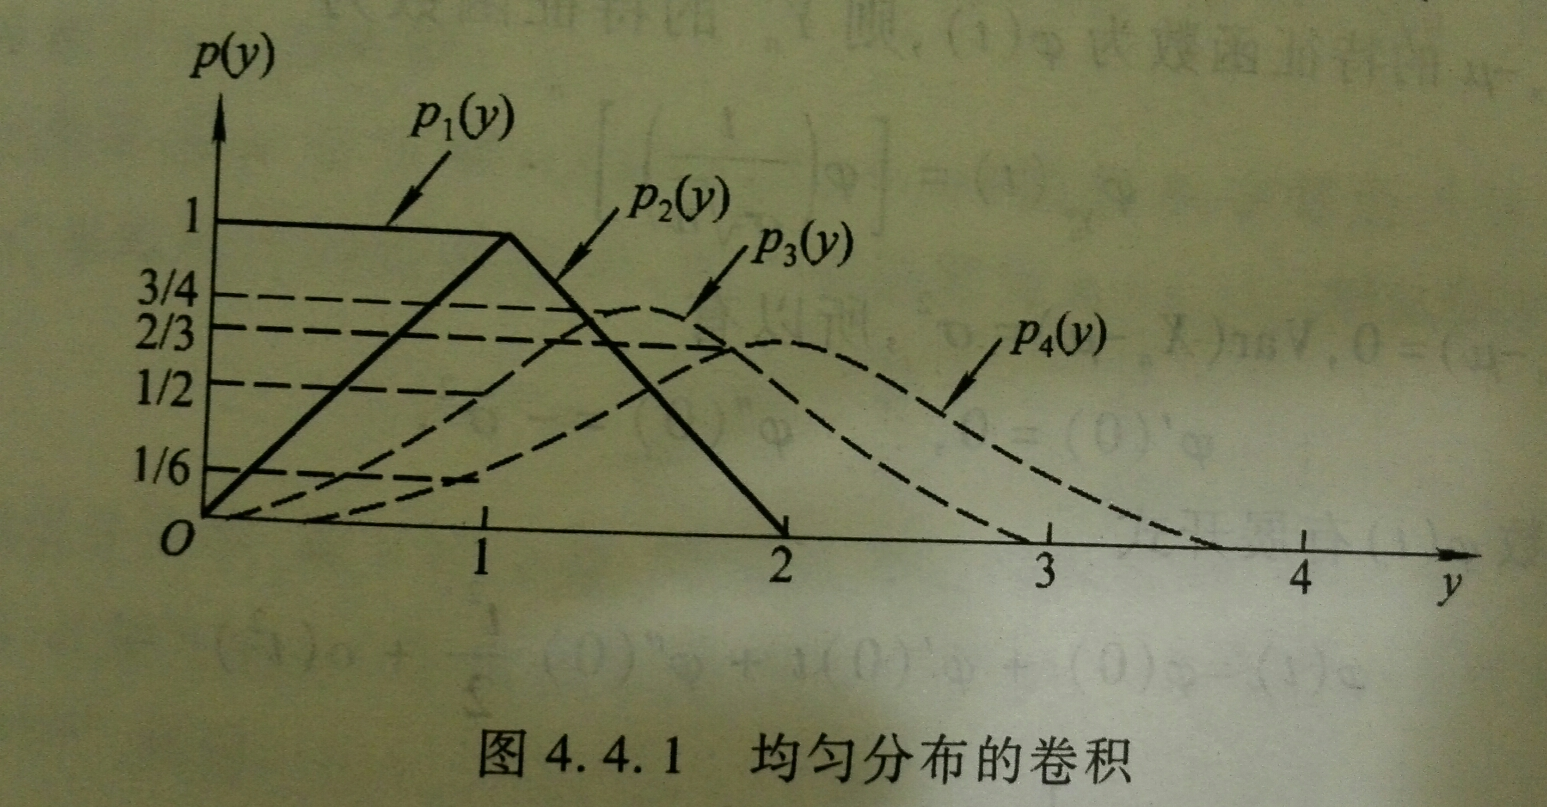
\includegraphics[width=9cm]{uniform.jpg}
	\end{figure}

\end{frame}

\begin{frame}
	\frametitle{问题:寻求 $Y_n$ 的极限分布}
	\begin{itemize}[<+-|alert@+>]
		\item 从上面均匀分布的例子可知:
		\begin{eqnarray*}
			E(Y_n)=\pause \sum_{i=1}^nE(X_i)=\dfrac{n}{2}\rightarrow\infty\\
			D(Y_n)=\pause \sum_{i=1}^n D(X_i)=\dfrac{n}{12}\rightarrow\infty
		\end{eqnarray*}
		\item 考虑 $Y_n$ 的极限分布时,需对 $Y_n$ 进行标准化:
		\begin{eqnarray*}
			Y_n^*:=\dfrac{Y_n-E(Y_n)}{\sqrt{D(Y_n)}}
		\end{eqnarray*}
		\item 在什么情况下
		\begin{eqnarray*}
			\lim_{n\rightarrow\infty}P(Y_n^*\le y)=\dfrac{1}{\sqrt{2\pi}}\int_{-\infty}^ye^{-u^2/2}du
		\end{eqnarray*}

	\end{itemize}
\end{frame}

\begin{frame}
	\frametitle{独立同分布情形下的中心极限定理}
	\begin{thm}[林德伯格 - 莱维 (Lindeberg-L{\'e} vy) 中心极限定理] 设 $\{X_n\}$ 是独立同分布的随机变量序列,且 $E (X_i)=\mu, D (X_i)=\sigma^2>0$ 存在,若记
		\begin{eqnarray*}
			Y_n^*=\dfrac{\sum_{i=1}^nX_i-n\mu}{\sigma\sqrt{n}},
		\end{eqnarray*}
		则对任意的 $y\in R$ 有
		\begin{eqnarray*}
			\lim_{n\rightarrow\infty}P(Y_n^*\le y)=\dfrac{1}{\sqrt{2\pi}}\int_{-\infty}^ye^{-u^2/2}du
		\end{eqnarray*}

	\end{thm}
\end{frame}
\begin{frame}
	\frametitle{Lindeberg-L{\'e}vy 中心极限定理的证明}
	\zheng 要证 $Y_n^*$ 依分布收敛于标准正态分布,只需要说明其特征函数收敛于标准正态分布的特征函数即可. \pause 注意到 $Y_n^*=\sum_{i=1}^n\dfrac{X_i-\mu}{\sigma\sqrt{n}}$. 故若记 $Z_i:=X_i-\mu$ 的特征函数为 $\varphi (t)$, 则
	\begin{eqnarray*}
		\varphi(t)&=&\pause \varphi(0)+\varphi'(0)t+\varphi''(0)\frac{t^2}{2}+o(t^2)\\
		&=&\pause 1+iE(Z_i)+i^2E(Z_i^2)\frac{t^2}{2}+o(t^2)\\
		&=&\pause 1-\frac{\sigma^2t^2}{2}+o(t^2)\\
		\varphi_{Y_n^*}&=&\pause \bigg[\varphi(\frac{t}{\sigma\sqrt{n}})\bigg]^n=\pause \bigg[1-\frac{t^2}{2n}+o(\frac{t^2}{n\sigma^2})\bigg]^n\rightarrow \pause e^{-t^2/2}
	\end{eqnarray*}

\end{frame}
\begin{frame}
	\frametitle{标准正态随机数的产生}
	\begin{itemize}[<+-|alert@+>]
		\item 在随机模拟中经常会需要产生正态随机数,下面我们介绍一种利用中心极限定理通过 $(0,1)$ 上的均匀分布的随机数来产生正态分布 $N (\mu,\sigma^2)$ 随机数的方法;
		\item 中心极限定理理论分析:设 $X_1,\cdots,X_n,\cdots$ 为一列独立同 $(0,1)$ 上的均匀分布的随机变量序列,则 $E (X_i)=1/2, D (X_i)=1/12$, 故
		\begin{eqnarray*}
			\dfrac{\sum_{i=1}^nX_i-n/2}{\sqrt{n/12}}\rightarrow~ \sim N(0,1)
		\end{eqnarray*}
		特别的,若 $n=12$, 则 $X_1+X_2+\cdots+X_{12}-6$ 近似服从标准正态分布.
		\item 产生正态随机数的方法:
		\begin{itemize}
			\item 从计算机中产生 12 个 $(0,1)$ 上均匀分布随机数,记为 $x_1,\cdots, x_{12}$;
			\item 计算 $y=x_1+\cdots+x_{12}-6$, 由上面分析知可将 $y$ 看成 $N (0,1)$ 的一个随机数;
			\item 计算 $z=\mu+\sigma y$, 可将 $z$ 看成 $N (\mu,\sigma^2)$ 分布的随机数;
			\item 重复上面步骤 $n$ 次,即可得到 $n$ 个 $N (\mu,\sigma^2)$ 分布随机数.
		\end{itemize}

	\end{itemize}
\end{frame}
% \begin{frame}
	%   \frametitle{数值计算中的误差分析 I}
	%   \begin{itemize}[<+-|alert@+>]
		%   \item 在数值计算中,任何实数 $x$ 只能通过一定位数的小数 $x'$ 来近似,不妨设我们用四舍五入法得到的 $k$ 位小数来近似;
		%   \item 若 $x'=a_0.a_1a_2\cdots a_k$, 则 $\epsilon:=x-x'\in (-0.5*10^{-k},0.5*10^{-k})$;
		%   \item 考虑一般情形,对于任何实数 $x$, 假设我们通过某种方法选取某个 $k$ 位小数 $x'$ 近似 $x$ 并且假设其误差 $\epsilon$ 服从 $(-0.5*10^{-k},0.5*10^{-k})$ 上的均匀分布 $U (-0.5*10^{-k},0.5*10^{-k})$;
		%   \item 考虑 $n$ 个实数 $x_1,\cdots, x_n$ 的和 $S$ 的近似值 $S'$: 假设 $S$ 中的每一个 $x_i$ 均采用上述一般情形下的近似方法获得其近似值 $x'$, 如果记个别误差为 $\epsilon_i:=x_i-x_i'$, 则总误差为
		%     \begin{eqnarray*}
			%       S-S'=\sum_{i=1}^n(x_i-x_i')=\sum_{i=1}^n\epsilon_i
			%     \end{eqnarray*}
		%   \item 根所假设,我们可以认为 $\epsilon_i\sim U (-0.5*10^{-k},0.5*10^{-k})$, 且相互独立.
		%   \end{itemize}
	% \end{frame}
% \begin{frame}
	%   \begin{columns}
		%     \column{5cm}
		%     \begin{figure}
			%       \centering
			%       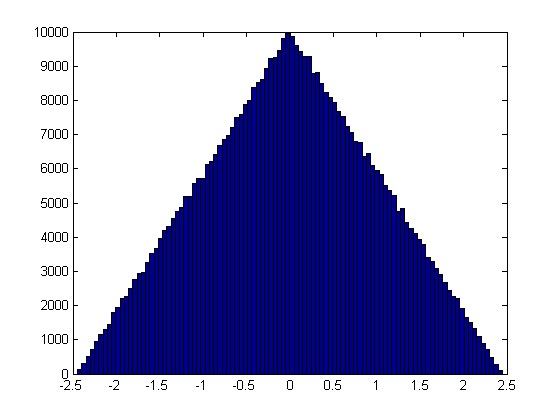
\includegraphics[width=5cm]{2sumuniform.png}
			%     \end{figure}
		%     \column{5cm}
		%     \begin{figure}
			%       \centering
			%       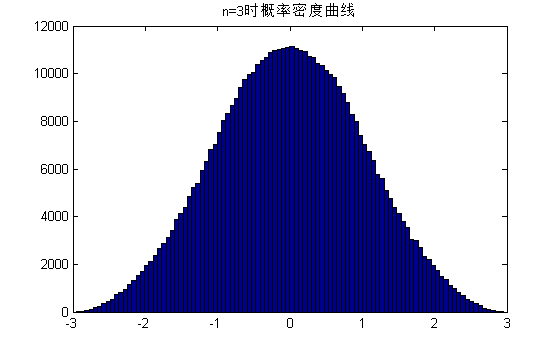
\includegraphics[width=5cm]{3sumuniform.png}
			%     \end{figure}

		%   \end{columns}
	%   \begin{columns}
		%     \column{5cm}
		%     \begin{figure}
			%       \centering
			%       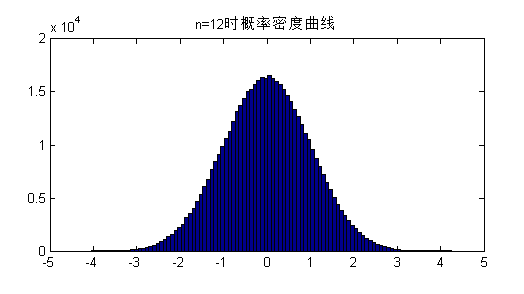
\includegraphics[width=5cm]{12sumuniform1.png}
			%     \end{figure}
		%     \column{5cm}
		%     \begin{figure}
			%       \centering
			%       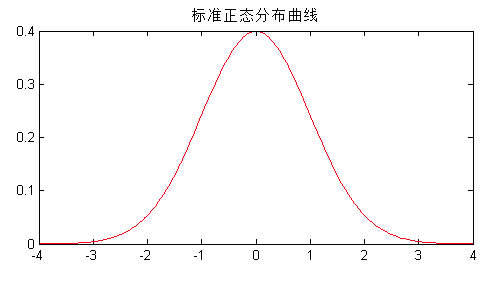
\includegraphics[width=5cm]{n01.png}
			%     \end{figure}

		%   \end{columns}
	% \end{frame}
% \begin{frame}
	%   \frametitle{数值计算中的误差分析 II}
	%   \begin{itemize}[<+-|alert@+>]
		%   \item 一种粗略的估计总误差的方法为:由于 $|\epsilon_i|\le 0.5*10^{-k}$, 故
		%     \begin{eqnarray*}
			%       |\sum_{i=1}^n\epsilon_i|\le n*0.5*10^{-k}
			%     \end{eqnarray*}
		%   \item 利用中心极限定理: $\epsilon_i$ 独立同分布且 $E (\epsilon_i)=0,D (\epsilon_i)=\dfrac{10^{-2k}}{12}$, 故
		%{\small\begin{eqnarray*}
				%              P(\sum_{i=1}^n\epsilon_i|\le z)&=&\pause P(\bigg|\dfrac{\sum_{i=1}^n\epsilon_i-0}{\sqrt{n10^{-2k}/12}}\bigg|\le \dfrac{z}{\sqrt{n10^{-2k}/12}})\\
				%                                             &\approx&\pause \Phi(\dfrac{z}{\sqrt{n10^{-2k}/12}})-\Phi(-\dfrac{z}{\sqrt{n10^{-2k}/12}})\\
				%                                             &=&\pause 2\Phi(\dfrac{z}{\sqrt{n10^{-2k}/12}})-1
				%            \end{eqnarray*}}
		%        \item 若令上面的概率为 $0.99$, 则 $\Phi (\dfrac{z}{\sqrt{n10^{-2k}/12}})=0.995$, 反查正态分布函数表可得 \vspace{-0.7cm}
		%          \begin{eqnarray*}
			%            \hspace{1.2cm} \dfrac{z}{\sqrt{n10^{-2k}/12}}=2.576\Rightarrow z=2.576\sqrt{n10^{-2k}/12}
			%          \end{eqnarray*}

		%        \end{itemize}


	%      \end{frame}

\begin{frame}
	\frametitle{二项分布的正态近似}
	\begin{thm}[棣莫弗 - 拉普拉斯中心极限定理] 设 $n$ 重伯努利试验中,事件 $A$ 在每次试验中出现的概率为 $p\in (0,1)$, 记 $S_n$ 为 $n$ 重伯努利试验中事件 $A$ 出现的次数,则对任意的 $y\in R$ 均有
		\begin{eqnarray*}
			\lim_{n\rightarrow\infty}P(\dfrac{S_n-np}{\sqrt{np(1-p)}}\le y)=\dfrac{1}{\sqrt{2\pi}}\int_{-\infty}^ye^{-u^2/2}du
		\end{eqnarray*}

	\end{thm}
	\pause 在上述定理中,若记 $\Phi (y)=\beta, Y_n^*:=\dfrac{S_n-np}{\sqrt{np (1-p)}}$, 则
	\begin{eqnarray*}
		P(Y_n^*\le y)\approx \Phi(y)=\beta
	\end{eqnarray*}


\end{frame}

% \begin{frame}
	%   \frametitle{二项分布正态近似的几点注意}
	%   \begin{itemize}[<+-|alert@+>]
		%   \item 与二项分布的泊松近似相比:一般来说,$p$ 较小时,用泊松分布近似较好;而在 $np>5$ 和 $n (1-p)>5$ 时,正态分布近似较好;
		%   \item 因二项分布是离散分布,正态分布是连续分布,故用正态分布近似时,作些修正可以提高精度:若 $k_1<k_2$, 一般先作如下修正再用正态近似 $P (k_1\le S_n\le k_2)=P (k_1-0.5<S_n<k_2-0.5)$;
		%   \item 对于二项分布的计算,用修正的正态近似还可得
		%     \begin{eqnarray*}
			%       P(S_n=k)&=&\pause P(k-0.5<S_n<k+0.5)\\
			%               &=&\pause P(\dfrac{k-0.5-np}{\sqrt{np(1-p)}}<\dfrac{S_n-np}{\sqrt{np(1-p)}}<\dfrac{k+0.5-np}{\sqrt{np(1-p)}})\\
			%               &\approx&\pause\int_{\frac{k-0.5-np}{\sqrt{np(1-p)}}}^{\frac{k+0.5-np}{\sqrt{np(1-p)}}} \dfrac{1}{\sqrt{2\pi}}e^{-x^2/2}dx\\
			%               &\approx&\pause \dfrac{1}{\sqrt{2\pi}}e^{-(\frac{k-np}{\sqrt{np(1-p)}})^2/2}\cdot \dfrac{1}{\sqrt{np(1-p)}}
			%     \end{eqnarray*}

		%   \end{itemize}

	% \end{frame}
\begin{frame}
	\frametitle{独立不同分布下的中心极限定理}
	\begin{itemize}[<+-|alert@+>]
		\item 设 $\{X_n\}$ 是一个相互独立的随机变量序列,其期望与方差有限分别为
		\begin{eqnarray*}
			E(X_i)=\mu_i, \quad D(X_i)=\sigma_i^2, \quad i=1,2,\cdots,
		\end{eqnarray*}
		\item 考虑随机变量的和 $\textcolor{red}{Y_n=X_1+\cdots+X_n}$, 则
		\begin{eqnarray*}
			E(Y_n)=\mu_1+\cdots+\mu_n,\quad \textcolor{red}{\sigma(Y_n):=\sqrt{D(Y_n)}=\sqrt{\sigma_1^2+\cdots+\sigma_n^2}}
		\end{eqnarray*}
		\item 考虑 $Y_n$ 的标准化:$ Y_n^*:=\dfrac{Y_n-E (Y_n)}{\sigma (Y_n)}=\sum_{i=1}^n\dfrac{X_i-\mu_i}{\sigma (Y_n)}$
		\item 要求 $Y_n^*$ 中的各项 $\dfrac{X_i-\mu_i}{\sigma (Y_n)}$ 均匀的小,即对任意的 $\tau>0$, 要求事件
		\begin{eqnarray*}
			A_{ni}=\left\{\dfrac{X_i-\mu_i}{\sigma(Y_n)}>\tau\right\}=\left\{|X_i-\mu_i|>\tau\sigma(Y_n)\right\}
		\end{eqnarray*}
		发生的可能性小或直接要求其概率趋于 0.
		\item 为达目的,我们要求 $\lim_{n\rightarrow\infty} P (\max_{1\le i\le n}|X_i-\mu_i|>\tau\sigma (Y_n))=0$
	\end{itemize}
\end{frame}
\begin{frame}
	\frametitle{$\lim_{n\rightarrow\infty}P(\max_{1\le i\le n}|X_i-\mu_i|>\tau\sigma(Y_n))=0$}
	注意到
	\begin{eqnarray*}
		&&P(\max_{1\le i\le n}|X_i-\mu_i|>\tau\sigma(Y_n))=\pause P(\cup_{i=1}^n|X_i-\mu_i|>\tau\sigma(Y_n))\\
		&&\le\pause \sum_{i=1}^nP(|X_i-\mu_i|>\tau\sigma(Y_n))=\pause \sum_{i=1}^n\int_{|x-\mu_i|>\tau\sigma(Y_n)}dF_i(x)\\
		&&\le \pause \dfrac{1}{\tau^2\sigma(Y_n)^2}\sum_{i=1}^n\int_{|x-\mu_i|>\tau\sigma(Y_n)}(x-\mu_i)^2dF_i(x)
	\end{eqnarray*}

	\pause 故只要下面的 \textcolor{red}{\bf 林德伯格条件} 满足
	\begin{eqnarray*}%\label{eq:Lindeberg}
		\lim_{n\rightarrow\infty} \dfrac{1}{\tau^2\sigma(Y_n)^2}\sum_{i=1}^n\int_{|x-\mu_i|>\tau\sigma(Y_n)}(x-\mu_i)^2dF_i(x)=0
	\end{eqnarray*}
	就可保证 $Y_n^*$ 中各加项充分的小


\end{frame}

\begin{frame}
	\frametitle{林德伯格中心极限定理}
	\begin{thm}
		设独立随机变量序列 $\{X_n\}$ 满足林德伯格条件
		\begin{eqnarray}\label{eq:Lindeberg}
			\lim_{n\rightarrow\infty} \dfrac{1}{\tau^2\sigma(Y_n)^2}\sum_{i=1}^n\int_{|x-\mu_i|>\tau\sigma(Y_n)}(x-\mu_i)^2dF_i(x)=0
		\end{eqnarray} 则对任意的 $x$, 有
		\begin{eqnarray*}
			\lim_{n\rightarrow\infty}P(\dfrac{1}{\sigma(Y_n)}\sum_{i=1}^n(X_i-\mu_i)\le x)=\dfrac{1}{\sqrt{2\pi}}\int_{-\infty}^xe^{-u^2/2}du
		\end{eqnarray*}
	\end{thm}
	\pause
	\begin{rmk}
		假设 $\{X_n\}$ 独立同分布且方差有限,则容易验证上述的林德伯格条件满足,从而我们先前在独立同分布情形下的中心极限定理是林德伯格中收极限定理的特例.
	\end{rmk}
\end{frame}

\begin{frame}{一个引理}
	\begin{lem}\label{lem:eixtaylor}
		对一切 $x \in R$ 及非负整数 $n$ 有
		\[
		\left|e^{i x}-\sum_{k=0}^{n} \frac{(i x)^{k}}{k!}\right| \leq\left[\frac{|x|^{n+1}}{(n+1)!}\right] \wedge\left[\frac{2|x|^{n}}{n!}\right]
		\]
	\end{lem}

\end{frame}
\begin{frame}{引理证明}
\begin{itemize}
	\item 用分部积分可得
	\begin{align}\label{eq:sepinte}
		\int_{0}^{x}(x-s)^{n} e^{i s} d s=\frac{x^{n+1}}{n+1}+\frac{i}{n+1} \int_{0}^{x}(x-s)^{n+1} e^{i s} d s
	\end{align}

	\item 递归可得知,对一切 $n \geq 0$ 有
	\begin{align}\label{eq:digui}
		e^{i x}=\sum_{k=0}^{n} \frac{(i x)^{k}}{k!}+\frac{i^{n+1}}{n!} \int_{0}^{x}(x-s)^{n} e^{i s} d s
	\end{align}

	\item
	由此推出估计式$
	\big|e^{i x}-\sum_{k=0}^{n} \dfrac{(i x)^{k}}{k!}\big| \leq \dfrac{|x|^{n+1}}{(n+1)!}$
	\item 将\eqref{eq:sepinte}式中 $n$ 换为 $n-1$ ,解出右方积分并代入\eqref{eq:digui}便推出
	\[
	e^{i x}=\sum_{k=0}^{n} \frac{(i x)^{k}}{k!}+\frac{i^{n}}{(n-1)!} \int_{0}^{x}(x-s)^{n-1}\left(e^{i s}-1\right) d s
	\]
\item 故可得另一估计式$
	\left|e^{i x}-\sum_{k=0}^{n} \dfrac{(i x)^{k}}{k!}\right| \leq \dfrac{2|x|^{n}}{n!}$
\item 联合上述两个估计式可得引理结论.%(4.10)与(4.11)便得到(4.7)式,引理证完。


\end{itemize}

\end{frame}
\begin{frame}{引理的几个常用结论}
\begin{rmk} 若引理中的$n=0,1,2$, 则有%的特例以备引用:
	\begin{align*}
		\left|e^{i x}-1\right| & \leq|x| \wedge 2 \\
		\left|e^{i x}-1-i x\right| & \leq \frac{x^{2}}{2} \wedge(2|x|) \\
		\left|e^{i x}-1-i x+\frac{x^{2}}{2}\right| & \leq\left(\frac{1}{6}|x|^{3}\right) \wedge x^{2}
	\end{align*}
\end{rmk}

\end{frame}

\begin{frame}{林德伯格中心极限定理证明}
\begin{itemize}
	\item 只需证 $Y_n^*:=\frac{\sum_{k=1}^n(X_k-E[X_k])}{\sqrt{D(\sum_{k=1}^nX_k)}}$ 的特征函数列收敛到标准正态分布的特征函数,即
	\begin{align}\label{eq:celimit}
		\lim_{n\rightarrow\infty}\phi_{n}(t)=\lim_{n\rightarrow\infty}E[e^{itY_n^*}]= \exp\{-\frac{t^2}{2}\}.
	\end{align}

    \item 对一切 $n \geq 1$ 及 $k=1, \cdots, n$,令 $X_{nk}=\left(X_{k}-\mu_k\right) / \sigma(Y_n)$, 则
	\[E\left(X_{nk}\right)=0,\quad D\left(X_{nk}\right)=\sigma_k^{2} / \sigma(Y_n)^{2}.\]
	\item 以 $F_{n k}(x)$ 及 $\phi_{n k}(t)$ 分别表 $X_{nk}$的分布函数及特征函数.
		\item 已知的林德伯格条件\eqref{eq:Lindeberg}式化为
		\begin{align}\label{eq:Lindebergcondi-2}
			\lim _{n} \sum_{k=1}^{n} \int_{(|x| \geq \tau)} x^{2} d F_{n k}(x)=0, \ \forall \tau>0
		\end{align}

	\item
		而待证的\eqref{eq:celimit}式变为 $n \rightarrow \infty$ 时有
		\[
		\phi_{n}(t)=\prod_{k=1}^{n} \phi_{n k}(t) \longrightarrow \exp\{-\frac{t^2}{2}\},  \forall t \in R
		\]

\end{itemize}

\end{frame}
\begin{frame}{林德伯格中心极限定理证明}
	\begin{itemize}
		\item 注意到
		\begin{align*}
		  \phi_{nk}(t)&\approx 1+\phi_{nk}'(0)t+\frac{1}{2}\phi_{nk}''(0)t^2=1+iE[X_{nk}]t+\frac{1}{2}i^2E[X_{nk}^2]t^2\\
					&=1-\frac{t^2\sigma_k^2}{2\sigma(Y_n)^2}\approx \exp\{-\frac{t^2\sigma_k^2}{2\sigma(Y_n)^2}\}\\
			\exp\{-\frac{t^2}{2}\}&=\exp\{-\frac{t^2}{2}\sum_{k=1}^n\frac{\sigma_k^2}{\sigma(Y_n)^2}\}=\prod_{k=1}^{n} \exp\{-\frac{t^2\sigma_k^2}{2\sigma(Y_n)^2}\}
		\end{align*}
		\item 因此,欲证$\phi_{n}(t)=\prod_{k=1}^{n} \phi_{n k}(t) \longrightarrow e^{-\frac{t^{2}}{2}},  \forall t \in R$, 只需证明
		\begin{align*}
	&\big|\prod_{k=1}^{n} \phi_{n k}(t)-\prod_{k=1}^{n}\big(1-\frac{t^{2} \sigma_{k}^{2}}{2 \sigma(Y_n)^2}\big)\big| \longrightarrow 0\\
	&\big|\prod_{k=1}^{n}\big(1-\frac{t^{2} \sigma_{k}^{2}}{2 \sigma(Y_n)^2}\big)-\prod_{k=1}^{n} \exp\{-\frac{t^2\sigma_k^2}{2\sigma(Y_n)^2}\}\big| \longrightarrow 0
		\end{align*}
	\end{itemize}


	\end{frame}
	\begin{frame}{证明:$\big|\prod_{k=1}^{n} \phi_{n k}(t)-\prod_{k=1}^{n}\big(1-\frac{t^{2} \sigma_{k}^{2}}{2 \sigma(Y_n)^2}\big)\big| \rightarrow 0$}
		\vspace{-0.1cm}
		\begin{itemize}
			\item 由引理\ref{lem:eixtaylor}可知,对一切 $t \in R$ 有
		\[
		\big|e^{i t x}-\big(1+i t x-\frac{1}{2} t^{2} x^{2}\big)\big| \leq|t x|^{2} \wedge|t x|^{3}
		\]
		\item 注意到 $X_{nk}$ 二阶矩有限,两边对 $F_{n k}$ 取积分得
		\[
		\big|\phi_{n k}(t)-\big(1-\frac{t^{2} \sigma_{k}^{2}}{2 \sigma(Y_n)^{2}}\big)\big| \leq E\big\{\big|t X_{nk}\big|^{2} \wedge\big|t X_{nk}\big|^{3}\big\}
		\]
		\item 而对任何 $\tau>0$ ,上式右方不超过
		\begin{align*}
			&\int_{(|x|<\tau)}|t x|^{3} d F_{n k}(x)+\int_{(|x| \geq \tau)}(t x)^{2} d F_{n k}(x)\\
			&\leq \tau|t|^{3} \frac{\sigma_{k}^{2}}{\sigma(Y_n)^{2}}+t^{2} \int_{(|x| \geq \tau)} x^{2} d F_{n k}(x)
		\end{align*}
		\item 由于 $\sum_{k=1}^{n} \sigma_{k}^{2} / \sigma(Y_n)^{2}=D\big(Y_n^*\big)=1$, 求和便推出
		\[
		\sum_{k=1}^{n}\big|\phi_{n k}(t)-\big(1-\frac{t^{2} \sigma_{k}^{2}}{2 \sigma(Y_n)^{2}}\big)\big| \leq \tau|t|^{3}+t^{2} \sum_{k=1}^{n} \int_{(|x| \geq \tau)} x^{2} d F_{n k}(x)
		\]
		\end{itemize}
	\end{frame}

	\begin{frame}{证明:$\big|\prod_{k=1}^{n} \phi_{n k}(t)-\prod_{k=1}^{n}\big(1-\frac{t^{2} \sigma_{k}^{2}}{2 \sigma(Y_n)^2}\big)\big| \rightarrow 0$}
\begin{itemize}
	\item 上式先令 $n \rightarrow \infty$ 再令 $\tau \downarrow 0$, 由\eqref{eq:Lindebergcondi-2}式得
	\[
	\sum_{k=1}^{n}\big|\phi_{n k}(t)-\big(1-\frac{t^{2} \sigma_{k}^{2}}{2 \sigma(Y_n)^2}\big)\big| \rightarrow 0,  t \in R
	\]
	\item 故
	\begin{align*}
		\big|\prod_{k=1}^{n} \phi_{n k}(t)-\prod_{k=1}^{n}\big(1-\frac{t^{2} \sigma_{k}^{2}}{2 \sigma(Y_n)^2}\big)\big|\leq  \sum_{k=1}^{n}\big|\phi_{n k}(t)-\big(1-\frac{t^{2} \sigma_{k}^{2}}{2 \sigma(Y_n)^2}\big)\big| \rightarrow 0
	\end{align*}得证.
\end{itemize}
	\end{frame}

\begin{frame}{证明:$\big|\prod_{k=1}^{n}\big(1-\frac{t^{2} \sigma_{k}^{2}}{2 \sigma(Y_n)^2}\big)-\prod_{k=1}^{n} \exp\{-\frac{t^2\sigma_k^2}{2\sigma(Y_n)^2}\}\big| \rightarrow 0$}
\vspace{-0.1cm}
\begin{itemize}

	\item 注意到当 $|z| \leq 1 / 2$ 时有
	{\small \[
	\left|e^{z}-1-z\right| \leq \frac{1}{2} \sum_{k=2}^{\infty}|z|^{k}=\frac{1}{2}|z|^{2} /(1-|z|) \leq z^{2}
	\]}
    \item 取 $z=\frac{t^{2} \sigma_{k}^{2}}{2 \sigma(Y_n)^2}$, 可得
    {\small \begin{align*}
		&\big|\prod_{k=1}^{n}\big(1-\frac{t^{2} \sigma_{k}^{2}}{2 \sigma(Y_n)^2}\big)-\prod_{k=1}^{n} \exp\{-\frac{t^2\sigma_k^2}{2\sigma(Y_n)^2}\}\big|\\
		&\leq \sum_{k=1}^{n}\big|\exp\{-\frac{t^2\sigma_k^2}{2\sigma(Y_n)^2}\}-\big(1-\frac{t^{2} \sigma_{k}^{2}}{2 \sigma(Y_n)^2}\big)\big|\\
		&\leq \frac{t^4}{4}\sum_{k=1}^{n}\big(\frac{\sigma_{k}^{2}}{\sigma(Y_n)^2}\big)^2\leq \frac{t^{4}}{4}\left(\max _{1 \leq k \leq n} \frac{\sigma_{k}^{2}}{\sigma(Y_n)^2}\right) \sum_{k=1}^{n} \frac{\sigma_{k}^{2}}{\sigma(Y_n)^2}\\
		&\leq \frac{t^{4}}{4}\left(\max _{1 \leq k \leq n} \frac{\sigma_{k}^{2}}{\sigma(Y_n)^2}\right)
	\end{align*}}
	\item 若$\max _{1 \leq k \leq n} \frac{\sigma_{k}^{2}}{\sigma(Y_n)^2}\rightarrow 0$, 则定理得证.
\end{itemize}

\end{frame}


\begin{frame}{证明: $\max _{1 \leq k \leq n} \frac{\sigma_{k}^{2}}{\sigma(Y_n)^2}\rightarrow 0$}
	\vspace{-0.1cm}
\begin{itemize}
	\item 对任何 $\tau>0$ 有
\begin{align*}
	\frac{\sigma_{k}^{2}}{\sigma(Y_n)^2}=D\left(X_{n k}\right)&=\int_{-\infty}^{+\infty}x^2dF_{nk}(x)\\
	&=\int_{|x|<\tau}x^2dF_{nk}(x)+\int_{|x|\geq\tau}x^2dF_{nk}(x)\\
	&\leq \tau^{2}+\int_{(|x| \geq \tau)} x^{2} d F_{n k}(x)
\end{align*}
\item 从而
	\[
	\max _{1 \leq k \leq n} \frac{\sigma_{k}^{2}}{\sigma(Y_n)^2} \leq \tau^{2}+\sum_{k=1}^{n} \int_{(|x| \geq \tau)} x^{2} d F_{n k}(x)
	\]
\item
	再次令 $n \rightarrow \infty$ 及 $\tau \downarrow 0$, 由\eqref{eq:Lindebergcondi-2}式得
	\[
	\lim _{n}\left\{\max _{1 \leq k \leq n} \frac{\sigma_{k}^{2}}{\sigma(Y_n)^2}\right\}=0
	\]
	\item 进而, 若$z=\frac{t^{2} \sigma_{k}^{2}}{2 \sigma(Y_n)^2}$, 当$n$充分大时$|z| \leq 1 / 2$.
\end{itemize}

\end{frame}








\begin{frame}
	\frametitle{推出 Lindeberg 条件的充分条件}
	\begin{thm}
		设 $\{X_n\}$ 为独立随机变量序列,如果存在常数列 $\{L_n\}$ 使得
		\begin{eqnarray*}
			\max_{1\leq k\leq n}|X_k|\leq L_n, \mbox{ 且 } \lim_{n}\dfrac{L_n}{\sigma(Y_n)}=0
		\end{eqnarray*}
		则 Lindeberg 条件成立,从而 $\{X_n\}$ 满足中心极限定理.
	\end{thm}

\zheng
\begin{itemize}
	\item 由假设知,对于 $\tau>0$ ,存在 $N$ ,使当 $n \geq N$ 时有 $2 L_{n}<$ $\tau \sigma(Y_n)$.
	\item 因此当 $n \geq N$ 时对一切 $k=1, \cdots, n$ 有 $\Omega=\left\{\left|X_{k}-\mu_{k}\right|<\tau \sigma(Y_n)\right\}$.
	\item 故 $n \geq N$ 时有
	\begin{align*}
		&\frac{1}{\sigma(Y_n)^{2}} \sum_{k=1}^{n} \int_{\left(\left|x-\mu_{k}\right|<\tau \sigma(Y_n)\right)}\left(x-\mu_{k}\right)^{2} d F_{k}(x)\\
		&=\frac{1}{\sigma(Y_n)^{2}} \sum_{k=1}^{n} \int_{-\infty}^\infty\left(x-\mu_{k}\right)^{2} d F_{k}(x)=1 .
	\end{align*}
\item 这表明林德伯格条件\eqref{eq:Lindeberg} 式成立,故 $\left\{X_{n}\right\}$ 满足中心极限定理.
\end{itemize}




\end{frame}

\begin{frame}
	\frametitle{李雅普诺夫中心极限定理}
	\begin{thm} 设 $\{X_n\}$ 为独立随机变量序列,若存在 $\delta>0$ 满足
		\begin{eqnarray*}
			\lim_{n\rightarrow\infty}\dfrac{1}{\sigma(Y_n)^{2+\delta}}\sum_{k=1}^nE(|X_k-\mu_k|^{2+\delta})=0,
		\end{eqnarray*}
		则 $\lim_{n\rightarrow\infty}P(\dfrac{1}{\sigma(Y_n)}\sum_{k=1}^n(X_k-\mu_k)\le x)=\dfrac{1}{\sqrt{2\pi}}\int_{-\infty}^xe^{-u^2/2}du$.
		% \begin{eqnarray*}
		% 	\lim_{n\rightarrow\infty}P(\dfrac{1}{\sigma(Y_n)}\sum_{i=1}^n(X_i-\mu_i)\le x)=\dfrac{1}{\sqrt{2\pi}}\int_{-\infty}^xe^{-u^2/2}du
		% \end{eqnarray*}

	\end{thm}

	\zheng 只要验证林德伯格条件成立. 实际上对任何 $\tau>0$ 有
	\begin{align*}
		& \lim _{n} \frac{1}{\sigma(Y_n)^{2}} \sum_{k=1}^{n} \int_{\left(\left|x-\mu_k\right| \geq \tau \sigma(Y_n)\right)}\left(x-\mu_{k}\right)^{2} d F_{k}(x) \\
		\leq & \lim _{n} \frac{1}{\sigma(Y_n)^{2}\left(\tau \sigma(Y_n)\right)^{\delta}} \sum_{k=1}^{n} \int_{\left(\left|x-\mu_k\right| \geq \tau \sigma(Y_n)\right)}\left|x-\mu_k\right|^{2+\delta} d F_{k}(x) \\
		\leq & \lim _{n} \frac{1}{\tau^{\delta}} \frac{1}{\sigma(Y_n)^{2+\delta}} \sum_{k=1}^{n} \int_{\Re}\left|x-\mu_{k}\right|^{2+\delta} d F_{k}(x)=0 .
	\end{align*}
	定理证毕.
\end{frame}









 %\input{L11-13-2023.tex}
 %\input{L14-2023.tex}
 %\input{L15-19-2023.tex}%
 %\input{L20-22-2023.tex}%

 %\input{Chapter-01.tex}

 %\input{Chapter-02.tex}
 %\input{Chapter-03.tex}
 %\input{Chapter-04.tex}

 %\input{L10-13.tex}
 %\input{L14-18.tex}

 %\input{L02.tex}

 \end{document}
